\documentclass[preview]{standalone}
%\usepackage{prelude}

%%%%%%%%%%%%%%%%%%%%%%%%%%%%%%%%%%%% PACKAGES %%%%%%%%%%%%%%%%%%%%%%%%%%%%%%%%%%%%%%%%%%

\usepackage{inputenc,fontenc}
\usepackage[a4paper,margin=3cm]{geometry}
\usepackage[english]{babel}
%\usepackage[german]{babel}
%\usepackage[fixlanguage]{babelbib}


\usepackage{bbold}
\usepackage{amsthm}
\usepackage{amsmath}
\usepackage{amssymb} % doteqdot
\usepackage[dvipsnames]{xcolor}
\usepackage{standalone}
\usepackage{tikz}[mode=buildnew]
\usepackage{cite}
\usepackage{xspace}
\usepackage{relsize}
\usepackage{mathtools} % mathclap
%\usepackage{MnSymbol}
\usepackage{hyperref}
\usepackage{url}
\usepackage{listings} % for code
\usepackage[T1]{fontenc} %<
\hypersetup{
	colorlinks,
	citecolor=black,
	filecolor=black,
	linkcolor=black,
	urlcolor=black
}
\usepackage{pgfplots}
\pgfplotsset{compat=1.18}
%\usepackage{courier} %% Sets font for listing as Courier. But also for url and texttt!
\usepackage{listings, xcolor}
\usepackage{graphicx}
\usepackage{subcaption}

\usetikzlibrary{calc}
%\usepackage{xparse} % \newDocumentCommand for multiple optional arguments
%\usepackage{titlecaps}



%%%%%%%%%%%%%%%%%%%%%%%%%%%%%%%%%%%% THEOREMSTYLES %%%%%%%%%%%%%%%%%%%%%%%%%%%%%%%%%%

\theoremstyle{definition}
\newtheorem{definition}{Definition}[section]
\newtheorem{exmp}{Beispiel}[section]
%\AfterEndEnvironment{definition}{\noindent\ignorespaces}

\theoremstyle{theorem}
\newtheorem{theorem}{Satz}[section]
\newtheorem{proposition}{Proposition}[section]
%\AfterEndEnvironment{theorem}{\noindent\ignorespaces}

\theoremstyle{korollary}
\newtheorem{korollary}{Korollar}[section]
%\AfterEndEnvironment{korollary}{\noindent\ignorespaces}


\tikzset{
	mstate/.style={draw, circle, minimum size=.94cm}, 
	gstate/.style={draw, rectangle, minimum size=.8cm},
	varstate/.style={draw,rectangle, rounded corners, minimum size=1}, 
	trans/.style={draw, ->, thick},
	bendtrans/.style={draw, ->, thick, bend left=10},
	bendtransr/.style={draw, ->, thick, bend right=10},
	init/.style={initial, initial distance=6pt, initial text=},
	every loop/.style={min distance=5pt, looseness=8},
	>=latex
}
\usetikzlibrary{automata,positioning}

%auto shift/.style={auto=right,->,
%	to path={ let \p1=(\tikztostart),\p2=(\tikztotarget),
%		\n1={atan2(\y2-\y1,\x2-\x1)},\n2={\n1+180}
%		in ($(\tikztostart.{\n1})!1mm!270:(\tikztotarget.{\n2})$) -- 
%		($(\tikztotarget.{\n2})!1mm!90:(\tikztostart.{\n1})$) \tikztonodes}},

%%%%%%%%%%%%%%%%%%%%%%%%%%%%%%%%%%% MY MACROS %%%%%%%%%%%%%%%%%%%%%%%%%%%%%%%%%%%%%%%%%
%formatting
\newcommand{\comment}[2]{{\color{#1}#2}}
\newcommand{\redcomment}[1]{{\color{red}#1}}
\newcommand{\purpcomment}[1]{{\color{pink}#1}}
\newcommand{\bluecomment}[1]{{\color{blue}#1}}
\newcommand{\mt}[1]{\ensuremath{{#1}}\xspace}
\newcommand{\mynewcommand}[2]{\newcommand{#1}{\mt{#2}}} %% currently not used becaue of ide highlighting
\newcommand{\arr}{\mt{\to}}

%model checking terms
\newcommand{\mimicrel}{\mt{\mathcal{R}}}
\newcommand{\bisimeq}{\mt{\;\!\sim\;\!}}
\newcommand{\simorder}{\mt{\;\!\preceq\;\!}}
\newcommand{\simequiv}{\mt{\;\!\simeq\;\!}} %command already defined
\newcommand{\relts}{\mt{\;\!\bullet_{_{\tiny{TS}}}\;\!}}
\newcommand{\rel}{\mt{\;\!\bullet\;\!}}

%own names
\newcommand{\nm}[1]{#1\xspace}
\newcommand{\mdpN}{\nm{MDP}}
\newcommand{\mdpsN}{\nm{MDPs}}
\newcommand{\viewN}{\nm{view}}
\newcommand{\viewNC}{\nm{View}}
\newcommand{\viewsN}{\nm{views}}
\newcommand{\viewsNC}{\nm{Views}}
\newcommand{\grpfctsubN}{\nm{detached grouping function}}
\newcommand{\grpfctsubNC}{\nm{detached grouping function}}
\newcommand{\grpfctsubNCC}{\nm{Detached Grouping Function}}
\newcommand{\grpfctN}{\nm{grouping function}}
\newcommand{\grpfctNC}{\nm{Grouping function}}
\newcommand{\grpfctNCC}{\nm{Grouping Function}}
\newcommand{\grpfctsN}{\nm{grouping functions}}
\newcommand{\grpfctsNC}{\nm{Grouping functions}}
\newcommand{\grpfctsNCC}{\nm{Grouping Functions}}
\newcommand{\stmimicN}{\nm{state-mimic}}
\newcommand{\stmimicsN}{\nm{state-mimics}}
\newcommand{\stmimickingN}{\nm{state-mimicking}}
\newcommand{\stmimickedN}{\nm{state-mimicked}}
%\newcommand{\chosenphtypeNCC}{\nm{Transition System}}
%\newcommand{\chgphNC}{\nm{Transition system}}
%\newcommand{\chgphN}{\nm{transition system}}
%\newcommand{\chgphsNCC}{\nm{Transition Systems}}
%\newcommand{\chgphsNC}{\nm{Transition systems}}
%\newcommand{\chgphsN}{\nm{transition systems}}
\newcommand{\chgphNCC}{\nm{MDP}}
\newcommand{\chgphNC}{\nm{MDP}}
\newcommand{\chgphN}{\nm{MDP}}
\newcommand{\achgphN}{\nm{an MDP}}
\newcommand{\chgphsNCC}{\nm{MDPs}}
\newcommand{\chgphsNC}{\nm{MDPs}}
\newcommand{\chgphsN}{\nm{MDPs}}
\newcommand{\parllcompN}{\nm{parallel composition}}
\newcommand{\parllcompNC}{\nm{Parallel composition}}
\newcommand{\parllcompNCC}{\nm{Parallel Composition}}
\newcommand{\parllcompsN}{\nm{parallel compositions}}
\newcommand{\parllcompsNC}{\nm{Parallel compositions}}
\newcommand{\parllcompsNCC}{\nm{Parallel Compositions}}
\newcommand{\sccN}{\nm{SCC}}
\newcommand{\sccsN}{\nm{SCCs}}
\newcommand{\bsccN}{\nm{BSCC}}
\newcommand{\bsccsN}{\nm{BSCCs}}
\newcommand{\jgrapht}{\nm{jGraphtT}}

\newcommand{\outactident}{\nm{OutActionsIdent}}

%names
\newcommand{\iffN}{\nm{if and only if}}
\newcommand{\tsN}{\nm{TS}}

%% outactions identical
\newcommand{\outactidentstrong}{\nm{strong}}
\newcommand{\outactidentweak}{\nm{weak}}

% CORE DEFINITIONS
\newcommand{\grpfct}[1][\viewppty]{\mt{F_{#1}}}
\newcommand{\grpfctsub}[1][\viewppty]{\mt{\tilde{F}_{#1}}}
%\newcommand{\grpfctimg}[1]{\mt{{\grpfct}[{#1}]}}
%\newcommand{\fctimg}[2]{\mt{{#1}[{#2}]}}
\newcommand{\eqrelview}{\mt{R}}
\newcommand{\eqclassv}[1][\state]{\mt{\eqclass{#1}{\eqrelview}}}
\newcommand{\eqclasssetv}[1][\states]{\mt{{#1}/\eqrelview}} %OLD: \bigcup_{\state \in \states} \eqclassv
\newcommand{\viewid}{\mt{\mdp}}
\newcommand{\view}[1][\viewppty]{\mt{\viewid_{#1}}}
\newcommand{\imggrp}{\mt{\arbset}}
\newcommand{\imggrpsub}{\mt{X}}
\newcommand{\viewppty}{\mt{\theta}}
\newcommand{\pll}{\mt{\;\!\pllpure\;\!}}
\newcommand{\pllrev}{\mt{\pllpure^{-1}}}
\newcommand{\pllpure}{\mt{||}}
\newcommand{\compselectset}{\mt{Z}}
\newcommand{\compselectpure}{\mt{\pllpure_\compselectset}}
\newcommand{\compselect}{\mt{\;\pllpure_\compselectset\;}}
\newcommand{\remstates}{\mt{\bigcup_{\state \in \states \setminus \states_1}\{\{\state\}\}}}
\newcommand{\nogroupstates}[1][\states_2]{\mt{\bigcup_{\state \in \states \setminus {#1}}\{\{\state\}\}}}
\newcommand{\remelem}{\mt{\bullet}}
\newcommand{\nogroupset}{\mt{\xi}}
\newcommand{\remset}{\mt{\{\remelem\}}}
\newcommand{\gfctpll}{\mt{\grpfct[\pll]}}
\newcommand{\group}{\mt{\top}}
\newcommand{\imggrpbinview}{\mt{\{\remelem, \notppty\}}}
\newcommand{\viewappset}{\mt{\tilde{\states}}}
\newcommand{\hasppty}{\mt{\top}}
\newcommand{\notppty}{\mt{\bot}}
\newcommand{\disregardelem}{\mt{\Delta}}
\newcommand{\disregardelements}{\mt{{\disregardelem_1, \dots, \disregardelem_n}}}



%\newcommand{\mdp}{def}\mdp
%\newcommand{\mdpdef}



% EXAMPLE VIEWS
\newcommand{\pptyatomicprops}{\mt{\atomicprops}}
\newcommand{\pptyinitstates}{\mt{\initstates}}
\newcommand{\pptyinactsetsize}{\mt{|\inacts(\state)|}}
\newcommand{\pptyhasoutact}{\mt{\exists\outact}}
\newcommand{\pptyminoutact}[2]{\mt{#1\leq#2}}
\newcommand{\pptymaxoutact}[2]{\mt{#2\leq#1}}
\newcommand{\pptyspanoutact}[3]{\mt{#1\leq#2\leq#3}}
\newcommand{\pptyoutactsetsize}{\mt{|\outacts(\state)|}}
\newcommand{\pptyoutactsingle}{\mt{|\outacts(\state)|_1}}
\newcommand{\pptystrongoutactident}{\mt{\outacts(\state)_=}}
\newcommand{\pptyweakoutactident}{\mt{\outacts(\state)_\approx}}
\newcommand{\pptyhasinact}{\mt{\exists\inact}}
\newcommand{\pptymininact}[2]{\mt{#1\leq#2}}
\newcommand{\pptymaxinact}[2]{\mt{#2\leq#1}}
\newcommand{\pptyspaninact}[3]{\mt{#1\leq#2\leq#3}}
\newcommand{\pptyinactsingle}{\mt{|\inacts(\state)|_1}}
\newcommand{\pptystronginactident}{\mt{\inacts(\state)_=}}
\newcommand{\pptyweakinactident}{\mt{\inacts(\state)_\approx}}
\newcommand{\pptyparamvalueseq}{\mt{\var = \varval}}
\newcommand{\pptyparamvaluesneq}{\mt{\var \neq \varval}}
\newcommand{\pptyparamdnf}{\mt{VarDNF}}
\newcommand{\pptyparamcnf}{\mt{VarCNF}}
\newcommand{\pptyparamvalueseqopt}{\mt{\var = \varval}}
\newcommand{\pptyparamvalident}{\mt{Var:\varval}}
\newcommand{\pptydistance}{\mt{\distpath}}
\newcommand{\pptydistancerev}{\mt{\distpathrev}}
\newcommand{\pptydistancebi}{\mt{\distpathbi}}
\newcommand{\pptyhascycle}{\mt{\exists\cycle}}
\newcommand{\pptyexactactcycle}{\mt{\{\cycle_{\action,n}\}}}
\newcommand{\pptycycleset}{\mt{\cup{\{\state\}_\cycle}}}
\newcommand{\pptyexactcycle}{\mt{\{\cycle_n\}}}
\newcommand{\pptyscc}{\mt{scc}}
\newcommand{\pptybscc}{\mt{bscc}}
\newcommand{\pptyprop}{\mt{\redcomment{?}}}
\newcommand{\pptyident}{id}


\newcommand{\gfctatomicprops}{\mt{\grpfct[\pptyatomicprops]}}
\newcommand{\gfctinitstates}{\mt{\grpfct[\pptyinitstates]^\hasppty}}
\newcommand{\gfcthasoutaction}{\mt{\grpfct[\pptyhasoutact]^\hasppty}}
\newcommand{\gfctminoutaction}{\mt{\grpfct[\pptyminoutact{\numoutact}{\outact}]^\hasppty}}
\newcommand{\gfctmaxoutaction}{\mt{\grpfct[\pptymaxoutact{\numoutact}{\outact}]^\hasppty}}
\newcommand{\gfctspanoutaction}{\mt{\grpfct[\pptyspanoutact{\numoutactb}{\outact}{\numoutact}]^\hasppty}}
\newcommand{\gfctoutactsetsize}{\mt{\grpfct[\pptyoutactsetsize]}}
\newcommand{\gfctoutactsingle}{\mt{\grpfct[\pptyoutactsingle]^\notppty}}
\newcommand{\gfctstrongoutactident}{\mt{\grpfct[\pptystrongoutactident]}}
\newcommand{\gfctweakoutactident}{\mt{\grpfct[\pptyweakoutactident]}}
\newcommand{\gfcthasinaction}{\mt{\grpfct[\pptyhasinact]^\hasppty}}
\newcommand{\gfctmininaction}{\mt{\grpfct[\pptymininact{\numinact}{\inact}]^\hasppty}}
\newcommand{\gfctmaxinaction}{\mt{\grpfct[\pptymaxinact{\numinact}{\inact}]^\hasppty}}
\newcommand{\gfctspaninaction}{\mt{\grpfct[\pptyspaninact{\numinactb}{\inact}{\numinact}]^\hasppty}}
\newcommand{\gfctinactsetsize}{\mt{\grpfct[\pptyinactsetsize]}}
\newcommand{\gfctinactsingle}{\mt{\grpfct[\pptyinactsingle]^\notppty}}
\newcommand{\gfctstronginactident}{\mt{\grpfct[\pptystronginactident]}}
\newcommand{\gfctweakinactident}{\mt{\grpfct[\pptyweakinactident]}}
\newcommand{\gfctparamvalueseq}{\mt{\grpfct[\pptyparamvalueseq]^\hasppty}}
\newcommand{\gfctparamvaluesneq}{\mt{\grpfct[\pptyparamvaluesneq]^\hasppty}}
\newcommand{\gfctparamdnf}{\mt{\grpfct[\pptyparamdnf]^\hasppty}}
\newcommand{\gfctparamcnf}{\mt{\grpfct[\pptyparamcnf]^\hasppty}}
\newcommand{\gfctparamvalueseqopt}{\mt{\pptyparamvalueseqopt}}
\newcommand{\gfctparamvalident}{\mt{\grpfct[\pptyparamvalident]}}
\newcommand{\gfctdistance}{\mt{\grpfct[\pptydistance]}}
\newcommand{\gfctdistancerev}{\mt{\grpfct[\pptydistancerev]}}
\newcommand{\gfctdistancebi}{\mt{\grpfct[\pptydistancebi]}}
\newcommand{\gfcthascycle}{\mt{\grpfct[\pptyhascycle]}}
\newcommand{\gfctexactcycle}{\mt{\grpfct[\pptyexactcycle]}}
\newcommand{\gfctcycleset}{\mt{\grpfct[\pptycycleset]}}
\newcommand{\gfctexactactcycle}{\mt{\grpfct[\pptyexactactcycle]}}
\newcommand{\gfctscc}{\mt{\grpfct[\pptyscc]}}
\newcommand{\gfctbscc}{\mt{\grpfct[\pptybscc]}}
\newcommand{\gfctprop}{\mt{\grpfct[\pptyprop]}}
\newcommand{\gfctident}{\mt{\grpfct[\pptyident]}}

\newcommand{\gfctsubatomicprops}{\mt{\grpfctsub[\pptyatomicprops]}}
\newcommand{\gfctsubinitstates}{\mt{\grpfctsub[\pptyinitstates]^\hasppty}}
\newcommand{\gfctsubhasoutaction}{\mt{\grpfctsub[\pptyhasoutact]^\hasppty}}
\newcommand{\gfctsubminoutaction}{\mt{\grpfctsub[\pptyminoutact{\numoutact}{\outact}]^\hasppty}}
\newcommand{\gfctsubmaxoutaction}{\mt{\grpfctsub[\pptymaxoutact{\numoutact}{\outact}]^\hasppty}}
\newcommand{\gfctsubspanoutaction}{\mt{\grpfctsub[\pptyspanoutact{\numoutactb}{\outact}{\numoutact}]^\hasppty}}
\newcommand{\gfctsuboutactsetsize}{\mt{\grpfctsub[\pptyoutactsetsize]}}
\newcommand{\gfctsuboutactsingle}{\mt{\grpfctsub[\pptyoutactsingle]^\notppty}}
\newcommand{\gfctsubstrongoutactident}{\mt{\grpfctsub[\pptystrongoutactident]^\hasppty}}
\newcommand{\gfctsubweakoutactident}{\mt{\grpfctsub[\pptyweakoutactident]^\hasppty}}
\newcommand{\gfctsubhasinaction}{\mt{\grpfctsub[\pptyhasinact]}}
\newcommand{\gfctsubmininaction}{\mt{\grpfctsub[\pptymininact{\numinact}{\inact}]}}
\newcommand{\gfctsubmaxinaction}{\mt{\grpfctsub[\pptymaxinact{\numinact}{\inact}]}}
\newcommand{\gfctsubspaninaction}{\mt{\grpfctsub[\pptyspaninact{\numinactb}{\inact}{\numinact}]}}
\newcommand{\gfctsubinactsetsize}{\mt{\grpfctsub[\pptyinactsetsize]^\hasppty}}
\newcommand{\gfctsubinactsingle}{\mt{\grpfctsub[\pptyinactsingle]^\notppty}}
\newcommand{\gfctsubstronginactident}{\mt{\grpfctsub[\pptystronginactident]}}
\newcommand{\gfctsubweakinactident}{\mt{\grpfctsub[\pptyweakinactident]}}
\newcommand{\gfctsubparamvalueseq}{\mt{\grpfctsub[\pptyparamvalueseq]^\hasppty}}
\newcommand{\gfctsubparamvaluesneq}{\mt{\grpfctsub[\pptyparamvaluesneq]^\hasppty}}
\newcommand{\gfctsubparamdnf}{\mt{\grpfctsub[\pptyparamdnf]^\hasppty}}
\newcommand{\gfctsubparamcnf}{\mt{\grpfctsub[\pptyparamcnf]^\hasppty}}
\newcommand{\gfctsubparamvalueseqopt}{\mt{\pptyparamvalueseqopt}}
\newcommand{\gfctsubparamvalident}{\mt{\grpfctsub[\pptyparamvalident]}}
\newcommand{\gfctsubdistance}{\mt{\grpfctsub[\pptydistance]}}
\newcommand{\gfctsubdistancerev}{\mt{\grpfctsub[\pptydistancerev]}}
\newcommand{\gfctsubdistancebi}{\mt{\grpfctsub[\pptydistancebi]}}
\newcommand{\gfctsubhascycle}{\mt{\grpfctsub[\pptyhascycle]^\hasppty}}
\newcommand{\gfctsubexactcycle}{\mt{\grpfctsub[\pptyexactcycle]}}
\newcommand{\gfctsubcycleset}{\mt{\grpfctsub[\pptycycleset]}}
\newcommand{\gfctsubexactactcycle}{\mt{\grpfctsub[\pptyexactactcycle]}}
\newcommand{\gfctsubscc}{\mt{\grpfctsub[\pptyscc]}}
\newcommand{\gfctsubbscc}{\mt{\grpfctsub[\pptybscc]}}
\newcommand{\gfctsubprop}{\mt{\grpfctsub[\pptyprop]}}
\newcommand{\gfctsubident}{\mt{\grpfctsub[\pptyident]}}


\newcommand{\viewatomicprops}{\mt{\view[\pptyatomicprops]}}
\newcommand{\viewinitstates}{\mt{\view[\pptyinitstates]^\hasppty}}
\newcommand{\viewhasoutaction}{\mt{\view[\pptyhasoutact]^\hasppty}}
\newcommand{\viewminoutaction}{\mt{\view[\pptyminoutact{\numoutact}{\outact}]^\hasppty}}
\newcommand{\viewmaxoutaction}{\mt{\view[\pptymaxoutact{\numoutact}{\outact}]^\hasppty}}
\newcommand{\viewspanoutaction}{\mt{\view[\pptyspanoutact{\numoutactb}{\outact}{\numoutact}]^\hasppty}}
\newcommand{\viewoutactsetsize}{\mt{\view[\pptyoutactsetsize]}}
\newcommand{\viewoutactsingle}{\mt{\view[\pptyoutactsingle]^\notppty}}
\newcommand{\viewstrongoutactident}{\mt{\view[\pptystrongoutactident]}}
\newcommand{\viewweakoutactident}{\mt{\view[\pptyweakoutactident]}}
\newcommand{\viewhasinaction}{\mt{\view[\pptyhasinact]^\hasppty}}
\newcommand{\viewmininaction}{\mt{\view[\pptymininact{\numinact}{\inact}]^\hasppty}}
\newcommand{\viewmaxinaction}{\mt{\view[\pptymaxinact{\numinact}{\inact}]^\hasppty}}
\newcommand{\viewspaninaction}{\mt{\view[\pptyspaninact{\numinactb}{\inact}{\numinact}]^\hasppty}}
\newcommand{\viewinactsetsize}{\mt{\view[\pptyinactsetsize]}}
\newcommand{\viewinactsingle}{\mt{\view[\pptyinactsingle]^\notppty}}
\newcommand{\viewstronginactident}{\mt{\view[\pptystronginactident]}}
\newcommand{\viewweakinactident}{\mt{\view[\pptyweakinactident]}}
\newcommand{\viewparamvalueseq}{\mt{\view[\pptyparamvalueseq]}}
\newcommand{\viewparamvaluesneq}{\mt{\view[\pptyparamvaluesneq]}}
\newcommand{\viewparamdnf}{\mt{\view[\pptyparamdnf]^\hasppty}}
\newcommand{\viewparamcnf}{\mt{\view[\pptyparamcnf]^\hasppty}}
\newcommand{\viewparamvalueseqopt}{\mt{\pptyparamvalueseqopt}}
\newcommand{\viewparamvalident}{\mt{\view[\pptyparamvalident]}}
\newcommand{\viewdistance}{\mt{\view[\pptydistance]}}
\newcommand{\viewdistancerev}{\mt{\view[\pptydistancerev]}}
\newcommand{\viewdistancebi}{\mt{\view[\pptydistancebi]}}
\newcommand{\viewhascycle}{\mt{\view[\pptyhascycle]}}
\newcommand{\viewexactcycle}{\mt{\view[\pptyexactcycle]}}
\newcommand{\viewcycleset}{\mt{\view[\pptycycleset]}}
\newcommand{\viewexactactcycle}{\mt{\view[\pptyexactactcycle]}}
\newcommand{\viewscc}{\mt{\view[\pptyscc]}}
\newcommand{\viewbscc}{\mt{\view[\pptybscc]}}
\newcommand{\viewprop}{\mt{\view[\pptyprop]}}
\newcommand{\viewident}{\mt{\view[\pptyident]}}

%\newcommand{\viewatomicprops}{\mt{\view[\atomicprops]}}
%\newcommand{\viewinitstates}{\mt{\view[\initstates]}}
%\newcommand{\viewhasoutaction}{\mt{\view[\pptyhasoutact]}}
%\newcommand{\viewminoutaction}{\mt{\view[\pptyminoutact{\numoutact}{\outact}]}}
%\newcommand{\viewmaxoutaction}{\mt{\view[\pptymaxoutact{\numoutact}{\outact}]}}
%\newcommand{\viewspanoutaction}{\mt{\view[\pptyspanoutact{\numoutactb}{\outact}{\numoutact}]}}
%\newcommand{\viewoutactsetsize}{\mt{\view[\pptyoutactsetsize]}}
%\newcommand{\viewoutactsingle}{\mt{\view[\pptyoutactsingle]}}
%\newcommand{\viewstrongoutactident}{\mt{\view[\outacts(\state)_=]}}
%\newcommand{\viewweakoutactident}{\mt{\view[\outacts(\state)_\approx]}}
%\newcommand{\viewhasinaction}{\mt{\view[\pptyhasinact]}}
%\newcommand{\viewmininaction}{\mt{\view[\pptymininact{\numinact}{\inact}]}}
%\newcommand{\viewmaxinaction}{\mt{\view[\pptymaxinact{\numinact}{\inact}]}}
%\newcommand{\viewspaninaction}{\mt{\view[\pptyspaninact{\numinactb}{\inact}{\numinact}]}}
%\newcommand{\viewinactsetsize}{\mt{\view[\pptyinactsetsize]}}
%\newcommand{\viewinactsingle}{\mt{\view[\pptyinactsingle]}}
%\newcommand{\viewstronginactident}{\mt{\view[\inacts(\state)_=]}}
%\newcommand{\viewweakinactident}{\mt{\view[\inacts(\state)_\approx]}}
%\newcommand{\viewparamvalueseq}{\mt{\view[\var = \varval]}}
%\newcommand{\viewparamvaluesneq}{\mt{\view[\var \neq \varval]}}
%\newcommand{\viewparamdnf}{\mt{\view[VarDNF]}}
%\newcommand{\viewparamcnf}{\mt{\view[VarCNF]}}
%\newcommand{\viewparamvalident}{\mt{\view[\pptyparamvalident]}}
%\newcommand{\viewdistance}{\mt{\view[\pptydistance]}}
%\newcommand{\viewhascycle}{\mt{\view[\exists\cycle]}}
%\newcommand{\viewexactcycle}{\mt{\view[\pptyexactcycle]}}
%\newcommand{\viewcycleset}{\mt{\view[\pptycycleset]}}
%\newcommand{\viewexactactcycle}{\mt{\view[\pptyexactactcycle]}}
%\newcommand{\viewscc}{\mt{\view[scc]}}
%\newcommand{\viewbscc}{\mt{\view[bscc]}}

%actions
\newcommand{\numoutact}{\mt{n}}
\newcommand{\numoutactb}{\mt{m}}
\newcommand{\numinact}{\mt{n}}
\newcommand{\numinactb}{\mt{m}}

\newcommand{\predmaxoutact}[1][\numoutact]{\mt{Q_{\outact\leq#1}(\state,\state_1, \dots, \state_{#1+1})}}
\newcommand{\predminoutact}[1][\numoutact]{\mt{Q_{#1\leq\outact}(\state,\state_1, \dots, \state_{#1})}}
\newcommand{\formoutact}[1][\state]{\mt{C_{#1,\outact}}}
\newcommand{\predmaxinact}[1][\numinact]{\mt{Q_{\inact\leq#1}(\state,\state_1, \dots, \state_{#1+1})}}
\newcommand{\predmininact}[1][\numinact]{\mt{Q_{#1\leq\inact}(\state,\state_1, \dots, \state_{#1})}}

\newcommand{\outact}[1][\action]{\mt{\overrightarrow{#1}}}
\newcommand{\outacts}{\mt{\overrightarrow{\actions}}}
\newcommand{\inact}{\mt{\overleftarrow{\action}}}
\newcommand{\inacts}[1][\action]{\mt{\overleftarrow{#1}}}

%%Parameters
\newcommand{\vars}[1][\mdp]{\mt{V\!ar_{#1}}}
\newcommand{\var}{\mt{x}}
\newcommand{\varstate}[1][]{\mt{\var_{\state#1}}}
\newcommand{\varval}{\mt{a}}
\newcommand{\vareval}[1][\mdp]{\mt{V\!arEval_{#1}}}
\newcommand{\varevalimg}[1][\mdp]{\mt{\vareval[#1][\states,\vars]}}
\newcommand{\varevalimgset}{\mt{\arbset}}
\newcommand{\someparam}{\mt{\tilde{x}}}
\newcommand{\eqorneq}{\mt{\;\doteqdot\;}}
\newcommand{\varstyle}[2]{\mt{\langle#1,#2\rangle}}




%\makeatletter
%\newcommand{\overleftrightsmallarrow}{\mathpalette{\overarrowsmall@\leftrightarrowfill@}}
%\newcommand{\overrightsmallarrow}{\mathpalette{\overarrowsmall@\rightarrowfill@}}
%\newcommand{\overleftsmallarrow}{\mathpalette{\overarrowsmall@\leftarrowfill@}}
%\newcommand{\overarrowsmall@}[3]{%
%	\vbox{%
%		\ialign{%
%			##\crcr
%			#1{\smaller@style{#2}}\crcr
%			\noalign{\nointerlineskip}%
%			$\m@th\hfil#2#3\hfil$\crcr
%		}%
%	}%
%}
%\def\smaller@style#1{%
%	\ifx#1\displaystyle\scriptstyle\else
%	\ifx#1\textstyle\scriptstyle\else
%	\scriptscriptstyle
%	\fi
%	\fi
%}
%\makeatother
%\newcommand{\te}[1]{\overleftrightsmallarrow{#1}}

% Distance
\newcommand{\fctdist}{\mt{distance}}
\newcommand{\fctdistdefault}{\mt{\fctdist(\chgph, \smstates, \grandist)}}
\newcommand{\distval}{\mt{d}}
\newcommand{\grandist}{\mt{n}}
\let\path\oldpath
\newcommand{\path}{\mt{P}}
\newcommand{\pathbi}{\mt{\bar{\path}}}
\newcommand{\pathsecfull}{\mt{(\state_0, \action_0, \state_1, \action_1, \dots, \action_{n}, \state_{n+1})}}
\newcommand{\lenpath}{\mt{len}}
\newcommand{\pfirst}{\mt{first}}
\newcommand{\plast}{\mt{last}}
\newcommand{\pathset}{\mt{\path_\chgph}}
\newcommand{\pathbiset}{\mt{\pathbi_\chgph}}
\newcommand{\distpath}{\mt{\overrightarrow{dist}}}
\newcommand{\distpathrev}{\mt{\overleftarrow{dist}}}
\newcommand{\distpathbi}{\mt{\overline{dist}}}
%Cycles
\newcommand{\cyclesecfull}{\mt{(\state_0, \action_0, \state_1, \action_1, \dots, \action_{n-1}, \state_0)}}
\newcommand{\fctfindcycles}{\mt{findCycles}}
\newcommand{\cycle}{\mt{C}}
\newcommand{\cycleset}{\mt{\cycle_{\mdp, n}}}
\newcommand{\lencycle}{\mt{len}}
% strongly connected components
\newcommand{\scc}{\mt{T}}
\newcommand{\setscc}{\mt{SCC_{\chgph,n}}}
\newcommand{\setbscc}{\mt{BSCC_{\chgph,n}}}

% properties
\newcommand{\propfct}{\mt{f}}

% all Systems
\newcommand{\chgph}{\mt{\mdp}}
\newcommand{\chgphtuple}{\mt{\mdptuple}}
\newcommand{\chgphtupledist}{\mt{\mdptupledist}}

\newcommand{\states}{\mt{S}}
\newcommand{\actions}{\mt{Act}}
\newcommand{\atomicprops}{\mt{AP}}
\newcommand{\labelingfct}{\mt{L}}
\newcommand{\init}{\mt{\initdistrib}} % use MDP % refers to the underlying set
\newcommand{\trans}{\mt{\probtfunc}} % use MDP % refers to the underlying set
\newcommand{\smstates}{\mt{\tilde{\states}}}


\newcommand{\state}{\mt{s}}
\newcommand{\action}{\mt{\alpha}}
\newcommand{\actionb}{\mt{\beta}}
\newcommand{\actionc}{\mt{\gamma}}
\newcommand{\smstate}{\mt{\tilde{\state}}}



% transition sysstems
\newcommand{\ts}{\mt{TS}}
\newcommand{\transitionrel}{\mt{\longrightarrow}}
\newcommand{\initstates}{\mt{I}}
\newcommand{\transitionsystem}{\mt
	{(\states, \actions, \transitionrel, \initstates, \atomicprops, \labelingfct)}
}
\newcommand{\tstupledist}{\mt{(\states', \actions',\transitionrel', \initstates', \labelingfct')}}


%Markov chains and MDP
\newcommand{\mdp}{\mt{\autm}}
\newcommand{\mdptuple}{\mt{(\states, \actions, \probtfunc, \initdistrib, \atomicprops, \labelingfct)}}
\newcommand{\mdptupledist}{\mt{(\states', \actions', \probtfunc', \initdistrib', \atomicprops', \labelingfct')}}
\newcommand{\autm}{\mt{\mathcal{M}}}
\newcommand{\probtfunc}{\mt{\textbf{P}}}
\newcommand{\initdistrib}{\mt{\iota_{init}}}


%maths
\newcommand{\powerset}[1]{\mt{\mathcal{P}(#1)}}
\newcommand{\eqclass}[2]{\mt{[#1]_{#2}}}%{\mt{#1 / #2}}
\newcommand{\impr}{\mt{\hspace{3mm}\Rightarrow\hspace{2mm}}}
\newcommand{\impl}{\mt{\hspace{3mm}\Leftarrow\hspace{2mm}}}
\newcommand{\natnums}{\mt{\mathbb{N}}} 
\newcommand{\realnums}{\mt{\mathbb{R}}}
\newcommand{\intmodn}[1][n]{\mt{\mathbb{Z}_{#1}}}
\newcommand{\arbset}{\mt{M}}
\newcommand{\bigsum}[2][]{\mt{\mathlarger{\sum}_{#2}^{#1}}}
\newcommand{\bbigsum}[2][]{\mt{\mathlarger{\mathlarger{\sum}}_{#2}^{#1}}}
\newcommand{\invimage}[2]{#1^{\mt{-1}(#2)}}
\newcommand{\img}{\mt{Img}}
\newcommand{\cond}{\mt{\,|\,}}

%tickz
%% \definecolor{darkred}{RGB}{196, 42, 42}

%implementation
\newcommand{\pmcvis}{\nm{PMC-Vis}}



\begin{document}
\section{View Examples}
In this chapter we will introduce and discuss some \viewN examples created by the author. Their purpose is to understand the idea and concept of a \viewN and get to know some views that might be useful in real world applications. \\
When considering \viewsN we only want into account those that utilize properties of MDPs or that do computations that are also feasible on normal graphs but are of explicit relevance MDPs.
\subsection{Views Utilizing MDP Components}
In this subsection we will introduce some views the are purely based on the components of an \mdpN. Their will neither be computations on the graph-structure of an MDP nor computations using the result vector.
\subsubsection{Atomic Propositions}
One of the least involved approaches to create a view is to base it on the atomic propositions that are assigned to each state by the labeling function. The notion is to group states that were assigned the same set of atomic propositions. \redcomment{Why useful?, currently no "has AP" $\to$ maybe should be added}


\begin{figure}[h]
	\begin{minipage}{.6\textwidth}
		%		\hspace{5mm}
		\documentclass[tikz]{standalone}
%\usepackage{prelude}

%%%%%%%%%%%%%%%%%%%%%%%%%%%%%%%%%%%% PACKAGES %%%%%%%%%%%%%%%%%%%%%%%%%%%%%%%%%%%%%%%%%%

\usepackage{inputenc,fontenc}
\usepackage[a4paper,margin=3cm]{geometry}
\usepackage[english]{babel}
%\usepackage[german]{babel}
%\usepackage[fixlanguage]{babelbib}


\usepackage{bbold}
\usepackage{amsthm}
\usepackage{amsmath}
\usepackage{amssymb} % doteqdot
\usepackage[dvipsnames]{xcolor}
\usepackage{standalone}
\usepackage{tikz}[mode=buildnew]
\usepackage{cite}
\usepackage{xspace}
\usepackage{relsize}
\usepackage{mathtools} % mathclap
%\usepackage{MnSymbol}
\usepackage{hyperref}
\usepackage{url}
\usepackage{listings} % for code
\usepackage[T1]{fontenc} %<
\hypersetup{
	colorlinks,
	citecolor=black,
	filecolor=black,
	linkcolor=black,
	urlcolor=black
}
\usepackage{pgfplots}
\pgfplotsset{compat=1.18}
%\usepackage{courier} %% Sets font for listing as Courier. But also for url and texttt!
\usepackage{listings, xcolor}
\usepackage{graphicx}
\usepackage{subcaption}

\usetikzlibrary{calc}
%\usepackage{xparse} % \newDocumentCommand for multiple optional arguments
%\usepackage{titlecaps}



%%%%%%%%%%%%%%%%%%%%%%%%%%%%%%%%%%%% THEOREMSTYLES %%%%%%%%%%%%%%%%%%%%%%%%%%%%%%%%%%

\theoremstyle{definition}
\newtheorem{definition}{Definition}[section]
\newtheorem{exmp}{Beispiel}[section]
%\AfterEndEnvironment{definition}{\noindent\ignorespaces}

\theoremstyle{theorem}
\newtheorem{theorem}{Satz}[section]
\newtheorem{proposition}{Proposition}[section]
%\AfterEndEnvironment{theorem}{\noindent\ignorespaces}

\theoremstyle{korollary}
\newtheorem{korollary}{Korollar}[section]
%\AfterEndEnvironment{korollary}{\noindent\ignorespaces}


\tikzset{
	mstate/.style={draw, circle, minimum size=.94cm}, 
	gstate/.style={draw, rectangle, minimum size=.8cm},
	varstate/.style={draw,rectangle, rounded corners, minimum size=1}, 
	trans/.style={draw, ->, thick},
	bendtrans/.style={draw, ->, thick, bend left=10},
	bendtransr/.style={draw, ->, thick, bend right=10},
	init/.style={initial, initial distance=6pt, initial text=},
	every loop/.style={min distance=5pt, looseness=8},
	>=latex
}
\usetikzlibrary{automata,positioning}

%auto shift/.style={auto=right,->,
%	to path={ let \p1=(\tikztostart),\p2=(\tikztotarget),
%		\n1={atan2(\y2-\y1,\x2-\x1)},\n2={\n1+180}
%		in ($(\tikztostart.{\n1})!1mm!270:(\tikztotarget.{\n2})$) -- 
%		($(\tikztotarget.{\n2})!1mm!90:(\tikztostart.{\n1})$) \tikztonodes}},

%%%%%%%%%%%%%%%%%%%%%%%%%%%%%%%%%%% MY MACROS %%%%%%%%%%%%%%%%%%%%%%%%%%%%%%%%%%%%%%%%%
%formatting
\newcommand{\comment}[2]{{\color{#1}#2}}
\newcommand{\redcomment}[1]{{\color{red}#1}}
\newcommand{\purpcomment}[1]{{\color{pink}#1}}
\newcommand{\bluecomment}[1]{{\color{blue}#1}}
\newcommand{\mt}[1]{\ensuremath{{#1}}\xspace}
\newcommand{\mynewcommand}[2]{\newcommand{#1}{\mt{#2}}} %% currently not used becaue of ide highlighting
\newcommand{\arr}{\mt{\to}}

%model checking terms
\newcommand{\mimicrel}{\mt{\mathcal{R}}}
\newcommand{\bisimeq}{\mt{\;\!\sim\;\!}}
\newcommand{\simorder}{\mt{\;\!\preceq\;\!}}
\newcommand{\simequiv}{\mt{\;\!\simeq\;\!}} %command already defined
\newcommand{\relts}{\mt{\;\!\bullet_{_{\tiny{TS}}}\;\!}}
\newcommand{\rel}{\mt{\;\!\bullet\;\!}}

%own names
\newcommand{\nm}[1]{#1\xspace}
\newcommand{\mdpN}{\nm{MDP}}
\newcommand{\mdpsN}{\nm{MDPs}}
\newcommand{\viewN}{\nm{view}}
\newcommand{\viewNC}{\nm{View}}
\newcommand{\viewsN}{\nm{views}}
\newcommand{\viewsNC}{\nm{Views}}
\newcommand{\grpfctsubN}{\nm{detached grouping function}}
\newcommand{\grpfctsubNC}{\nm{detached grouping function}}
\newcommand{\grpfctsubNCC}{\nm{Detached Grouping Function}}
\newcommand{\grpfctN}{\nm{grouping function}}
\newcommand{\grpfctNC}{\nm{Grouping function}}
\newcommand{\grpfctNCC}{\nm{Grouping Function}}
\newcommand{\grpfctsN}{\nm{grouping functions}}
\newcommand{\grpfctsNC}{\nm{Grouping functions}}
\newcommand{\grpfctsNCC}{\nm{Grouping Functions}}
\newcommand{\stmimicN}{\nm{state-mimic}}
\newcommand{\stmimicsN}{\nm{state-mimics}}
\newcommand{\stmimickingN}{\nm{state-mimicking}}
\newcommand{\stmimickedN}{\nm{state-mimicked}}
%\newcommand{\chosenphtypeNCC}{\nm{Transition System}}
%\newcommand{\chgphNC}{\nm{Transition system}}
%\newcommand{\chgphN}{\nm{transition system}}
%\newcommand{\chgphsNCC}{\nm{Transition Systems}}
%\newcommand{\chgphsNC}{\nm{Transition systems}}
%\newcommand{\chgphsN}{\nm{transition systems}}
\newcommand{\chgphNCC}{\nm{MDP}}
\newcommand{\chgphNC}{\nm{MDP}}
\newcommand{\chgphN}{\nm{MDP}}
\newcommand{\achgphN}{\nm{an MDP}}
\newcommand{\chgphsNCC}{\nm{MDPs}}
\newcommand{\chgphsNC}{\nm{MDPs}}
\newcommand{\chgphsN}{\nm{MDPs}}
\newcommand{\parllcompN}{\nm{parallel composition}}
\newcommand{\parllcompNC}{\nm{Parallel composition}}
\newcommand{\parllcompNCC}{\nm{Parallel Composition}}
\newcommand{\parllcompsN}{\nm{parallel compositions}}
\newcommand{\parllcompsNC}{\nm{Parallel compositions}}
\newcommand{\parllcompsNCC}{\nm{Parallel Compositions}}
\newcommand{\sccN}{\nm{SCC}}
\newcommand{\sccsN}{\nm{SCCs}}
\newcommand{\bsccN}{\nm{BSCC}}
\newcommand{\bsccsN}{\nm{BSCCs}}
\newcommand{\jgrapht}{\nm{jGraphtT}}

\newcommand{\outactident}{\nm{OutActionsIdent}}

%names
\newcommand{\iffN}{\nm{if and only if}}
\newcommand{\tsN}{\nm{TS}}

%% outactions identical
\newcommand{\outactidentstrong}{\nm{strong}}
\newcommand{\outactidentweak}{\nm{weak}}

% CORE DEFINITIONS
\newcommand{\grpfct}[1][\viewppty]{\mt{F_{#1}}}
\newcommand{\grpfctsub}[1][\viewppty]{\mt{\tilde{F}_{#1}}}
%\newcommand{\grpfctimg}[1]{\mt{{\grpfct}[{#1}]}}
%\newcommand{\fctimg}[2]{\mt{{#1}[{#2}]}}
\newcommand{\eqrelview}{\mt{R}}
\newcommand{\eqclassv}[1][\state]{\mt{\eqclass{#1}{\eqrelview}}}
\newcommand{\eqclasssetv}[1][\states]{\mt{{#1}/\eqrelview}} %OLD: \bigcup_{\state \in \states} \eqclassv
\newcommand{\viewid}{\mt{\mdp}}
\newcommand{\view}[1][\viewppty]{\mt{\viewid_{#1}}}
\newcommand{\imggrp}{\mt{\arbset}}
\newcommand{\imggrpsub}{\mt{X}}
\newcommand{\viewppty}{\mt{\theta}}
\newcommand{\pll}{\mt{\;\!\pllpure\;\!}}
\newcommand{\pllrev}{\mt{\pllpure^{-1}}}
\newcommand{\pllpure}{\mt{||}}
\newcommand{\compselectset}{\mt{Z}}
\newcommand{\compselectpure}{\mt{\pllpure_\compselectset}}
\newcommand{\compselect}{\mt{\;\pllpure_\compselectset\;}}
\newcommand{\remstates}{\mt{\bigcup_{\state \in \states \setminus \states_1}\{\{\state\}\}}}
\newcommand{\nogroupstates}[1][\states_2]{\mt{\bigcup_{\state \in \states \setminus {#1}}\{\{\state\}\}}}
\newcommand{\remelem}{\mt{\bullet}}
\newcommand{\nogroupset}{\mt{\xi}}
\newcommand{\remset}{\mt{\{\remelem\}}}
\newcommand{\gfctpll}{\mt{\grpfct[\pll]}}
\newcommand{\group}{\mt{\top}}
\newcommand{\imggrpbinview}{\mt{\{\remelem, \notppty\}}}
\newcommand{\viewappset}{\mt{\tilde{\states}}}
\newcommand{\hasppty}{\mt{\top}}
\newcommand{\notppty}{\mt{\bot}}
\newcommand{\disregardelem}{\mt{\Delta}}
\newcommand{\disregardelements}{\mt{{\disregardelem_1, \dots, \disregardelem_n}}}



%\newcommand{\mdp}{def}\mdp
%\newcommand{\mdpdef}



% EXAMPLE VIEWS
\newcommand{\pptyatomicprops}{\mt{\atomicprops}}
\newcommand{\pptyinitstates}{\mt{\initstates}}
\newcommand{\pptyinactsetsize}{\mt{|\inacts(\state)|}}
\newcommand{\pptyhasoutact}{\mt{\exists\outact}}
\newcommand{\pptyminoutact}[2]{\mt{#1\leq#2}}
\newcommand{\pptymaxoutact}[2]{\mt{#2\leq#1}}
\newcommand{\pptyspanoutact}[3]{\mt{#1\leq#2\leq#3}}
\newcommand{\pptyoutactsetsize}{\mt{|\outacts(\state)|}}
\newcommand{\pptyoutactsingle}{\mt{|\outacts(\state)|_1}}
\newcommand{\pptystrongoutactident}{\mt{\outacts(\state)_=}}
\newcommand{\pptyweakoutactident}{\mt{\outacts(\state)_\approx}}
\newcommand{\pptyhasinact}{\mt{\exists\inact}}
\newcommand{\pptymininact}[2]{\mt{#1\leq#2}}
\newcommand{\pptymaxinact}[2]{\mt{#2\leq#1}}
\newcommand{\pptyspaninact}[3]{\mt{#1\leq#2\leq#3}}
\newcommand{\pptyinactsingle}{\mt{|\inacts(\state)|_1}}
\newcommand{\pptystronginactident}{\mt{\inacts(\state)_=}}
\newcommand{\pptyweakinactident}{\mt{\inacts(\state)_\approx}}
\newcommand{\pptyparamvalueseq}{\mt{\var = \varval}}
\newcommand{\pptyparamvaluesneq}{\mt{\var \neq \varval}}
\newcommand{\pptyparamdnf}{\mt{VarDNF}}
\newcommand{\pptyparamcnf}{\mt{VarCNF}}
\newcommand{\pptyparamvalueseqopt}{\mt{\var = \varval}}
\newcommand{\pptyparamvalident}{\mt{Var:\varval}}
\newcommand{\pptydistance}{\mt{\distpath}}
\newcommand{\pptydistancerev}{\mt{\distpathrev}}
\newcommand{\pptydistancebi}{\mt{\distpathbi}}
\newcommand{\pptyhascycle}{\mt{\exists\cycle}}
\newcommand{\pptyexactactcycle}{\mt{\{\cycle_{\action,n}\}}}
\newcommand{\pptycycleset}{\mt{\cup{\{\state\}_\cycle}}}
\newcommand{\pptyexactcycle}{\mt{\{\cycle_n\}}}
\newcommand{\pptyscc}{\mt{scc}}
\newcommand{\pptybscc}{\mt{bscc}}
\newcommand{\pptyprop}{\mt{\redcomment{?}}}
\newcommand{\pptyident}{id}


\newcommand{\gfctatomicprops}{\mt{\grpfct[\pptyatomicprops]}}
\newcommand{\gfctinitstates}{\mt{\grpfct[\pptyinitstates]^\hasppty}}
\newcommand{\gfcthasoutaction}{\mt{\grpfct[\pptyhasoutact]^\hasppty}}
\newcommand{\gfctminoutaction}{\mt{\grpfct[\pptyminoutact{\numoutact}{\outact}]^\hasppty}}
\newcommand{\gfctmaxoutaction}{\mt{\grpfct[\pptymaxoutact{\numoutact}{\outact}]^\hasppty}}
\newcommand{\gfctspanoutaction}{\mt{\grpfct[\pptyspanoutact{\numoutactb}{\outact}{\numoutact}]^\hasppty}}
\newcommand{\gfctoutactsetsize}{\mt{\grpfct[\pptyoutactsetsize]}}
\newcommand{\gfctoutactsingle}{\mt{\grpfct[\pptyoutactsingle]^\notppty}}
\newcommand{\gfctstrongoutactident}{\mt{\grpfct[\pptystrongoutactident]}}
\newcommand{\gfctweakoutactident}{\mt{\grpfct[\pptyweakoutactident]}}
\newcommand{\gfcthasinaction}{\mt{\grpfct[\pptyhasinact]^\hasppty}}
\newcommand{\gfctmininaction}{\mt{\grpfct[\pptymininact{\numinact}{\inact}]^\hasppty}}
\newcommand{\gfctmaxinaction}{\mt{\grpfct[\pptymaxinact{\numinact}{\inact}]^\hasppty}}
\newcommand{\gfctspaninaction}{\mt{\grpfct[\pptyspaninact{\numinactb}{\inact}{\numinact}]^\hasppty}}
\newcommand{\gfctinactsetsize}{\mt{\grpfct[\pptyinactsetsize]}}
\newcommand{\gfctinactsingle}{\mt{\grpfct[\pptyinactsingle]^\notppty}}
\newcommand{\gfctstronginactident}{\mt{\grpfct[\pptystronginactident]}}
\newcommand{\gfctweakinactident}{\mt{\grpfct[\pptyweakinactident]}}
\newcommand{\gfctparamvalueseq}{\mt{\grpfct[\pptyparamvalueseq]^\hasppty}}
\newcommand{\gfctparamvaluesneq}{\mt{\grpfct[\pptyparamvaluesneq]^\hasppty}}
\newcommand{\gfctparamdnf}{\mt{\grpfct[\pptyparamdnf]^\hasppty}}
\newcommand{\gfctparamcnf}{\mt{\grpfct[\pptyparamcnf]^\hasppty}}
\newcommand{\gfctparamvalueseqopt}{\mt{\pptyparamvalueseqopt}}
\newcommand{\gfctparamvalident}{\mt{\grpfct[\pptyparamvalident]}}
\newcommand{\gfctdistance}{\mt{\grpfct[\pptydistance]}}
\newcommand{\gfctdistancerev}{\mt{\grpfct[\pptydistancerev]}}
\newcommand{\gfctdistancebi}{\mt{\grpfct[\pptydistancebi]}}
\newcommand{\gfcthascycle}{\mt{\grpfct[\pptyhascycle]}}
\newcommand{\gfctexactcycle}{\mt{\grpfct[\pptyexactcycle]}}
\newcommand{\gfctcycleset}{\mt{\grpfct[\pptycycleset]}}
\newcommand{\gfctexactactcycle}{\mt{\grpfct[\pptyexactactcycle]}}
\newcommand{\gfctscc}{\mt{\grpfct[\pptyscc]}}
\newcommand{\gfctbscc}{\mt{\grpfct[\pptybscc]}}
\newcommand{\gfctprop}{\mt{\grpfct[\pptyprop]}}
\newcommand{\gfctident}{\mt{\grpfct[\pptyident]}}

\newcommand{\gfctsubatomicprops}{\mt{\grpfctsub[\pptyatomicprops]}}
\newcommand{\gfctsubinitstates}{\mt{\grpfctsub[\pptyinitstates]^\hasppty}}
\newcommand{\gfctsubhasoutaction}{\mt{\grpfctsub[\pptyhasoutact]^\hasppty}}
\newcommand{\gfctsubminoutaction}{\mt{\grpfctsub[\pptyminoutact{\numoutact}{\outact}]^\hasppty}}
\newcommand{\gfctsubmaxoutaction}{\mt{\grpfctsub[\pptymaxoutact{\numoutact}{\outact}]^\hasppty}}
\newcommand{\gfctsubspanoutaction}{\mt{\grpfctsub[\pptyspanoutact{\numoutactb}{\outact}{\numoutact}]^\hasppty}}
\newcommand{\gfctsuboutactsetsize}{\mt{\grpfctsub[\pptyoutactsetsize]}}
\newcommand{\gfctsuboutactsingle}{\mt{\grpfctsub[\pptyoutactsingle]^\notppty}}
\newcommand{\gfctsubstrongoutactident}{\mt{\grpfctsub[\pptystrongoutactident]^\hasppty}}
\newcommand{\gfctsubweakoutactident}{\mt{\grpfctsub[\pptyweakoutactident]^\hasppty}}
\newcommand{\gfctsubhasinaction}{\mt{\grpfctsub[\pptyhasinact]}}
\newcommand{\gfctsubmininaction}{\mt{\grpfctsub[\pptymininact{\numinact}{\inact}]}}
\newcommand{\gfctsubmaxinaction}{\mt{\grpfctsub[\pptymaxinact{\numinact}{\inact}]}}
\newcommand{\gfctsubspaninaction}{\mt{\grpfctsub[\pptyspaninact{\numinactb}{\inact}{\numinact}]}}
\newcommand{\gfctsubinactsetsize}{\mt{\grpfctsub[\pptyinactsetsize]^\hasppty}}
\newcommand{\gfctsubinactsingle}{\mt{\grpfctsub[\pptyinactsingle]^\notppty}}
\newcommand{\gfctsubstronginactident}{\mt{\grpfctsub[\pptystronginactident]}}
\newcommand{\gfctsubweakinactident}{\mt{\grpfctsub[\pptyweakinactident]}}
\newcommand{\gfctsubparamvalueseq}{\mt{\grpfctsub[\pptyparamvalueseq]^\hasppty}}
\newcommand{\gfctsubparamvaluesneq}{\mt{\grpfctsub[\pptyparamvaluesneq]^\hasppty}}
\newcommand{\gfctsubparamdnf}{\mt{\grpfctsub[\pptyparamdnf]^\hasppty}}
\newcommand{\gfctsubparamcnf}{\mt{\grpfctsub[\pptyparamcnf]^\hasppty}}
\newcommand{\gfctsubparamvalueseqopt}{\mt{\pptyparamvalueseqopt}}
\newcommand{\gfctsubparamvalident}{\mt{\grpfctsub[\pptyparamvalident]}}
\newcommand{\gfctsubdistance}{\mt{\grpfctsub[\pptydistance]}}
\newcommand{\gfctsubdistancerev}{\mt{\grpfctsub[\pptydistancerev]}}
\newcommand{\gfctsubdistancebi}{\mt{\grpfctsub[\pptydistancebi]}}
\newcommand{\gfctsubhascycle}{\mt{\grpfctsub[\pptyhascycle]^\hasppty}}
\newcommand{\gfctsubexactcycle}{\mt{\grpfctsub[\pptyexactcycle]}}
\newcommand{\gfctsubcycleset}{\mt{\grpfctsub[\pptycycleset]}}
\newcommand{\gfctsubexactactcycle}{\mt{\grpfctsub[\pptyexactactcycle]}}
\newcommand{\gfctsubscc}{\mt{\grpfctsub[\pptyscc]}}
\newcommand{\gfctsubbscc}{\mt{\grpfctsub[\pptybscc]}}
\newcommand{\gfctsubprop}{\mt{\grpfctsub[\pptyprop]}}
\newcommand{\gfctsubident}{\mt{\grpfctsub[\pptyident]}}


\newcommand{\viewatomicprops}{\mt{\view[\pptyatomicprops]}}
\newcommand{\viewinitstates}{\mt{\view[\pptyinitstates]^\hasppty}}
\newcommand{\viewhasoutaction}{\mt{\view[\pptyhasoutact]^\hasppty}}
\newcommand{\viewminoutaction}{\mt{\view[\pptyminoutact{\numoutact}{\outact}]^\hasppty}}
\newcommand{\viewmaxoutaction}{\mt{\view[\pptymaxoutact{\numoutact}{\outact}]^\hasppty}}
\newcommand{\viewspanoutaction}{\mt{\view[\pptyspanoutact{\numoutactb}{\outact}{\numoutact}]^\hasppty}}
\newcommand{\viewoutactsetsize}{\mt{\view[\pptyoutactsetsize]}}
\newcommand{\viewoutactsingle}{\mt{\view[\pptyoutactsingle]^\notppty}}
\newcommand{\viewstrongoutactident}{\mt{\view[\pptystrongoutactident]}}
\newcommand{\viewweakoutactident}{\mt{\view[\pptyweakoutactident]}}
\newcommand{\viewhasinaction}{\mt{\view[\pptyhasinact]^\hasppty}}
\newcommand{\viewmininaction}{\mt{\view[\pptymininact{\numinact}{\inact}]^\hasppty}}
\newcommand{\viewmaxinaction}{\mt{\view[\pptymaxinact{\numinact}{\inact}]^\hasppty}}
\newcommand{\viewspaninaction}{\mt{\view[\pptyspaninact{\numinactb}{\inact}{\numinact}]^\hasppty}}
\newcommand{\viewinactsetsize}{\mt{\view[\pptyinactsetsize]}}
\newcommand{\viewinactsingle}{\mt{\view[\pptyinactsingle]^\notppty}}
\newcommand{\viewstronginactident}{\mt{\view[\pptystronginactident]}}
\newcommand{\viewweakinactident}{\mt{\view[\pptyweakinactident]}}
\newcommand{\viewparamvalueseq}{\mt{\view[\pptyparamvalueseq]}}
\newcommand{\viewparamvaluesneq}{\mt{\view[\pptyparamvaluesneq]}}
\newcommand{\viewparamdnf}{\mt{\view[\pptyparamdnf]^\hasppty}}
\newcommand{\viewparamcnf}{\mt{\view[\pptyparamcnf]^\hasppty}}
\newcommand{\viewparamvalueseqopt}{\mt{\pptyparamvalueseqopt}}
\newcommand{\viewparamvalident}{\mt{\view[\pptyparamvalident]}}
\newcommand{\viewdistance}{\mt{\view[\pptydistance]}}
\newcommand{\viewdistancerev}{\mt{\view[\pptydistancerev]}}
\newcommand{\viewdistancebi}{\mt{\view[\pptydistancebi]}}
\newcommand{\viewhascycle}{\mt{\view[\pptyhascycle]}}
\newcommand{\viewexactcycle}{\mt{\view[\pptyexactcycle]}}
\newcommand{\viewcycleset}{\mt{\view[\pptycycleset]}}
\newcommand{\viewexactactcycle}{\mt{\view[\pptyexactactcycle]}}
\newcommand{\viewscc}{\mt{\view[\pptyscc]}}
\newcommand{\viewbscc}{\mt{\view[\pptybscc]}}
\newcommand{\viewprop}{\mt{\view[\pptyprop]}}
\newcommand{\viewident}{\mt{\view[\pptyident]}}

%\newcommand{\viewatomicprops}{\mt{\view[\atomicprops]}}
%\newcommand{\viewinitstates}{\mt{\view[\initstates]}}
%\newcommand{\viewhasoutaction}{\mt{\view[\pptyhasoutact]}}
%\newcommand{\viewminoutaction}{\mt{\view[\pptyminoutact{\numoutact}{\outact}]}}
%\newcommand{\viewmaxoutaction}{\mt{\view[\pptymaxoutact{\numoutact}{\outact}]}}
%\newcommand{\viewspanoutaction}{\mt{\view[\pptyspanoutact{\numoutactb}{\outact}{\numoutact}]}}
%\newcommand{\viewoutactsetsize}{\mt{\view[\pptyoutactsetsize]}}
%\newcommand{\viewoutactsingle}{\mt{\view[\pptyoutactsingle]}}
%\newcommand{\viewstrongoutactident}{\mt{\view[\outacts(\state)_=]}}
%\newcommand{\viewweakoutactident}{\mt{\view[\outacts(\state)_\approx]}}
%\newcommand{\viewhasinaction}{\mt{\view[\pptyhasinact]}}
%\newcommand{\viewmininaction}{\mt{\view[\pptymininact{\numinact}{\inact}]}}
%\newcommand{\viewmaxinaction}{\mt{\view[\pptymaxinact{\numinact}{\inact}]}}
%\newcommand{\viewspaninaction}{\mt{\view[\pptyspaninact{\numinactb}{\inact}{\numinact}]}}
%\newcommand{\viewinactsetsize}{\mt{\view[\pptyinactsetsize]}}
%\newcommand{\viewinactsingle}{\mt{\view[\pptyinactsingle]}}
%\newcommand{\viewstronginactident}{\mt{\view[\inacts(\state)_=]}}
%\newcommand{\viewweakinactident}{\mt{\view[\inacts(\state)_\approx]}}
%\newcommand{\viewparamvalueseq}{\mt{\view[\var = \varval]}}
%\newcommand{\viewparamvaluesneq}{\mt{\view[\var \neq \varval]}}
%\newcommand{\viewparamdnf}{\mt{\view[VarDNF]}}
%\newcommand{\viewparamcnf}{\mt{\view[VarCNF]}}
%\newcommand{\viewparamvalident}{\mt{\view[\pptyparamvalident]}}
%\newcommand{\viewdistance}{\mt{\view[\pptydistance]}}
%\newcommand{\viewhascycle}{\mt{\view[\exists\cycle]}}
%\newcommand{\viewexactcycle}{\mt{\view[\pptyexactcycle]}}
%\newcommand{\viewcycleset}{\mt{\view[\pptycycleset]}}
%\newcommand{\viewexactactcycle}{\mt{\view[\pptyexactactcycle]}}
%\newcommand{\viewscc}{\mt{\view[scc]}}
%\newcommand{\viewbscc}{\mt{\view[bscc]}}

%actions
\newcommand{\numoutact}{\mt{n}}
\newcommand{\numoutactb}{\mt{m}}
\newcommand{\numinact}{\mt{n}}
\newcommand{\numinactb}{\mt{m}}

\newcommand{\predmaxoutact}[1][\numoutact]{\mt{Q_{\outact\leq#1}(\state,\state_1, \dots, \state_{#1+1})}}
\newcommand{\predminoutact}[1][\numoutact]{\mt{Q_{#1\leq\outact}(\state,\state_1, \dots, \state_{#1})}}
\newcommand{\formoutact}[1][\state]{\mt{C_{#1,\outact}}}
\newcommand{\predmaxinact}[1][\numinact]{\mt{Q_{\inact\leq#1}(\state,\state_1, \dots, \state_{#1+1})}}
\newcommand{\predmininact}[1][\numinact]{\mt{Q_{#1\leq\inact}(\state,\state_1, \dots, \state_{#1})}}

\newcommand{\outact}[1][\action]{\mt{\overrightarrow{#1}}}
\newcommand{\outacts}{\mt{\overrightarrow{\actions}}}
\newcommand{\inact}{\mt{\overleftarrow{\action}}}
\newcommand{\inacts}[1][\action]{\mt{\overleftarrow{#1}}}

%%Parameters
\newcommand{\vars}[1][\mdp]{\mt{V\!ar_{#1}}}
\newcommand{\var}{\mt{x}}
\newcommand{\varstate}[1][]{\mt{\var_{\state#1}}}
\newcommand{\varval}{\mt{a}}
\newcommand{\vareval}[1][\mdp]{\mt{V\!arEval_{#1}}}
\newcommand{\varevalimg}[1][\mdp]{\mt{\vareval[#1][\states,\vars]}}
\newcommand{\varevalimgset}{\mt{\arbset}}
\newcommand{\someparam}{\mt{\tilde{x}}}
\newcommand{\eqorneq}{\mt{\;\doteqdot\;}}
\newcommand{\varstyle}[2]{\mt{\langle#1,#2\rangle}}




%\makeatletter
%\newcommand{\overleftrightsmallarrow}{\mathpalette{\overarrowsmall@\leftrightarrowfill@}}
%\newcommand{\overrightsmallarrow}{\mathpalette{\overarrowsmall@\rightarrowfill@}}
%\newcommand{\overleftsmallarrow}{\mathpalette{\overarrowsmall@\leftarrowfill@}}
%\newcommand{\overarrowsmall@}[3]{%
%	\vbox{%
%		\ialign{%
%			##\crcr
%			#1{\smaller@style{#2}}\crcr
%			\noalign{\nointerlineskip}%
%			$\m@th\hfil#2#3\hfil$\crcr
%		}%
%	}%
%}
%\def\smaller@style#1{%
%	\ifx#1\displaystyle\scriptstyle\else
%	\ifx#1\textstyle\scriptstyle\else
%	\scriptscriptstyle
%	\fi
%	\fi
%}
%\makeatother
%\newcommand{\te}[1]{\overleftrightsmallarrow{#1}}

% Distance
\newcommand{\fctdist}{\mt{distance}}
\newcommand{\fctdistdefault}{\mt{\fctdist(\chgph, \smstates, \grandist)}}
\newcommand{\distval}{\mt{d}}
\newcommand{\grandist}{\mt{n}}
\let\path\oldpath
\newcommand{\path}{\mt{P}}
\newcommand{\pathbi}{\mt{\bar{\path}}}
\newcommand{\pathsecfull}{\mt{(\state_0, \action_0, \state_1, \action_1, \dots, \action_{n}, \state_{n+1})}}
\newcommand{\lenpath}{\mt{len}}
\newcommand{\pfirst}{\mt{first}}
\newcommand{\plast}{\mt{last}}
\newcommand{\pathset}{\mt{\path_\chgph}}
\newcommand{\pathbiset}{\mt{\pathbi_\chgph}}
\newcommand{\distpath}{\mt{\overrightarrow{dist}}}
\newcommand{\distpathrev}{\mt{\overleftarrow{dist}}}
\newcommand{\distpathbi}{\mt{\overline{dist}}}
%Cycles
\newcommand{\cyclesecfull}{\mt{(\state_0, \action_0, \state_1, \action_1, \dots, \action_{n-1}, \state_0)}}
\newcommand{\fctfindcycles}{\mt{findCycles}}
\newcommand{\cycle}{\mt{C}}
\newcommand{\cycleset}{\mt{\cycle_{\mdp, n}}}
\newcommand{\lencycle}{\mt{len}}
% strongly connected components
\newcommand{\scc}{\mt{T}}
\newcommand{\setscc}{\mt{SCC_{\chgph,n}}}
\newcommand{\setbscc}{\mt{BSCC_{\chgph,n}}}

% properties
\newcommand{\propfct}{\mt{f}}

% all Systems
\newcommand{\chgph}{\mt{\mdp}}
\newcommand{\chgphtuple}{\mt{\mdptuple}}
\newcommand{\chgphtupledist}{\mt{\mdptupledist}}

\newcommand{\states}{\mt{S}}
\newcommand{\actions}{\mt{Act}}
\newcommand{\atomicprops}{\mt{AP}}
\newcommand{\labelingfct}{\mt{L}}
\newcommand{\init}{\mt{\initdistrib}} % use MDP % refers to the underlying set
\newcommand{\trans}{\mt{\probtfunc}} % use MDP % refers to the underlying set
\newcommand{\smstates}{\mt{\tilde{\states}}}


\newcommand{\state}{\mt{s}}
\newcommand{\action}{\mt{\alpha}}
\newcommand{\actionb}{\mt{\beta}}
\newcommand{\actionc}{\mt{\gamma}}
\newcommand{\smstate}{\mt{\tilde{\state}}}



% transition sysstems
\newcommand{\ts}{\mt{TS}}
\newcommand{\transitionrel}{\mt{\longrightarrow}}
\newcommand{\initstates}{\mt{I}}
\newcommand{\transitionsystem}{\mt
	{(\states, \actions, \transitionrel, \initstates, \atomicprops, \labelingfct)}
}
\newcommand{\tstupledist}{\mt{(\states', \actions',\transitionrel', \initstates', \labelingfct')}}


%Markov chains and MDP
\newcommand{\mdp}{\mt{\autm}}
\newcommand{\mdptuple}{\mt{(\states, \actions, \probtfunc, \initdistrib, \atomicprops, \labelingfct)}}
\newcommand{\mdptupledist}{\mt{(\states', \actions', \probtfunc', \initdistrib', \atomicprops', \labelingfct')}}
\newcommand{\autm}{\mt{\mathcal{M}}}
\newcommand{\probtfunc}{\mt{\textbf{P}}}
\newcommand{\initdistrib}{\mt{\iota_{init}}}


%maths
\newcommand{\powerset}[1]{\mt{\mathcal{P}(#1)}}
\newcommand{\eqclass}[2]{\mt{[#1]_{#2}}}%{\mt{#1 / #2}}
\newcommand{\impr}{\mt{\hspace{3mm}\Rightarrow\hspace{2mm}}}
\newcommand{\impl}{\mt{\hspace{3mm}\Leftarrow\hspace{2mm}}}
\newcommand{\natnums}{\mt{\mathbb{N}}} 
\newcommand{\realnums}{\mt{\mathbb{R}}}
\newcommand{\intmodn}[1][n]{\mt{\mathbb{Z}_{#1}}}
\newcommand{\arbset}{\mt{M}}
\newcommand{\bigsum}[2][]{\mt{\mathlarger{\sum}_{#2}^{#1}}}
\newcommand{\bbigsum}[2][]{\mt{\mathlarger{\mathlarger{\sum}}_{#2}^{#1}}}
\newcommand{\invimage}[2]{#1^{\mt{-1}(#2)}}
\newcommand{\img}{\mt{Img}}
\newcommand{\cond}{\mt{\,|\,}}

%tickz
%% \definecolor{darkred}{RGB}{196, 42, 42}

%implementation
\newcommand{\pmcvis}{\nm{PMC-Vis}}


\usepackage{tikz}
\newcommand{\stateppty}{draw, circle, minimum size=1cm}


\begin{document}
	\newcommand{\createstate}[3]{\node[draw, circle, minimum size=1cm] (#1) at (#2) {#3}}
	\newcommand{\basex}{0}
	\newcommand{\basey}{0}
	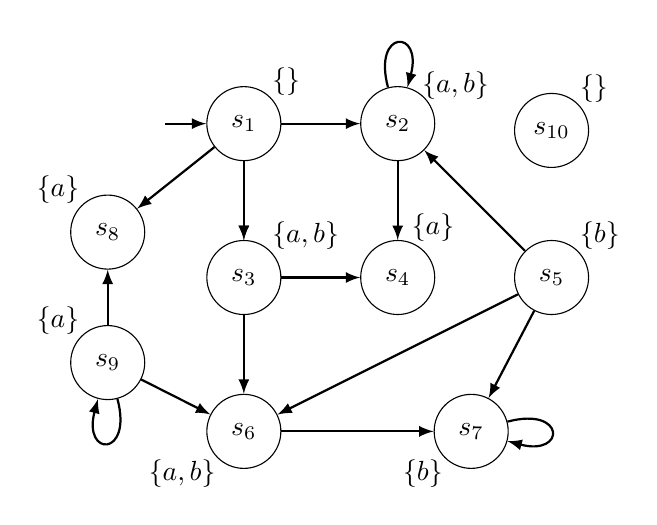
\begin{tikzpicture} [every initial by arrow/.style={thick}]
		%		\createstate{s1}{3,2+4}{$\state_1$};
		\path 
		(\basex,  \basey+2) node[mstate, initial, initial text=, initial distance=15pt] (s1) {$\state_1$} 
		;
		
		\node [mstate,right=of s1] (s2) {$\state_2$};
		\node [mstate,below=of s1] (s3) {$\state_3$};
		\node [mstate,below=of s2] (s4) {$\state_4$};
		\node [mstate,right=of s4] (s5) {$\state_5$};
%		\node [mstate,below right=40pt and 30 pt of s2] (s5) {$\state_5$};
		\node [mstate,below=of s3] (s6) {$\state_6$};
		\node [mstate,right=55pt of s6] (s7) {$\state_7$};
		\node [mstate,below left=20pt and 30pt of s1] (s8) {$\state_8$};
		\node [mstate,below=20pt of s8] (s9) {$\state_9$};
%		\node [mstate,right=of s2] (s10) {$\state_{10}$};
		\node [mstate,above=26pt of s5] (s10) {$\state_{10}$};
		
		\node [above right=-4pt of s1] (ls1) {$\{\}$};
		\node [above right=-6pt of s2] (ls2) {$\{a,b\}$};
		\node [above right=-4pt of s3] (ls3) {$\{a,b\}$};
		\node [above right=0pt and -8pt of s4] (ls4) {$\{a\}$};
		\node [above right=-4pt of s5] (ls5) {$\{b\}$};
		\node [below left=-4pt of s6] (ls6) {$\{a,b\}$};
		\node [below left=-4pt of s7] (ls7) {$\{b\}$};
		\node [above left=-4pt of s8] (ls8) {$\{a\}$};
		\node [above left=-4pt of s9] (ls9) {$\{a\}$};
		\node [above right=-4pt of s10] (ls10) {$\{\}$};
		

		
		
		\path [trans] (s1) edge (s2);
		\path [trans] (s1) edge (s3);
		\path [trans] (s1) edge (s3);
		\path [trans] (s1) edge (s8);
		\path [trans] (s2) edge (s4);
		\path [trans] (s3) edge (s4);
		\path [trans] (s3) edge (s6);
		\path [trans] (s5) edge (s2);
		\path [trans] (s5) edge (s6);
		\path [trans] (s5) edge (s7);
		\path [trans] (s6) edge (s7);
		\path [trans] (s9) edge (s8);
		\path [trans] (s9) edge (s6);
		
		\path [trans] (s2) edge [loop above] (s2);
		\path [trans] (s7) edge [loop right] (s7);
		\path [trans] (s9) edge [loop below] (s9);
		
	\end{tikzpicture}
\end{document}
	\end{minipage}%
	\begin{minipage}{.5\textwidth}
		\documentclass[tikz,preview]{standalone}
%\usepackage{prelude}

%%%%%%%%%%%%%%%%%%%%%%%%%%%%%%%%%%%% PACKAGES %%%%%%%%%%%%%%%%%%%%%%%%%%%%%%%%%%%%%%%%%%

\usepackage{inputenc,fontenc}
\usepackage[a4paper,margin=3cm]{geometry}
\usepackage[english]{babel}
%\usepackage[german]{babel}
%\usepackage[fixlanguage]{babelbib}


\usepackage{bbold}
\usepackage{amsthm}
\usepackage{amsmath}
\usepackage{amssymb} % doteqdot
\usepackage[dvipsnames]{xcolor}
\usepackage{standalone}
\usepackage{tikz}[mode=buildnew]
\usepackage{cite}
\usepackage{xspace}
\usepackage{relsize}
\usepackage{mathtools} % mathclap
%\usepackage{MnSymbol}
\usepackage{hyperref}
\usepackage{url}
\usepackage{listings} % for code
\usepackage[T1]{fontenc} %<
\hypersetup{
	colorlinks,
	citecolor=black,
	filecolor=black,
	linkcolor=black,
	urlcolor=black
}
\usepackage{pgfplots}
\pgfplotsset{compat=1.18}
%\usepackage{courier} %% Sets font for listing as Courier. But also for url and texttt!
\usepackage{listings, xcolor}
\usepackage{graphicx}
\usepackage{subcaption}

\usetikzlibrary{calc}
%\usepackage{xparse} % \newDocumentCommand for multiple optional arguments
%\usepackage{titlecaps}



%%%%%%%%%%%%%%%%%%%%%%%%%%%%%%%%%%%% THEOREMSTYLES %%%%%%%%%%%%%%%%%%%%%%%%%%%%%%%%%%

\theoremstyle{definition}
\newtheorem{definition}{Definition}[section]
\newtheorem{exmp}{Beispiel}[section]
%\AfterEndEnvironment{definition}{\noindent\ignorespaces}

\theoremstyle{theorem}
\newtheorem{theorem}{Satz}[section]
\newtheorem{proposition}{Proposition}[section]
%\AfterEndEnvironment{theorem}{\noindent\ignorespaces}

\theoremstyle{korollary}
\newtheorem{korollary}{Korollar}[section]
%\AfterEndEnvironment{korollary}{\noindent\ignorespaces}


\tikzset{
	mstate/.style={draw, circle, minimum size=.94cm}, 
	gstate/.style={draw, rectangle, minimum size=.8cm},
	varstate/.style={draw,rectangle, rounded corners, minimum size=1}, 
	trans/.style={draw, ->, thick},
	bendtrans/.style={draw, ->, thick, bend left=10},
	bendtransr/.style={draw, ->, thick, bend right=10},
	init/.style={initial, initial distance=6pt, initial text=},
	every loop/.style={min distance=5pt, looseness=8},
	>=latex
}
\usetikzlibrary{automata,positioning}

%auto shift/.style={auto=right,->,
%	to path={ let \p1=(\tikztostart),\p2=(\tikztotarget),
%		\n1={atan2(\y2-\y1,\x2-\x1)},\n2={\n1+180}
%		in ($(\tikztostart.{\n1})!1mm!270:(\tikztotarget.{\n2})$) -- 
%		($(\tikztotarget.{\n2})!1mm!90:(\tikztostart.{\n1})$) \tikztonodes}},

%%%%%%%%%%%%%%%%%%%%%%%%%%%%%%%%%%% MY MACROS %%%%%%%%%%%%%%%%%%%%%%%%%%%%%%%%%%%%%%%%%
%formatting
\newcommand{\comment}[2]{{\color{#1}#2}}
\newcommand{\redcomment}[1]{{\color{red}#1}}
\newcommand{\purpcomment}[1]{{\color{pink}#1}}
\newcommand{\bluecomment}[1]{{\color{blue}#1}}
\newcommand{\mt}[1]{\ensuremath{{#1}}\xspace}
\newcommand{\mynewcommand}[2]{\newcommand{#1}{\mt{#2}}} %% currently not used becaue of ide highlighting
\newcommand{\arr}{\mt{\to}}

%model checking terms
\newcommand{\mimicrel}{\mt{\mathcal{R}}}
\newcommand{\bisimeq}{\mt{\;\!\sim\;\!}}
\newcommand{\simorder}{\mt{\;\!\preceq\;\!}}
\newcommand{\simequiv}{\mt{\;\!\simeq\;\!}} %command already defined
\newcommand{\relts}{\mt{\;\!\bullet_{_{\tiny{TS}}}\;\!}}
\newcommand{\rel}{\mt{\;\!\bullet\;\!}}

%own names
\newcommand{\nm}[1]{#1\xspace}
\newcommand{\mdpN}{\nm{MDP}}
\newcommand{\mdpsN}{\nm{MDPs}}
\newcommand{\viewN}{\nm{view}}
\newcommand{\viewNC}{\nm{View}}
\newcommand{\viewsN}{\nm{views}}
\newcommand{\viewsNC}{\nm{Views}}
\newcommand{\grpfctsubN}{\nm{detached grouping function}}
\newcommand{\grpfctsubNC}{\nm{detached grouping function}}
\newcommand{\grpfctsubNCC}{\nm{Detached Grouping Function}}
\newcommand{\grpfctN}{\nm{grouping function}}
\newcommand{\grpfctNC}{\nm{Grouping function}}
\newcommand{\grpfctNCC}{\nm{Grouping Function}}
\newcommand{\grpfctsN}{\nm{grouping functions}}
\newcommand{\grpfctsNC}{\nm{Grouping functions}}
\newcommand{\grpfctsNCC}{\nm{Grouping Functions}}
\newcommand{\stmimicN}{\nm{state-mimic}}
\newcommand{\stmimicsN}{\nm{state-mimics}}
\newcommand{\stmimickingN}{\nm{state-mimicking}}
\newcommand{\stmimickedN}{\nm{state-mimicked}}
%\newcommand{\chosenphtypeNCC}{\nm{Transition System}}
%\newcommand{\chgphNC}{\nm{Transition system}}
%\newcommand{\chgphN}{\nm{transition system}}
%\newcommand{\chgphsNCC}{\nm{Transition Systems}}
%\newcommand{\chgphsNC}{\nm{Transition systems}}
%\newcommand{\chgphsN}{\nm{transition systems}}
\newcommand{\chgphNCC}{\nm{MDP}}
\newcommand{\chgphNC}{\nm{MDP}}
\newcommand{\chgphN}{\nm{MDP}}
\newcommand{\achgphN}{\nm{an MDP}}
\newcommand{\chgphsNCC}{\nm{MDPs}}
\newcommand{\chgphsNC}{\nm{MDPs}}
\newcommand{\chgphsN}{\nm{MDPs}}
\newcommand{\parllcompN}{\nm{parallel composition}}
\newcommand{\parllcompNC}{\nm{Parallel composition}}
\newcommand{\parllcompNCC}{\nm{Parallel Composition}}
\newcommand{\parllcompsN}{\nm{parallel compositions}}
\newcommand{\parllcompsNC}{\nm{Parallel compositions}}
\newcommand{\parllcompsNCC}{\nm{Parallel Compositions}}
\newcommand{\sccN}{\nm{SCC}}
\newcommand{\sccsN}{\nm{SCCs}}
\newcommand{\bsccN}{\nm{BSCC}}
\newcommand{\bsccsN}{\nm{BSCCs}}
\newcommand{\jgrapht}{\nm{jGraphtT}}

\newcommand{\outactident}{\nm{OutActionsIdent}}

%names
\newcommand{\iffN}{\nm{if and only if}}
\newcommand{\tsN}{\nm{TS}}

%% outactions identical
\newcommand{\outactidentstrong}{\nm{strong}}
\newcommand{\outactidentweak}{\nm{weak}}

% CORE DEFINITIONS
\newcommand{\grpfct}[1][\viewppty]{\mt{F_{#1}}}
\newcommand{\grpfctsub}[1][\viewppty]{\mt{\tilde{F}_{#1}}}
%\newcommand{\grpfctimg}[1]{\mt{{\grpfct}[{#1}]}}
%\newcommand{\fctimg}[2]{\mt{{#1}[{#2}]}}
\newcommand{\eqrelview}{\mt{R}}
\newcommand{\eqclassv}[1][\state]{\mt{\eqclass{#1}{\eqrelview}}}
\newcommand{\eqclasssetv}[1][\states]{\mt{{#1}/\eqrelview}} %OLD: \bigcup_{\state \in \states} \eqclassv
\newcommand{\viewid}{\mt{\mdp}}
\newcommand{\view}[1][\viewppty]{\mt{\viewid_{#1}}}
\newcommand{\imggrp}{\mt{\arbset}}
\newcommand{\imggrpsub}{\mt{X}}
\newcommand{\viewppty}{\mt{\theta}}
\newcommand{\pll}{\mt{\;\!\pllpure\;\!}}
\newcommand{\pllrev}{\mt{\pllpure^{-1}}}
\newcommand{\pllpure}{\mt{||}}
\newcommand{\compselectset}{\mt{Z}}
\newcommand{\compselectpure}{\mt{\pllpure_\compselectset}}
\newcommand{\compselect}{\mt{\;\pllpure_\compselectset\;}}
\newcommand{\remstates}{\mt{\bigcup_{\state \in \states \setminus \states_1}\{\{\state\}\}}}
\newcommand{\nogroupstates}[1][\states_2]{\mt{\bigcup_{\state \in \states \setminus {#1}}\{\{\state\}\}}}
\newcommand{\remelem}{\mt{\bullet}}
\newcommand{\nogroupset}{\mt{\xi}}
\newcommand{\remset}{\mt{\{\remelem\}}}
\newcommand{\gfctpll}{\mt{\grpfct[\pll]}}
\newcommand{\group}{\mt{\top}}
\newcommand{\imggrpbinview}{\mt{\{\remelem, \notppty\}}}
\newcommand{\viewappset}{\mt{\tilde{\states}}}
\newcommand{\hasppty}{\mt{\top}}
\newcommand{\notppty}{\mt{\bot}}
\newcommand{\disregardelem}{\mt{\Delta}}
\newcommand{\disregardelements}{\mt{{\disregardelem_1, \dots, \disregardelem_n}}}



%\newcommand{\mdp}{def}\mdp
%\newcommand{\mdpdef}



% EXAMPLE VIEWS
\newcommand{\pptyatomicprops}{\mt{\atomicprops}}
\newcommand{\pptyinitstates}{\mt{\initstates}}
\newcommand{\pptyinactsetsize}{\mt{|\inacts(\state)|}}
\newcommand{\pptyhasoutact}{\mt{\exists\outact}}
\newcommand{\pptyminoutact}[2]{\mt{#1\leq#2}}
\newcommand{\pptymaxoutact}[2]{\mt{#2\leq#1}}
\newcommand{\pptyspanoutact}[3]{\mt{#1\leq#2\leq#3}}
\newcommand{\pptyoutactsetsize}{\mt{|\outacts(\state)|}}
\newcommand{\pptyoutactsingle}{\mt{|\outacts(\state)|_1}}
\newcommand{\pptystrongoutactident}{\mt{\outacts(\state)_=}}
\newcommand{\pptyweakoutactident}{\mt{\outacts(\state)_\approx}}
\newcommand{\pptyhasinact}{\mt{\exists\inact}}
\newcommand{\pptymininact}[2]{\mt{#1\leq#2}}
\newcommand{\pptymaxinact}[2]{\mt{#2\leq#1}}
\newcommand{\pptyspaninact}[3]{\mt{#1\leq#2\leq#3}}
\newcommand{\pptyinactsingle}{\mt{|\inacts(\state)|_1}}
\newcommand{\pptystronginactident}{\mt{\inacts(\state)_=}}
\newcommand{\pptyweakinactident}{\mt{\inacts(\state)_\approx}}
\newcommand{\pptyparamvalueseq}{\mt{\var = \varval}}
\newcommand{\pptyparamvaluesneq}{\mt{\var \neq \varval}}
\newcommand{\pptyparamdnf}{\mt{VarDNF}}
\newcommand{\pptyparamcnf}{\mt{VarCNF}}
\newcommand{\pptyparamvalueseqopt}{\mt{\var = \varval}}
\newcommand{\pptyparamvalident}{\mt{Var:\varval}}
\newcommand{\pptydistance}{\mt{\distpath}}
\newcommand{\pptydistancerev}{\mt{\distpathrev}}
\newcommand{\pptydistancebi}{\mt{\distpathbi}}
\newcommand{\pptyhascycle}{\mt{\exists\cycle}}
\newcommand{\pptyexactactcycle}{\mt{\{\cycle_{\action,n}\}}}
\newcommand{\pptycycleset}{\mt{\cup{\{\state\}_\cycle}}}
\newcommand{\pptyexactcycle}{\mt{\{\cycle_n\}}}
\newcommand{\pptyscc}{\mt{scc}}
\newcommand{\pptybscc}{\mt{bscc}}
\newcommand{\pptyprop}{\mt{\redcomment{?}}}
\newcommand{\pptyident}{id}


\newcommand{\gfctatomicprops}{\mt{\grpfct[\pptyatomicprops]}}
\newcommand{\gfctinitstates}{\mt{\grpfct[\pptyinitstates]^\hasppty}}
\newcommand{\gfcthasoutaction}{\mt{\grpfct[\pptyhasoutact]^\hasppty}}
\newcommand{\gfctminoutaction}{\mt{\grpfct[\pptyminoutact{\numoutact}{\outact}]^\hasppty}}
\newcommand{\gfctmaxoutaction}{\mt{\grpfct[\pptymaxoutact{\numoutact}{\outact}]^\hasppty}}
\newcommand{\gfctspanoutaction}{\mt{\grpfct[\pptyspanoutact{\numoutactb}{\outact}{\numoutact}]^\hasppty}}
\newcommand{\gfctoutactsetsize}{\mt{\grpfct[\pptyoutactsetsize]}}
\newcommand{\gfctoutactsingle}{\mt{\grpfct[\pptyoutactsingle]^\notppty}}
\newcommand{\gfctstrongoutactident}{\mt{\grpfct[\pptystrongoutactident]}}
\newcommand{\gfctweakoutactident}{\mt{\grpfct[\pptyweakoutactident]}}
\newcommand{\gfcthasinaction}{\mt{\grpfct[\pptyhasinact]^\hasppty}}
\newcommand{\gfctmininaction}{\mt{\grpfct[\pptymininact{\numinact}{\inact}]^\hasppty}}
\newcommand{\gfctmaxinaction}{\mt{\grpfct[\pptymaxinact{\numinact}{\inact}]^\hasppty}}
\newcommand{\gfctspaninaction}{\mt{\grpfct[\pptyspaninact{\numinactb}{\inact}{\numinact}]^\hasppty}}
\newcommand{\gfctinactsetsize}{\mt{\grpfct[\pptyinactsetsize]}}
\newcommand{\gfctinactsingle}{\mt{\grpfct[\pptyinactsingle]^\notppty}}
\newcommand{\gfctstronginactident}{\mt{\grpfct[\pptystronginactident]}}
\newcommand{\gfctweakinactident}{\mt{\grpfct[\pptyweakinactident]}}
\newcommand{\gfctparamvalueseq}{\mt{\grpfct[\pptyparamvalueseq]^\hasppty}}
\newcommand{\gfctparamvaluesneq}{\mt{\grpfct[\pptyparamvaluesneq]^\hasppty}}
\newcommand{\gfctparamdnf}{\mt{\grpfct[\pptyparamdnf]^\hasppty}}
\newcommand{\gfctparamcnf}{\mt{\grpfct[\pptyparamcnf]^\hasppty}}
\newcommand{\gfctparamvalueseqopt}{\mt{\pptyparamvalueseqopt}}
\newcommand{\gfctparamvalident}{\mt{\grpfct[\pptyparamvalident]}}
\newcommand{\gfctdistance}{\mt{\grpfct[\pptydistance]}}
\newcommand{\gfctdistancerev}{\mt{\grpfct[\pptydistancerev]}}
\newcommand{\gfctdistancebi}{\mt{\grpfct[\pptydistancebi]}}
\newcommand{\gfcthascycle}{\mt{\grpfct[\pptyhascycle]}}
\newcommand{\gfctexactcycle}{\mt{\grpfct[\pptyexactcycle]}}
\newcommand{\gfctcycleset}{\mt{\grpfct[\pptycycleset]}}
\newcommand{\gfctexactactcycle}{\mt{\grpfct[\pptyexactactcycle]}}
\newcommand{\gfctscc}{\mt{\grpfct[\pptyscc]}}
\newcommand{\gfctbscc}{\mt{\grpfct[\pptybscc]}}
\newcommand{\gfctprop}{\mt{\grpfct[\pptyprop]}}
\newcommand{\gfctident}{\mt{\grpfct[\pptyident]}}

\newcommand{\gfctsubatomicprops}{\mt{\grpfctsub[\pptyatomicprops]}}
\newcommand{\gfctsubinitstates}{\mt{\grpfctsub[\pptyinitstates]^\hasppty}}
\newcommand{\gfctsubhasoutaction}{\mt{\grpfctsub[\pptyhasoutact]^\hasppty}}
\newcommand{\gfctsubminoutaction}{\mt{\grpfctsub[\pptyminoutact{\numoutact}{\outact}]^\hasppty}}
\newcommand{\gfctsubmaxoutaction}{\mt{\grpfctsub[\pptymaxoutact{\numoutact}{\outact}]^\hasppty}}
\newcommand{\gfctsubspanoutaction}{\mt{\grpfctsub[\pptyspanoutact{\numoutactb}{\outact}{\numoutact}]^\hasppty}}
\newcommand{\gfctsuboutactsetsize}{\mt{\grpfctsub[\pptyoutactsetsize]}}
\newcommand{\gfctsuboutactsingle}{\mt{\grpfctsub[\pptyoutactsingle]^\notppty}}
\newcommand{\gfctsubstrongoutactident}{\mt{\grpfctsub[\pptystrongoutactident]^\hasppty}}
\newcommand{\gfctsubweakoutactident}{\mt{\grpfctsub[\pptyweakoutactident]^\hasppty}}
\newcommand{\gfctsubhasinaction}{\mt{\grpfctsub[\pptyhasinact]}}
\newcommand{\gfctsubmininaction}{\mt{\grpfctsub[\pptymininact{\numinact}{\inact}]}}
\newcommand{\gfctsubmaxinaction}{\mt{\grpfctsub[\pptymaxinact{\numinact}{\inact}]}}
\newcommand{\gfctsubspaninaction}{\mt{\grpfctsub[\pptyspaninact{\numinactb}{\inact}{\numinact}]}}
\newcommand{\gfctsubinactsetsize}{\mt{\grpfctsub[\pptyinactsetsize]^\hasppty}}
\newcommand{\gfctsubinactsingle}{\mt{\grpfctsub[\pptyinactsingle]^\notppty}}
\newcommand{\gfctsubstronginactident}{\mt{\grpfctsub[\pptystronginactident]}}
\newcommand{\gfctsubweakinactident}{\mt{\grpfctsub[\pptyweakinactident]}}
\newcommand{\gfctsubparamvalueseq}{\mt{\grpfctsub[\pptyparamvalueseq]^\hasppty}}
\newcommand{\gfctsubparamvaluesneq}{\mt{\grpfctsub[\pptyparamvaluesneq]^\hasppty}}
\newcommand{\gfctsubparamdnf}{\mt{\grpfctsub[\pptyparamdnf]^\hasppty}}
\newcommand{\gfctsubparamcnf}{\mt{\grpfctsub[\pptyparamcnf]^\hasppty}}
\newcommand{\gfctsubparamvalueseqopt}{\mt{\pptyparamvalueseqopt}}
\newcommand{\gfctsubparamvalident}{\mt{\grpfctsub[\pptyparamvalident]}}
\newcommand{\gfctsubdistance}{\mt{\grpfctsub[\pptydistance]}}
\newcommand{\gfctsubdistancerev}{\mt{\grpfctsub[\pptydistancerev]}}
\newcommand{\gfctsubdistancebi}{\mt{\grpfctsub[\pptydistancebi]}}
\newcommand{\gfctsubhascycle}{\mt{\grpfctsub[\pptyhascycle]^\hasppty}}
\newcommand{\gfctsubexactcycle}{\mt{\grpfctsub[\pptyexactcycle]}}
\newcommand{\gfctsubcycleset}{\mt{\grpfctsub[\pptycycleset]}}
\newcommand{\gfctsubexactactcycle}{\mt{\grpfctsub[\pptyexactactcycle]}}
\newcommand{\gfctsubscc}{\mt{\grpfctsub[\pptyscc]}}
\newcommand{\gfctsubbscc}{\mt{\grpfctsub[\pptybscc]}}
\newcommand{\gfctsubprop}{\mt{\grpfctsub[\pptyprop]}}
\newcommand{\gfctsubident}{\mt{\grpfctsub[\pptyident]}}


\newcommand{\viewatomicprops}{\mt{\view[\pptyatomicprops]}}
\newcommand{\viewinitstates}{\mt{\view[\pptyinitstates]^\hasppty}}
\newcommand{\viewhasoutaction}{\mt{\view[\pptyhasoutact]^\hasppty}}
\newcommand{\viewminoutaction}{\mt{\view[\pptyminoutact{\numoutact}{\outact}]^\hasppty}}
\newcommand{\viewmaxoutaction}{\mt{\view[\pptymaxoutact{\numoutact}{\outact}]^\hasppty}}
\newcommand{\viewspanoutaction}{\mt{\view[\pptyspanoutact{\numoutactb}{\outact}{\numoutact}]^\hasppty}}
\newcommand{\viewoutactsetsize}{\mt{\view[\pptyoutactsetsize]}}
\newcommand{\viewoutactsingle}{\mt{\view[\pptyoutactsingle]^\notppty}}
\newcommand{\viewstrongoutactident}{\mt{\view[\pptystrongoutactident]}}
\newcommand{\viewweakoutactident}{\mt{\view[\pptyweakoutactident]}}
\newcommand{\viewhasinaction}{\mt{\view[\pptyhasinact]^\hasppty}}
\newcommand{\viewmininaction}{\mt{\view[\pptymininact{\numinact}{\inact}]^\hasppty}}
\newcommand{\viewmaxinaction}{\mt{\view[\pptymaxinact{\numinact}{\inact}]^\hasppty}}
\newcommand{\viewspaninaction}{\mt{\view[\pptyspaninact{\numinactb}{\inact}{\numinact}]^\hasppty}}
\newcommand{\viewinactsetsize}{\mt{\view[\pptyinactsetsize]}}
\newcommand{\viewinactsingle}{\mt{\view[\pptyinactsingle]^\notppty}}
\newcommand{\viewstronginactident}{\mt{\view[\pptystronginactident]}}
\newcommand{\viewweakinactident}{\mt{\view[\pptyweakinactident]}}
\newcommand{\viewparamvalueseq}{\mt{\view[\pptyparamvalueseq]}}
\newcommand{\viewparamvaluesneq}{\mt{\view[\pptyparamvaluesneq]}}
\newcommand{\viewparamdnf}{\mt{\view[\pptyparamdnf]^\hasppty}}
\newcommand{\viewparamcnf}{\mt{\view[\pptyparamcnf]^\hasppty}}
\newcommand{\viewparamvalueseqopt}{\mt{\pptyparamvalueseqopt}}
\newcommand{\viewparamvalident}{\mt{\view[\pptyparamvalident]}}
\newcommand{\viewdistance}{\mt{\view[\pptydistance]}}
\newcommand{\viewdistancerev}{\mt{\view[\pptydistancerev]}}
\newcommand{\viewdistancebi}{\mt{\view[\pptydistancebi]}}
\newcommand{\viewhascycle}{\mt{\view[\pptyhascycle]}}
\newcommand{\viewexactcycle}{\mt{\view[\pptyexactcycle]}}
\newcommand{\viewcycleset}{\mt{\view[\pptycycleset]}}
\newcommand{\viewexactactcycle}{\mt{\view[\pptyexactactcycle]}}
\newcommand{\viewscc}{\mt{\view[\pptyscc]}}
\newcommand{\viewbscc}{\mt{\view[\pptybscc]}}
\newcommand{\viewprop}{\mt{\view[\pptyprop]}}
\newcommand{\viewident}{\mt{\view[\pptyident]}}

%\newcommand{\viewatomicprops}{\mt{\view[\atomicprops]}}
%\newcommand{\viewinitstates}{\mt{\view[\initstates]}}
%\newcommand{\viewhasoutaction}{\mt{\view[\pptyhasoutact]}}
%\newcommand{\viewminoutaction}{\mt{\view[\pptyminoutact{\numoutact}{\outact}]}}
%\newcommand{\viewmaxoutaction}{\mt{\view[\pptymaxoutact{\numoutact}{\outact}]}}
%\newcommand{\viewspanoutaction}{\mt{\view[\pptyspanoutact{\numoutactb}{\outact}{\numoutact}]}}
%\newcommand{\viewoutactsetsize}{\mt{\view[\pptyoutactsetsize]}}
%\newcommand{\viewoutactsingle}{\mt{\view[\pptyoutactsingle]}}
%\newcommand{\viewstrongoutactident}{\mt{\view[\outacts(\state)_=]}}
%\newcommand{\viewweakoutactident}{\mt{\view[\outacts(\state)_\approx]}}
%\newcommand{\viewhasinaction}{\mt{\view[\pptyhasinact]}}
%\newcommand{\viewmininaction}{\mt{\view[\pptymininact{\numinact}{\inact}]}}
%\newcommand{\viewmaxinaction}{\mt{\view[\pptymaxinact{\numinact}{\inact}]}}
%\newcommand{\viewspaninaction}{\mt{\view[\pptyspaninact{\numinactb}{\inact}{\numinact}]}}
%\newcommand{\viewinactsetsize}{\mt{\view[\pptyinactsetsize]}}
%\newcommand{\viewinactsingle}{\mt{\view[\pptyinactsingle]}}
%\newcommand{\viewstronginactident}{\mt{\view[\inacts(\state)_=]}}
%\newcommand{\viewweakinactident}{\mt{\view[\inacts(\state)_\approx]}}
%\newcommand{\viewparamvalueseq}{\mt{\view[\var = \varval]}}
%\newcommand{\viewparamvaluesneq}{\mt{\view[\var \neq \varval]}}
%\newcommand{\viewparamdnf}{\mt{\view[VarDNF]}}
%\newcommand{\viewparamcnf}{\mt{\view[VarCNF]}}
%\newcommand{\viewparamvalident}{\mt{\view[\pptyparamvalident]}}
%\newcommand{\viewdistance}{\mt{\view[\pptydistance]}}
%\newcommand{\viewhascycle}{\mt{\view[\exists\cycle]}}
%\newcommand{\viewexactcycle}{\mt{\view[\pptyexactcycle]}}
%\newcommand{\viewcycleset}{\mt{\view[\pptycycleset]}}
%\newcommand{\viewexactactcycle}{\mt{\view[\pptyexactactcycle]}}
%\newcommand{\viewscc}{\mt{\view[scc]}}
%\newcommand{\viewbscc}{\mt{\view[bscc]}}

%actions
\newcommand{\numoutact}{\mt{n}}
\newcommand{\numoutactb}{\mt{m}}
\newcommand{\numinact}{\mt{n}}
\newcommand{\numinactb}{\mt{m}}

\newcommand{\predmaxoutact}[1][\numoutact]{\mt{Q_{\outact\leq#1}(\state,\state_1, \dots, \state_{#1+1})}}
\newcommand{\predminoutact}[1][\numoutact]{\mt{Q_{#1\leq\outact}(\state,\state_1, \dots, \state_{#1})}}
\newcommand{\formoutact}[1][\state]{\mt{C_{#1,\outact}}}
\newcommand{\predmaxinact}[1][\numinact]{\mt{Q_{\inact\leq#1}(\state,\state_1, \dots, \state_{#1+1})}}
\newcommand{\predmininact}[1][\numinact]{\mt{Q_{#1\leq\inact}(\state,\state_1, \dots, \state_{#1})}}

\newcommand{\outact}[1][\action]{\mt{\overrightarrow{#1}}}
\newcommand{\outacts}{\mt{\overrightarrow{\actions}}}
\newcommand{\inact}{\mt{\overleftarrow{\action}}}
\newcommand{\inacts}[1][\action]{\mt{\overleftarrow{#1}}}

%%Parameters
\newcommand{\vars}[1][\mdp]{\mt{V\!ar_{#1}}}
\newcommand{\var}{\mt{x}}
\newcommand{\varstate}[1][]{\mt{\var_{\state#1}}}
\newcommand{\varval}{\mt{a}}
\newcommand{\vareval}[1][\mdp]{\mt{V\!arEval_{#1}}}
\newcommand{\varevalimg}[1][\mdp]{\mt{\vareval[#1][\states,\vars]}}
\newcommand{\varevalimgset}{\mt{\arbset}}
\newcommand{\someparam}{\mt{\tilde{x}}}
\newcommand{\eqorneq}{\mt{\;\doteqdot\;}}
\newcommand{\varstyle}[2]{\mt{\langle#1,#2\rangle}}




%\makeatletter
%\newcommand{\overleftrightsmallarrow}{\mathpalette{\overarrowsmall@\leftrightarrowfill@}}
%\newcommand{\overrightsmallarrow}{\mathpalette{\overarrowsmall@\rightarrowfill@}}
%\newcommand{\overleftsmallarrow}{\mathpalette{\overarrowsmall@\leftarrowfill@}}
%\newcommand{\overarrowsmall@}[3]{%
%	\vbox{%
%		\ialign{%
%			##\crcr
%			#1{\smaller@style{#2}}\crcr
%			\noalign{\nointerlineskip}%
%			$\m@th\hfil#2#3\hfil$\crcr
%		}%
%	}%
%}
%\def\smaller@style#1{%
%	\ifx#1\displaystyle\scriptstyle\else
%	\ifx#1\textstyle\scriptstyle\else
%	\scriptscriptstyle
%	\fi
%	\fi
%}
%\makeatother
%\newcommand{\te}[1]{\overleftrightsmallarrow{#1}}

% Distance
\newcommand{\fctdist}{\mt{distance}}
\newcommand{\fctdistdefault}{\mt{\fctdist(\chgph, \smstates, \grandist)}}
\newcommand{\distval}{\mt{d}}
\newcommand{\grandist}{\mt{n}}
\let\path\oldpath
\newcommand{\path}{\mt{P}}
\newcommand{\pathbi}{\mt{\bar{\path}}}
\newcommand{\pathsecfull}{\mt{(\state_0, \action_0, \state_1, \action_1, \dots, \action_{n}, \state_{n+1})}}
\newcommand{\lenpath}{\mt{len}}
\newcommand{\pfirst}{\mt{first}}
\newcommand{\plast}{\mt{last}}
\newcommand{\pathset}{\mt{\path_\chgph}}
\newcommand{\pathbiset}{\mt{\pathbi_\chgph}}
\newcommand{\distpath}{\mt{\overrightarrow{dist}}}
\newcommand{\distpathrev}{\mt{\overleftarrow{dist}}}
\newcommand{\distpathbi}{\mt{\overline{dist}}}
%Cycles
\newcommand{\cyclesecfull}{\mt{(\state_0, \action_0, \state_1, \action_1, \dots, \action_{n-1}, \state_0)}}
\newcommand{\fctfindcycles}{\mt{findCycles}}
\newcommand{\cycle}{\mt{C}}
\newcommand{\cycleset}{\mt{\cycle_{\mdp, n}}}
\newcommand{\lencycle}{\mt{len}}
% strongly connected components
\newcommand{\scc}{\mt{T}}
\newcommand{\setscc}{\mt{SCC_{\chgph,n}}}
\newcommand{\setbscc}{\mt{BSCC_{\chgph,n}}}

% properties
\newcommand{\propfct}{\mt{f}}

% all Systems
\newcommand{\chgph}{\mt{\mdp}}
\newcommand{\chgphtuple}{\mt{\mdptuple}}
\newcommand{\chgphtupledist}{\mt{\mdptupledist}}

\newcommand{\states}{\mt{S}}
\newcommand{\actions}{\mt{Act}}
\newcommand{\atomicprops}{\mt{AP}}
\newcommand{\labelingfct}{\mt{L}}
\newcommand{\init}{\mt{\initdistrib}} % use MDP % refers to the underlying set
\newcommand{\trans}{\mt{\probtfunc}} % use MDP % refers to the underlying set
\newcommand{\smstates}{\mt{\tilde{\states}}}


\newcommand{\state}{\mt{s}}
\newcommand{\action}{\mt{\alpha}}
\newcommand{\actionb}{\mt{\beta}}
\newcommand{\actionc}{\mt{\gamma}}
\newcommand{\smstate}{\mt{\tilde{\state}}}



% transition sysstems
\newcommand{\ts}{\mt{TS}}
\newcommand{\transitionrel}{\mt{\longrightarrow}}
\newcommand{\initstates}{\mt{I}}
\newcommand{\transitionsystem}{\mt
	{(\states, \actions, \transitionrel, \initstates, \atomicprops, \labelingfct)}
}
\newcommand{\tstupledist}{\mt{(\states', \actions',\transitionrel', \initstates', \labelingfct')}}


%Markov chains and MDP
\newcommand{\mdp}{\mt{\autm}}
\newcommand{\mdptuple}{\mt{(\states, \actions, \probtfunc, \initdistrib, \atomicprops, \labelingfct)}}
\newcommand{\mdptupledist}{\mt{(\states', \actions', \probtfunc', \initdistrib', \atomicprops', \labelingfct')}}
\newcommand{\autm}{\mt{\mathcal{M}}}
\newcommand{\probtfunc}{\mt{\textbf{P}}}
\newcommand{\initdistrib}{\mt{\iota_{init}}}


%maths
\newcommand{\powerset}[1]{\mt{\mathcal{P}(#1)}}
\newcommand{\eqclass}[2]{\mt{[#1]_{#2}}}%{\mt{#1 / #2}}
\newcommand{\impr}{\mt{\hspace{3mm}\Rightarrow\hspace{2mm}}}
\newcommand{\impl}{\mt{\hspace{3mm}\Leftarrow\hspace{2mm}}}
\newcommand{\natnums}{\mt{\mathbb{N}}} 
\newcommand{\realnums}{\mt{\mathbb{R}}}
\newcommand{\intmodn}[1][n]{\mt{\mathbb{Z}_{#1}}}
\newcommand{\arbset}{\mt{M}}
\newcommand{\bigsum}[2][]{\mt{\mathlarger{\sum}_{#2}^{#1}}}
\newcommand{\bbigsum}[2][]{\mt{\mathlarger{\mathlarger{\sum}}_{#2}^{#1}}}
\newcommand{\invimage}[2]{#1^{\mt{-1}(#2)}}
\newcommand{\img}{\mt{Img}}
\newcommand{\cond}{\mt{\,|\,}}

%tickz
%% \definecolor{darkred}{RGB}{196, 42, 42}

%implementation
\newcommand{\pmcvis}{\nm{PMC-Vis}}





\begin{document}
	\newcommand{\basex}{0}
	\newcommand{\basey}{-.4}
	\newcommand{\createstate}[3]{\node[draw, circle, minimum size=1cm] (#1) at (#2) {#3}}
	
	
	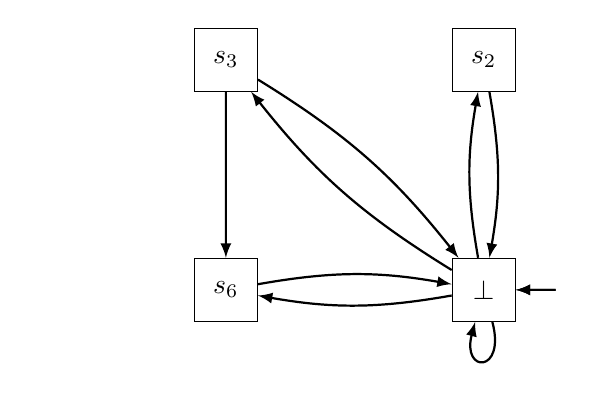
\begin{tikzpicture} [scale=2.4, every initial by arrow/.style={thick}]
		
		\newcommand{\disth}{70pt}
		\newcommand{\distv}{60pt}
		
		\node at (0,0) {};
		
		\node [gstate] (s3) at (\basex,\basey) {$\state_3$};
		\node [gstate,right=\disth of s3] (s2) {$\state_2$};
		\node [gstate,below=\distv of s3] (s6) {$\state_6$};
		\node [gstate,init,initial right,below=\distv of s2] (sbot) {$\notppty$};
		
		\path [trans] (s3) edge (s6);

		\path [bendtrans] (s2) edge (sbot);
		\path [bendtrans] (s3) edge (sbot);
		\path [bendtrans] (s6) edge (sbot);
		\path [bendtrans] (sbot) edge (s2);
		\path [bendtrans] (sbot) edge (s3);
		\path [bendtrans] (sbot) edge (s6);
		
		\path [trans] (sbot) edge [loop below] (sbot);
	
		
		
		%		midway, at start, near start, very near start, at end, near end, very near end
		
		
	\end{tikzpicture}
\end{document}
	\end{minipage}
	\caption{Simplified representations of \mdp (left) and the \viewN \viewatomicprops on it (right)}
	\label{fig:apHasBeforeAfter}  
\end{figure}


\begin{definition}	
	Let $\chgph = \chgphtuple$ be \achgphN. The view \viewatomicprops is defined by its grouping function \gfctatomicprops \grpfctN with $\gfctatomicprops : \states \to \imggrp, {\state}\mapsto{\labelingfct(\state)}$.
\end{definition}

The grouping function is exactly the labeling function i.e. for all $\state \in \states$ it is $\gfctatomicprops(\state) := \labelingfct(\state)$. So it is $\gfctatomicprops(\state_1) = \gfctatomicprops(\state_2) \iff \labelingfct(\state_1) = \labelingfct(\state_2)$. According to Definition \ref{def:eqrelview} for $\smstate \in \states$ it is $\eqclassv[\smstate] = \{\state \in \states \mid \labelingfct(\state) = \labelingfct(\smstate)\}$.
%$\forall \state_1, \state_2 \in \states :

By this we obtain the \viewN $\viewatomicprops$ for a given \chgphN \chgph where: $\states' = \bigcup_{\state \in \states} \{\eqclassv\} =  \bigcup_{a \in \atomicprops} \{\{\state \in \states \mid \labelingfct(\state) = a\}\}$. All other components are constructed as in Definition \ref{def:view}.

Although this view might seem rather simple because essentially it only performs $\gfctatomicprops := \labelingfct$ it is the most powerful one. This is because every view presented in the following is reducible to this one. That is because a \grpfctN essentially asserts an atomic proposition to every state, namely the value in respect to the considered property of a given view. The reduction can be realized by replacing the labeling function with the grouping function of the resepective view. That is $\labelingfct := \grpfct$ and $\atomicprops := \redcomment{\grpfct(\states)}$ for some \grpfctN \grpfct. While this works it alters the underlying \chgphN.

\begin{figure}[h]
	\begin{minipage}{.6\textwidth}
%		\hspace{5mm}
		\documentclass[tikz]{standalone}
%\usepackage{prelude}

%%%%%%%%%%%%%%%%%%%%%%%%%%%%%%%%%%%% PACKAGES %%%%%%%%%%%%%%%%%%%%%%%%%%%%%%%%%%%%%%%%%%

\usepackage{inputenc,fontenc}
\usepackage[a4paper,margin=3cm]{geometry}
\usepackage[english]{babel}
%\usepackage[german]{babel}
%\usepackage[fixlanguage]{babelbib}


\usepackage{bbold}
\usepackage{amsthm}
\usepackage{amsmath}
\usepackage{amssymb} % doteqdot
\usepackage[dvipsnames]{xcolor}
\usepackage{standalone}
\usepackage{tikz}[mode=buildnew]
\usepackage{cite}
\usepackage{xspace}
\usepackage{relsize}
\usepackage{mathtools} % mathclap
%\usepackage{MnSymbol}
\usepackage{hyperref}
\usepackage{url}
\usepackage{listings} % for code
\usepackage[T1]{fontenc} %<
\hypersetup{
	colorlinks,
	citecolor=black,
	filecolor=black,
	linkcolor=black,
	urlcolor=black
}
\usepackage{pgfplots}
\pgfplotsset{compat=1.18}
%\usepackage{courier} %% Sets font for listing as Courier. But also for url and texttt!
\usepackage{listings, xcolor}
\usepackage{graphicx}
\usepackage{subcaption}

\usetikzlibrary{calc}
%\usepackage{xparse} % \newDocumentCommand for multiple optional arguments
%\usepackage{titlecaps}



%%%%%%%%%%%%%%%%%%%%%%%%%%%%%%%%%%%% THEOREMSTYLES %%%%%%%%%%%%%%%%%%%%%%%%%%%%%%%%%%

\theoremstyle{definition}
\newtheorem{definition}{Definition}[section]
\newtheorem{exmp}{Beispiel}[section]
%\AfterEndEnvironment{definition}{\noindent\ignorespaces}

\theoremstyle{theorem}
\newtheorem{theorem}{Satz}[section]
\newtheorem{proposition}{Proposition}[section]
%\AfterEndEnvironment{theorem}{\noindent\ignorespaces}

\theoremstyle{korollary}
\newtheorem{korollary}{Korollar}[section]
%\AfterEndEnvironment{korollary}{\noindent\ignorespaces}


\tikzset{
	mstate/.style={draw, circle, minimum size=.94cm}, 
	gstate/.style={draw, rectangle, minimum size=.8cm},
	varstate/.style={draw,rectangle, rounded corners, minimum size=1}, 
	trans/.style={draw, ->, thick},
	bendtrans/.style={draw, ->, thick, bend left=10},
	bendtransr/.style={draw, ->, thick, bend right=10},
	init/.style={initial, initial distance=6pt, initial text=},
	every loop/.style={min distance=5pt, looseness=8},
	>=latex
}
\usetikzlibrary{automata,positioning}

%auto shift/.style={auto=right,->,
%	to path={ let \p1=(\tikztostart),\p2=(\tikztotarget),
%		\n1={atan2(\y2-\y1,\x2-\x1)},\n2={\n1+180}
%		in ($(\tikztostart.{\n1})!1mm!270:(\tikztotarget.{\n2})$) -- 
%		($(\tikztotarget.{\n2})!1mm!90:(\tikztostart.{\n1})$) \tikztonodes}},

%%%%%%%%%%%%%%%%%%%%%%%%%%%%%%%%%%% MY MACROS %%%%%%%%%%%%%%%%%%%%%%%%%%%%%%%%%%%%%%%%%
%formatting
\newcommand{\comment}[2]{{\color{#1}#2}}
\newcommand{\redcomment}[1]{{\color{red}#1}}
\newcommand{\purpcomment}[1]{{\color{pink}#1}}
\newcommand{\bluecomment}[1]{{\color{blue}#1}}
\newcommand{\mt}[1]{\ensuremath{{#1}}\xspace}
\newcommand{\mynewcommand}[2]{\newcommand{#1}{\mt{#2}}} %% currently not used becaue of ide highlighting
\newcommand{\arr}{\mt{\to}}

%model checking terms
\newcommand{\mimicrel}{\mt{\mathcal{R}}}
\newcommand{\bisimeq}{\mt{\;\!\sim\;\!}}
\newcommand{\simorder}{\mt{\;\!\preceq\;\!}}
\newcommand{\simequiv}{\mt{\;\!\simeq\;\!}} %command already defined
\newcommand{\relts}{\mt{\;\!\bullet_{_{\tiny{TS}}}\;\!}}
\newcommand{\rel}{\mt{\;\!\bullet\;\!}}

%own names
\newcommand{\nm}[1]{#1\xspace}
\newcommand{\mdpN}{\nm{MDP}}
\newcommand{\mdpsN}{\nm{MDPs}}
\newcommand{\viewN}{\nm{view}}
\newcommand{\viewNC}{\nm{View}}
\newcommand{\viewsN}{\nm{views}}
\newcommand{\viewsNC}{\nm{Views}}
\newcommand{\grpfctsubN}{\nm{detached grouping function}}
\newcommand{\grpfctsubNC}{\nm{detached grouping function}}
\newcommand{\grpfctsubNCC}{\nm{Detached Grouping Function}}
\newcommand{\grpfctN}{\nm{grouping function}}
\newcommand{\grpfctNC}{\nm{Grouping function}}
\newcommand{\grpfctNCC}{\nm{Grouping Function}}
\newcommand{\grpfctsN}{\nm{grouping functions}}
\newcommand{\grpfctsNC}{\nm{Grouping functions}}
\newcommand{\grpfctsNCC}{\nm{Grouping Functions}}
\newcommand{\stmimicN}{\nm{state-mimic}}
\newcommand{\stmimicsN}{\nm{state-mimics}}
\newcommand{\stmimickingN}{\nm{state-mimicking}}
\newcommand{\stmimickedN}{\nm{state-mimicked}}
%\newcommand{\chosenphtypeNCC}{\nm{Transition System}}
%\newcommand{\chgphNC}{\nm{Transition system}}
%\newcommand{\chgphN}{\nm{transition system}}
%\newcommand{\chgphsNCC}{\nm{Transition Systems}}
%\newcommand{\chgphsNC}{\nm{Transition systems}}
%\newcommand{\chgphsN}{\nm{transition systems}}
\newcommand{\chgphNCC}{\nm{MDP}}
\newcommand{\chgphNC}{\nm{MDP}}
\newcommand{\chgphN}{\nm{MDP}}
\newcommand{\achgphN}{\nm{an MDP}}
\newcommand{\chgphsNCC}{\nm{MDPs}}
\newcommand{\chgphsNC}{\nm{MDPs}}
\newcommand{\chgphsN}{\nm{MDPs}}
\newcommand{\parllcompN}{\nm{parallel composition}}
\newcommand{\parllcompNC}{\nm{Parallel composition}}
\newcommand{\parllcompNCC}{\nm{Parallel Composition}}
\newcommand{\parllcompsN}{\nm{parallel compositions}}
\newcommand{\parllcompsNC}{\nm{Parallel compositions}}
\newcommand{\parllcompsNCC}{\nm{Parallel Compositions}}
\newcommand{\sccN}{\nm{SCC}}
\newcommand{\sccsN}{\nm{SCCs}}
\newcommand{\bsccN}{\nm{BSCC}}
\newcommand{\bsccsN}{\nm{BSCCs}}
\newcommand{\jgrapht}{\nm{jGraphtT}}

\newcommand{\outactident}{\nm{OutActionsIdent}}

%names
\newcommand{\iffN}{\nm{if and only if}}
\newcommand{\tsN}{\nm{TS}}

%% outactions identical
\newcommand{\outactidentstrong}{\nm{strong}}
\newcommand{\outactidentweak}{\nm{weak}}

% CORE DEFINITIONS
\newcommand{\grpfct}[1][\viewppty]{\mt{F_{#1}}}
\newcommand{\grpfctsub}[1][\viewppty]{\mt{\tilde{F}_{#1}}}
%\newcommand{\grpfctimg}[1]{\mt{{\grpfct}[{#1}]}}
%\newcommand{\fctimg}[2]{\mt{{#1}[{#2}]}}
\newcommand{\eqrelview}{\mt{R}}
\newcommand{\eqclassv}[1][\state]{\mt{\eqclass{#1}{\eqrelview}}}
\newcommand{\eqclasssetv}[1][\states]{\mt{{#1}/\eqrelview}} %OLD: \bigcup_{\state \in \states} \eqclassv
\newcommand{\viewid}{\mt{\mdp}}
\newcommand{\view}[1][\viewppty]{\mt{\viewid_{#1}}}
\newcommand{\imggrp}{\mt{\arbset}}
\newcommand{\imggrpsub}{\mt{X}}
\newcommand{\viewppty}{\mt{\theta}}
\newcommand{\pll}{\mt{\;\!\pllpure\;\!}}
\newcommand{\pllrev}{\mt{\pllpure^{-1}}}
\newcommand{\pllpure}{\mt{||}}
\newcommand{\compselectset}{\mt{Z}}
\newcommand{\compselectpure}{\mt{\pllpure_\compselectset}}
\newcommand{\compselect}{\mt{\;\pllpure_\compselectset\;}}
\newcommand{\remstates}{\mt{\bigcup_{\state \in \states \setminus \states_1}\{\{\state\}\}}}
\newcommand{\nogroupstates}[1][\states_2]{\mt{\bigcup_{\state \in \states \setminus {#1}}\{\{\state\}\}}}
\newcommand{\remelem}{\mt{\bullet}}
\newcommand{\nogroupset}{\mt{\xi}}
\newcommand{\remset}{\mt{\{\remelem\}}}
\newcommand{\gfctpll}{\mt{\grpfct[\pll]}}
\newcommand{\group}{\mt{\top}}
\newcommand{\imggrpbinview}{\mt{\{\remelem, \notppty\}}}
\newcommand{\viewappset}{\mt{\tilde{\states}}}
\newcommand{\hasppty}{\mt{\top}}
\newcommand{\notppty}{\mt{\bot}}
\newcommand{\disregardelem}{\mt{\Delta}}
\newcommand{\disregardelements}{\mt{{\disregardelem_1, \dots, \disregardelem_n}}}



%\newcommand{\mdp}{def}\mdp
%\newcommand{\mdpdef}



% EXAMPLE VIEWS
\newcommand{\pptyatomicprops}{\mt{\atomicprops}}
\newcommand{\pptyinitstates}{\mt{\initstates}}
\newcommand{\pptyinactsetsize}{\mt{|\inacts(\state)|}}
\newcommand{\pptyhasoutact}{\mt{\exists\outact}}
\newcommand{\pptyminoutact}[2]{\mt{#1\leq#2}}
\newcommand{\pptymaxoutact}[2]{\mt{#2\leq#1}}
\newcommand{\pptyspanoutact}[3]{\mt{#1\leq#2\leq#3}}
\newcommand{\pptyoutactsetsize}{\mt{|\outacts(\state)|}}
\newcommand{\pptyoutactsingle}{\mt{|\outacts(\state)|_1}}
\newcommand{\pptystrongoutactident}{\mt{\outacts(\state)_=}}
\newcommand{\pptyweakoutactident}{\mt{\outacts(\state)_\approx}}
\newcommand{\pptyhasinact}{\mt{\exists\inact}}
\newcommand{\pptymininact}[2]{\mt{#1\leq#2}}
\newcommand{\pptymaxinact}[2]{\mt{#2\leq#1}}
\newcommand{\pptyspaninact}[3]{\mt{#1\leq#2\leq#3}}
\newcommand{\pptyinactsingle}{\mt{|\inacts(\state)|_1}}
\newcommand{\pptystronginactident}{\mt{\inacts(\state)_=}}
\newcommand{\pptyweakinactident}{\mt{\inacts(\state)_\approx}}
\newcommand{\pptyparamvalueseq}{\mt{\var = \varval}}
\newcommand{\pptyparamvaluesneq}{\mt{\var \neq \varval}}
\newcommand{\pptyparamdnf}{\mt{VarDNF}}
\newcommand{\pptyparamcnf}{\mt{VarCNF}}
\newcommand{\pptyparamvalueseqopt}{\mt{\var = \varval}}
\newcommand{\pptyparamvalident}{\mt{Var:\varval}}
\newcommand{\pptydistance}{\mt{\distpath}}
\newcommand{\pptydistancerev}{\mt{\distpathrev}}
\newcommand{\pptydistancebi}{\mt{\distpathbi}}
\newcommand{\pptyhascycle}{\mt{\exists\cycle}}
\newcommand{\pptyexactactcycle}{\mt{\{\cycle_{\action,n}\}}}
\newcommand{\pptycycleset}{\mt{\cup{\{\state\}_\cycle}}}
\newcommand{\pptyexactcycle}{\mt{\{\cycle_n\}}}
\newcommand{\pptyscc}{\mt{scc}}
\newcommand{\pptybscc}{\mt{bscc}}
\newcommand{\pptyprop}{\mt{\redcomment{?}}}
\newcommand{\pptyident}{id}


\newcommand{\gfctatomicprops}{\mt{\grpfct[\pptyatomicprops]}}
\newcommand{\gfctinitstates}{\mt{\grpfct[\pptyinitstates]^\hasppty}}
\newcommand{\gfcthasoutaction}{\mt{\grpfct[\pptyhasoutact]^\hasppty}}
\newcommand{\gfctminoutaction}{\mt{\grpfct[\pptyminoutact{\numoutact}{\outact}]^\hasppty}}
\newcommand{\gfctmaxoutaction}{\mt{\grpfct[\pptymaxoutact{\numoutact}{\outact}]^\hasppty}}
\newcommand{\gfctspanoutaction}{\mt{\grpfct[\pptyspanoutact{\numoutactb}{\outact}{\numoutact}]^\hasppty}}
\newcommand{\gfctoutactsetsize}{\mt{\grpfct[\pptyoutactsetsize]}}
\newcommand{\gfctoutactsingle}{\mt{\grpfct[\pptyoutactsingle]^\notppty}}
\newcommand{\gfctstrongoutactident}{\mt{\grpfct[\pptystrongoutactident]}}
\newcommand{\gfctweakoutactident}{\mt{\grpfct[\pptyweakoutactident]}}
\newcommand{\gfcthasinaction}{\mt{\grpfct[\pptyhasinact]^\hasppty}}
\newcommand{\gfctmininaction}{\mt{\grpfct[\pptymininact{\numinact}{\inact}]^\hasppty}}
\newcommand{\gfctmaxinaction}{\mt{\grpfct[\pptymaxinact{\numinact}{\inact}]^\hasppty}}
\newcommand{\gfctspaninaction}{\mt{\grpfct[\pptyspaninact{\numinactb}{\inact}{\numinact}]^\hasppty}}
\newcommand{\gfctinactsetsize}{\mt{\grpfct[\pptyinactsetsize]}}
\newcommand{\gfctinactsingle}{\mt{\grpfct[\pptyinactsingle]^\notppty}}
\newcommand{\gfctstronginactident}{\mt{\grpfct[\pptystronginactident]}}
\newcommand{\gfctweakinactident}{\mt{\grpfct[\pptyweakinactident]}}
\newcommand{\gfctparamvalueseq}{\mt{\grpfct[\pptyparamvalueseq]^\hasppty}}
\newcommand{\gfctparamvaluesneq}{\mt{\grpfct[\pptyparamvaluesneq]^\hasppty}}
\newcommand{\gfctparamdnf}{\mt{\grpfct[\pptyparamdnf]^\hasppty}}
\newcommand{\gfctparamcnf}{\mt{\grpfct[\pptyparamcnf]^\hasppty}}
\newcommand{\gfctparamvalueseqopt}{\mt{\pptyparamvalueseqopt}}
\newcommand{\gfctparamvalident}{\mt{\grpfct[\pptyparamvalident]}}
\newcommand{\gfctdistance}{\mt{\grpfct[\pptydistance]}}
\newcommand{\gfctdistancerev}{\mt{\grpfct[\pptydistancerev]}}
\newcommand{\gfctdistancebi}{\mt{\grpfct[\pptydistancebi]}}
\newcommand{\gfcthascycle}{\mt{\grpfct[\pptyhascycle]}}
\newcommand{\gfctexactcycle}{\mt{\grpfct[\pptyexactcycle]}}
\newcommand{\gfctcycleset}{\mt{\grpfct[\pptycycleset]}}
\newcommand{\gfctexactactcycle}{\mt{\grpfct[\pptyexactactcycle]}}
\newcommand{\gfctscc}{\mt{\grpfct[\pptyscc]}}
\newcommand{\gfctbscc}{\mt{\grpfct[\pptybscc]}}
\newcommand{\gfctprop}{\mt{\grpfct[\pptyprop]}}
\newcommand{\gfctident}{\mt{\grpfct[\pptyident]}}

\newcommand{\gfctsubatomicprops}{\mt{\grpfctsub[\pptyatomicprops]}}
\newcommand{\gfctsubinitstates}{\mt{\grpfctsub[\pptyinitstates]^\hasppty}}
\newcommand{\gfctsubhasoutaction}{\mt{\grpfctsub[\pptyhasoutact]^\hasppty}}
\newcommand{\gfctsubminoutaction}{\mt{\grpfctsub[\pptyminoutact{\numoutact}{\outact}]^\hasppty}}
\newcommand{\gfctsubmaxoutaction}{\mt{\grpfctsub[\pptymaxoutact{\numoutact}{\outact}]^\hasppty}}
\newcommand{\gfctsubspanoutaction}{\mt{\grpfctsub[\pptyspanoutact{\numoutactb}{\outact}{\numoutact}]^\hasppty}}
\newcommand{\gfctsuboutactsetsize}{\mt{\grpfctsub[\pptyoutactsetsize]}}
\newcommand{\gfctsuboutactsingle}{\mt{\grpfctsub[\pptyoutactsingle]^\notppty}}
\newcommand{\gfctsubstrongoutactident}{\mt{\grpfctsub[\pptystrongoutactident]^\hasppty}}
\newcommand{\gfctsubweakoutactident}{\mt{\grpfctsub[\pptyweakoutactident]^\hasppty}}
\newcommand{\gfctsubhasinaction}{\mt{\grpfctsub[\pptyhasinact]}}
\newcommand{\gfctsubmininaction}{\mt{\grpfctsub[\pptymininact{\numinact}{\inact}]}}
\newcommand{\gfctsubmaxinaction}{\mt{\grpfctsub[\pptymaxinact{\numinact}{\inact}]}}
\newcommand{\gfctsubspaninaction}{\mt{\grpfctsub[\pptyspaninact{\numinactb}{\inact}{\numinact}]}}
\newcommand{\gfctsubinactsetsize}{\mt{\grpfctsub[\pptyinactsetsize]^\hasppty}}
\newcommand{\gfctsubinactsingle}{\mt{\grpfctsub[\pptyinactsingle]^\notppty}}
\newcommand{\gfctsubstronginactident}{\mt{\grpfctsub[\pptystronginactident]}}
\newcommand{\gfctsubweakinactident}{\mt{\grpfctsub[\pptyweakinactident]}}
\newcommand{\gfctsubparamvalueseq}{\mt{\grpfctsub[\pptyparamvalueseq]^\hasppty}}
\newcommand{\gfctsubparamvaluesneq}{\mt{\grpfctsub[\pptyparamvaluesneq]^\hasppty}}
\newcommand{\gfctsubparamdnf}{\mt{\grpfctsub[\pptyparamdnf]^\hasppty}}
\newcommand{\gfctsubparamcnf}{\mt{\grpfctsub[\pptyparamcnf]^\hasppty}}
\newcommand{\gfctsubparamvalueseqopt}{\mt{\pptyparamvalueseqopt}}
\newcommand{\gfctsubparamvalident}{\mt{\grpfctsub[\pptyparamvalident]}}
\newcommand{\gfctsubdistance}{\mt{\grpfctsub[\pptydistance]}}
\newcommand{\gfctsubdistancerev}{\mt{\grpfctsub[\pptydistancerev]}}
\newcommand{\gfctsubdistancebi}{\mt{\grpfctsub[\pptydistancebi]}}
\newcommand{\gfctsubhascycle}{\mt{\grpfctsub[\pptyhascycle]^\hasppty}}
\newcommand{\gfctsubexactcycle}{\mt{\grpfctsub[\pptyexactcycle]}}
\newcommand{\gfctsubcycleset}{\mt{\grpfctsub[\pptycycleset]}}
\newcommand{\gfctsubexactactcycle}{\mt{\grpfctsub[\pptyexactactcycle]}}
\newcommand{\gfctsubscc}{\mt{\grpfctsub[\pptyscc]}}
\newcommand{\gfctsubbscc}{\mt{\grpfctsub[\pptybscc]}}
\newcommand{\gfctsubprop}{\mt{\grpfctsub[\pptyprop]}}
\newcommand{\gfctsubident}{\mt{\grpfctsub[\pptyident]}}


\newcommand{\viewatomicprops}{\mt{\view[\pptyatomicprops]}}
\newcommand{\viewinitstates}{\mt{\view[\pptyinitstates]^\hasppty}}
\newcommand{\viewhasoutaction}{\mt{\view[\pptyhasoutact]^\hasppty}}
\newcommand{\viewminoutaction}{\mt{\view[\pptyminoutact{\numoutact}{\outact}]^\hasppty}}
\newcommand{\viewmaxoutaction}{\mt{\view[\pptymaxoutact{\numoutact}{\outact}]^\hasppty}}
\newcommand{\viewspanoutaction}{\mt{\view[\pptyspanoutact{\numoutactb}{\outact}{\numoutact}]^\hasppty}}
\newcommand{\viewoutactsetsize}{\mt{\view[\pptyoutactsetsize]}}
\newcommand{\viewoutactsingle}{\mt{\view[\pptyoutactsingle]^\notppty}}
\newcommand{\viewstrongoutactident}{\mt{\view[\pptystrongoutactident]}}
\newcommand{\viewweakoutactident}{\mt{\view[\pptyweakoutactident]}}
\newcommand{\viewhasinaction}{\mt{\view[\pptyhasinact]^\hasppty}}
\newcommand{\viewmininaction}{\mt{\view[\pptymininact{\numinact}{\inact}]^\hasppty}}
\newcommand{\viewmaxinaction}{\mt{\view[\pptymaxinact{\numinact}{\inact}]^\hasppty}}
\newcommand{\viewspaninaction}{\mt{\view[\pptyspaninact{\numinactb}{\inact}{\numinact}]^\hasppty}}
\newcommand{\viewinactsetsize}{\mt{\view[\pptyinactsetsize]}}
\newcommand{\viewinactsingle}{\mt{\view[\pptyinactsingle]^\notppty}}
\newcommand{\viewstronginactident}{\mt{\view[\pptystronginactident]}}
\newcommand{\viewweakinactident}{\mt{\view[\pptyweakinactident]}}
\newcommand{\viewparamvalueseq}{\mt{\view[\pptyparamvalueseq]}}
\newcommand{\viewparamvaluesneq}{\mt{\view[\pptyparamvaluesneq]}}
\newcommand{\viewparamdnf}{\mt{\view[\pptyparamdnf]^\hasppty}}
\newcommand{\viewparamcnf}{\mt{\view[\pptyparamcnf]^\hasppty}}
\newcommand{\viewparamvalueseqopt}{\mt{\pptyparamvalueseqopt}}
\newcommand{\viewparamvalident}{\mt{\view[\pptyparamvalident]}}
\newcommand{\viewdistance}{\mt{\view[\pptydistance]}}
\newcommand{\viewdistancerev}{\mt{\view[\pptydistancerev]}}
\newcommand{\viewdistancebi}{\mt{\view[\pptydistancebi]}}
\newcommand{\viewhascycle}{\mt{\view[\pptyhascycle]}}
\newcommand{\viewexactcycle}{\mt{\view[\pptyexactcycle]}}
\newcommand{\viewcycleset}{\mt{\view[\pptycycleset]}}
\newcommand{\viewexactactcycle}{\mt{\view[\pptyexactactcycle]}}
\newcommand{\viewscc}{\mt{\view[\pptyscc]}}
\newcommand{\viewbscc}{\mt{\view[\pptybscc]}}
\newcommand{\viewprop}{\mt{\view[\pptyprop]}}
\newcommand{\viewident}{\mt{\view[\pptyident]}}

%\newcommand{\viewatomicprops}{\mt{\view[\atomicprops]}}
%\newcommand{\viewinitstates}{\mt{\view[\initstates]}}
%\newcommand{\viewhasoutaction}{\mt{\view[\pptyhasoutact]}}
%\newcommand{\viewminoutaction}{\mt{\view[\pptyminoutact{\numoutact}{\outact}]}}
%\newcommand{\viewmaxoutaction}{\mt{\view[\pptymaxoutact{\numoutact}{\outact}]}}
%\newcommand{\viewspanoutaction}{\mt{\view[\pptyspanoutact{\numoutactb}{\outact}{\numoutact}]}}
%\newcommand{\viewoutactsetsize}{\mt{\view[\pptyoutactsetsize]}}
%\newcommand{\viewoutactsingle}{\mt{\view[\pptyoutactsingle]}}
%\newcommand{\viewstrongoutactident}{\mt{\view[\outacts(\state)_=]}}
%\newcommand{\viewweakoutactident}{\mt{\view[\outacts(\state)_\approx]}}
%\newcommand{\viewhasinaction}{\mt{\view[\pptyhasinact]}}
%\newcommand{\viewmininaction}{\mt{\view[\pptymininact{\numinact}{\inact}]}}
%\newcommand{\viewmaxinaction}{\mt{\view[\pptymaxinact{\numinact}{\inact}]}}
%\newcommand{\viewspaninaction}{\mt{\view[\pptyspaninact{\numinactb}{\inact}{\numinact}]}}
%\newcommand{\viewinactsetsize}{\mt{\view[\pptyinactsetsize]}}
%\newcommand{\viewinactsingle}{\mt{\view[\pptyinactsingle]}}
%\newcommand{\viewstronginactident}{\mt{\view[\inacts(\state)_=]}}
%\newcommand{\viewweakinactident}{\mt{\view[\inacts(\state)_\approx]}}
%\newcommand{\viewparamvalueseq}{\mt{\view[\var = \varval]}}
%\newcommand{\viewparamvaluesneq}{\mt{\view[\var \neq \varval]}}
%\newcommand{\viewparamdnf}{\mt{\view[VarDNF]}}
%\newcommand{\viewparamcnf}{\mt{\view[VarCNF]}}
%\newcommand{\viewparamvalident}{\mt{\view[\pptyparamvalident]}}
%\newcommand{\viewdistance}{\mt{\view[\pptydistance]}}
%\newcommand{\viewhascycle}{\mt{\view[\exists\cycle]}}
%\newcommand{\viewexactcycle}{\mt{\view[\pptyexactcycle]}}
%\newcommand{\viewcycleset}{\mt{\view[\pptycycleset]}}
%\newcommand{\viewexactactcycle}{\mt{\view[\pptyexactactcycle]}}
%\newcommand{\viewscc}{\mt{\view[scc]}}
%\newcommand{\viewbscc}{\mt{\view[bscc]}}

%actions
\newcommand{\numoutact}{\mt{n}}
\newcommand{\numoutactb}{\mt{m}}
\newcommand{\numinact}{\mt{n}}
\newcommand{\numinactb}{\mt{m}}

\newcommand{\predmaxoutact}[1][\numoutact]{\mt{Q_{\outact\leq#1}(\state,\state_1, \dots, \state_{#1+1})}}
\newcommand{\predminoutact}[1][\numoutact]{\mt{Q_{#1\leq\outact}(\state,\state_1, \dots, \state_{#1})}}
\newcommand{\formoutact}[1][\state]{\mt{C_{#1,\outact}}}
\newcommand{\predmaxinact}[1][\numinact]{\mt{Q_{\inact\leq#1}(\state,\state_1, \dots, \state_{#1+1})}}
\newcommand{\predmininact}[1][\numinact]{\mt{Q_{#1\leq\inact}(\state,\state_1, \dots, \state_{#1})}}

\newcommand{\outact}[1][\action]{\mt{\overrightarrow{#1}}}
\newcommand{\outacts}{\mt{\overrightarrow{\actions}}}
\newcommand{\inact}{\mt{\overleftarrow{\action}}}
\newcommand{\inacts}[1][\action]{\mt{\overleftarrow{#1}}}

%%Parameters
\newcommand{\vars}[1][\mdp]{\mt{V\!ar_{#1}}}
\newcommand{\var}{\mt{x}}
\newcommand{\varstate}[1][]{\mt{\var_{\state#1}}}
\newcommand{\varval}{\mt{a}}
\newcommand{\vareval}[1][\mdp]{\mt{V\!arEval_{#1}}}
\newcommand{\varevalimg}[1][\mdp]{\mt{\vareval[#1][\states,\vars]}}
\newcommand{\varevalimgset}{\mt{\arbset}}
\newcommand{\someparam}{\mt{\tilde{x}}}
\newcommand{\eqorneq}{\mt{\;\doteqdot\;}}
\newcommand{\varstyle}[2]{\mt{\langle#1,#2\rangle}}




%\makeatletter
%\newcommand{\overleftrightsmallarrow}{\mathpalette{\overarrowsmall@\leftrightarrowfill@}}
%\newcommand{\overrightsmallarrow}{\mathpalette{\overarrowsmall@\rightarrowfill@}}
%\newcommand{\overleftsmallarrow}{\mathpalette{\overarrowsmall@\leftarrowfill@}}
%\newcommand{\overarrowsmall@}[3]{%
%	\vbox{%
%		\ialign{%
%			##\crcr
%			#1{\smaller@style{#2}}\crcr
%			\noalign{\nointerlineskip}%
%			$\m@th\hfil#2#3\hfil$\crcr
%		}%
%	}%
%}
%\def\smaller@style#1{%
%	\ifx#1\displaystyle\scriptstyle\else
%	\ifx#1\textstyle\scriptstyle\else
%	\scriptscriptstyle
%	\fi
%	\fi
%}
%\makeatother
%\newcommand{\te}[1]{\overleftrightsmallarrow{#1}}

% Distance
\newcommand{\fctdist}{\mt{distance}}
\newcommand{\fctdistdefault}{\mt{\fctdist(\chgph, \smstates, \grandist)}}
\newcommand{\distval}{\mt{d}}
\newcommand{\grandist}{\mt{n}}
\let\path\oldpath
\newcommand{\path}{\mt{P}}
\newcommand{\pathbi}{\mt{\bar{\path}}}
\newcommand{\pathsecfull}{\mt{(\state_0, \action_0, \state_1, \action_1, \dots, \action_{n}, \state_{n+1})}}
\newcommand{\lenpath}{\mt{len}}
\newcommand{\pfirst}{\mt{first}}
\newcommand{\plast}{\mt{last}}
\newcommand{\pathset}{\mt{\path_\chgph}}
\newcommand{\pathbiset}{\mt{\pathbi_\chgph}}
\newcommand{\distpath}{\mt{\overrightarrow{dist}}}
\newcommand{\distpathrev}{\mt{\overleftarrow{dist}}}
\newcommand{\distpathbi}{\mt{\overline{dist}}}
%Cycles
\newcommand{\cyclesecfull}{\mt{(\state_0, \action_0, \state_1, \action_1, \dots, \action_{n-1}, \state_0)}}
\newcommand{\fctfindcycles}{\mt{findCycles}}
\newcommand{\cycle}{\mt{C}}
\newcommand{\cycleset}{\mt{\cycle_{\mdp, n}}}
\newcommand{\lencycle}{\mt{len}}
% strongly connected components
\newcommand{\scc}{\mt{T}}
\newcommand{\setscc}{\mt{SCC_{\chgph,n}}}
\newcommand{\setbscc}{\mt{BSCC_{\chgph,n}}}

% properties
\newcommand{\propfct}{\mt{f}}

% all Systems
\newcommand{\chgph}{\mt{\mdp}}
\newcommand{\chgphtuple}{\mt{\mdptuple}}
\newcommand{\chgphtupledist}{\mt{\mdptupledist}}

\newcommand{\states}{\mt{S}}
\newcommand{\actions}{\mt{Act}}
\newcommand{\atomicprops}{\mt{AP}}
\newcommand{\labelingfct}{\mt{L}}
\newcommand{\init}{\mt{\initdistrib}} % use MDP % refers to the underlying set
\newcommand{\trans}{\mt{\probtfunc}} % use MDP % refers to the underlying set
\newcommand{\smstates}{\mt{\tilde{\states}}}


\newcommand{\state}{\mt{s}}
\newcommand{\action}{\mt{\alpha}}
\newcommand{\actionb}{\mt{\beta}}
\newcommand{\actionc}{\mt{\gamma}}
\newcommand{\smstate}{\mt{\tilde{\state}}}



% transition sysstems
\newcommand{\ts}{\mt{TS}}
\newcommand{\transitionrel}{\mt{\longrightarrow}}
\newcommand{\initstates}{\mt{I}}
\newcommand{\transitionsystem}{\mt
	{(\states, \actions, \transitionrel, \initstates, \atomicprops, \labelingfct)}
}
\newcommand{\tstupledist}{\mt{(\states', \actions',\transitionrel', \initstates', \labelingfct')}}


%Markov chains and MDP
\newcommand{\mdp}{\mt{\autm}}
\newcommand{\mdptuple}{\mt{(\states, \actions, \probtfunc, \initdistrib, \atomicprops, \labelingfct)}}
\newcommand{\mdptupledist}{\mt{(\states', \actions', \probtfunc', \initdistrib', \atomicprops', \labelingfct')}}
\newcommand{\autm}{\mt{\mathcal{M}}}
\newcommand{\probtfunc}{\mt{\textbf{P}}}
\newcommand{\initdistrib}{\mt{\iota_{init}}}


%maths
\newcommand{\powerset}[1]{\mt{\mathcal{P}(#1)}}
\newcommand{\eqclass}[2]{\mt{[#1]_{#2}}}%{\mt{#1 / #2}}
\newcommand{\impr}{\mt{\hspace{3mm}\Rightarrow\hspace{2mm}}}
\newcommand{\impl}{\mt{\hspace{3mm}\Leftarrow\hspace{2mm}}}
\newcommand{\natnums}{\mt{\mathbb{N}}} 
\newcommand{\realnums}{\mt{\mathbb{R}}}
\newcommand{\intmodn}[1][n]{\mt{\mathbb{Z}_{#1}}}
\newcommand{\arbset}{\mt{M}}
\newcommand{\bigsum}[2][]{\mt{\mathlarger{\sum}_{#2}^{#1}}}
\newcommand{\bbigsum}[2][]{\mt{\mathlarger{\mathlarger{\sum}}_{#2}^{#1}}}
\newcommand{\invimage}[2]{#1^{\mt{-1}(#2)}}
\newcommand{\img}{\mt{Img}}
\newcommand{\cond}{\mt{\,|\,}}

%tickz
%% \definecolor{darkred}{RGB}{196, 42, 42}

%implementation
\newcommand{\pmcvis}{\nm{PMC-Vis}}


\usepackage{tikz}
\newcommand{\stateppty}{draw, circle, minimum size=1cm}


\begin{document}
	\newcommand{\createstate}[3]{\node[draw, circle, minimum size=1cm] (#1) at (#2) {#3}}
	\newcommand{\basex}{0}
	\newcommand{\basey}{0}
	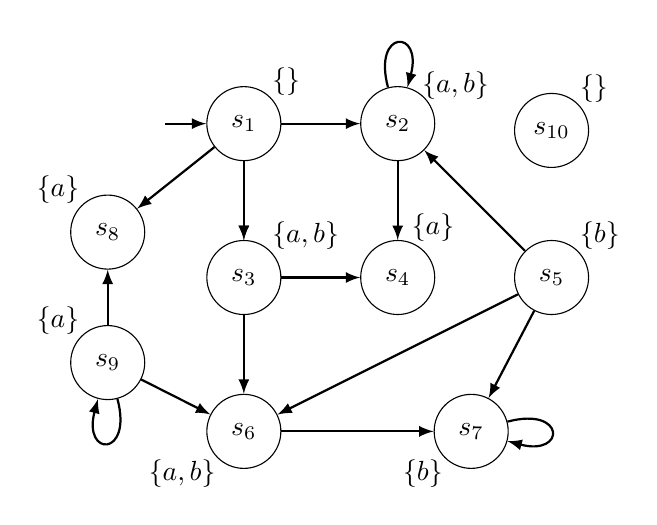
\begin{tikzpicture} [every initial by arrow/.style={thick}]
		%		\createstate{s1}{3,2+4}{$\state_1$};
		\path 
		(\basex,  \basey+2) node[mstate, initial, initial text=, initial distance=15pt] (s1) {$\state_1$} 
		;
		
		\node [mstate,right=of s1] (s2) {$\state_2$};
		\node [mstate,below=of s1] (s3) {$\state_3$};
		\node [mstate,below=of s2] (s4) {$\state_4$};
		\node [mstate,right=of s4] (s5) {$\state_5$};
%		\node [mstate,below right=40pt and 30 pt of s2] (s5) {$\state_5$};
		\node [mstate,below=of s3] (s6) {$\state_6$};
		\node [mstate,right=55pt of s6] (s7) {$\state_7$};
		\node [mstate,below left=20pt and 30pt of s1] (s8) {$\state_8$};
		\node [mstate,below=20pt of s8] (s9) {$\state_9$};
%		\node [mstate,right=of s2] (s10) {$\state_{10}$};
		\node [mstate,above=26pt of s5] (s10) {$\state_{10}$};
		
		\node [above right=-4pt of s1] (ls1) {$\{\}$};
		\node [above right=-6pt of s2] (ls2) {$\{a,b\}$};
		\node [above right=-4pt of s3] (ls3) {$\{a,b\}$};
		\node [above right=0pt and -8pt of s4] (ls4) {$\{a\}$};
		\node [above right=-4pt of s5] (ls5) {$\{b\}$};
		\node [below left=-4pt of s6] (ls6) {$\{a,b\}$};
		\node [below left=-4pt of s7] (ls7) {$\{b\}$};
		\node [above left=-4pt of s8] (ls8) {$\{a\}$};
		\node [above left=-4pt of s9] (ls9) {$\{a\}$};
		\node [above right=-4pt of s10] (ls10) {$\{\}$};
		

		
		
		\path [trans] (s1) edge (s2);
		\path [trans] (s1) edge (s3);
		\path [trans] (s1) edge (s3);
		\path [trans] (s1) edge (s8);
		\path [trans] (s2) edge (s4);
		\path [trans] (s3) edge (s4);
		\path [trans] (s3) edge (s6);
		\path [trans] (s5) edge (s2);
		\path [trans] (s5) edge (s6);
		\path [trans] (s5) edge (s7);
		\path [trans] (s6) edge (s7);
		\path [trans] (s9) edge (s8);
		\path [trans] (s9) edge (s6);
		
		\path [trans] (s2) edge [loop above] (s2);
		\path [trans] (s7) edge [loop right] (s7);
		\path [trans] (s9) edge [loop below] (s9);
		
	\end{tikzpicture}
\end{document}
	\end{minipage}%
	\begin{minipage}{.5\textwidth}
	\documentclass[tikz,preview]{standalone}
%\usepackage{prelude}

%%%%%%%%%%%%%%%%%%%%%%%%%%%%%%%%%%%% PACKAGES %%%%%%%%%%%%%%%%%%%%%%%%%%%%%%%%%%%%%%%%%%

\usepackage{inputenc,fontenc}
\usepackage[a4paper,margin=3cm]{geometry}
\usepackage[english]{babel}
%\usepackage[german]{babel}
%\usepackage[fixlanguage]{babelbib}


\usepackage{bbold}
\usepackage{amsthm}
\usepackage{amsmath}
\usepackage{amssymb} % doteqdot
\usepackage[dvipsnames]{xcolor}
\usepackage{standalone}
\usepackage{tikz}[mode=buildnew]
\usepackage{cite}
\usepackage{xspace}
\usepackage{relsize}
\usepackage{mathtools} % mathclap
%\usepackage{MnSymbol}
\usepackage{hyperref}
\usepackage{url}
\usepackage{listings} % for code
\usepackage[T1]{fontenc} %<
\hypersetup{
	colorlinks,
	citecolor=black,
	filecolor=black,
	linkcolor=black,
	urlcolor=black
}
\usepackage{pgfplots}
\pgfplotsset{compat=1.18}
%\usepackage{courier} %% Sets font for listing as Courier. But also for url and texttt!
\usepackage{listings, xcolor}
\usepackage{graphicx}
\usepackage{subcaption}

\usetikzlibrary{calc}
%\usepackage{xparse} % \newDocumentCommand for multiple optional arguments
%\usepackage{titlecaps}



%%%%%%%%%%%%%%%%%%%%%%%%%%%%%%%%%%%% THEOREMSTYLES %%%%%%%%%%%%%%%%%%%%%%%%%%%%%%%%%%

\theoremstyle{definition}
\newtheorem{definition}{Definition}[section]
\newtheorem{exmp}{Beispiel}[section]
%\AfterEndEnvironment{definition}{\noindent\ignorespaces}

\theoremstyle{theorem}
\newtheorem{theorem}{Satz}[section]
\newtheorem{proposition}{Proposition}[section]
%\AfterEndEnvironment{theorem}{\noindent\ignorespaces}

\theoremstyle{korollary}
\newtheorem{korollary}{Korollar}[section]
%\AfterEndEnvironment{korollary}{\noindent\ignorespaces}


\tikzset{
	mstate/.style={draw, circle, minimum size=.94cm}, 
	gstate/.style={draw, rectangle, minimum size=.8cm},
	varstate/.style={draw,rectangle, rounded corners, minimum size=1}, 
	trans/.style={draw, ->, thick},
	bendtrans/.style={draw, ->, thick, bend left=10},
	bendtransr/.style={draw, ->, thick, bend right=10},
	init/.style={initial, initial distance=6pt, initial text=},
	every loop/.style={min distance=5pt, looseness=8},
	>=latex
}
\usetikzlibrary{automata,positioning}

%auto shift/.style={auto=right,->,
%	to path={ let \p1=(\tikztostart),\p2=(\tikztotarget),
%		\n1={atan2(\y2-\y1,\x2-\x1)},\n2={\n1+180}
%		in ($(\tikztostart.{\n1})!1mm!270:(\tikztotarget.{\n2})$) -- 
%		($(\tikztotarget.{\n2})!1mm!90:(\tikztostart.{\n1})$) \tikztonodes}},

%%%%%%%%%%%%%%%%%%%%%%%%%%%%%%%%%%% MY MACROS %%%%%%%%%%%%%%%%%%%%%%%%%%%%%%%%%%%%%%%%%
%formatting
\newcommand{\comment}[2]{{\color{#1}#2}}
\newcommand{\redcomment}[1]{{\color{red}#1}}
\newcommand{\purpcomment}[1]{{\color{pink}#1}}
\newcommand{\bluecomment}[1]{{\color{blue}#1}}
\newcommand{\mt}[1]{\ensuremath{{#1}}\xspace}
\newcommand{\mynewcommand}[2]{\newcommand{#1}{\mt{#2}}} %% currently not used becaue of ide highlighting
\newcommand{\arr}{\mt{\to}}

%model checking terms
\newcommand{\mimicrel}{\mt{\mathcal{R}}}
\newcommand{\bisimeq}{\mt{\;\!\sim\;\!}}
\newcommand{\simorder}{\mt{\;\!\preceq\;\!}}
\newcommand{\simequiv}{\mt{\;\!\simeq\;\!}} %command already defined
\newcommand{\relts}{\mt{\;\!\bullet_{_{\tiny{TS}}}\;\!}}
\newcommand{\rel}{\mt{\;\!\bullet\;\!}}

%own names
\newcommand{\nm}[1]{#1\xspace}
\newcommand{\mdpN}{\nm{MDP}}
\newcommand{\mdpsN}{\nm{MDPs}}
\newcommand{\viewN}{\nm{view}}
\newcommand{\viewNC}{\nm{View}}
\newcommand{\viewsN}{\nm{views}}
\newcommand{\viewsNC}{\nm{Views}}
\newcommand{\grpfctsubN}{\nm{detached grouping function}}
\newcommand{\grpfctsubNC}{\nm{detached grouping function}}
\newcommand{\grpfctsubNCC}{\nm{Detached Grouping Function}}
\newcommand{\grpfctN}{\nm{grouping function}}
\newcommand{\grpfctNC}{\nm{Grouping function}}
\newcommand{\grpfctNCC}{\nm{Grouping Function}}
\newcommand{\grpfctsN}{\nm{grouping functions}}
\newcommand{\grpfctsNC}{\nm{Grouping functions}}
\newcommand{\grpfctsNCC}{\nm{Grouping Functions}}
\newcommand{\stmimicN}{\nm{state-mimic}}
\newcommand{\stmimicsN}{\nm{state-mimics}}
\newcommand{\stmimickingN}{\nm{state-mimicking}}
\newcommand{\stmimickedN}{\nm{state-mimicked}}
%\newcommand{\chosenphtypeNCC}{\nm{Transition System}}
%\newcommand{\chgphNC}{\nm{Transition system}}
%\newcommand{\chgphN}{\nm{transition system}}
%\newcommand{\chgphsNCC}{\nm{Transition Systems}}
%\newcommand{\chgphsNC}{\nm{Transition systems}}
%\newcommand{\chgphsN}{\nm{transition systems}}
\newcommand{\chgphNCC}{\nm{MDP}}
\newcommand{\chgphNC}{\nm{MDP}}
\newcommand{\chgphN}{\nm{MDP}}
\newcommand{\achgphN}{\nm{an MDP}}
\newcommand{\chgphsNCC}{\nm{MDPs}}
\newcommand{\chgphsNC}{\nm{MDPs}}
\newcommand{\chgphsN}{\nm{MDPs}}
\newcommand{\parllcompN}{\nm{parallel composition}}
\newcommand{\parllcompNC}{\nm{Parallel composition}}
\newcommand{\parllcompNCC}{\nm{Parallel Composition}}
\newcommand{\parllcompsN}{\nm{parallel compositions}}
\newcommand{\parllcompsNC}{\nm{Parallel compositions}}
\newcommand{\parllcompsNCC}{\nm{Parallel Compositions}}
\newcommand{\sccN}{\nm{SCC}}
\newcommand{\sccsN}{\nm{SCCs}}
\newcommand{\bsccN}{\nm{BSCC}}
\newcommand{\bsccsN}{\nm{BSCCs}}
\newcommand{\jgrapht}{\nm{jGraphtT}}

\newcommand{\outactident}{\nm{OutActionsIdent}}

%names
\newcommand{\iffN}{\nm{if and only if}}
\newcommand{\tsN}{\nm{TS}}

%% outactions identical
\newcommand{\outactidentstrong}{\nm{strong}}
\newcommand{\outactidentweak}{\nm{weak}}

% CORE DEFINITIONS
\newcommand{\grpfct}[1][\viewppty]{\mt{F_{#1}}}
\newcommand{\grpfctsub}[1][\viewppty]{\mt{\tilde{F}_{#1}}}
%\newcommand{\grpfctimg}[1]{\mt{{\grpfct}[{#1}]}}
%\newcommand{\fctimg}[2]{\mt{{#1}[{#2}]}}
\newcommand{\eqrelview}{\mt{R}}
\newcommand{\eqclassv}[1][\state]{\mt{\eqclass{#1}{\eqrelview}}}
\newcommand{\eqclasssetv}[1][\states]{\mt{{#1}/\eqrelview}} %OLD: \bigcup_{\state \in \states} \eqclassv
\newcommand{\viewid}{\mt{\mdp}}
\newcommand{\view}[1][\viewppty]{\mt{\viewid_{#1}}}
\newcommand{\imggrp}{\mt{\arbset}}
\newcommand{\imggrpsub}{\mt{X}}
\newcommand{\viewppty}{\mt{\theta}}
\newcommand{\pll}{\mt{\;\!\pllpure\;\!}}
\newcommand{\pllrev}{\mt{\pllpure^{-1}}}
\newcommand{\pllpure}{\mt{||}}
\newcommand{\compselectset}{\mt{Z}}
\newcommand{\compselectpure}{\mt{\pllpure_\compselectset}}
\newcommand{\compselect}{\mt{\;\pllpure_\compselectset\;}}
\newcommand{\remstates}{\mt{\bigcup_{\state \in \states \setminus \states_1}\{\{\state\}\}}}
\newcommand{\nogroupstates}[1][\states_2]{\mt{\bigcup_{\state \in \states \setminus {#1}}\{\{\state\}\}}}
\newcommand{\remelem}{\mt{\bullet}}
\newcommand{\nogroupset}{\mt{\xi}}
\newcommand{\remset}{\mt{\{\remelem\}}}
\newcommand{\gfctpll}{\mt{\grpfct[\pll]}}
\newcommand{\group}{\mt{\top}}
\newcommand{\imggrpbinview}{\mt{\{\remelem, \notppty\}}}
\newcommand{\viewappset}{\mt{\tilde{\states}}}
\newcommand{\hasppty}{\mt{\top}}
\newcommand{\notppty}{\mt{\bot}}
\newcommand{\disregardelem}{\mt{\Delta}}
\newcommand{\disregardelements}{\mt{{\disregardelem_1, \dots, \disregardelem_n}}}



%\newcommand{\mdp}{def}\mdp
%\newcommand{\mdpdef}



% EXAMPLE VIEWS
\newcommand{\pptyatomicprops}{\mt{\atomicprops}}
\newcommand{\pptyinitstates}{\mt{\initstates}}
\newcommand{\pptyinactsetsize}{\mt{|\inacts(\state)|}}
\newcommand{\pptyhasoutact}{\mt{\exists\outact}}
\newcommand{\pptyminoutact}[2]{\mt{#1\leq#2}}
\newcommand{\pptymaxoutact}[2]{\mt{#2\leq#1}}
\newcommand{\pptyspanoutact}[3]{\mt{#1\leq#2\leq#3}}
\newcommand{\pptyoutactsetsize}{\mt{|\outacts(\state)|}}
\newcommand{\pptyoutactsingle}{\mt{|\outacts(\state)|_1}}
\newcommand{\pptystrongoutactident}{\mt{\outacts(\state)_=}}
\newcommand{\pptyweakoutactident}{\mt{\outacts(\state)_\approx}}
\newcommand{\pptyhasinact}{\mt{\exists\inact}}
\newcommand{\pptymininact}[2]{\mt{#1\leq#2}}
\newcommand{\pptymaxinact}[2]{\mt{#2\leq#1}}
\newcommand{\pptyspaninact}[3]{\mt{#1\leq#2\leq#3}}
\newcommand{\pptyinactsingle}{\mt{|\inacts(\state)|_1}}
\newcommand{\pptystronginactident}{\mt{\inacts(\state)_=}}
\newcommand{\pptyweakinactident}{\mt{\inacts(\state)_\approx}}
\newcommand{\pptyparamvalueseq}{\mt{\var = \varval}}
\newcommand{\pptyparamvaluesneq}{\mt{\var \neq \varval}}
\newcommand{\pptyparamdnf}{\mt{VarDNF}}
\newcommand{\pptyparamcnf}{\mt{VarCNF}}
\newcommand{\pptyparamvalueseqopt}{\mt{\var = \varval}}
\newcommand{\pptyparamvalident}{\mt{Var:\varval}}
\newcommand{\pptydistance}{\mt{\distpath}}
\newcommand{\pptydistancerev}{\mt{\distpathrev}}
\newcommand{\pptydistancebi}{\mt{\distpathbi}}
\newcommand{\pptyhascycle}{\mt{\exists\cycle}}
\newcommand{\pptyexactactcycle}{\mt{\{\cycle_{\action,n}\}}}
\newcommand{\pptycycleset}{\mt{\cup{\{\state\}_\cycle}}}
\newcommand{\pptyexactcycle}{\mt{\{\cycle_n\}}}
\newcommand{\pptyscc}{\mt{scc}}
\newcommand{\pptybscc}{\mt{bscc}}
\newcommand{\pptyprop}{\mt{\redcomment{?}}}
\newcommand{\pptyident}{id}


\newcommand{\gfctatomicprops}{\mt{\grpfct[\pptyatomicprops]}}
\newcommand{\gfctinitstates}{\mt{\grpfct[\pptyinitstates]^\hasppty}}
\newcommand{\gfcthasoutaction}{\mt{\grpfct[\pptyhasoutact]^\hasppty}}
\newcommand{\gfctminoutaction}{\mt{\grpfct[\pptyminoutact{\numoutact}{\outact}]^\hasppty}}
\newcommand{\gfctmaxoutaction}{\mt{\grpfct[\pptymaxoutact{\numoutact}{\outact}]^\hasppty}}
\newcommand{\gfctspanoutaction}{\mt{\grpfct[\pptyspanoutact{\numoutactb}{\outact}{\numoutact}]^\hasppty}}
\newcommand{\gfctoutactsetsize}{\mt{\grpfct[\pptyoutactsetsize]}}
\newcommand{\gfctoutactsingle}{\mt{\grpfct[\pptyoutactsingle]^\notppty}}
\newcommand{\gfctstrongoutactident}{\mt{\grpfct[\pptystrongoutactident]}}
\newcommand{\gfctweakoutactident}{\mt{\grpfct[\pptyweakoutactident]}}
\newcommand{\gfcthasinaction}{\mt{\grpfct[\pptyhasinact]^\hasppty}}
\newcommand{\gfctmininaction}{\mt{\grpfct[\pptymininact{\numinact}{\inact}]^\hasppty}}
\newcommand{\gfctmaxinaction}{\mt{\grpfct[\pptymaxinact{\numinact}{\inact}]^\hasppty}}
\newcommand{\gfctspaninaction}{\mt{\grpfct[\pptyspaninact{\numinactb}{\inact}{\numinact}]^\hasppty}}
\newcommand{\gfctinactsetsize}{\mt{\grpfct[\pptyinactsetsize]}}
\newcommand{\gfctinactsingle}{\mt{\grpfct[\pptyinactsingle]^\notppty}}
\newcommand{\gfctstronginactident}{\mt{\grpfct[\pptystronginactident]}}
\newcommand{\gfctweakinactident}{\mt{\grpfct[\pptyweakinactident]}}
\newcommand{\gfctparamvalueseq}{\mt{\grpfct[\pptyparamvalueseq]^\hasppty}}
\newcommand{\gfctparamvaluesneq}{\mt{\grpfct[\pptyparamvaluesneq]^\hasppty}}
\newcommand{\gfctparamdnf}{\mt{\grpfct[\pptyparamdnf]^\hasppty}}
\newcommand{\gfctparamcnf}{\mt{\grpfct[\pptyparamcnf]^\hasppty}}
\newcommand{\gfctparamvalueseqopt}{\mt{\pptyparamvalueseqopt}}
\newcommand{\gfctparamvalident}{\mt{\grpfct[\pptyparamvalident]}}
\newcommand{\gfctdistance}{\mt{\grpfct[\pptydistance]}}
\newcommand{\gfctdistancerev}{\mt{\grpfct[\pptydistancerev]}}
\newcommand{\gfctdistancebi}{\mt{\grpfct[\pptydistancebi]}}
\newcommand{\gfcthascycle}{\mt{\grpfct[\pptyhascycle]}}
\newcommand{\gfctexactcycle}{\mt{\grpfct[\pptyexactcycle]}}
\newcommand{\gfctcycleset}{\mt{\grpfct[\pptycycleset]}}
\newcommand{\gfctexactactcycle}{\mt{\grpfct[\pptyexactactcycle]}}
\newcommand{\gfctscc}{\mt{\grpfct[\pptyscc]}}
\newcommand{\gfctbscc}{\mt{\grpfct[\pptybscc]}}
\newcommand{\gfctprop}{\mt{\grpfct[\pptyprop]}}
\newcommand{\gfctident}{\mt{\grpfct[\pptyident]}}

\newcommand{\gfctsubatomicprops}{\mt{\grpfctsub[\pptyatomicprops]}}
\newcommand{\gfctsubinitstates}{\mt{\grpfctsub[\pptyinitstates]^\hasppty}}
\newcommand{\gfctsubhasoutaction}{\mt{\grpfctsub[\pptyhasoutact]^\hasppty}}
\newcommand{\gfctsubminoutaction}{\mt{\grpfctsub[\pptyminoutact{\numoutact}{\outact}]^\hasppty}}
\newcommand{\gfctsubmaxoutaction}{\mt{\grpfctsub[\pptymaxoutact{\numoutact}{\outact}]^\hasppty}}
\newcommand{\gfctsubspanoutaction}{\mt{\grpfctsub[\pptyspanoutact{\numoutactb}{\outact}{\numoutact}]^\hasppty}}
\newcommand{\gfctsuboutactsetsize}{\mt{\grpfctsub[\pptyoutactsetsize]}}
\newcommand{\gfctsuboutactsingle}{\mt{\grpfctsub[\pptyoutactsingle]^\notppty}}
\newcommand{\gfctsubstrongoutactident}{\mt{\grpfctsub[\pptystrongoutactident]^\hasppty}}
\newcommand{\gfctsubweakoutactident}{\mt{\grpfctsub[\pptyweakoutactident]^\hasppty}}
\newcommand{\gfctsubhasinaction}{\mt{\grpfctsub[\pptyhasinact]}}
\newcommand{\gfctsubmininaction}{\mt{\grpfctsub[\pptymininact{\numinact}{\inact}]}}
\newcommand{\gfctsubmaxinaction}{\mt{\grpfctsub[\pptymaxinact{\numinact}{\inact}]}}
\newcommand{\gfctsubspaninaction}{\mt{\grpfctsub[\pptyspaninact{\numinactb}{\inact}{\numinact}]}}
\newcommand{\gfctsubinactsetsize}{\mt{\grpfctsub[\pptyinactsetsize]^\hasppty}}
\newcommand{\gfctsubinactsingle}{\mt{\grpfctsub[\pptyinactsingle]^\notppty}}
\newcommand{\gfctsubstronginactident}{\mt{\grpfctsub[\pptystronginactident]}}
\newcommand{\gfctsubweakinactident}{\mt{\grpfctsub[\pptyweakinactident]}}
\newcommand{\gfctsubparamvalueseq}{\mt{\grpfctsub[\pptyparamvalueseq]^\hasppty}}
\newcommand{\gfctsubparamvaluesneq}{\mt{\grpfctsub[\pptyparamvaluesneq]^\hasppty}}
\newcommand{\gfctsubparamdnf}{\mt{\grpfctsub[\pptyparamdnf]^\hasppty}}
\newcommand{\gfctsubparamcnf}{\mt{\grpfctsub[\pptyparamcnf]^\hasppty}}
\newcommand{\gfctsubparamvalueseqopt}{\mt{\pptyparamvalueseqopt}}
\newcommand{\gfctsubparamvalident}{\mt{\grpfctsub[\pptyparamvalident]}}
\newcommand{\gfctsubdistance}{\mt{\grpfctsub[\pptydistance]}}
\newcommand{\gfctsubdistancerev}{\mt{\grpfctsub[\pptydistancerev]}}
\newcommand{\gfctsubdistancebi}{\mt{\grpfctsub[\pptydistancebi]}}
\newcommand{\gfctsubhascycle}{\mt{\grpfctsub[\pptyhascycle]^\hasppty}}
\newcommand{\gfctsubexactcycle}{\mt{\grpfctsub[\pptyexactcycle]}}
\newcommand{\gfctsubcycleset}{\mt{\grpfctsub[\pptycycleset]}}
\newcommand{\gfctsubexactactcycle}{\mt{\grpfctsub[\pptyexactactcycle]}}
\newcommand{\gfctsubscc}{\mt{\grpfctsub[\pptyscc]}}
\newcommand{\gfctsubbscc}{\mt{\grpfctsub[\pptybscc]}}
\newcommand{\gfctsubprop}{\mt{\grpfctsub[\pptyprop]}}
\newcommand{\gfctsubident}{\mt{\grpfctsub[\pptyident]}}


\newcommand{\viewatomicprops}{\mt{\view[\pptyatomicprops]}}
\newcommand{\viewinitstates}{\mt{\view[\pptyinitstates]^\hasppty}}
\newcommand{\viewhasoutaction}{\mt{\view[\pptyhasoutact]^\hasppty}}
\newcommand{\viewminoutaction}{\mt{\view[\pptyminoutact{\numoutact}{\outact}]^\hasppty}}
\newcommand{\viewmaxoutaction}{\mt{\view[\pptymaxoutact{\numoutact}{\outact}]^\hasppty}}
\newcommand{\viewspanoutaction}{\mt{\view[\pptyspanoutact{\numoutactb}{\outact}{\numoutact}]^\hasppty}}
\newcommand{\viewoutactsetsize}{\mt{\view[\pptyoutactsetsize]}}
\newcommand{\viewoutactsingle}{\mt{\view[\pptyoutactsingle]^\notppty}}
\newcommand{\viewstrongoutactident}{\mt{\view[\pptystrongoutactident]}}
\newcommand{\viewweakoutactident}{\mt{\view[\pptyweakoutactident]}}
\newcommand{\viewhasinaction}{\mt{\view[\pptyhasinact]^\hasppty}}
\newcommand{\viewmininaction}{\mt{\view[\pptymininact{\numinact}{\inact}]^\hasppty}}
\newcommand{\viewmaxinaction}{\mt{\view[\pptymaxinact{\numinact}{\inact}]^\hasppty}}
\newcommand{\viewspaninaction}{\mt{\view[\pptyspaninact{\numinactb}{\inact}{\numinact}]^\hasppty}}
\newcommand{\viewinactsetsize}{\mt{\view[\pptyinactsetsize]}}
\newcommand{\viewinactsingle}{\mt{\view[\pptyinactsingle]^\notppty}}
\newcommand{\viewstronginactident}{\mt{\view[\pptystronginactident]}}
\newcommand{\viewweakinactident}{\mt{\view[\pptyweakinactident]}}
\newcommand{\viewparamvalueseq}{\mt{\view[\pptyparamvalueseq]}}
\newcommand{\viewparamvaluesneq}{\mt{\view[\pptyparamvaluesneq]}}
\newcommand{\viewparamdnf}{\mt{\view[\pptyparamdnf]^\hasppty}}
\newcommand{\viewparamcnf}{\mt{\view[\pptyparamcnf]^\hasppty}}
\newcommand{\viewparamvalueseqopt}{\mt{\pptyparamvalueseqopt}}
\newcommand{\viewparamvalident}{\mt{\view[\pptyparamvalident]}}
\newcommand{\viewdistance}{\mt{\view[\pptydistance]}}
\newcommand{\viewdistancerev}{\mt{\view[\pptydistancerev]}}
\newcommand{\viewdistancebi}{\mt{\view[\pptydistancebi]}}
\newcommand{\viewhascycle}{\mt{\view[\pptyhascycle]}}
\newcommand{\viewexactcycle}{\mt{\view[\pptyexactcycle]}}
\newcommand{\viewcycleset}{\mt{\view[\pptycycleset]}}
\newcommand{\viewexactactcycle}{\mt{\view[\pptyexactactcycle]}}
\newcommand{\viewscc}{\mt{\view[\pptyscc]}}
\newcommand{\viewbscc}{\mt{\view[\pptybscc]}}
\newcommand{\viewprop}{\mt{\view[\pptyprop]}}
\newcommand{\viewident}{\mt{\view[\pptyident]}}

%\newcommand{\viewatomicprops}{\mt{\view[\atomicprops]}}
%\newcommand{\viewinitstates}{\mt{\view[\initstates]}}
%\newcommand{\viewhasoutaction}{\mt{\view[\pptyhasoutact]}}
%\newcommand{\viewminoutaction}{\mt{\view[\pptyminoutact{\numoutact}{\outact}]}}
%\newcommand{\viewmaxoutaction}{\mt{\view[\pptymaxoutact{\numoutact}{\outact}]}}
%\newcommand{\viewspanoutaction}{\mt{\view[\pptyspanoutact{\numoutactb}{\outact}{\numoutact}]}}
%\newcommand{\viewoutactsetsize}{\mt{\view[\pptyoutactsetsize]}}
%\newcommand{\viewoutactsingle}{\mt{\view[\pptyoutactsingle]}}
%\newcommand{\viewstrongoutactident}{\mt{\view[\outacts(\state)_=]}}
%\newcommand{\viewweakoutactident}{\mt{\view[\outacts(\state)_\approx]}}
%\newcommand{\viewhasinaction}{\mt{\view[\pptyhasinact]}}
%\newcommand{\viewmininaction}{\mt{\view[\pptymininact{\numinact}{\inact}]}}
%\newcommand{\viewmaxinaction}{\mt{\view[\pptymaxinact{\numinact}{\inact}]}}
%\newcommand{\viewspaninaction}{\mt{\view[\pptyspaninact{\numinactb}{\inact}{\numinact}]}}
%\newcommand{\viewinactsetsize}{\mt{\view[\pptyinactsetsize]}}
%\newcommand{\viewinactsingle}{\mt{\view[\pptyinactsingle]}}
%\newcommand{\viewstronginactident}{\mt{\view[\inacts(\state)_=]}}
%\newcommand{\viewweakinactident}{\mt{\view[\inacts(\state)_\approx]}}
%\newcommand{\viewparamvalueseq}{\mt{\view[\var = \varval]}}
%\newcommand{\viewparamvaluesneq}{\mt{\view[\var \neq \varval]}}
%\newcommand{\viewparamdnf}{\mt{\view[VarDNF]}}
%\newcommand{\viewparamcnf}{\mt{\view[VarCNF]}}
%\newcommand{\viewparamvalident}{\mt{\view[\pptyparamvalident]}}
%\newcommand{\viewdistance}{\mt{\view[\pptydistance]}}
%\newcommand{\viewhascycle}{\mt{\view[\exists\cycle]}}
%\newcommand{\viewexactcycle}{\mt{\view[\pptyexactcycle]}}
%\newcommand{\viewcycleset}{\mt{\view[\pptycycleset]}}
%\newcommand{\viewexactactcycle}{\mt{\view[\pptyexactactcycle]}}
%\newcommand{\viewscc}{\mt{\view[scc]}}
%\newcommand{\viewbscc}{\mt{\view[bscc]}}

%actions
\newcommand{\numoutact}{\mt{n}}
\newcommand{\numoutactb}{\mt{m}}
\newcommand{\numinact}{\mt{n}}
\newcommand{\numinactb}{\mt{m}}

\newcommand{\predmaxoutact}[1][\numoutact]{\mt{Q_{\outact\leq#1}(\state,\state_1, \dots, \state_{#1+1})}}
\newcommand{\predminoutact}[1][\numoutact]{\mt{Q_{#1\leq\outact}(\state,\state_1, \dots, \state_{#1})}}
\newcommand{\formoutact}[1][\state]{\mt{C_{#1,\outact}}}
\newcommand{\predmaxinact}[1][\numinact]{\mt{Q_{\inact\leq#1}(\state,\state_1, \dots, \state_{#1+1})}}
\newcommand{\predmininact}[1][\numinact]{\mt{Q_{#1\leq\inact}(\state,\state_1, \dots, \state_{#1})}}

\newcommand{\outact}[1][\action]{\mt{\overrightarrow{#1}}}
\newcommand{\outacts}{\mt{\overrightarrow{\actions}}}
\newcommand{\inact}{\mt{\overleftarrow{\action}}}
\newcommand{\inacts}[1][\action]{\mt{\overleftarrow{#1}}}

%%Parameters
\newcommand{\vars}[1][\mdp]{\mt{V\!ar_{#1}}}
\newcommand{\var}{\mt{x}}
\newcommand{\varstate}[1][]{\mt{\var_{\state#1}}}
\newcommand{\varval}{\mt{a}}
\newcommand{\vareval}[1][\mdp]{\mt{V\!arEval_{#1}}}
\newcommand{\varevalimg}[1][\mdp]{\mt{\vareval[#1][\states,\vars]}}
\newcommand{\varevalimgset}{\mt{\arbset}}
\newcommand{\someparam}{\mt{\tilde{x}}}
\newcommand{\eqorneq}{\mt{\;\doteqdot\;}}
\newcommand{\varstyle}[2]{\mt{\langle#1,#2\rangle}}




%\makeatletter
%\newcommand{\overleftrightsmallarrow}{\mathpalette{\overarrowsmall@\leftrightarrowfill@}}
%\newcommand{\overrightsmallarrow}{\mathpalette{\overarrowsmall@\rightarrowfill@}}
%\newcommand{\overleftsmallarrow}{\mathpalette{\overarrowsmall@\leftarrowfill@}}
%\newcommand{\overarrowsmall@}[3]{%
%	\vbox{%
%		\ialign{%
%			##\crcr
%			#1{\smaller@style{#2}}\crcr
%			\noalign{\nointerlineskip}%
%			$\m@th\hfil#2#3\hfil$\crcr
%		}%
%	}%
%}
%\def\smaller@style#1{%
%	\ifx#1\displaystyle\scriptstyle\else
%	\ifx#1\textstyle\scriptstyle\else
%	\scriptscriptstyle
%	\fi
%	\fi
%}
%\makeatother
%\newcommand{\te}[1]{\overleftrightsmallarrow{#1}}

% Distance
\newcommand{\fctdist}{\mt{distance}}
\newcommand{\fctdistdefault}{\mt{\fctdist(\chgph, \smstates, \grandist)}}
\newcommand{\distval}{\mt{d}}
\newcommand{\grandist}{\mt{n}}
\let\path\oldpath
\newcommand{\path}{\mt{P}}
\newcommand{\pathbi}{\mt{\bar{\path}}}
\newcommand{\pathsecfull}{\mt{(\state_0, \action_0, \state_1, \action_1, \dots, \action_{n}, \state_{n+1})}}
\newcommand{\lenpath}{\mt{len}}
\newcommand{\pfirst}{\mt{first}}
\newcommand{\plast}{\mt{last}}
\newcommand{\pathset}{\mt{\path_\chgph}}
\newcommand{\pathbiset}{\mt{\pathbi_\chgph}}
\newcommand{\distpath}{\mt{\overrightarrow{dist}}}
\newcommand{\distpathrev}{\mt{\overleftarrow{dist}}}
\newcommand{\distpathbi}{\mt{\overline{dist}}}
%Cycles
\newcommand{\cyclesecfull}{\mt{(\state_0, \action_0, \state_1, \action_1, \dots, \action_{n-1}, \state_0)}}
\newcommand{\fctfindcycles}{\mt{findCycles}}
\newcommand{\cycle}{\mt{C}}
\newcommand{\cycleset}{\mt{\cycle_{\mdp, n}}}
\newcommand{\lencycle}{\mt{len}}
% strongly connected components
\newcommand{\scc}{\mt{T}}
\newcommand{\setscc}{\mt{SCC_{\chgph,n}}}
\newcommand{\setbscc}{\mt{BSCC_{\chgph,n}}}

% properties
\newcommand{\propfct}{\mt{f}}

% all Systems
\newcommand{\chgph}{\mt{\mdp}}
\newcommand{\chgphtuple}{\mt{\mdptuple}}
\newcommand{\chgphtupledist}{\mt{\mdptupledist}}

\newcommand{\states}{\mt{S}}
\newcommand{\actions}{\mt{Act}}
\newcommand{\atomicprops}{\mt{AP}}
\newcommand{\labelingfct}{\mt{L}}
\newcommand{\init}{\mt{\initdistrib}} % use MDP % refers to the underlying set
\newcommand{\trans}{\mt{\probtfunc}} % use MDP % refers to the underlying set
\newcommand{\smstates}{\mt{\tilde{\states}}}


\newcommand{\state}{\mt{s}}
\newcommand{\action}{\mt{\alpha}}
\newcommand{\actionb}{\mt{\beta}}
\newcommand{\actionc}{\mt{\gamma}}
\newcommand{\smstate}{\mt{\tilde{\state}}}



% transition sysstems
\newcommand{\ts}{\mt{TS}}
\newcommand{\transitionrel}{\mt{\longrightarrow}}
\newcommand{\initstates}{\mt{I}}
\newcommand{\transitionsystem}{\mt
	{(\states, \actions, \transitionrel, \initstates, \atomicprops, \labelingfct)}
}
\newcommand{\tstupledist}{\mt{(\states', \actions',\transitionrel', \initstates', \labelingfct')}}


%Markov chains and MDP
\newcommand{\mdp}{\mt{\autm}}
\newcommand{\mdptuple}{\mt{(\states, \actions, \probtfunc, \initdistrib, \atomicprops, \labelingfct)}}
\newcommand{\mdptupledist}{\mt{(\states', \actions', \probtfunc', \initdistrib', \atomicprops', \labelingfct')}}
\newcommand{\autm}{\mt{\mathcal{M}}}
\newcommand{\probtfunc}{\mt{\textbf{P}}}
\newcommand{\initdistrib}{\mt{\iota_{init}}}


%maths
\newcommand{\powerset}[1]{\mt{\mathcal{P}(#1)}}
\newcommand{\eqclass}[2]{\mt{[#1]_{#2}}}%{\mt{#1 / #2}}
\newcommand{\impr}{\mt{\hspace{3mm}\Rightarrow\hspace{2mm}}}
\newcommand{\impl}{\mt{\hspace{3mm}\Leftarrow\hspace{2mm}}}
\newcommand{\natnums}{\mt{\mathbb{N}}} 
\newcommand{\realnums}{\mt{\mathbb{R}}}
\newcommand{\intmodn}[1][n]{\mt{\mathbb{Z}_{#1}}}
\newcommand{\arbset}{\mt{M}}
\newcommand{\bigsum}[2][]{\mt{\mathlarger{\sum}_{#2}^{#1}}}
\newcommand{\bbigsum}[2][]{\mt{\mathlarger{\mathlarger{\sum}}_{#2}^{#1}}}
\newcommand{\invimage}[2]{#1^{\mt{-1}(#2)}}
\newcommand{\img}{\mt{Img}}
\newcommand{\cond}{\mt{\,|\,}}

%tickz
%% \definecolor{darkred}{RGB}{196, 42, 42}

%implementation
\newcommand{\pmcvis}{\nm{PMC-Vis}}





\begin{document}
	\newcommand{\basex}{0}
	\newcommand{\basey}{-.4}
	\newcommand{\createstate}[3]{\node[draw, circle, minimum size=1cm] (#1) at (#2) {#3}}
	
	
	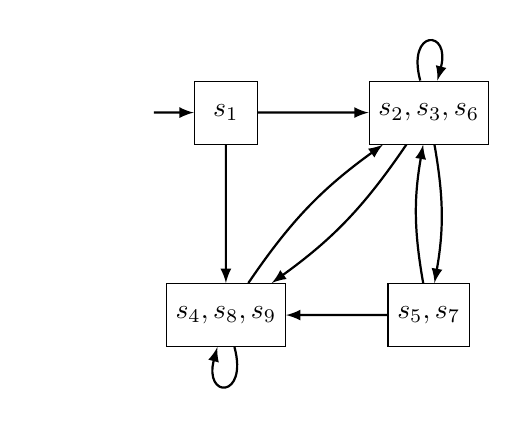
\begin{tikzpicture} [scale=2.4, every initial by arrow/.style={thick}]
		
		\newcommand{\disth}{40pt}
		\newcommand{\distv}{50pt}
		
		\node at (0,0) {};
		
		\node [gstate,init] (s1) at (\basex,\basey) {$\state_1$};
		\node [gstate,right=\disth of s1] (s236) {$\state_2,\state_3,\state_6$};
		\node [gstate,below=\distv of s1] (s489) {$\state_4,\state_8,\state_9$};
		\node [gstate,below=\distv of s236] (s57) {$\state_5,\state_7$};
		
		\path [trans] (s1) edge (s236);
		\path [trans] (s1) edge (s489);
		\path [trans] (s57) edge (s489);
		\path [bendtrans] (s57) edge (s236);
		\path [bendtrans] (s236) edge (s57);
		\path [bendtrans] (s236) edge (s489);
		\path [bendtrans] (s489) edge (s236);
		
		\path [trans] (s236) edge [loop above] (s236);
		\path [trans] (s489) edge [loop below] (s489);
			
		
		%		midway, at start, near start, very near start, at end, near end, very near end
		
		
	\end{tikzpicture}
\end{document}
	\end{minipage}
	\caption{Simplified representations of \mdp (left) and the \viewN \viewatomicprops on it (right)}
	\label{fig:apIdentBeforeAfter}  
\end{figure}


\subsubsection{Initial States}
An a little more involved idea than directly using a given function is to utilize the set of initial states. We can group states that have a probability greater zero, that they are started from. In practice this might be useful to quickly find all initial states.

\begin{definition}
	Let $\chgph = \chgphtuple$ be \achgphN and $\initstates := \{\state \in \states \mid \state \in \init\}$. The view \viewinitstates is defined by its \grpfctN with $\gfctinitstates : \states \to \imggrp$ with 
	
	\[
	\state \mapsto
	\begin{cases}
			\group,				& \text{if } \state \in \initstates \\
			\remelem,          	& \text{otherwise}
		\end{cases}
	\]
	
	and $\imggrp := \imggrpbinview$.
\end{definition}

For $\state_1,\state_2 \in \states$ it is $\gfctinitstates(\state_1) = \gfctinitstates(\state_2)$ \iffN $\state_1, \state_2 \in \initstates$ or $\state_1 = \state_2$. According to Definition \ref{def:eqrelview} it is 
\begin{align*}
	\eqclassv &= \{\state \in \states \mid \gfctinitstates(\state) = \group\} &\text{for } \state \in \initstates \text{ and} \\
	\eqclassv &= \{\state \in \states \mid \gfctinitstates(\state) = \{\state\} \} = \{\state\} &\text{for } \state \notin \initstates.
\end{align*}


By this we obtain the \viewN $\viewinitstates$ for a given \achgphN \chgph where: $\states' = \bigcup_{\state \in \states} \{\eqclassv\} = \{\state \in \states \mid \state \in \initstates\}\cup \bigcup_{\state \in \states \setminus \initstates}\{\{\state\}\}$.

All other components are constructed as in Definition \ref{def:view}.

\begin{figure}[h]
	\begin{minipage}{.5\textwidth}
		\hspace{5mm}
		\documentclass[tikz]{standalone}
%\usepackage{prelude}

%%%%%%%%%%%%%%%%%%%%%%%%%%%%%%%%%%%% PACKAGES %%%%%%%%%%%%%%%%%%%%%%%%%%%%%%%%%%%%%%%%%%

\usepackage{inputenc,fontenc}
\usepackage[a4paper,margin=3cm]{geometry}
\usepackage[english]{babel}
%\usepackage[german]{babel}
%\usepackage[fixlanguage]{babelbib}


\usepackage{bbold}
\usepackage{amsthm}
\usepackage{amsmath}
\usepackage{amssymb} % doteqdot
\usepackage[dvipsnames]{xcolor}
\usepackage{standalone}
\usepackage{tikz}[mode=buildnew]
\usepackage{cite}
\usepackage{xspace}
\usepackage{relsize}
\usepackage{mathtools} % mathclap
%\usepackage{MnSymbol}
\usepackage{hyperref}
\usepackage{url}
\usepackage{listings} % for code
\usepackage[T1]{fontenc} %<
\hypersetup{
	colorlinks,
	citecolor=black,
	filecolor=black,
	linkcolor=black,
	urlcolor=black
}
\usepackage{pgfplots}
\pgfplotsset{compat=1.18}
%\usepackage{courier} %% Sets font for listing as Courier. But also for url and texttt!
\usepackage{listings, xcolor}
\usepackage{graphicx}
\usepackage{subcaption}

\usetikzlibrary{calc}
%\usepackage{xparse} % \newDocumentCommand for multiple optional arguments
%\usepackage{titlecaps}



%%%%%%%%%%%%%%%%%%%%%%%%%%%%%%%%%%%% THEOREMSTYLES %%%%%%%%%%%%%%%%%%%%%%%%%%%%%%%%%%

\theoremstyle{definition}
\newtheorem{definition}{Definition}[section]
\newtheorem{exmp}{Beispiel}[section]
%\AfterEndEnvironment{definition}{\noindent\ignorespaces}

\theoremstyle{theorem}
\newtheorem{theorem}{Satz}[section]
\newtheorem{proposition}{Proposition}[section]
%\AfterEndEnvironment{theorem}{\noindent\ignorespaces}

\theoremstyle{korollary}
\newtheorem{korollary}{Korollar}[section]
%\AfterEndEnvironment{korollary}{\noindent\ignorespaces}


\tikzset{
	mstate/.style={draw, circle, minimum size=.94cm}, 
	gstate/.style={draw, rectangle, minimum size=.8cm},
	varstate/.style={draw,rectangle, rounded corners, minimum size=1}, 
	trans/.style={draw, ->, thick},
	bendtrans/.style={draw, ->, thick, bend left=10},
	bendtransr/.style={draw, ->, thick, bend right=10},
	init/.style={initial, initial distance=6pt, initial text=},
	every loop/.style={min distance=5pt, looseness=8},
	>=latex
}
\usetikzlibrary{automata,positioning}

%auto shift/.style={auto=right,->,
%	to path={ let \p1=(\tikztostart),\p2=(\tikztotarget),
%		\n1={atan2(\y2-\y1,\x2-\x1)},\n2={\n1+180}
%		in ($(\tikztostart.{\n1})!1mm!270:(\tikztotarget.{\n2})$) -- 
%		($(\tikztotarget.{\n2})!1mm!90:(\tikztostart.{\n1})$) \tikztonodes}},

%%%%%%%%%%%%%%%%%%%%%%%%%%%%%%%%%%% MY MACROS %%%%%%%%%%%%%%%%%%%%%%%%%%%%%%%%%%%%%%%%%
%formatting
\newcommand{\comment}[2]{{\color{#1}#2}}
\newcommand{\redcomment}[1]{{\color{red}#1}}
\newcommand{\purpcomment}[1]{{\color{pink}#1}}
\newcommand{\bluecomment}[1]{{\color{blue}#1}}
\newcommand{\mt}[1]{\ensuremath{{#1}}\xspace}
\newcommand{\mynewcommand}[2]{\newcommand{#1}{\mt{#2}}} %% currently not used becaue of ide highlighting
\newcommand{\arr}{\mt{\to}}

%model checking terms
\newcommand{\mimicrel}{\mt{\mathcal{R}}}
\newcommand{\bisimeq}{\mt{\;\!\sim\;\!}}
\newcommand{\simorder}{\mt{\;\!\preceq\;\!}}
\newcommand{\simequiv}{\mt{\;\!\simeq\;\!}} %command already defined
\newcommand{\relts}{\mt{\;\!\bullet_{_{\tiny{TS}}}\;\!}}
\newcommand{\rel}{\mt{\;\!\bullet\;\!}}

%own names
\newcommand{\nm}[1]{#1\xspace}
\newcommand{\mdpN}{\nm{MDP}}
\newcommand{\mdpsN}{\nm{MDPs}}
\newcommand{\viewN}{\nm{view}}
\newcommand{\viewNC}{\nm{View}}
\newcommand{\viewsN}{\nm{views}}
\newcommand{\viewsNC}{\nm{Views}}
\newcommand{\grpfctsubN}{\nm{detached grouping function}}
\newcommand{\grpfctsubNC}{\nm{detached grouping function}}
\newcommand{\grpfctsubNCC}{\nm{Detached Grouping Function}}
\newcommand{\grpfctN}{\nm{grouping function}}
\newcommand{\grpfctNC}{\nm{Grouping function}}
\newcommand{\grpfctNCC}{\nm{Grouping Function}}
\newcommand{\grpfctsN}{\nm{grouping functions}}
\newcommand{\grpfctsNC}{\nm{Grouping functions}}
\newcommand{\grpfctsNCC}{\nm{Grouping Functions}}
\newcommand{\stmimicN}{\nm{state-mimic}}
\newcommand{\stmimicsN}{\nm{state-mimics}}
\newcommand{\stmimickingN}{\nm{state-mimicking}}
\newcommand{\stmimickedN}{\nm{state-mimicked}}
%\newcommand{\chosenphtypeNCC}{\nm{Transition System}}
%\newcommand{\chgphNC}{\nm{Transition system}}
%\newcommand{\chgphN}{\nm{transition system}}
%\newcommand{\chgphsNCC}{\nm{Transition Systems}}
%\newcommand{\chgphsNC}{\nm{Transition systems}}
%\newcommand{\chgphsN}{\nm{transition systems}}
\newcommand{\chgphNCC}{\nm{MDP}}
\newcommand{\chgphNC}{\nm{MDP}}
\newcommand{\chgphN}{\nm{MDP}}
\newcommand{\achgphN}{\nm{an MDP}}
\newcommand{\chgphsNCC}{\nm{MDPs}}
\newcommand{\chgphsNC}{\nm{MDPs}}
\newcommand{\chgphsN}{\nm{MDPs}}
\newcommand{\parllcompN}{\nm{parallel composition}}
\newcommand{\parllcompNC}{\nm{Parallel composition}}
\newcommand{\parllcompNCC}{\nm{Parallel Composition}}
\newcommand{\parllcompsN}{\nm{parallel compositions}}
\newcommand{\parllcompsNC}{\nm{Parallel compositions}}
\newcommand{\parllcompsNCC}{\nm{Parallel Compositions}}
\newcommand{\sccN}{\nm{SCC}}
\newcommand{\sccsN}{\nm{SCCs}}
\newcommand{\bsccN}{\nm{BSCC}}
\newcommand{\bsccsN}{\nm{BSCCs}}
\newcommand{\jgrapht}{\nm{jGraphtT}}

\newcommand{\outactident}{\nm{OutActionsIdent}}

%names
\newcommand{\iffN}{\nm{if and only if}}
\newcommand{\tsN}{\nm{TS}}

%% outactions identical
\newcommand{\outactidentstrong}{\nm{strong}}
\newcommand{\outactidentweak}{\nm{weak}}

% CORE DEFINITIONS
\newcommand{\grpfct}[1][\viewppty]{\mt{F_{#1}}}
\newcommand{\grpfctsub}[1][\viewppty]{\mt{\tilde{F}_{#1}}}
%\newcommand{\grpfctimg}[1]{\mt{{\grpfct}[{#1}]}}
%\newcommand{\fctimg}[2]{\mt{{#1}[{#2}]}}
\newcommand{\eqrelview}{\mt{R}}
\newcommand{\eqclassv}[1][\state]{\mt{\eqclass{#1}{\eqrelview}}}
\newcommand{\eqclasssetv}[1][\states]{\mt{{#1}/\eqrelview}} %OLD: \bigcup_{\state \in \states} \eqclassv
\newcommand{\viewid}{\mt{\mdp}}
\newcommand{\view}[1][\viewppty]{\mt{\viewid_{#1}}}
\newcommand{\imggrp}{\mt{\arbset}}
\newcommand{\imggrpsub}{\mt{X}}
\newcommand{\viewppty}{\mt{\theta}}
\newcommand{\pll}{\mt{\;\!\pllpure\;\!}}
\newcommand{\pllrev}{\mt{\pllpure^{-1}}}
\newcommand{\pllpure}{\mt{||}}
\newcommand{\compselectset}{\mt{Z}}
\newcommand{\compselectpure}{\mt{\pllpure_\compselectset}}
\newcommand{\compselect}{\mt{\;\pllpure_\compselectset\;}}
\newcommand{\remstates}{\mt{\bigcup_{\state \in \states \setminus \states_1}\{\{\state\}\}}}
\newcommand{\nogroupstates}[1][\states_2]{\mt{\bigcup_{\state \in \states \setminus {#1}}\{\{\state\}\}}}
\newcommand{\remelem}{\mt{\bullet}}
\newcommand{\nogroupset}{\mt{\xi}}
\newcommand{\remset}{\mt{\{\remelem\}}}
\newcommand{\gfctpll}{\mt{\grpfct[\pll]}}
\newcommand{\group}{\mt{\top}}
\newcommand{\imggrpbinview}{\mt{\{\remelem, \notppty\}}}
\newcommand{\viewappset}{\mt{\tilde{\states}}}
\newcommand{\hasppty}{\mt{\top}}
\newcommand{\notppty}{\mt{\bot}}
\newcommand{\disregardelem}{\mt{\Delta}}
\newcommand{\disregardelements}{\mt{{\disregardelem_1, \dots, \disregardelem_n}}}



%\newcommand{\mdp}{def}\mdp
%\newcommand{\mdpdef}



% EXAMPLE VIEWS
\newcommand{\pptyatomicprops}{\mt{\atomicprops}}
\newcommand{\pptyinitstates}{\mt{\initstates}}
\newcommand{\pptyinactsetsize}{\mt{|\inacts(\state)|}}
\newcommand{\pptyhasoutact}{\mt{\exists\outact}}
\newcommand{\pptyminoutact}[2]{\mt{#1\leq#2}}
\newcommand{\pptymaxoutact}[2]{\mt{#2\leq#1}}
\newcommand{\pptyspanoutact}[3]{\mt{#1\leq#2\leq#3}}
\newcommand{\pptyoutactsetsize}{\mt{|\outacts(\state)|}}
\newcommand{\pptyoutactsingle}{\mt{|\outacts(\state)|_1}}
\newcommand{\pptystrongoutactident}{\mt{\outacts(\state)_=}}
\newcommand{\pptyweakoutactident}{\mt{\outacts(\state)_\approx}}
\newcommand{\pptyhasinact}{\mt{\exists\inact}}
\newcommand{\pptymininact}[2]{\mt{#1\leq#2}}
\newcommand{\pptymaxinact}[2]{\mt{#2\leq#1}}
\newcommand{\pptyspaninact}[3]{\mt{#1\leq#2\leq#3}}
\newcommand{\pptyinactsingle}{\mt{|\inacts(\state)|_1}}
\newcommand{\pptystronginactident}{\mt{\inacts(\state)_=}}
\newcommand{\pptyweakinactident}{\mt{\inacts(\state)_\approx}}
\newcommand{\pptyparamvalueseq}{\mt{\var = \varval}}
\newcommand{\pptyparamvaluesneq}{\mt{\var \neq \varval}}
\newcommand{\pptyparamdnf}{\mt{VarDNF}}
\newcommand{\pptyparamcnf}{\mt{VarCNF}}
\newcommand{\pptyparamvalueseqopt}{\mt{\var = \varval}}
\newcommand{\pptyparamvalident}{\mt{Var:\varval}}
\newcommand{\pptydistance}{\mt{\distpath}}
\newcommand{\pptydistancerev}{\mt{\distpathrev}}
\newcommand{\pptydistancebi}{\mt{\distpathbi}}
\newcommand{\pptyhascycle}{\mt{\exists\cycle}}
\newcommand{\pptyexactactcycle}{\mt{\{\cycle_{\action,n}\}}}
\newcommand{\pptycycleset}{\mt{\cup{\{\state\}_\cycle}}}
\newcommand{\pptyexactcycle}{\mt{\{\cycle_n\}}}
\newcommand{\pptyscc}{\mt{scc}}
\newcommand{\pptybscc}{\mt{bscc}}
\newcommand{\pptyprop}{\mt{\redcomment{?}}}
\newcommand{\pptyident}{id}


\newcommand{\gfctatomicprops}{\mt{\grpfct[\pptyatomicprops]}}
\newcommand{\gfctinitstates}{\mt{\grpfct[\pptyinitstates]^\hasppty}}
\newcommand{\gfcthasoutaction}{\mt{\grpfct[\pptyhasoutact]^\hasppty}}
\newcommand{\gfctminoutaction}{\mt{\grpfct[\pptyminoutact{\numoutact}{\outact}]^\hasppty}}
\newcommand{\gfctmaxoutaction}{\mt{\grpfct[\pptymaxoutact{\numoutact}{\outact}]^\hasppty}}
\newcommand{\gfctspanoutaction}{\mt{\grpfct[\pptyspanoutact{\numoutactb}{\outact}{\numoutact}]^\hasppty}}
\newcommand{\gfctoutactsetsize}{\mt{\grpfct[\pptyoutactsetsize]}}
\newcommand{\gfctoutactsingle}{\mt{\grpfct[\pptyoutactsingle]^\notppty}}
\newcommand{\gfctstrongoutactident}{\mt{\grpfct[\pptystrongoutactident]}}
\newcommand{\gfctweakoutactident}{\mt{\grpfct[\pptyweakoutactident]}}
\newcommand{\gfcthasinaction}{\mt{\grpfct[\pptyhasinact]^\hasppty}}
\newcommand{\gfctmininaction}{\mt{\grpfct[\pptymininact{\numinact}{\inact}]^\hasppty}}
\newcommand{\gfctmaxinaction}{\mt{\grpfct[\pptymaxinact{\numinact}{\inact}]^\hasppty}}
\newcommand{\gfctspaninaction}{\mt{\grpfct[\pptyspaninact{\numinactb}{\inact}{\numinact}]^\hasppty}}
\newcommand{\gfctinactsetsize}{\mt{\grpfct[\pptyinactsetsize]}}
\newcommand{\gfctinactsingle}{\mt{\grpfct[\pptyinactsingle]^\notppty}}
\newcommand{\gfctstronginactident}{\mt{\grpfct[\pptystronginactident]}}
\newcommand{\gfctweakinactident}{\mt{\grpfct[\pptyweakinactident]}}
\newcommand{\gfctparamvalueseq}{\mt{\grpfct[\pptyparamvalueseq]^\hasppty}}
\newcommand{\gfctparamvaluesneq}{\mt{\grpfct[\pptyparamvaluesneq]^\hasppty}}
\newcommand{\gfctparamdnf}{\mt{\grpfct[\pptyparamdnf]^\hasppty}}
\newcommand{\gfctparamcnf}{\mt{\grpfct[\pptyparamcnf]^\hasppty}}
\newcommand{\gfctparamvalueseqopt}{\mt{\pptyparamvalueseqopt}}
\newcommand{\gfctparamvalident}{\mt{\grpfct[\pptyparamvalident]}}
\newcommand{\gfctdistance}{\mt{\grpfct[\pptydistance]}}
\newcommand{\gfctdistancerev}{\mt{\grpfct[\pptydistancerev]}}
\newcommand{\gfctdistancebi}{\mt{\grpfct[\pptydistancebi]}}
\newcommand{\gfcthascycle}{\mt{\grpfct[\pptyhascycle]}}
\newcommand{\gfctexactcycle}{\mt{\grpfct[\pptyexactcycle]}}
\newcommand{\gfctcycleset}{\mt{\grpfct[\pptycycleset]}}
\newcommand{\gfctexactactcycle}{\mt{\grpfct[\pptyexactactcycle]}}
\newcommand{\gfctscc}{\mt{\grpfct[\pptyscc]}}
\newcommand{\gfctbscc}{\mt{\grpfct[\pptybscc]}}
\newcommand{\gfctprop}{\mt{\grpfct[\pptyprop]}}
\newcommand{\gfctident}{\mt{\grpfct[\pptyident]}}

\newcommand{\gfctsubatomicprops}{\mt{\grpfctsub[\pptyatomicprops]}}
\newcommand{\gfctsubinitstates}{\mt{\grpfctsub[\pptyinitstates]^\hasppty}}
\newcommand{\gfctsubhasoutaction}{\mt{\grpfctsub[\pptyhasoutact]^\hasppty}}
\newcommand{\gfctsubminoutaction}{\mt{\grpfctsub[\pptyminoutact{\numoutact}{\outact}]^\hasppty}}
\newcommand{\gfctsubmaxoutaction}{\mt{\grpfctsub[\pptymaxoutact{\numoutact}{\outact}]^\hasppty}}
\newcommand{\gfctsubspanoutaction}{\mt{\grpfctsub[\pptyspanoutact{\numoutactb}{\outact}{\numoutact}]^\hasppty}}
\newcommand{\gfctsuboutactsetsize}{\mt{\grpfctsub[\pptyoutactsetsize]}}
\newcommand{\gfctsuboutactsingle}{\mt{\grpfctsub[\pptyoutactsingle]^\notppty}}
\newcommand{\gfctsubstrongoutactident}{\mt{\grpfctsub[\pptystrongoutactident]^\hasppty}}
\newcommand{\gfctsubweakoutactident}{\mt{\grpfctsub[\pptyweakoutactident]^\hasppty}}
\newcommand{\gfctsubhasinaction}{\mt{\grpfctsub[\pptyhasinact]}}
\newcommand{\gfctsubmininaction}{\mt{\grpfctsub[\pptymininact{\numinact}{\inact}]}}
\newcommand{\gfctsubmaxinaction}{\mt{\grpfctsub[\pptymaxinact{\numinact}{\inact}]}}
\newcommand{\gfctsubspaninaction}{\mt{\grpfctsub[\pptyspaninact{\numinactb}{\inact}{\numinact}]}}
\newcommand{\gfctsubinactsetsize}{\mt{\grpfctsub[\pptyinactsetsize]^\hasppty}}
\newcommand{\gfctsubinactsingle}{\mt{\grpfctsub[\pptyinactsingle]^\notppty}}
\newcommand{\gfctsubstronginactident}{\mt{\grpfctsub[\pptystronginactident]}}
\newcommand{\gfctsubweakinactident}{\mt{\grpfctsub[\pptyweakinactident]}}
\newcommand{\gfctsubparamvalueseq}{\mt{\grpfctsub[\pptyparamvalueseq]^\hasppty}}
\newcommand{\gfctsubparamvaluesneq}{\mt{\grpfctsub[\pptyparamvaluesneq]^\hasppty}}
\newcommand{\gfctsubparamdnf}{\mt{\grpfctsub[\pptyparamdnf]^\hasppty}}
\newcommand{\gfctsubparamcnf}{\mt{\grpfctsub[\pptyparamcnf]^\hasppty}}
\newcommand{\gfctsubparamvalueseqopt}{\mt{\pptyparamvalueseqopt}}
\newcommand{\gfctsubparamvalident}{\mt{\grpfctsub[\pptyparamvalident]}}
\newcommand{\gfctsubdistance}{\mt{\grpfctsub[\pptydistance]}}
\newcommand{\gfctsubdistancerev}{\mt{\grpfctsub[\pptydistancerev]}}
\newcommand{\gfctsubdistancebi}{\mt{\grpfctsub[\pptydistancebi]}}
\newcommand{\gfctsubhascycle}{\mt{\grpfctsub[\pptyhascycle]^\hasppty}}
\newcommand{\gfctsubexactcycle}{\mt{\grpfctsub[\pptyexactcycle]}}
\newcommand{\gfctsubcycleset}{\mt{\grpfctsub[\pptycycleset]}}
\newcommand{\gfctsubexactactcycle}{\mt{\grpfctsub[\pptyexactactcycle]}}
\newcommand{\gfctsubscc}{\mt{\grpfctsub[\pptyscc]}}
\newcommand{\gfctsubbscc}{\mt{\grpfctsub[\pptybscc]}}
\newcommand{\gfctsubprop}{\mt{\grpfctsub[\pptyprop]}}
\newcommand{\gfctsubident}{\mt{\grpfctsub[\pptyident]}}


\newcommand{\viewatomicprops}{\mt{\view[\pptyatomicprops]}}
\newcommand{\viewinitstates}{\mt{\view[\pptyinitstates]^\hasppty}}
\newcommand{\viewhasoutaction}{\mt{\view[\pptyhasoutact]^\hasppty}}
\newcommand{\viewminoutaction}{\mt{\view[\pptyminoutact{\numoutact}{\outact}]^\hasppty}}
\newcommand{\viewmaxoutaction}{\mt{\view[\pptymaxoutact{\numoutact}{\outact}]^\hasppty}}
\newcommand{\viewspanoutaction}{\mt{\view[\pptyspanoutact{\numoutactb}{\outact}{\numoutact}]^\hasppty}}
\newcommand{\viewoutactsetsize}{\mt{\view[\pptyoutactsetsize]}}
\newcommand{\viewoutactsingle}{\mt{\view[\pptyoutactsingle]^\notppty}}
\newcommand{\viewstrongoutactident}{\mt{\view[\pptystrongoutactident]}}
\newcommand{\viewweakoutactident}{\mt{\view[\pptyweakoutactident]}}
\newcommand{\viewhasinaction}{\mt{\view[\pptyhasinact]^\hasppty}}
\newcommand{\viewmininaction}{\mt{\view[\pptymininact{\numinact}{\inact}]^\hasppty}}
\newcommand{\viewmaxinaction}{\mt{\view[\pptymaxinact{\numinact}{\inact}]^\hasppty}}
\newcommand{\viewspaninaction}{\mt{\view[\pptyspaninact{\numinactb}{\inact}{\numinact}]^\hasppty}}
\newcommand{\viewinactsetsize}{\mt{\view[\pptyinactsetsize]}}
\newcommand{\viewinactsingle}{\mt{\view[\pptyinactsingle]^\notppty}}
\newcommand{\viewstronginactident}{\mt{\view[\pptystronginactident]}}
\newcommand{\viewweakinactident}{\mt{\view[\pptyweakinactident]}}
\newcommand{\viewparamvalueseq}{\mt{\view[\pptyparamvalueseq]}}
\newcommand{\viewparamvaluesneq}{\mt{\view[\pptyparamvaluesneq]}}
\newcommand{\viewparamdnf}{\mt{\view[\pptyparamdnf]^\hasppty}}
\newcommand{\viewparamcnf}{\mt{\view[\pptyparamcnf]^\hasppty}}
\newcommand{\viewparamvalueseqopt}{\mt{\pptyparamvalueseqopt}}
\newcommand{\viewparamvalident}{\mt{\view[\pptyparamvalident]}}
\newcommand{\viewdistance}{\mt{\view[\pptydistance]}}
\newcommand{\viewdistancerev}{\mt{\view[\pptydistancerev]}}
\newcommand{\viewdistancebi}{\mt{\view[\pptydistancebi]}}
\newcommand{\viewhascycle}{\mt{\view[\pptyhascycle]}}
\newcommand{\viewexactcycle}{\mt{\view[\pptyexactcycle]}}
\newcommand{\viewcycleset}{\mt{\view[\pptycycleset]}}
\newcommand{\viewexactactcycle}{\mt{\view[\pptyexactactcycle]}}
\newcommand{\viewscc}{\mt{\view[\pptyscc]}}
\newcommand{\viewbscc}{\mt{\view[\pptybscc]}}
\newcommand{\viewprop}{\mt{\view[\pptyprop]}}
\newcommand{\viewident}{\mt{\view[\pptyident]}}

%\newcommand{\viewatomicprops}{\mt{\view[\atomicprops]}}
%\newcommand{\viewinitstates}{\mt{\view[\initstates]}}
%\newcommand{\viewhasoutaction}{\mt{\view[\pptyhasoutact]}}
%\newcommand{\viewminoutaction}{\mt{\view[\pptyminoutact{\numoutact}{\outact}]}}
%\newcommand{\viewmaxoutaction}{\mt{\view[\pptymaxoutact{\numoutact}{\outact}]}}
%\newcommand{\viewspanoutaction}{\mt{\view[\pptyspanoutact{\numoutactb}{\outact}{\numoutact}]}}
%\newcommand{\viewoutactsetsize}{\mt{\view[\pptyoutactsetsize]}}
%\newcommand{\viewoutactsingle}{\mt{\view[\pptyoutactsingle]}}
%\newcommand{\viewstrongoutactident}{\mt{\view[\outacts(\state)_=]}}
%\newcommand{\viewweakoutactident}{\mt{\view[\outacts(\state)_\approx]}}
%\newcommand{\viewhasinaction}{\mt{\view[\pptyhasinact]}}
%\newcommand{\viewmininaction}{\mt{\view[\pptymininact{\numinact}{\inact}]}}
%\newcommand{\viewmaxinaction}{\mt{\view[\pptymaxinact{\numinact}{\inact}]}}
%\newcommand{\viewspaninaction}{\mt{\view[\pptyspaninact{\numinactb}{\inact}{\numinact}]}}
%\newcommand{\viewinactsetsize}{\mt{\view[\pptyinactsetsize]}}
%\newcommand{\viewinactsingle}{\mt{\view[\pptyinactsingle]}}
%\newcommand{\viewstronginactident}{\mt{\view[\inacts(\state)_=]}}
%\newcommand{\viewweakinactident}{\mt{\view[\inacts(\state)_\approx]}}
%\newcommand{\viewparamvalueseq}{\mt{\view[\var = \varval]}}
%\newcommand{\viewparamvaluesneq}{\mt{\view[\var \neq \varval]}}
%\newcommand{\viewparamdnf}{\mt{\view[VarDNF]}}
%\newcommand{\viewparamcnf}{\mt{\view[VarCNF]}}
%\newcommand{\viewparamvalident}{\mt{\view[\pptyparamvalident]}}
%\newcommand{\viewdistance}{\mt{\view[\pptydistance]}}
%\newcommand{\viewhascycle}{\mt{\view[\exists\cycle]}}
%\newcommand{\viewexactcycle}{\mt{\view[\pptyexactcycle]}}
%\newcommand{\viewcycleset}{\mt{\view[\pptycycleset]}}
%\newcommand{\viewexactactcycle}{\mt{\view[\pptyexactactcycle]}}
%\newcommand{\viewscc}{\mt{\view[scc]}}
%\newcommand{\viewbscc}{\mt{\view[bscc]}}

%actions
\newcommand{\numoutact}{\mt{n}}
\newcommand{\numoutactb}{\mt{m}}
\newcommand{\numinact}{\mt{n}}
\newcommand{\numinactb}{\mt{m}}

\newcommand{\predmaxoutact}[1][\numoutact]{\mt{Q_{\outact\leq#1}(\state,\state_1, \dots, \state_{#1+1})}}
\newcommand{\predminoutact}[1][\numoutact]{\mt{Q_{#1\leq\outact}(\state,\state_1, \dots, \state_{#1})}}
\newcommand{\formoutact}[1][\state]{\mt{C_{#1,\outact}}}
\newcommand{\predmaxinact}[1][\numinact]{\mt{Q_{\inact\leq#1}(\state,\state_1, \dots, \state_{#1+1})}}
\newcommand{\predmininact}[1][\numinact]{\mt{Q_{#1\leq\inact}(\state,\state_1, \dots, \state_{#1})}}

\newcommand{\outact}[1][\action]{\mt{\overrightarrow{#1}}}
\newcommand{\outacts}{\mt{\overrightarrow{\actions}}}
\newcommand{\inact}{\mt{\overleftarrow{\action}}}
\newcommand{\inacts}[1][\action]{\mt{\overleftarrow{#1}}}

%%Parameters
\newcommand{\vars}[1][\mdp]{\mt{V\!ar_{#1}}}
\newcommand{\var}{\mt{x}}
\newcommand{\varstate}[1][]{\mt{\var_{\state#1}}}
\newcommand{\varval}{\mt{a}}
\newcommand{\vareval}[1][\mdp]{\mt{V\!arEval_{#1}}}
\newcommand{\varevalimg}[1][\mdp]{\mt{\vareval[#1][\states,\vars]}}
\newcommand{\varevalimgset}{\mt{\arbset}}
\newcommand{\someparam}{\mt{\tilde{x}}}
\newcommand{\eqorneq}{\mt{\;\doteqdot\;}}
\newcommand{\varstyle}[2]{\mt{\langle#1,#2\rangle}}




%\makeatletter
%\newcommand{\overleftrightsmallarrow}{\mathpalette{\overarrowsmall@\leftrightarrowfill@}}
%\newcommand{\overrightsmallarrow}{\mathpalette{\overarrowsmall@\rightarrowfill@}}
%\newcommand{\overleftsmallarrow}{\mathpalette{\overarrowsmall@\leftarrowfill@}}
%\newcommand{\overarrowsmall@}[3]{%
%	\vbox{%
%		\ialign{%
%			##\crcr
%			#1{\smaller@style{#2}}\crcr
%			\noalign{\nointerlineskip}%
%			$\m@th\hfil#2#3\hfil$\crcr
%		}%
%	}%
%}
%\def\smaller@style#1{%
%	\ifx#1\displaystyle\scriptstyle\else
%	\ifx#1\textstyle\scriptstyle\else
%	\scriptscriptstyle
%	\fi
%	\fi
%}
%\makeatother
%\newcommand{\te}[1]{\overleftrightsmallarrow{#1}}

% Distance
\newcommand{\fctdist}{\mt{distance}}
\newcommand{\fctdistdefault}{\mt{\fctdist(\chgph, \smstates, \grandist)}}
\newcommand{\distval}{\mt{d}}
\newcommand{\grandist}{\mt{n}}
\let\path\oldpath
\newcommand{\path}{\mt{P}}
\newcommand{\pathbi}{\mt{\bar{\path}}}
\newcommand{\pathsecfull}{\mt{(\state_0, \action_0, \state_1, \action_1, \dots, \action_{n}, \state_{n+1})}}
\newcommand{\lenpath}{\mt{len}}
\newcommand{\pfirst}{\mt{first}}
\newcommand{\plast}{\mt{last}}
\newcommand{\pathset}{\mt{\path_\chgph}}
\newcommand{\pathbiset}{\mt{\pathbi_\chgph}}
\newcommand{\distpath}{\mt{\overrightarrow{dist}}}
\newcommand{\distpathrev}{\mt{\overleftarrow{dist}}}
\newcommand{\distpathbi}{\mt{\overline{dist}}}
%Cycles
\newcommand{\cyclesecfull}{\mt{(\state_0, \action_0, \state_1, \action_1, \dots, \action_{n-1}, \state_0)}}
\newcommand{\fctfindcycles}{\mt{findCycles}}
\newcommand{\cycle}{\mt{C}}
\newcommand{\cycleset}{\mt{\cycle_{\mdp, n}}}
\newcommand{\lencycle}{\mt{len}}
% strongly connected components
\newcommand{\scc}{\mt{T}}
\newcommand{\setscc}{\mt{SCC_{\chgph,n}}}
\newcommand{\setbscc}{\mt{BSCC_{\chgph,n}}}

% properties
\newcommand{\propfct}{\mt{f}}

% all Systems
\newcommand{\chgph}{\mt{\mdp}}
\newcommand{\chgphtuple}{\mt{\mdptuple}}
\newcommand{\chgphtupledist}{\mt{\mdptupledist}}

\newcommand{\states}{\mt{S}}
\newcommand{\actions}{\mt{Act}}
\newcommand{\atomicprops}{\mt{AP}}
\newcommand{\labelingfct}{\mt{L}}
\newcommand{\init}{\mt{\initdistrib}} % use MDP % refers to the underlying set
\newcommand{\trans}{\mt{\probtfunc}} % use MDP % refers to the underlying set
\newcommand{\smstates}{\mt{\tilde{\states}}}


\newcommand{\state}{\mt{s}}
\newcommand{\action}{\mt{\alpha}}
\newcommand{\actionb}{\mt{\beta}}
\newcommand{\actionc}{\mt{\gamma}}
\newcommand{\smstate}{\mt{\tilde{\state}}}



% transition sysstems
\newcommand{\ts}{\mt{TS}}
\newcommand{\transitionrel}{\mt{\longrightarrow}}
\newcommand{\initstates}{\mt{I}}
\newcommand{\transitionsystem}{\mt
	{(\states, \actions, \transitionrel, \initstates, \atomicprops, \labelingfct)}
}
\newcommand{\tstupledist}{\mt{(\states', \actions',\transitionrel', \initstates', \labelingfct')}}


%Markov chains and MDP
\newcommand{\mdp}{\mt{\autm}}
\newcommand{\mdptuple}{\mt{(\states, \actions, \probtfunc, \initdistrib, \atomicprops, \labelingfct)}}
\newcommand{\mdptupledist}{\mt{(\states', \actions', \probtfunc', \initdistrib', \atomicprops', \labelingfct')}}
\newcommand{\autm}{\mt{\mathcal{M}}}
\newcommand{\probtfunc}{\mt{\textbf{P}}}
\newcommand{\initdistrib}{\mt{\iota_{init}}}


%maths
\newcommand{\powerset}[1]{\mt{\mathcal{P}(#1)}}
\newcommand{\eqclass}[2]{\mt{[#1]_{#2}}}%{\mt{#1 / #2}}
\newcommand{\impr}{\mt{\hspace{3mm}\Rightarrow\hspace{2mm}}}
\newcommand{\impl}{\mt{\hspace{3mm}\Leftarrow\hspace{2mm}}}
\newcommand{\natnums}{\mt{\mathbb{N}}} 
\newcommand{\realnums}{\mt{\mathbb{R}}}
\newcommand{\intmodn}[1][n]{\mt{\mathbb{Z}_{#1}}}
\newcommand{\arbset}{\mt{M}}
\newcommand{\bigsum}[2][]{\mt{\mathlarger{\sum}_{#2}^{#1}}}
\newcommand{\bbigsum}[2][]{\mt{\mathlarger{\mathlarger{\sum}}_{#2}^{#1}}}
\newcommand{\invimage}[2]{#1^{\mt{-1}(#2)}}
\newcommand{\img}{\mt{Img}}
\newcommand{\cond}{\mt{\,|\,}}

%tickz
%% \definecolor{darkred}{RGB}{196, 42, 42}

%implementation
\newcommand{\pmcvis}{\nm{PMC-Vis}}


\usepackage{tikz}
\newcommand{\stateppty}{draw, circle, minimum size=1cm}


\begin{document}
	\newcommand{\createstate}[3]{\node[draw, circle, minimum size=1cm] (#1) at (#2) {#3}}
	\newcommand{\basex}{0}
	\newcommand{\basey}{0}
	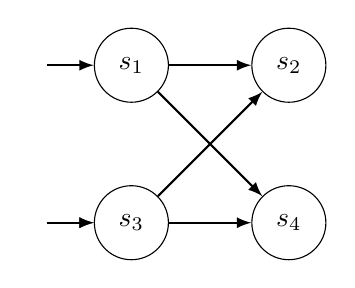
\begin{tikzpicture}
%		\createstate{s1}{3,2+4}{$\state_1$};
		\path 
		(\basex,  \basey+2) node[mstate] (s-1) {$\state_1$} 
		(\basex+3,\basey+2) node[mstate] (s-2) {$\state_2$}
		(\basex,  \basey+0) node[mstate] (s-3) {$\state_3$}
		(\basex+3,\basey+0) node[mstate] (s-4) {$\state_4$}
		(s-1)++(-1.2,0) node (s-1-in) {}
		(s-3)++(-1.2,0) node (s-3-in) {};
	
	
%		midway, at start, near start, very near start, at end, near end, very near end
		
		\path [trans] (s-1) -- (s-2) node [midway, above] () {}; 
		\path [trans] (s-1) -- (s-4);
		\path [trans] (s-3) -- (s-2);
		\path [trans] (s-3) -- (s-4);
		\path [trans] (s-1-in) -- (s-1);
		\path [trans] (s-3-in) -- (s-3);
		\path [trans] (s-3-in) -- (s-3);
		
%		\foreach \x [count=\i] in {midway, at start, near start, very near start, at end, near end, very near end} {
%			\draw (0,-\i) .. controls ++(1,1) and ++(-1,1) .. ++(4,0) node [\x, sloped, fill=white] () {\x};}
%		\draw []
%		\createnode{s2}{}
		
		
		
		
%		\node [draw, circle, fill, scale=0.6] (x1) at (4,7) {};
%		\node [draw, circle, fill, scale=0.6] (x2) at (4,4) {};
%		\node [draw, circle, fill, scale=0.6] (x3) at (4,3) {};
%		\node [draw, circle, fill, scale=0.6] (x4) at (4,0.5) {};
%		
%		\node [label=right:{$v_n$}] at (4.35,7) {};
%		\node [label=right:{$v_{n-h-1}$}] at (4.35,3) {};
%		\node [label=right:{$v_{h+1}$}] at (4.35,0.5) {};
%		
%		\node [draw, circle, fill, scale=0.6, label=left:{$v_h$}] (v1) at (1,7) {};
%		\node [draw, circle, fill, scale=0.6, label=left:{$v_2$}] (v2) at (1,4) {};
%		\node [draw, circle, fill, scale=0.6, label=left:{$v_1$}] (vh) at (1,3) {};
%		
%		\path[thick] (v1) edge (x1);
%		\path[thick] (v2) edge (x2);
%		\path[thick] (v2) edge (x3);
%		\path[thick] (vh) edge (x2);
%		\path[thick] (vh) edge (x3);
%		
%		\node [draw, circle, fill, scale=0.1] (v1) at (1,5.75) {};
%		\node [draw, circle, fill, scale=0.1] (v1) at (1,5.5) {};
%		\node [draw, circle, fill, scale=0.1] (v1) at (1,5.25) {};
%		
%		\node [draw, circle, fill, scale=0.1] (v1) at (4,5.75) {};
%		\node [draw, circle, fill, scale=0.1] (v1) at (4,5.5) {};
%		\node [draw, circle, fill, scale=0.1] (v1) at (4,5.25) {};
%		
%		\node [draw, circle, fill, scale=0.1] (v1) at (4,2) {};
%		\node [draw, circle, fill, scale=0.1] (v1) at (4,1.75) {};
%		\node [draw, circle, fill, scale=0.1] (v1) at (4,1.5) {};
%		
%		\node (y1) at (1.6,6) {};
%		\node (y2) at (3.2,6) {};
%		\node (y3) at (3.2,5) {};
%		\node (y4) at (1.6,5) {};
%		
%		\path (y1) edge (y3);
%		\path (y2) edge (y4);
%		
%		\node (y5) at (1.6,6.2) {};
%		\node (y6) at (3.2,6.2) {};
%		\node (y7) at (3.2,5.2) {};
%		\node (y8) at (1.6,5.2) {};
%		
%		\path (y5) edge (y7);
%		\path (y6) edge (y8);
%		
%		%		\node [label=right:{$K_{h,h}$}] (Khh) at (1.5,2.5) {};
%		\node [label=right:{$K^{n-h}$}] at (4.5,5.5) {};
%		
%		\node [label=right:{$V(G) = \{v_1, v_2, \ldots, v_n\}$}] at (8,5) {};
%		%		\node [label=right:{$E(G) = \{ v_iv_j \mid i,j > h \} \cup \{ v_iv_j \mid i \leq h; j > n-h \}$}] at (7,4) {};
%		\node [label=right:{$E(G) = \{ v_iv_j \mid i,j > h \} \hspace{1mm} \cup$}] at (8,4) {};
%		\node [label=right:{$\{ v_iv_j \mid i \leq h; j > n-h \}$}] at (10.2,3) {};
		
	\end{tikzpicture}
\end{document}
	\end{minipage}%
	\begin{minipage}{.5\textwidth}
		\documentclass[tikz]{standalone}
%\usepackage{prelude}

%%%%%%%%%%%%%%%%%%%%%%%%%%%%%%%%%%%% PACKAGES %%%%%%%%%%%%%%%%%%%%%%%%%%%%%%%%%%%%%%%%%%

\usepackage{inputenc,fontenc}
\usepackage[a4paper,margin=3cm]{geometry}
\usepackage[english]{babel}
%\usepackage[german]{babel}
%\usepackage[fixlanguage]{babelbib}


\usepackage{bbold}
\usepackage{amsthm}
\usepackage{amsmath}
\usepackage{amssymb} % doteqdot
\usepackage[dvipsnames]{xcolor}
\usepackage{standalone}
\usepackage{tikz}[mode=buildnew]
\usepackage{cite}
\usepackage{xspace}
\usepackage{relsize}
\usepackage{mathtools} % mathclap
%\usepackage{MnSymbol}
\usepackage{hyperref}
\usepackage{url}
\usepackage{listings} % for code
\usepackage[T1]{fontenc} %<
\hypersetup{
	colorlinks,
	citecolor=black,
	filecolor=black,
	linkcolor=black,
	urlcolor=black
}
\usepackage{pgfplots}
\pgfplotsset{compat=1.18}
%\usepackage{courier} %% Sets font for listing as Courier. But also for url and texttt!
\usepackage{listings, xcolor}
\usepackage{graphicx}
\usepackage{subcaption}

\usetikzlibrary{calc}
%\usepackage{xparse} % \newDocumentCommand for multiple optional arguments
%\usepackage{titlecaps}



%%%%%%%%%%%%%%%%%%%%%%%%%%%%%%%%%%%% THEOREMSTYLES %%%%%%%%%%%%%%%%%%%%%%%%%%%%%%%%%%

\theoremstyle{definition}
\newtheorem{definition}{Definition}[section]
\newtheorem{exmp}{Beispiel}[section]
%\AfterEndEnvironment{definition}{\noindent\ignorespaces}

\theoremstyle{theorem}
\newtheorem{theorem}{Satz}[section]
\newtheorem{proposition}{Proposition}[section]
%\AfterEndEnvironment{theorem}{\noindent\ignorespaces}

\theoremstyle{korollary}
\newtheorem{korollary}{Korollar}[section]
%\AfterEndEnvironment{korollary}{\noindent\ignorespaces}


\tikzset{
	mstate/.style={draw, circle, minimum size=.94cm}, 
	gstate/.style={draw, rectangle, minimum size=.8cm},
	varstate/.style={draw,rectangle, rounded corners, minimum size=1}, 
	trans/.style={draw, ->, thick},
	bendtrans/.style={draw, ->, thick, bend left=10},
	bendtransr/.style={draw, ->, thick, bend right=10},
	init/.style={initial, initial distance=6pt, initial text=},
	every loop/.style={min distance=5pt, looseness=8},
	>=latex
}
\usetikzlibrary{automata,positioning}

%auto shift/.style={auto=right,->,
%	to path={ let \p1=(\tikztostart),\p2=(\tikztotarget),
%		\n1={atan2(\y2-\y1,\x2-\x1)},\n2={\n1+180}
%		in ($(\tikztostart.{\n1})!1mm!270:(\tikztotarget.{\n2})$) -- 
%		($(\tikztotarget.{\n2})!1mm!90:(\tikztostart.{\n1})$) \tikztonodes}},

%%%%%%%%%%%%%%%%%%%%%%%%%%%%%%%%%%% MY MACROS %%%%%%%%%%%%%%%%%%%%%%%%%%%%%%%%%%%%%%%%%
%formatting
\newcommand{\comment}[2]{{\color{#1}#2}}
\newcommand{\redcomment}[1]{{\color{red}#1}}
\newcommand{\purpcomment}[1]{{\color{pink}#1}}
\newcommand{\bluecomment}[1]{{\color{blue}#1}}
\newcommand{\mt}[1]{\ensuremath{{#1}}\xspace}
\newcommand{\mynewcommand}[2]{\newcommand{#1}{\mt{#2}}} %% currently not used becaue of ide highlighting
\newcommand{\arr}{\mt{\to}}

%model checking terms
\newcommand{\mimicrel}{\mt{\mathcal{R}}}
\newcommand{\bisimeq}{\mt{\;\!\sim\;\!}}
\newcommand{\simorder}{\mt{\;\!\preceq\;\!}}
\newcommand{\simequiv}{\mt{\;\!\simeq\;\!}} %command already defined
\newcommand{\relts}{\mt{\;\!\bullet_{_{\tiny{TS}}}\;\!}}
\newcommand{\rel}{\mt{\;\!\bullet\;\!}}

%own names
\newcommand{\nm}[1]{#1\xspace}
\newcommand{\mdpN}{\nm{MDP}}
\newcommand{\mdpsN}{\nm{MDPs}}
\newcommand{\viewN}{\nm{view}}
\newcommand{\viewNC}{\nm{View}}
\newcommand{\viewsN}{\nm{views}}
\newcommand{\viewsNC}{\nm{Views}}
\newcommand{\grpfctsubN}{\nm{detached grouping function}}
\newcommand{\grpfctsubNC}{\nm{detached grouping function}}
\newcommand{\grpfctsubNCC}{\nm{Detached Grouping Function}}
\newcommand{\grpfctN}{\nm{grouping function}}
\newcommand{\grpfctNC}{\nm{Grouping function}}
\newcommand{\grpfctNCC}{\nm{Grouping Function}}
\newcommand{\grpfctsN}{\nm{grouping functions}}
\newcommand{\grpfctsNC}{\nm{Grouping functions}}
\newcommand{\grpfctsNCC}{\nm{Grouping Functions}}
\newcommand{\stmimicN}{\nm{state-mimic}}
\newcommand{\stmimicsN}{\nm{state-mimics}}
\newcommand{\stmimickingN}{\nm{state-mimicking}}
\newcommand{\stmimickedN}{\nm{state-mimicked}}
%\newcommand{\chosenphtypeNCC}{\nm{Transition System}}
%\newcommand{\chgphNC}{\nm{Transition system}}
%\newcommand{\chgphN}{\nm{transition system}}
%\newcommand{\chgphsNCC}{\nm{Transition Systems}}
%\newcommand{\chgphsNC}{\nm{Transition systems}}
%\newcommand{\chgphsN}{\nm{transition systems}}
\newcommand{\chgphNCC}{\nm{MDP}}
\newcommand{\chgphNC}{\nm{MDP}}
\newcommand{\chgphN}{\nm{MDP}}
\newcommand{\achgphN}{\nm{an MDP}}
\newcommand{\chgphsNCC}{\nm{MDPs}}
\newcommand{\chgphsNC}{\nm{MDPs}}
\newcommand{\chgphsN}{\nm{MDPs}}
\newcommand{\parllcompN}{\nm{parallel composition}}
\newcommand{\parllcompNC}{\nm{Parallel composition}}
\newcommand{\parllcompNCC}{\nm{Parallel Composition}}
\newcommand{\parllcompsN}{\nm{parallel compositions}}
\newcommand{\parllcompsNC}{\nm{Parallel compositions}}
\newcommand{\parllcompsNCC}{\nm{Parallel Compositions}}
\newcommand{\sccN}{\nm{SCC}}
\newcommand{\sccsN}{\nm{SCCs}}
\newcommand{\bsccN}{\nm{BSCC}}
\newcommand{\bsccsN}{\nm{BSCCs}}
\newcommand{\jgrapht}{\nm{jGraphtT}}

\newcommand{\outactident}{\nm{OutActionsIdent}}

%names
\newcommand{\iffN}{\nm{if and only if}}
\newcommand{\tsN}{\nm{TS}}

%% outactions identical
\newcommand{\outactidentstrong}{\nm{strong}}
\newcommand{\outactidentweak}{\nm{weak}}

% CORE DEFINITIONS
\newcommand{\grpfct}[1][\viewppty]{\mt{F_{#1}}}
\newcommand{\grpfctsub}[1][\viewppty]{\mt{\tilde{F}_{#1}}}
%\newcommand{\grpfctimg}[1]{\mt{{\grpfct}[{#1}]}}
%\newcommand{\fctimg}[2]{\mt{{#1}[{#2}]}}
\newcommand{\eqrelview}{\mt{R}}
\newcommand{\eqclassv}[1][\state]{\mt{\eqclass{#1}{\eqrelview}}}
\newcommand{\eqclasssetv}[1][\states]{\mt{{#1}/\eqrelview}} %OLD: \bigcup_{\state \in \states} \eqclassv
\newcommand{\viewid}{\mt{\mdp}}
\newcommand{\view}[1][\viewppty]{\mt{\viewid_{#1}}}
\newcommand{\imggrp}{\mt{\arbset}}
\newcommand{\imggrpsub}{\mt{X}}
\newcommand{\viewppty}{\mt{\theta}}
\newcommand{\pll}{\mt{\;\!\pllpure\;\!}}
\newcommand{\pllrev}{\mt{\pllpure^{-1}}}
\newcommand{\pllpure}{\mt{||}}
\newcommand{\compselectset}{\mt{Z}}
\newcommand{\compselectpure}{\mt{\pllpure_\compselectset}}
\newcommand{\compselect}{\mt{\;\pllpure_\compselectset\;}}
\newcommand{\remstates}{\mt{\bigcup_{\state \in \states \setminus \states_1}\{\{\state\}\}}}
\newcommand{\nogroupstates}[1][\states_2]{\mt{\bigcup_{\state \in \states \setminus {#1}}\{\{\state\}\}}}
\newcommand{\remelem}{\mt{\bullet}}
\newcommand{\nogroupset}{\mt{\xi}}
\newcommand{\remset}{\mt{\{\remelem\}}}
\newcommand{\gfctpll}{\mt{\grpfct[\pll]}}
\newcommand{\group}{\mt{\top}}
\newcommand{\imggrpbinview}{\mt{\{\remelem, \notppty\}}}
\newcommand{\viewappset}{\mt{\tilde{\states}}}
\newcommand{\hasppty}{\mt{\top}}
\newcommand{\notppty}{\mt{\bot}}
\newcommand{\disregardelem}{\mt{\Delta}}
\newcommand{\disregardelements}{\mt{{\disregardelem_1, \dots, \disregardelem_n}}}



%\newcommand{\mdp}{def}\mdp
%\newcommand{\mdpdef}



% EXAMPLE VIEWS
\newcommand{\pptyatomicprops}{\mt{\atomicprops}}
\newcommand{\pptyinitstates}{\mt{\initstates}}
\newcommand{\pptyinactsetsize}{\mt{|\inacts(\state)|}}
\newcommand{\pptyhasoutact}{\mt{\exists\outact}}
\newcommand{\pptyminoutact}[2]{\mt{#1\leq#2}}
\newcommand{\pptymaxoutact}[2]{\mt{#2\leq#1}}
\newcommand{\pptyspanoutact}[3]{\mt{#1\leq#2\leq#3}}
\newcommand{\pptyoutactsetsize}{\mt{|\outacts(\state)|}}
\newcommand{\pptyoutactsingle}{\mt{|\outacts(\state)|_1}}
\newcommand{\pptystrongoutactident}{\mt{\outacts(\state)_=}}
\newcommand{\pptyweakoutactident}{\mt{\outacts(\state)_\approx}}
\newcommand{\pptyhasinact}{\mt{\exists\inact}}
\newcommand{\pptymininact}[2]{\mt{#1\leq#2}}
\newcommand{\pptymaxinact}[2]{\mt{#2\leq#1}}
\newcommand{\pptyspaninact}[3]{\mt{#1\leq#2\leq#3}}
\newcommand{\pptyinactsingle}{\mt{|\inacts(\state)|_1}}
\newcommand{\pptystronginactident}{\mt{\inacts(\state)_=}}
\newcommand{\pptyweakinactident}{\mt{\inacts(\state)_\approx}}
\newcommand{\pptyparamvalueseq}{\mt{\var = \varval}}
\newcommand{\pptyparamvaluesneq}{\mt{\var \neq \varval}}
\newcommand{\pptyparamdnf}{\mt{VarDNF}}
\newcommand{\pptyparamcnf}{\mt{VarCNF}}
\newcommand{\pptyparamvalueseqopt}{\mt{\var = \varval}}
\newcommand{\pptyparamvalident}{\mt{Var:\varval}}
\newcommand{\pptydistance}{\mt{\distpath}}
\newcommand{\pptydistancerev}{\mt{\distpathrev}}
\newcommand{\pptydistancebi}{\mt{\distpathbi}}
\newcommand{\pptyhascycle}{\mt{\exists\cycle}}
\newcommand{\pptyexactactcycle}{\mt{\{\cycle_{\action,n}\}}}
\newcommand{\pptycycleset}{\mt{\cup{\{\state\}_\cycle}}}
\newcommand{\pptyexactcycle}{\mt{\{\cycle_n\}}}
\newcommand{\pptyscc}{\mt{scc}}
\newcommand{\pptybscc}{\mt{bscc}}
\newcommand{\pptyprop}{\mt{\redcomment{?}}}
\newcommand{\pptyident}{id}


\newcommand{\gfctatomicprops}{\mt{\grpfct[\pptyatomicprops]}}
\newcommand{\gfctinitstates}{\mt{\grpfct[\pptyinitstates]^\hasppty}}
\newcommand{\gfcthasoutaction}{\mt{\grpfct[\pptyhasoutact]^\hasppty}}
\newcommand{\gfctminoutaction}{\mt{\grpfct[\pptyminoutact{\numoutact}{\outact}]^\hasppty}}
\newcommand{\gfctmaxoutaction}{\mt{\grpfct[\pptymaxoutact{\numoutact}{\outact}]^\hasppty}}
\newcommand{\gfctspanoutaction}{\mt{\grpfct[\pptyspanoutact{\numoutactb}{\outact}{\numoutact}]^\hasppty}}
\newcommand{\gfctoutactsetsize}{\mt{\grpfct[\pptyoutactsetsize]}}
\newcommand{\gfctoutactsingle}{\mt{\grpfct[\pptyoutactsingle]^\notppty}}
\newcommand{\gfctstrongoutactident}{\mt{\grpfct[\pptystrongoutactident]}}
\newcommand{\gfctweakoutactident}{\mt{\grpfct[\pptyweakoutactident]}}
\newcommand{\gfcthasinaction}{\mt{\grpfct[\pptyhasinact]^\hasppty}}
\newcommand{\gfctmininaction}{\mt{\grpfct[\pptymininact{\numinact}{\inact}]^\hasppty}}
\newcommand{\gfctmaxinaction}{\mt{\grpfct[\pptymaxinact{\numinact}{\inact}]^\hasppty}}
\newcommand{\gfctspaninaction}{\mt{\grpfct[\pptyspaninact{\numinactb}{\inact}{\numinact}]^\hasppty}}
\newcommand{\gfctinactsetsize}{\mt{\grpfct[\pptyinactsetsize]}}
\newcommand{\gfctinactsingle}{\mt{\grpfct[\pptyinactsingle]^\notppty}}
\newcommand{\gfctstronginactident}{\mt{\grpfct[\pptystronginactident]}}
\newcommand{\gfctweakinactident}{\mt{\grpfct[\pptyweakinactident]}}
\newcommand{\gfctparamvalueseq}{\mt{\grpfct[\pptyparamvalueseq]^\hasppty}}
\newcommand{\gfctparamvaluesneq}{\mt{\grpfct[\pptyparamvaluesneq]^\hasppty}}
\newcommand{\gfctparamdnf}{\mt{\grpfct[\pptyparamdnf]^\hasppty}}
\newcommand{\gfctparamcnf}{\mt{\grpfct[\pptyparamcnf]^\hasppty}}
\newcommand{\gfctparamvalueseqopt}{\mt{\pptyparamvalueseqopt}}
\newcommand{\gfctparamvalident}{\mt{\grpfct[\pptyparamvalident]}}
\newcommand{\gfctdistance}{\mt{\grpfct[\pptydistance]}}
\newcommand{\gfctdistancerev}{\mt{\grpfct[\pptydistancerev]}}
\newcommand{\gfctdistancebi}{\mt{\grpfct[\pptydistancebi]}}
\newcommand{\gfcthascycle}{\mt{\grpfct[\pptyhascycle]}}
\newcommand{\gfctexactcycle}{\mt{\grpfct[\pptyexactcycle]}}
\newcommand{\gfctcycleset}{\mt{\grpfct[\pptycycleset]}}
\newcommand{\gfctexactactcycle}{\mt{\grpfct[\pptyexactactcycle]}}
\newcommand{\gfctscc}{\mt{\grpfct[\pptyscc]}}
\newcommand{\gfctbscc}{\mt{\grpfct[\pptybscc]}}
\newcommand{\gfctprop}{\mt{\grpfct[\pptyprop]}}
\newcommand{\gfctident}{\mt{\grpfct[\pptyident]}}

\newcommand{\gfctsubatomicprops}{\mt{\grpfctsub[\pptyatomicprops]}}
\newcommand{\gfctsubinitstates}{\mt{\grpfctsub[\pptyinitstates]^\hasppty}}
\newcommand{\gfctsubhasoutaction}{\mt{\grpfctsub[\pptyhasoutact]^\hasppty}}
\newcommand{\gfctsubminoutaction}{\mt{\grpfctsub[\pptyminoutact{\numoutact}{\outact}]^\hasppty}}
\newcommand{\gfctsubmaxoutaction}{\mt{\grpfctsub[\pptymaxoutact{\numoutact}{\outact}]^\hasppty}}
\newcommand{\gfctsubspanoutaction}{\mt{\grpfctsub[\pptyspanoutact{\numoutactb}{\outact}{\numoutact}]^\hasppty}}
\newcommand{\gfctsuboutactsetsize}{\mt{\grpfctsub[\pptyoutactsetsize]}}
\newcommand{\gfctsuboutactsingle}{\mt{\grpfctsub[\pptyoutactsingle]^\notppty}}
\newcommand{\gfctsubstrongoutactident}{\mt{\grpfctsub[\pptystrongoutactident]^\hasppty}}
\newcommand{\gfctsubweakoutactident}{\mt{\grpfctsub[\pptyweakoutactident]^\hasppty}}
\newcommand{\gfctsubhasinaction}{\mt{\grpfctsub[\pptyhasinact]}}
\newcommand{\gfctsubmininaction}{\mt{\grpfctsub[\pptymininact{\numinact}{\inact}]}}
\newcommand{\gfctsubmaxinaction}{\mt{\grpfctsub[\pptymaxinact{\numinact}{\inact}]}}
\newcommand{\gfctsubspaninaction}{\mt{\grpfctsub[\pptyspaninact{\numinactb}{\inact}{\numinact}]}}
\newcommand{\gfctsubinactsetsize}{\mt{\grpfctsub[\pptyinactsetsize]^\hasppty}}
\newcommand{\gfctsubinactsingle}{\mt{\grpfctsub[\pptyinactsingle]^\notppty}}
\newcommand{\gfctsubstronginactident}{\mt{\grpfctsub[\pptystronginactident]}}
\newcommand{\gfctsubweakinactident}{\mt{\grpfctsub[\pptyweakinactident]}}
\newcommand{\gfctsubparamvalueseq}{\mt{\grpfctsub[\pptyparamvalueseq]^\hasppty}}
\newcommand{\gfctsubparamvaluesneq}{\mt{\grpfctsub[\pptyparamvaluesneq]^\hasppty}}
\newcommand{\gfctsubparamdnf}{\mt{\grpfctsub[\pptyparamdnf]^\hasppty}}
\newcommand{\gfctsubparamcnf}{\mt{\grpfctsub[\pptyparamcnf]^\hasppty}}
\newcommand{\gfctsubparamvalueseqopt}{\mt{\pptyparamvalueseqopt}}
\newcommand{\gfctsubparamvalident}{\mt{\grpfctsub[\pptyparamvalident]}}
\newcommand{\gfctsubdistance}{\mt{\grpfctsub[\pptydistance]}}
\newcommand{\gfctsubdistancerev}{\mt{\grpfctsub[\pptydistancerev]}}
\newcommand{\gfctsubdistancebi}{\mt{\grpfctsub[\pptydistancebi]}}
\newcommand{\gfctsubhascycle}{\mt{\grpfctsub[\pptyhascycle]^\hasppty}}
\newcommand{\gfctsubexactcycle}{\mt{\grpfctsub[\pptyexactcycle]}}
\newcommand{\gfctsubcycleset}{\mt{\grpfctsub[\pptycycleset]}}
\newcommand{\gfctsubexactactcycle}{\mt{\grpfctsub[\pptyexactactcycle]}}
\newcommand{\gfctsubscc}{\mt{\grpfctsub[\pptyscc]}}
\newcommand{\gfctsubbscc}{\mt{\grpfctsub[\pptybscc]}}
\newcommand{\gfctsubprop}{\mt{\grpfctsub[\pptyprop]}}
\newcommand{\gfctsubident}{\mt{\grpfctsub[\pptyident]}}


\newcommand{\viewatomicprops}{\mt{\view[\pptyatomicprops]}}
\newcommand{\viewinitstates}{\mt{\view[\pptyinitstates]^\hasppty}}
\newcommand{\viewhasoutaction}{\mt{\view[\pptyhasoutact]^\hasppty}}
\newcommand{\viewminoutaction}{\mt{\view[\pptyminoutact{\numoutact}{\outact}]^\hasppty}}
\newcommand{\viewmaxoutaction}{\mt{\view[\pptymaxoutact{\numoutact}{\outact}]^\hasppty}}
\newcommand{\viewspanoutaction}{\mt{\view[\pptyspanoutact{\numoutactb}{\outact}{\numoutact}]^\hasppty}}
\newcommand{\viewoutactsetsize}{\mt{\view[\pptyoutactsetsize]}}
\newcommand{\viewoutactsingle}{\mt{\view[\pptyoutactsingle]^\notppty}}
\newcommand{\viewstrongoutactident}{\mt{\view[\pptystrongoutactident]}}
\newcommand{\viewweakoutactident}{\mt{\view[\pptyweakoutactident]}}
\newcommand{\viewhasinaction}{\mt{\view[\pptyhasinact]^\hasppty}}
\newcommand{\viewmininaction}{\mt{\view[\pptymininact{\numinact}{\inact}]^\hasppty}}
\newcommand{\viewmaxinaction}{\mt{\view[\pptymaxinact{\numinact}{\inact}]^\hasppty}}
\newcommand{\viewspaninaction}{\mt{\view[\pptyspaninact{\numinactb}{\inact}{\numinact}]^\hasppty}}
\newcommand{\viewinactsetsize}{\mt{\view[\pptyinactsetsize]}}
\newcommand{\viewinactsingle}{\mt{\view[\pptyinactsingle]^\notppty}}
\newcommand{\viewstronginactident}{\mt{\view[\pptystronginactident]}}
\newcommand{\viewweakinactident}{\mt{\view[\pptyweakinactident]}}
\newcommand{\viewparamvalueseq}{\mt{\view[\pptyparamvalueseq]}}
\newcommand{\viewparamvaluesneq}{\mt{\view[\pptyparamvaluesneq]}}
\newcommand{\viewparamdnf}{\mt{\view[\pptyparamdnf]^\hasppty}}
\newcommand{\viewparamcnf}{\mt{\view[\pptyparamcnf]^\hasppty}}
\newcommand{\viewparamvalueseqopt}{\mt{\pptyparamvalueseqopt}}
\newcommand{\viewparamvalident}{\mt{\view[\pptyparamvalident]}}
\newcommand{\viewdistance}{\mt{\view[\pptydistance]}}
\newcommand{\viewdistancerev}{\mt{\view[\pptydistancerev]}}
\newcommand{\viewdistancebi}{\mt{\view[\pptydistancebi]}}
\newcommand{\viewhascycle}{\mt{\view[\pptyhascycle]}}
\newcommand{\viewexactcycle}{\mt{\view[\pptyexactcycle]}}
\newcommand{\viewcycleset}{\mt{\view[\pptycycleset]}}
\newcommand{\viewexactactcycle}{\mt{\view[\pptyexactactcycle]}}
\newcommand{\viewscc}{\mt{\view[\pptyscc]}}
\newcommand{\viewbscc}{\mt{\view[\pptybscc]}}
\newcommand{\viewprop}{\mt{\view[\pptyprop]}}
\newcommand{\viewident}{\mt{\view[\pptyident]}}

%\newcommand{\viewatomicprops}{\mt{\view[\atomicprops]}}
%\newcommand{\viewinitstates}{\mt{\view[\initstates]}}
%\newcommand{\viewhasoutaction}{\mt{\view[\pptyhasoutact]}}
%\newcommand{\viewminoutaction}{\mt{\view[\pptyminoutact{\numoutact}{\outact}]}}
%\newcommand{\viewmaxoutaction}{\mt{\view[\pptymaxoutact{\numoutact}{\outact}]}}
%\newcommand{\viewspanoutaction}{\mt{\view[\pptyspanoutact{\numoutactb}{\outact}{\numoutact}]}}
%\newcommand{\viewoutactsetsize}{\mt{\view[\pptyoutactsetsize]}}
%\newcommand{\viewoutactsingle}{\mt{\view[\pptyoutactsingle]}}
%\newcommand{\viewstrongoutactident}{\mt{\view[\outacts(\state)_=]}}
%\newcommand{\viewweakoutactident}{\mt{\view[\outacts(\state)_\approx]}}
%\newcommand{\viewhasinaction}{\mt{\view[\pptyhasinact]}}
%\newcommand{\viewmininaction}{\mt{\view[\pptymininact{\numinact}{\inact}]}}
%\newcommand{\viewmaxinaction}{\mt{\view[\pptymaxinact{\numinact}{\inact}]}}
%\newcommand{\viewspaninaction}{\mt{\view[\pptyspaninact{\numinactb}{\inact}{\numinact}]}}
%\newcommand{\viewinactsetsize}{\mt{\view[\pptyinactsetsize]}}
%\newcommand{\viewinactsingle}{\mt{\view[\pptyinactsingle]}}
%\newcommand{\viewstronginactident}{\mt{\view[\inacts(\state)_=]}}
%\newcommand{\viewweakinactident}{\mt{\view[\inacts(\state)_\approx]}}
%\newcommand{\viewparamvalueseq}{\mt{\view[\var = \varval]}}
%\newcommand{\viewparamvaluesneq}{\mt{\view[\var \neq \varval]}}
%\newcommand{\viewparamdnf}{\mt{\view[VarDNF]}}
%\newcommand{\viewparamcnf}{\mt{\view[VarCNF]}}
%\newcommand{\viewparamvalident}{\mt{\view[\pptyparamvalident]}}
%\newcommand{\viewdistance}{\mt{\view[\pptydistance]}}
%\newcommand{\viewhascycle}{\mt{\view[\exists\cycle]}}
%\newcommand{\viewexactcycle}{\mt{\view[\pptyexactcycle]}}
%\newcommand{\viewcycleset}{\mt{\view[\pptycycleset]}}
%\newcommand{\viewexactactcycle}{\mt{\view[\pptyexactactcycle]}}
%\newcommand{\viewscc}{\mt{\view[scc]}}
%\newcommand{\viewbscc}{\mt{\view[bscc]}}

%actions
\newcommand{\numoutact}{\mt{n}}
\newcommand{\numoutactb}{\mt{m}}
\newcommand{\numinact}{\mt{n}}
\newcommand{\numinactb}{\mt{m}}

\newcommand{\predmaxoutact}[1][\numoutact]{\mt{Q_{\outact\leq#1}(\state,\state_1, \dots, \state_{#1+1})}}
\newcommand{\predminoutact}[1][\numoutact]{\mt{Q_{#1\leq\outact}(\state,\state_1, \dots, \state_{#1})}}
\newcommand{\formoutact}[1][\state]{\mt{C_{#1,\outact}}}
\newcommand{\predmaxinact}[1][\numinact]{\mt{Q_{\inact\leq#1}(\state,\state_1, \dots, \state_{#1+1})}}
\newcommand{\predmininact}[1][\numinact]{\mt{Q_{#1\leq\inact}(\state,\state_1, \dots, \state_{#1})}}

\newcommand{\outact}[1][\action]{\mt{\overrightarrow{#1}}}
\newcommand{\outacts}{\mt{\overrightarrow{\actions}}}
\newcommand{\inact}{\mt{\overleftarrow{\action}}}
\newcommand{\inacts}[1][\action]{\mt{\overleftarrow{#1}}}

%%Parameters
\newcommand{\vars}[1][\mdp]{\mt{V\!ar_{#1}}}
\newcommand{\var}{\mt{x}}
\newcommand{\varstate}[1][]{\mt{\var_{\state#1}}}
\newcommand{\varval}{\mt{a}}
\newcommand{\vareval}[1][\mdp]{\mt{V\!arEval_{#1}}}
\newcommand{\varevalimg}[1][\mdp]{\mt{\vareval[#1][\states,\vars]}}
\newcommand{\varevalimgset}{\mt{\arbset}}
\newcommand{\someparam}{\mt{\tilde{x}}}
\newcommand{\eqorneq}{\mt{\;\doteqdot\;}}
\newcommand{\varstyle}[2]{\mt{\langle#1,#2\rangle}}




%\makeatletter
%\newcommand{\overleftrightsmallarrow}{\mathpalette{\overarrowsmall@\leftrightarrowfill@}}
%\newcommand{\overrightsmallarrow}{\mathpalette{\overarrowsmall@\rightarrowfill@}}
%\newcommand{\overleftsmallarrow}{\mathpalette{\overarrowsmall@\leftarrowfill@}}
%\newcommand{\overarrowsmall@}[3]{%
%	\vbox{%
%		\ialign{%
%			##\crcr
%			#1{\smaller@style{#2}}\crcr
%			\noalign{\nointerlineskip}%
%			$\m@th\hfil#2#3\hfil$\crcr
%		}%
%	}%
%}
%\def\smaller@style#1{%
%	\ifx#1\displaystyle\scriptstyle\else
%	\ifx#1\textstyle\scriptstyle\else
%	\scriptscriptstyle
%	\fi
%	\fi
%}
%\makeatother
%\newcommand{\te}[1]{\overleftrightsmallarrow{#1}}

% Distance
\newcommand{\fctdist}{\mt{distance}}
\newcommand{\fctdistdefault}{\mt{\fctdist(\chgph, \smstates, \grandist)}}
\newcommand{\distval}{\mt{d}}
\newcommand{\grandist}{\mt{n}}
\let\path\oldpath
\newcommand{\path}{\mt{P}}
\newcommand{\pathbi}{\mt{\bar{\path}}}
\newcommand{\pathsecfull}{\mt{(\state_0, \action_0, \state_1, \action_1, \dots, \action_{n}, \state_{n+1})}}
\newcommand{\lenpath}{\mt{len}}
\newcommand{\pfirst}{\mt{first}}
\newcommand{\plast}{\mt{last}}
\newcommand{\pathset}{\mt{\path_\chgph}}
\newcommand{\pathbiset}{\mt{\pathbi_\chgph}}
\newcommand{\distpath}{\mt{\overrightarrow{dist}}}
\newcommand{\distpathrev}{\mt{\overleftarrow{dist}}}
\newcommand{\distpathbi}{\mt{\overline{dist}}}
%Cycles
\newcommand{\cyclesecfull}{\mt{(\state_0, \action_0, \state_1, \action_1, \dots, \action_{n-1}, \state_0)}}
\newcommand{\fctfindcycles}{\mt{findCycles}}
\newcommand{\cycle}{\mt{C}}
\newcommand{\cycleset}{\mt{\cycle_{\mdp, n}}}
\newcommand{\lencycle}{\mt{len}}
% strongly connected components
\newcommand{\scc}{\mt{T}}
\newcommand{\setscc}{\mt{SCC_{\chgph,n}}}
\newcommand{\setbscc}{\mt{BSCC_{\chgph,n}}}

% properties
\newcommand{\propfct}{\mt{f}}

% all Systems
\newcommand{\chgph}{\mt{\mdp}}
\newcommand{\chgphtuple}{\mt{\mdptuple}}
\newcommand{\chgphtupledist}{\mt{\mdptupledist}}

\newcommand{\states}{\mt{S}}
\newcommand{\actions}{\mt{Act}}
\newcommand{\atomicprops}{\mt{AP}}
\newcommand{\labelingfct}{\mt{L}}
\newcommand{\init}{\mt{\initdistrib}} % use MDP % refers to the underlying set
\newcommand{\trans}{\mt{\probtfunc}} % use MDP % refers to the underlying set
\newcommand{\smstates}{\mt{\tilde{\states}}}


\newcommand{\state}{\mt{s}}
\newcommand{\action}{\mt{\alpha}}
\newcommand{\actionb}{\mt{\beta}}
\newcommand{\actionc}{\mt{\gamma}}
\newcommand{\smstate}{\mt{\tilde{\state}}}



% transition sysstems
\newcommand{\ts}{\mt{TS}}
\newcommand{\transitionrel}{\mt{\longrightarrow}}
\newcommand{\initstates}{\mt{I}}
\newcommand{\transitionsystem}{\mt
	{(\states, \actions, \transitionrel, \initstates, \atomicprops, \labelingfct)}
}
\newcommand{\tstupledist}{\mt{(\states', \actions',\transitionrel', \initstates', \labelingfct')}}


%Markov chains and MDP
\newcommand{\mdp}{\mt{\autm}}
\newcommand{\mdptuple}{\mt{(\states, \actions, \probtfunc, \initdistrib, \atomicprops, \labelingfct)}}
\newcommand{\mdptupledist}{\mt{(\states', \actions', \probtfunc', \initdistrib', \atomicprops', \labelingfct')}}
\newcommand{\autm}{\mt{\mathcal{M}}}
\newcommand{\probtfunc}{\mt{\textbf{P}}}
\newcommand{\initdistrib}{\mt{\iota_{init}}}


%maths
\newcommand{\powerset}[1]{\mt{\mathcal{P}(#1)}}
\newcommand{\eqclass}[2]{\mt{[#1]_{#2}}}%{\mt{#1 / #2}}
\newcommand{\impr}{\mt{\hspace{3mm}\Rightarrow\hspace{2mm}}}
\newcommand{\impl}{\mt{\hspace{3mm}\Leftarrow\hspace{2mm}}}
\newcommand{\natnums}{\mt{\mathbb{N}}} 
\newcommand{\realnums}{\mt{\mathbb{R}}}
\newcommand{\intmodn}[1][n]{\mt{\mathbb{Z}_{#1}}}
\newcommand{\arbset}{\mt{M}}
\newcommand{\bigsum}[2][]{\mt{\mathlarger{\sum}_{#2}^{#1}}}
\newcommand{\bbigsum}[2][]{\mt{\mathlarger{\mathlarger{\sum}}_{#2}^{#1}}}
\newcommand{\invimage}[2]{#1^{\mt{-1}(#2)}}
\newcommand{\img}{\mt{Img}}
\newcommand{\cond}{\mt{\,|\,}}

%tickz
%% \definecolor{darkred}{RGB}{196, 42, 42}

%implementation
\newcommand{\pmcvis}{\nm{PMC-Vis}}


\usepackage{tikz}


\begin{document}
	\newcommand{\createstate}[3]{\node[draw, circle, minimum size=1cm] (#1) at (#2) {#3}}
	\newcommand{\basex}{0}
	\newcommand{\basey}{0}
	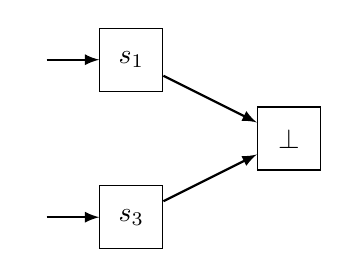
\begin{tikzpicture}
		%		\createstate{s1}{3,2+4}{$\state_1$};
		\path 
		(\basex,  \basey+2) node[gstate] (s-1) {$\state_1$} 
		(\basex,  \basey+0) node[gstate] (s-3) {$\state_3$}
		(\basex+3,\basey+1) node[gstate] (s-bot) {$\bot$}
		(s-1)++(-1.2,0) node (s-1-in) {}
		(s-3)++(-1.2,0) node (s-3-in) {};
		
		
		%		midway, at start, near start, very near start, at end, near end, very near end
		
		\path [trans] (s-1) -- (s-bot);
		\path [trans] (s-3) -- (s-bot);
		\path [trans] (s-1-in) -- (s-1);
		\path [trans] (s-3-in) -- (s-3);
		
		
	\end{tikzpicture}
\end{document}
	\end{minipage}
	\caption{Simplified representations of \mdp (left) and the \viewN \viewinitstates on it (right)}
	\label{fig:initStatesExmp}  
\end{figure}


\subsubsection{Outgoing Actions}
Another crucial component of \achgphN is its set of actions \actions. Actions are used for interprocesscommunication und synchronization. In this subsection we will provide and dicuss some views utilizing actions on transitions that are outgonig from a state. 
%For simplicity we will write "outgoing action \action" short for "transition with outgoing action \action" analogously we will write "ingoing action \action" short for "transition with ingoing action \action". We
We will write a state \state has an outgoing action \action if there exists a state $\state'$ with $(\state, \action, \state') \in \trans$. For a state \state, ingoing action \action we say it has an ingoing action \action if there exist a state $\state'$ with $(\state', \action, \state) \in \trans$.

The most obvious variant to group states is to group states that \emph{have} a given outgoing action.

\begin{definition}
	Let $\chgph = \chgphtuple$ be \achgphN and $\action \in \actions$. The view \viewhasoutaction is defined by its \grpfctN $\gfcthasoutaction : \states \to \imggrp$ with 
	
	\[
	\state \mapsto
	\begin{cases}
			\group,				& \text{if } \exists \state' \in \states: (\state, \action, \state') \in \trans \\
			\remelem,          	& \text{otherwise}
		\end{cases}
	\]
	
	and $\imggrp := \imggrpbinview$. %\actions \cup \remset$.	
\end{definition}


For $\state_1,\state_2 \in \states$ it is $\gfcthasoutaction(\state_1) = \gfcthasoutaction(\state_2)$ \iffN 
there exist $\state_{a},\state_{b} \in \states$ with 
$(\state_1, \action, \state_{a}), (\state_2, \action, \state_{b}) \in \trans$ (i.e. they have the same outgoing action \action) or $\state_1 = \state_2$. 
In accordance with Definition \ref{def:eqrelview} it is
\begin{align*}
	\eqclassv &= \{\state \in \states \mid \gfcthasoutaction(\state) = \action\} &\exists\state' \in \states : (\state, \action, \state') \in \trans \\
	\eqclassv &= \{\state \in \states \mid \gfcthasoutaction(\state) = \state\} = \{s\} &\text{ otherwise}
\end{align*}
 %if for all $\state' \in \states : (\state,\action,\state') \notin \trans$.

Thereby we obtain the \viewN \viewhasoutaction for a given \chgphN \chgph where $\states' = \bigcup_{\state \in \states} \{\eqclassv\} =: \states_1 \cup \states_2$ where
\begin{align*}
	 \states_1 &:= \{\state \in \states \mid \exists \state' \in \states: (\state, \action, \state') \in \trans\} = \{\state \in \states \mid \state \text{ has outgoing action \action }\} \\
	\states_2 &:= \remstates.
\end{align*}

\begin{figure}[h]
	\begin{minipage}{.5\textwidth}
		\hspace{5mm}
		\documentclass[tikz,preview]{standalone}
%\usepackage{prelude}

%%%%%%%%%%%%%%%%%%%%%%%%%%%%%%%%%%%% PACKAGES %%%%%%%%%%%%%%%%%%%%%%%%%%%%%%%%%%%%%%%%%%

\usepackage{inputenc,fontenc}
\usepackage[a4paper,margin=3cm]{geometry}
\usepackage[english]{babel}
%\usepackage[german]{babel}
%\usepackage[fixlanguage]{babelbib}


\usepackage{bbold}
\usepackage{amsthm}
\usepackage{amsmath}
\usepackage{amssymb} % doteqdot
\usepackage[dvipsnames]{xcolor}
\usepackage{standalone}
\usepackage{tikz}[mode=buildnew]
\usepackage{cite}
\usepackage{xspace}
\usepackage{relsize}
\usepackage{mathtools} % mathclap
%\usepackage{MnSymbol}
\usepackage{hyperref}
\usepackage{url}
\usepackage{listings} % for code
\usepackage[T1]{fontenc} %<
\hypersetup{
	colorlinks,
	citecolor=black,
	filecolor=black,
	linkcolor=black,
	urlcolor=black
}
\usepackage{pgfplots}
\pgfplotsset{compat=1.18}
%\usepackage{courier} %% Sets font for listing as Courier. But also for url and texttt!
\usepackage{listings, xcolor}
\usepackage{graphicx}
\usepackage{subcaption}

\usetikzlibrary{calc}
%\usepackage{xparse} % \newDocumentCommand for multiple optional arguments
%\usepackage{titlecaps}



%%%%%%%%%%%%%%%%%%%%%%%%%%%%%%%%%%%% THEOREMSTYLES %%%%%%%%%%%%%%%%%%%%%%%%%%%%%%%%%%

\theoremstyle{definition}
\newtheorem{definition}{Definition}[section]
\newtheorem{exmp}{Beispiel}[section]
%\AfterEndEnvironment{definition}{\noindent\ignorespaces}

\theoremstyle{theorem}
\newtheorem{theorem}{Satz}[section]
\newtheorem{proposition}{Proposition}[section]
%\AfterEndEnvironment{theorem}{\noindent\ignorespaces}

\theoremstyle{korollary}
\newtheorem{korollary}{Korollar}[section]
%\AfterEndEnvironment{korollary}{\noindent\ignorespaces}


\tikzset{
	mstate/.style={draw, circle, minimum size=.94cm}, 
	gstate/.style={draw, rectangle, minimum size=.8cm},
	varstate/.style={draw,rectangle, rounded corners, minimum size=1}, 
	trans/.style={draw, ->, thick},
	bendtrans/.style={draw, ->, thick, bend left=10},
	bendtransr/.style={draw, ->, thick, bend right=10},
	init/.style={initial, initial distance=6pt, initial text=},
	every loop/.style={min distance=5pt, looseness=8},
	>=latex
}
\usetikzlibrary{automata,positioning}

%auto shift/.style={auto=right,->,
%	to path={ let \p1=(\tikztostart),\p2=(\tikztotarget),
%		\n1={atan2(\y2-\y1,\x2-\x1)},\n2={\n1+180}
%		in ($(\tikztostart.{\n1})!1mm!270:(\tikztotarget.{\n2})$) -- 
%		($(\tikztotarget.{\n2})!1mm!90:(\tikztostart.{\n1})$) \tikztonodes}},

%%%%%%%%%%%%%%%%%%%%%%%%%%%%%%%%%%% MY MACROS %%%%%%%%%%%%%%%%%%%%%%%%%%%%%%%%%%%%%%%%%
%formatting
\newcommand{\comment}[2]{{\color{#1}#2}}
\newcommand{\redcomment}[1]{{\color{red}#1}}
\newcommand{\purpcomment}[1]{{\color{pink}#1}}
\newcommand{\bluecomment}[1]{{\color{blue}#1}}
\newcommand{\mt}[1]{\ensuremath{{#1}}\xspace}
\newcommand{\mynewcommand}[2]{\newcommand{#1}{\mt{#2}}} %% currently not used becaue of ide highlighting
\newcommand{\arr}{\mt{\to}}

%model checking terms
\newcommand{\mimicrel}{\mt{\mathcal{R}}}
\newcommand{\bisimeq}{\mt{\;\!\sim\;\!}}
\newcommand{\simorder}{\mt{\;\!\preceq\;\!}}
\newcommand{\simequiv}{\mt{\;\!\simeq\;\!}} %command already defined
\newcommand{\relts}{\mt{\;\!\bullet_{_{\tiny{TS}}}\;\!}}
\newcommand{\rel}{\mt{\;\!\bullet\;\!}}

%own names
\newcommand{\nm}[1]{#1\xspace}
\newcommand{\mdpN}{\nm{MDP}}
\newcommand{\mdpsN}{\nm{MDPs}}
\newcommand{\viewN}{\nm{view}}
\newcommand{\viewNC}{\nm{View}}
\newcommand{\viewsN}{\nm{views}}
\newcommand{\viewsNC}{\nm{Views}}
\newcommand{\grpfctsubN}{\nm{detached grouping function}}
\newcommand{\grpfctsubNC}{\nm{detached grouping function}}
\newcommand{\grpfctsubNCC}{\nm{Detached Grouping Function}}
\newcommand{\grpfctN}{\nm{grouping function}}
\newcommand{\grpfctNC}{\nm{Grouping function}}
\newcommand{\grpfctNCC}{\nm{Grouping Function}}
\newcommand{\grpfctsN}{\nm{grouping functions}}
\newcommand{\grpfctsNC}{\nm{Grouping functions}}
\newcommand{\grpfctsNCC}{\nm{Grouping Functions}}
\newcommand{\stmimicN}{\nm{state-mimic}}
\newcommand{\stmimicsN}{\nm{state-mimics}}
\newcommand{\stmimickingN}{\nm{state-mimicking}}
\newcommand{\stmimickedN}{\nm{state-mimicked}}
%\newcommand{\chosenphtypeNCC}{\nm{Transition System}}
%\newcommand{\chgphNC}{\nm{Transition system}}
%\newcommand{\chgphN}{\nm{transition system}}
%\newcommand{\chgphsNCC}{\nm{Transition Systems}}
%\newcommand{\chgphsNC}{\nm{Transition systems}}
%\newcommand{\chgphsN}{\nm{transition systems}}
\newcommand{\chgphNCC}{\nm{MDP}}
\newcommand{\chgphNC}{\nm{MDP}}
\newcommand{\chgphN}{\nm{MDP}}
\newcommand{\achgphN}{\nm{an MDP}}
\newcommand{\chgphsNCC}{\nm{MDPs}}
\newcommand{\chgphsNC}{\nm{MDPs}}
\newcommand{\chgphsN}{\nm{MDPs}}
\newcommand{\parllcompN}{\nm{parallel composition}}
\newcommand{\parllcompNC}{\nm{Parallel composition}}
\newcommand{\parllcompNCC}{\nm{Parallel Composition}}
\newcommand{\parllcompsN}{\nm{parallel compositions}}
\newcommand{\parllcompsNC}{\nm{Parallel compositions}}
\newcommand{\parllcompsNCC}{\nm{Parallel Compositions}}
\newcommand{\sccN}{\nm{SCC}}
\newcommand{\sccsN}{\nm{SCCs}}
\newcommand{\bsccN}{\nm{BSCC}}
\newcommand{\bsccsN}{\nm{BSCCs}}
\newcommand{\jgrapht}{\nm{jGraphtT}}

\newcommand{\outactident}{\nm{OutActionsIdent}}

%names
\newcommand{\iffN}{\nm{if and only if}}
\newcommand{\tsN}{\nm{TS}}

%% outactions identical
\newcommand{\outactidentstrong}{\nm{strong}}
\newcommand{\outactidentweak}{\nm{weak}}

% CORE DEFINITIONS
\newcommand{\grpfct}[1][\viewppty]{\mt{F_{#1}}}
\newcommand{\grpfctsub}[1][\viewppty]{\mt{\tilde{F}_{#1}}}
%\newcommand{\grpfctimg}[1]{\mt{{\grpfct}[{#1}]}}
%\newcommand{\fctimg}[2]{\mt{{#1}[{#2}]}}
\newcommand{\eqrelview}{\mt{R}}
\newcommand{\eqclassv}[1][\state]{\mt{\eqclass{#1}{\eqrelview}}}
\newcommand{\eqclasssetv}[1][\states]{\mt{{#1}/\eqrelview}} %OLD: \bigcup_{\state \in \states} \eqclassv
\newcommand{\viewid}{\mt{\mdp}}
\newcommand{\view}[1][\viewppty]{\mt{\viewid_{#1}}}
\newcommand{\imggrp}{\mt{\arbset}}
\newcommand{\imggrpsub}{\mt{X}}
\newcommand{\viewppty}{\mt{\theta}}
\newcommand{\pll}{\mt{\;\!\pllpure\;\!}}
\newcommand{\pllrev}{\mt{\pllpure^{-1}}}
\newcommand{\pllpure}{\mt{||}}
\newcommand{\compselectset}{\mt{Z}}
\newcommand{\compselectpure}{\mt{\pllpure_\compselectset}}
\newcommand{\compselect}{\mt{\;\pllpure_\compselectset\;}}
\newcommand{\remstates}{\mt{\bigcup_{\state \in \states \setminus \states_1}\{\{\state\}\}}}
\newcommand{\nogroupstates}[1][\states_2]{\mt{\bigcup_{\state \in \states \setminus {#1}}\{\{\state\}\}}}
\newcommand{\remelem}{\mt{\bullet}}
\newcommand{\nogroupset}{\mt{\xi}}
\newcommand{\remset}{\mt{\{\remelem\}}}
\newcommand{\gfctpll}{\mt{\grpfct[\pll]}}
\newcommand{\group}{\mt{\top}}
\newcommand{\imggrpbinview}{\mt{\{\remelem, \notppty\}}}
\newcommand{\viewappset}{\mt{\tilde{\states}}}
\newcommand{\hasppty}{\mt{\top}}
\newcommand{\notppty}{\mt{\bot}}
\newcommand{\disregardelem}{\mt{\Delta}}
\newcommand{\disregardelements}{\mt{{\disregardelem_1, \dots, \disregardelem_n}}}



%\newcommand{\mdp}{def}\mdp
%\newcommand{\mdpdef}



% EXAMPLE VIEWS
\newcommand{\pptyatomicprops}{\mt{\atomicprops}}
\newcommand{\pptyinitstates}{\mt{\initstates}}
\newcommand{\pptyinactsetsize}{\mt{|\inacts(\state)|}}
\newcommand{\pptyhasoutact}{\mt{\exists\outact}}
\newcommand{\pptyminoutact}[2]{\mt{#1\leq#2}}
\newcommand{\pptymaxoutact}[2]{\mt{#2\leq#1}}
\newcommand{\pptyspanoutact}[3]{\mt{#1\leq#2\leq#3}}
\newcommand{\pptyoutactsetsize}{\mt{|\outacts(\state)|}}
\newcommand{\pptyoutactsingle}{\mt{|\outacts(\state)|_1}}
\newcommand{\pptystrongoutactident}{\mt{\outacts(\state)_=}}
\newcommand{\pptyweakoutactident}{\mt{\outacts(\state)_\approx}}
\newcommand{\pptyhasinact}{\mt{\exists\inact}}
\newcommand{\pptymininact}[2]{\mt{#1\leq#2}}
\newcommand{\pptymaxinact}[2]{\mt{#2\leq#1}}
\newcommand{\pptyspaninact}[3]{\mt{#1\leq#2\leq#3}}
\newcommand{\pptyinactsingle}{\mt{|\inacts(\state)|_1}}
\newcommand{\pptystronginactident}{\mt{\inacts(\state)_=}}
\newcommand{\pptyweakinactident}{\mt{\inacts(\state)_\approx}}
\newcommand{\pptyparamvalueseq}{\mt{\var = \varval}}
\newcommand{\pptyparamvaluesneq}{\mt{\var \neq \varval}}
\newcommand{\pptyparamdnf}{\mt{VarDNF}}
\newcommand{\pptyparamcnf}{\mt{VarCNF}}
\newcommand{\pptyparamvalueseqopt}{\mt{\var = \varval}}
\newcommand{\pptyparamvalident}{\mt{Var:\varval}}
\newcommand{\pptydistance}{\mt{\distpath}}
\newcommand{\pptydistancerev}{\mt{\distpathrev}}
\newcommand{\pptydistancebi}{\mt{\distpathbi}}
\newcommand{\pptyhascycle}{\mt{\exists\cycle}}
\newcommand{\pptyexactactcycle}{\mt{\{\cycle_{\action,n}\}}}
\newcommand{\pptycycleset}{\mt{\cup{\{\state\}_\cycle}}}
\newcommand{\pptyexactcycle}{\mt{\{\cycle_n\}}}
\newcommand{\pptyscc}{\mt{scc}}
\newcommand{\pptybscc}{\mt{bscc}}
\newcommand{\pptyprop}{\mt{\redcomment{?}}}
\newcommand{\pptyident}{id}


\newcommand{\gfctatomicprops}{\mt{\grpfct[\pptyatomicprops]}}
\newcommand{\gfctinitstates}{\mt{\grpfct[\pptyinitstates]^\hasppty}}
\newcommand{\gfcthasoutaction}{\mt{\grpfct[\pptyhasoutact]^\hasppty}}
\newcommand{\gfctminoutaction}{\mt{\grpfct[\pptyminoutact{\numoutact}{\outact}]^\hasppty}}
\newcommand{\gfctmaxoutaction}{\mt{\grpfct[\pptymaxoutact{\numoutact}{\outact}]^\hasppty}}
\newcommand{\gfctspanoutaction}{\mt{\grpfct[\pptyspanoutact{\numoutactb}{\outact}{\numoutact}]^\hasppty}}
\newcommand{\gfctoutactsetsize}{\mt{\grpfct[\pptyoutactsetsize]}}
\newcommand{\gfctoutactsingle}{\mt{\grpfct[\pptyoutactsingle]^\notppty}}
\newcommand{\gfctstrongoutactident}{\mt{\grpfct[\pptystrongoutactident]}}
\newcommand{\gfctweakoutactident}{\mt{\grpfct[\pptyweakoutactident]}}
\newcommand{\gfcthasinaction}{\mt{\grpfct[\pptyhasinact]^\hasppty}}
\newcommand{\gfctmininaction}{\mt{\grpfct[\pptymininact{\numinact}{\inact}]^\hasppty}}
\newcommand{\gfctmaxinaction}{\mt{\grpfct[\pptymaxinact{\numinact}{\inact}]^\hasppty}}
\newcommand{\gfctspaninaction}{\mt{\grpfct[\pptyspaninact{\numinactb}{\inact}{\numinact}]^\hasppty}}
\newcommand{\gfctinactsetsize}{\mt{\grpfct[\pptyinactsetsize]}}
\newcommand{\gfctinactsingle}{\mt{\grpfct[\pptyinactsingle]^\notppty}}
\newcommand{\gfctstronginactident}{\mt{\grpfct[\pptystronginactident]}}
\newcommand{\gfctweakinactident}{\mt{\grpfct[\pptyweakinactident]}}
\newcommand{\gfctparamvalueseq}{\mt{\grpfct[\pptyparamvalueseq]^\hasppty}}
\newcommand{\gfctparamvaluesneq}{\mt{\grpfct[\pptyparamvaluesneq]^\hasppty}}
\newcommand{\gfctparamdnf}{\mt{\grpfct[\pptyparamdnf]^\hasppty}}
\newcommand{\gfctparamcnf}{\mt{\grpfct[\pptyparamcnf]^\hasppty}}
\newcommand{\gfctparamvalueseqopt}{\mt{\pptyparamvalueseqopt}}
\newcommand{\gfctparamvalident}{\mt{\grpfct[\pptyparamvalident]}}
\newcommand{\gfctdistance}{\mt{\grpfct[\pptydistance]}}
\newcommand{\gfctdistancerev}{\mt{\grpfct[\pptydistancerev]}}
\newcommand{\gfctdistancebi}{\mt{\grpfct[\pptydistancebi]}}
\newcommand{\gfcthascycle}{\mt{\grpfct[\pptyhascycle]}}
\newcommand{\gfctexactcycle}{\mt{\grpfct[\pptyexactcycle]}}
\newcommand{\gfctcycleset}{\mt{\grpfct[\pptycycleset]}}
\newcommand{\gfctexactactcycle}{\mt{\grpfct[\pptyexactactcycle]}}
\newcommand{\gfctscc}{\mt{\grpfct[\pptyscc]}}
\newcommand{\gfctbscc}{\mt{\grpfct[\pptybscc]}}
\newcommand{\gfctprop}{\mt{\grpfct[\pptyprop]}}
\newcommand{\gfctident}{\mt{\grpfct[\pptyident]}}

\newcommand{\gfctsubatomicprops}{\mt{\grpfctsub[\pptyatomicprops]}}
\newcommand{\gfctsubinitstates}{\mt{\grpfctsub[\pptyinitstates]^\hasppty}}
\newcommand{\gfctsubhasoutaction}{\mt{\grpfctsub[\pptyhasoutact]^\hasppty}}
\newcommand{\gfctsubminoutaction}{\mt{\grpfctsub[\pptyminoutact{\numoutact}{\outact}]^\hasppty}}
\newcommand{\gfctsubmaxoutaction}{\mt{\grpfctsub[\pptymaxoutact{\numoutact}{\outact}]^\hasppty}}
\newcommand{\gfctsubspanoutaction}{\mt{\grpfctsub[\pptyspanoutact{\numoutactb}{\outact}{\numoutact}]^\hasppty}}
\newcommand{\gfctsuboutactsetsize}{\mt{\grpfctsub[\pptyoutactsetsize]}}
\newcommand{\gfctsuboutactsingle}{\mt{\grpfctsub[\pptyoutactsingle]^\notppty}}
\newcommand{\gfctsubstrongoutactident}{\mt{\grpfctsub[\pptystrongoutactident]^\hasppty}}
\newcommand{\gfctsubweakoutactident}{\mt{\grpfctsub[\pptyweakoutactident]^\hasppty}}
\newcommand{\gfctsubhasinaction}{\mt{\grpfctsub[\pptyhasinact]}}
\newcommand{\gfctsubmininaction}{\mt{\grpfctsub[\pptymininact{\numinact}{\inact}]}}
\newcommand{\gfctsubmaxinaction}{\mt{\grpfctsub[\pptymaxinact{\numinact}{\inact}]}}
\newcommand{\gfctsubspaninaction}{\mt{\grpfctsub[\pptyspaninact{\numinactb}{\inact}{\numinact}]}}
\newcommand{\gfctsubinactsetsize}{\mt{\grpfctsub[\pptyinactsetsize]^\hasppty}}
\newcommand{\gfctsubinactsingle}{\mt{\grpfctsub[\pptyinactsingle]^\notppty}}
\newcommand{\gfctsubstronginactident}{\mt{\grpfctsub[\pptystronginactident]}}
\newcommand{\gfctsubweakinactident}{\mt{\grpfctsub[\pptyweakinactident]}}
\newcommand{\gfctsubparamvalueseq}{\mt{\grpfctsub[\pptyparamvalueseq]^\hasppty}}
\newcommand{\gfctsubparamvaluesneq}{\mt{\grpfctsub[\pptyparamvaluesneq]^\hasppty}}
\newcommand{\gfctsubparamdnf}{\mt{\grpfctsub[\pptyparamdnf]^\hasppty}}
\newcommand{\gfctsubparamcnf}{\mt{\grpfctsub[\pptyparamcnf]^\hasppty}}
\newcommand{\gfctsubparamvalueseqopt}{\mt{\pptyparamvalueseqopt}}
\newcommand{\gfctsubparamvalident}{\mt{\grpfctsub[\pptyparamvalident]}}
\newcommand{\gfctsubdistance}{\mt{\grpfctsub[\pptydistance]}}
\newcommand{\gfctsubdistancerev}{\mt{\grpfctsub[\pptydistancerev]}}
\newcommand{\gfctsubdistancebi}{\mt{\grpfctsub[\pptydistancebi]}}
\newcommand{\gfctsubhascycle}{\mt{\grpfctsub[\pptyhascycle]^\hasppty}}
\newcommand{\gfctsubexactcycle}{\mt{\grpfctsub[\pptyexactcycle]}}
\newcommand{\gfctsubcycleset}{\mt{\grpfctsub[\pptycycleset]}}
\newcommand{\gfctsubexactactcycle}{\mt{\grpfctsub[\pptyexactactcycle]}}
\newcommand{\gfctsubscc}{\mt{\grpfctsub[\pptyscc]}}
\newcommand{\gfctsubbscc}{\mt{\grpfctsub[\pptybscc]}}
\newcommand{\gfctsubprop}{\mt{\grpfctsub[\pptyprop]}}
\newcommand{\gfctsubident}{\mt{\grpfctsub[\pptyident]}}


\newcommand{\viewatomicprops}{\mt{\view[\pptyatomicprops]}}
\newcommand{\viewinitstates}{\mt{\view[\pptyinitstates]^\hasppty}}
\newcommand{\viewhasoutaction}{\mt{\view[\pptyhasoutact]^\hasppty}}
\newcommand{\viewminoutaction}{\mt{\view[\pptyminoutact{\numoutact}{\outact}]^\hasppty}}
\newcommand{\viewmaxoutaction}{\mt{\view[\pptymaxoutact{\numoutact}{\outact}]^\hasppty}}
\newcommand{\viewspanoutaction}{\mt{\view[\pptyspanoutact{\numoutactb}{\outact}{\numoutact}]^\hasppty}}
\newcommand{\viewoutactsetsize}{\mt{\view[\pptyoutactsetsize]}}
\newcommand{\viewoutactsingle}{\mt{\view[\pptyoutactsingle]^\notppty}}
\newcommand{\viewstrongoutactident}{\mt{\view[\pptystrongoutactident]}}
\newcommand{\viewweakoutactident}{\mt{\view[\pptyweakoutactident]}}
\newcommand{\viewhasinaction}{\mt{\view[\pptyhasinact]^\hasppty}}
\newcommand{\viewmininaction}{\mt{\view[\pptymininact{\numinact}{\inact}]^\hasppty}}
\newcommand{\viewmaxinaction}{\mt{\view[\pptymaxinact{\numinact}{\inact}]^\hasppty}}
\newcommand{\viewspaninaction}{\mt{\view[\pptyspaninact{\numinactb}{\inact}{\numinact}]^\hasppty}}
\newcommand{\viewinactsetsize}{\mt{\view[\pptyinactsetsize]}}
\newcommand{\viewinactsingle}{\mt{\view[\pptyinactsingle]^\notppty}}
\newcommand{\viewstronginactident}{\mt{\view[\pptystronginactident]}}
\newcommand{\viewweakinactident}{\mt{\view[\pptyweakinactident]}}
\newcommand{\viewparamvalueseq}{\mt{\view[\pptyparamvalueseq]}}
\newcommand{\viewparamvaluesneq}{\mt{\view[\pptyparamvaluesneq]}}
\newcommand{\viewparamdnf}{\mt{\view[\pptyparamdnf]^\hasppty}}
\newcommand{\viewparamcnf}{\mt{\view[\pptyparamcnf]^\hasppty}}
\newcommand{\viewparamvalueseqopt}{\mt{\pptyparamvalueseqopt}}
\newcommand{\viewparamvalident}{\mt{\view[\pptyparamvalident]}}
\newcommand{\viewdistance}{\mt{\view[\pptydistance]}}
\newcommand{\viewdistancerev}{\mt{\view[\pptydistancerev]}}
\newcommand{\viewdistancebi}{\mt{\view[\pptydistancebi]}}
\newcommand{\viewhascycle}{\mt{\view[\pptyhascycle]}}
\newcommand{\viewexactcycle}{\mt{\view[\pptyexactcycle]}}
\newcommand{\viewcycleset}{\mt{\view[\pptycycleset]}}
\newcommand{\viewexactactcycle}{\mt{\view[\pptyexactactcycle]}}
\newcommand{\viewscc}{\mt{\view[\pptyscc]}}
\newcommand{\viewbscc}{\mt{\view[\pptybscc]}}
\newcommand{\viewprop}{\mt{\view[\pptyprop]}}
\newcommand{\viewident}{\mt{\view[\pptyident]}}

%\newcommand{\viewatomicprops}{\mt{\view[\atomicprops]}}
%\newcommand{\viewinitstates}{\mt{\view[\initstates]}}
%\newcommand{\viewhasoutaction}{\mt{\view[\pptyhasoutact]}}
%\newcommand{\viewminoutaction}{\mt{\view[\pptyminoutact{\numoutact}{\outact}]}}
%\newcommand{\viewmaxoutaction}{\mt{\view[\pptymaxoutact{\numoutact}{\outact}]}}
%\newcommand{\viewspanoutaction}{\mt{\view[\pptyspanoutact{\numoutactb}{\outact}{\numoutact}]}}
%\newcommand{\viewoutactsetsize}{\mt{\view[\pptyoutactsetsize]}}
%\newcommand{\viewoutactsingle}{\mt{\view[\pptyoutactsingle]}}
%\newcommand{\viewstrongoutactident}{\mt{\view[\outacts(\state)_=]}}
%\newcommand{\viewweakoutactident}{\mt{\view[\outacts(\state)_\approx]}}
%\newcommand{\viewhasinaction}{\mt{\view[\pptyhasinact]}}
%\newcommand{\viewmininaction}{\mt{\view[\pptymininact{\numinact}{\inact}]}}
%\newcommand{\viewmaxinaction}{\mt{\view[\pptymaxinact{\numinact}{\inact}]}}
%\newcommand{\viewspaninaction}{\mt{\view[\pptyspaninact{\numinactb}{\inact}{\numinact}]}}
%\newcommand{\viewinactsetsize}{\mt{\view[\pptyinactsetsize]}}
%\newcommand{\viewinactsingle}{\mt{\view[\pptyinactsingle]}}
%\newcommand{\viewstronginactident}{\mt{\view[\inacts(\state)_=]}}
%\newcommand{\viewweakinactident}{\mt{\view[\inacts(\state)_\approx]}}
%\newcommand{\viewparamvalueseq}{\mt{\view[\var = \varval]}}
%\newcommand{\viewparamvaluesneq}{\mt{\view[\var \neq \varval]}}
%\newcommand{\viewparamdnf}{\mt{\view[VarDNF]}}
%\newcommand{\viewparamcnf}{\mt{\view[VarCNF]}}
%\newcommand{\viewparamvalident}{\mt{\view[\pptyparamvalident]}}
%\newcommand{\viewdistance}{\mt{\view[\pptydistance]}}
%\newcommand{\viewhascycle}{\mt{\view[\exists\cycle]}}
%\newcommand{\viewexactcycle}{\mt{\view[\pptyexactcycle]}}
%\newcommand{\viewcycleset}{\mt{\view[\pptycycleset]}}
%\newcommand{\viewexactactcycle}{\mt{\view[\pptyexactactcycle]}}
%\newcommand{\viewscc}{\mt{\view[scc]}}
%\newcommand{\viewbscc}{\mt{\view[bscc]}}

%actions
\newcommand{\numoutact}{\mt{n}}
\newcommand{\numoutactb}{\mt{m}}
\newcommand{\numinact}{\mt{n}}
\newcommand{\numinactb}{\mt{m}}

\newcommand{\predmaxoutact}[1][\numoutact]{\mt{Q_{\outact\leq#1}(\state,\state_1, \dots, \state_{#1+1})}}
\newcommand{\predminoutact}[1][\numoutact]{\mt{Q_{#1\leq\outact}(\state,\state_1, \dots, \state_{#1})}}
\newcommand{\formoutact}[1][\state]{\mt{C_{#1,\outact}}}
\newcommand{\predmaxinact}[1][\numinact]{\mt{Q_{\inact\leq#1}(\state,\state_1, \dots, \state_{#1+1})}}
\newcommand{\predmininact}[1][\numinact]{\mt{Q_{#1\leq\inact}(\state,\state_1, \dots, \state_{#1})}}

\newcommand{\outact}[1][\action]{\mt{\overrightarrow{#1}}}
\newcommand{\outacts}{\mt{\overrightarrow{\actions}}}
\newcommand{\inact}{\mt{\overleftarrow{\action}}}
\newcommand{\inacts}[1][\action]{\mt{\overleftarrow{#1}}}

%%Parameters
\newcommand{\vars}[1][\mdp]{\mt{V\!ar_{#1}}}
\newcommand{\var}{\mt{x}}
\newcommand{\varstate}[1][]{\mt{\var_{\state#1}}}
\newcommand{\varval}{\mt{a}}
\newcommand{\vareval}[1][\mdp]{\mt{V\!arEval_{#1}}}
\newcommand{\varevalimg}[1][\mdp]{\mt{\vareval[#1][\states,\vars]}}
\newcommand{\varevalimgset}{\mt{\arbset}}
\newcommand{\someparam}{\mt{\tilde{x}}}
\newcommand{\eqorneq}{\mt{\;\doteqdot\;}}
\newcommand{\varstyle}[2]{\mt{\langle#1,#2\rangle}}




%\makeatletter
%\newcommand{\overleftrightsmallarrow}{\mathpalette{\overarrowsmall@\leftrightarrowfill@}}
%\newcommand{\overrightsmallarrow}{\mathpalette{\overarrowsmall@\rightarrowfill@}}
%\newcommand{\overleftsmallarrow}{\mathpalette{\overarrowsmall@\leftarrowfill@}}
%\newcommand{\overarrowsmall@}[3]{%
%	\vbox{%
%		\ialign{%
%			##\crcr
%			#1{\smaller@style{#2}}\crcr
%			\noalign{\nointerlineskip}%
%			$\m@th\hfil#2#3\hfil$\crcr
%		}%
%	}%
%}
%\def\smaller@style#1{%
%	\ifx#1\displaystyle\scriptstyle\else
%	\ifx#1\textstyle\scriptstyle\else
%	\scriptscriptstyle
%	\fi
%	\fi
%}
%\makeatother
%\newcommand{\te}[1]{\overleftrightsmallarrow{#1}}

% Distance
\newcommand{\fctdist}{\mt{distance}}
\newcommand{\fctdistdefault}{\mt{\fctdist(\chgph, \smstates, \grandist)}}
\newcommand{\distval}{\mt{d}}
\newcommand{\grandist}{\mt{n}}
\let\path\oldpath
\newcommand{\path}{\mt{P}}
\newcommand{\pathbi}{\mt{\bar{\path}}}
\newcommand{\pathsecfull}{\mt{(\state_0, \action_0, \state_1, \action_1, \dots, \action_{n}, \state_{n+1})}}
\newcommand{\lenpath}{\mt{len}}
\newcommand{\pfirst}{\mt{first}}
\newcommand{\plast}{\mt{last}}
\newcommand{\pathset}{\mt{\path_\chgph}}
\newcommand{\pathbiset}{\mt{\pathbi_\chgph}}
\newcommand{\distpath}{\mt{\overrightarrow{dist}}}
\newcommand{\distpathrev}{\mt{\overleftarrow{dist}}}
\newcommand{\distpathbi}{\mt{\overline{dist}}}
%Cycles
\newcommand{\cyclesecfull}{\mt{(\state_0, \action_0, \state_1, \action_1, \dots, \action_{n-1}, \state_0)}}
\newcommand{\fctfindcycles}{\mt{findCycles}}
\newcommand{\cycle}{\mt{C}}
\newcommand{\cycleset}{\mt{\cycle_{\mdp, n}}}
\newcommand{\lencycle}{\mt{len}}
% strongly connected components
\newcommand{\scc}{\mt{T}}
\newcommand{\setscc}{\mt{SCC_{\chgph,n}}}
\newcommand{\setbscc}{\mt{BSCC_{\chgph,n}}}

% properties
\newcommand{\propfct}{\mt{f}}

% all Systems
\newcommand{\chgph}{\mt{\mdp}}
\newcommand{\chgphtuple}{\mt{\mdptuple}}
\newcommand{\chgphtupledist}{\mt{\mdptupledist}}

\newcommand{\states}{\mt{S}}
\newcommand{\actions}{\mt{Act}}
\newcommand{\atomicprops}{\mt{AP}}
\newcommand{\labelingfct}{\mt{L}}
\newcommand{\init}{\mt{\initdistrib}} % use MDP % refers to the underlying set
\newcommand{\trans}{\mt{\probtfunc}} % use MDP % refers to the underlying set
\newcommand{\smstates}{\mt{\tilde{\states}}}


\newcommand{\state}{\mt{s}}
\newcommand{\action}{\mt{\alpha}}
\newcommand{\actionb}{\mt{\beta}}
\newcommand{\actionc}{\mt{\gamma}}
\newcommand{\smstate}{\mt{\tilde{\state}}}



% transition sysstems
\newcommand{\ts}{\mt{TS}}
\newcommand{\transitionrel}{\mt{\longrightarrow}}
\newcommand{\initstates}{\mt{I}}
\newcommand{\transitionsystem}{\mt
	{(\states, \actions, \transitionrel, \initstates, \atomicprops, \labelingfct)}
}
\newcommand{\tstupledist}{\mt{(\states', \actions',\transitionrel', \initstates', \labelingfct')}}


%Markov chains and MDP
\newcommand{\mdp}{\mt{\autm}}
\newcommand{\mdptuple}{\mt{(\states, \actions, \probtfunc, \initdistrib, \atomicprops, \labelingfct)}}
\newcommand{\mdptupledist}{\mt{(\states', \actions', \probtfunc', \initdistrib', \atomicprops', \labelingfct')}}
\newcommand{\autm}{\mt{\mathcal{M}}}
\newcommand{\probtfunc}{\mt{\textbf{P}}}
\newcommand{\initdistrib}{\mt{\iota_{init}}}


%maths
\newcommand{\powerset}[1]{\mt{\mathcal{P}(#1)}}
\newcommand{\eqclass}[2]{\mt{[#1]_{#2}}}%{\mt{#1 / #2}}
\newcommand{\impr}{\mt{\hspace{3mm}\Rightarrow\hspace{2mm}}}
\newcommand{\impl}{\mt{\hspace{3mm}\Leftarrow\hspace{2mm}}}
\newcommand{\natnums}{\mt{\mathbb{N}}} 
\newcommand{\realnums}{\mt{\mathbb{R}}}
\newcommand{\intmodn}[1][n]{\mt{\mathbb{Z}_{#1}}}
\newcommand{\arbset}{\mt{M}}
\newcommand{\bigsum}[2][]{\mt{\mathlarger{\sum}_{#2}^{#1}}}
\newcommand{\bbigsum}[2][]{\mt{\mathlarger{\mathlarger{\sum}}_{#2}^{#1}}}
\newcommand{\invimage}[2]{#1^{\mt{-1}(#2)}}
\newcommand{\img}{\mt{Img}}
\newcommand{\cond}{\mt{\,|\,}}

%tickz
%% \definecolor{darkred}{RGB}{196, 42, 42}

%implementation
\newcommand{\pmcvis}{\nm{PMC-Vis}}





\begin{document}
	\newcommand{\basex}{0}
	\newcommand{\basey}{0}
	\newcommand{\createstate}[3]{\node[draw, circle, minimum size=1cm] (#1) at (#2) {#3}}
	
	
	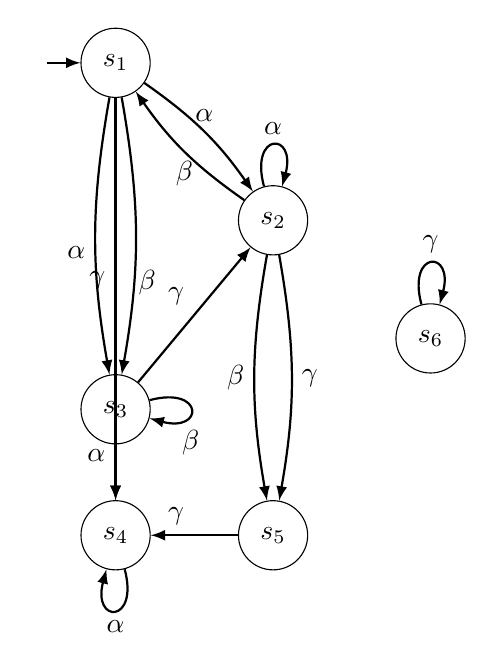
\begin{tikzpicture} [scale=2, every initial by arrow/.style={thick}]
		

		\path
		(\basex,		\basey) 		node[state,init] (s1) 	{$\state_1$} 
		(\basex+2,		\basey+0) 		node[state] (s2) 	{$\state_2$} 
		(\basex+1,		\basey-1.2) 	node[state] (s3) 	{$\state_3$} 
		(\basex,		\basey-2) 		node[state] (s4) 	{$\state_4$} 
		(\basex+2,		\basey-2) 		node[state] (s5) 	{$\state_5$}
		(\basex+3,		\basey-.75) 	node[state] (s6) 	{$\state_6$}
				
		;
		
%		
		\path [bendtrans] 	(s1) 	edge node [midway,above]				{\action} 		(s2);
		\path [bendtrans] 	(s1) 	edge node [near end,above right=-2pt]	{\actionb} 		(s3);
		\path [bendtransr] 	(s1) 	edge node [midway,below left]	{\action} 		(s3);
		\path [trans] 		(s1) 	edge node [midway,above left]	{\actionc} 		(s4);
		\path [bendtrans] 	(s2) 	edge node [midway,below]		{\actionb} 		(s1);
		\path [bendtransr] 	(s2) 	edge node [midway,left]			{\actionb} 		(s5);
		\path [bendtrans] 	(s2) 	edge node [midway,right]		{\actionc} 		(s5);
		\path [trans] 		(s3)	edge node [midway,above left]	{\actionc} 		(s2);
		\path [trans] 		(s3)	edge node [midway,above left]	{\action} 		(s4);
		\path [trans] 		(s5)	edge node [midway,above left]	{\actionc} 		(s4);
		
		\path [trans] 		(s2) 	edge [loop above] node [midway,above] {\action} 	(s2);
		\path [trans] 		(s3) 	edge [loop right] node [midway,below=4pt] {\actionb} 	(s3);
		\path [trans] 		(s4) 	edge [loop below] node [midway,below] {\action} 	(s4);
		\path [trans] 		(s6) 	edge [loop above] node [midway,above] {\actionc} 	(s6);
		
		
		%		midway, at start, near start, very near start, at end, near end, very near end
		
		
	\end{tikzpicture}
\end{document}
	\end{minipage}%
	\begin{minipage}{.5\textwidth}
		\hspace{5mm}
		\documentclass[tikz,preview]{standalone}
%\usepackage{prelude}

%%%%%%%%%%%%%%%%%%%%%%%%%%%%%%%%%%%% PACKAGES %%%%%%%%%%%%%%%%%%%%%%%%%%%%%%%%%%%%%%%%%%

\usepackage{inputenc,fontenc}
\usepackage[a4paper,margin=3cm]{geometry}
\usepackage[english]{babel}
%\usepackage[german]{babel}
%\usepackage[fixlanguage]{babelbib}


\usepackage{bbold}
\usepackage{amsthm}
\usepackage{amsmath}
\usepackage{amssymb} % doteqdot
\usepackage[dvipsnames]{xcolor}
\usepackage{standalone}
\usepackage{tikz}[mode=buildnew]
\usepackage{cite}
\usepackage{xspace}
\usepackage{relsize}
\usepackage{mathtools} % mathclap
%\usepackage{MnSymbol}
\usepackage{hyperref}
\usepackage{url}
\usepackage{listings} % for code
\usepackage[T1]{fontenc} %<
\hypersetup{
	colorlinks,
	citecolor=black,
	filecolor=black,
	linkcolor=black,
	urlcolor=black
}
\usepackage{pgfplots}
\pgfplotsset{compat=1.18}
%\usepackage{courier} %% Sets font for listing as Courier. But also for url and texttt!
\usepackage{listings, xcolor}
\usepackage{graphicx}
\usepackage{subcaption}

\usetikzlibrary{calc}
%\usepackage{xparse} % \newDocumentCommand for multiple optional arguments
%\usepackage{titlecaps}



%%%%%%%%%%%%%%%%%%%%%%%%%%%%%%%%%%%% THEOREMSTYLES %%%%%%%%%%%%%%%%%%%%%%%%%%%%%%%%%%

\theoremstyle{definition}
\newtheorem{definition}{Definition}[section]
\newtheorem{exmp}{Beispiel}[section]
%\AfterEndEnvironment{definition}{\noindent\ignorespaces}

\theoremstyle{theorem}
\newtheorem{theorem}{Satz}[section]
\newtheorem{proposition}{Proposition}[section]
%\AfterEndEnvironment{theorem}{\noindent\ignorespaces}

\theoremstyle{korollary}
\newtheorem{korollary}{Korollar}[section]
%\AfterEndEnvironment{korollary}{\noindent\ignorespaces}


\tikzset{
	mstate/.style={draw, circle, minimum size=.94cm}, 
	gstate/.style={draw, rectangle, minimum size=.8cm},
	varstate/.style={draw,rectangle, rounded corners, minimum size=1}, 
	trans/.style={draw, ->, thick},
	bendtrans/.style={draw, ->, thick, bend left=10},
	bendtransr/.style={draw, ->, thick, bend right=10},
	init/.style={initial, initial distance=6pt, initial text=},
	every loop/.style={min distance=5pt, looseness=8},
	>=latex
}
\usetikzlibrary{automata,positioning}

%auto shift/.style={auto=right,->,
%	to path={ let \p1=(\tikztostart),\p2=(\tikztotarget),
%		\n1={atan2(\y2-\y1,\x2-\x1)},\n2={\n1+180}
%		in ($(\tikztostart.{\n1})!1mm!270:(\tikztotarget.{\n2})$) -- 
%		($(\tikztotarget.{\n2})!1mm!90:(\tikztostart.{\n1})$) \tikztonodes}},

%%%%%%%%%%%%%%%%%%%%%%%%%%%%%%%%%%% MY MACROS %%%%%%%%%%%%%%%%%%%%%%%%%%%%%%%%%%%%%%%%%
%formatting
\newcommand{\comment}[2]{{\color{#1}#2}}
\newcommand{\redcomment}[1]{{\color{red}#1}}
\newcommand{\purpcomment}[1]{{\color{pink}#1}}
\newcommand{\bluecomment}[1]{{\color{blue}#1}}
\newcommand{\mt}[1]{\ensuremath{{#1}}\xspace}
\newcommand{\mynewcommand}[2]{\newcommand{#1}{\mt{#2}}} %% currently not used becaue of ide highlighting
\newcommand{\arr}{\mt{\to}}

%model checking terms
\newcommand{\mimicrel}{\mt{\mathcal{R}}}
\newcommand{\bisimeq}{\mt{\;\!\sim\;\!}}
\newcommand{\simorder}{\mt{\;\!\preceq\;\!}}
\newcommand{\simequiv}{\mt{\;\!\simeq\;\!}} %command already defined
\newcommand{\relts}{\mt{\;\!\bullet_{_{\tiny{TS}}}\;\!}}
\newcommand{\rel}{\mt{\;\!\bullet\;\!}}

%own names
\newcommand{\nm}[1]{#1\xspace}
\newcommand{\mdpN}{\nm{MDP}}
\newcommand{\mdpsN}{\nm{MDPs}}
\newcommand{\viewN}{\nm{view}}
\newcommand{\viewNC}{\nm{View}}
\newcommand{\viewsN}{\nm{views}}
\newcommand{\viewsNC}{\nm{Views}}
\newcommand{\grpfctsubN}{\nm{detached grouping function}}
\newcommand{\grpfctsubNC}{\nm{detached grouping function}}
\newcommand{\grpfctsubNCC}{\nm{Detached Grouping Function}}
\newcommand{\grpfctN}{\nm{grouping function}}
\newcommand{\grpfctNC}{\nm{Grouping function}}
\newcommand{\grpfctNCC}{\nm{Grouping Function}}
\newcommand{\grpfctsN}{\nm{grouping functions}}
\newcommand{\grpfctsNC}{\nm{Grouping functions}}
\newcommand{\grpfctsNCC}{\nm{Grouping Functions}}
\newcommand{\stmimicN}{\nm{state-mimic}}
\newcommand{\stmimicsN}{\nm{state-mimics}}
\newcommand{\stmimickingN}{\nm{state-mimicking}}
\newcommand{\stmimickedN}{\nm{state-mimicked}}
%\newcommand{\chosenphtypeNCC}{\nm{Transition System}}
%\newcommand{\chgphNC}{\nm{Transition system}}
%\newcommand{\chgphN}{\nm{transition system}}
%\newcommand{\chgphsNCC}{\nm{Transition Systems}}
%\newcommand{\chgphsNC}{\nm{Transition systems}}
%\newcommand{\chgphsN}{\nm{transition systems}}
\newcommand{\chgphNCC}{\nm{MDP}}
\newcommand{\chgphNC}{\nm{MDP}}
\newcommand{\chgphN}{\nm{MDP}}
\newcommand{\achgphN}{\nm{an MDP}}
\newcommand{\chgphsNCC}{\nm{MDPs}}
\newcommand{\chgphsNC}{\nm{MDPs}}
\newcommand{\chgphsN}{\nm{MDPs}}
\newcommand{\parllcompN}{\nm{parallel composition}}
\newcommand{\parllcompNC}{\nm{Parallel composition}}
\newcommand{\parllcompNCC}{\nm{Parallel Composition}}
\newcommand{\parllcompsN}{\nm{parallel compositions}}
\newcommand{\parllcompsNC}{\nm{Parallel compositions}}
\newcommand{\parllcompsNCC}{\nm{Parallel Compositions}}
\newcommand{\sccN}{\nm{SCC}}
\newcommand{\sccsN}{\nm{SCCs}}
\newcommand{\bsccN}{\nm{BSCC}}
\newcommand{\bsccsN}{\nm{BSCCs}}
\newcommand{\jgrapht}{\nm{jGraphtT}}

\newcommand{\outactident}{\nm{OutActionsIdent}}

%names
\newcommand{\iffN}{\nm{if and only if}}
\newcommand{\tsN}{\nm{TS}}

%% outactions identical
\newcommand{\outactidentstrong}{\nm{strong}}
\newcommand{\outactidentweak}{\nm{weak}}

% CORE DEFINITIONS
\newcommand{\grpfct}[1][\viewppty]{\mt{F_{#1}}}
\newcommand{\grpfctsub}[1][\viewppty]{\mt{\tilde{F}_{#1}}}
%\newcommand{\grpfctimg}[1]{\mt{{\grpfct}[{#1}]}}
%\newcommand{\fctimg}[2]{\mt{{#1}[{#2}]}}
\newcommand{\eqrelview}{\mt{R}}
\newcommand{\eqclassv}[1][\state]{\mt{\eqclass{#1}{\eqrelview}}}
\newcommand{\eqclasssetv}[1][\states]{\mt{{#1}/\eqrelview}} %OLD: \bigcup_{\state \in \states} \eqclassv
\newcommand{\viewid}{\mt{\mdp}}
\newcommand{\view}[1][\viewppty]{\mt{\viewid_{#1}}}
\newcommand{\imggrp}{\mt{\arbset}}
\newcommand{\imggrpsub}{\mt{X}}
\newcommand{\viewppty}{\mt{\theta}}
\newcommand{\pll}{\mt{\;\!\pllpure\;\!}}
\newcommand{\pllrev}{\mt{\pllpure^{-1}}}
\newcommand{\pllpure}{\mt{||}}
\newcommand{\compselectset}{\mt{Z}}
\newcommand{\compselectpure}{\mt{\pllpure_\compselectset}}
\newcommand{\compselect}{\mt{\;\pllpure_\compselectset\;}}
\newcommand{\remstates}{\mt{\bigcup_{\state \in \states \setminus \states_1}\{\{\state\}\}}}
\newcommand{\nogroupstates}[1][\states_2]{\mt{\bigcup_{\state \in \states \setminus {#1}}\{\{\state\}\}}}
\newcommand{\remelem}{\mt{\bullet}}
\newcommand{\nogroupset}{\mt{\xi}}
\newcommand{\remset}{\mt{\{\remelem\}}}
\newcommand{\gfctpll}{\mt{\grpfct[\pll]}}
\newcommand{\group}{\mt{\top}}
\newcommand{\imggrpbinview}{\mt{\{\remelem, \notppty\}}}
\newcommand{\viewappset}{\mt{\tilde{\states}}}
\newcommand{\hasppty}{\mt{\top}}
\newcommand{\notppty}{\mt{\bot}}
\newcommand{\disregardelem}{\mt{\Delta}}
\newcommand{\disregardelements}{\mt{{\disregardelem_1, \dots, \disregardelem_n}}}



%\newcommand{\mdp}{def}\mdp
%\newcommand{\mdpdef}



% EXAMPLE VIEWS
\newcommand{\pptyatomicprops}{\mt{\atomicprops}}
\newcommand{\pptyinitstates}{\mt{\initstates}}
\newcommand{\pptyinactsetsize}{\mt{|\inacts(\state)|}}
\newcommand{\pptyhasoutact}{\mt{\exists\outact}}
\newcommand{\pptyminoutact}[2]{\mt{#1\leq#2}}
\newcommand{\pptymaxoutact}[2]{\mt{#2\leq#1}}
\newcommand{\pptyspanoutact}[3]{\mt{#1\leq#2\leq#3}}
\newcommand{\pptyoutactsetsize}{\mt{|\outacts(\state)|}}
\newcommand{\pptyoutactsingle}{\mt{|\outacts(\state)|_1}}
\newcommand{\pptystrongoutactident}{\mt{\outacts(\state)_=}}
\newcommand{\pptyweakoutactident}{\mt{\outacts(\state)_\approx}}
\newcommand{\pptyhasinact}{\mt{\exists\inact}}
\newcommand{\pptymininact}[2]{\mt{#1\leq#2}}
\newcommand{\pptymaxinact}[2]{\mt{#2\leq#1}}
\newcommand{\pptyspaninact}[3]{\mt{#1\leq#2\leq#3}}
\newcommand{\pptyinactsingle}{\mt{|\inacts(\state)|_1}}
\newcommand{\pptystronginactident}{\mt{\inacts(\state)_=}}
\newcommand{\pptyweakinactident}{\mt{\inacts(\state)_\approx}}
\newcommand{\pptyparamvalueseq}{\mt{\var = \varval}}
\newcommand{\pptyparamvaluesneq}{\mt{\var \neq \varval}}
\newcommand{\pptyparamdnf}{\mt{VarDNF}}
\newcommand{\pptyparamcnf}{\mt{VarCNF}}
\newcommand{\pptyparamvalueseqopt}{\mt{\var = \varval}}
\newcommand{\pptyparamvalident}{\mt{Var:\varval}}
\newcommand{\pptydistance}{\mt{\distpath}}
\newcommand{\pptydistancerev}{\mt{\distpathrev}}
\newcommand{\pptydistancebi}{\mt{\distpathbi}}
\newcommand{\pptyhascycle}{\mt{\exists\cycle}}
\newcommand{\pptyexactactcycle}{\mt{\{\cycle_{\action,n}\}}}
\newcommand{\pptycycleset}{\mt{\cup{\{\state\}_\cycle}}}
\newcommand{\pptyexactcycle}{\mt{\{\cycle_n\}}}
\newcommand{\pptyscc}{\mt{scc}}
\newcommand{\pptybscc}{\mt{bscc}}
\newcommand{\pptyprop}{\mt{\redcomment{?}}}
\newcommand{\pptyident}{id}


\newcommand{\gfctatomicprops}{\mt{\grpfct[\pptyatomicprops]}}
\newcommand{\gfctinitstates}{\mt{\grpfct[\pptyinitstates]^\hasppty}}
\newcommand{\gfcthasoutaction}{\mt{\grpfct[\pptyhasoutact]^\hasppty}}
\newcommand{\gfctminoutaction}{\mt{\grpfct[\pptyminoutact{\numoutact}{\outact}]^\hasppty}}
\newcommand{\gfctmaxoutaction}{\mt{\grpfct[\pptymaxoutact{\numoutact}{\outact}]^\hasppty}}
\newcommand{\gfctspanoutaction}{\mt{\grpfct[\pptyspanoutact{\numoutactb}{\outact}{\numoutact}]^\hasppty}}
\newcommand{\gfctoutactsetsize}{\mt{\grpfct[\pptyoutactsetsize]}}
\newcommand{\gfctoutactsingle}{\mt{\grpfct[\pptyoutactsingle]^\notppty}}
\newcommand{\gfctstrongoutactident}{\mt{\grpfct[\pptystrongoutactident]}}
\newcommand{\gfctweakoutactident}{\mt{\grpfct[\pptyweakoutactident]}}
\newcommand{\gfcthasinaction}{\mt{\grpfct[\pptyhasinact]^\hasppty}}
\newcommand{\gfctmininaction}{\mt{\grpfct[\pptymininact{\numinact}{\inact}]^\hasppty}}
\newcommand{\gfctmaxinaction}{\mt{\grpfct[\pptymaxinact{\numinact}{\inact}]^\hasppty}}
\newcommand{\gfctspaninaction}{\mt{\grpfct[\pptyspaninact{\numinactb}{\inact}{\numinact}]^\hasppty}}
\newcommand{\gfctinactsetsize}{\mt{\grpfct[\pptyinactsetsize]}}
\newcommand{\gfctinactsingle}{\mt{\grpfct[\pptyinactsingle]^\notppty}}
\newcommand{\gfctstronginactident}{\mt{\grpfct[\pptystronginactident]}}
\newcommand{\gfctweakinactident}{\mt{\grpfct[\pptyweakinactident]}}
\newcommand{\gfctparamvalueseq}{\mt{\grpfct[\pptyparamvalueseq]^\hasppty}}
\newcommand{\gfctparamvaluesneq}{\mt{\grpfct[\pptyparamvaluesneq]^\hasppty}}
\newcommand{\gfctparamdnf}{\mt{\grpfct[\pptyparamdnf]^\hasppty}}
\newcommand{\gfctparamcnf}{\mt{\grpfct[\pptyparamcnf]^\hasppty}}
\newcommand{\gfctparamvalueseqopt}{\mt{\pptyparamvalueseqopt}}
\newcommand{\gfctparamvalident}{\mt{\grpfct[\pptyparamvalident]}}
\newcommand{\gfctdistance}{\mt{\grpfct[\pptydistance]}}
\newcommand{\gfctdistancerev}{\mt{\grpfct[\pptydistancerev]}}
\newcommand{\gfctdistancebi}{\mt{\grpfct[\pptydistancebi]}}
\newcommand{\gfcthascycle}{\mt{\grpfct[\pptyhascycle]}}
\newcommand{\gfctexactcycle}{\mt{\grpfct[\pptyexactcycle]}}
\newcommand{\gfctcycleset}{\mt{\grpfct[\pptycycleset]}}
\newcommand{\gfctexactactcycle}{\mt{\grpfct[\pptyexactactcycle]}}
\newcommand{\gfctscc}{\mt{\grpfct[\pptyscc]}}
\newcommand{\gfctbscc}{\mt{\grpfct[\pptybscc]}}
\newcommand{\gfctprop}{\mt{\grpfct[\pptyprop]}}
\newcommand{\gfctident}{\mt{\grpfct[\pptyident]}}

\newcommand{\gfctsubatomicprops}{\mt{\grpfctsub[\pptyatomicprops]}}
\newcommand{\gfctsubinitstates}{\mt{\grpfctsub[\pptyinitstates]^\hasppty}}
\newcommand{\gfctsubhasoutaction}{\mt{\grpfctsub[\pptyhasoutact]^\hasppty}}
\newcommand{\gfctsubminoutaction}{\mt{\grpfctsub[\pptyminoutact{\numoutact}{\outact}]^\hasppty}}
\newcommand{\gfctsubmaxoutaction}{\mt{\grpfctsub[\pptymaxoutact{\numoutact}{\outact}]^\hasppty}}
\newcommand{\gfctsubspanoutaction}{\mt{\grpfctsub[\pptyspanoutact{\numoutactb}{\outact}{\numoutact}]^\hasppty}}
\newcommand{\gfctsuboutactsetsize}{\mt{\grpfctsub[\pptyoutactsetsize]}}
\newcommand{\gfctsuboutactsingle}{\mt{\grpfctsub[\pptyoutactsingle]^\notppty}}
\newcommand{\gfctsubstrongoutactident}{\mt{\grpfctsub[\pptystrongoutactident]^\hasppty}}
\newcommand{\gfctsubweakoutactident}{\mt{\grpfctsub[\pptyweakoutactident]^\hasppty}}
\newcommand{\gfctsubhasinaction}{\mt{\grpfctsub[\pptyhasinact]}}
\newcommand{\gfctsubmininaction}{\mt{\grpfctsub[\pptymininact{\numinact}{\inact}]}}
\newcommand{\gfctsubmaxinaction}{\mt{\grpfctsub[\pptymaxinact{\numinact}{\inact}]}}
\newcommand{\gfctsubspaninaction}{\mt{\grpfctsub[\pptyspaninact{\numinactb}{\inact}{\numinact}]}}
\newcommand{\gfctsubinactsetsize}{\mt{\grpfctsub[\pptyinactsetsize]^\hasppty}}
\newcommand{\gfctsubinactsingle}{\mt{\grpfctsub[\pptyinactsingle]^\notppty}}
\newcommand{\gfctsubstronginactident}{\mt{\grpfctsub[\pptystronginactident]}}
\newcommand{\gfctsubweakinactident}{\mt{\grpfctsub[\pptyweakinactident]}}
\newcommand{\gfctsubparamvalueseq}{\mt{\grpfctsub[\pptyparamvalueseq]^\hasppty}}
\newcommand{\gfctsubparamvaluesneq}{\mt{\grpfctsub[\pptyparamvaluesneq]^\hasppty}}
\newcommand{\gfctsubparamdnf}{\mt{\grpfctsub[\pptyparamdnf]^\hasppty}}
\newcommand{\gfctsubparamcnf}{\mt{\grpfctsub[\pptyparamcnf]^\hasppty}}
\newcommand{\gfctsubparamvalueseqopt}{\mt{\pptyparamvalueseqopt}}
\newcommand{\gfctsubparamvalident}{\mt{\grpfctsub[\pptyparamvalident]}}
\newcommand{\gfctsubdistance}{\mt{\grpfctsub[\pptydistance]}}
\newcommand{\gfctsubdistancerev}{\mt{\grpfctsub[\pptydistancerev]}}
\newcommand{\gfctsubdistancebi}{\mt{\grpfctsub[\pptydistancebi]}}
\newcommand{\gfctsubhascycle}{\mt{\grpfctsub[\pptyhascycle]^\hasppty}}
\newcommand{\gfctsubexactcycle}{\mt{\grpfctsub[\pptyexactcycle]}}
\newcommand{\gfctsubcycleset}{\mt{\grpfctsub[\pptycycleset]}}
\newcommand{\gfctsubexactactcycle}{\mt{\grpfctsub[\pptyexactactcycle]}}
\newcommand{\gfctsubscc}{\mt{\grpfctsub[\pptyscc]}}
\newcommand{\gfctsubbscc}{\mt{\grpfctsub[\pptybscc]}}
\newcommand{\gfctsubprop}{\mt{\grpfctsub[\pptyprop]}}
\newcommand{\gfctsubident}{\mt{\grpfctsub[\pptyident]}}


\newcommand{\viewatomicprops}{\mt{\view[\pptyatomicprops]}}
\newcommand{\viewinitstates}{\mt{\view[\pptyinitstates]^\hasppty}}
\newcommand{\viewhasoutaction}{\mt{\view[\pptyhasoutact]^\hasppty}}
\newcommand{\viewminoutaction}{\mt{\view[\pptyminoutact{\numoutact}{\outact}]^\hasppty}}
\newcommand{\viewmaxoutaction}{\mt{\view[\pptymaxoutact{\numoutact}{\outact}]^\hasppty}}
\newcommand{\viewspanoutaction}{\mt{\view[\pptyspanoutact{\numoutactb}{\outact}{\numoutact}]^\hasppty}}
\newcommand{\viewoutactsetsize}{\mt{\view[\pptyoutactsetsize]}}
\newcommand{\viewoutactsingle}{\mt{\view[\pptyoutactsingle]^\notppty}}
\newcommand{\viewstrongoutactident}{\mt{\view[\pptystrongoutactident]}}
\newcommand{\viewweakoutactident}{\mt{\view[\pptyweakoutactident]}}
\newcommand{\viewhasinaction}{\mt{\view[\pptyhasinact]^\hasppty}}
\newcommand{\viewmininaction}{\mt{\view[\pptymininact{\numinact}{\inact}]^\hasppty}}
\newcommand{\viewmaxinaction}{\mt{\view[\pptymaxinact{\numinact}{\inact}]^\hasppty}}
\newcommand{\viewspaninaction}{\mt{\view[\pptyspaninact{\numinactb}{\inact}{\numinact}]^\hasppty}}
\newcommand{\viewinactsetsize}{\mt{\view[\pptyinactsetsize]}}
\newcommand{\viewinactsingle}{\mt{\view[\pptyinactsingle]^\notppty}}
\newcommand{\viewstronginactident}{\mt{\view[\pptystronginactident]}}
\newcommand{\viewweakinactident}{\mt{\view[\pptyweakinactident]}}
\newcommand{\viewparamvalueseq}{\mt{\view[\pptyparamvalueseq]}}
\newcommand{\viewparamvaluesneq}{\mt{\view[\pptyparamvaluesneq]}}
\newcommand{\viewparamdnf}{\mt{\view[\pptyparamdnf]^\hasppty}}
\newcommand{\viewparamcnf}{\mt{\view[\pptyparamcnf]^\hasppty}}
\newcommand{\viewparamvalueseqopt}{\mt{\pptyparamvalueseqopt}}
\newcommand{\viewparamvalident}{\mt{\view[\pptyparamvalident]}}
\newcommand{\viewdistance}{\mt{\view[\pptydistance]}}
\newcommand{\viewdistancerev}{\mt{\view[\pptydistancerev]}}
\newcommand{\viewdistancebi}{\mt{\view[\pptydistancebi]}}
\newcommand{\viewhascycle}{\mt{\view[\pptyhascycle]}}
\newcommand{\viewexactcycle}{\mt{\view[\pptyexactcycle]}}
\newcommand{\viewcycleset}{\mt{\view[\pptycycleset]}}
\newcommand{\viewexactactcycle}{\mt{\view[\pptyexactactcycle]}}
\newcommand{\viewscc}{\mt{\view[\pptyscc]}}
\newcommand{\viewbscc}{\mt{\view[\pptybscc]}}
\newcommand{\viewprop}{\mt{\view[\pptyprop]}}
\newcommand{\viewident}{\mt{\view[\pptyident]}}

%\newcommand{\viewatomicprops}{\mt{\view[\atomicprops]}}
%\newcommand{\viewinitstates}{\mt{\view[\initstates]}}
%\newcommand{\viewhasoutaction}{\mt{\view[\pptyhasoutact]}}
%\newcommand{\viewminoutaction}{\mt{\view[\pptyminoutact{\numoutact}{\outact}]}}
%\newcommand{\viewmaxoutaction}{\mt{\view[\pptymaxoutact{\numoutact}{\outact}]}}
%\newcommand{\viewspanoutaction}{\mt{\view[\pptyspanoutact{\numoutactb}{\outact}{\numoutact}]}}
%\newcommand{\viewoutactsetsize}{\mt{\view[\pptyoutactsetsize]}}
%\newcommand{\viewoutactsingle}{\mt{\view[\pptyoutactsingle]}}
%\newcommand{\viewstrongoutactident}{\mt{\view[\outacts(\state)_=]}}
%\newcommand{\viewweakoutactident}{\mt{\view[\outacts(\state)_\approx]}}
%\newcommand{\viewhasinaction}{\mt{\view[\pptyhasinact]}}
%\newcommand{\viewmininaction}{\mt{\view[\pptymininact{\numinact}{\inact}]}}
%\newcommand{\viewmaxinaction}{\mt{\view[\pptymaxinact{\numinact}{\inact}]}}
%\newcommand{\viewspaninaction}{\mt{\view[\pptyspaninact{\numinactb}{\inact}{\numinact}]}}
%\newcommand{\viewinactsetsize}{\mt{\view[\pptyinactsetsize]}}
%\newcommand{\viewinactsingle}{\mt{\view[\pptyinactsingle]}}
%\newcommand{\viewstronginactident}{\mt{\view[\inacts(\state)_=]}}
%\newcommand{\viewweakinactident}{\mt{\view[\inacts(\state)_\approx]}}
%\newcommand{\viewparamvalueseq}{\mt{\view[\var = \varval]}}
%\newcommand{\viewparamvaluesneq}{\mt{\view[\var \neq \varval]}}
%\newcommand{\viewparamdnf}{\mt{\view[VarDNF]}}
%\newcommand{\viewparamcnf}{\mt{\view[VarCNF]}}
%\newcommand{\viewparamvalident}{\mt{\view[\pptyparamvalident]}}
%\newcommand{\viewdistance}{\mt{\view[\pptydistance]}}
%\newcommand{\viewhascycle}{\mt{\view[\exists\cycle]}}
%\newcommand{\viewexactcycle}{\mt{\view[\pptyexactcycle]}}
%\newcommand{\viewcycleset}{\mt{\view[\pptycycleset]}}
%\newcommand{\viewexactactcycle}{\mt{\view[\pptyexactactcycle]}}
%\newcommand{\viewscc}{\mt{\view[scc]}}
%\newcommand{\viewbscc}{\mt{\view[bscc]}}

%actions
\newcommand{\numoutact}{\mt{n}}
\newcommand{\numoutactb}{\mt{m}}
\newcommand{\numinact}{\mt{n}}
\newcommand{\numinactb}{\mt{m}}

\newcommand{\predmaxoutact}[1][\numoutact]{\mt{Q_{\outact\leq#1}(\state,\state_1, \dots, \state_{#1+1})}}
\newcommand{\predminoutact}[1][\numoutact]{\mt{Q_{#1\leq\outact}(\state,\state_1, \dots, \state_{#1})}}
\newcommand{\formoutact}[1][\state]{\mt{C_{#1,\outact}}}
\newcommand{\predmaxinact}[1][\numinact]{\mt{Q_{\inact\leq#1}(\state,\state_1, \dots, \state_{#1+1})}}
\newcommand{\predmininact}[1][\numinact]{\mt{Q_{#1\leq\inact}(\state,\state_1, \dots, \state_{#1})}}

\newcommand{\outact}[1][\action]{\mt{\overrightarrow{#1}}}
\newcommand{\outacts}{\mt{\overrightarrow{\actions}}}
\newcommand{\inact}{\mt{\overleftarrow{\action}}}
\newcommand{\inacts}[1][\action]{\mt{\overleftarrow{#1}}}

%%Parameters
\newcommand{\vars}[1][\mdp]{\mt{V\!ar_{#1}}}
\newcommand{\var}{\mt{x}}
\newcommand{\varstate}[1][]{\mt{\var_{\state#1}}}
\newcommand{\varval}{\mt{a}}
\newcommand{\vareval}[1][\mdp]{\mt{V\!arEval_{#1}}}
\newcommand{\varevalimg}[1][\mdp]{\mt{\vareval[#1][\states,\vars]}}
\newcommand{\varevalimgset}{\mt{\arbset}}
\newcommand{\someparam}{\mt{\tilde{x}}}
\newcommand{\eqorneq}{\mt{\;\doteqdot\;}}
\newcommand{\varstyle}[2]{\mt{\langle#1,#2\rangle}}




%\makeatletter
%\newcommand{\overleftrightsmallarrow}{\mathpalette{\overarrowsmall@\leftrightarrowfill@}}
%\newcommand{\overrightsmallarrow}{\mathpalette{\overarrowsmall@\rightarrowfill@}}
%\newcommand{\overleftsmallarrow}{\mathpalette{\overarrowsmall@\leftarrowfill@}}
%\newcommand{\overarrowsmall@}[3]{%
%	\vbox{%
%		\ialign{%
%			##\crcr
%			#1{\smaller@style{#2}}\crcr
%			\noalign{\nointerlineskip}%
%			$\m@th\hfil#2#3\hfil$\crcr
%		}%
%	}%
%}
%\def\smaller@style#1{%
%	\ifx#1\displaystyle\scriptstyle\else
%	\ifx#1\textstyle\scriptstyle\else
%	\scriptscriptstyle
%	\fi
%	\fi
%}
%\makeatother
%\newcommand{\te}[1]{\overleftrightsmallarrow{#1}}

% Distance
\newcommand{\fctdist}{\mt{distance}}
\newcommand{\fctdistdefault}{\mt{\fctdist(\chgph, \smstates, \grandist)}}
\newcommand{\distval}{\mt{d}}
\newcommand{\grandist}{\mt{n}}
\let\path\oldpath
\newcommand{\path}{\mt{P}}
\newcommand{\pathbi}{\mt{\bar{\path}}}
\newcommand{\pathsecfull}{\mt{(\state_0, \action_0, \state_1, \action_1, \dots, \action_{n}, \state_{n+1})}}
\newcommand{\lenpath}{\mt{len}}
\newcommand{\pfirst}{\mt{first}}
\newcommand{\plast}{\mt{last}}
\newcommand{\pathset}{\mt{\path_\chgph}}
\newcommand{\pathbiset}{\mt{\pathbi_\chgph}}
\newcommand{\distpath}{\mt{\overrightarrow{dist}}}
\newcommand{\distpathrev}{\mt{\overleftarrow{dist}}}
\newcommand{\distpathbi}{\mt{\overline{dist}}}
%Cycles
\newcommand{\cyclesecfull}{\mt{(\state_0, \action_0, \state_1, \action_1, \dots, \action_{n-1}, \state_0)}}
\newcommand{\fctfindcycles}{\mt{findCycles}}
\newcommand{\cycle}{\mt{C}}
\newcommand{\cycleset}{\mt{\cycle_{\mdp, n}}}
\newcommand{\lencycle}{\mt{len}}
% strongly connected components
\newcommand{\scc}{\mt{T}}
\newcommand{\setscc}{\mt{SCC_{\chgph,n}}}
\newcommand{\setbscc}{\mt{BSCC_{\chgph,n}}}

% properties
\newcommand{\propfct}{\mt{f}}

% all Systems
\newcommand{\chgph}{\mt{\mdp}}
\newcommand{\chgphtuple}{\mt{\mdptuple}}
\newcommand{\chgphtupledist}{\mt{\mdptupledist}}

\newcommand{\states}{\mt{S}}
\newcommand{\actions}{\mt{Act}}
\newcommand{\atomicprops}{\mt{AP}}
\newcommand{\labelingfct}{\mt{L}}
\newcommand{\init}{\mt{\initdistrib}} % use MDP % refers to the underlying set
\newcommand{\trans}{\mt{\probtfunc}} % use MDP % refers to the underlying set
\newcommand{\smstates}{\mt{\tilde{\states}}}


\newcommand{\state}{\mt{s}}
\newcommand{\action}{\mt{\alpha}}
\newcommand{\actionb}{\mt{\beta}}
\newcommand{\actionc}{\mt{\gamma}}
\newcommand{\smstate}{\mt{\tilde{\state}}}



% transition sysstems
\newcommand{\ts}{\mt{TS}}
\newcommand{\transitionrel}{\mt{\longrightarrow}}
\newcommand{\initstates}{\mt{I}}
\newcommand{\transitionsystem}{\mt
	{(\states, \actions, \transitionrel, \initstates, \atomicprops, \labelingfct)}
}
\newcommand{\tstupledist}{\mt{(\states', \actions',\transitionrel', \initstates', \labelingfct')}}


%Markov chains and MDP
\newcommand{\mdp}{\mt{\autm}}
\newcommand{\mdptuple}{\mt{(\states, \actions, \probtfunc, \initdistrib, \atomicprops, \labelingfct)}}
\newcommand{\mdptupledist}{\mt{(\states', \actions', \probtfunc', \initdistrib', \atomicprops', \labelingfct')}}
\newcommand{\autm}{\mt{\mathcal{M}}}
\newcommand{\probtfunc}{\mt{\textbf{P}}}
\newcommand{\initdistrib}{\mt{\iota_{init}}}


%maths
\newcommand{\powerset}[1]{\mt{\mathcal{P}(#1)}}
\newcommand{\eqclass}[2]{\mt{[#1]_{#2}}}%{\mt{#1 / #2}}
\newcommand{\impr}{\mt{\hspace{3mm}\Rightarrow\hspace{2mm}}}
\newcommand{\impl}{\mt{\hspace{3mm}\Leftarrow\hspace{2mm}}}
\newcommand{\natnums}{\mt{\mathbb{N}}} 
\newcommand{\realnums}{\mt{\mathbb{R}}}
\newcommand{\intmodn}[1][n]{\mt{\mathbb{Z}_{#1}}}
\newcommand{\arbset}{\mt{M}}
\newcommand{\bigsum}[2][]{\mt{\mathlarger{\sum}_{#2}^{#1}}}
\newcommand{\bbigsum}[2][]{\mt{\mathlarger{\mathlarger{\sum}}_{#2}^{#1}}}
\newcommand{\invimage}[2]{#1^{\mt{-1}(#2)}}
\newcommand{\img}{\mt{Img}}
\newcommand{\cond}{\mt{\,|\,}}

%tickz
%% \definecolor{darkred}{RGB}{196, 42, 42}

%implementation
\newcommand{\pmcvis}{\nm{PMC-Vis}}





\begin{document}
	\newcommand{\basex}{0}
	\newcommand{\basey}{0}
	\newcommand{\createstate}[3]{\node[draw, circle, minimum size=1cm] (#1) at (#2) {#3}}
	
	
	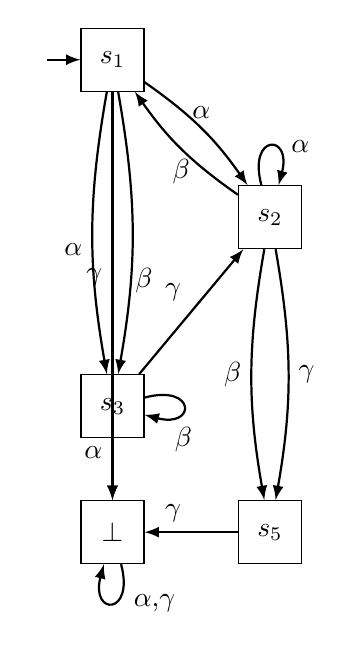
\begin{tikzpicture} [scale=2, every initial by arrow/.style={thick}]
		
		
		\path
		(\basex,		\basey) 		node[gstate,init] (s1) 	{$\state_1$} 
		(\basex+2,		\basey+0) 		node[gstate] (s2) 	{$\state_2$} 
		(\basex+1,		\basey-1.2) 	node[gstate] (s3) 	{$\state_3$} 
		(\basex,		\basey-2) 		node[gstate] (sbot) 	{$\notppty$} 
		(\basex+2,		\basey-2) 		node[gstate] (s5) 	{$\state_5$}
		
		;
		
		%		
		\path [bendtrans] 	(s1) 	edge node [midway,above]				{\action} 		(s2);
		\path [bendtrans] 	(s1) 	edge node [near end,above right=-2pt]	{\actionb} 		(s3);
		\path [bendtransr] 	(s1) 	edge node [midway,below left]	{\action} 		(s3);
		\path [trans] 		(s1) 	edge node [midway,above left]	{\actionc} 		(sbot);
		\path [bendtrans] 	(s2) 	edge node [midway,below]		{\actionb} 		(s1);
		\path [bendtransr] 	(s2) 	edge node [midway,left]			{\actionb} 		(s5);
		\path [bendtrans] 	(s2) 	edge node [midway,right]		{\actionc} 		(s5);
		\path [trans] 		(s3)	edge node [midway,above left]	{\actionc} 		(s2);
		\path [trans] 		(s3)	edge node [midway,above left]	{\action} 		(sbot);
		\path [trans] 		(s5)	edge node [midway,above left]	{\actionc} 		(sbot);
		
		\path [trans] 		(s2) 	edge [loop above] node [midway,right=4pt] {\action} 	(s2);
		\path [trans] 		(s3) 	edge [loop right] node [midway,below=4pt] {\actionb} 	(s3);
		\path [trans] 		(sbot) 	edge [loop below] node [midway,right=4pt] {\action,\actionc} 	(sbot);
		
		
		%		midway, at start, near start, very near start, at end, near end, very near end
		
		
	\end{tikzpicture}
\end{document}
	\end{minipage}
	\caption{Simplified representations of \mdp (left) and the \viewN \viewhasoutaction on it (right)}
	\label{fig:outActHasAfter}  
\end{figure}





Since actions are a very important part of \chgphsN as well as of its more powerful siblings MDPs and MCs it seems useful to further enhance this view and look at variants of it. Instead of only grouping states that only \emph{have} outgoing actions we could also quantify the amount of times that action should be outgoing.



For example we could require that a given action has to be outgoing a minimum amount of times. 

\begin{definition}
	Let $\chgph = \chgphtuple$ be \achgphN and $\action \in \actions$. The view \viewminoutaction is defined by its \grpfctN $\gfctminoutaction : \states \to \arbset$ with
	
	\[
	\state \mapsto
	\begin{cases}
			\group,				& \text{if } \exists \state_1, \dots, \state_\numoutact \in \states:  \predminoutact\\
			\remelem,          	& \text{otherwise}
		\end{cases}
	\]
	
	where $\imggrp := \imggrpbinview$,
	%	\actions \cup \remset$
	 $\numoutact \in \natnums$ is the minimum amount of times a transition with action \action has to be outgoing in order to be grouped with the other states and
	\[
	\predminoutact := ((\state, \action, \state_1), \dots, (\state, \action, \state_\numoutact) \in \trans) \land |\{\state_1, \dots, \state_\numoutact\}| = \numoutact
	\]
	
	is a first order logic predicate.
	\label{def:minoutaction}
\end{definition}

The number  and  
The predicate \predminoutact requires that there are transitions with action \action to \numoutact distinct states.

For $\state_1,\state_2 \in \states$ it is $\gfctminoutaction(\state_1) = \gfctminoutaction(\state_2)$ \iffN there exist distinct $\state_{a_1}, \dots, \state_{a_\numoutact} \in \states$ and distinct $\state_{b_1}, \dots, \state_{b_\numoutact} \in \states$ so that $(\state_1, \action, \state_{a_1}), \dots, (\state_1, \action, \state_{a_\numoutact}) \in \trans$ and $(\state_2, \action, \state_{b_1}), \dots, (\state_2, \action, \state_{b_\numoutact}) \in \trans$ or $\state_1 = \state_2$. According to Definition \ref{def:eqrelview} it is 
\begin{align*}
	\eqclassv &= \{\state \in \states \mid \gfctminoutaction(\state) = \action\} &\text{if } \predminoutact \\ 
	\eqclassv &= \{\state \in \states \mid \gfctminoutaction(\state) = \state\} = \{\state\} &\text{ otherwise}
\end{align*}

By this we obtain the \viewN $\viewminoutaction$ for a given \chgphN \chgph where $\states' = \bigcup_{\state \in \states} \{\eqclassv\} =: \states_1 \cup \states_2$ where 

\begin{align*}
	\states_1 &:= \{\state \in \states \mid \exists \state_1, \dots, \state_\numoutact \in \states: \predminoutact\} \\ %(\state, \action, \state_1), \dots, (\state, \action, \state_\numoutact) \in \trans, |\{\state_1, \dots, \state_\numoutact\}| = \numoutact\} \\ 
	&\hspace{1.15mm}= \{\state \in \states \mid \text{the action } \action \text{ is outgoing at least } \numoutact \text{ times} \} \text{ and} \\
	\states_2 &:= \remstates.	
\end{align*}

In a similar fashion we define view that groups states where at most a certain number of times a given action is outgoing. 

\begin{definition}
	Let $\chgph = \chgphtuple$ be \achgphN and $\action \in \actions$. The view \viewmaxoutaction is defined by its \grpfctN $\gfctmaxoutaction : \states \to \arbset$ with
	
	\[
	\state \mapsto
	\begin{cases}
			\group,				& \text{if } \forall \state_1, \dots, \state_{\numoutact+1} \in \states: \predmaxoutact \\
			\remelem,          	& \text{otherwise}
		\end{cases}
	\]
	
	where $\imggrp := \imggrpbinview$,
%	$\numoutact \in \natnums$ 
	is the maximal number of times a transition with action \action may be outgoing and 
	\[
	\predmaxoutact := ((\state, \action, \state_1), \dots, (\state, \action, \state_{\numoutact+1}) \in \trans) \implies \bigvee_{\mathclap{\substack{i,j \in \{1,\dots, \numoutact+1\} \\ i < j}}} \state_i = \state_j
	\]
	is a first order logic predicate.
	\label{def:viewmaxoutaction}
\end{definition}

It ensures that if there are one more than \numoutact outgoing transitions with an action \action at least two of the states where the transitions \redcomment{end} are in fact the same. Since this is required for all possible combinations of $\numoutact + 1$ states by the grouping function, only states that have at most \numoutact outgoing actions will be assigned with \action by the grouping function. The reasoning about the equality of the \grpfctN values, the obtained equivalence classes and the resulting set of states $\states'$ of the view is analogous to \viewminoutaction.

\begin{figure}[h]
	\begin{minipage}{.5\textwidth}
		\hspace{5mm}
		\documentclass[tikz,preview]{standalone}
%\usepackage{prelude}

%%%%%%%%%%%%%%%%%%%%%%%%%%%%%%%%%%%% PACKAGES %%%%%%%%%%%%%%%%%%%%%%%%%%%%%%%%%%%%%%%%%%

\usepackage{inputenc,fontenc}
\usepackage[a4paper,margin=3cm]{geometry}
\usepackage[english]{babel}
%\usepackage[german]{babel}
%\usepackage[fixlanguage]{babelbib}


\usepackage{bbold}
\usepackage{amsthm}
\usepackage{amsmath}
\usepackage{amssymb} % doteqdot
\usepackage[dvipsnames]{xcolor}
\usepackage{standalone}
\usepackage{tikz}[mode=buildnew]
\usepackage{cite}
\usepackage{xspace}
\usepackage{relsize}
\usepackage{mathtools} % mathclap
%\usepackage{MnSymbol}
\usepackage{hyperref}
\usepackage{url}
\usepackage{listings} % for code
\usepackage[T1]{fontenc} %<
\hypersetup{
	colorlinks,
	citecolor=black,
	filecolor=black,
	linkcolor=black,
	urlcolor=black
}
\usepackage{pgfplots}
\pgfplotsset{compat=1.18}
%\usepackage{courier} %% Sets font for listing as Courier. But also for url and texttt!
\usepackage{listings, xcolor}
\usepackage{graphicx}
\usepackage{subcaption}

\usetikzlibrary{calc}
%\usepackage{xparse} % \newDocumentCommand for multiple optional arguments
%\usepackage{titlecaps}



%%%%%%%%%%%%%%%%%%%%%%%%%%%%%%%%%%%% THEOREMSTYLES %%%%%%%%%%%%%%%%%%%%%%%%%%%%%%%%%%

\theoremstyle{definition}
\newtheorem{definition}{Definition}[section]
\newtheorem{exmp}{Beispiel}[section]
%\AfterEndEnvironment{definition}{\noindent\ignorespaces}

\theoremstyle{theorem}
\newtheorem{theorem}{Satz}[section]
\newtheorem{proposition}{Proposition}[section]
%\AfterEndEnvironment{theorem}{\noindent\ignorespaces}

\theoremstyle{korollary}
\newtheorem{korollary}{Korollar}[section]
%\AfterEndEnvironment{korollary}{\noindent\ignorespaces}


\tikzset{
	mstate/.style={draw, circle, minimum size=.94cm}, 
	gstate/.style={draw, rectangle, minimum size=.8cm},
	varstate/.style={draw,rectangle, rounded corners, minimum size=1}, 
	trans/.style={draw, ->, thick},
	bendtrans/.style={draw, ->, thick, bend left=10},
	bendtransr/.style={draw, ->, thick, bend right=10},
	init/.style={initial, initial distance=6pt, initial text=},
	every loop/.style={min distance=5pt, looseness=8},
	>=latex
}
\usetikzlibrary{automata,positioning}

%auto shift/.style={auto=right,->,
%	to path={ let \p1=(\tikztostart),\p2=(\tikztotarget),
%		\n1={atan2(\y2-\y1,\x2-\x1)},\n2={\n1+180}
%		in ($(\tikztostart.{\n1})!1mm!270:(\tikztotarget.{\n2})$) -- 
%		($(\tikztotarget.{\n2})!1mm!90:(\tikztostart.{\n1})$) \tikztonodes}},

%%%%%%%%%%%%%%%%%%%%%%%%%%%%%%%%%%% MY MACROS %%%%%%%%%%%%%%%%%%%%%%%%%%%%%%%%%%%%%%%%%
%formatting
\newcommand{\comment}[2]{{\color{#1}#2}}
\newcommand{\redcomment}[1]{{\color{red}#1}}
\newcommand{\purpcomment}[1]{{\color{pink}#1}}
\newcommand{\bluecomment}[1]{{\color{blue}#1}}
\newcommand{\mt}[1]{\ensuremath{{#1}}\xspace}
\newcommand{\mynewcommand}[2]{\newcommand{#1}{\mt{#2}}} %% currently not used becaue of ide highlighting
\newcommand{\arr}{\mt{\to}}

%model checking terms
\newcommand{\mimicrel}{\mt{\mathcal{R}}}
\newcommand{\bisimeq}{\mt{\;\!\sim\;\!}}
\newcommand{\simorder}{\mt{\;\!\preceq\;\!}}
\newcommand{\simequiv}{\mt{\;\!\simeq\;\!}} %command already defined
\newcommand{\relts}{\mt{\;\!\bullet_{_{\tiny{TS}}}\;\!}}
\newcommand{\rel}{\mt{\;\!\bullet\;\!}}

%own names
\newcommand{\nm}[1]{#1\xspace}
\newcommand{\mdpN}{\nm{MDP}}
\newcommand{\mdpsN}{\nm{MDPs}}
\newcommand{\viewN}{\nm{view}}
\newcommand{\viewNC}{\nm{View}}
\newcommand{\viewsN}{\nm{views}}
\newcommand{\viewsNC}{\nm{Views}}
\newcommand{\grpfctsubN}{\nm{detached grouping function}}
\newcommand{\grpfctsubNC}{\nm{detached grouping function}}
\newcommand{\grpfctsubNCC}{\nm{Detached Grouping Function}}
\newcommand{\grpfctN}{\nm{grouping function}}
\newcommand{\grpfctNC}{\nm{Grouping function}}
\newcommand{\grpfctNCC}{\nm{Grouping Function}}
\newcommand{\grpfctsN}{\nm{grouping functions}}
\newcommand{\grpfctsNC}{\nm{Grouping functions}}
\newcommand{\grpfctsNCC}{\nm{Grouping Functions}}
\newcommand{\stmimicN}{\nm{state-mimic}}
\newcommand{\stmimicsN}{\nm{state-mimics}}
\newcommand{\stmimickingN}{\nm{state-mimicking}}
\newcommand{\stmimickedN}{\nm{state-mimicked}}
%\newcommand{\chosenphtypeNCC}{\nm{Transition System}}
%\newcommand{\chgphNC}{\nm{Transition system}}
%\newcommand{\chgphN}{\nm{transition system}}
%\newcommand{\chgphsNCC}{\nm{Transition Systems}}
%\newcommand{\chgphsNC}{\nm{Transition systems}}
%\newcommand{\chgphsN}{\nm{transition systems}}
\newcommand{\chgphNCC}{\nm{MDP}}
\newcommand{\chgphNC}{\nm{MDP}}
\newcommand{\chgphN}{\nm{MDP}}
\newcommand{\achgphN}{\nm{an MDP}}
\newcommand{\chgphsNCC}{\nm{MDPs}}
\newcommand{\chgphsNC}{\nm{MDPs}}
\newcommand{\chgphsN}{\nm{MDPs}}
\newcommand{\parllcompN}{\nm{parallel composition}}
\newcommand{\parllcompNC}{\nm{Parallel composition}}
\newcommand{\parllcompNCC}{\nm{Parallel Composition}}
\newcommand{\parllcompsN}{\nm{parallel compositions}}
\newcommand{\parllcompsNC}{\nm{Parallel compositions}}
\newcommand{\parllcompsNCC}{\nm{Parallel Compositions}}
\newcommand{\sccN}{\nm{SCC}}
\newcommand{\sccsN}{\nm{SCCs}}
\newcommand{\bsccN}{\nm{BSCC}}
\newcommand{\bsccsN}{\nm{BSCCs}}
\newcommand{\jgrapht}{\nm{jGraphtT}}

\newcommand{\outactident}{\nm{OutActionsIdent}}

%names
\newcommand{\iffN}{\nm{if and only if}}
\newcommand{\tsN}{\nm{TS}}

%% outactions identical
\newcommand{\outactidentstrong}{\nm{strong}}
\newcommand{\outactidentweak}{\nm{weak}}

% CORE DEFINITIONS
\newcommand{\grpfct}[1][\viewppty]{\mt{F_{#1}}}
\newcommand{\grpfctsub}[1][\viewppty]{\mt{\tilde{F}_{#1}}}
%\newcommand{\grpfctimg}[1]{\mt{{\grpfct}[{#1}]}}
%\newcommand{\fctimg}[2]{\mt{{#1}[{#2}]}}
\newcommand{\eqrelview}{\mt{R}}
\newcommand{\eqclassv}[1][\state]{\mt{\eqclass{#1}{\eqrelview}}}
\newcommand{\eqclasssetv}[1][\states]{\mt{{#1}/\eqrelview}} %OLD: \bigcup_{\state \in \states} \eqclassv
\newcommand{\viewid}{\mt{\mdp}}
\newcommand{\view}[1][\viewppty]{\mt{\viewid_{#1}}}
\newcommand{\imggrp}{\mt{\arbset}}
\newcommand{\imggrpsub}{\mt{X}}
\newcommand{\viewppty}{\mt{\theta}}
\newcommand{\pll}{\mt{\;\!\pllpure\;\!}}
\newcommand{\pllrev}{\mt{\pllpure^{-1}}}
\newcommand{\pllpure}{\mt{||}}
\newcommand{\compselectset}{\mt{Z}}
\newcommand{\compselectpure}{\mt{\pllpure_\compselectset}}
\newcommand{\compselect}{\mt{\;\pllpure_\compselectset\;}}
\newcommand{\remstates}{\mt{\bigcup_{\state \in \states \setminus \states_1}\{\{\state\}\}}}
\newcommand{\nogroupstates}[1][\states_2]{\mt{\bigcup_{\state \in \states \setminus {#1}}\{\{\state\}\}}}
\newcommand{\remelem}{\mt{\bullet}}
\newcommand{\nogroupset}{\mt{\xi}}
\newcommand{\remset}{\mt{\{\remelem\}}}
\newcommand{\gfctpll}{\mt{\grpfct[\pll]}}
\newcommand{\group}{\mt{\top}}
\newcommand{\imggrpbinview}{\mt{\{\remelem, \notppty\}}}
\newcommand{\viewappset}{\mt{\tilde{\states}}}
\newcommand{\hasppty}{\mt{\top}}
\newcommand{\notppty}{\mt{\bot}}
\newcommand{\disregardelem}{\mt{\Delta}}
\newcommand{\disregardelements}{\mt{{\disregardelem_1, \dots, \disregardelem_n}}}



%\newcommand{\mdp}{def}\mdp
%\newcommand{\mdpdef}



% EXAMPLE VIEWS
\newcommand{\pptyatomicprops}{\mt{\atomicprops}}
\newcommand{\pptyinitstates}{\mt{\initstates}}
\newcommand{\pptyinactsetsize}{\mt{|\inacts(\state)|}}
\newcommand{\pptyhasoutact}{\mt{\exists\outact}}
\newcommand{\pptyminoutact}[2]{\mt{#1\leq#2}}
\newcommand{\pptymaxoutact}[2]{\mt{#2\leq#1}}
\newcommand{\pptyspanoutact}[3]{\mt{#1\leq#2\leq#3}}
\newcommand{\pptyoutactsetsize}{\mt{|\outacts(\state)|}}
\newcommand{\pptyoutactsingle}{\mt{|\outacts(\state)|_1}}
\newcommand{\pptystrongoutactident}{\mt{\outacts(\state)_=}}
\newcommand{\pptyweakoutactident}{\mt{\outacts(\state)_\approx}}
\newcommand{\pptyhasinact}{\mt{\exists\inact}}
\newcommand{\pptymininact}[2]{\mt{#1\leq#2}}
\newcommand{\pptymaxinact}[2]{\mt{#2\leq#1}}
\newcommand{\pptyspaninact}[3]{\mt{#1\leq#2\leq#3}}
\newcommand{\pptyinactsingle}{\mt{|\inacts(\state)|_1}}
\newcommand{\pptystronginactident}{\mt{\inacts(\state)_=}}
\newcommand{\pptyweakinactident}{\mt{\inacts(\state)_\approx}}
\newcommand{\pptyparamvalueseq}{\mt{\var = \varval}}
\newcommand{\pptyparamvaluesneq}{\mt{\var \neq \varval}}
\newcommand{\pptyparamdnf}{\mt{VarDNF}}
\newcommand{\pptyparamcnf}{\mt{VarCNF}}
\newcommand{\pptyparamvalueseqopt}{\mt{\var = \varval}}
\newcommand{\pptyparamvalident}{\mt{Var:\varval}}
\newcommand{\pptydistance}{\mt{\distpath}}
\newcommand{\pptydistancerev}{\mt{\distpathrev}}
\newcommand{\pptydistancebi}{\mt{\distpathbi}}
\newcommand{\pptyhascycle}{\mt{\exists\cycle}}
\newcommand{\pptyexactactcycle}{\mt{\{\cycle_{\action,n}\}}}
\newcommand{\pptycycleset}{\mt{\cup{\{\state\}_\cycle}}}
\newcommand{\pptyexactcycle}{\mt{\{\cycle_n\}}}
\newcommand{\pptyscc}{\mt{scc}}
\newcommand{\pptybscc}{\mt{bscc}}
\newcommand{\pptyprop}{\mt{\redcomment{?}}}
\newcommand{\pptyident}{id}


\newcommand{\gfctatomicprops}{\mt{\grpfct[\pptyatomicprops]}}
\newcommand{\gfctinitstates}{\mt{\grpfct[\pptyinitstates]^\hasppty}}
\newcommand{\gfcthasoutaction}{\mt{\grpfct[\pptyhasoutact]^\hasppty}}
\newcommand{\gfctminoutaction}{\mt{\grpfct[\pptyminoutact{\numoutact}{\outact}]^\hasppty}}
\newcommand{\gfctmaxoutaction}{\mt{\grpfct[\pptymaxoutact{\numoutact}{\outact}]^\hasppty}}
\newcommand{\gfctspanoutaction}{\mt{\grpfct[\pptyspanoutact{\numoutactb}{\outact}{\numoutact}]^\hasppty}}
\newcommand{\gfctoutactsetsize}{\mt{\grpfct[\pptyoutactsetsize]}}
\newcommand{\gfctoutactsingle}{\mt{\grpfct[\pptyoutactsingle]^\notppty}}
\newcommand{\gfctstrongoutactident}{\mt{\grpfct[\pptystrongoutactident]}}
\newcommand{\gfctweakoutactident}{\mt{\grpfct[\pptyweakoutactident]}}
\newcommand{\gfcthasinaction}{\mt{\grpfct[\pptyhasinact]^\hasppty}}
\newcommand{\gfctmininaction}{\mt{\grpfct[\pptymininact{\numinact}{\inact}]^\hasppty}}
\newcommand{\gfctmaxinaction}{\mt{\grpfct[\pptymaxinact{\numinact}{\inact}]^\hasppty}}
\newcommand{\gfctspaninaction}{\mt{\grpfct[\pptyspaninact{\numinactb}{\inact}{\numinact}]^\hasppty}}
\newcommand{\gfctinactsetsize}{\mt{\grpfct[\pptyinactsetsize]}}
\newcommand{\gfctinactsingle}{\mt{\grpfct[\pptyinactsingle]^\notppty}}
\newcommand{\gfctstronginactident}{\mt{\grpfct[\pptystronginactident]}}
\newcommand{\gfctweakinactident}{\mt{\grpfct[\pptyweakinactident]}}
\newcommand{\gfctparamvalueseq}{\mt{\grpfct[\pptyparamvalueseq]^\hasppty}}
\newcommand{\gfctparamvaluesneq}{\mt{\grpfct[\pptyparamvaluesneq]^\hasppty}}
\newcommand{\gfctparamdnf}{\mt{\grpfct[\pptyparamdnf]^\hasppty}}
\newcommand{\gfctparamcnf}{\mt{\grpfct[\pptyparamcnf]^\hasppty}}
\newcommand{\gfctparamvalueseqopt}{\mt{\pptyparamvalueseqopt}}
\newcommand{\gfctparamvalident}{\mt{\grpfct[\pptyparamvalident]}}
\newcommand{\gfctdistance}{\mt{\grpfct[\pptydistance]}}
\newcommand{\gfctdistancerev}{\mt{\grpfct[\pptydistancerev]}}
\newcommand{\gfctdistancebi}{\mt{\grpfct[\pptydistancebi]}}
\newcommand{\gfcthascycle}{\mt{\grpfct[\pptyhascycle]}}
\newcommand{\gfctexactcycle}{\mt{\grpfct[\pptyexactcycle]}}
\newcommand{\gfctcycleset}{\mt{\grpfct[\pptycycleset]}}
\newcommand{\gfctexactactcycle}{\mt{\grpfct[\pptyexactactcycle]}}
\newcommand{\gfctscc}{\mt{\grpfct[\pptyscc]}}
\newcommand{\gfctbscc}{\mt{\grpfct[\pptybscc]}}
\newcommand{\gfctprop}{\mt{\grpfct[\pptyprop]}}
\newcommand{\gfctident}{\mt{\grpfct[\pptyident]}}

\newcommand{\gfctsubatomicprops}{\mt{\grpfctsub[\pptyatomicprops]}}
\newcommand{\gfctsubinitstates}{\mt{\grpfctsub[\pptyinitstates]^\hasppty}}
\newcommand{\gfctsubhasoutaction}{\mt{\grpfctsub[\pptyhasoutact]^\hasppty}}
\newcommand{\gfctsubminoutaction}{\mt{\grpfctsub[\pptyminoutact{\numoutact}{\outact}]^\hasppty}}
\newcommand{\gfctsubmaxoutaction}{\mt{\grpfctsub[\pptymaxoutact{\numoutact}{\outact}]^\hasppty}}
\newcommand{\gfctsubspanoutaction}{\mt{\grpfctsub[\pptyspanoutact{\numoutactb}{\outact}{\numoutact}]^\hasppty}}
\newcommand{\gfctsuboutactsetsize}{\mt{\grpfctsub[\pptyoutactsetsize]}}
\newcommand{\gfctsuboutactsingle}{\mt{\grpfctsub[\pptyoutactsingle]^\notppty}}
\newcommand{\gfctsubstrongoutactident}{\mt{\grpfctsub[\pptystrongoutactident]^\hasppty}}
\newcommand{\gfctsubweakoutactident}{\mt{\grpfctsub[\pptyweakoutactident]^\hasppty}}
\newcommand{\gfctsubhasinaction}{\mt{\grpfctsub[\pptyhasinact]}}
\newcommand{\gfctsubmininaction}{\mt{\grpfctsub[\pptymininact{\numinact}{\inact}]}}
\newcommand{\gfctsubmaxinaction}{\mt{\grpfctsub[\pptymaxinact{\numinact}{\inact}]}}
\newcommand{\gfctsubspaninaction}{\mt{\grpfctsub[\pptyspaninact{\numinactb}{\inact}{\numinact}]}}
\newcommand{\gfctsubinactsetsize}{\mt{\grpfctsub[\pptyinactsetsize]^\hasppty}}
\newcommand{\gfctsubinactsingle}{\mt{\grpfctsub[\pptyinactsingle]^\notppty}}
\newcommand{\gfctsubstronginactident}{\mt{\grpfctsub[\pptystronginactident]}}
\newcommand{\gfctsubweakinactident}{\mt{\grpfctsub[\pptyweakinactident]}}
\newcommand{\gfctsubparamvalueseq}{\mt{\grpfctsub[\pptyparamvalueseq]^\hasppty}}
\newcommand{\gfctsubparamvaluesneq}{\mt{\grpfctsub[\pptyparamvaluesneq]^\hasppty}}
\newcommand{\gfctsubparamdnf}{\mt{\grpfctsub[\pptyparamdnf]^\hasppty}}
\newcommand{\gfctsubparamcnf}{\mt{\grpfctsub[\pptyparamcnf]^\hasppty}}
\newcommand{\gfctsubparamvalueseqopt}{\mt{\pptyparamvalueseqopt}}
\newcommand{\gfctsubparamvalident}{\mt{\grpfctsub[\pptyparamvalident]}}
\newcommand{\gfctsubdistance}{\mt{\grpfctsub[\pptydistance]}}
\newcommand{\gfctsubdistancerev}{\mt{\grpfctsub[\pptydistancerev]}}
\newcommand{\gfctsubdistancebi}{\mt{\grpfctsub[\pptydistancebi]}}
\newcommand{\gfctsubhascycle}{\mt{\grpfctsub[\pptyhascycle]^\hasppty}}
\newcommand{\gfctsubexactcycle}{\mt{\grpfctsub[\pptyexactcycle]}}
\newcommand{\gfctsubcycleset}{\mt{\grpfctsub[\pptycycleset]}}
\newcommand{\gfctsubexactactcycle}{\mt{\grpfctsub[\pptyexactactcycle]}}
\newcommand{\gfctsubscc}{\mt{\grpfctsub[\pptyscc]}}
\newcommand{\gfctsubbscc}{\mt{\grpfctsub[\pptybscc]}}
\newcommand{\gfctsubprop}{\mt{\grpfctsub[\pptyprop]}}
\newcommand{\gfctsubident}{\mt{\grpfctsub[\pptyident]}}


\newcommand{\viewatomicprops}{\mt{\view[\pptyatomicprops]}}
\newcommand{\viewinitstates}{\mt{\view[\pptyinitstates]^\hasppty}}
\newcommand{\viewhasoutaction}{\mt{\view[\pptyhasoutact]^\hasppty}}
\newcommand{\viewminoutaction}{\mt{\view[\pptyminoutact{\numoutact}{\outact}]^\hasppty}}
\newcommand{\viewmaxoutaction}{\mt{\view[\pptymaxoutact{\numoutact}{\outact}]^\hasppty}}
\newcommand{\viewspanoutaction}{\mt{\view[\pptyspanoutact{\numoutactb}{\outact}{\numoutact}]^\hasppty}}
\newcommand{\viewoutactsetsize}{\mt{\view[\pptyoutactsetsize]}}
\newcommand{\viewoutactsingle}{\mt{\view[\pptyoutactsingle]^\notppty}}
\newcommand{\viewstrongoutactident}{\mt{\view[\pptystrongoutactident]}}
\newcommand{\viewweakoutactident}{\mt{\view[\pptyweakoutactident]}}
\newcommand{\viewhasinaction}{\mt{\view[\pptyhasinact]^\hasppty}}
\newcommand{\viewmininaction}{\mt{\view[\pptymininact{\numinact}{\inact}]^\hasppty}}
\newcommand{\viewmaxinaction}{\mt{\view[\pptymaxinact{\numinact}{\inact}]^\hasppty}}
\newcommand{\viewspaninaction}{\mt{\view[\pptyspaninact{\numinactb}{\inact}{\numinact}]^\hasppty}}
\newcommand{\viewinactsetsize}{\mt{\view[\pptyinactsetsize]}}
\newcommand{\viewinactsingle}{\mt{\view[\pptyinactsingle]^\notppty}}
\newcommand{\viewstronginactident}{\mt{\view[\pptystronginactident]}}
\newcommand{\viewweakinactident}{\mt{\view[\pptyweakinactident]}}
\newcommand{\viewparamvalueseq}{\mt{\view[\pptyparamvalueseq]}}
\newcommand{\viewparamvaluesneq}{\mt{\view[\pptyparamvaluesneq]}}
\newcommand{\viewparamdnf}{\mt{\view[\pptyparamdnf]^\hasppty}}
\newcommand{\viewparamcnf}{\mt{\view[\pptyparamcnf]^\hasppty}}
\newcommand{\viewparamvalueseqopt}{\mt{\pptyparamvalueseqopt}}
\newcommand{\viewparamvalident}{\mt{\view[\pptyparamvalident]}}
\newcommand{\viewdistance}{\mt{\view[\pptydistance]}}
\newcommand{\viewdistancerev}{\mt{\view[\pptydistancerev]}}
\newcommand{\viewdistancebi}{\mt{\view[\pptydistancebi]}}
\newcommand{\viewhascycle}{\mt{\view[\pptyhascycle]}}
\newcommand{\viewexactcycle}{\mt{\view[\pptyexactcycle]}}
\newcommand{\viewcycleset}{\mt{\view[\pptycycleset]}}
\newcommand{\viewexactactcycle}{\mt{\view[\pptyexactactcycle]}}
\newcommand{\viewscc}{\mt{\view[\pptyscc]}}
\newcommand{\viewbscc}{\mt{\view[\pptybscc]}}
\newcommand{\viewprop}{\mt{\view[\pptyprop]}}
\newcommand{\viewident}{\mt{\view[\pptyident]}}

%\newcommand{\viewatomicprops}{\mt{\view[\atomicprops]}}
%\newcommand{\viewinitstates}{\mt{\view[\initstates]}}
%\newcommand{\viewhasoutaction}{\mt{\view[\pptyhasoutact]}}
%\newcommand{\viewminoutaction}{\mt{\view[\pptyminoutact{\numoutact}{\outact}]}}
%\newcommand{\viewmaxoutaction}{\mt{\view[\pptymaxoutact{\numoutact}{\outact}]}}
%\newcommand{\viewspanoutaction}{\mt{\view[\pptyspanoutact{\numoutactb}{\outact}{\numoutact}]}}
%\newcommand{\viewoutactsetsize}{\mt{\view[\pptyoutactsetsize]}}
%\newcommand{\viewoutactsingle}{\mt{\view[\pptyoutactsingle]}}
%\newcommand{\viewstrongoutactident}{\mt{\view[\outacts(\state)_=]}}
%\newcommand{\viewweakoutactident}{\mt{\view[\outacts(\state)_\approx]}}
%\newcommand{\viewhasinaction}{\mt{\view[\pptyhasinact]}}
%\newcommand{\viewmininaction}{\mt{\view[\pptymininact{\numinact}{\inact}]}}
%\newcommand{\viewmaxinaction}{\mt{\view[\pptymaxinact{\numinact}{\inact}]}}
%\newcommand{\viewspaninaction}{\mt{\view[\pptyspaninact{\numinactb}{\inact}{\numinact}]}}
%\newcommand{\viewinactsetsize}{\mt{\view[\pptyinactsetsize]}}
%\newcommand{\viewinactsingle}{\mt{\view[\pptyinactsingle]}}
%\newcommand{\viewstronginactident}{\mt{\view[\inacts(\state)_=]}}
%\newcommand{\viewweakinactident}{\mt{\view[\inacts(\state)_\approx]}}
%\newcommand{\viewparamvalueseq}{\mt{\view[\var = \varval]}}
%\newcommand{\viewparamvaluesneq}{\mt{\view[\var \neq \varval]}}
%\newcommand{\viewparamdnf}{\mt{\view[VarDNF]}}
%\newcommand{\viewparamcnf}{\mt{\view[VarCNF]}}
%\newcommand{\viewparamvalident}{\mt{\view[\pptyparamvalident]}}
%\newcommand{\viewdistance}{\mt{\view[\pptydistance]}}
%\newcommand{\viewhascycle}{\mt{\view[\exists\cycle]}}
%\newcommand{\viewexactcycle}{\mt{\view[\pptyexactcycle]}}
%\newcommand{\viewcycleset}{\mt{\view[\pptycycleset]}}
%\newcommand{\viewexactactcycle}{\mt{\view[\pptyexactactcycle]}}
%\newcommand{\viewscc}{\mt{\view[scc]}}
%\newcommand{\viewbscc}{\mt{\view[bscc]}}

%actions
\newcommand{\numoutact}{\mt{n}}
\newcommand{\numoutactb}{\mt{m}}
\newcommand{\numinact}{\mt{n}}
\newcommand{\numinactb}{\mt{m}}

\newcommand{\predmaxoutact}[1][\numoutact]{\mt{Q_{\outact\leq#1}(\state,\state_1, \dots, \state_{#1+1})}}
\newcommand{\predminoutact}[1][\numoutact]{\mt{Q_{#1\leq\outact}(\state,\state_1, \dots, \state_{#1})}}
\newcommand{\formoutact}[1][\state]{\mt{C_{#1,\outact}}}
\newcommand{\predmaxinact}[1][\numinact]{\mt{Q_{\inact\leq#1}(\state,\state_1, \dots, \state_{#1+1})}}
\newcommand{\predmininact}[1][\numinact]{\mt{Q_{#1\leq\inact}(\state,\state_1, \dots, \state_{#1})}}

\newcommand{\outact}[1][\action]{\mt{\overrightarrow{#1}}}
\newcommand{\outacts}{\mt{\overrightarrow{\actions}}}
\newcommand{\inact}{\mt{\overleftarrow{\action}}}
\newcommand{\inacts}[1][\action]{\mt{\overleftarrow{#1}}}

%%Parameters
\newcommand{\vars}[1][\mdp]{\mt{V\!ar_{#1}}}
\newcommand{\var}{\mt{x}}
\newcommand{\varstate}[1][]{\mt{\var_{\state#1}}}
\newcommand{\varval}{\mt{a}}
\newcommand{\vareval}[1][\mdp]{\mt{V\!arEval_{#1}}}
\newcommand{\varevalimg}[1][\mdp]{\mt{\vareval[#1][\states,\vars]}}
\newcommand{\varevalimgset}{\mt{\arbset}}
\newcommand{\someparam}{\mt{\tilde{x}}}
\newcommand{\eqorneq}{\mt{\;\doteqdot\;}}
\newcommand{\varstyle}[2]{\mt{\langle#1,#2\rangle}}




%\makeatletter
%\newcommand{\overleftrightsmallarrow}{\mathpalette{\overarrowsmall@\leftrightarrowfill@}}
%\newcommand{\overrightsmallarrow}{\mathpalette{\overarrowsmall@\rightarrowfill@}}
%\newcommand{\overleftsmallarrow}{\mathpalette{\overarrowsmall@\leftarrowfill@}}
%\newcommand{\overarrowsmall@}[3]{%
%	\vbox{%
%		\ialign{%
%			##\crcr
%			#1{\smaller@style{#2}}\crcr
%			\noalign{\nointerlineskip}%
%			$\m@th\hfil#2#3\hfil$\crcr
%		}%
%	}%
%}
%\def\smaller@style#1{%
%	\ifx#1\displaystyle\scriptstyle\else
%	\ifx#1\textstyle\scriptstyle\else
%	\scriptscriptstyle
%	\fi
%	\fi
%}
%\makeatother
%\newcommand{\te}[1]{\overleftrightsmallarrow{#1}}

% Distance
\newcommand{\fctdist}{\mt{distance}}
\newcommand{\fctdistdefault}{\mt{\fctdist(\chgph, \smstates, \grandist)}}
\newcommand{\distval}{\mt{d}}
\newcommand{\grandist}{\mt{n}}
\let\path\oldpath
\newcommand{\path}{\mt{P}}
\newcommand{\pathbi}{\mt{\bar{\path}}}
\newcommand{\pathsecfull}{\mt{(\state_0, \action_0, \state_1, \action_1, \dots, \action_{n}, \state_{n+1})}}
\newcommand{\lenpath}{\mt{len}}
\newcommand{\pfirst}{\mt{first}}
\newcommand{\plast}{\mt{last}}
\newcommand{\pathset}{\mt{\path_\chgph}}
\newcommand{\pathbiset}{\mt{\pathbi_\chgph}}
\newcommand{\distpath}{\mt{\overrightarrow{dist}}}
\newcommand{\distpathrev}{\mt{\overleftarrow{dist}}}
\newcommand{\distpathbi}{\mt{\overline{dist}}}
%Cycles
\newcommand{\cyclesecfull}{\mt{(\state_0, \action_0, \state_1, \action_1, \dots, \action_{n-1}, \state_0)}}
\newcommand{\fctfindcycles}{\mt{findCycles}}
\newcommand{\cycle}{\mt{C}}
\newcommand{\cycleset}{\mt{\cycle_{\mdp, n}}}
\newcommand{\lencycle}{\mt{len}}
% strongly connected components
\newcommand{\scc}{\mt{T}}
\newcommand{\setscc}{\mt{SCC_{\chgph,n}}}
\newcommand{\setbscc}{\mt{BSCC_{\chgph,n}}}

% properties
\newcommand{\propfct}{\mt{f}}

% all Systems
\newcommand{\chgph}{\mt{\mdp}}
\newcommand{\chgphtuple}{\mt{\mdptuple}}
\newcommand{\chgphtupledist}{\mt{\mdptupledist}}

\newcommand{\states}{\mt{S}}
\newcommand{\actions}{\mt{Act}}
\newcommand{\atomicprops}{\mt{AP}}
\newcommand{\labelingfct}{\mt{L}}
\newcommand{\init}{\mt{\initdistrib}} % use MDP % refers to the underlying set
\newcommand{\trans}{\mt{\probtfunc}} % use MDP % refers to the underlying set
\newcommand{\smstates}{\mt{\tilde{\states}}}


\newcommand{\state}{\mt{s}}
\newcommand{\action}{\mt{\alpha}}
\newcommand{\actionb}{\mt{\beta}}
\newcommand{\actionc}{\mt{\gamma}}
\newcommand{\smstate}{\mt{\tilde{\state}}}



% transition sysstems
\newcommand{\ts}{\mt{TS}}
\newcommand{\transitionrel}{\mt{\longrightarrow}}
\newcommand{\initstates}{\mt{I}}
\newcommand{\transitionsystem}{\mt
	{(\states, \actions, \transitionrel, \initstates, \atomicprops, \labelingfct)}
}
\newcommand{\tstupledist}{\mt{(\states', \actions',\transitionrel', \initstates', \labelingfct')}}


%Markov chains and MDP
\newcommand{\mdp}{\mt{\autm}}
\newcommand{\mdptuple}{\mt{(\states, \actions, \probtfunc, \initdistrib, \atomicprops, \labelingfct)}}
\newcommand{\mdptupledist}{\mt{(\states', \actions', \probtfunc', \initdistrib', \atomicprops', \labelingfct')}}
\newcommand{\autm}{\mt{\mathcal{M}}}
\newcommand{\probtfunc}{\mt{\textbf{P}}}
\newcommand{\initdistrib}{\mt{\iota_{init}}}


%maths
\newcommand{\powerset}[1]{\mt{\mathcal{P}(#1)}}
\newcommand{\eqclass}[2]{\mt{[#1]_{#2}}}%{\mt{#1 / #2}}
\newcommand{\impr}{\mt{\hspace{3mm}\Rightarrow\hspace{2mm}}}
\newcommand{\impl}{\mt{\hspace{3mm}\Leftarrow\hspace{2mm}}}
\newcommand{\natnums}{\mt{\mathbb{N}}} 
\newcommand{\realnums}{\mt{\mathbb{R}}}
\newcommand{\intmodn}[1][n]{\mt{\mathbb{Z}_{#1}}}
\newcommand{\arbset}{\mt{M}}
\newcommand{\bigsum}[2][]{\mt{\mathlarger{\sum}_{#2}^{#1}}}
\newcommand{\bbigsum}[2][]{\mt{\mathlarger{\mathlarger{\sum}}_{#2}^{#1}}}
\newcommand{\invimage}[2]{#1^{\mt{-1}(#2)}}
\newcommand{\img}{\mt{Img}}
\newcommand{\cond}{\mt{\,|\,}}

%tickz
%% \definecolor{darkred}{RGB}{196, 42, 42}

%implementation
\newcommand{\pmcvis}{\nm{PMC-Vis}}





\begin{document}
	\newcommand{\basex}{0}
	\newcommand{\basey}{0}
	\newcommand{\createstate}[3]{\node[draw, circle, minimum size=1cm] (#1) at (#2) {#3}}
	
	
	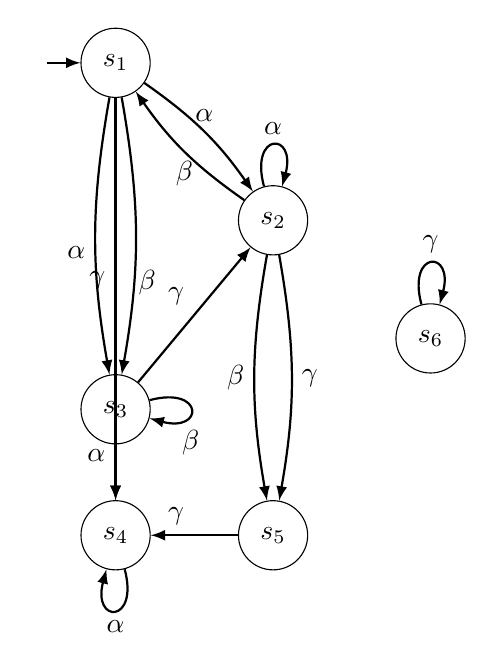
\begin{tikzpicture} [scale=2, every initial by arrow/.style={thick}]
		

		\path
		(\basex,		\basey) 		node[state,init] (s1) 	{$\state_1$} 
		(\basex+2,		\basey+0) 		node[state] (s2) 	{$\state_2$} 
		(\basex+1,		\basey-1.2) 	node[state] (s3) 	{$\state_3$} 
		(\basex,		\basey-2) 		node[state] (s4) 	{$\state_4$} 
		(\basex+2,		\basey-2) 		node[state] (s5) 	{$\state_5$}
		(\basex+3,		\basey-.75) 	node[state] (s6) 	{$\state_6$}
				
		;
		
%		
		\path [bendtrans] 	(s1) 	edge node [midway,above]				{\action} 		(s2);
		\path [bendtrans] 	(s1) 	edge node [near end,above right=-2pt]	{\actionb} 		(s3);
		\path [bendtransr] 	(s1) 	edge node [midway,below left]	{\action} 		(s3);
		\path [trans] 		(s1) 	edge node [midway,above left]	{\actionc} 		(s4);
		\path [bendtrans] 	(s2) 	edge node [midway,below]		{\actionb} 		(s1);
		\path [bendtransr] 	(s2) 	edge node [midway,left]			{\actionb} 		(s5);
		\path [bendtrans] 	(s2) 	edge node [midway,right]		{\actionc} 		(s5);
		\path [trans] 		(s3)	edge node [midway,above left]	{\actionc} 		(s2);
		\path [trans] 		(s3)	edge node [midway,above left]	{\action} 		(s4);
		\path [trans] 		(s5)	edge node [midway,above left]	{\actionc} 		(s4);
		
		\path [trans] 		(s2) 	edge [loop above] node [midway,above] {\action} 	(s2);
		\path [trans] 		(s3) 	edge [loop right] node [midway,below=4pt] {\actionb} 	(s3);
		\path [trans] 		(s4) 	edge [loop below] node [midway,below] {\action} 	(s4);
		\path [trans] 		(s6) 	edge [loop above] node [midway,above] {\actionc} 	(s6);
		
		
		%		midway, at start, near start, very near start, at end, near end, very near end
		
		
	\end{tikzpicture}
\end{document}
	\end{minipage}%
	\begin{minipage}{.5\textwidth}
		\hspace{5mm}
		\documentclass[tikz,preview]{standalone}
%\usepackage{prelude}

%%%%%%%%%%%%%%%%%%%%%%%%%%%%%%%%%%%% PACKAGES %%%%%%%%%%%%%%%%%%%%%%%%%%%%%%%%%%%%%%%%%%

\usepackage{inputenc,fontenc}
\usepackage[a4paper,margin=3cm]{geometry}
\usepackage[english]{babel}
%\usepackage[german]{babel}
%\usepackage[fixlanguage]{babelbib}


\usepackage{bbold}
\usepackage{amsthm}
\usepackage{amsmath}
\usepackage{amssymb} % doteqdot
\usepackage[dvipsnames]{xcolor}
\usepackage{standalone}
\usepackage{tikz}[mode=buildnew]
\usepackage{cite}
\usepackage{xspace}
\usepackage{relsize}
\usepackage{mathtools} % mathclap
%\usepackage{MnSymbol}
\usepackage{hyperref}
\usepackage{url}
\usepackage{listings} % for code
\usepackage[T1]{fontenc} %<
\hypersetup{
	colorlinks,
	citecolor=black,
	filecolor=black,
	linkcolor=black,
	urlcolor=black
}
\usepackage{pgfplots}
\pgfplotsset{compat=1.18}
%\usepackage{courier} %% Sets font for listing as Courier. But also for url and texttt!
\usepackage{listings, xcolor}
\usepackage{graphicx}
\usepackage{subcaption}

\usetikzlibrary{calc}
%\usepackage{xparse} % \newDocumentCommand for multiple optional arguments
%\usepackage{titlecaps}



%%%%%%%%%%%%%%%%%%%%%%%%%%%%%%%%%%%% THEOREMSTYLES %%%%%%%%%%%%%%%%%%%%%%%%%%%%%%%%%%

\theoremstyle{definition}
\newtheorem{definition}{Definition}[section]
\newtheorem{exmp}{Beispiel}[section]
%\AfterEndEnvironment{definition}{\noindent\ignorespaces}

\theoremstyle{theorem}
\newtheorem{theorem}{Satz}[section]
\newtheorem{proposition}{Proposition}[section]
%\AfterEndEnvironment{theorem}{\noindent\ignorespaces}

\theoremstyle{korollary}
\newtheorem{korollary}{Korollar}[section]
%\AfterEndEnvironment{korollary}{\noindent\ignorespaces}


\tikzset{
	mstate/.style={draw, circle, minimum size=.94cm}, 
	gstate/.style={draw, rectangle, minimum size=.8cm},
	varstate/.style={draw,rectangle, rounded corners, minimum size=1}, 
	trans/.style={draw, ->, thick},
	bendtrans/.style={draw, ->, thick, bend left=10},
	bendtransr/.style={draw, ->, thick, bend right=10},
	init/.style={initial, initial distance=6pt, initial text=},
	every loop/.style={min distance=5pt, looseness=8},
	>=latex
}
\usetikzlibrary{automata,positioning}

%auto shift/.style={auto=right,->,
%	to path={ let \p1=(\tikztostart),\p2=(\tikztotarget),
%		\n1={atan2(\y2-\y1,\x2-\x1)},\n2={\n1+180}
%		in ($(\tikztostart.{\n1})!1mm!270:(\tikztotarget.{\n2})$) -- 
%		($(\tikztotarget.{\n2})!1mm!90:(\tikztostart.{\n1})$) \tikztonodes}},

%%%%%%%%%%%%%%%%%%%%%%%%%%%%%%%%%%% MY MACROS %%%%%%%%%%%%%%%%%%%%%%%%%%%%%%%%%%%%%%%%%
%formatting
\newcommand{\comment}[2]{{\color{#1}#2}}
\newcommand{\redcomment}[1]{{\color{red}#1}}
\newcommand{\purpcomment}[1]{{\color{pink}#1}}
\newcommand{\bluecomment}[1]{{\color{blue}#1}}
\newcommand{\mt}[1]{\ensuremath{{#1}}\xspace}
\newcommand{\mynewcommand}[2]{\newcommand{#1}{\mt{#2}}} %% currently not used becaue of ide highlighting
\newcommand{\arr}{\mt{\to}}

%model checking terms
\newcommand{\mimicrel}{\mt{\mathcal{R}}}
\newcommand{\bisimeq}{\mt{\;\!\sim\;\!}}
\newcommand{\simorder}{\mt{\;\!\preceq\;\!}}
\newcommand{\simequiv}{\mt{\;\!\simeq\;\!}} %command already defined
\newcommand{\relts}{\mt{\;\!\bullet_{_{\tiny{TS}}}\;\!}}
\newcommand{\rel}{\mt{\;\!\bullet\;\!}}

%own names
\newcommand{\nm}[1]{#1\xspace}
\newcommand{\mdpN}{\nm{MDP}}
\newcommand{\mdpsN}{\nm{MDPs}}
\newcommand{\viewN}{\nm{view}}
\newcommand{\viewNC}{\nm{View}}
\newcommand{\viewsN}{\nm{views}}
\newcommand{\viewsNC}{\nm{Views}}
\newcommand{\grpfctsubN}{\nm{detached grouping function}}
\newcommand{\grpfctsubNC}{\nm{detached grouping function}}
\newcommand{\grpfctsubNCC}{\nm{Detached Grouping Function}}
\newcommand{\grpfctN}{\nm{grouping function}}
\newcommand{\grpfctNC}{\nm{Grouping function}}
\newcommand{\grpfctNCC}{\nm{Grouping Function}}
\newcommand{\grpfctsN}{\nm{grouping functions}}
\newcommand{\grpfctsNC}{\nm{Grouping functions}}
\newcommand{\grpfctsNCC}{\nm{Grouping Functions}}
\newcommand{\stmimicN}{\nm{state-mimic}}
\newcommand{\stmimicsN}{\nm{state-mimics}}
\newcommand{\stmimickingN}{\nm{state-mimicking}}
\newcommand{\stmimickedN}{\nm{state-mimicked}}
%\newcommand{\chosenphtypeNCC}{\nm{Transition System}}
%\newcommand{\chgphNC}{\nm{Transition system}}
%\newcommand{\chgphN}{\nm{transition system}}
%\newcommand{\chgphsNCC}{\nm{Transition Systems}}
%\newcommand{\chgphsNC}{\nm{Transition systems}}
%\newcommand{\chgphsN}{\nm{transition systems}}
\newcommand{\chgphNCC}{\nm{MDP}}
\newcommand{\chgphNC}{\nm{MDP}}
\newcommand{\chgphN}{\nm{MDP}}
\newcommand{\achgphN}{\nm{an MDP}}
\newcommand{\chgphsNCC}{\nm{MDPs}}
\newcommand{\chgphsNC}{\nm{MDPs}}
\newcommand{\chgphsN}{\nm{MDPs}}
\newcommand{\parllcompN}{\nm{parallel composition}}
\newcommand{\parllcompNC}{\nm{Parallel composition}}
\newcommand{\parllcompNCC}{\nm{Parallel Composition}}
\newcommand{\parllcompsN}{\nm{parallel compositions}}
\newcommand{\parllcompsNC}{\nm{Parallel compositions}}
\newcommand{\parllcompsNCC}{\nm{Parallel Compositions}}
\newcommand{\sccN}{\nm{SCC}}
\newcommand{\sccsN}{\nm{SCCs}}
\newcommand{\bsccN}{\nm{BSCC}}
\newcommand{\bsccsN}{\nm{BSCCs}}
\newcommand{\jgrapht}{\nm{jGraphtT}}

\newcommand{\outactident}{\nm{OutActionsIdent}}

%names
\newcommand{\iffN}{\nm{if and only if}}
\newcommand{\tsN}{\nm{TS}}

%% outactions identical
\newcommand{\outactidentstrong}{\nm{strong}}
\newcommand{\outactidentweak}{\nm{weak}}

% CORE DEFINITIONS
\newcommand{\grpfct}[1][\viewppty]{\mt{F_{#1}}}
\newcommand{\grpfctsub}[1][\viewppty]{\mt{\tilde{F}_{#1}}}
%\newcommand{\grpfctimg}[1]{\mt{{\grpfct}[{#1}]}}
%\newcommand{\fctimg}[2]{\mt{{#1}[{#2}]}}
\newcommand{\eqrelview}{\mt{R}}
\newcommand{\eqclassv}[1][\state]{\mt{\eqclass{#1}{\eqrelview}}}
\newcommand{\eqclasssetv}[1][\states]{\mt{{#1}/\eqrelview}} %OLD: \bigcup_{\state \in \states} \eqclassv
\newcommand{\viewid}{\mt{\mdp}}
\newcommand{\view}[1][\viewppty]{\mt{\viewid_{#1}}}
\newcommand{\imggrp}{\mt{\arbset}}
\newcommand{\imggrpsub}{\mt{X}}
\newcommand{\viewppty}{\mt{\theta}}
\newcommand{\pll}{\mt{\;\!\pllpure\;\!}}
\newcommand{\pllrev}{\mt{\pllpure^{-1}}}
\newcommand{\pllpure}{\mt{||}}
\newcommand{\compselectset}{\mt{Z}}
\newcommand{\compselectpure}{\mt{\pllpure_\compselectset}}
\newcommand{\compselect}{\mt{\;\pllpure_\compselectset\;}}
\newcommand{\remstates}{\mt{\bigcup_{\state \in \states \setminus \states_1}\{\{\state\}\}}}
\newcommand{\nogroupstates}[1][\states_2]{\mt{\bigcup_{\state \in \states \setminus {#1}}\{\{\state\}\}}}
\newcommand{\remelem}{\mt{\bullet}}
\newcommand{\nogroupset}{\mt{\xi}}
\newcommand{\remset}{\mt{\{\remelem\}}}
\newcommand{\gfctpll}{\mt{\grpfct[\pll]}}
\newcommand{\group}{\mt{\top}}
\newcommand{\imggrpbinview}{\mt{\{\remelem, \notppty\}}}
\newcommand{\viewappset}{\mt{\tilde{\states}}}
\newcommand{\hasppty}{\mt{\top}}
\newcommand{\notppty}{\mt{\bot}}
\newcommand{\disregardelem}{\mt{\Delta}}
\newcommand{\disregardelements}{\mt{{\disregardelem_1, \dots, \disregardelem_n}}}



%\newcommand{\mdp}{def}\mdp
%\newcommand{\mdpdef}



% EXAMPLE VIEWS
\newcommand{\pptyatomicprops}{\mt{\atomicprops}}
\newcommand{\pptyinitstates}{\mt{\initstates}}
\newcommand{\pptyinactsetsize}{\mt{|\inacts(\state)|}}
\newcommand{\pptyhasoutact}{\mt{\exists\outact}}
\newcommand{\pptyminoutact}[2]{\mt{#1\leq#2}}
\newcommand{\pptymaxoutact}[2]{\mt{#2\leq#1}}
\newcommand{\pptyspanoutact}[3]{\mt{#1\leq#2\leq#3}}
\newcommand{\pptyoutactsetsize}{\mt{|\outacts(\state)|}}
\newcommand{\pptyoutactsingle}{\mt{|\outacts(\state)|_1}}
\newcommand{\pptystrongoutactident}{\mt{\outacts(\state)_=}}
\newcommand{\pptyweakoutactident}{\mt{\outacts(\state)_\approx}}
\newcommand{\pptyhasinact}{\mt{\exists\inact}}
\newcommand{\pptymininact}[2]{\mt{#1\leq#2}}
\newcommand{\pptymaxinact}[2]{\mt{#2\leq#1}}
\newcommand{\pptyspaninact}[3]{\mt{#1\leq#2\leq#3}}
\newcommand{\pptyinactsingle}{\mt{|\inacts(\state)|_1}}
\newcommand{\pptystronginactident}{\mt{\inacts(\state)_=}}
\newcommand{\pptyweakinactident}{\mt{\inacts(\state)_\approx}}
\newcommand{\pptyparamvalueseq}{\mt{\var = \varval}}
\newcommand{\pptyparamvaluesneq}{\mt{\var \neq \varval}}
\newcommand{\pptyparamdnf}{\mt{VarDNF}}
\newcommand{\pptyparamcnf}{\mt{VarCNF}}
\newcommand{\pptyparamvalueseqopt}{\mt{\var = \varval}}
\newcommand{\pptyparamvalident}{\mt{Var:\varval}}
\newcommand{\pptydistance}{\mt{\distpath}}
\newcommand{\pptydistancerev}{\mt{\distpathrev}}
\newcommand{\pptydistancebi}{\mt{\distpathbi}}
\newcommand{\pptyhascycle}{\mt{\exists\cycle}}
\newcommand{\pptyexactactcycle}{\mt{\{\cycle_{\action,n}\}}}
\newcommand{\pptycycleset}{\mt{\cup{\{\state\}_\cycle}}}
\newcommand{\pptyexactcycle}{\mt{\{\cycle_n\}}}
\newcommand{\pptyscc}{\mt{scc}}
\newcommand{\pptybscc}{\mt{bscc}}
\newcommand{\pptyprop}{\mt{\redcomment{?}}}
\newcommand{\pptyident}{id}


\newcommand{\gfctatomicprops}{\mt{\grpfct[\pptyatomicprops]}}
\newcommand{\gfctinitstates}{\mt{\grpfct[\pptyinitstates]^\hasppty}}
\newcommand{\gfcthasoutaction}{\mt{\grpfct[\pptyhasoutact]^\hasppty}}
\newcommand{\gfctminoutaction}{\mt{\grpfct[\pptyminoutact{\numoutact}{\outact}]^\hasppty}}
\newcommand{\gfctmaxoutaction}{\mt{\grpfct[\pptymaxoutact{\numoutact}{\outact}]^\hasppty}}
\newcommand{\gfctspanoutaction}{\mt{\grpfct[\pptyspanoutact{\numoutactb}{\outact}{\numoutact}]^\hasppty}}
\newcommand{\gfctoutactsetsize}{\mt{\grpfct[\pptyoutactsetsize]}}
\newcommand{\gfctoutactsingle}{\mt{\grpfct[\pptyoutactsingle]^\notppty}}
\newcommand{\gfctstrongoutactident}{\mt{\grpfct[\pptystrongoutactident]}}
\newcommand{\gfctweakoutactident}{\mt{\grpfct[\pptyweakoutactident]}}
\newcommand{\gfcthasinaction}{\mt{\grpfct[\pptyhasinact]^\hasppty}}
\newcommand{\gfctmininaction}{\mt{\grpfct[\pptymininact{\numinact}{\inact}]^\hasppty}}
\newcommand{\gfctmaxinaction}{\mt{\grpfct[\pptymaxinact{\numinact}{\inact}]^\hasppty}}
\newcommand{\gfctspaninaction}{\mt{\grpfct[\pptyspaninact{\numinactb}{\inact}{\numinact}]^\hasppty}}
\newcommand{\gfctinactsetsize}{\mt{\grpfct[\pptyinactsetsize]}}
\newcommand{\gfctinactsingle}{\mt{\grpfct[\pptyinactsingle]^\notppty}}
\newcommand{\gfctstronginactident}{\mt{\grpfct[\pptystronginactident]}}
\newcommand{\gfctweakinactident}{\mt{\grpfct[\pptyweakinactident]}}
\newcommand{\gfctparamvalueseq}{\mt{\grpfct[\pptyparamvalueseq]^\hasppty}}
\newcommand{\gfctparamvaluesneq}{\mt{\grpfct[\pptyparamvaluesneq]^\hasppty}}
\newcommand{\gfctparamdnf}{\mt{\grpfct[\pptyparamdnf]^\hasppty}}
\newcommand{\gfctparamcnf}{\mt{\grpfct[\pptyparamcnf]^\hasppty}}
\newcommand{\gfctparamvalueseqopt}{\mt{\pptyparamvalueseqopt}}
\newcommand{\gfctparamvalident}{\mt{\grpfct[\pptyparamvalident]}}
\newcommand{\gfctdistance}{\mt{\grpfct[\pptydistance]}}
\newcommand{\gfctdistancerev}{\mt{\grpfct[\pptydistancerev]}}
\newcommand{\gfctdistancebi}{\mt{\grpfct[\pptydistancebi]}}
\newcommand{\gfcthascycle}{\mt{\grpfct[\pptyhascycle]}}
\newcommand{\gfctexactcycle}{\mt{\grpfct[\pptyexactcycle]}}
\newcommand{\gfctcycleset}{\mt{\grpfct[\pptycycleset]}}
\newcommand{\gfctexactactcycle}{\mt{\grpfct[\pptyexactactcycle]}}
\newcommand{\gfctscc}{\mt{\grpfct[\pptyscc]}}
\newcommand{\gfctbscc}{\mt{\grpfct[\pptybscc]}}
\newcommand{\gfctprop}{\mt{\grpfct[\pptyprop]}}
\newcommand{\gfctident}{\mt{\grpfct[\pptyident]}}

\newcommand{\gfctsubatomicprops}{\mt{\grpfctsub[\pptyatomicprops]}}
\newcommand{\gfctsubinitstates}{\mt{\grpfctsub[\pptyinitstates]^\hasppty}}
\newcommand{\gfctsubhasoutaction}{\mt{\grpfctsub[\pptyhasoutact]^\hasppty}}
\newcommand{\gfctsubminoutaction}{\mt{\grpfctsub[\pptyminoutact{\numoutact}{\outact}]^\hasppty}}
\newcommand{\gfctsubmaxoutaction}{\mt{\grpfctsub[\pptymaxoutact{\numoutact}{\outact}]^\hasppty}}
\newcommand{\gfctsubspanoutaction}{\mt{\grpfctsub[\pptyspanoutact{\numoutactb}{\outact}{\numoutact}]^\hasppty}}
\newcommand{\gfctsuboutactsetsize}{\mt{\grpfctsub[\pptyoutactsetsize]}}
\newcommand{\gfctsuboutactsingle}{\mt{\grpfctsub[\pptyoutactsingle]^\notppty}}
\newcommand{\gfctsubstrongoutactident}{\mt{\grpfctsub[\pptystrongoutactident]^\hasppty}}
\newcommand{\gfctsubweakoutactident}{\mt{\grpfctsub[\pptyweakoutactident]^\hasppty}}
\newcommand{\gfctsubhasinaction}{\mt{\grpfctsub[\pptyhasinact]}}
\newcommand{\gfctsubmininaction}{\mt{\grpfctsub[\pptymininact{\numinact}{\inact}]}}
\newcommand{\gfctsubmaxinaction}{\mt{\grpfctsub[\pptymaxinact{\numinact}{\inact}]}}
\newcommand{\gfctsubspaninaction}{\mt{\grpfctsub[\pptyspaninact{\numinactb}{\inact}{\numinact}]}}
\newcommand{\gfctsubinactsetsize}{\mt{\grpfctsub[\pptyinactsetsize]^\hasppty}}
\newcommand{\gfctsubinactsingle}{\mt{\grpfctsub[\pptyinactsingle]^\notppty}}
\newcommand{\gfctsubstronginactident}{\mt{\grpfctsub[\pptystronginactident]}}
\newcommand{\gfctsubweakinactident}{\mt{\grpfctsub[\pptyweakinactident]}}
\newcommand{\gfctsubparamvalueseq}{\mt{\grpfctsub[\pptyparamvalueseq]^\hasppty}}
\newcommand{\gfctsubparamvaluesneq}{\mt{\grpfctsub[\pptyparamvaluesneq]^\hasppty}}
\newcommand{\gfctsubparamdnf}{\mt{\grpfctsub[\pptyparamdnf]^\hasppty}}
\newcommand{\gfctsubparamcnf}{\mt{\grpfctsub[\pptyparamcnf]^\hasppty}}
\newcommand{\gfctsubparamvalueseqopt}{\mt{\pptyparamvalueseqopt}}
\newcommand{\gfctsubparamvalident}{\mt{\grpfctsub[\pptyparamvalident]}}
\newcommand{\gfctsubdistance}{\mt{\grpfctsub[\pptydistance]}}
\newcommand{\gfctsubdistancerev}{\mt{\grpfctsub[\pptydistancerev]}}
\newcommand{\gfctsubdistancebi}{\mt{\grpfctsub[\pptydistancebi]}}
\newcommand{\gfctsubhascycle}{\mt{\grpfctsub[\pptyhascycle]^\hasppty}}
\newcommand{\gfctsubexactcycle}{\mt{\grpfctsub[\pptyexactcycle]}}
\newcommand{\gfctsubcycleset}{\mt{\grpfctsub[\pptycycleset]}}
\newcommand{\gfctsubexactactcycle}{\mt{\grpfctsub[\pptyexactactcycle]}}
\newcommand{\gfctsubscc}{\mt{\grpfctsub[\pptyscc]}}
\newcommand{\gfctsubbscc}{\mt{\grpfctsub[\pptybscc]}}
\newcommand{\gfctsubprop}{\mt{\grpfctsub[\pptyprop]}}
\newcommand{\gfctsubident}{\mt{\grpfctsub[\pptyident]}}


\newcommand{\viewatomicprops}{\mt{\view[\pptyatomicprops]}}
\newcommand{\viewinitstates}{\mt{\view[\pptyinitstates]^\hasppty}}
\newcommand{\viewhasoutaction}{\mt{\view[\pptyhasoutact]^\hasppty}}
\newcommand{\viewminoutaction}{\mt{\view[\pptyminoutact{\numoutact}{\outact}]^\hasppty}}
\newcommand{\viewmaxoutaction}{\mt{\view[\pptymaxoutact{\numoutact}{\outact}]^\hasppty}}
\newcommand{\viewspanoutaction}{\mt{\view[\pptyspanoutact{\numoutactb}{\outact}{\numoutact}]^\hasppty}}
\newcommand{\viewoutactsetsize}{\mt{\view[\pptyoutactsetsize]}}
\newcommand{\viewoutactsingle}{\mt{\view[\pptyoutactsingle]^\notppty}}
\newcommand{\viewstrongoutactident}{\mt{\view[\pptystrongoutactident]}}
\newcommand{\viewweakoutactident}{\mt{\view[\pptyweakoutactident]}}
\newcommand{\viewhasinaction}{\mt{\view[\pptyhasinact]^\hasppty}}
\newcommand{\viewmininaction}{\mt{\view[\pptymininact{\numinact}{\inact}]^\hasppty}}
\newcommand{\viewmaxinaction}{\mt{\view[\pptymaxinact{\numinact}{\inact}]^\hasppty}}
\newcommand{\viewspaninaction}{\mt{\view[\pptyspaninact{\numinactb}{\inact}{\numinact}]^\hasppty}}
\newcommand{\viewinactsetsize}{\mt{\view[\pptyinactsetsize]}}
\newcommand{\viewinactsingle}{\mt{\view[\pptyinactsingle]^\notppty}}
\newcommand{\viewstronginactident}{\mt{\view[\pptystronginactident]}}
\newcommand{\viewweakinactident}{\mt{\view[\pptyweakinactident]}}
\newcommand{\viewparamvalueseq}{\mt{\view[\pptyparamvalueseq]}}
\newcommand{\viewparamvaluesneq}{\mt{\view[\pptyparamvaluesneq]}}
\newcommand{\viewparamdnf}{\mt{\view[\pptyparamdnf]^\hasppty}}
\newcommand{\viewparamcnf}{\mt{\view[\pptyparamcnf]^\hasppty}}
\newcommand{\viewparamvalueseqopt}{\mt{\pptyparamvalueseqopt}}
\newcommand{\viewparamvalident}{\mt{\view[\pptyparamvalident]}}
\newcommand{\viewdistance}{\mt{\view[\pptydistance]}}
\newcommand{\viewdistancerev}{\mt{\view[\pptydistancerev]}}
\newcommand{\viewdistancebi}{\mt{\view[\pptydistancebi]}}
\newcommand{\viewhascycle}{\mt{\view[\pptyhascycle]}}
\newcommand{\viewexactcycle}{\mt{\view[\pptyexactcycle]}}
\newcommand{\viewcycleset}{\mt{\view[\pptycycleset]}}
\newcommand{\viewexactactcycle}{\mt{\view[\pptyexactactcycle]}}
\newcommand{\viewscc}{\mt{\view[\pptyscc]}}
\newcommand{\viewbscc}{\mt{\view[\pptybscc]}}
\newcommand{\viewprop}{\mt{\view[\pptyprop]}}
\newcommand{\viewident}{\mt{\view[\pptyident]}}

%\newcommand{\viewatomicprops}{\mt{\view[\atomicprops]}}
%\newcommand{\viewinitstates}{\mt{\view[\initstates]}}
%\newcommand{\viewhasoutaction}{\mt{\view[\pptyhasoutact]}}
%\newcommand{\viewminoutaction}{\mt{\view[\pptyminoutact{\numoutact}{\outact}]}}
%\newcommand{\viewmaxoutaction}{\mt{\view[\pptymaxoutact{\numoutact}{\outact}]}}
%\newcommand{\viewspanoutaction}{\mt{\view[\pptyspanoutact{\numoutactb}{\outact}{\numoutact}]}}
%\newcommand{\viewoutactsetsize}{\mt{\view[\pptyoutactsetsize]}}
%\newcommand{\viewoutactsingle}{\mt{\view[\pptyoutactsingle]}}
%\newcommand{\viewstrongoutactident}{\mt{\view[\outacts(\state)_=]}}
%\newcommand{\viewweakoutactident}{\mt{\view[\outacts(\state)_\approx]}}
%\newcommand{\viewhasinaction}{\mt{\view[\pptyhasinact]}}
%\newcommand{\viewmininaction}{\mt{\view[\pptymininact{\numinact}{\inact}]}}
%\newcommand{\viewmaxinaction}{\mt{\view[\pptymaxinact{\numinact}{\inact}]}}
%\newcommand{\viewspaninaction}{\mt{\view[\pptyspaninact{\numinactb}{\inact}{\numinact}]}}
%\newcommand{\viewinactsetsize}{\mt{\view[\pptyinactsetsize]}}
%\newcommand{\viewinactsingle}{\mt{\view[\pptyinactsingle]}}
%\newcommand{\viewstronginactident}{\mt{\view[\inacts(\state)_=]}}
%\newcommand{\viewweakinactident}{\mt{\view[\inacts(\state)_\approx]}}
%\newcommand{\viewparamvalueseq}{\mt{\view[\var = \varval]}}
%\newcommand{\viewparamvaluesneq}{\mt{\view[\var \neq \varval]}}
%\newcommand{\viewparamdnf}{\mt{\view[VarDNF]}}
%\newcommand{\viewparamcnf}{\mt{\view[VarCNF]}}
%\newcommand{\viewparamvalident}{\mt{\view[\pptyparamvalident]}}
%\newcommand{\viewdistance}{\mt{\view[\pptydistance]}}
%\newcommand{\viewhascycle}{\mt{\view[\exists\cycle]}}
%\newcommand{\viewexactcycle}{\mt{\view[\pptyexactcycle]}}
%\newcommand{\viewcycleset}{\mt{\view[\pptycycleset]}}
%\newcommand{\viewexactactcycle}{\mt{\view[\pptyexactactcycle]}}
%\newcommand{\viewscc}{\mt{\view[scc]}}
%\newcommand{\viewbscc}{\mt{\view[bscc]}}

%actions
\newcommand{\numoutact}{\mt{n}}
\newcommand{\numoutactb}{\mt{m}}
\newcommand{\numinact}{\mt{n}}
\newcommand{\numinactb}{\mt{m}}

\newcommand{\predmaxoutact}[1][\numoutact]{\mt{Q_{\outact\leq#1}(\state,\state_1, \dots, \state_{#1+1})}}
\newcommand{\predminoutact}[1][\numoutact]{\mt{Q_{#1\leq\outact}(\state,\state_1, \dots, \state_{#1})}}
\newcommand{\formoutact}[1][\state]{\mt{C_{#1,\outact}}}
\newcommand{\predmaxinact}[1][\numinact]{\mt{Q_{\inact\leq#1}(\state,\state_1, \dots, \state_{#1+1})}}
\newcommand{\predmininact}[1][\numinact]{\mt{Q_{#1\leq\inact}(\state,\state_1, \dots, \state_{#1})}}

\newcommand{\outact}[1][\action]{\mt{\overrightarrow{#1}}}
\newcommand{\outacts}{\mt{\overrightarrow{\actions}}}
\newcommand{\inact}{\mt{\overleftarrow{\action}}}
\newcommand{\inacts}[1][\action]{\mt{\overleftarrow{#1}}}

%%Parameters
\newcommand{\vars}[1][\mdp]{\mt{V\!ar_{#1}}}
\newcommand{\var}{\mt{x}}
\newcommand{\varstate}[1][]{\mt{\var_{\state#1}}}
\newcommand{\varval}{\mt{a}}
\newcommand{\vareval}[1][\mdp]{\mt{V\!arEval_{#1}}}
\newcommand{\varevalimg}[1][\mdp]{\mt{\vareval[#1][\states,\vars]}}
\newcommand{\varevalimgset}{\mt{\arbset}}
\newcommand{\someparam}{\mt{\tilde{x}}}
\newcommand{\eqorneq}{\mt{\;\doteqdot\;}}
\newcommand{\varstyle}[2]{\mt{\langle#1,#2\rangle}}




%\makeatletter
%\newcommand{\overleftrightsmallarrow}{\mathpalette{\overarrowsmall@\leftrightarrowfill@}}
%\newcommand{\overrightsmallarrow}{\mathpalette{\overarrowsmall@\rightarrowfill@}}
%\newcommand{\overleftsmallarrow}{\mathpalette{\overarrowsmall@\leftarrowfill@}}
%\newcommand{\overarrowsmall@}[3]{%
%	\vbox{%
%		\ialign{%
%			##\crcr
%			#1{\smaller@style{#2}}\crcr
%			\noalign{\nointerlineskip}%
%			$\m@th\hfil#2#3\hfil$\crcr
%		}%
%	}%
%}
%\def\smaller@style#1{%
%	\ifx#1\displaystyle\scriptstyle\else
%	\ifx#1\textstyle\scriptstyle\else
%	\scriptscriptstyle
%	\fi
%	\fi
%}
%\makeatother
%\newcommand{\te}[1]{\overleftrightsmallarrow{#1}}

% Distance
\newcommand{\fctdist}{\mt{distance}}
\newcommand{\fctdistdefault}{\mt{\fctdist(\chgph, \smstates, \grandist)}}
\newcommand{\distval}{\mt{d}}
\newcommand{\grandist}{\mt{n}}
\let\path\oldpath
\newcommand{\path}{\mt{P}}
\newcommand{\pathbi}{\mt{\bar{\path}}}
\newcommand{\pathsecfull}{\mt{(\state_0, \action_0, \state_1, \action_1, \dots, \action_{n}, \state_{n+1})}}
\newcommand{\lenpath}{\mt{len}}
\newcommand{\pfirst}{\mt{first}}
\newcommand{\plast}{\mt{last}}
\newcommand{\pathset}{\mt{\path_\chgph}}
\newcommand{\pathbiset}{\mt{\pathbi_\chgph}}
\newcommand{\distpath}{\mt{\overrightarrow{dist}}}
\newcommand{\distpathrev}{\mt{\overleftarrow{dist}}}
\newcommand{\distpathbi}{\mt{\overline{dist}}}
%Cycles
\newcommand{\cyclesecfull}{\mt{(\state_0, \action_0, \state_1, \action_1, \dots, \action_{n-1}, \state_0)}}
\newcommand{\fctfindcycles}{\mt{findCycles}}
\newcommand{\cycle}{\mt{C}}
\newcommand{\cycleset}{\mt{\cycle_{\mdp, n}}}
\newcommand{\lencycle}{\mt{len}}
% strongly connected components
\newcommand{\scc}{\mt{T}}
\newcommand{\setscc}{\mt{SCC_{\chgph,n}}}
\newcommand{\setbscc}{\mt{BSCC_{\chgph,n}}}

% properties
\newcommand{\propfct}{\mt{f}}

% all Systems
\newcommand{\chgph}{\mt{\mdp}}
\newcommand{\chgphtuple}{\mt{\mdptuple}}
\newcommand{\chgphtupledist}{\mt{\mdptupledist}}

\newcommand{\states}{\mt{S}}
\newcommand{\actions}{\mt{Act}}
\newcommand{\atomicprops}{\mt{AP}}
\newcommand{\labelingfct}{\mt{L}}
\newcommand{\init}{\mt{\initdistrib}} % use MDP % refers to the underlying set
\newcommand{\trans}{\mt{\probtfunc}} % use MDP % refers to the underlying set
\newcommand{\smstates}{\mt{\tilde{\states}}}


\newcommand{\state}{\mt{s}}
\newcommand{\action}{\mt{\alpha}}
\newcommand{\actionb}{\mt{\beta}}
\newcommand{\actionc}{\mt{\gamma}}
\newcommand{\smstate}{\mt{\tilde{\state}}}



% transition sysstems
\newcommand{\ts}{\mt{TS}}
\newcommand{\transitionrel}{\mt{\longrightarrow}}
\newcommand{\initstates}{\mt{I}}
\newcommand{\transitionsystem}{\mt
	{(\states, \actions, \transitionrel, \initstates, \atomicprops, \labelingfct)}
}
\newcommand{\tstupledist}{\mt{(\states', \actions',\transitionrel', \initstates', \labelingfct')}}


%Markov chains and MDP
\newcommand{\mdp}{\mt{\autm}}
\newcommand{\mdptuple}{\mt{(\states, \actions, \probtfunc, \initdistrib, \atomicprops, \labelingfct)}}
\newcommand{\mdptupledist}{\mt{(\states', \actions', \probtfunc', \initdistrib', \atomicprops', \labelingfct')}}
\newcommand{\autm}{\mt{\mathcal{M}}}
\newcommand{\probtfunc}{\mt{\textbf{P}}}
\newcommand{\initdistrib}{\mt{\iota_{init}}}


%maths
\newcommand{\powerset}[1]{\mt{\mathcal{P}(#1)}}
\newcommand{\eqclass}[2]{\mt{[#1]_{#2}}}%{\mt{#1 / #2}}
\newcommand{\impr}{\mt{\hspace{3mm}\Rightarrow\hspace{2mm}}}
\newcommand{\impl}{\mt{\hspace{3mm}\Leftarrow\hspace{2mm}}}
\newcommand{\natnums}{\mt{\mathbb{N}}} 
\newcommand{\realnums}{\mt{\mathbb{R}}}
\newcommand{\intmodn}[1][n]{\mt{\mathbb{Z}_{#1}}}
\newcommand{\arbset}{\mt{M}}
\newcommand{\bigsum}[2][]{\mt{\mathlarger{\sum}_{#2}^{#1}}}
\newcommand{\bbigsum}[2][]{\mt{\mathlarger{\mathlarger{\sum}}_{#2}^{#1}}}
\newcommand{\invimage}[2]{#1^{\mt{-1}(#2)}}
\newcommand{\img}{\mt{Img}}
\newcommand{\cond}{\mt{\,|\,}}

%tickz
%% \definecolor{darkred}{RGB}{196, 42, 42}

%implementation
\newcommand{\pmcvis}{\nm{PMC-Vis}}





\begin{document}
	\newcommand{\basex}{0}
	\newcommand{\basey}{0}
	\newcommand{\createstate}[3]{\node[draw, circle, minimum size=1cm] (#1) at (#2) {#3}}
	
	
	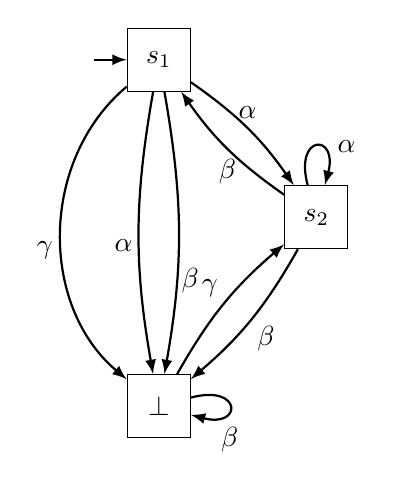
\begin{tikzpicture} [scale=2, every initial by arrow/.style={thick}]
		
		
		\path
		(\basex,		\basey) 		node[gstate,init] (s1) 	{$\state_1$} 
		(\basex+2,		\basey+0) 		node[gstate] (s2) 	{$\state_2$} 
		(\basex+1,		\basey-1.2) 	node[gstate] (sbot) 	{$\notppty$} 
		
		
		;
		
		%		
		\path [bendtrans] 	(s1) 	edge node [midway,above]				{\action} 		(s2);
		\path [bendtrans] 	(s1) 	edge node [near end,above right=-2pt]	{\actionb} 		(sbot);
		\path [bendtransr] 	(s1) 	edge node [midway,below left=-2pt]	{\action} 		(sbot);
		\path [trans, bend right=50] 	(s1) 	edge node [midway,below left=-1pt]	{\actionc} 		(sbot);
		\path [bendtrans] 	(s2) 	edge node [midway,below]		{\actionb} 		(s1);
		\path [bendtrans] 	(s2) 	edge node [midway,below right=-2pt]		{\actionb} 		(sbot);
		\path [bendtrans] 		(sbot)	edge node [midway,above left=-2pt]	{\actionc} 		(s2);

		
		\path [trans] 		(s2) 	edge [loop above] node [midway,right=4pt] {\action} 	(s2);
		\path [trans] 		(sbot) 	edge [loop right] node [midway,below=4pt] {\actionb} 	(sbot);

		
		
		%		midway, at start, near start, very near start, at end, near end, very near end
		
		
	\end{tikzpicture}
\end{document}
	\end{minipage}
	\caption{Simplified representations of \mdp (left) and the \viewN $\view[\pptyminoutact{2}{\outact}]$ on it (right)}
	\label{fig:outActMinAfter}  
\end{figure}


Since we already defined \grpfctsN and hence views for a required minimal and maximal amount of times an action has to be outgoing it is now easily possible to define a view that groups states where the amount of outgoing actions is at least \numoutact and at most \numoutactb. 

\begin{definition}
	Let $\chgph = \chgphtuple$ be \achgphN and $\action \in \actions$. The view 
	\viewspanoutaction is defined by its \grpfctN $\gfctspanoutaction : \states \to \arbset$ with
	
	\[
	\state \mapsto
	\begin{cases}
			\group,				& \text{if } \exists \state_1, \dots, \state_\numoutactb \in \states: \predminoutact[\numoutactb] \\ &\text{and } \forall \state_1, \dots, \state_{\numoutact+1} \in \states: \predmaxoutact \\
			\remelem,          	& \text{otherwise}
		\end{cases}
	\]
	
	where $\imggrp := \imggrpbinview$
%	\actions \cup \remset$ 
	and $\numoutactb, \numoutact \in \natnums$ are the minimal and maximal number of transitions with action \action in order for state to be grouped. The predicates \predminoutact and \predmaxoutact are the predicates from Definition \ref{def:minoutaction} and Definition \ref{def:viewmaxoutaction} respectively.
\end{definition}

\begin{figure}[h]
	\begin{minipage}{.5\textwidth}
		\hspace{5mm}
		\documentclass[tikz,preview]{standalone}
%\usepackage{prelude}

%%%%%%%%%%%%%%%%%%%%%%%%%%%%%%%%%%%% PACKAGES %%%%%%%%%%%%%%%%%%%%%%%%%%%%%%%%%%%%%%%%%%

\usepackage{inputenc,fontenc}
\usepackage[a4paper,margin=3cm]{geometry}
\usepackage[english]{babel}
%\usepackage[german]{babel}
%\usepackage[fixlanguage]{babelbib}


\usepackage{bbold}
\usepackage{amsthm}
\usepackage{amsmath}
\usepackage{amssymb} % doteqdot
\usepackage[dvipsnames]{xcolor}
\usepackage{standalone}
\usepackage{tikz}[mode=buildnew]
\usepackage{cite}
\usepackage{xspace}
\usepackage{relsize}
\usepackage{mathtools} % mathclap
%\usepackage{MnSymbol}
\usepackage{hyperref}
\usepackage{url}
\usepackage{listings} % for code
\usepackage[T1]{fontenc} %<
\hypersetup{
	colorlinks,
	citecolor=black,
	filecolor=black,
	linkcolor=black,
	urlcolor=black
}
\usepackage{pgfplots}
\pgfplotsset{compat=1.18}
%\usepackage{courier} %% Sets font for listing as Courier. But also for url and texttt!
\usepackage{listings, xcolor}
\usepackage{graphicx}
\usepackage{subcaption}

\usetikzlibrary{calc}
%\usepackage{xparse} % \newDocumentCommand for multiple optional arguments
%\usepackage{titlecaps}



%%%%%%%%%%%%%%%%%%%%%%%%%%%%%%%%%%%% THEOREMSTYLES %%%%%%%%%%%%%%%%%%%%%%%%%%%%%%%%%%

\theoremstyle{definition}
\newtheorem{definition}{Definition}[section]
\newtheorem{exmp}{Beispiel}[section]
%\AfterEndEnvironment{definition}{\noindent\ignorespaces}

\theoremstyle{theorem}
\newtheorem{theorem}{Satz}[section]
\newtheorem{proposition}{Proposition}[section]
%\AfterEndEnvironment{theorem}{\noindent\ignorespaces}

\theoremstyle{korollary}
\newtheorem{korollary}{Korollar}[section]
%\AfterEndEnvironment{korollary}{\noindent\ignorespaces}


\tikzset{
	mstate/.style={draw, circle, minimum size=.94cm}, 
	gstate/.style={draw, rectangle, minimum size=.8cm},
	varstate/.style={draw,rectangle, rounded corners, minimum size=1}, 
	trans/.style={draw, ->, thick},
	bendtrans/.style={draw, ->, thick, bend left=10},
	bendtransr/.style={draw, ->, thick, bend right=10},
	init/.style={initial, initial distance=6pt, initial text=},
	every loop/.style={min distance=5pt, looseness=8},
	>=latex
}
\usetikzlibrary{automata,positioning}

%auto shift/.style={auto=right,->,
%	to path={ let \p1=(\tikztostart),\p2=(\tikztotarget),
%		\n1={atan2(\y2-\y1,\x2-\x1)},\n2={\n1+180}
%		in ($(\tikztostart.{\n1})!1mm!270:(\tikztotarget.{\n2})$) -- 
%		($(\tikztotarget.{\n2})!1mm!90:(\tikztostart.{\n1})$) \tikztonodes}},

%%%%%%%%%%%%%%%%%%%%%%%%%%%%%%%%%%% MY MACROS %%%%%%%%%%%%%%%%%%%%%%%%%%%%%%%%%%%%%%%%%
%formatting
\newcommand{\comment}[2]{{\color{#1}#2}}
\newcommand{\redcomment}[1]{{\color{red}#1}}
\newcommand{\purpcomment}[1]{{\color{pink}#1}}
\newcommand{\bluecomment}[1]{{\color{blue}#1}}
\newcommand{\mt}[1]{\ensuremath{{#1}}\xspace}
\newcommand{\mynewcommand}[2]{\newcommand{#1}{\mt{#2}}} %% currently not used becaue of ide highlighting
\newcommand{\arr}{\mt{\to}}

%model checking terms
\newcommand{\mimicrel}{\mt{\mathcal{R}}}
\newcommand{\bisimeq}{\mt{\;\!\sim\;\!}}
\newcommand{\simorder}{\mt{\;\!\preceq\;\!}}
\newcommand{\simequiv}{\mt{\;\!\simeq\;\!}} %command already defined
\newcommand{\relts}{\mt{\;\!\bullet_{_{\tiny{TS}}}\;\!}}
\newcommand{\rel}{\mt{\;\!\bullet\;\!}}

%own names
\newcommand{\nm}[1]{#1\xspace}
\newcommand{\mdpN}{\nm{MDP}}
\newcommand{\mdpsN}{\nm{MDPs}}
\newcommand{\viewN}{\nm{view}}
\newcommand{\viewNC}{\nm{View}}
\newcommand{\viewsN}{\nm{views}}
\newcommand{\viewsNC}{\nm{Views}}
\newcommand{\grpfctsubN}{\nm{detached grouping function}}
\newcommand{\grpfctsubNC}{\nm{detached grouping function}}
\newcommand{\grpfctsubNCC}{\nm{Detached Grouping Function}}
\newcommand{\grpfctN}{\nm{grouping function}}
\newcommand{\grpfctNC}{\nm{Grouping function}}
\newcommand{\grpfctNCC}{\nm{Grouping Function}}
\newcommand{\grpfctsN}{\nm{grouping functions}}
\newcommand{\grpfctsNC}{\nm{Grouping functions}}
\newcommand{\grpfctsNCC}{\nm{Grouping Functions}}
\newcommand{\stmimicN}{\nm{state-mimic}}
\newcommand{\stmimicsN}{\nm{state-mimics}}
\newcommand{\stmimickingN}{\nm{state-mimicking}}
\newcommand{\stmimickedN}{\nm{state-mimicked}}
%\newcommand{\chosenphtypeNCC}{\nm{Transition System}}
%\newcommand{\chgphNC}{\nm{Transition system}}
%\newcommand{\chgphN}{\nm{transition system}}
%\newcommand{\chgphsNCC}{\nm{Transition Systems}}
%\newcommand{\chgphsNC}{\nm{Transition systems}}
%\newcommand{\chgphsN}{\nm{transition systems}}
\newcommand{\chgphNCC}{\nm{MDP}}
\newcommand{\chgphNC}{\nm{MDP}}
\newcommand{\chgphN}{\nm{MDP}}
\newcommand{\achgphN}{\nm{an MDP}}
\newcommand{\chgphsNCC}{\nm{MDPs}}
\newcommand{\chgphsNC}{\nm{MDPs}}
\newcommand{\chgphsN}{\nm{MDPs}}
\newcommand{\parllcompN}{\nm{parallel composition}}
\newcommand{\parllcompNC}{\nm{Parallel composition}}
\newcommand{\parllcompNCC}{\nm{Parallel Composition}}
\newcommand{\parllcompsN}{\nm{parallel compositions}}
\newcommand{\parllcompsNC}{\nm{Parallel compositions}}
\newcommand{\parllcompsNCC}{\nm{Parallel Compositions}}
\newcommand{\sccN}{\nm{SCC}}
\newcommand{\sccsN}{\nm{SCCs}}
\newcommand{\bsccN}{\nm{BSCC}}
\newcommand{\bsccsN}{\nm{BSCCs}}
\newcommand{\jgrapht}{\nm{jGraphtT}}

\newcommand{\outactident}{\nm{OutActionsIdent}}

%names
\newcommand{\iffN}{\nm{if and only if}}
\newcommand{\tsN}{\nm{TS}}

%% outactions identical
\newcommand{\outactidentstrong}{\nm{strong}}
\newcommand{\outactidentweak}{\nm{weak}}

% CORE DEFINITIONS
\newcommand{\grpfct}[1][\viewppty]{\mt{F_{#1}}}
\newcommand{\grpfctsub}[1][\viewppty]{\mt{\tilde{F}_{#1}}}
%\newcommand{\grpfctimg}[1]{\mt{{\grpfct}[{#1}]}}
%\newcommand{\fctimg}[2]{\mt{{#1}[{#2}]}}
\newcommand{\eqrelview}{\mt{R}}
\newcommand{\eqclassv}[1][\state]{\mt{\eqclass{#1}{\eqrelview}}}
\newcommand{\eqclasssetv}[1][\states]{\mt{{#1}/\eqrelview}} %OLD: \bigcup_{\state \in \states} \eqclassv
\newcommand{\viewid}{\mt{\mdp}}
\newcommand{\view}[1][\viewppty]{\mt{\viewid_{#1}}}
\newcommand{\imggrp}{\mt{\arbset}}
\newcommand{\imggrpsub}{\mt{X}}
\newcommand{\viewppty}{\mt{\theta}}
\newcommand{\pll}{\mt{\;\!\pllpure\;\!}}
\newcommand{\pllrev}{\mt{\pllpure^{-1}}}
\newcommand{\pllpure}{\mt{||}}
\newcommand{\compselectset}{\mt{Z}}
\newcommand{\compselectpure}{\mt{\pllpure_\compselectset}}
\newcommand{\compselect}{\mt{\;\pllpure_\compselectset\;}}
\newcommand{\remstates}{\mt{\bigcup_{\state \in \states \setminus \states_1}\{\{\state\}\}}}
\newcommand{\nogroupstates}[1][\states_2]{\mt{\bigcup_{\state \in \states \setminus {#1}}\{\{\state\}\}}}
\newcommand{\remelem}{\mt{\bullet}}
\newcommand{\nogroupset}{\mt{\xi}}
\newcommand{\remset}{\mt{\{\remelem\}}}
\newcommand{\gfctpll}{\mt{\grpfct[\pll]}}
\newcommand{\group}{\mt{\top}}
\newcommand{\imggrpbinview}{\mt{\{\remelem, \notppty\}}}
\newcommand{\viewappset}{\mt{\tilde{\states}}}
\newcommand{\hasppty}{\mt{\top}}
\newcommand{\notppty}{\mt{\bot}}
\newcommand{\disregardelem}{\mt{\Delta}}
\newcommand{\disregardelements}{\mt{{\disregardelem_1, \dots, \disregardelem_n}}}



%\newcommand{\mdp}{def}\mdp
%\newcommand{\mdpdef}



% EXAMPLE VIEWS
\newcommand{\pptyatomicprops}{\mt{\atomicprops}}
\newcommand{\pptyinitstates}{\mt{\initstates}}
\newcommand{\pptyinactsetsize}{\mt{|\inacts(\state)|}}
\newcommand{\pptyhasoutact}{\mt{\exists\outact}}
\newcommand{\pptyminoutact}[2]{\mt{#1\leq#2}}
\newcommand{\pptymaxoutact}[2]{\mt{#2\leq#1}}
\newcommand{\pptyspanoutact}[3]{\mt{#1\leq#2\leq#3}}
\newcommand{\pptyoutactsetsize}{\mt{|\outacts(\state)|}}
\newcommand{\pptyoutactsingle}{\mt{|\outacts(\state)|_1}}
\newcommand{\pptystrongoutactident}{\mt{\outacts(\state)_=}}
\newcommand{\pptyweakoutactident}{\mt{\outacts(\state)_\approx}}
\newcommand{\pptyhasinact}{\mt{\exists\inact}}
\newcommand{\pptymininact}[2]{\mt{#1\leq#2}}
\newcommand{\pptymaxinact}[2]{\mt{#2\leq#1}}
\newcommand{\pptyspaninact}[3]{\mt{#1\leq#2\leq#3}}
\newcommand{\pptyinactsingle}{\mt{|\inacts(\state)|_1}}
\newcommand{\pptystronginactident}{\mt{\inacts(\state)_=}}
\newcommand{\pptyweakinactident}{\mt{\inacts(\state)_\approx}}
\newcommand{\pptyparamvalueseq}{\mt{\var = \varval}}
\newcommand{\pptyparamvaluesneq}{\mt{\var \neq \varval}}
\newcommand{\pptyparamdnf}{\mt{VarDNF}}
\newcommand{\pptyparamcnf}{\mt{VarCNF}}
\newcommand{\pptyparamvalueseqopt}{\mt{\var = \varval}}
\newcommand{\pptyparamvalident}{\mt{Var:\varval}}
\newcommand{\pptydistance}{\mt{\distpath}}
\newcommand{\pptydistancerev}{\mt{\distpathrev}}
\newcommand{\pptydistancebi}{\mt{\distpathbi}}
\newcommand{\pptyhascycle}{\mt{\exists\cycle}}
\newcommand{\pptyexactactcycle}{\mt{\{\cycle_{\action,n}\}}}
\newcommand{\pptycycleset}{\mt{\cup{\{\state\}_\cycle}}}
\newcommand{\pptyexactcycle}{\mt{\{\cycle_n\}}}
\newcommand{\pptyscc}{\mt{scc}}
\newcommand{\pptybscc}{\mt{bscc}}
\newcommand{\pptyprop}{\mt{\redcomment{?}}}
\newcommand{\pptyident}{id}


\newcommand{\gfctatomicprops}{\mt{\grpfct[\pptyatomicprops]}}
\newcommand{\gfctinitstates}{\mt{\grpfct[\pptyinitstates]^\hasppty}}
\newcommand{\gfcthasoutaction}{\mt{\grpfct[\pptyhasoutact]^\hasppty}}
\newcommand{\gfctminoutaction}{\mt{\grpfct[\pptyminoutact{\numoutact}{\outact}]^\hasppty}}
\newcommand{\gfctmaxoutaction}{\mt{\grpfct[\pptymaxoutact{\numoutact}{\outact}]^\hasppty}}
\newcommand{\gfctspanoutaction}{\mt{\grpfct[\pptyspanoutact{\numoutactb}{\outact}{\numoutact}]^\hasppty}}
\newcommand{\gfctoutactsetsize}{\mt{\grpfct[\pptyoutactsetsize]}}
\newcommand{\gfctoutactsingle}{\mt{\grpfct[\pptyoutactsingle]^\notppty}}
\newcommand{\gfctstrongoutactident}{\mt{\grpfct[\pptystrongoutactident]}}
\newcommand{\gfctweakoutactident}{\mt{\grpfct[\pptyweakoutactident]}}
\newcommand{\gfcthasinaction}{\mt{\grpfct[\pptyhasinact]^\hasppty}}
\newcommand{\gfctmininaction}{\mt{\grpfct[\pptymininact{\numinact}{\inact}]^\hasppty}}
\newcommand{\gfctmaxinaction}{\mt{\grpfct[\pptymaxinact{\numinact}{\inact}]^\hasppty}}
\newcommand{\gfctspaninaction}{\mt{\grpfct[\pptyspaninact{\numinactb}{\inact}{\numinact}]^\hasppty}}
\newcommand{\gfctinactsetsize}{\mt{\grpfct[\pptyinactsetsize]}}
\newcommand{\gfctinactsingle}{\mt{\grpfct[\pptyinactsingle]^\notppty}}
\newcommand{\gfctstronginactident}{\mt{\grpfct[\pptystronginactident]}}
\newcommand{\gfctweakinactident}{\mt{\grpfct[\pptyweakinactident]}}
\newcommand{\gfctparamvalueseq}{\mt{\grpfct[\pptyparamvalueseq]^\hasppty}}
\newcommand{\gfctparamvaluesneq}{\mt{\grpfct[\pptyparamvaluesneq]^\hasppty}}
\newcommand{\gfctparamdnf}{\mt{\grpfct[\pptyparamdnf]^\hasppty}}
\newcommand{\gfctparamcnf}{\mt{\grpfct[\pptyparamcnf]^\hasppty}}
\newcommand{\gfctparamvalueseqopt}{\mt{\pptyparamvalueseqopt}}
\newcommand{\gfctparamvalident}{\mt{\grpfct[\pptyparamvalident]}}
\newcommand{\gfctdistance}{\mt{\grpfct[\pptydistance]}}
\newcommand{\gfctdistancerev}{\mt{\grpfct[\pptydistancerev]}}
\newcommand{\gfctdistancebi}{\mt{\grpfct[\pptydistancebi]}}
\newcommand{\gfcthascycle}{\mt{\grpfct[\pptyhascycle]}}
\newcommand{\gfctexactcycle}{\mt{\grpfct[\pptyexactcycle]}}
\newcommand{\gfctcycleset}{\mt{\grpfct[\pptycycleset]}}
\newcommand{\gfctexactactcycle}{\mt{\grpfct[\pptyexactactcycle]}}
\newcommand{\gfctscc}{\mt{\grpfct[\pptyscc]}}
\newcommand{\gfctbscc}{\mt{\grpfct[\pptybscc]}}
\newcommand{\gfctprop}{\mt{\grpfct[\pptyprop]}}
\newcommand{\gfctident}{\mt{\grpfct[\pptyident]}}

\newcommand{\gfctsubatomicprops}{\mt{\grpfctsub[\pptyatomicprops]}}
\newcommand{\gfctsubinitstates}{\mt{\grpfctsub[\pptyinitstates]^\hasppty}}
\newcommand{\gfctsubhasoutaction}{\mt{\grpfctsub[\pptyhasoutact]^\hasppty}}
\newcommand{\gfctsubminoutaction}{\mt{\grpfctsub[\pptyminoutact{\numoutact}{\outact}]^\hasppty}}
\newcommand{\gfctsubmaxoutaction}{\mt{\grpfctsub[\pptymaxoutact{\numoutact}{\outact}]^\hasppty}}
\newcommand{\gfctsubspanoutaction}{\mt{\grpfctsub[\pptyspanoutact{\numoutactb}{\outact}{\numoutact}]^\hasppty}}
\newcommand{\gfctsuboutactsetsize}{\mt{\grpfctsub[\pptyoutactsetsize]}}
\newcommand{\gfctsuboutactsingle}{\mt{\grpfctsub[\pptyoutactsingle]^\notppty}}
\newcommand{\gfctsubstrongoutactident}{\mt{\grpfctsub[\pptystrongoutactident]^\hasppty}}
\newcommand{\gfctsubweakoutactident}{\mt{\grpfctsub[\pptyweakoutactident]^\hasppty}}
\newcommand{\gfctsubhasinaction}{\mt{\grpfctsub[\pptyhasinact]}}
\newcommand{\gfctsubmininaction}{\mt{\grpfctsub[\pptymininact{\numinact}{\inact}]}}
\newcommand{\gfctsubmaxinaction}{\mt{\grpfctsub[\pptymaxinact{\numinact}{\inact}]}}
\newcommand{\gfctsubspaninaction}{\mt{\grpfctsub[\pptyspaninact{\numinactb}{\inact}{\numinact}]}}
\newcommand{\gfctsubinactsetsize}{\mt{\grpfctsub[\pptyinactsetsize]^\hasppty}}
\newcommand{\gfctsubinactsingle}{\mt{\grpfctsub[\pptyinactsingle]^\notppty}}
\newcommand{\gfctsubstronginactident}{\mt{\grpfctsub[\pptystronginactident]}}
\newcommand{\gfctsubweakinactident}{\mt{\grpfctsub[\pptyweakinactident]}}
\newcommand{\gfctsubparamvalueseq}{\mt{\grpfctsub[\pptyparamvalueseq]^\hasppty}}
\newcommand{\gfctsubparamvaluesneq}{\mt{\grpfctsub[\pptyparamvaluesneq]^\hasppty}}
\newcommand{\gfctsubparamdnf}{\mt{\grpfctsub[\pptyparamdnf]^\hasppty}}
\newcommand{\gfctsubparamcnf}{\mt{\grpfctsub[\pptyparamcnf]^\hasppty}}
\newcommand{\gfctsubparamvalueseqopt}{\mt{\pptyparamvalueseqopt}}
\newcommand{\gfctsubparamvalident}{\mt{\grpfctsub[\pptyparamvalident]}}
\newcommand{\gfctsubdistance}{\mt{\grpfctsub[\pptydistance]}}
\newcommand{\gfctsubdistancerev}{\mt{\grpfctsub[\pptydistancerev]}}
\newcommand{\gfctsubdistancebi}{\mt{\grpfctsub[\pptydistancebi]}}
\newcommand{\gfctsubhascycle}{\mt{\grpfctsub[\pptyhascycle]^\hasppty}}
\newcommand{\gfctsubexactcycle}{\mt{\grpfctsub[\pptyexactcycle]}}
\newcommand{\gfctsubcycleset}{\mt{\grpfctsub[\pptycycleset]}}
\newcommand{\gfctsubexactactcycle}{\mt{\grpfctsub[\pptyexactactcycle]}}
\newcommand{\gfctsubscc}{\mt{\grpfctsub[\pptyscc]}}
\newcommand{\gfctsubbscc}{\mt{\grpfctsub[\pptybscc]}}
\newcommand{\gfctsubprop}{\mt{\grpfctsub[\pptyprop]}}
\newcommand{\gfctsubident}{\mt{\grpfctsub[\pptyident]}}


\newcommand{\viewatomicprops}{\mt{\view[\pptyatomicprops]}}
\newcommand{\viewinitstates}{\mt{\view[\pptyinitstates]^\hasppty}}
\newcommand{\viewhasoutaction}{\mt{\view[\pptyhasoutact]^\hasppty}}
\newcommand{\viewminoutaction}{\mt{\view[\pptyminoutact{\numoutact}{\outact}]^\hasppty}}
\newcommand{\viewmaxoutaction}{\mt{\view[\pptymaxoutact{\numoutact}{\outact}]^\hasppty}}
\newcommand{\viewspanoutaction}{\mt{\view[\pptyspanoutact{\numoutactb}{\outact}{\numoutact}]^\hasppty}}
\newcommand{\viewoutactsetsize}{\mt{\view[\pptyoutactsetsize]}}
\newcommand{\viewoutactsingle}{\mt{\view[\pptyoutactsingle]^\notppty}}
\newcommand{\viewstrongoutactident}{\mt{\view[\pptystrongoutactident]}}
\newcommand{\viewweakoutactident}{\mt{\view[\pptyweakoutactident]}}
\newcommand{\viewhasinaction}{\mt{\view[\pptyhasinact]^\hasppty}}
\newcommand{\viewmininaction}{\mt{\view[\pptymininact{\numinact}{\inact}]^\hasppty}}
\newcommand{\viewmaxinaction}{\mt{\view[\pptymaxinact{\numinact}{\inact}]^\hasppty}}
\newcommand{\viewspaninaction}{\mt{\view[\pptyspaninact{\numinactb}{\inact}{\numinact}]^\hasppty}}
\newcommand{\viewinactsetsize}{\mt{\view[\pptyinactsetsize]}}
\newcommand{\viewinactsingle}{\mt{\view[\pptyinactsingle]^\notppty}}
\newcommand{\viewstronginactident}{\mt{\view[\pptystronginactident]}}
\newcommand{\viewweakinactident}{\mt{\view[\pptyweakinactident]}}
\newcommand{\viewparamvalueseq}{\mt{\view[\pptyparamvalueseq]}}
\newcommand{\viewparamvaluesneq}{\mt{\view[\pptyparamvaluesneq]}}
\newcommand{\viewparamdnf}{\mt{\view[\pptyparamdnf]^\hasppty}}
\newcommand{\viewparamcnf}{\mt{\view[\pptyparamcnf]^\hasppty}}
\newcommand{\viewparamvalueseqopt}{\mt{\pptyparamvalueseqopt}}
\newcommand{\viewparamvalident}{\mt{\view[\pptyparamvalident]}}
\newcommand{\viewdistance}{\mt{\view[\pptydistance]}}
\newcommand{\viewdistancerev}{\mt{\view[\pptydistancerev]}}
\newcommand{\viewdistancebi}{\mt{\view[\pptydistancebi]}}
\newcommand{\viewhascycle}{\mt{\view[\pptyhascycle]}}
\newcommand{\viewexactcycle}{\mt{\view[\pptyexactcycle]}}
\newcommand{\viewcycleset}{\mt{\view[\pptycycleset]}}
\newcommand{\viewexactactcycle}{\mt{\view[\pptyexactactcycle]}}
\newcommand{\viewscc}{\mt{\view[\pptyscc]}}
\newcommand{\viewbscc}{\mt{\view[\pptybscc]}}
\newcommand{\viewprop}{\mt{\view[\pptyprop]}}
\newcommand{\viewident}{\mt{\view[\pptyident]}}

%\newcommand{\viewatomicprops}{\mt{\view[\atomicprops]}}
%\newcommand{\viewinitstates}{\mt{\view[\initstates]}}
%\newcommand{\viewhasoutaction}{\mt{\view[\pptyhasoutact]}}
%\newcommand{\viewminoutaction}{\mt{\view[\pptyminoutact{\numoutact}{\outact}]}}
%\newcommand{\viewmaxoutaction}{\mt{\view[\pptymaxoutact{\numoutact}{\outact}]}}
%\newcommand{\viewspanoutaction}{\mt{\view[\pptyspanoutact{\numoutactb}{\outact}{\numoutact}]}}
%\newcommand{\viewoutactsetsize}{\mt{\view[\pptyoutactsetsize]}}
%\newcommand{\viewoutactsingle}{\mt{\view[\pptyoutactsingle]}}
%\newcommand{\viewstrongoutactident}{\mt{\view[\outacts(\state)_=]}}
%\newcommand{\viewweakoutactident}{\mt{\view[\outacts(\state)_\approx]}}
%\newcommand{\viewhasinaction}{\mt{\view[\pptyhasinact]}}
%\newcommand{\viewmininaction}{\mt{\view[\pptymininact{\numinact}{\inact}]}}
%\newcommand{\viewmaxinaction}{\mt{\view[\pptymaxinact{\numinact}{\inact}]}}
%\newcommand{\viewspaninaction}{\mt{\view[\pptyspaninact{\numinactb}{\inact}{\numinact}]}}
%\newcommand{\viewinactsetsize}{\mt{\view[\pptyinactsetsize]}}
%\newcommand{\viewinactsingle}{\mt{\view[\pptyinactsingle]}}
%\newcommand{\viewstronginactident}{\mt{\view[\inacts(\state)_=]}}
%\newcommand{\viewweakinactident}{\mt{\view[\inacts(\state)_\approx]}}
%\newcommand{\viewparamvalueseq}{\mt{\view[\var = \varval]}}
%\newcommand{\viewparamvaluesneq}{\mt{\view[\var \neq \varval]}}
%\newcommand{\viewparamdnf}{\mt{\view[VarDNF]}}
%\newcommand{\viewparamcnf}{\mt{\view[VarCNF]}}
%\newcommand{\viewparamvalident}{\mt{\view[\pptyparamvalident]}}
%\newcommand{\viewdistance}{\mt{\view[\pptydistance]}}
%\newcommand{\viewhascycle}{\mt{\view[\exists\cycle]}}
%\newcommand{\viewexactcycle}{\mt{\view[\pptyexactcycle]}}
%\newcommand{\viewcycleset}{\mt{\view[\pptycycleset]}}
%\newcommand{\viewexactactcycle}{\mt{\view[\pptyexactactcycle]}}
%\newcommand{\viewscc}{\mt{\view[scc]}}
%\newcommand{\viewbscc}{\mt{\view[bscc]}}

%actions
\newcommand{\numoutact}{\mt{n}}
\newcommand{\numoutactb}{\mt{m}}
\newcommand{\numinact}{\mt{n}}
\newcommand{\numinactb}{\mt{m}}

\newcommand{\predmaxoutact}[1][\numoutact]{\mt{Q_{\outact\leq#1}(\state,\state_1, \dots, \state_{#1+1})}}
\newcommand{\predminoutact}[1][\numoutact]{\mt{Q_{#1\leq\outact}(\state,\state_1, \dots, \state_{#1})}}
\newcommand{\formoutact}[1][\state]{\mt{C_{#1,\outact}}}
\newcommand{\predmaxinact}[1][\numinact]{\mt{Q_{\inact\leq#1}(\state,\state_1, \dots, \state_{#1+1})}}
\newcommand{\predmininact}[1][\numinact]{\mt{Q_{#1\leq\inact}(\state,\state_1, \dots, \state_{#1})}}

\newcommand{\outact}[1][\action]{\mt{\overrightarrow{#1}}}
\newcommand{\outacts}{\mt{\overrightarrow{\actions}}}
\newcommand{\inact}{\mt{\overleftarrow{\action}}}
\newcommand{\inacts}[1][\action]{\mt{\overleftarrow{#1}}}

%%Parameters
\newcommand{\vars}[1][\mdp]{\mt{V\!ar_{#1}}}
\newcommand{\var}{\mt{x}}
\newcommand{\varstate}[1][]{\mt{\var_{\state#1}}}
\newcommand{\varval}{\mt{a}}
\newcommand{\vareval}[1][\mdp]{\mt{V\!arEval_{#1}}}
\newcommand{\varevalimg}[1][\mdp]{\mt{\vareval[#1][\states,\vars]}}
\newcommand{\varevalimgset}{\mt{\arbset}}
\newcommand{\someparam}{\mt{\tilde{x}}}
\newcommand{\eqorneq}{\mt{\;\doteqdot\;}}
\newcommand{\varstyle}[2]{\mt{\langle#1,#2\rangle}}




%\makeatletter
%\newcommand{\overleftrightsmallarrow}{\mathpalette{\overarrowsmall@\leftrightarrowfill@}}
%\newcommand{\overrightsmallarrow}{\mathpalette{\overarrowsmall@\rightarrowfill@}}
%\newcommand{\overleftsmallarrow}{\mathpalette{\overarrowsmall@\leftarrowfill@}}
%\newcommand{\overarrowsmall@}[3]{%
%	\vbox{%
%		\ialign{%
%			##\crcr
%			#1{\smaller@style{#2}}\crcr
%			\noalign{\nointerlineskip}%
%			$\m@th\hfil#2#3\hfil$\crcr
%		}%
%	}%
%}
%\def\smaller@style#1{%
%	\ifx#1\displaystyle\scriptstyle\else
%	\ifx#1\textstyle\scriptstyle\else
%	\scriptscriptstyle
%	\fi
%	\fi
%}
%\makeatother
%\newcommand{\te}[1]{\overleftrightsmallarrow{#1}}

% Distance
\newcommand{\fctdist}{\mt{distance}}
\newcommand{\fctdistdefault}{\mt{\fctdist(\chgph, \smstates, \grandist)}}
\newcommand{\distval}{\mt{d}}
\newcommand{\grandist}{\mt{n}}
\let\path\oldpath
\newcommand{\path}{\mt{P}}
\newcommand{\pathbi}{\mt{\bar{\path}}}
\newcommand{\pathsecfull}{\mt{(\state_0, \action_0, \state_1, \action_1, \dots, \action_{n}, \state_{n+1})}}
\newcommand{\lenpath}{\mt{len}}
\newcommand{\pfirst}{\mt{first}}
\newcommand{\plast}{\mt{last}}
\newcommand{\pathset}{\mt{\path_\chgph}}
\newcommand{\pathbiset}{\mt{\pathbi_\chgph}}
\newcommand{\distpath}{\mt{\overrightarrow{dist}}}
\newcommand{\distpathrev}{\mt{\overleftarrow{dist}}}
\newcommand{\distpathbi}{\mt{\overline{dist}}}
%Cycles
\newcommand{\cyclesecfull}{\mt{(\state_0, \action_0, \state_1, \action_1, \dots, \action_{n-1}, \state_0)}}
\newcommand{\fctfindcycles}{\mt{findCycles}}
\newcommand{\cycle}{\mt{C}}
\newcommand{\cycleset}{\mt{\cycle_{\mdp, n}}}
\newcommand{\lencycle}{\mt{len}}
% strongly connected components
\newcommand{\scc}{\mt{T}}
\newcommand{\setscc}{\mt{SCC_{\chgph,n}}}
\newcommand{\setbscc}{\mt{BSCC_{\chgph,n}}}

% properties
\newcommand{\propfct}{\mt{f}}

% all Systems
\newcommand{\chgph}{\mt{\mdp}}
\newcommand{\chgphtuple}{\mt{\mdptuple}}
\newcommand{\chgphtupledist}{\mt{\mdptupledist}}

\newcommand{\states}{\mt{S}}
\newcommand{\actions}{\mt{Act}}
\newcommand{\atomicprops}{\mt{AP}}
\newcommand{\labelingfct}{\mt{L}}
\newcommand{\init}{\mt{\initdistrib}} % use MDP % refers to the underlying set
\newcommand{\trans}{\mt{\probtfunc}} % use MDP % refers to the underlying set
\newcommand{\smstates}{\mt{\tilde{\states}}}


\newcommand{\state}{\mt{s}}
\newcommand{\action}{\mt{\alpha}}
\newcommand{\actionb}{\mt{\beta}}
\newcommand{\actionc}{\mt{\gamma}}
\newcommand{\smstate}{\mt{\tilde{\state}}}



% transition sysstems
\newcommand{\ts}{\mt{TS}}
\newcommand{\transitionrel}{\mt{\longrightarrow}}
\newcommand{\initstates}{\mt{I}}
\newcommand{\transitionsystem}{\mt
	{(\states, \actions, \transitionrel, \initstates, \atomicprops, \labelingfct)}
}
\newcommand{\tstupledist}{\mt{(\states', \actions',\transitionrel', \initstates', \labelingfct')}}


%Markov chains and MDP
\newcommand{\mdp}{\mt{\autm}}
\newcommand{\mdptuple}{\mt{(\states, \actions, \probtfunc, \initdistrib, \atomicprops, \labelingfct)}}
\newcommand{\mdptupledist}{\mt{(\states', \actions', \probtfunc', \initdistrib', \atomicprops', \labelingfct')}}
\newcommand{\autm}{\mt{\mathcal{M}}}
\newcommand{\probtfunc}{\mt{\textbf{P}}}
\newcommand{\initdistrib}{\mt{\iota_{init}}}


%maths
\newcommand{\powerset}[1]{\mt{\mathcal{P}(#1)}}
\newcommand{\eqclass}[2]{\mt{[#1]_{#2}}}%{\mt{#1 / #2}}
\newcommand{\impr}{\mt{\hspace{3mm}\Rightarrow\hspace{2mm}}}
\newcommand{\impl}{\mt{\hspace{3mm}\Leftarrow\hspace{2mm}}}
\newcommand{\natnums}{\mt{\mathbb{N}}} 
\newcommand{\realnums}{\mt{\mathbb{R}}}
\newcommand{\intmodn}[1][n]{\mt{\mathbb{Z}_{#1}}}
\newcommand{\arbset}{\mt{M}}
\newcommand{\bigsum}[2][]{\mt{\mathlarger{\sum}_{#2}^{#1}}}
\newcommand{\bbigsum}[2][]{\mt{\mathlarger{\mathlarger{\sum}}_{#2}^{#1}}}
\newcommand{\invimage}[2]{#1^{\mt{-1}(#2)}}
\newcommand{\img}{\mt{Img}}
\newcommand{\cond}{\mt{\,|\,}}

%tickz
%% \definecolor{darkred}{RGB}{196, 42, 42}

%implementation
\newcommand{\pmcvis}{\nm{PMC-Vis}}





\begin{document}
	\newcommand{\basex}{0}
	\newcommand{\basey}{0}
	\newcommand{\createstate}[3]{\node[draw, circle, minimum size=1cm] (#1) at (#2) {#3}}
	
	
	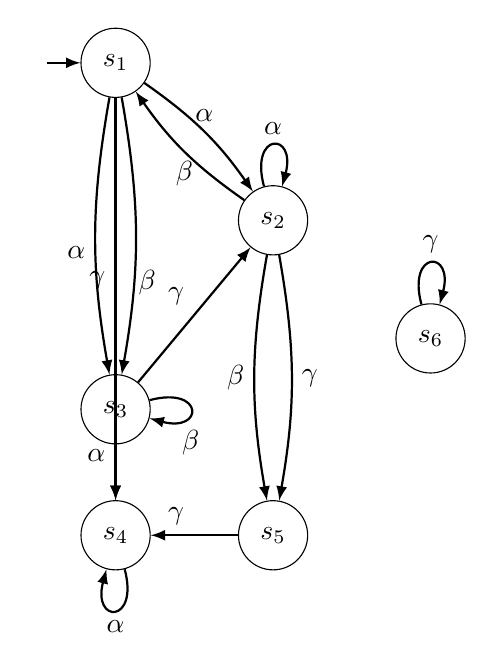
\begin{tikzpicture} [scale=2, every initial by arrow/.style={thick}]
		

		\path
		(\basex,		\basey) 		node[state,init] (s1) 	{$\state_1$} 
		(\basex+2,		\basey+0) 		node[state] (s2) 	{$\state_2$} 
		(\basex+1,		\basey-1.2) 	node[state] (s3) 	{$\state_3$} 
		(\basex,		\basey-2) 		node[state] (s4) 	{$\state_4$} 
		(\basex+2,		\basey-2) 		node[state] (s5) 	{$\state_5$}
		(\basex+3,		\basey-.75) 	node[state] (s6) 	{$\state_6$}
				
		;
		
%		
		\path [bendtrans] 	(s1) 	edge node [midway,above]				{\action} 		(s2);
		\path [bendtrans] 	(s1) 	edge node [near end,above right=-2pt]	{\actionb} 		(s3);
		\path [bendtransr] 	(s1) 	edge node [midway,below left]	{\action} 		(s3);
		\path [trans] 		(s1) 	edge node [midway,above left]	{\actionc} 		(s4);
		\path [bendtrans] 	(s2) 	edge node [midway,below]		{\actionb} 		(s1);
		\path [bendtransr] 	(s2) 	edge node [midway,left]			{\actionb} 		(s5);
		\path [bendtrans] 	(s2) 	edge node [midway,right]		{\actionc} 		(s5);
		\path [trans] 		(s3)	edge node [midway,above left]	{\actionc} 		(s2);
		\path [trans] 		(s3)	edge node [midway,above left]	{\action} 		(s4);
		\path [trans] 		(s5)	edge node [midway,above left]	{\actionc} 		(s4);
		
		\path [trans] 		(s2) 	edge [loop above] node [midway,above] {\action} 	(s2);
		\path [trans] 		(s3) 	edge [loop right] node [midway,below=4pt] {\actionb} 	(s3);
		\path [trans] 		(s4) 	edge [loop below] node [midway,below] {\action} 	(s4);
		\path [trans] 		(s6) 	edge [loop above] node [midway,above] {\actionc} 	(s6);
		
		
		%		midway, at start, near start, very near start, at end, near end, very near end
		
		
	\end{tikzpicture}
\end{document}
	\end{minipage}%
	\begin{minipage}{.5\textwidth}
		\hspace{5mm}
		\documentclass[tikz,preview]{standalone}
%\usepackage{prelude}

%%%%%%%%%%%%%%%%%%%%%%%%%%%%%%%%%%%% PACKAGES %%%%%%%%%%%%%%%%%%%%%%%%%%%%%%%%%%%%%%%%%%

\usepackage{inputenc,fontenc}
\usepackage[a4paper,margin=3cm]{geometry}
\usepackage[english]{babel}
%\usepackage[german]{babel}
%\usepackage[fixlanguage]{babelbib}


\usepackage{bbold}
\usepackage{amsthm}
\usepackage{amsmath}
\usepackage{amssymb} % doteqdot
\usepackage[dvipsnames]{xcolor}
\usepackage{standalone}
\usepackage{tikz}[mode=buildnew]
\usepackage{cite}
\usepackage{xspace}
\usepackage{relsize}
\usepackage{mathtools} % mathclap
%\usepackage{MnSymbol}
\usepackage{hyperref}
\usepackage{url}
\usepackage{listings} % for code
\usepackage[T1]{fontenc} %<
\hypersetup{
	colorlinks,
	citecolor=black,
	filecolor=black,
	linkcolor=black,
	urlcolor=black
}
\usepackage{pgfplots}
\pgfplotsset{compat=1.18}
%\usepackage{courier} %% Sets font for listing as Courier. But also for url and texttt!
\usepackage{listings, xcolor}
\usepackage{graphicx}
\usepackage{subcaption}

\usetikzlibrary{calc}
%\usepackage{xparse} % \newDocumentCommand for multiple optional arguments
%\usepackage{titlecaps}



%%%%%%%%%%%%%%%%%%%%%%%%%%%%%%%%%%%% THEOREMSTYLES %%%%%%%%%%%%%%%%%%%%%%%%%%%%%%%%%%

\theoremstyle{definition}
\newtheorem{definition}{Definition}[section]
\newtheorem{exmp}{Beispiel}[section]
%\AfterEndEnvironment{definition}{\noindent\ignorespaces}

\theoremstyle{theorem}
\newtheorem{theorem}{Satz}[section]
\newtheorem{proposition}{Proposition}[section]
%\AfterEndEnvironment{theorem}{\noindent\ignorespaces}

\theoremstyle{korollary}
\newtheorem{korollary}{Korollar}[section]
%\AfterEndEnvironment{korollary}{\noindent\ignorespaces}


\tikzset{
	mstate/.style={draw, circle, minimum size=.94cm}, 
	gstate/.style={draw, rectangle, minimum size=.8cm},
	varstate/.style={draw,rectangle, rounded corners, minimum size=1}, 
	trans/.style={draw, ->, thick},
	bendtrans/.style={draw, ->, thick, bend left=10},
	bendtransr/.style={draw, ->, thick, bend right=10},
	init/.style={initial, initial distance=6pt, initial text=},
	every loop/.style={min distance=5pt, looseness=8},
	>=latex
}
\usetikzlibrary{automata,positioning}

%auto shift/.style={auto=right,->,
%	to path={ let \p1=(\tikztostart),\p2=(\tikztotarget),
%		\n1={atan2(\y2-\y1,\x2-\x1)},\n2={\n1+180}
%		in ($(\tikztostart.{\n1})!1mm!270:(\tikztotarget.{\n2})$) -- 
%		($(\tikztotarget.{\n2})!1mm!90:(\tikztostart.{\n1})$) \tikztonodes}},

%%%%%%%%%%%%%%%%%%%%%%%%%%%%%%%%%%% MY MACROS %%%%%%%%%%%%%%%%%%%%%%%%%%%%%%%%%%%%%%%%%
%formatting
\newcommand{\comment}[2]{{\color{#1}#2}}
\newcommand{\redcomment}[1]{{\color{red}#1}}
\newcommand{\purpcomment}[1]{{\color{pink}#1}}
\newcommand{\bluecomment}[1]{{\color{blue}#1}}
\newcommand{\mt}[1]{\ensuremath{{#1}}\xspace}
\newcommand{\mynewcommand}[2]{\newcommand{#1}{\mt{#2}}} %% currently not used becaue of ide highlighting
\newcommand{\arr}{\mt{\to}}

%model checking terms
\newcommand{\mimicrel}{\mt{\mathcal{R}}}
\newcommand{\bisimeq}{\mt{\;\!\sim\;\!}}
\newcommand{\simorder}{\mt{\;\!\preceq\;\!}}
\newcommand{\simequiv}{\mt{\;\!\simeq\;\!}} %command already defined
\newcommand{\relts}{\mt{\;\!\bullet_{_{\tiny{TS}}}\;\!}}
\newcommand{\rel}{\mt{\;\!\bullet\;\!}}

%own names
\newcommand{\nm}[1]{#1\xspace}
\newcommand{\mdpN}{\nm{MDP}}
\newcommand{\mdpsN}{\nm{MDPs}}
\newcommand{\viewN}{\nm{view}}
\newcommand{\viewNC}{\nm{View}}
\newcommand{\viewsN}{\nm{views}}
\newcommand{\viewsNC}{\nm{Views}}
\newcommand{\grpfctsubN}{\nm{detached grouping function}}
\newcommand{\grpfctsubNC}{\nm{detached grouping function}}
\newcommand{\grpfctsubNCC}{\nm{Detached Grouping Function}}
\newcommand{\grpfctN}{\nm{grouping function}}
\newcommand{\grpfctNC}{\nm{Grouping function}}
\newcommand{\grpfctNCC}{\nm{Grouping Function}}
\newcommand{\grpfctsN}{\nm{grouping functions}}
\newcommand{\grpfctsNC}{\nm{Grouping functions}}
\newcommand{\grpfctsNCC}{\nm{Grouping Functions}}
\newcommand{\stmimicN}{\nm{state-mimic}}
\newcommand{\stmimicsN}{\nm{state-mimics}}
\newcommand{\stmimickingN}{\nm{state-mimicking}}
\newcommand{\stmimickedN}{\nm{state-mimicked}}
%\newcommand{\chosenphtypeNCC}{\nm{Transition System}}
%\newcommand{\chgphNC}{\nm{Transition system}}
%\newcommand{\chgphN}{\nm{transition system}}
%\newcommand{\chgphsNCC}{\nm{Transition Systems}}
%\newcommand{\chgphsNC}{\nm{Transition systems}}
%\newcommand{\chgphsN}{\nm{transition systems}}
\newcommand{\chgphNCC}{\nm{MDP}}
\newcommand{\chgphNC}{\nm{MDP}}
\newcommand{\chgphN}{\nm{MDP}}
\newcommand{\achgphN}{\nm{an MDP}}
\newcommand{\chgphsNCC}{\nm{MDPs}}
\newcommand{\chgphsNC}{\nm{MDPs}}
\newcommand{\chgphsN}{\nm{MDPs}}
\newcommand{\parllcompN}{\nm{parallel composition}}
\newcommand{\parllcompNC}{\nm{Parallel composition}}
\newcommand{\parllcompNCC}{\nm{Parallel Composition}}
\newcommand{\parllcompsN}{\nm{parallel compositions}}
\newcommand{\parllcompsNC}{\nm{Parallel compositions}}
\newcommand{\parllcompsNCC}{\nm{Parallel Compositions}}
\newcommand{\sccN}{\nm{SCC}}
\newcommand{\sccsN}{\nm{SCCs}}
\newcommand{\bsccN}{\nm{BSCC}}
\newcommand{\bsccsN}{\nm{BSCCs}}
\newcommand{\jgrapht}{\nm{jGraphtT}}

\newcommand{\outactident}{\nm{OutActionsIdent}}

%names
\newcommand{\iffN}{\nm{if and only if}}
\newcommand{\tsN}{\nm{TS}}

%% outactions identical
\newcommand{\outactidentstrong}{\nm{strong}}
\newcommand{\outactidentweak}{\nm{weak}}

% CORE DEFINITIONS
\newcommand{\grpfct}[1][\viewppty]{\mt{F_{#1}}}
\newcommand{\grpfctsub}[1][\viewppty]{\mt{\tilde{F}_{#1}}}
%\newcommand{\grpfctimg}[1]{\mt{{\grpfct}[{#1}]}}
%\newcommand{\fctimg}[2]{\mt{{#1}[{#2}]}}
\newcommand{\eqrelview}{\mt{R}}
\newcommand{\eqclassv}[1][\state]{\mt{\eqclass{#1}{\eqrelview}}}
\newcommand{\eqclasssetv}[1][\states]{\mt{{#1}/\eqrelview}} %OLD: \bigcup_{\state \in \states} \eqclassv
\newcommand{\viewid}{\mt{\mdp}}
\newcommand{\view}[1][\viewppty]{\mt{\viewid_{#1}}}
\newcommand{\imggrp}{\mt{\arbset}}
\newcommand{\imggrpsub}{\mt{X}}
\newcommand{\viewppty}{\mt{\theta}}
\newcommand{\pll}{\mt{\;\!\pllpure\;\!}}
\newcommand{\pllrev}{\mt{\pllpure^{-1}}}
\newcommand{\pllpure}{\mt{||}}
\newcommand{\compselectset}{\mt{Z}}
\newcommand{\compselectpure}{\mt{\pllpure_\compselectset}}
\newcommand{\compselect}{\mt{\;\pllpure_\compselectset\;}}
\newcommand{\remstates}{\mt{\bigcup_{\state \in \states \setminus \states_1}\{\{\state\}\}}}
\newcommand{\nogroupstates}[1][\states_2]{\mt{\bigcup_{\state \in \states \setminus {#1}}\{\{\state\}\}}}
\newcommand{\remelem}{\mt{\bullet}}
\newcommand{\nogroupset}{\mt{\xi}}
\newcommand{\remset}{\mt{\{\remelem\}}}
\newcommand{\gfctpll}{\mt{\grpfct[\pll]}}
\newcommand{\group}{\mt{\top}}
\newcommand{\imggrpbinview}{\mt{\{\remelem, \notppty\}}}
\newcommand{\viewappset}{\mt{\tilde{\states}}}
\newcommand{\hasppty}{\mt{\top}}
\newcommand{\notppty}{\mt{\bot}}
\newcommand{\disregardelem}{\mt{\Delta}}
\newcommand{\disregardelements}{\mt{{\disregardelem_1, \dots, \disregardelem_n}}}



%\newcommand{\mdp}{def}\mdp
%\newcommand{\mdpdef}



% EXAMPLE VIEWS
\newcommand{\pptyatomicprops}{\mt{\atomicprops}}
\newcommand{\pptyinitstates}{\mt{\initstates}}
\newcommand{\pptyinactsetsize}{\mt{|\inacts(\state)|}}
\newcommand{\pptyhasoutact}{\mt{\exists\outact}}
\newcommand{\pptyminoutact}[2]{\mt{#1\leq#2}}
\newcommand{\pptymaxoutact}[2]{\mt{#2\leq#1}}
\newcommand{\pptyspanoutact}[3]{\mt{#1\leq#2\leq#3}}
\newcommand{\pptyoutactsetsize}{\mt{|\outacts(\state)|}}
\newcommand{\pptyoutactsingle}{\mt{|\outacts(\state)|_1}}
\newcommand{\pptystrongoutactident}{\mt{\outacts(\state)_=}}
\newcommand{\pptyweakoutactident}{\mt{\outacts(\state)_\approx}}
\newcommand{\pptyhasinact}{\mt{\exists\inact}}
\newcommand{\pptymininact}[2]{\mt{#1\leq#2}}
\newcommand{\pptymaxinact}[2]{\mt{#2\leq#1}}
\newcommand{\pptyspaninact}[3]{\mt{#1\leq#2\leq#3}}
\newcommand{\pptyinactsingle}{\mt{|\inacts(\state)|_1}}
\newcommand{\pptystronginactident}{\mt{\inacts(\state)_=}}
\newcommand{\pptyweakinactident}{\mt{\inacts(\state)_\approx}}
\newcommand{\pptyparamvalueseq}{\mt{\var = \varval}}
\newcommand{\pptyparamvaluesneq}{\mt{\var \neq \varval}}
\newcommand{\pptyparamdnf}{\mt{VarDNF}}
\newcommand{\pptyparamcnf}{\mt{VarCNF}}
\newcommand{\pptyparamvalueseqopt}{\mt{\var = \varval}}
\newcommand{\pptyparamvalident}{\mt{Var:\varval}}
\newcommand{\pptydistance}{\mt{\distpath}}
\newcommand{\pptydistancerev}{\mt{\distpathrev}}
\newcommand{\pptydistancebi}{\mt{\distpathbi}}
\newcommand{\pptyhascycle}{\mt{\exists\cycle}}
\newcommand{\pptyexactactcycle}{\mt{\{\cycle_{\action,n}\}}}
\newcommand{\pptycycleset}{\mt{\cup{\{\state\}_\cycle}}}
\newcommand{\pptyexactcycle}{\mt{\{\cycle_n\}}}
\newcommand{\pptyscc}{\mt{scc}}
\newcommand{\pptybscc}{\mt{bscc}}
\newcommand{\pptyprop}{\mt{\redcomment{?}}}
\newcommand{\pptyident}{id}


\newcommand{\gfctatomicprops}{\mt{\grpfct[\pptyatomicprops]}}
\newcommand{\gfctinitstates}{\mt{\grpfct[\pptyinitstates]^\hasppty}}
\newcommand{\gfcthasoutaction}{\mt{\grpfct[\pptyhasoutact]^\hasppty}}
\newcommand{\gfctminoutaction}{\mt{\grpfct[\pptyminoutact{\numoutact}{\outact}]^\hasppty}}
\newcommand{\gfctmaxoutaction}{\mt{\grpfct[\pptymaxoutact{\numoutact}{\outact}]^\hasppty}}
\newcommand{\gfctspanoutaction}{\mt{\grpfct[\pptyspanoutact{\numoutactb}{\outact}{\numoutact}]^\hasppty}}
\newcommand{\gfctoutactsetsize}{\mt{\grpfct[\pptyoutactsetsize]}}
\newcommand{\gfctoutactsingle}{\mt{\grpfct[\pptyoutactsingle]^\notppty}}
\newcommand{\gfctstrongoutactident}{\mt{\grpfct[\pptystrongoutactident]}}
\newcommand{\gfctweakoutactident}{\mt{\grpfct[\pptyweakoutactident]}}
\newcommand{\gfcthasinaction}{\mt{\grpfct[\pptyhasinact]^\hasppty}}
\newcommand{\gfctmininaction}{\mt{\grpfct[\pptymininact{\numinact}{\inact}]^\hasppty}}
\newcommand{\gfctmaxinaction}{\mt{\grpfct[\pptymaxinact{\numinact}{\inact}]^\hasppty}}
\newcommand{\gfctspaninaction}{\mt{\grpfct[\pptyspaninact{\numinactb}{\inact}{\numinact}]^\hasppty}}
\newcommand{\gfctinactsetsize}{\mt{\grpfct[\pptyinactsetsize]}}
\newcommand{\gfctinactsingle}{\mt{\grpfct[\pptyinactsingle]^\notppty}}
\newcommand{\gfctstronginactident}{\mt{\grpfct[\pptystronginactident]}}
\newcommand{\gfctweakinactident}{\mt{\grpfct[\pptyweakinactident]}}
\newcommand{\gfctparamvalueseq}{\mt{\grpfct[\pptyparamvalueseq]^\hasppty}}
\newcommand{\gfctparamvaluesneq}{\mt{\grpfct[\pptyparamvaluesneq]^\hasppty}}
\newcommand{\gfctparamdnf}{\mt{\grpfct[\pptyparamdnf]^\hasppty}}
\newcommand{\gfctparamcnf}{\mt{\grpfct[\pptyparamcnf]^\hasppty}}
\newcommand{\gfctparamvalueseqopt}{\mt{\pptyparamvalueseqopt}}
\newcommand{\gfctparamvalident}{\mt{\grpfct[\pptyparamvalident]}}
\newcommand{\gfctdistance}{\mt{\grpfct[\pptydistance]}}
\newcommand{\gfctdistancerev}{\mt{\grpfct[\pptydistancerev]}}
\newcommand{\gfctdistancebi}{\mt{\grpfct[\pptydistancebi]}}
\newcommand{\gfcthascycle}{\mt{\grpfct[\pptyhascycle]}}
\newcommand{\gfctexactcycle}{\mt{\grpfct[\pptyexactcycle]}}
\newcommand{\gfctcycleset}{\mt{\grpfct[\pptycycleset]}}
\newcommand{\gfctexactactcycle}{\mt{\grpfct[\pptyexactactcycle]}}
\newcommand{\gfctscc}{\mt{\grpfct[\pptyscc]}}
\newcommand{\gfctbscc}{\mt{\grpfct[\pptybscc]}}
\newcommand{\gfctprop}{\mt{\grpfct[\pptyprop]}}
\newcommand{\gfctident}{\mt{\grpfct[\pptyident]}}

\newcommand{\gfctsubatomicprops}{\mt{\grpfctsub[\pptyatomicprops]}}
\newcommand{\gfctsubinitstates}{\mt{\grpfctsub[\pptyinitstates]^\hasppty}}
\newcommand{\gfctsubhasoutaction}{\mt{\grpfctsub[\pptyhasoutact]^\hasppty}}
\newcommand{\gfctsubminoutaction}{\mt{\grpfctsub[\pptyminoutact{\numoutact}{\outact}]^\hasppty}}
\newcommand{\gfctsubmaxoutaction}{\mt{\grpfctsub[\pptymaxoutact{\numoutact}{\outact}]^\hasppty}}
\newcommand{\gfctsubspanoutaction}{\mt{\grpfctsub[\pptyspanoutact{\numoutactb}{\outact}{\numoutact}]^\hasppty}}
\newcommand{\gfctsuboutactsetsize}{\mt{\grpfctsub[\pptyoutactsetsize]}}
\newcommand{\gfctsuboutactsingle}{\mt{\grpfctsub[\pptyoutactsingle]^\notppty}}
\newcommand{\gfctsubstrongoutactident}{\mt{\grpfctsub[\pptystrongoutactident]^\hasppty}}
\newcommand{\gfctsubweakoutactident}{\mt{\grpfctsub[\pptyweakoutactident]^\hasppty}}
\newcommand{\gfctsubhasinaction}{\mt{\grpfctsub[\pptyhasinact]}}
\newcommand{\gfctsubmininaction}{\mt{\grpfctsub[\pptymininact{\numinact}{\inact}]}}
\newcommand{\gfctsubmaxinaction}{\mt{\grpfctsub[\pptymaxinact{\numinact}{\inact}]}}
\newcommand{\gfctsubspaninaction}{\mt{\grpfctsub[\pptyspaninact{\numinactb}{\inact}{\numinact}]}}
\newcommand{\gfctsubinactsetsize}{\mt{\grpfctsub[\pptyinactsetsize]^\hasppty}}
\newcommand{\gfctsubinactsingle}{\mt{\grpfctsub[\pptyinactsingle]^\notppty}}
\newcommand{\gfctsubstronginactident}{\mt{\grpfctsub[\pptystronginactident]}}
\newcommand{\gfctsubweakinactident}{\mt{\grpfctsub[\pptyweakinactident]}}
\newcommand{\gfctsubparamvalueseq}{\mt{\grpfctsub[\pptyparamvalueseq]^\hasppty}}
\newcommand{\gfctsubparamvaluesneq}{\mt{\grpfctsub[\pptyparamvaluesneq]^\hasppty}}
\newcommand{\gfctsubparamdnf}{\mt{\grpfctsub[\pptyparamdnf]^\hasppty}}
\newcommand{\gfctsubparamcnf}{\mt{\grpfctsub[\pptyparamcnf]^\hasppty}}
\newcommand{\gfctsubparamvalueseqopt}{\mt{\pptyparamvalueseqopt}}
\newcommand{\gfctsubparamvalident}{\mt{\grpfctsub[\pptyparamvalident]}}
\newcommand{\gfctsubdistance}{\mt{\grpfctsub[\pptydistance]}}
\newcommand{\gfctsubdistancerev}{\mt{\grpfctsub[\pptydistancerev]}}
\newcommand{\gfctsubdistancebi}{\mt{\grpfctsub[\pptydistancebi]}}
\newcommand{\gfctsubhascycle}{\mt{\grpfctsub[\pptyhascycle]^\hasppty}}
\newcommand{\gfctsubexactcycle}{\mt{\grpfctsub[\pptyexactcycle]}}
\newcommand{\gfctsubcycleset}{\mt{\grpfctsub[\pptycycleset]}}
\newcommand{\gfctsubexactactcycle}{\mt{\grpfctsub[\pptyexactactcycle]}}
\newcommand{\gfctsubscc}{\mt{\grpfctsub[\pptyscc]}}
\newcommand{\gfctsubbscc}{\mt{\grpfctsub[\pptybscc]}}
\newcommand{\gfctsubprop}{\mt{\grpfctsub[\pptyprop]}}
\newcommand{\gfctsubident}{\mt{\grpfctsub[\pptyident]}}


\newcommand{\viewatomicprops}{\mt{\view[\pptyatomicprops]}}
\newcommand{\viewinitstates}{\mt{\view[\pptyinitstates]^\hasppty}}
\newcommand{\viewhasoutaction}{\mt{\view[\pptyhasoutact]^\hasppty}}
\newcommand{\viewminoutaction}{\mt{\view[\pptyminoutact{\numoutact}{\outact}]^\hasppty}}
\newcommand{\viewmaxoutaction}{\mt{\view[\pptymaxoutact{\numoutact}{\outact}]^\hasppty}}
\newcommand{\viewspanoutaction}{\mt{\view[\pptyspanoutact{\numoutactb}{\outact}{\numoutact}]^\hasppty}}
\newcommand{\viewoutactsetsize}{\mt{\view[\pptyoutactsetsize]}}
\newcommand{\viewoutactsingle}{\mt{\view[\pptyoutactsingle]^\notppty}}
\newcommand{\viewstrongoutactident}{\mt{\view[\pptystrongoutactident]}}
\newcommand{\viewweakoutactident}{\mt{\view[\pptyweakoutactident]}}
\newcommand{\viewhasinaction}{\mt{\view[\pptyhasinact]^\hasppty}}
\newcommand{\viewmininaction}{\mt{\view[\pptymininact{\numinact}{\inact}]^\hasppty}}
\newcommand{\viewmaxinaction}{\mt{\view[\pptymaxinact{\numinact}{\inact}]^\hasppty}}
\newcommand{\viewspaninaction}{\mt{\view[\pptyspaninact{\numinactb}{\inact}{\numinact}]^\hasppty}}
\newcommand{\viewinactsetsize}{\mt{\view[\pptyinactsetsize]}}
\newcommand{\viewinactsingle}{\mt{\view[\pptyinactsingle]^\notppty}}
\newcommand{\viewstronginactident}{\mt{\view[\pptystronginactident]}}
\newcommand{\viewweakinactident}{\mt{\view[\pptyweakinactident]}}
\newcommand{\viewparamvalueseq}{\mt{\view[\pptyparamvalueseq]}}
\newcommand{\viewparamvaluesneq}{\mt{\view[\pptyparamvaluesneq]}}
\newcommand{\viewparamdnf}{\mt{\view[\pptyparamdnf]^\hasppty}}
\newcommand{\viewparamcnf}{\mt{\view[\pptyparamcnf]^\hasppty}}
\newcommand{\viewparamvalueseqopt}{\mt{\pptyparamvalueseqopt}}
\newcommand{\viewparamvalident}{\mt{\view[\pptyparamvalident]}}
\newcommand{\viewdistance}{\mt{\view[\pptydistance]}}
\newcommand{\viewdistancerev}{\mt{\view[\pptydistancerev]}}
\newcommand{\viewdistancebi}{\mt{\view[\pptydistancebi]}}
\newcommand{\viewhascycle}{\mt{\view[\pptyhascycle]}}
\newcommand{\viewexactcycle}{\mt{\view[\pptyexactcycle]}}
\newcommand{\viewcycleset}{\mt{\view[\pptycycleset]}}
\newcommand{\viewexactactcycle}{\mt{\view[\pptyexactactcycle]}}
\newcommand{\viewscc}{\mt{\view[\pptyscc]}}
\newcommand{\viewbscc}{\mt{\view[\pptybscc]}}
\newcommand{\viewprop}{\mt{\view[\pptyprop]}}
\newcommand{\viewident}{\mt{\view[\pptyident]}}

%\newcommand{\viewatomicprops}{\mt{\view[\atomicprops]}}
%\newcommand{\viewinitstates}{\mt{\view[\initstates]}}
%\newcommand{\viewhasoutaction}{\mt{\view[\pptyhasoutact]}}
%\newcommand{\viewminoutaction}{\mt{\view[\pptyminoutact{\numoutact}{\outact}]}}
%\newcommand{\viewmaxoutaction}{\mt{\view[\pptymaxoutact{\numoutact}{\outact}]}}
%\newcommand{\viewspanoutaction}{\mt{\view[\pptyspanoutact{\numoutactb}{\outact}{\numoutact}]}}
%\newcommand{\viewoutactsetsize}{\mt{\view[\pptyoutactsetsize]}}
%\newcommand{\viewoutactsingle}{\mt{\view[\pptyoutactsingle]}}
%\newcommand{\viewstrongoutactident}{\mt{\view[\outacts(\state)_=]}}
%\newcommand{\viewweakoutactident}{\mt{\view[\outacts(\state)_\approx]}}
%\newcommand{\viewhasinaction}{\mt{\view[\pptyhasinact]}}
%\newcommand{\viewmininaction}{\mt{\view[\pptymininact{\numinact}{\inact}]}}
%\newcommand{\viewmaxinaction}{\mt{\view[\pptymaxinact{\numinact}{\inact}]}}
%\newcommand{\viewspaninaction}{\mt{\view[\pptyspaninact{\numinactb}{\inact}{\numinact}]}}
%\newcommand{\viewinactsetsize}{\mt{\view[\pptyinactsetsize]}}
%\newcommand{\viewinactsingle}{\mt{\view[\pptyinactsingle]}}
%\newcommand{\viewstronginactident}{\mt{\view[\inacts(\state)_=]}}
%\newcommand{\viewweakinactident}{\mt{\view[\inacts(\state)_\approx]}}
%\newcommand{\viewparamvalueseq}{\mt{\view[\var = \varval]}}
%\newcommand{\viewparamvaluesneq}{\mt{\view[\var \neq \varval]}}
%\newcommand{\viewparamdnf}{\mt{\view[VarDNF]}}
%\newcommand{\viewparamcnf}{\mt{\view[VarCNF]}}
%\newcommand{\viewparamvalident}{\mt{\view[\pptyparamvalident]}}
%\newcommand{\viewdistance}{\mt{\view[\pptydistance]}}
%\newcommand{\viewhascycle}{\mt{\view[\exists\cycle]}}
%\newcommand{\viewexactcycle}{\mt{\view[\pptyexactcycle]}}
%\newcommand{\viewcycleset}{\mt{\view[\pptycycleset]}}
%\newcommand{\viewexactactcycle}{\mt{\view[\pptyexactactcycle]}}
%\newcommand{\viewscc}{\mt{\view[scc]}}
%\newcommand{\viewbscc}{\mt{\view[bscc]}}

%actions
\newcommand{\numoutact}{\mt{n}}
\newcommand{\numoutactb}{\mt{m}}
\newcommand{\numinact}{\mt{n}}
\newcommand{\numinactb}{\mt{m}}

\newcommand{\predmaxoutact}[1][\numoutact]{\mt{Q_{\outact\leq#1}(\state,\state_1, \dots, \state_{#1+1})}}
\newcommand{\predminoutact}[1][\numoutact]{\mt{Q_{#1\leq\outact}(\state,\state_1, \dots, \state_{#1})}}
\newcommand{\formoutact}[1][\state]{\mt{C_{#1,\outact}}}
\newcommand{\predmaxinact}[1][\numinact]{\mt{Q_{\inact\leq#1}(\state,\state_1, \dots, \state_{#1+1})}}
\newcommand{\predmininact}[1][\numinact]{\mt{Q_{#1\leq\inact}(\state,\state_1, \dots, \state_{#1})}}

\newcommand{\outact}[1][\action]{\mt{\overrightarrow{#1}}}
\newcommand{\outacts}{\mt{\overrightarrow{\actions}}}
\newcommand{\inact}{\mt{\overleftarrow{\action}}}
\newcommand{\inacts}[1][\action]{\mt{\overleftarrow{#1}}}

%%Parameters
\newcommand{\vars}[1][\mdp]{\mt{V\!ar_{#1}}}
\newcommand{\var}{\mt{x}}
\newcommand{\varstate}[1][]{\mt{\var_{\state#1}}}
\newcommand{\varval}{\mt{a}}
\newcommand{\vareval}[1][\mdp]{\mt{V\!arEval_{#1}}}
\newcommand{\varevalimg}[1][\mdp]{\mt{\vareval[#1][\states,\vars]}}
\newcommand{\varevalimgset}{\mt{\arbset}}
\newcommand{\someparam}{\mt{\tilde{x}}}
\newcommand{\eqorneq}{\mt{\;\doteqdot\;}}
\newcommand{\varstyle}[2]{\mt{\langle#1,#2\rangle}}




%\makeatletter
%\newcommand{\overleftrightsmallarrow}{\mathpalette{\overarrowsmall@\leftrightarrowfill@}}
%\newcommand{\overrightsmallarrow}{\mathpalette{\overarrowsmall@\rightarrowfill@}}
%\newcommand{\overleftsmallarrow}{\mathpalette{\overarrowsmall@\leftarrowfill@}}
%\newcommand{\overarrowsmall@}[3]{%
%	\vbox{%
%		\ialign{%
%			##\crcr
%			#1{\smaller@style{#2}}\crcr
%			\noalign{\nointerlineskip}%
%			$\m@th\hfil#2#3\hfil$\crcr
%		}%
%	}%
%}
%\def\smaller@style#1{%
%	\ifx#1\displaystyle\scriptstyle\else
%	\ifx#1\textstyle\scriptstyle\else
%	\scriptscriptstyle
%	\fi
%	\fi
%}
%\makeatother
%\newcommand{\te}[1]{\overleftrightsmallarrow{#1}}

% Distance
\newcommand{\fctdist}{\mt{distance}}
\newcommand{\fctdistdefault}{\mt{\fctdist(\chgph, \smstates, \grandist)}}
\newcommand{\distval}{\mt{d}}
\newcommand{\grandist}{\mt{n}}
\let\path\oldpath
\newcommand{\path}{\mt{P}}
\newcommand{\pathbi}{\mt{\bar{\path}}}
\newcommand{\pathsecfull}{\mt{(\state_0, \action_0, \state_1, \action_1, \dots, \action_{n}, \state_{n+1})}}
\newcommand{\lenpath}{\mt{len}}
\newcommand{\pfirst}{\mt{first}}
\newcommand{\plast}{\mt{last}}
\newcommand{\pathset}{\mt{\path_\chgph}}
\newcommand{\pathbiset}{\mt{\pathbi_\chgph}}
\newcommand{\distpath}{\mt{\overrightarrow{dist}}}
\newcommand{\distpathrev}{\mt{\overleftarrow{dist}}}
\newcommand{\distpathbi}{\mt{\overline{dist}}}
%Cycles
\newcommand{\cyclesecfull}{\mt{(\state_0, \action_0, \state_1, \action_1, \dots, \action_{n-1}, \state_0)}}
\newcommand{\fctfindcycles}{\mt{findCycles}}
\newcommand{\cycle}{\mt{C}}
\newcommand{\cycleset}{\mt{\cycle_{\mdp, n}}}
\newcommand{\lencycle}{\mt{len}}
% strongly connected components
\newcommand{\scc}{\mt{T}}
\newcommand{\setscc}{\mt{SCC_{\chgph,n}}}
\newcommand{\setbscc}{\mt{BSCC_{\chgph,n}}}

% properties
\newcommand{\propfct}{\mt{f}}

% all Systems
\newcommand{\chgph}{\mt{\mdp}}
\newcommand{\chgphtuple}{\mt{\mdptuple}}
\newcommand{\chgphtupledist}{\mt{\mdptupledist}}

\newcommand{\states}{\mt{S}}
\newcommand{\actions}{\mt{Act}}
\newcommand{\atomicprops}{\mt{AP}}
\newcommand{\labelingfct}{\mt{L}}
\newcommand{\init}{\mt{\initdistrib}} % use MDP % refers to the underlying set
\newcommand{\trans}{\mt{\probtfunc}} % use MDP % refers to the underlying set
\newcommand{\smstates}{\mt{\tilde{\states}}}


\newcommand{\state}{\mt{s}}
\newcommand{\action}{\mt{\alpha}}
\newcommand{\actionb}{\mt{\beta}}
\newcommand{\actionc}{\mt{\gamma}}
\newcommand{\smstate}{\mt{\tilde{\state}}}



% transition sysstems
\newcommand{\ts}{\mt{TS}}
\newcommand{\transitionrel}{\mt{\longrightarrow}}
\newcommand{\initstates}{\mt{I}}
\newcommand{\transitionsystem}{\mt
	{(\states, \actions, \transitionrel, \initstates, \atomicprops, \labelingfct)}
}
\newcommand{\tstupledist}{\mt{(\states', \actions',\transitionrel', \initstates', \labelingfct')}}


%Markov chains and MDP
\newcommand{\mdp}{\mt{\autm}}
\newcommand{\mdptuple}{\mt{(\states, \actions, \probtfunc, \initdistrib, \atomicprops, \labelingfct)}}
\newcommand{\mdptupledist}{\mt{(\states', \actions', \probtfunc', \initdistrib', \atomicprops', \labelingfct')}}
\newcommand{\autm}{\mt{\mathcal{M}}}
\newcommand{\probtfunc}{\mt{\textbf{P}}}
\newcommand{\initdistrib}{\mt{\iota_{init}}}


%maths
\newcommand{\powerset}[1]{\mt{\mathcal{P}(#1)}}
\newcommand{\eqclass}[2]{\mt{[#1]_{#2}}}%{\mt{#1 / #2}}
\newcommand{\impr}{\mt{\hspace{3mm}\Rightarrow\hspace{2mm}}}
\newcommand{\impl}{\mt{\hspace{3mm}\Leftarrow\hspace{2mm}}}
\newcommand{\natnums}{\mt{\mathbb{N}}} 
\newcommand{\realnums}{\mt{\mathbb{R}}}
\newcommand{\intmodn}[1][n]{\mt{\mathbb{Z}_{#1}}}
\newcommand{\arbset}{\mt{M}}
\newcommand{\bigsum}[2][]{\mt{\mathlarger{\sum}_{#2}^{#1}}}
\newcommand{\bbigsum}[2][]{\mt{\mathlarger{\mathlarger{\sum}}_{#2}^{#1}}}
\newcommand{\invimage}[2]{#1^{\mt{-1}(#2)}}
\newcommand{\img}{\mt{Img}}
\newcommand{\cond}{\mt{\,|\,}}

%tickz
%% \definecolor{darkred}{RGB}{196, 42, 42}

%implementation
\newcommand{\pmcvis}{\nm{PMC-Vis}}





\begin{document}
	\newcommand{\basex}{0}
	\newcommand{\basey}{0}
	\newcommand{\createstate}[3]{\node[draw, circle, minimum size=1cm] (#1) at (#2) {#3}}
	
	
	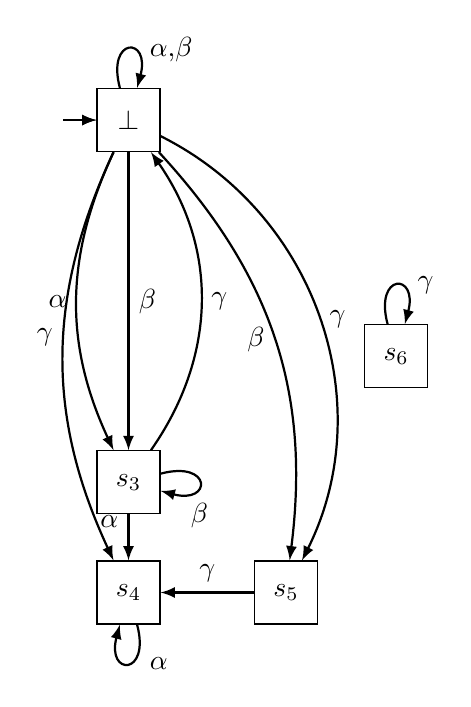
\begin{tikzpicture} [scale=2, every initial by arrow/.style={thick}]
		

	\path
	(\basex+1,		\basey) 		node[gstate,init, initial left] (sbot) 	{$\notppty$} 
	(\basex+1,		\basey-1.3) 	node[gstate] (s3) 	{$\state_3$} 
	(\basex,		\basey-2) 		node[gstate] (s4) 	{$\state_4$} 
	(\basex+2,		\basey-2)		node[gstate] (s5) 	{$\state_5$} 
	(\basex+2.7,	\basey-.5) 		node[gstate] (s6) 	{$\state_6$}

	;

	\path [trans, bend right=25] 		(sbot) 	edge node [midway,above left]		{\actionc} 		(s4);
	\path [trans] 		(sbot) 	edge node [midway,right]			{\actionb} 		(s3);
	\path [trans, bend right=25] 		(sbot) 	edge node [midway,left]				{\action} 		(s3);
	\path [trans, bend left=25](sbot) 	edge node [midway,left]			{\actionb} 		(s5);
	\path [trans, bend left=45] (sbot) 	edge node [midway,right]		{\actionc} 		(s5);
	\path [trans,bend right=35] 	(s3) 	edge node [midway,right]	{\actionc} 		(sbot);
	\path [trans] 	(s3) 	edge node [midway,above left]	{\action} 		(s4);
	\path [trans] 	(s5) 	edge node [midway,above]	{\actionc} 		(s4);
	
%	\path [trans] 		(sbot) 	edge [loop, in=15, out=50, looseness=6] node [midway,right] {\action,\actionb} 	(sbot);
	\path [trans] 		(sbot) 	edge [loop above] node [midway,right=4pt] {\action,\actionb} 	(sot);
	\path [trans] 		(s3) 	edge [loop right] node [midway,below=4pt] {\actionb} 	(s3);
	\path [trans] 		(s4) 	edge [loop below] node [midway,right=4pt] {\action} 	(s4);
	\path [trans] 		(s6) 	edge [loop above] node [midway,right=4pt] {\actionc} 	(s6);
	
	
	%		midway, at start, near start, very near start, at end, near end, very near end
		
		
	\end{tikzpicture}
\end{document}
	\end{minipage}
	\caption{Simplified representations of \mdp (left) and the \viewN $\view[\pptymaxoutact{1}{\outact}]$ on it (right)}
	\label{fig:outActMaxAfter} 
\end{figure}

We already know that for a given $\state \in \states$ the expressions $\exists \state_1, \dots, \state_\numoutact \in \states: \predminoutact$ and $\forall \state_1, \dots, \state_{\numoutactb+1} \in \states: \predmaxoutact[\numoutactb]$ from Definition \ref{def:minoutaction} and Definition \ref{def:viewmaxoutaction} require that \state has minimal and maximal amount of outgoing transitions with an action \action respectively. Hence the conjunction will be true for states where the amount of outgoing transitions with action \action is element of the set $\{\numoutactb, \numoutact+1, \dots, \numoutact-1, \numoutact\}$. We will write for this that the number of outgoing actions is \emph{in the span}.

For a given state \state and action \action we set
\[
\formoutact:= \exists \state_1, \dots, \state_\numoutactb \in \states: \predminoutact[\numoutactb]\land \\
\forall \state_1, \dots, \state_{\numoutact+1} \in \states: \predmaxoutact
\]

for convenience. \formoutact is true  \iffN the number of outgoing actions is in the span. For $\state_1, \state_2 \in \states$ it is $\gfctspanoutaction(\state_1) = \gfctspanoutaction(\state_2)$ \iffN $\formoutact[\state_1] \land \formoutact[\state_2]$ or $\state_1 = \state_2$. Then its equivalence classes are

\begin{align*}
	\eqclassv &= \{\state \in \states \mid \gfctspanoutaction(\state) = \action\} &\formoutact \text{ true} \\
	\eqclassv &= \{\state \in \states \mid \gfctspanoutaction(\state) = \state\} = \{\state\} &\text{ otherwise}	
\end{align*}

The new set of states $\states'$ of the view \viewspanoutaction is the union of the equivalence classes of equivalence relation \eqrelview on the set of states \states of the original \chgphN. Hence it is $\states' = \bigcup_{\state \in \states} \eqclassv =: \states_1 \cup \states_2$ where

\begin{align*}
	\states_1 &:= \{\state \in \states \mid \gfctspanoutaction(\state) = \action\} \\
	&\hspace{1.15mm}= \{\state \in \states  \mid \formoutact \text{ true}\} \\
	&\hspace{1.15mm}= \{\state \in \states \mid \text{the action } \action \text{ is outgoing } \numoutactb \text{ to } \numoutact \text{ times}\} \text{ and} \\
	\states_2 &:= \remstates.
\end{align*}

\begin{figure}[h]
	\begin{minipage}{.5\textwidth}
		\hspace{5mm}
		\documentclass[tikz,preview]{standalone}
%\usepackage{prelude}

%%%%%%%%%%%%%%%%%%%%%%%%%%%%%%%%%%%% PACKAGES %%%%%%%%%%%%%%%%%%%%%%%%%%%%%%%%%%%%%%%%%%

\usepackage{inputenc,fontenc}
\usepackage[a4paper,margin=3cm]{geometry}
\usepackage[english]{babel}
%\usepackage[german]{babel}
%\usepackage[fixlanguage]{babelbib}


\usepackage{bbold}
\usepackage{amsthm}
\usepackage{amsmath}
\usepackage{amssymb} % doteqdot
\usepackage[dvipsnames]{xcolor}
\usepackage{standalone}
\usepackage{tikz}[mode=buildnew]
\usepackage{cite}
\usepackage{xspace}
\usepackage{relsize}
\usepackage{mathtools} % mathclap
%\usepackage{MnSymbol}
\usepackage{hyperref}
\usepackage{url}
\usepackage{listings} % for code
\usepackage[T1]{fontenc} %<
\hypersetup{
	colorlinks,
	citecolor=black,
	filecolor=black,
	linkcolor=black,
	urlcolor=black
}
\usepackage{pgfplots}
\pgfplotsset{compat=1.18}
%\usepackage{courier} %% Sets font for listing as Courier. But also for url and texttt!
\usepackage{listings, xcolor}
\usepackage{graphicx}
\usepackage{subcaption}

\usetikzlibrary{calc}
%\usepackage{xparse} % \newDocumentCommand for multiple optional arguments
%\usepackage{titlecaps}



%%%%%%%%%%%%%%%%%%%%%%%%%%%%%%%%%%%% THEOREMSTYLES %%%%%%%%%%%%%%%%%%%%%%%%%%%%%%%%%%

\theoremstyle{definition}
\newtheorem{definition}{Definition}[section]
\newtheorem{exmp}{Beispiel}[section]
%\AfterEndEnvironment{definition}{\noindent\ignorespaces}

\theoremstyle{theorem}
\newtheorem{theorem}{Satz}[section]
\newtheorem{proposition}{Proposition}[section]
%\AfterEndEnvironment{theorem}{\noindent\ignorespaces}

\theoremstyle{korollary}
\newtheorem{korollary}{Korollar}[section]
%\AfterEndEnvironment{korollary}{\noindent\ignorespaces}


\tikzset{
	mstate/.style={draw, circle, minimum size=.94cm}, 
	gstate/.style={draw, rectangle, minimum size=.8cm},
	varstate/.style={draw,rectangle, rounded corners, minimum size=1}, 
	trans/.style={draw, ->, thick},
	bendtrans/.style={draw, ->, thick, bend left=10},
	bendtransr/.style={draw, ->, thick, bend right=10},
	init/.style={initial, initial distance=6pt, initial text=},
	every loop/.style={min distance=5pt, looseness=8},
	>=latex
}
\usetikzlibrary{automata,positioning}

%auto shift/.style={auto=right,->,
%	to path={ let \p1=(\tikztostart),\p2=(\tikztotarget),
%		\n1={atan2(\y2-\y1,\x2-\x1)},\n2={\n1+180}
%		in ($(\tikztostart.{\n1})!1mm!270:(\tikztotarget.{\n2})$) -- 
%		($(\tikztotarget.{\n2})!1mm!90:(\tikztostart.{\n1})$) \tikztonodes}},

%%%%%%%%%%%%%%%%%%%%%%%%%%%%%%%%%%% MY MACROS %%%%%%%%%%%%%%%%%%%%%%%%%%%%%%%%%%%%%%%%%
%formatting
\newcommand{\comment}[2]{{\color{#1}#2}}
\newcommand{\redcomment}[1]{{\color{red}#1}}
\newcommand{\purpcomment}[1]{{\color{pink}#1}}
\newcommand{\bluecomment}[1]{{\color{blue}#1}}
\newcommand{\mt}[1]{\ensuremath{{#1}}\xspace}
\newcommand{\mynewcommand}[2]{\newcommand{#1}{\mt{#2}}} %% currently not used becaue of ide highlighting
\newcommand{\arr}{\mt{\to}}

%model checking terms
\newcommand{\mimicrel}{\mt{\mathcal{R}}}
\newcommand{\bisimeq}{\mt{\;\!\sim\;\!}}
\newcommand{\simorder}{\mt{\;\!\preceq\;\!}}
\newcommand{\simequiv}{\mt{\;\!\simeq\;\!}} %command already defined
\newcommand{\relts}{\mt{\;\!\bullet_{_{\tiny{TS}}}\;\!}}
\newcommand{\rel}{\mt{\;\!\bullet\;\!}}

%own names
\newcommand{\nm}[1]{#1\xspace}
\newcommand{\mdpN}{\nm{MDP}}
\newcommand{\mdpsN}{\nm{MDPs}}
\newcommand{\viewN}{\nm{view}}
\newcommand{\viewNC}{\nm{View}}
\newcommand{\viewsN}{\nm{views}}
\newcommand{\viewsNC}{\nm{Views}}
\newcommand{\grpfctsubN}{\nm{detached grouping function}}
\newcommand{\grpfctsubNC}{\nm{detached grouping function}}
\newcommand{\grpfctsubNCC}{\nm{Detached Grouping Function}}
\newcommand{\grpfctN}{\nm{grouping function}}
\newcommand{\grpfctNC}{\nm{Grouping function}}
\newcommand{\grpfctNCC}{\nm{Grouping Function}}
\newcommand{\grpfctsN}{\nm{grouping functions}}
\newcommand{\grpfctsNC}{\nm{Grouping functions}}
\newcommand{\grpfctsNCC}{\nm{Grouping Functions}}
\newcommand{\stmimicN}{\nm{state-mimic}}
\newcommand{\stmimicsN}{\nm{state-mimics}}
\newcommand{\stmimickingN}{\nm{state-mimicking}}
\newcommand{\stmimickedN}{\nm{state-mimicked}}
%\newcommand{\chosenphtypeNCC}{\nm{Transition System}}
%\newcommand{\chgphNC}{\nm{Transition system}}
%\newcommand{\chgphN}{\nm{transition system}}
%\newcommand{\chgphsNCC}{\nm{Transition Systems}}
%\newcommand{\chgphsNC}{\nm{Transition systems}}
%\newcommand{\chgphsN}{\nm{transition systems}}
\newcommand{\chgphNCC}{\nm{MDP}}
\newcommand{\chgphNC}{\nm{MDP}}
\newcommand{\chgphN}{\nm{MDP}}
\newcommand{\achgphN}{\nm{an MDP}}
\newcommand{\chgphsNCC}{\nm{MDPs}}
\newcommand{\chgphsNC}{\nm{MDPs}}
\newcommand{\chgphsN}{\nm{MDPs}}
\newcommand{\parllcompN}{\nm{parallel composition}}
\newcommand{\parllcompNC}{\nm{Parallel composition}}
\newcommand{\parllcompNCC}{\nm{Parallel Composition}}
\newcommand{\parllcompsN}{\nm{parallel compositions}}
\newcommand{\parllcompsNC}{\nm{Parallel compositions}}
\newcommand{\parllcompsNCC}{\nm{Parallel Compositions}}
\newcommand{\sccN}{\nm{SCC}}
\newcommand{\sccsN}{\nm{SCCs}}
\newcommand{\bsccN}{\nm{BSCC}}
\newcommand{\bsccsN}{\nm{BSCCs}}
\newcommand{\jgrapht}{\nm{jGraphtT}}

\newcommand{\outactident}{\nm{OutActionsIdent}}

%names
\newcommand{\iffN}{\nm{if and only if}}
\newcommand{\tsN}{\nm{TS}}

%% outactions identical
\newcommand{\outactidentstrong}{\nm{strong}}
\newcommand{\outactidentweak}{\nm{weak}}

% CORE DEFINITIONS
\newcommand{\grpfct}[1][\viewppty]{\mt{F_{#1}}}
\newcommand{\grpfctsub}[1][\viewppty]{\mt{\tilde{F}_{#1}}}
%\newcommand{\grpfctimg}[1]{\mt{{\grpfct}[{#1}]}}
%\newcommand{\fctimg}[2]{\mt{{#1}[{#2}]}}
\newcommand{\eqrelview}{\mt{R}}
\newcommand{\eqclassv}[1][\state]{\mt{\eqclass{#1}{\eqrelview}}}
\newcommand{\eqclasssetv}[1][\states]{\mt{{#1}/\eqrelview}} %OLD: \bigcup_{\state \in \states} \eqclassv
\newcommand{\viewid}{\mt{\mdp}}
\newcommand{\view}[1][\viewppty]{\mt{\viewid_{#1}}}
\newcommand{\imggrp}{\mt{\arbset}}
\newcommand{\imggrpsub}{\mt{X}}
\newcommand{\viewppty}{\mt{\theta}}
\newcommand{\pll}{\mt{\;\!\pllpure\;\!}}
\newcommand{\pllrev}{\mt{\pllpure^{-1}}}
\newcommand{\pllpure}{\mt{||}}
\newcommand{\compselectset}{\mt{Z}}
\newcommand{\compselectpure}{\mt{\pllpure_\compselectset}}
\newcommand{\compselect}{\mt{\;\pllpure_\compselectset\;}}
\newcommand{\remstates}{\mt{\bigcup_{\state \in \states \setminus \states_1}\{\{\state\}\}}}
\newcommand{\nogroupstates}[1][\states_2]{\mt{\bigcup_{\state \in \states \setminus {#1}}\{\{\state\}\}}}
\newcommand{\remelem}{\mt{\bullet}}
\newcommand{\nogroupset}{\mt{\xi}}
\newcommand{\remset}{\mt{\{\remelem\}}}
\newcommand{\gfctpll}{\mt{\grpfct[\pll]}}
\newcommand{\group}{\mt{\top}}
\newcommand{\imggrpbinview}{\mt{\{\remelem, \notppty\}}}
\newcommand{\viewappset}{\mt{\tilde{\states}}}
\newcommand{\hasppty}{\mt{\top}}
\newcommand{\notppty}{\mt{\bot}}
\newcommand{\disregardelem}{\mt{\Delta}}
\newcommand{\disregardelements}{\mt{{\disregardelem_1, \dots, \disregardelem_n}}}



%\newcommand{\mdp}{def}\mdp
%\newcommand{\mdpdef}



% EXAMPLE VIEWS
\newcommand{\pptyatomicprops}{\mt{\atomicprops}}
\newcommand{\pptyinitstates}{\mt{\initstates}}
\newcommand{\pptyinactsetsize}{\mt{|\inacts(\state)|}}
\newcommand{\pptyhasoutact}{\mt{\exists\outact}}
\newcommand{\pptyminoutact}[2]{\mt{#1\leq#2}}
\newcommand{\pptymaxoutact}[2]{\mt{#2\leq#1}}
\newcommand{\pptyspanoutact}[3]{\mt{#1\leq#2\leq#3}}
\newcommand{\pptyoutactsetsize}{\mt{|\outacts(\state)|}}
\newcommand{\pptyoutactsingle}{\mt{|\outacts(\state)|_1}}
\newcommand{\pptystrongoutactident}{\mt{\outacts(\state)_=}}
\newcommand{\pptyweakoutactident}{\mt{\outacts(\state)_\approx}}
\newcommand{\pptyhasinact}{\mt{\exists\inact}}
\newcommand{\pptymininact}[2]{\mt{#1\leq#2}}
\newcommand{\pptymaxinact}[2]{\mt{#2\leq#1}}
\newcommand{\pptyspaninact}[3]{\mt{#1\leq#2\leq#3}}
\newcommand{\pptyinactsingle}{\mt{|\inacts(\state)|_1}}
\newcommand{\pptystronginactident}{\mt{\inacts(\state)_=}}
\newcommand{\pptyweakinactident}{\mt{\inacts(\state)_\approx}}
\newcommand{\pptyparamvalueseq}{\mt{\var = \varval}}
\newcommand{\pptyparamvaluesneq}{\mt{\var \neq \varval}}
\newcommand{\pptyparamdnf}{\mt{VarDNF}}
\newcommand{\pptyparamcnf}{\mt{VarCNF}}
\newcommand{\pptyparamvalueseqopt}{\mt{\var = \varval}}
\newcommand{\pptyparamvalident}{\mt{Var:\varval}}
\newcommand{\pptydistance}{\mt{\distpath}}
\newcommand{\pptydistancerev}{\mt{\distpathrev}}
\newcommand{\pptydistancebi}{\mt{\distpathbi}}
\newcommand{\pptyhascycle}{\mt{\exists\cycle}}
\newcommand{\pptyexactactcycle}{\mt{\{\cycle_{\action,n}\}}}
\newcommand{\pptycycleset}{\mt{\cup{\{\state\}_\cycle}}}
\newcommand{\pptyexactcycle}{\mt{\{\cycle_n\}}}
\newcommand{\pptyscc}{\mt{scc}}
\newcommand{\pptybscc}{\mt{bscc}}
\newcommand{\pptyprop}{\mt{\redcomment{?}}}
\newcommand{\pptyident}{id}


\newcommand{\gfctatomicprops}{\mt{\grpfct[\pptyatomicprops]}}
\newcommand{\gfctinitstates}{\mt{\grpfct[\pptyinitstates]^\hasppty}}
\newcommand{\gfcthasoutaction}{\mt{\grpfct[\pptyhasoutact]^\hasppty}}
\newcommand{\gfctminoutaction}{\mt{\grpfct[\pptyminoutact{\numoutact}{\outact}]^\hasppty}}
\newcommand{\gfctmaxoutaction}{\mt{\grpfct[\pptymaxoutact{\numoutact}{\outact}]^\hasppty}}
\newcommand{\gfctspanoutaction}{\mt{\grpfct[\pptyspanoutact{\numoutactb}{\outact}{\numoutact}]^\hasppty}}
\newcommand{\gfctoutactsetsize}{\mt{\grpfct[\pptyoutactsetsize]}}
\newcommand{\gfctoutactsingle}{\mt{\grpfct[\pptyoutactsingle]^\notppty}}
\newcommand{\gfctstrongoutactident}{\mt{\grpfct[\pptystrongoutactident]}}
\newcommand{\gfctweakoutactident}{\mt{\grpfct[\pptyweakoutactident]}}
\newcommand{\gfcthasinaction}{\mt{\grpfct[\pptyhasinact]^\hasppty}}
\newcommand{\gfctmininaction}{\mt{\grpfct[\pptymininact{\numinact}{\inact}]^\hasppty}}
\newcommand{\gfctmaxinaction}{\mt{\grpfct[\pptymaxinact{\numinact}{\inact}]^\hasppty}}
\newcommand{\gfctspaninaction}{\mt{\grpfct[\pptyspaninact{\numinactb}{\inact}{\numinact}]^\hasppty}}
\newcommand{\gfctinactsetsize}{\mt{\grpfct[\pptyinactsetsize]}}
\newcommand{\gfctinactsingle}{\mt{\grpfct[\pptyinactsingle]^\notppty}}
\newcommand{\gfctstronginactident}{\mt{\grpfct[\pptystronginactident]}}
\newcommand{\gfctweakinactident}{\mt{\grpfct[\pptyweakinactident]}}
\newcommand{\gfctparamvalueseq}{\mt{\grpfct[\pptyparamvalueseq]^\hasppty}}
\newcommand{\gfctparamvaluesneq}{\mt{\grpfct[\pptyparamvaluesneq]^\hasppty}}
\newcommand{\gfctparamdnf}{\mt{\grpfct[\pptyparamdnf]^\hasppty}}
\newcommand{\gfctparamcnf}{\mt{\grpfct[\pptyparamcnf]^\hasppty}}
\newcommand{\gfctparamvalueseqopt}{\mt{\pptyparamvalueseqopt}}
\newcommand{\gfctparamvalident}{\mt{\grpfct[\pptyparamvalident]}}
\newcommand{\gfctdistance}{\mt{\grpfct[\pptydistance]}}
\newcommand{\gfctdistancerev}{\mt{\grpfct[\pptydistancerev]}}
\newcommand{\gfctdistancebi}{\mt{\grpfct[\pptydistancebi]}}
\newcommand{\gfcthascycle}{\mt{\grpfct[\pptyhascycle]}}
\newcommand{\gfctexactcycle}{\mt{\grpfct[\pptyexactcycle]}}
\newcommand{\gfctcycleset}{\mt{\grpfct[\pptycycleset]}}
\newcommand{\gfctexactactcycle}{\mt{\grpfct[\pptyexactactcycle]}}
\newcommand{\gfctscc}{\mt{\grpfct[\pptyscc]}}
\newcommand{\gfctbscc}{\mt{\grpfct[\pptybscc]}}
\newcommand{\gfctprop}{\mt{\grpfct[\pptyprop]}}
\newcommand{\gfctident}{\mt{\grpfct[\pptyident]}}

\newcommand{\gfctsubatomicprops}{\mt{\grpfctsub[\pptyatomicprops]}}
\newcommand{\gfctsubinitstates}{\mt{\grpfctsub[\pptyinitstates]^\hasppty}}
\newcommand{\gfctsubhasoutaction}{\mt{\grpfctsub[\pptyhasoutact]^\hasppty}}
\newcommand{\gfctsubminoutaction}{\mt{\grpfctsub[\pptyminoutact{\numoutact}{\outact}]^\hasppty}}
\newcommand{\gfctsubmaxoutaction}{\mt{\grpfctsub[\pptymaxoutact{\numoutact}{\outact}]^\hasppty}}
\newcommand{\gfctsubspanoutaction}{\mt{\grpfctsub[\pptyspanoutact{\numoutactb}{\outact}{\numoutact}]^\hasppty}}
\newcommand{\gfctsuboutactsetsize}{\mt{\grpfctsub[\pptyoutactsetsize]}}
\newcommand{\gfctsuboutactsingle}{\mt{\grpfctsub[\pptyoutactsingle]^\notppty}}
\newcommand{\gfctsubstrongoutactident}{\mt{\grpfctsub[\pptystrongoutactident]^\hasppty}}
\newcommand{\gfctsubweakoutactident}{\mt{\grpfctsub[\pptyweakoutactident]^\hasppty}}
\newcommand{\gfctsubhasinaction}{\mt{\grpfctsub[\pptyhasinact]}}
\newcommand{\gfctsubmininaction}{\mt{\grpfctsub[\pptymininact{\numinact}{\inact}]}}
\newcommand{\gfctsubmaxinaction}{\mt{\grpfctsub[\pptymaxinact{\numinact}{\inact}]}}
\newcommand{\gfctsubspaninaction}{\mt{\grpfctsub[\pptyspaninact{\numinactb}{\inact}{\numinact}]}}
\newcommand{\gfctsubinactsetsize}{\mt{\grpfctsub[\pptyinactsetsize]^\hasppty}}
\newcommand{\gfctsubinactsingle}{\mt{\grpfctsub[\pptyinactsingle]^\notppty}}
\newcommand{\gfctsubstronginactident}{\mt{\grpfctsub[\pptystronginactident]}}
\newcommand{\gfctsubweakinactident}{\mt{\grpfctsub[\pptyweakinactident]}}
\newcommand{\gfctsubparamvalueseq}{\mt{\grpfctsub[\pptyparamvalueseq]^\hasppty}}
\newcommand{\gfctsubparamvaluesneq}{\mt{\grpfctsub[\pptyparamvaluesneq]^\hasppty}}
\newcommand{\gfctsubparamdnf}{\mt{\grpfctsub[\pptyparamdnf]^\hasppty}}
\newcommand{\gfctsubparamcnf}{\mt{\grpfctsub[\pptyparamcnf]^\hasppty}}
\newcommand{\gfctsubparamvalueseqopt}{\mt{\pptyparamvalueseqopt}}
\newcommand{\gfctsubparamvalident}{\mt{\grpfctsub[\pptyparamvalident]}}
\newcommand{\gfctsubdistance}{\mt{\grpfctsub[\pptydistance]}}
\newcommand{\gfctsubdistancerev}{\mt{\grpfctsub[\pptydistancerev]}}
\newcommand{\gfctsubdistancebi}{\mt{\grpfctsub[\pptydistancebi]}}
\newcommand{\gfctsubhascycle}{\mt{\grpfctsub[\pptyhascycle]^\hasppty}}
\newcommand{\gfctsubexactcycle}{\mt{\grpfctsub[\pptyexactcycle]}}
\newcommand{\gfctsubcycleset}{\mt{\grpfctsub[\pptycycleset]}}
\newcommand{\gfctsubexactactcycle}{\mt{\grpfctsub[\pptyexactactcycle]}}
\newcommand{\gfctsubscc}{\mt{\grpfctsub[\pptyscc]}}
\newcommand{\gfctsubbscc}{\mt{\grpfctsub[\pptybscc]}}
\newcommand{\gfctsubprop}{\mt{\grpfctsub[\pptyprop]}}
\newcommand{\gfctsubident}{\mt{\grpfctsub[\pptyident]}}


\newcommand{\viewatomicprops}{\mt{\view[\pptyatomicprops]}}
\newcommand{\viewinitstates}{\mt{\view[\pptyinitstates]^\hasppty}}
\newcommand{\viewhasoutaction}{\mt{\view[\pptyhasoutact]^\hasppty}}
\newcommand{\viewminoutaction}{\mt{\view[\pptyminoutact{\numoutact}{\outact}]^\hasppty}}
\newcommand{\viewmaxoutaction}{\mt{\view[\pptymaxoutact{\numoutact}{\outact}]^\hasppty}}
\newcommand{\viewspanoutaction}{\mt{\view[\pptyspanoutact{\numoutactb}{\outact}{\numoutact}]^\hasppty}}
\newcommand{\viewoutactsetsize}{\mt{\view[\pptyoutactsetsize]}}
\newcommand{\viewoutactsingle}{\mt{\view[\pptyoutactsingle]^\notppty}}
\newcommand{\viewstrongoutactident}{\mt{\view[\pptystrongoutactident]}}
\newcommand{\viewweakoutactident}{\mt{\view[\pptyweakoutactident]}}
\newcommand{\viewhasinaction}{\mt{\view[\pptyhasinact]^\hasppty}}
\newcommand{\viewmininaction}{\mt{\view[\pptymininact{\numinact}{\inact}]^\hasppty}}
\newcommand{\viewmaxinaction}{\mt{\view[\pptymaxinact{\numinact}{\inact}]^\hasppty}}
\newcommand{\viewspaninaction}{\mt{\view[\pptyspaninact{\numinactb}{\inact}{\numinact}]^\hasppty}}
\newcommand{\viewinactsetsize}{\mt{\view[\pptyinactsetsize]}}
\newcommand{\viewinactsingle}{\mt{\view[\pptyinactsingle]^\notppty}}
\newcommand{\viewstronginactident}{\mt{\view[\pptystronginactident]}}
\newcommand{\viewweakinactident}{\mt{\view[\pptyweakinactident]}}
\newcommand{\viewparamvalueseq}{\mt{\view[\pptyparamvalueseq]}}
\newcommand{\viewparamvaluesneq}{\mt{\view[\pptyparamvaluesneq]}}
\newcommand{\viewparamdnf}{\mt{\view[\pptyparamdnf]^\hasppty}}
\newcommand{\viewparamcnf}{\mt{\view[\pptyparamcnf]^\hasppty}}
\newcommand{\viewparamvalueseqopt}{\mt{\pptyparamvalueseqopt}}
\newcommand{\viewparamvalident}{\mt{\view[\pptyparamvalident]}}
\newcommand{\viewdistance}{\mt{\view[\pptydistance]}}
\newcommand{\viewdistancerev}{\mt{\view[\pptydistancerev]}}
\newcommand{\viewdistancebi}{\mt{\view[\pptydistancebi]}}
\newcommand{\viewhascycle}{\mt{\view[\pptyhascycle]}}
\newcommand{\viewexactcycle}{\mt{\view[\pptyexactcycle]}}
\newcommand{\viewcycleset}{\mt{\view[\pptycycleset]}}
\newcommand{\viewexactactcycle}{\mt{\view[\pptyexactactcycle]}}
\newcommand{\viewscc}{\mt{\view[\pptyscc]}}
\newcommand{\viewbscc}{\mt{\view[\pptybscc]}}
\newcommand{\viewprop}{\mt{\view[\pptyprop]}}
\newcommand{\viewident}{\mt{\view[\pptyident]}}

%\newcommand{\viewatomicprops}{\mt{\view[\atomicprops]}}
%\newcommand{\viewinitstates}{\mt{\view[\initstates]}}
%\newcommand{\viewhasoutaction}{\mt{\view[\pptyhasoutact]}}
%\newcommand{\viewminoutaction}{\mt{\view[\pptyminoutact{\numoutact}{\outact}]}}
%\newcommand{\viewmaxoutaction}{\mt{\view[\pptymaxoutact{\numoutact}{\outact}]}}
%\newcommand{\viewspanoutaction}{\mt{\view[\pptyspanoutact{\numoutactb}{\outact}{\numoutact}]}}
%\newcommand{\viewoutactsetsize}{\mt{\view[\pptyoutactsetsize]}}
%\newcommand{\viewoutactsingle}{\mt{\view[\pptyoutactsingle]}}
%\newcommand{\viewstrongoutactident}{\mt{\view[\outacts(\state)_=]}}
%\newcommand{\viewweakoutactident}{\mt{\view[\outacts(\state)_\approx]}}
%\newcommand{\viewhasinaction}{\mt{\view[\pptyhasinact]}}
%\newcommand{\viewmininaction}{\mt{\view[\pptymininact{\numinact}{\inact}]}}
%\newcommand{\viewmaxinaction}{\mt{\view[\pptymaxinact{\numinact}{\inact}]}}
%\newcommand{\viewspaninaction}{\mt{\view[\pptyspaninact{\numinactb}{\inact}{\numinact}]}}
%\newcommand{\viewinactsetsize}{\mt{\view[\pptyinactsetsize]}}
%\newcommand{\viewinactsingle}{\mt{\view[\pptyinactsingle]}}
%\newcommand{\viewstronginactident}{\mt{\view[\inacts(\state)_=]}}
%\newcommand{\viewweakinactident}{\mt{\view[\inacts(\state)_\approx]}}
%\newcommand{\viewparamvalueseq}{\mt{\view[\var = \varval]}}
%\newcommand{\viewparamvaluesneq}{\mt{\view[\var \neq \varval]}}
%\newcommand{\viewparamdnf}{\mt{\view[VarDNF]}}
%\newcommand{\viewparamcnf}{\mt{\view[VarCNF]}}
%\newcommand{\viewparamvalident}{\mt{\view[\pptyparamvalident]}}
%\newcommand{\viewdistance}{\mt{\view[\pptydistance]}}
%\newcommand{\viewhascycle}{\mt{\view[\exists\cycle]}}
%\newcommand{\viewexactcycle}{\mt{\view[\pptyexactcycle]}}
%\newcommand{\viewcycleset}{\mt{\view[\pptycycleset]}}
%\newcommand{\viewexactactcycle}{\mt{\view[\pptyexactactcycle]}}
%\newcommand{\viewscc}{\mt{\view[scc]}}
%\newcommand{\viewbscc}{\mt{\view[bscc]}}

%actions
\newcommand{\numoutact}{\mt{n}}
\newcommand{\numoutactb}{\mt{m}}
\newcommand{\numinact}{\mt{n}}
\newcommand{\numinactb}{\mt{m}}

\newcommand{\predmaxoutact}[1][\numoutact]{\mt{Q_{\outact\leq#1}(\state,\state_1, \dots, \state_{#1+1})}}
\newcommand{\predminoutact}[1][\numoutact]{\mt{Q_{#1\leq\outact}(\state,\state_1, \dots, \state_{#1})}}
\newcommand{\formoutact}[1][\state]{\mt{C_{#1,\outact}}}
\newcommand{\predmaxinact}[1][\numinact]{\mt{Q_{\inact\leq#1}(\state,\state_1, \dots, \state_{#1+1})}}
\newcommand{\predmininact}[1][\numinact]{\mt{Q_{#1\leq\inact}(\state,\state_1, \dots, \state_{#1})}}

\newcommand{\outact}[1][\action]{\mt{\overrightarrow{#1}}}
\newcommand{\outacts}{\mt{\overrightarrow{\actions}}}
\newcommand{\inact}{\mt{\overleftarrow{\action}}}
\newcommand{\inacts}[1][\action]{\mt{\overleftarrow{#1}}}

%%Parameters
\newcommand{\vars}[1][\mdp]{\mt{V\!ar_{#1}}}
\newcommand{\var}{\mt{x}}
\newcommand{\varstate}[1][]{\mt{\var_{\state#1}}}
\newcommand{\varval}{\mt{a}}
\newcommand{\vareval}[1][\mdp]{\mt{V\!arEval_{#1}}}
\newcommand{\varevalimg}[1][\mdp]{\mt{\vareval[#1][\states,\vars]}}
\newcommand{\varevalimgset}{\mt{\arbset}}
\newcommand{\someparam}{\mt{\tilde{x}}}
\newcommand{\eqorneq}{\mt{\;\doteqdot\;}}
\newcommand{\varstyle}[2]{\mt{\langle#1,#2\rangle}}




%\makeatletter
%\newcommand{\overleftrightsmallarrow}{\mathpalette{\overarrowsmall@\leftrightarrowfill@}}
%\newcommand{\overrightsmallarrow}{\mathpalette{\overarrowsmall@\rightarrowfill@}}
%\newcommand{\overleftsmallarrow}{\mathpalette{\overarrowsmall@\leftarrowfill@}}
%\newcommand{\overarrowsmall@}[3]{%
%	\vbox{%
%		\ialign{%
%			##\crcr
%			#1{\smaller@style{#2}}\crcr
%			\noalign{\nointerlineskip}%
%			$\m@th\hfil#2#3\hfil$\crcr
%		}%
%	}%
%}
%\def\smaller@style#1{%
%	\ifx#1\displaystyle\scriptstyle\else
%	\ifx#1\textstyle\scriptstyle\else
%	\scriptscriptstyle
%	\fi
%	\fi
%}
%\makeatother
%\newcommand{\te}[1]{\overleftrightsmallarrow{#1}}

% Distance
\newcommand{\fctdist}{\mt{distance}}
\newcommand{\fctdistdefault}{\mt{\fctdist(\chgph, \smstates, \grandist)}}
\newcommand{\distval}{\mt{d}}
\newcommand{\grandist}{\mt{n}}
\let\path\oldpath
\newcommand{\path}{\mt{P}}
\newcommand{\pathbi}{\mt{\bar{\path}}}
\newcommand{\pathsecfull}{\mt{(\state_0, \action_0, \state_1, \action_1, \dots, \action_{n}, \state_{n+1})}}
\newcommand{\lenpath}{\mt{len}}
\newcommand{\pfirst}{\mt{first}}
\newcommand{\plast}{\mt{last}}
\newcommand{\pathset}{\mt{\path_\chgph}}
\newcommand{\pathbiset}{\mt{\pathbi_\chgph}}
\newcommand{\distpath}{\mt{\overrightarrow{dist}}}
\newcommand{\distpathrev}{\mt{\overleftarrow{dist}}}
\newcommand{\distpathbi}{\mt{\overline{dist}}}
%Cycles
\newcommand{\cyclesecfull}{\mt{(\state_0, \action_0, \state_1, \action_1, \dots, \action_{n-1}, \state_0)}}
\newcommand{\fctfindcycles}{\mt{findCycles}}
\newcommand{\cycle}{\mt{C}}
\newcommand{\cycleset}{\mt{\cycle_{\mdp, n}}}
\newcommand{\lencycle}{\mt{len}}
% strongly connected components
\newcommand{\scc}{\mt{T}}
\newcommand{\setscc}{\mt{SCC_{\chgph,n}}}
\newcommand{\setbscc}{\mt{BSCC_{\chgph,n}}}

% properties
\newcommand{\propfct}{\mt{f}}

% all Systems
\newcommand{\chgph}{\mt{\mdp}}
\newcommand{\chgphtuple}{\mt{\mdptuple}}
\newcommand{\chgphtupledist}{\mt{\mdptupledist}}

\newcommand{\states}{\mt{S}}
\newcommand{\actions}{\mt{Act}}
\newcommand{\atomicprops}{\mt{AP}}
\newcommand{\labelingfct}{\mt{L}}
\newcommand{\init}{\mt{\initdistrib}} % use MDP % refers to the underlying set
\newcommand{\trans}{\mt{\probtfunc}} % use MDP % refers to the underlying set
\newcommand{\smstates}{\mt{\tilde{\states}}}


\newcommand{\state}{\mt{s}}
\newcommand{\action}{\mt{\alpha}}
\newcommand{\actionb}{\mt{\beta}}
\newcommand{\actionc}{\mt{\gamma}}
\newcommand{\smstate}{\mt{\tilde{\state}}}



% transition sysstems
\newcommand{\ts}{\mt{TS}}
\newcommand{\transitionrel}{\mt{\longrightarrow}}
\newcommand{\initstates}{\mt{I}}
\newcommand{\transitionsystem}{\mt
	{(\states, \actions, \transitionrel, \initstates, \atomicprops, \labelingfct)}
}
\newcommand{\tstupledist}{\mt{(\states', \actions',\transitionrel', \initstates', \labelingfct')}}


%Markov chains and MDP
\newcommand{\mdp}{\mt{\autm}}
\newcommand{\mdptuple}{\mt{(\states, \actions, \probtfunc, \initdistrib, \atomicprops, \labelingfct)}}
\newcommand{\mdptupledist}{\mt{(\states', \actions', \probtfunc', \initdistrib', \atomicprops', \labelingfct')}}
\newcommand{\autm}{\mt{\mathcal{M}}}
\newcommand{\probtfunc}{\mt{\textbf{P}}}
\newcommand{\initdistrib}{\mt{\iota_{init}}}


%maths
\newcommand{\powerset}[1]{\mt{\mathcal{P}(#1)}}
\newcommand{\eqclass}[2]{\mt{[#1]_{#2}}}%{\mt{#1 / #2}}
\newcommand{\impr}{\mt{\hspace{3mm}\Rightarrow\hspace{2mm}}}
\newcommand{\impl}{\mt{\hspace{3mm}\Leftarrow\hspace{2mm}}}
\newcommand{\natnums}{\mt{\mathbb{N}}} 
\newcommand{\realnums}{\mt{\mathbb{R}}}
\newcommand{\intmodn}[1][n]{\mt{\mathbb{Z}_{#1}}}
\newcommand{\arbset}{\mt{M}}
\newcommand{\bigsum}[2][]{\mt{\mathlarger{\sum}_{#2}^{#1}}}
\newcommand{\bbigsum}[2][]{\mt{\mathlarger{\mathlarger{\sum}}_{#2}^{#1}}}
\newcommand{\invimage}[2]{#1^{\mt{-1}(#2)}}
\newcommand{\img}{\mt{Img}}
\newcommand{\cond}{\mt{\,|\,}}

%tickz
%% \definecolor{darkred}{RGB}{196, 42, 42}

%implementation
\newcommand{\pmcvis}{\nm{PMC-Vis}}





\begin{document}
	\newcommand{\basex}{0}
	\newcommand{\basey}{0}
	\newcommand{\createstate}[3]{\node[draw, circle, minimum size=1cm] (#1) at (#2) {#3}}
	
	
	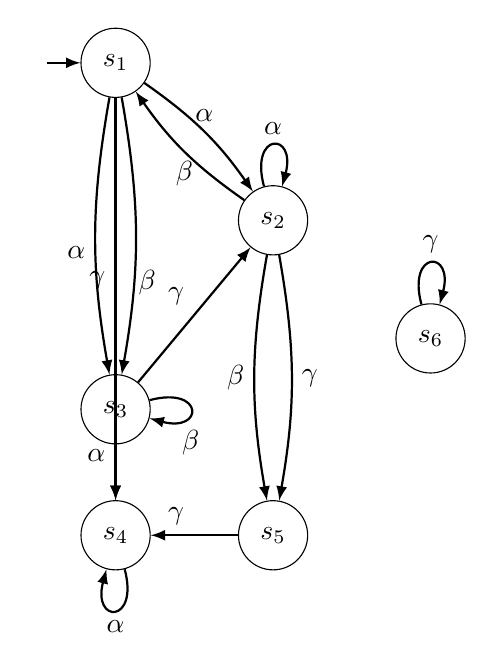
\begin{tikzpicture} [scale=2, every initial by arrow/.style={thick}]
		

		\path
		(\basex,		\basey) 		node[state,init] (s1) 	{$\state_1$} 
		(\basex+2,		\basey+0) 		node[state] (s2) 	{$\state_2$} 
		(\basex+1,		\basey-1.2) 	node[state] (s3) 	{$\state_3$} 
		(\basex,		\basey-2) 		node[state] (s4) 	{$\state_4$} 
		(\basex+2,		\basey-2) 		node[state] (s5) 	{$\state_5$}
		(\basex+3,		\basey-.75) 	node[state] (s6) 	{$\state_6$}
				
		;
		
%		
		\path [bendtrans] 	(s1) 	edge node [midway,above]				{\action} 		(s2);
		\path [bendtrans] 	(s1) 	edge node [near end,above right=-2pt]	{\actionb} 		(s3);
		\path [bendtransr] 	(s1) 	edge node [midway,below left]	{\action} 		(s3);
		\path [trans] 		(s1) 	edge node [midway,above left]	{\actionc} 		(s4);
		\path [bendtrans] 	(s2) 	edge node [midway,below]		{\actionb} 		(s1);
		\path [bendtransr] 	(s2) 	edge node [midway,left]			{\actionb} 		(s5);
		\path [bendtrans] 	(s2) 	edge node [midway,right]		{\actionc} 		(s5);
		\path [trans] 		(s3)	edge node [midway,above left]	{\actionc} 		(s2);
		\path [trans] 		(s3)	edge node [midway,above left]	{\action} 		(s4);
		\path [trans] 		(s5)	edge node [midway,above left]	{\actionc} 		(s4);
		
		\path [trans] 		(s2) 	edge [loop above] node [midway,above] {\action} 	(s2);
		\path [trans] 		(s3) 	edge [loop right] node [midway,below=4pt] {\actionb} 	(s3);
		\path [trans] 		(s4) 	edge [loop below] node [midway,below] {\action} 	(s4);
		\path [trans] 		(s6) 	edge [loop above] node [midway,above] {\actionc} 	(s6);
		
		
		%		midway, at start, near start, very near start, at end, near end, very near end
		
		
	\end{tikzpicture}
\end{document}
	\end{minipage}%
	\begin{minipage}{.5\textwidth}
		\hspace{5mm}
		\documentclass[tikz,preview]{standalone}
%\usepackage{prelude}

%%%%%%%%%%%%%%%%%%%%%%%%%%%%%%%%%%%% PACKAGES %%%%%%%%%%%%%%%%%%%%%%%%%%%%%%%%%%%%%%%%%%

\usepackage{inputenc,fontenc}
\usepackage[a4paper,margin=3cm]{geometry}
\usepackage[english]{babel}
%\usepackage[german]{babel}
%\usepackage[fixlanguage]{babelbib}


\usepackage{bbold}
\usepackage{amsthm}
\usepackage{amsmath}
\usepackage{amssymb} % doteqdot
\usepackage[dvipsnames]{xcolor}
\usepackage{standalone}
\usepackage{tikz}[mode=buildnew]
\usepackage{cite}
\usepackage{xspace}
\usepackage{relsize}
\usepackage{mathtools} % mathclap
%\usepackage{MnSymbol}
\usepackage{hyperref}
\usepackage{url}
\usepackage{listings} % for code
\usepackage[T1]{fontenc} %<
\hypersetup{
	colorlinks,
	citecolor=black,
	filecolor=black,
	linkcolor=black,
	urlcolor=black
}
\usepackage{pgfplots}
\pgfplotsset{compat=1.18}
%\usepackage{courier} %% Sets font for listing as Courier. But also for url and texttt!
\usepackage{listings, xcolor}
\usepackage{graphicx}
\usepackage{subcaption}

\usetikzlibrary{calc}
%\usepackage{xparse} % \newDocumentCommand for multiple optional arguments
%\usepackage{titlecaps}



%%%%%%%%%%%%%%%%%%%%%%%%%%%%%%%%%%%% THEOREMSTYLES %%%%%%%%%%%%%%%%%%%%%%%%%%%%%%%%%%

\theoremstyle{definition}
\newtheorem{definition}{Definition}[section]
\newtheorem{exmp}{Beispiel}[section]
%\AfterEndEnvironment{definition}{\noindent\ignorespaces}

\theoremstyle{theorem}
\newtheorem{theorem}{Satz}[section]
\newtheorem{proposition}{Proposition}[section]
%\AfterEndEnvironment{theorem}{\noindent\ignorespaces}

\theoremstyle{korollary}
\newtheorem{korollary}{Korollar}[section]
%\AfterEndEnvironment{korollary}{\noindent\ignorespaces}


\tikzset{
	mstate/.style={draw, circle, minimum size=.94cm}, 
	gstate/.style={draw, rectangle, minimum size=.8cm},
	varstate/.style={draw,rectangle, rounded corners, minimum size=1}, 
	trans/.style={draw, ->, thick},
	bendtrans/.style={draw, ->, thick, bend left=10},
	bendtransr/.style={draw, ->, thick, bend right=10},
	init/.style={initial, initial distance=6pt, initial text=},
	every loop/.style={min distance=5pt, looseness=8},
	>=latex
}
\usetikzlibrary{automata,positioning}

%auto shift/.style={auto=right,->,
%	to path={ let \p1=(\tikztostart),\p2=(\tikztotarget),
%		\n1={atan2(\y2-\y1,\x2-\x1)},\n2={\n1+180}
%		in ($(\tikztostart.{\n1})!1mm!270:(\tikztotarget.{\n2})$) -- 
%		($(\tikztotarget.{\n2})!1mm!90:(\tikztostart.{\n1})$) \tikztonodes}},

%%%%%%%%%%%%%%%%%%%%%%%%%%%%%%%%%%% MY MACROS %%%%%%%%%%%%%%%%%%%%%%%%%%%%%%%%%%%%%%%%%
%formatting
\newcommand{\comment}[2]{{\color{#1}#2}}
\newcommand{\redcomment}[1]{{\color{red}#1}}
\newcommand{\purpcomment}[1]{{\color{pink}#1}}
\newcommand{\bluecomment}[1]{{\color{blue}#1}}
\newcommand{\mt}[1]{\ensuremath{{#1}}\xspace}
\newcommand{\mynewcommand}[2]{\newcommand{#1}{\mt{#2}}} %% currently not used becaue of ide highlighting
\newcommand{\arr}{\mt{\to}}

%model checking terms
\newcommand{\mimicrel}{\mt{\mathcal{R}}}
\newcommand{\bisimeq}{\mt{\;\!\sim\;\!}}
\newcommand{\simorder}{\mt{\;\!\preceq\;\!}}
\newcommand{\simequiv}{\mt{\;\!\simeq\;\!}} %command already defined
\newcommand{\relts}{\mt{\;\!\bullet_{_{\tiny{TS}}}\;\!}}
\newcommand{\rel}{\mt{\;\!\bullet\;\!}}

%own names
\newcommand{\nm}[1]{#1\xspace}
\newcommand{\mdpN}{\nm{MDP}}
\newcommand{\mdpsN}{\nm{MDPs}}
\newcommand{\viewN}{\nm{view}}
\newcommand{\viewNC}{\nm{View}}
\newcommand{\viewsN}{\nm{views}}
\newcommand{\viewsNC}{\nm{Views}}
\newcommand{\grpfctsubN}{\nm{detached grouping function}}
\newcommand{\grpfctsubNC}{\nm{detached grouping function}}
\newcommand{\grpfctsubNCC}{\nm{Detached Grouping Function}}
\newcommand{\grpfctN}{\nm{grouping function}}
\newcommand{\grpfctNC}{\nm{Grouping function}}
\newcommand{\grpfctNCC}{\nm{Grouping Function}}
\newcommand{\grpfctsN}{\nm{grouping functions}}
\newcommand{\grpfctsNC}{\nm{Grouping functions}}
\newcommand{\grpfctsNCC}{\nm{Grouping Functions}}
\newcommand{\stmimicN}{\nm{state-mimic}}
\newcommand{\stmimicsN}{\nm{state-mimics}}
\newcommand{\stmimickingN}{\nm{state-mimicking}}
\newcommand{\stmimickedN}{\nm{state-mimicked}}
%\newcommand{\chosenphtypeNCC}{\nm{Transition System}}
%\newcommand{\chgphNC}{\nm{Transition system}}
%\newcommand{\chgphN}{\nm{transition system}}
%\newcommand{\chgphsNCC}{\nm{Transition Systems}}
%\newcommand{\chgphsNC}{\nm{Transition systems}}
%\newcommand{\chgphsN}{\nm{transition systems}}
\newcommand{\chgphNCC}{\nm{MDP}}
\newcommand{\chgphNC}{\nm{MDP}}
\newcommand{\chgphN}{\nm{MDP}}
\newcommand{\achgphN}{\nm{an MDP}}
\newcommand{\chgphsNCC}{\nm{MDPs}}
\newcommand{\chgphsNC}{\nm{MDPs}}
\newcommand{\chgphsN}{\nm{MDPs}}
\newcommand{\parllcompN}{\nm{parallel composition}}
\newcommand{\parllcompNC}{\nm{Parallel composition}}
\newcommand{\parllcompNCC}{\nm{Parallel Composition}}
\newcommand{\parllcompsN}{\nm{parallel compositions}}
\newcommand{\parllcompsNC}{\nm{Parallel compositions}}
\newcommand{\parllcompsNCC}{\nm{Parallel Compositions}}
\newcommand{\sccN}{\nm{SCC}}
\newcommand{\sccsN}{\nm{SCCs}}
\newcommand{\bsccN}{\nm{BSCC}}
\newcommand{\bsccsN}{\nm{BSCCs}}
\newcommand{\jgrapht}{\nm{jGraphtT}}

\newcommand{\outactident}{\nm{OutActionsIdent}}

%names
\newcommand{\iffN}{\nm{if and only if}}
\newcommand{\tsN}{\nm{TS}}

%% outactions identical
\newcommand{\outactidentstrong}{\nm{strong}}
\newcommand{\outactidentweak}{\nm{weak}}

% CORE DEFINITIONS
\newcommand{\grpfct}[1][\viewppty]{\mt{F_{#1}}}
\newcommand{\grpfctsub}[1][\viewppty]{\mt{\tilde{F}_{#1}}}
%\newcommand{\grpfctimg}[1]{\mt{{\grpfct}[{#1}]}}
%\newcommand{\fctimg}[2]{\mt{{#1}[{#2}]}}
\newcommand{\eqrelview}{\mt{R}}
\newcommand{\eqclassv}[1][\state]{\mt{\eqclass{#1}{\eqrelview}}}
\newcommand{\eqclasssetv}[1][\states]{\mt{{#1}/\eqrelview}} %OLD: \bigcup_{\state \in \states} \eqclassv
\newcommand{\viewid}{\mt{\mdp}}
\newcommand{\view}[1][\viewppty]{\mt{\viewid_{#1}}}
\newcommand{\imggrp}{\mt{\arbset}}
\newcommand{\imggrpsub}{\mt{X}}
\newcommand{\viewppty}{\mt{\theta}}
\newcommand{\pll}{\mt{\;\!\pllpure\;\!}}
\newcommand{\pllrev}{\mt{\pllpure^{-1}}}
\newcommand{\pllpure}{\mt{||}}
\newcommand{\compselectset}{\mt{Z}}
\newcommand{\compselectpure}{\mt{\pllpure_\compselectset}}
\newcommand{\compselect}{\mt{\;\pllpure_\compselectset\;}}
\newcommand{\remstates}{\mt{\bigcup_{\state \in \states \setminus \states_1}\{\{\state\}\}}}
\newcommand{\nogroupstates}[1][\states_2]{\mt{\bigcup_{\state \in \states \setminus {#1}}\{\{\state\}\}}}
\newcommand{\remelem}{\mt{\bullet}}
\newcommand{\nogroupset}{\mt{\xi}}
\newcommand{\remset}{\mt{\{\remelem\}}}
\newcommand{\gfctpll}{\mt{\grpfct[\pll]}}
\newcommand{\group}{\mt{\top}}
\newcommand{\imggrpbinview}{\mt{\{\remelem, \notppty\}}}
\newcommand{\viewappset}{\mt{\tilde{\states}}}
\newcommand{\hasppty}{\mt{\top}}
\newcommand{\notppty}{\mt{\bot}}
\newcommand{\disregardelem}{\mt{\Delta}}
\newcommand{\disregardelements}{\mt{{\disregardelem_1, \dots, \disregardelem_n}}}



%\newcommand{\mdp}{def}\mdp
%\newcommand{\mdpdef}



% EXAMPLE VIEWS
\newcommand{\pptyatomicprops}{\mt{\atomicprops}}
\newcommand{\pptyinitstates}{\mt{\initstates}}
\newcommand{\pptyinactsetsize}{\mt{|\inacts(\state)|}}
\newcommand{\pptyhasoutact}{\mt{\exists\outact}}
\newcommand{\pptyminoutact}[2]{\mt{#1\leq#2}}
\newcommand{\pptymaxoutact}[2]{\mt{#2\leq#1}}
\newcommand{\pptyspanoutact}[3]{\mt{#1\leq#2\leq#3}}
\newcommand{\pptyoutactsetsize}{\mt{|\outacts(\state)|}}
\newcommand{\pptyoutactsingle}{\mt{|\outacts(\state)|_1}}
\newcommand{\pptystrongoutactident}{\mt{\outacts(\state)_=}}
\newcommand{\pptyweakoutactident}{\mt{\outacts(\state)_\approx}}
\newcommand{\pptyhasinact}{\mt{\exists\inact}}
\newcommand{\pptymininact}[2]{\mt{#1\leq#2}}
\newcommand{\pptymaxinact}[2]{\mt{#2\leq#1}}
\newcommand{\pptyspaninact}[3]{\mt{#1\leq#2\leq#3}}
\newcommand{\pptyinactsingle}{\mt{|\inacts(\state)|_1}}
\newcommand{\pptystronginactident}{\mt{\inacts(\state)_=}}
\newcommand{\pptyweakinactident}{\mt{\inacts(\state)_\approx}}
\newcommand{\pptyparamvalueseq}{\mt{\var = \varval}}
\newcommand{\pptyparamvaluesneq}{\mt{\var \neq \varval}}
\newcommand{\pptyparamdnf}{\mt{VarDNF}}
\newcommand{\pptyparamcnf}{\mt{VarCNF}}
\newcommand{\pptyparamvalueseqopt}{\mt{\var = \varval}}
\newcommand{\pptyparamvalident}{\mt{Var:\varval}}
\newcommand{\pptydistance}{\mt{\distpath}}
\newcommand{\pptydistancerev}{\mt{\distpathrev}}
\newcommand{\pptydistancebi}{\mt{\distpathbi}}
\newcommand{\pptyhascycle}{\mt{\exists\cycle}}
\newcommand{\pptyexactactcycle}{\mt{\{\cycle_{\action,n}\}}}
\newcommand{\pptycycleset}{\mt{\cup{\{\state\}_\cycle}}}
\newcommand{\pptyexactcycle}{\mt{\{\cycle_n\}}}
\newcommand{\pptyscc}{\mt{scc}}
\newcommand{\pptybscc}{\mt{bscc}}
\newcommand{\pptyprop}{\mt{\redcomment{?}}}
\newcommand{\pptyident}{id}


\newcommand{\gfctatomicprops}{\mt{\grpfct[\pptyatomicprops]}}
\newcommand{\gfctinitstates}{\mt{\grpfct[\pptyinitstates]^\hasppty}}
\newcommand{\gfcthasoutaction}{\mt{\grpfct[\pptyhasoutact]^\hasppty}}
\newcommand{\gfctminoutaction}{\mt{\grpfct[\pptyminoutact{\numoutact}{\outact}]^\hasppty}}
\newcommand{\gfctmaxoutaction}{\mt{\grpfct[\pptymaxoutact{\numoutact}{\outact}]^\hasppty}}
\newcommand{\gfctspanoutaction}{\mt{\grpfct[\pptyspanoutact{\numoutactb}{\outact}{\numoutact}]^\hasppty}}
\newcommand{\gfctoutactsetsize}{\mt{\grpfct[\pptyoutactsetsize]}}
\newcommand{\gfctoutactsingle}{\mt{\grpfct[\pptyoutactsingle]^\notppty}}
\newcommand{\gfctstrongoutactident}{\mt{\grpfct[\pptystrongoutactident]}}
\newcommand{\gfctweakoutactident}{\mt{\grpfct[\pptyweakoutactident]}}
\newcommand{\gfcthasinaction}{\mt{\grpfct[\pptyhasinact]^\hasppty}}
\newcommand{\gfctmininaction}{\mt{\grpfct[\pptymininact{\numinact}{\inact}]^\hasppty}}
\newcommand{\gfctmaxinaction}{\mt{\grpfct[\pptymaxinact{\numinact}{\inact}]^\hasppty}}
\newcommand{\gfctspaninaction}{\mt{\grpfct[\pptyspaninact{\numinactb}{\inact}{\numinact}]^\hasppty}}
\newcommand{\gfctinactsetsize}{\mt{\grpfct[\pptyinactsetsize]}}
\newcommand{\gfctinactsingle}{\mt{\grpfct[\pptyinactsingle]^\notppty}}
\newcommand{\gfctstronginactident}{\mt{\grpfct[\pptystronginactident]}}
\newcommand{\gfctweakinactident}{\mt{\grpfct[\pptyweakinactident]}}
\newcommand{\gfctparamvalueseq}{\mt{\grpfct[\pptyparamvalueseq]^\hasppty}}
\newcommand{\gfctparamvaluesneq}{\mt{\grpfct[\pptyparamvaluesneq]^\hasppty}}
\newcommand{\gfctparamdnf}{\mt{\grpfct[\pptyparamdnf]^\hasppty}}
\newcommand{\gfctparamcnf}{\mt{\grpfct[\pptyparamcnf]^\hasppty}}
\newcommand{\gfctparamvalueseqopt}{\mt{\pptyparamvalueseqopt}}
\newcommand{\gfctparamvalident}{\mt{\grpfct[\pptyparamvalident]}}
\newcommand{\gfctdistance}{\mt{\grpfct[\pptydistance]}}
\newcommand{\gfctdistancerev}{\mt{\grpfct[\pptydistancerev]}}
\newcommand{\gfctdistancebi}{\mt{\grpfct[\pptydistancebi]}}
\newcommand{\gfcthascycle}{\mt{\grpfct[\pptyhascycle]}}
\newcommand{\gfctexactcycle}{\mt{\grpfct[\pptyexactcycle]}}
\newcommand{\gfctcycleset}{\mt{\grpfct[\pptycycleset]}}
\newcommand{\gfctexactactcycle}{\mt{\grpfct[\pptyexactactcycle]}}
\newcommand{\gfctscc}{\mt{\grpfct[\pptyscc]}}
\newcommand{\gfctbscc}{\mt{\grpfct[\pptybscc]}}
\newcommand{\gfctprop}{\mt{\grpfct[\pptyprop]}}
\newcommand{\gfctident}{\mt{\grpfct[\pptyident]}}

\newcommand{\gfctsubatomicprops}{\mt{\grpfctsub[\pptyatomicprops]}}
\newcommand{\gfctsubinitstates}{\mt{\grpfctsub[\pptyinitstates]^\hasppty}}
\newcommand{\gfctsubhasoutaction}{\mt{\grpfctsub[\pptyhasoutact]^\hasppty}}
\newcommand{\gfctsubminoutaction}{\mt{\grpfctsub[\pptyminoutact{\numoutact}{\outact}]^\hasppty}}
\newcommand{\gfctsubmaxoutaction}{\mt{\grpfctsub[\pptymaxoutact{\numoutact}{\outact}]^\hasppty}}
\newcommand{\gfctsubspanoutaction}{\mt{\grpfctsub[\pptyspanoutact{\numoutactb}{\outact}{\numoutact}]^\hasppty}}
\newcommand{\gfctsuboutactsetsize}{\mt{\grpfctsub[\pptyoutactsetsize]}}
\newcommand{\gfctsuboutactsingle}{\mt{\grpfctsub[\pptyoutactsingle]^\notppty}}
\newcommand{\gfctsubstrongoutactident}{\mt{\grpfctsub[\pptystrongoutactident]^\hasppty}}
\newcommand{\gfctsubweakoutactident}{\mt{\grpfctsub[\pptyweakoutactident]^\hasppty}}
\newcommand{\gfctsubhasinaction}{\mt{\grpfctsub[\pptyhasinact]}}
\newcommand{\gfctsubmininaction}{\mt{\grpfctsub[\pptymininact{\numinact}{\inact}]}}
\newcommand{\gfctsubmaxinaction}{\mt{\grpfctsub[\pptymaxinact{\numinact}{\inact}]}}
\newcommand{\gfctsubspaninaction}{\mt{\grpfctsub[\pptyspaninact{\numinactb}{\inact}{\numinact}]}}
\newcommand{\gfctsubinactsetsize}{\mt{\grpfctsub[\pptyinactsetsize]^\hasppty}}
\newcommand{\gfctsubinactsingle}{\mt{\grpfctsub[\pptyinactsingle]^\notppty}}
\newcommand{\gfctsubstronginactident}{\mt{\grpfctsub[\pptystronginactident]}}
\newcommand{\gfctsubweakinactident}{\mt{\grpfctsub[\pptyweakinactident]}}
\newcommand{\gfctsubparamvalueseq}{\mt{\grpfctsub[\pptyparamvalueseq]^\hasppty}}
\newcommand{\gfctsubparamvaluesneq}{\mt{\grpfctsub[\pptyparamvaluesneq]^\hasppty}}
\newcommand{\gfctsubparamdnf}{\mt{\grpfctsub[\pptyparamdnf]^\hasppty}}
\newcommand{\gfctsubparamcnf}{\mt{\grpfctsub[\pptyparamcnf]^\hasppty}}
\newcommand{\gfctsubparamvalueseqopt}{\mt{\pptyparamvalueseqopt}}
\newcommand{\gfctsubparamvalident}{\mt{\grpfctsub[\pptyparamvalident]}}
\newcommand{\gfctsubdistance}{\mt{\grpfctsub[\pptydistance]}}
\newcommand{\gfctsubdistancerev}{\mt{\grpfctsub[\pptydistancerev]}}
\newcommand{\gfctsubdistancebi}{\mt{\grpfctsub[\pptydistancebi]}}
\newcommand{\gfctsubhascycle}{\mt{\grpfctsub[\pptyhascycle]^\hasppty}}
\newcommand{\gfctsubexactcycle}{\mt{\grpfctsub[\pptyexactcycle]}}
\newcommand{\gfctsubcycleset}{\mt{\grpfctsub[\pptycycleset]}}
\newcommand{\gfctsubexactactcycle}{\mt{\grpfctsub[\pptyexactactcycle]}}
\newcommand{\gfctsubscc}{\mt{\grpfctsub[\pptyscc]}}
\newcommand{\gfctsubbscc}{\mt{\grpfctsub[\pptybscc]}}
\newcommand{\gfctsubprop}{\mt{\grpfctsub[\pptyprop]}}
\newcommand{\gfctsubident}{\mt{\grpfctsub[\pptyident]}}


\newcommand{\viewatomicprops}{\mt{\view[\pptyatomicprops]}}
\newcommand{\viewinitstates}{\mt{\view[\pptyinitstates]^\hasppty}}
\newcommand{\viewhasoutaction}{\mt{\view[\pptyhasoutact]^\hasppty}}
\newcommand{\viewminoutaction}{\mt{\view[\pptyminoutact{\numoutact}{\outact}]^\hasppty}}
\newcommand{\viewmaxoutaction}{\mt{\view[\pptymaxoutact{\numoutact}{\outact}]^\hasppty}}
\newcommand{\viewspanoutaction}{\mt{\view[\pptyspanoutact{\numoutactb}{\outact}{\numoutact}]^\hasppty}}
\newcommand{\viewoutactsetsize}{\mt{\view[\pptyoutactsetsize]}}
\newcommand{\viewoutactsingle}{\mt{\view[\pptyoutactsingle]^\notppty}}
\newcommand{\viewstrongoutactident}{\mt{\view[\pptystrongoutactident]}}
\newcommand{\viewweakoutactident}{\mt{\view[\pptyweakoutactident]}}
\newcommand{\viewhasinaction}{\mt{\view[\pptyhasinact]^\hasppty}}
\newcommand{\viewmininaction}{\mt{\view[\pptymininact{\numinact}{\inact}]^\hasppty}}
\newcommand{\viewmaxinaction}{\mt{\view[\pptymaxinact{\numinact}{\inact}]^\hasppty}}
\newcommand{\viewspaninaction}{\mt{\view[\pptyspaninact{\numinactb}{\inact}{\numinact}]^\hasppty}}
\newcommand{\viewinactsetsize}{\mt{\view[\pptyinactsetsize]}}
\newcommand{\viewinactsingle}{\mt{\view[\pptyinactsingle]^\notppty}}
\newcommand{\viewstronginactident}{\mt{\view[\pptystronginactident]}}
\newcommand{\viewweakinactident}{\mt{\view[\pptyweakinactident]}}
\newcommand{\viewparamvalueseq}{\mt{\view[\pptyparamvalueseq]}}
\newcommand{\viewparamvaluesneq}{\mt{\view[\pptyparamvaluesneq]}}
\newcommand{\viewparamdnf}{\mt{\view[\pptyparamdnf]^\hasppty}}
\newcommand{\viewparamcnf}{\mt{\view[\pptyparamcnf]^\hasppty}}
\newcommand{\viewparamvalueseqopt}{\mt{\pptyparamvalueseqopt}}
\newcommand{\viewparamvalident}{\mt{\view[\pptyparamvalident]}}
\newcommand{\viewdistance}{\mt{\view[\pptydistance]}}
\newcommand{\viewdistancerev}{\mt{\view[\pptydistancerev]}}
\newcommand{\viewdistancebi}{\mt{\view[\pptydistancebi]}}
\newcommand{\viewhascycle}{\mt{\view[\pptyhascycle]}}
\newcommand{\viewexactcycle}{\mt{\view[\pptyexactcycle]}}
\newcommand{\viewcycleset}{\mt{\view[\pptycycleset]}}
\newcommand{\viewexactactcycle}{\mt{\view[\pptyexactactcycle]}}
\newcommand{\viewscc}{\mt{\view[\pptyscc]}}
\newcommand{\viewbscc}{\mt{\view[\pptybscc]}}
\newcommand{\viewprop}{\mt{\view[\pptyprop]}}
\newcommand{\viewident}{\mt{\view[\pptyident]}}

%\newcommand{\viewatomicprops}{\mt{\view[\atomicprops]}}
%\newcommand{\viewinitstates}{\mt{\view[\initstates]}}
%\newcommand{\viewhasoutaction}{\mt{\view[\pptyhasoutact]}}
%\newcommand{\viewminoutaction}{\mt{\view[\pptyminoutact{\numoutact}{\outact}]}}
%\newcommand{\viewmaxoutaction}{\mt{\view[\pptymaxoutact{\numoutact}{\outact}]}}
%\newcommand{\viewspanoutaction}{\mt{\view[\pptyspanoutact{\numoutactb}{\outact}{\numoutact}]}}
%\newcommand{\viewoutactsetsize}{\mt{\view[\pptyoutactsetsize]}}
%\newcommand{\viewoutactsingle}{\mt{\view[\pptyoutactsingle]}}
%\newcommand{\viewstrongoutactident}{\mt{\view[\outacts(\state)_=]}}
%\newcommand{\viewweakoutactident}{\mt{\view[\outacts(\state)_\approx]}}
%\newcommand{\viewhasinaction}{\mt{\view[\pptyhasinact]}}
%\newcommand{\viewmininaction}{\mt{\view[\pptymininact{\numinact}{\inact}]}}
%\newcommand{\viewmaxinaction}{\mt{\view[\pptymaxinact{\numinact}{\inact}]}}
%\newcommand{\viewspaninaction}{\mt{\view[\pptyspaninact{\numinactb}{\inact}{\numinact}]}}
%\newcommand{\viewinactsetsize}{\mt{\view[\pptyinactsetsize]}}
%\newcommand{\viewinactsingle}{\mt{\view[\pptyinactsingle]}}
%\newcommand{\viewstronginactident}{\mt{\view[\inacts(\state)_=]}}
%\newcommand{\viewweakinactident}{\mt{\view[\inacts(\state)_\approx]}}
%\newcommand{\viewparamvalueseq}{\mt{\view[\var = \varval]}}
%\newcommand{\viewparamvaluesneq}{\mt{\view[\var \neq \varval]}}
%\newcommand{\viewparamdnf}{\mt{\view[VarDNF]}}
%\newcommand{\viewparamcnf}{\mt{\view[VarCNF]}}
%\newcommand{\viewparamvalident}{\mt{\view[\pptyparamvalident]}}
%\newcommand{\viewdistance}{\mt{\view[\pptydistance]}}
%\newcommand{\viewhascycle}{\mt{\view[\exists\cycle]}}
%\newcommand{\viewexactcycle}{\mt{\view[\pptyexactcycle]}}
%\newcommand{\viewcycleset}{\mt{\view[\pptycycleset]}}
%\newcommand{\viewexactactcycle}{\mt{\view[\pptyexactactcycle]}}
%\newcommand{\viewscc}{\mt{\view[scc]}}
%\newcommand{\viewbscc}{\mt{\view[bscc]}}

%actions
\newcommand{\numoutact}{\mt{n}}
\newcommand{\numoutactb}{\mt{m}}
\newcommand{\numinact}{\mt{n}}
\newcommand{\numinactb}{\mt{m}}

\newcommand{\predmaxoutact}[1][\numoutact]{\mt{Q_{\outact\leq#1}(\state,\state_1, \dots, \state_{#1+1})}}
\newcommand{\predminoutact}[1][\numoutact]{\mt{Q_{#1\leq\outact}(\state,\state_1, \dots, \state_{#1})}}
\newcommand{\formoutact}[1][\state]{\mt{C_{#1,\outact}}}
\newcommand{\predmaxinact}[1][\numinact]{\mt{Q_{\inact\leq#1}(\state,\state_1, \dots, \state_{#1+1})}}
\newcommand{\predmininact}[1][\numinact]{\mt{Q_{#1\leq\inact}(\state,\state_1, \dots, \state_{#1})}}

\newcommand{\outact}[1][\action]{\mt{\overrightarrow{#1}}}
\newcommand{\outacts}{\mt{\overrightarrow{\actions}}}
\newcommand{\inact}{\mt{\overleftarrow{\action}}}
\newcommand{\inacts}[1][\action]{\mt{\overleftarrow{#1}}}

%%Parameters
\newcommand{\vars}[1][\mdp]{\mt{V\!ar_{#1}}}
\newcommand{\var}{\mt{x}}
\newcommand{\varstate}[1][]{\mt{\var_{\state#1}}}
\newcommand{\varval}{\mt{a}}
\newcommand{\vareval}[1][\mdp]{\mt{V\!arEval_{#1}}}
\newcommand{\varevalimg}[1][\mdp]{\mt{\vareval[#1][\states,\vars]}}
\newcommand{\varevalimgset}{\mt{\arbset}}
\newcommand{\someparam}{\mt{\tilde{x}}}
\newcommand{\eqorneq}{\mt{\;\doteqdot\;}}
\newcommand{\varstyle}[2]{\mt{\langle#1,#2\rangle}}




%\makeatletter
%\newcommand{\overleftrightsmallarrow}{\mathpalette{\overarrowsmall@\leftrightarrowfill@}}
%\newcommand{\overrightsmallarrow}{\mathpalette{\overarrowsmall@\rightarrowfill@}}
%\newcommand{\overleftsmallarrow}{\mathpalette{\overarrowsmall@\leftarrowfill@}}
%\newcommand{\overarrowsmall@}[3]{%
%	\vbox{%
%		\ialign{%
%			##\crcr
%			#1{\smaller@style{#2}}\crcr
%			\noalign{\nointerlineskip}%
%			$\m@th\hfil#2#3\hfil$\crcr
%		}%
%	}%
%}
%\def\smaller@style#1{%
%	\ifx#1\displaystyle\scriptstyle\else
%	\ifx#1\textstyle\scriptstyle\else
%	\scriptscriptstyle
%	\fi
%	\fi
%}
%\makeatother
%\newcommand{\te}[1]{\overleftrightsmallarrow{#1}}

% Distance
\newcommand{\fctdist}{\mt{distance}}
\newcommand{\fctdistdefault}{\mt{\fctdist(\chgph, \smstates, \grandist)}}
\newcommand{\distval}{\mt{d}}
\newcommand{\grandist}{\mt{n}}
\let\path\oldpath
\newcommand{\path}{\mt{P}}
\newcommand{\pathbi}{\mt{\bar{\path}}}
\newcommand{\pathsecfull}{\mt{(\state_0, \action_0, \state_1, \action_1, \dots, \action_{n}, \state_{n+1})}}
\newcommand{\lenpath}{\mt{len}}
\newcommand{\pfirst}{\mt{first}}
\newcommand{\plast}{\mt{last}}
\newcommand{\pathset}{\mt{\path_\chgph}}
\newcommand{\pathbiset}{\mt{\pathbi_\chgph}}
\newcommand{\distpath}{\mt{\overrightarrow{dist}}}
\newcommand{\distpathrev}{\mt{\overleftarrow{dist}}}
\newcommand{\distpathbi}{\mt{\overline{dist}}}
%Cycles
\newcommand{\cyclesecfull}{\mt{(\state_0, \action_0, \state_1, \action_1, \dots, \action_{n-1}, \state_0)}}
\newcommand{\fctfindcycles}{\mt{findCycles}}
\newcommand{\cycle}{\mt{C}}
\newcommand{\cycleset}{\mt{\cycle_{\mdp, n}}}
\newcommand{\lencycle}{\mt{len}}
% strongly connected components
\newcommand{\scc}{\mt{T}}
\newcommand{\setscc}{\mt{SCC_{\chgph,n}}}
\newcommand{\setbscc}{\mt{BSCC_{\chgph,n}}}

% properties
\newcommand{\propfct}{\mt{f}}

% all Systems
\newcommand{\chgph}{\mt{\mdp}}
\newcommand{\chgphtuple}{\mt{\mdptuple}}
\newcommand{\chgphtupledist}{\mt{\mdptupledist}}

\newcommand{\states}{\mt{S}}
\newcommand{\actions}{\mt{Act}}
\newcommand{\atomicprops}{\mt{AP}}
\newcommand{\labelingfct}{\mt{L}}
\newcommand{\init}{\mt{\initdistrib}} % use MDP % refers to the underlying set
\newcommand{\trans}{\mt{\probtfunc}} % use MDP % refers to the underlying set
\newcommand{\smstates}{\mt{\tilde{\states}}}


\newcommand{\state}{\mt{s}}
\newcommand{\action}{\mt{\alpha}}
\newcommand{\actionb}{\mt{\beta}}
\newcommand{\actionc}{\mt{\gamma}}
\newcommand{\smstate}{\mt{\tilde{\state}}}



% transition sysstems
\newcommand{\ts}{\mt{TS}}
\newcommand{\transitionrel}{\mt{\longrightarrow}}
\newcommand{\initstates}{\mt{I}}
\newcommand{\transitionsystem}{\mt
	{(\states, \actions, \transitionrel, \initstates, \atomicprops, \labelingfct)}
}
\newcommand{\tstupledist}{\mt{(\states', \actions',\transitionrel', \initstates', \labelingfct')}}


%Markov chains and MDP
\newcommand{\mdp}{\mt{\autm}}
\newcommand{\mdptuple}{\mt{(\states, \actions, \probtfunc, \initdistrib, \atomicprops, \labelingfct)}}
\newcommand{\mdptupledist}{\mt{(\states', \actions', \probtfunc', \initdistrib', \atomicprops', \labelingfct')}}
\newcommand{\autm}{\mt{\mathcal{M}}}
\newcommand{\probtfunc}{\mt{\textbf{P}}}
\newcommand{\initdistrib}{\mt{\iota_{init}}}


%maths
\newcommand{\powerset}[1]{\mt{\mathcal{P}(#1)}}
\newcommand{\eqclass}[2]{\mt{[#1]_{#2}}}%{\mt{#1 / #2}}
\newcommand{\impr}{\mt{\hspace{3mm}\Rightarrow\hspace{2mm}}}
\newcommand{\impl}{\mt{\hspace{3mm}\Leftarrow\hspace{2mm}}}
\newcommand{\natnums}{\mt{\mathbb{N}}} 
\newcommand{\realnums}{\mt{\mathbb{R}}}
\newcommand{\intmodn}[1][n]{\mt{\mathbb{Z}_{#1}}}
\newcommand{\arbset}{\mt{M}}
\newcommand{\bigsum}[2][]{\mt{\mathlarger{\sum}_{#2}^{#1}}}
\newcommand{\bbigsum}[2][]{\mt{\mathlarger{\mathlarger{\sum}}_{#2}^{#1}}}
\newcommand{\invimage}[2]{#1^{\mt{-1}(#2)}}
\newcommand{\img}{\mt{Img}}
\newcommand{\cond}{\mt{\,|\,}}

%tickz
%% \definecolor{darkred}{RGB}{196, 42, 42}

%implementation
\newcommand{\pmcvis}{\nm{PMC-Vis}}





\begin{document}
	\newcommand{\basex}{0}
	\newcommand{\basey}{0}
	\newcommand{\createstate}[3]{\node[draw, circle, minimum size=1cm] (#1) at (#2) {#3}}
	
	
	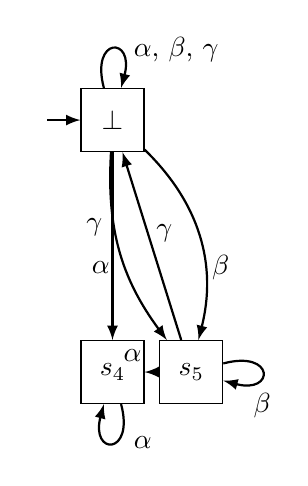
\begin{tikzpicture} [scale=2, every initial by arrow/.style={thick}]
		
		
		\path
		(\basex,		\basey-.4) 		node[gstate,init] (sbot) 	{$\notppty$} 		
		(\basex,		\basey-2) 		node[gstate] (s4) 	{$\state_4$} 
		(\basex+1.5,	\basey-2) 		node[gstate] (s5) 	{$\state_5$} 
		
		;
		
		%		
		\path [trans, bend left=30] 	(sbot) 	edge node [near end,above right=-2pt]	{\actionb} 		(s5);
		\path [trans, bend right=20] 	(sbot) 	edge node [midway,below left]	{\action} 		(s5);
		\path [trans] 		(sbot) 	edge node [midway,above left]	{\actionc} 		(s4);
		\path [trans] 		(s5)	edge node [midway,above right=-3pt]	{\actionc} 		(sbot);
		\path [trans] 		(s5)	edge node [midway,above left]	{\action} 		(s4);
		
		\path [trans] 	(sbot) 	edge [loop above] node [right=4pt]	{\action, \actionb, \actionc} 		(sbot);
%		\path [bendtrans] 	(sbot) 	edge node [midway,below]		{\actionb} 		(sbot);
%		\path [bendtransr] 	(sbot) 	edge node [midway,left]			{\actionb} 		(sbot);
%		\path [bendtrans] 	(sbot) 	edge node [midway,right]		{\actionc} 		(sbot);
		
%		\path [trans] 		(sbot) 	edge [loop above] node [midway,above] {\action} 	(sbot);
		\path [trans] 		(s5) 	edge [loop right] node [midway,below=4pt] {\actionb} 	(s5);
		\path [trans] 		(s4) 	edge [loop below] node [midway,right=4pt] {\action} 	(s4);
%		\path [trans] 		(sbot) 	edge [loop above] node [midway,above] {\actionc} 	(sbot);
		
		
		%		midway, at start, near start, very near start, at end, near end, very near end
		
		
	\end{tikzpicture}
\end{document}
	\end{minipage}
	\caption{Simplified representations of \mdp (left) and the \viewN $\view[\pptyspanoutact{1}{\outact}{1}]$ on it (right)}
	\label{fig:outActSpan}
\end{figure}


The \viewsN above can be combined with \parllcompN. The thereby obtained \viewN requires that the respective conditions of all the combined \viewsN are met. In this sense it is a conjunctive combination.

Instead of making requirements about states and group them based on whether they meet these requirements it also possible to group states that are very similar or even identical in regard to their outaction. We consider this idea with the \emph{\outactident \viewNC} in two variants: \outactidentstrong and \outactidentweak (idententiy). Firstly we will consider the variant of strong identity.

\begin{definition}
	Let $\chgph = \chgphtuple$ be \achgphN and $\action \in \actions$. The \viewN \viewstrongoutactident is defined by its \grpfctN $\gfctstrongoutactident : \states \to \imggrp$ with
	\[
	\state \mapsto	
	\{(\action, \numoutact) \mid \action \in \actions, \numoutact \text{ is the number of times that \action is outgoing from } \state\}
	\]
	and $\imggrp := \actions \times \natnums_0 \cup \remset$.
\end{definition}

The \grpfctN asserts to each state a set of pairs. Note that a pair is contained int the set for each action $\action \in \actions$. In case there is no outgoing transition from state \state with an action \action it is $(\action, 0) \in \gfctstrongoutactident$. For $\state_1, \state_2 \in \states$ it is $\gfctstrongoutactident(\state_1) = \gfctstrongoutactident(\state_2)$ \iffN $\state_1$ and $\state_2$ are mapped to the same set of pairs. By Definition \ref{def:eqrelview} the obtained equivalence classes of \eqrelview are
\[
	\eqclassv := \{\state \in \states \mid \gfctstrongoutactident(\state) = \{(\action_1, \numoutact_1), \dots, (\action_l, \numoutact_l)\}, l = |\actions|\}
\]
According to Definition \ref{def:view} the set $\states' := \bigcup_{\state \in \states} \eqclassv$ is the set of states of \viewstrongoutactident. All other components of \viewstrongoutactident are as usual structured in accordance with the Definition \ref{def:view}.
As mentioned earlier a \outactidentweak variant of the \outactident \viewN is also conceivable.

\begin{figure}[h]
	\begin{minipage}{.5\textwidth}
		\hspace{5mm}
		\documentclass[tikz,preview]{standalone}
%\usepackage{prelude}

%%%%%%%%%%%%%%%%%%%%%%%%%%%%%%%%%%%% PACKAGES %%%%%%%%%%%%%%%%%%%%%%%%%%%%%%%%%%%%%%%%%%

\usepackage{inputenc,fontenc}
\usepackage[a4paper,margin=3cm]{geometry}
\usepackage[english]{babel}
%\usepackage[german]{babel}
%\usepackage[fixlanguage]{babelbib}


\usepackage{bbold}
\usepackage{amsthm}
\usepackage{amsmath}
\usepackage{amssymb} % doteqdot
\usepackage[dvipsnames]{xcolor}
\usepackage{standalone}
\usepackage{tikz}[mode=buildnew]
\usepackage{cite}
\usepackage{xspace}
\usepackage{relsize}
\usepackage{mathtools} % mathclap
%\usepackage{MnSymbol}
\usepackage{hyperref}
\usepackage{url}
\usepackage{listings} % for code
\usepackage[T1]{fontenc} %<
\hypersetup{
	colorlinks,
	citecolor=black,
	filecolor=black,
	linkcolor=black,
	urlcolor=black
}
\usepackage{pgfplots}
\pgfplotsset{compat=1.18}
%\usepackage{courier} %% Sets font for listing as Courier. But also for url and texttt!
\usepackage{listings, xcolor}
\usepackage{graphicx}
\usepackage{subcaption}

\usetikzlibrary{calc}
%\usepackage{xparse} % \newDocumentCommand for multiple optional arguments
%\usepackage{titlecaps}



%%%%%%%%%%%%%%%%%%%%%%%%%%%%%%%%%%%% THEOREMSTYLES %%%%%%%%%%%%%%%%%%%%%%%%%%%%%%%%%%

\theoremstyle{definition}
\newtheorem{definition}{Definition}[section]
\newtheorem{exmp}{Beispiel}[section]
%\AfterEndEnvironment{definition}{\noindent\ignorespaces}

\theoremstyle{theorem}
\newtheorem{theorem}{Satz}[section]
\newtheorem{proposition}{Proposition}[section]
%\AfterEndEnvironment{theorem}{\noindent\ignorespaces}

\theoremstyle{korollary}
\newtheorem{korollary}{Korollar}[section]
%\AfterEndEnvironment{korollary}{\noindent\ignorespaces}


\tikzset{
	mstate/.style={draw, circle, minimum size=.94cm}, 
	gstate/.style={draw, rectangle, minimum size=.8cm},
	varstate/.style={draw,rectangle, rounded corners, minimum size=1}, 
	trans/.style={draw, ->, thick},
	bendtrans/.style={draw, ->, thick, bend left=10},
	bendtransr/.style={draw, ->, thick, bend right=10},
	init/.style={initial, initial distance=6pt, initial text=},
	every loop/.style={min distance=5pt, looseness=8},
	>=latex
}
\usetikzlibrary{automata,positioning}

%auto shift/.style={auto=right,->,
%	to path={ let \p1=(\tikztostart),\p2=(\tikztotarget),
%		\n1={atan2(\y2-\y1,\x2-\x1)},\n2={\n1+180}
%		in ($(\tikztostart.{\n1})!1mm!270:(\tikztotarget.{\n2})$) -- 
%		($(\tikztotarget.{\n2})!1mm!90:(\tikztostart.{\n1})$) \tikztonodes}},

%%%%%%%%%%%%%%%%%%%%%%%%%%%%%%%%%%% MY MACROS %%%%%%%%%%%%%%%%%%%%%%%%%%%%%%%%%%%%%%%%%
%formatting
\newcommand{\comment}[2]{{\color{#1}#2}}
\newcommand{\redcomment}[1]{{\color{red}#1}}
\newcommand{\purpcomment}[1]{{\color{pink}#1}}
\newcommand{\bluecomment}[1]{{\color{blue}#1}}
\newcommand{\mt}[1]{\ensuremath{{#1}}\xspace}
\newcommand{\mynewcommand}[2]{\newcommand{#1}{\mt{#2}}} %% currently not used becaue of ide highlighting
\newcommand{\arr}{\mt{\to}}

%model checking terms
\newcommand{\mimicrel}{\mt{\mathcal{R}}}
\newcommand{\bisimeq}{\mt{\;\!\sim\;\!}}
\newcommand{\simorder}{\mt{\;\!\preceq\;\!}}
\newcommand{\simequiv}{\mt{\;\!\simeq\;\!}} %command already defined
\newcommand{\relts}{\mt{\;\!\bullet_{_{\tiny{TS}}}\;\!}}
\newcommand{\rel}{\mt{\;\!\bullet\;\!}}

%own names
\newcommand{\nm}[1]{#1\xspace}
\newcommand{\mdpN}{\nm{MDP}}
\newcommand{\mdpsN}{\nm{MDPs}}
\newcommand{\viewN}{\nm{view}}
\newcommand{\viewNC}{\nm{View}}
\newcommand{\viewsN}{\nm{views}}
\newcommand{\viewsNC}{\nm{Views}}
\newcommand{\grpfctsubN}{\nm{detached grouping function}}
\newcommand{\grpfctsubNC}{\nm{detached grouping function}}
\newcommand{\grpfctsubNCC}{\nm{Detached Grouping Function}}
\newcommand{\grpfctN}{\nm{grouping function}}
\newcommand{\grpfctNC}{\nm{Grouping function}}
\newcommand{\grpfctNCC}{\nm{Grouping Function}}
\newcommand{\grpfctsN}{\nm{grouping functions}}
\newcommand{\grpfctsNC}{\nm{Grouping functions}}
\newcommand{\grpfctsNCC}{\nm{Grouping Functions}}
\newcommand{\stmimicN}{\nm{state-mimic}}
\newcommand{\stmimicsN}{\nm{state-mimics}}
\newcommand{\stmimickingN}{\nm{state-mimicking}}
\newcommand{\stmimickedN}{\nm{state-mimicked}}
%\newcommand{\chosenphtypeNCC}{\nm{Transition System}}
%\newcommand{\chgphNC}{\nm{Transition system}}
%\newcommand{\chgphN}{\nm{transition system}}
%\newcommand{\chgphsNCC}{\nm{Transition Systems}}
%\newcommand{\chgphsNC}{\nm{Transition systems}}
%\newcommand{\chgphsN}{\nm{transition systems}}
\newcommand{\chgphNCC}{\nm{MDP}}
\newcommand{\chgphNC}{\nm{MDP}}
\newcommand{\chgphN}{\nm{MDP}}
\newcommand{\achgphN}{\nm{an MDP}}
\newcommand{\chgphsNCC}{\nm{MDPs}}
\newcommand{\chgphsNC}{\nm{MDPs}}
\newcommand{\chgphsN}{\nm{MDPs}}
\newcommand{\parllcompN}{\nm{parallel composition}}
\newcommand{\parllcompNC}{\nm{Parallel composition}}
\newcommand{\parllcompNCC}{\nm{Parallel Composition}}
\newcommand{\parllcompsN}{\nm{parallel compositions}}
\newcommand{\parllcompsNC}{\nm{Parallel compositions}}
\newcommand{\parllcompsNCC}{\nm{Parallel Compositions}}
\newcommand{\sccN}{\nm{SCC}}
\newcommand{\sccsN}{\nm{SCCs}}
\newcommand{\bsccN}{\nm{BSCC}}
\newcommand{\bsccsN}{\nm{BSCCs}}
\newcommand{\jgrapht}{\nm{jGraphtT}}

\newcommand{\outactident}{\nm{OutActionsIdent}}

%names
\newcommand{\iffN}{\nm{if and only if}}
\newcommand{\tsN}{\nm{TS}}

%% outactions identical
\newcommand{\outactidentstrong}{\nm{strong}}
\newcommand{\outactidentweak}{\nm{weak}}

% CORE DEFINITIONS
\newcommand{\grpfct}[1][\viewppty]{\mt{F_{#1}}}
\newcommand{\grpfctsub}[1][\viewppty]{\mt{\tilde{F}_{#1}}}
%\newcommand{\grpfctimg}[1]{\mt{{\grpfct}[{#1}]}}
%\newcommand{\fctimg}[2]{\mt{{#1}[{#2}]}}
\newcommand{\eqrelview}{\mt{R}}
\newcommand{\eqclassv}[1][\state]{\mt{\eqclass{#1}{\eqrelview}}}
\newcommand{\eqclasssetv}[1][\states]{\mt{{#1}/\eqrelview}} %OLD: \bigcup_{\state \in \states} \eqclassv
\newcommand{\viewid}{\mt{\mdp}}
\newcommand{\view}[1][\viewppty]{\mt{\viewid_{#1}}}
\newcommand{\imggrp}{\mt{\arbset}}
\newcommand{\imggrpsub}{\mt{X}}
\newcommand{\viewppty}{\mt{\theta}}
\newcommand{\pll}{\mt{\;\!\pllpure\;\!}}
\newcommand{\pllrev}{\mt{\pllpure^{-1}}}
\newcommand{\pllpure}{\mt{||}}
\newcommand{\compselectset}{\mt{Z}}
\newcommand{\compselectpure}{\mt{\pllpure_\compselectset}}
\newcommand{\compselect}{\mt{\;\pllpure_\compselectset\;}}
\newcommand{\remstates}{\mt{\bigcup_{\state \in \states \setminus \states_1}\{\{\state\}\}}}
\newcommand{\nogroupstates}[1][\states_2]{\mt{\bigcup_{\state \in \states \setminus {#1}}\{\{\state\}\}}}
\newcommand{\remelem}{\mt{\bullet}}
\newcommand{\nogroupset}{\mt{\xi}}
\newcommand{\remset}{\mt{\{\remelem\}}}
\newcommand{\gfctpll}{\mt{\grpfct[\pll]}}
\newcommand{\group}{\mt{\top}}
\newcommand{\imggrpbinview}{\mt{\{\remelem, \notppty\}}}
\newcommand{\viewappset}{\mt{\tilde{\states}}}
\newcommand{\hasppty}{\mt{\top}}
\newcommand{\notppty}{\mt{\bot}}
\newcommand{\disregardelem}{\mt{\Delta}}
\newcommand{\disregardelements}{\mt{{\disregardelem_1, \dots, \disregardelem_n}}}



%\newcommand{\mdp}{def}\mdp
%\newcommand{\mdpdef}



% EXAMPLE VIEWS
\newcommand{\pptyatomicprops}{\mt{\atomicprops}}
\newcommand{\pptyinitstates}{\mt{\initstates}}
\newcommand{\pptyinactsetsize}{\mt{|\inacts(\state)|}}
\newcommand{\pptyhasoutact}{\mt{\exists\outact}}
\newcommand{\pptyminoutact}[2]{\mt{#1\leq#2}}
\newcommand{\pptymaxoutact}[2]{\mt{#2\leq#1}}
\newcommand{\pptyspanoutact}[3]{\mt{#1\leq#2\leq#3}}
\newcommand{\pptyoutactsetsize}{\mt{|\outacts(\state)|}}
\newcommand{\pptyoutactsingle}{\mt{|\outacts(\state)|_1}}
\newcommand{\pptystrongoutactident}{\mt{\outacts(\state)_=}}
\newcommand{\pptyweakoutactident}{\mt{\outacts(\state)_\approx}}
\newcommand{\pptyhasinact}{\mt{\exists\inact}}
\newcommand{\pptymininact}[2]{\mt{#1\leq#2}}
\newcommand{\pptymaxinact}[2]{\mt{#2\leq#1}}
\newcommand{\pptyspaninact}[3]{\mt{#1\leq#2\leq#3}}
\newcommand{\pptyinactsingle}{\mt{|\inacts(\state)|_1}}
\newcommand{\pptystronginactident}{\mt{\inacts(\state)_=}}
\newcommand{\pptyweakinactident}{\mt{\inacts(\state)_\approx}}
\newcommand{\pptyparamvalueseq}{\mt{\var = \varval}}
\newcommand{\pptyparamvaluesneq}{\mt{\var \neq \varval}}
\newcommand{\pptyparamdnf}{\mt{VarDNF}}
\newcommand{\pptyparamcnf}{\mt{VarCNF}}
\newcommand{\pptyparamvalueseqopt}{\mt{\var = \varval}}
\newcommand{\pptyparamvalident}{\mt{Var:\varval}}
\newcommand{\pptydistance}{\mt{\distpath}}
\newcommand{\pptydistancerev}{\mt{\distpathrev}}
\newcommand{\pptydistancebi}{\mt{\distpathbi}}
\newcommand{\pptyhascycle}{\mt{\exists\cycle}}
\newcommand{\pptyexactactcycle}{\mt{\{\cycle_{\action,n}\}}}
\newcommand{\pptycycleset}{\mt{\cup{\{\state\}_\cycle}}}
\newcommand{\pptyexactcycle}{\mt{\{\cycle_n\}}}
\newcommand{\pptyscc}{\mt{scc}}
\newcommand{\pptybscc}{\mt{bscc}}
\newcommand{\pptyprop}{\mt{\redcomment{?}}}
\newcommand{\pptyident}{id}


\newcommand{\gfctatomicprops}{\mt{\grpfct[\pptyatomicprops]}}
\newcommand{\gfctinitstates}{\mt{\grpfct[\pptyinitstates]^\hasppty}}
\newcommand{\gfcthasoutaction}{\mt{\grpfct[\pptyhasoutact]^\hasppty}}
\newcommand{\gfctminoutaction}{\mt{\grpfct[\pptyminoutact{\numoutact}{\outact}]^\hasppty}}
\newcommand{\gfctmaxoutaction}{\mt{\grpfct[\pptymaxoutact{\numoutact}{\outact}]^\hasppty}}
\newcommand{\gfctspanoutaction}{\mt{\grpfct[\pptyspanoutact{\numoutactb}{\outact}{\numoutact}]^\hasppty}}
\newcommand{\gfctoutactsetsize}{\mt{\grpfct[\pptyoutactsetsize]}}
\newcommand{\gfctoutactsingle}{\mt{\grpfct[\pptyoutactsingle]^\notppty}}
\newcommand{\gfctstrongoutactident}{\mt{\grpfct[\pptystrongoutactident]}}
\newcommand{\gfctweakoutactident}{\mt{\grpfct[\pptyweakoutactident]}}
\newcommand{\gfcthasinaction}{\mt{\grpfct[\pptyhasinact]^\hasppty}}
\newcommand{\gfctmininaction}{\mt{\grpfct[\pptymininact{\numinact}{\inact}]^\hasppty}}
\newcommand{\gfctmaxinaction}{\mt{\grpfct[\pptymaxinact{\numinact}{\inact}]^\hasppty}}
\newcommand{\gfctspaninaction}{\mt{\grpfct[\pptyspaninact{\numinactb}{\inact}{\numinact}]^\hasppty}}
\newcommand{\gfctinactsetsize}{\mt{\grpfct[\pptyinactsetsize]}}
\newcommand{\gfctinactsingle}{\mt{\grpfct[\pptyinactsingle]^\notppty}}
\newcommand{\gfctstronginactident}{\mt{\grpfct[\pptystronginactident]}}
\newcommand{\gfctweakinactident}{\mt{\grpfct[\pptyweakinactident]}}
\newcommand{\gfctparamvalueseq}{\mt{\grpfct[\pptyparamvalueseq]^\hasppty}}
\newcommand{\gfctparamvaluesneq}{\mt{\grpfct[\pptyparamvaluesneq]^\hasppty}}
\newcommand{\gfctparamdnf}{\mt{\grpfct[\pptyparamdnf]^\hasppty}}
\newcommand{\gfctparamcnf}{\mt{\grpfct[\pptyparamcnf]^\hasppty}}
\newcommand{\gfctparamvalueseqopt}{\mt{\pptyparamvalueseqopt}}
\newcommand{\gfctparamvalident}{\mt{\grpfct[\pptyparamvalident]}}
\newcommand{\gfctdistance}{\mt{\grpfct[\pptydistance]}}
\newcommand{\gfctdistancerev}{\mt{\grpfct[\pptydistancerev]}}
\newcommand{\gfctdistancebi}{\mt{\grpfct[\pptydistancebi]}}
\newcommand{\gfcthascycle}{\mt{\grpfct[\pptyhascycle]}}
\newcommand{\gfctexactcycle}{\mt{\grpfct[\pptyexactcycle]}}
\newcommand{\gfctcycleset}{\mt{\grpfct[\pptycycleset]}}
\newcommand{\gfctexactactcycle}{\mt{\grpfct[\pptyexactactcycle]}}
\newcommand{\gfctscc}{\mt{\grpfct[\pptyscc]}}
\newcommand{\gfctbscc}{\mt{\grpfct[\pptybscc]}}
\newcommand{\gfctprop}{\mt{\grpfct[\pptyprop]}}
\newcommand{\gfctident}{\mt{\grpfct[\pptyident]}}

\newcommand{\gfctsubatomicprops}{\mt{\grpfctsub[\pptyatomicprops]}}
\newcommand{\gfctsubinitstates}{\mt{\grpfctsub[\pptyinitstates]^\hasppty}}
\newcommand{\gfctsubhasoutaction}{\mt{\grpfctsub[\pptyhasoutact]^\hasppty}}
\newcommand{\gfctsubminoutaction}{\mt{\grpfctsub[\pptyminoutact{\numoutact}{\outact}]^\hasppty}}
\newcommand{\gfctsubmaxoutaction}{\mt{\grpfctsub[\pptymaxoutact{\numoutact}{\outact}]^\hasppty}}
\newcommand{\gfctsubspanoutaction}{\mt{\grpfctsub[\pptyspanoutact{\numoutactb}{\outact}{\numoutact}]^\hasppty}}
\newcommand{\gfctsuboutactsetsize}{\mt{\grpfctsub[\pptyoutactsetsize]}}
\newcommand{\gfctsuboutactsingle}{\mt{\grpfctsub[\pptyoutactsingle]^\notppty}}
\newcommand{\gfctsubstrongoutactident}{\mt{\grpfctsub[\pptystrongoutactident]^\hasppty}}
\newcommand{\gfctsubweakoutactident}{\mt{\grpfctsub[\pptyweakoutactident]^\hasppty}}
\newcommand{\gfctsubhasinaction}{\mt{\grpfctsub[\pptyhasinact]}}
\newcommand{\gfctsubmininaction}{\mt{\grpfctsub[\pptymininact{\numinact}{\inact}]}}
\newcommand{\gfctsubmaxinaction}{\mt{\grpfctsub[\pptymaxinact{\numinact}{\inact}]}}
\newcommand{\gfctsubspaninaction}{\mt{\grpfctsub[\pptyspaninact{\numinactb}{\inact}{\numinact}]}}
\newcommand{\gfctsubinactsetsize}{\mt{\grpfctsub[\pptyinactsetsize]^\hasppty}}
\newcommand{\gfctsubinactsingle}{\mt{\grpfctsub[\pptyinactsingle]^\notppty}}
\newcommand{\gfctsubstronginactident}{\mt{\grpfctsub[\pptystronginactident]}}
\newcommand{\gfctsubweakinactident}{\mt{\grpfctsub[\pptyweakinactident]}}
\newcommand{\gfctsubparamvalueseq}{\mt{\grpfctsub[\pptyparamvalueseq]^\hasppty}}
\newcommand{\gfctsubparamvaluesneq}{\mt{\grpfctsub[\pptyparamvaluesneq]^\hasppty}}
\newcommand{\gfctsubparamdnf}{\mt{\grpfctsub[\pptyparamdnf]^\hasppty}}
\newcommand{\gfctsubparamcnf}{\mt{\grpfctsub[\pptyparamcnf]^\hasppty}}
\newcommand{\gfctsubparamvalueseqopt}{\mt{\pptyparamvalueseqopt}}
\newcommand{\gfctsubparamvalident}{\mt{\grpfctsub[\pptyparamvalident]}}
\newcommand{\gfctsubdistance}{\mt{\grpfctsub[\pptydistance]}}
\newcommand{\gfctsubdistancerev}{\mt{\grpfctsub[\pptydistancerev]}}
\newcommand{\gfctsubdistancebi}{\mt{\grpfctsub[\pptydistancebi]}}
\newcommand{\gfctsubhascycle}{\mt{\grpfctsub[\pptyhascycle]^\hasppty}}
\newcommand{\gfctsubexactcycle}{\mt{\grpfctsub[\pptyexactcycle]}}
\newcommand{\gfctsubcycleset}{\mt{\grpfctsub[\pptycycleset]}}
\newcommand{\gfctsubexactactcycle}{\mt{\grpfctsub[\pptyexactactcycle]}}
\newcommand{\gfctsubscc}{\mt{\grpfctsub[\pptyscc]}}
\newcommand{\gfctsubbscc}{\mt{\grpfctsub[\pptybscc]}}
\newcommand{\gfctsubprop}{\mt{\grpfctsub[\pptyprop]}}
\newcommand{\gfctsubident}{\mt{\grpfctsub[\pptyident]}}


\newcommand{\viewatomicprops}{\mt{\view[\pptyatomicprops]}}
\newcommand{\viewinitstates}{\mt{\view[\pptyinitstates]^\hasppty}}
\newcommand{\viewhasoutaction}{\mt{\view[\pptyhasoutact]^\hasppty}}
\newcommand{\viewminoutaction}{\mt{\view[\pptyminoutact{\numoutact}{\outact}]^\hasppty}}
\newcommand{\viewmaxoutaction}{\mt{\view[\pptymaxoutact{\numoutact}{\outact}]^\hasppty}}
\newcommand{\viewspanoutaction}{\mt{\view[\pptyspanoutact{\numoutactb}{\outact}{\numoutact}]^\hasppty}}
\newcommand{\viewoutactsetsize}{\mt{\view[\pptyoutactsetsize]}}
\newcommand{\viewoutactsingle}{\mt{\view[\pptyoutactsingle]^\notppty}}
\newcommand{\viewstrongoutactident}{\mt{\view[\pptystrongoutactident]}}
\newcommand{\viewweakoutactident}{\mt{\view[\pptyweakoutactident]}}
\newcommand{\viewhasinaction}{\mt{\view[\pptyhasinact]^\hasppty}}
\newcommand{\viewmininaction}{\mt{\view[\pptymininact{\numinact}{\inact}]^\hasppty}}
\newcommand{\viewmaxinaction}{\mt{\view[\pptymaxinact{\numinact}{\inact}]^\hasppty}}
\newcommand{\viewspaninaction}{\mt{\view[\pptyspaninact{\numinactb}{\inact}{\numinact}]^\hasppty}}
\newcommand{\viewinactsetsize}{\mt{\view[\pptyinactsetsize]}}
\newcommand{\viewinactsingle}{\mt{\view[\pptyinactsingle]^\notppty}}
\newcommand{\viewstronginactident}{\mt{\view[\pptystronginactident]}}
\newcommand{\viewweakinactident}{\mt{\view[\pptyweakinactident]}}
\newcommand{\viewparamvalueseq}{\mt{\view[\pptyparamvalueseq]}}
\newcommand{\viewparamvaluesneq}{\mt{\view[\pptyparamvaluesneq]}}
\newcommand{\viewparamdnf}{\mt{\view[\pptyparamdnf]^\hasppty}}
\newcommand{\viewparamcnf}{\mt{\view[\pptyparamcnf]^\hasppty}}
\newcommand{\viewparamvalueseqopt}{\mt{\pptyparamvalueseqopt}}
\newcommand{\viewparamvalident}{\mt{\view[\pptyparamvalident]}}
\newcommand{\viewdistance}{\mt{\view[\pptydistance]}}
\newcommand{\viewdistancerev}{\mt{\view[\pptydistancerev]}}
\newcommand{\viewdistancebi}{\mt{\view[\pptydistancebi]}}
\newcommand{\viewhascycle}{\mt{\view[\pptyhascycle]}}
\newcommand{\viewexactcycle}{\mt{\view[\pptyexactcycle]}}
\newcommand{\viewcycleset}{\mt{\view[\pptycycleset]}}
\newcommand{\viewexactactcycle}{\mt{\view[\pptyexactactcycle]}}
\newcommand{\viewscc}{\mt{\view[\pptyscc]}}
\newcommand{\viewbscc}{\mt{\view[\pptybscc]}}
\newcommand{\viewprop}{\mt{\view[\pptyprop]}}
\newcommand{\viewident}{\mt{\view[\pptyident]}}

%\newcommand{\viewatomicprops}{\mt{\view[\atomicprops]}}
%\newcommand{\viewinitstates}{\mt{\view[\initstates]}}
%\newcommand{\viewhasoutaction}{\mt{\view[\pptyhasoutact]}}
%\newcommand{\viewminoutaction}{\mt{\view[\pptyminoutact{\numoutact}{\outact}]}}
%\newcommand{\viewmaxoutaction}{\mt{\view[\pptymaxoutact{\numoutact}{\outact}]}}
%\newcommand{\viewspanoutaction}{\mt{\view[\pptyspanoutact{\numoutactb}{\outact}{\numoutact}]}}
%\newcommand{\viewoutactsetsize}{\mt{\view[\pptyoutactsetsize]}}
%\newcommand{\viewoutactsingle}{\mt{\view[\pptyoutactsingle]}}
%\newcommand{\viewstrongoutactident}{\mt{\view[\outacts(\state)_=]}}
%\newcommand{\viewweakoutactident}{\mt{\view[\outacts(\state)_\approx]}}
%\newcommand{\viewhasinaction}{\mt{\view[\pptyhasinact]}}
%\newcommand{\viewmininaction}{\mt{\view[\pptymininact{\numinact}{\inact}]}}
%\newcommand{\viewmaxinaction}{\mt{\view[\pptymaxinact{\numinact}{\inact}]}}
%\newcommand{\viewspaninaction}{\mt{\view[\pptyspaninact{\numinactb}{\inact}{\numinact}]}}
%\newcommand{\viewinactsetsize}{\mt{\view[\pptyinactsetsize]}}
%\newcommand{\viewinactsingle}{\mt{\view[\pptyinactsingle]}}
%\newcommand{\viewstronginactident}{\mt{\view[\inacts(\state)_=]}}
%\newcommand{\viewweakinactident}{\mt{\view[\inacts(\state)_\approx]}}
%\newcommand{\viewparamvalueseq}{\mt{\view[\var = \varval]}}
%\newcommand{\viewparamvaluesneq}{\mt{\view[\var \neq \varval]}}
%\newcommand{\viewparamdnf}{\mt{\view[VarDNF]}}
%\newcommand{\viewparamcnf}{\mt{\view[VarCNF]}}
%\newcommand{\viewparamvalident}{\mt{\view[\pptyparamvalident]}}
%\newcommand{\viewdistance}{\mt{\view[\pptydistance]}}
%\newcommand{\viewhascycle}{\mt{\view[\exists\cycle]}}
%\newcommand{\viewexactcycle}{\mt{\view[\pptyexactcycle]}}
%\newcommand{\viewcycleset}{\mt{\view[\pptycycleset]}}
%\newcommand{\viewexactactcycle}{\mt{\view[\pptyexactactcycle]}}
%\newcommand{\viewscc}{\mt{\view[scc]}}
%\newcommand{\viewbscc}{\mt{\view[bscc]}}

%actions
\newcommand{\numoutact}{\mt{n}}
\newcommand{\numoutactb}{\mt{m}}
\newcommand{\numinact}{\mt{n}}
\newcommand{\numinactb}{\mt{m}}

\newcommand{\predmaxoutact}[1][\numoutact]{\mt{Q_{\outact\leq#1}(\state,\state_1, \dots, \state_{#1+1})}}
\newcommand{\predminoutact}[1][\numoutact]{\mt{Q_{#1\leq\outact}(\state,\state_1, \dots, \state_{#1})}}
\newcommand{\formoutact}[1][\state]{\mt{C_{#1,\outact}}}
\newcommand{\predmaxinact}[1][\numinact]{\mt{Q_{\inact\leq#1}(\state,\state_1, \dots, \state_{#1+1})}}
\newcommand{\predmininact}[1][\numinact]{\mt{Q_{#1\leq\inact}(\state,\state_1, \dots, \state_{#1})}}

\newcommand{\outact}[1][\action]{\mt{\overrightarrow{#1}}}
\newcommand{\outacts}{\mt{\overrightarrow{\actions}}}
\newcommand{\inact}{\mt{\overleftarrow{\action}}}
\newcommand{\inacts}[1][\action]{\mt{\overleftarrow{#1}}}

%%Parameters
\newcommand{\vars}[1][\mdp]{\mt{V\!ar_{#1}}}
\newcommand{\var}{\mt{x}}
\newcommand{\varstate}[1][]{\mt{\var_{\state#1}}}
\newcommand{\varval}{\mt{a}}
\newcommand{\vareval}[1][\mdp]{\mt{V\!arEval_{#1}}}
\newcommand{\varevalimg}[1][\mdp]{\mt{\vareval[#1][\states,\vars]}}
\newcommand{\varevalimgset}{\mt{\arbset}}
\newcommand{\someparam}{\mt{\tilde{x}}}
\newcommand{\eqorneq}{\mt{\;\doteqdot\;}}
\newcommand{\varstyle}[2]{\mt{\langle#1,#2\rangle}}




%\makeatletter
%\newcommand{\overleftrightsmallarrow}{\mathpalette{\overarrowsmall@\leftrightarrowfill@}}
%\newcommand{\overrightsmallarrow}{\mathpalette{\overarrowsmall@\rightarrowfill@}}
%\newcommand{\overleftsmallarrow}{\mathpalette{\overarrowsmall@\leftarrowfill@}}
%\newcommand{\overarrowsmall@}[3]{%
%	\vbox{%
%		\ialign{%
%			##\crcr
%			#1{\smaller@style{#2}}\crcr
%			\noalign{\nointerlineskip}%
%			$\m@th\hfil#2#3\hfil$\crcr
%		}%
%	}%
%}
%\def\smaller@style#1{%
%	\ifx#1\displaystyle\scriptstyle\else
%	\ifx#1\textstyle\scriptstyle\else
%	\scriptscriptstyle
%	\fi
%	\fi
%}
%\makeatother
%\newcommand{\te}[1]{\overleftrightsmallarrow{#1}}

% Distance
\newcommand{\fctdist}{\mt{distance}}
\newcommand{\fctdistdefault}{\mt{\fctdist(\chgph, \smstates, \grandist)}}
\newcommand{\distval}{\mt{d}}
\newcommand{\grandist}{\mt{n}}
\let\path\oldpath
\newcommand{\path}{\mt{P}}
\newcommand{\pathbi}{\mt{\bar{\path}}}
\newcommand{\pathsecfull}{\mt{(\state_0, \action_0, \state_1, \action_1, \dots, \action_{n}, \state_{n+1})}}
\newcommand{\lenpath}{\mt{len}}
\newcommand{\pfirst}{\mt{first}}
\newcommand{\plast}{\mt{last}}
\newcommand{\pathset}{\mt{\path_\chgph}}
\newcommand{\pathbiset}{\mt{\pathbi_\chgph}}
\newcommand{\distpath}{\mt{\overrightarrow{dist}}}
\newcommand{\distpathrev}{\mt{\overleftarrow{dist}}}
\newcommand{\distpathbi}{\mt{\overline{dist}}}
%Cycles
\newcommand{\cyclesecfull}{\mt{(\state_0, \action_0, \state_1, \action_1, \dots, \action_{n-1}, \state_0)}}
\newcommand{\fctfindcycles}{\mt{findCycles}}
\newcommand{\cycle}{\mt{C}}
\newcommand{\cycleset}{\mt{\cycle_{\mdp, n}}}
\newcommand{\lencycle}{\mt{len}}
% strongly connected components
\newcommand{\scc}{\mt{T}}
\newcommand{\setscc}{\mt{SCC_{\chgph,n}}}
\newcommand{\setbscc}{\mt{BSCC_{\chgph,n}}}

% properties
\newcommand{\propfct}{\mt{f}}

% all Systems
\newcommand{\chgph}{\mt{\mdp}}
\newcommand{\chgphtuple}{\mt{\mdptuple}}
\newcommand{\chgphtupledist}{\mt{\mdptupledist}}

\newcommand{\states}{\mt{S}}
\newcommand{\actions}{\mt{Act}}
\newcommand{\atomicprops}{\mt{AP}}
\newcommand{\labelingfct}{\mt{L}}
\newcommand{\init}{\mt{\initdistrib}} % use MDP % refers to the underlying set
\newcommand{\trans}{\mt{\probtfunc}} % use MDP % refers to the underlying set
\newcommand{\smstates}{\mt{\tilde{\states}}}


\newcommand{\state}{\mt{s}}
\newcommand{\action}{\mt{\alpha}}
\newcommand{\actionb}{\mt{\beta}}
\newcommand{\actionc}{\mt{\gamma}}
\newcommand{\smstate}{\mt{\tilde{\state}}}



% transition sysstems
\newcommand{\ts}{\mt{TS}}
\newcommand{\transitionrel}{\mt{\longrightarrow}}
\newcommand{\initstates}{\mt{I}}
\newcommand{\transitionsystem}{\mt
	{(\states, \actions, \transitionrel, \initstates, \atomicprops, \labelingfct)}
}
\newcommand{\tstupledist}{\mt{(\states', \actions',\transitionrel', \initstates', \labelingfct')}}


%Markov chains and MDP
\newcommand{\mdp}{\mt{\autm}}
\newcommand{\mdptuple}{\mt{(\states, \actions, \probtfunc, \initdistrib, \atomicprops, \labelingfct)}}
\newcommand{\mdptupledist}{\mt{(\states', \actions', \probtfunc', \initdistrib', \atomicprops', \labelingfct')}}
\newcommand{\autm}{\mt{\mathcal{M}}}
\newcommand{\probtfunc}{\mt{\textbf{P}}}
\newcommand{\initdistrib}{\mt{\iota_{init}}}


%maths
\newcommand{\powerset}[1]{\mt{\mathcal{P}(#1)}}
\newcommand{\eqclass}[2]{\mt{[#1]_{#2}}}%{\mt{#1 / #2}}
\newcommand{\impr}{\mt{\hspace{3mm}\Rightarrow\hspace{2mm}}}
\newcommand{\impl}{\mt{\hspace{3mm}\Leftarrow\hspace{2mm}}}
\newcommand{\natnums}{\mt{\mathbb{N}}} 
\newcommand{\realnums}{\mt{\mathbb{R}}}
\newcommand{\intmodn}[1][n]{\mt{\mathbb{Z}_{#1}}}
\newcommand{\arbset}{\mt{M}}
\newcommand{\bigsum}[2][]{\mt{\mathlarger{\sum}_{#2}^{#1}}}
\newcommand{\bbigsum}[2][]{\mt{\mathlarger{\mathlarger{\sum}}_{#2}^{#1}}}
\newcommand{\invimage}[2]{#1^{\mt{-1}(#2)}}
\newcommand{\img}{\mt{Img}}
\newcommand{\cond}{\mt{\,|\,}}

%tickz
%% \definecolor{darkred}{RGB}{196, 42, 42}

%implementation
\newcommand{\pmcvis}{\nm{PMC-Vis}}





\begin{document}
	\newcommand{\basex}{0}
	\newcommand{\basey}{0}
	\newcommand{\createstate}[3]{\node[draw, circle, minimum size=1cm] (#1) at (#2) {#3}}
	
	
	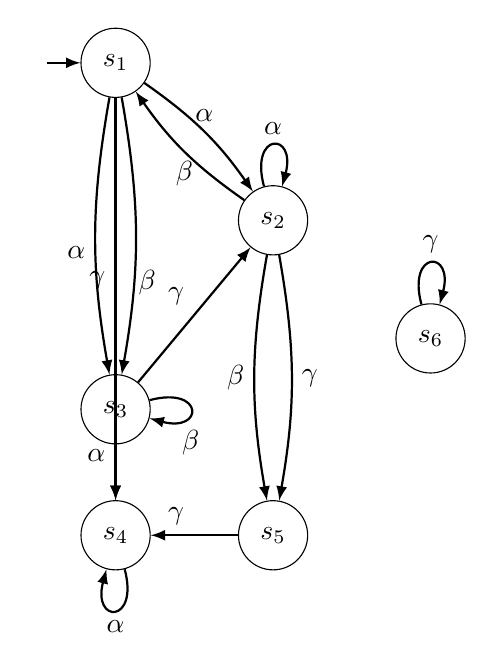
\begin{tikzpicture} [scale=2, every initial by arrow/.style={thick}]
		

		\path
		(\basex,		\basey) 		node[state,init] (s1) 	{$\state_1$} 
		(\basex+2,		\basey+0) 		node[state] (s2) 	{$\state_2$} 
		(\basex+1,		\basey-1.2) 	node[state] (s3) 	{$\state_3$} 
		(\basex,		\basey-2) 		node[state] (s4) 	{$\state_4$} 
		(\basex+2,		\basey-2) 		node[state] (s5) 	{$\state_5$}
		(\basex+3,		\basey-.75) 	node[state] (s6) 	{$\state_6$}
				
		;
		
%		
		\path [bendtrans] 	(s1) 	edge node [midway,above]				{\action} 		(s2);
		\path [bendtrans] 	(s1) 	edge node [near end,above right=-2pt]	{\actionb} 		(s3);
		\path [bendtransr] 	(s1) 	edge node [midway,below left]	{\action} 		(s3);
		\path [trans] 		(s1) 	edge node [midway,above left]	{\actionc} 		(s4);
		\path [bendtrans] 	(s2) 	edge node [midway,below]		{\actionb} 		(s1);
		\path [bendtransr] 	(s2) 	edge node [midway,left]			{\actionb} 		(s5);
		\path [bendtrans] 	(s2) 	edge node [midway,right]		{\actionc} 		(s5);
		\path [trans] 		(s3)	edge node [midway,above left]	{\actionc} 		(s2);
		\path [trans] 		(s3)	edge node [midway,above left]	{\action} 		(s4);
		\path [trans] 		(s5)	edge node [midway,above left]	{\actionc} 		(s4);
		
		\path [trans] 		(s2) 	edge [loop above] node [midway,above] {\action} 	(s2);
		\path [trans] 		(s3) 	edge [loop right] node [midway,below=4pt] {\actionb} 	(s3);
		\path [trans] 		(s4) 	edge [loop below] node [midway,below] {\action} 	(s4);
		\path [trans] 		(s6) 	edge [loop above] node [midway,above] {\actionc} 	(s6);
		
		
		%		midway, at start, near start, very near start, at end, near end, very near end
		
		
	\end{tikzpicture}
\end{document}
	\end{minipage}%
	\begin{minipage}{.5\textwidth}		
		\hspace{5mm}
		\documentclass[tikz,preview]{standalone}
%\usepackage{prelude}

%%%%%%%%%%%%%%%%%%%%%%%%%%%%%%%%%%%% PACKAGES %%%%%%%%%%%%%%%%%%%%%%%%%%%%%%%%%%%%%%%%%%

\usepackage{inputenc,fontenc}
\usepackage[a4paper,margin=3cm]{geometry}
\usepackage[english]{babel}
%\usepackage[german]{babel}
%\usepackage[fixlanguage]{babelbib}


\usepackage{bbold}
\usepackage{amsthm}
\usepackage{amsmath}
\usepackage{amssymb} % doteqdot
\usepackage[dvipsnames]{xcolor}
\usepackage{standalone}
\usepackage{tikz}[mode=buildnew]
\usepackage{cite}
\usepackage{xspace}
\usepackage{relsize}
\usepackage{mathtools} % mathclap
%\usepackage{MnSymbol}
\usepackage{hyperref}
\usepackage{url}
\usepackage{listings} % for code
\usepackage[T1]{fontenc} %<
\hypersetup{
	colorlinks,
	citecolor=black,
	filecolor=black,
	linkcolor=black,
	urlcolor=black
}
\usepackage{pgfplots}
\pgfplotsset{compat=1.18}
%\usepackage{courier} %% Sets font for listing as Courier. But also for url and texttt!
\usepackage{listings, xcolor}
\usepackage{graphicx}
\usepackage{subcaption}

\usetikzlibrary{calc}
%\usepackage{xparse} % \newDocumentCommand for multiple optional arguments
%\usepackage{titlecaps}



%%%%%%%%%%%%%%%%%%%%%%%%%%%%%%%%%%%% THEOREMSTYLES %%%%%%%%%%%%%%%%%%%%%%%%%%%%%%%%%%

\theoremstyle{definition}
\newtheorem{definition}{Definition}[section]
\newtheorem{exmp}{Beispiel}[section]
%\AfterEndEnvironment{definition}{\noindent\ignorespaces}

\theoremstyle{theorem}
\newtheorem{theorem}{Satz}[section]
\newtheorem{proposition}{Proposition}[section]
%\AfterEndEnvironment{theorem}{\noindent\ignorespaces}

\theoremstyle{korollary}
\newtheorem{korollary}{Korollar}[section]
%\AfterEndEnvironment{korollary}{\noindent\ignorespaces}


\tikzset{
	mstate/.style={draw, circle, minimum size=.94cm}, 
	gstate/.style={draw, rectangle, minimum size=.8cm},
	varstate/.style={draw,rectangle, rounded corners, minimum size=1}, 
	trans/.style={draw, ->, thick},
	bendtrans/.style={draw, ->, thick, bend left=10},
	bendtransr/.style={draw, ->, thick, bend right=10},
	init/.style={initial, initial distance=6pt, initial text=},
	every loop/.style={min distance=5pt, looseness=8},
	>=latex
}
\usetikzlibrary{automata,positioning}

%auto shift/.style={auto=right,->,
%	to path={ let \p1=(\tikztostart),\p2=(\tikztotarget),
%		\n1={atan2(\y2-\y1,\x2-\x1)},\n2={\n1+180}
%		in ($(\tikztostart.{\n1})!1mm!270:(\tikztotarget.{\n2})$) -- 
%		($(\tikztotarget.{\n2})!1mm!90:(\tikztostart.{\n1})$) \tikztonodes}},

%%%%%%%%%%%%%%%%%%%%%%%%%%%%%%%%%%% MY MACROS %%%%%%%%%%%%%%%%%%%%%%%%%%%%%%%%%%%%%%%%%
%formatting
\newcommand{\comment}[2]{{\color{#1}#2}}
\newcommand{\redcomment}[1]{{\color{red}#1}}
\newcommand{\purpcomment}[1]{{\color{pink}#1}}
\newcommand{\bluecomment}[1]{{\color{blue}#1}}
\newcommand{\mt}[1]{\ensuremath{{#1}}\xspace}
\newcommand{\mynewcommand}[2]{\newcommand{#1}{\mt{#2}}} %% currently not used becaue of ide highlighting
\newcommand{\arr}{\mt{\to}}

%model checking terms
\newcommand{\mimicrel}{\mt{\mathcal{R}}}
\newcommand{\bisimeq}{\mt{\;\!\sim\;\!}}
\newcommand{\simorder}{\mt{\;\!\preceq\;\!}}
\newcommand{\simequiv}{\mt{\;\!\simeq\;\!}} %command already defined
\newcommand{\relts}{\mt{\;\!\bullet_{_{\tiny{TS}}}\;\!}}
\newcommand{\rel}{\mt{\;\!\bullet\;\!}}

%own names
\newcommand{\nm}[1]{#1\xspace}
\newcommand{\mdpN}{\nm{MDP}}
\newcommand{\mdpsN}{\nm{MDPs}}
\newcommand{\viewN}{\nm{view}}
\newcommand{\viewNC}{\nm{View}}
\newcommand{\viewsN}{\nm{views}}
\newcommand{\viewsNC}{\nm{Views}}
\newcommand{\grpfctsubN}{\nm{detached grouping function}}
\newcommand{\grpfctsubNC}{\nm{detached grouping function}}
\newcommand{\grpfctsubNCC}{\nm{Detached Grouping Function}}
\newcommand{\grpfctN}{\nm{grouping function}}
\newcommand{\grpfctNC}{\nm{Grouping function}}
\newcommand{\grpfctNCC}{\nm{Grouping Function}}
\newcommand{\grpfctsN}{\nm{grouping functions}}
\newcommand{\grpfctsNC}{\nm{Grouping functions}}
\newcommand{\grpfctsNCC}{\nm{Grouping Functions}}
\newcommand{\stmimicN}{\nm{state-mimic}}
\newcommand{\stmimicsN}{\nm{state-mimics}}
\newcommand{\stmimickingN}{\nm{state-mimicking}}
\newcommand{\stmimickedN}{\nm{state-mimicked}}
%\newcommand{\chosenphtypeNCC}{\nm{Transition System}}
%\newcommand{\chgphNC}{\nm{Transition system}}
%\newcommand{\chgphN}{\nm{transition system}}
%\newcommand{\chgphsNCC}{\nm{Transition Systems}}
%\newcommand{\chgphsNC}{\nm{Transition systems}}
%\newcommand{\chgphsN}{\nm{transition systems}}
\newcommand{\chgphNCC}{\nm{MDP}}
\newcommand{\chgphNC}{\nm{MDP}}
\newcommand{\chgphN}{\nm{MDP}}
\newcommand{\achgphN}{\nm{an MDP}}
\newcommand{\chgphsNCC}{\nm{MDPs}}
\newcommand{\chgphsNC}{\nm{MDPs}}
\newcommand{\chgphsN}{\nm{MDPs}}
\newcommand{\parllcompN}{\nm{parallel composition}}
\newcommand{\parllcompNC}{\nm{Parallel composition}}
\newcommand{\parllcompNCC}{\nm{Parallel Composition}}
\newcommand{\parllcompsN}{\nm{parallel compositions}}
\newcommand{\parllcompsNC}{\nm{Parallel compositions}}
\newcommand{\parllcompsNCC}{\nm{Parallel Compositions}}
\newcommand{\sccN}{\nm{SCC}}
\newcommand{\sccsN}{\nm{SCCs}}
\newcommand{\bsccN}{\nm{BSCC}}
\newcommand{\bsccsN}{\nm{BSCCs}}
\newcommand{\jgrapht}{\nm{jGraphtT}}

\newcommand{\outactident}{\nm{OutActionsIdent}}

%names
\newcommand{\iffN}{\nm{if and only if}}
\newcommand{\tsN}{\nm{TS}}

%% outactions identical
\newcommand{\outactidentstrong}{\nm{strong}}
\newcommand{\outactidentweak}{\nm{weak}}

% CORE DEFINITIONS
\newcommand{\grpfct}[1][\viewppty]{\mt{F_{#1}}}
\newcommand{\grpfctsub}[1][\viewppty]{\mt{\tilde{F}_{#1}}}
%\newcommand{\grpfctimg}[1]{\mt{{\grpfct}[{#1}]}}
%\newcommand{\fctimg}[2]{\mt{{#1}[{#2}]}}
\newcommand{\eqrelview}{\mt{R}}
\newcommand{\eqclassv}[1][\state]{\mt{\eqclass{#1}{\eqrelview}}}
\newcommand{\eqclasssetv}[1][\states]{\mt{{#1}/\eqrelview}} %OLD: \bigcup_{\state \in \states} \eqclassv
\newcommand{\viewid}{\mt{\mdp}}
\newcommand{\view}[1][\viewppty]{\mt{\viewid_{#1}}}
\newcommand{\imggrp}{\mt{\arbset}}
\newcommand{\imggrpsub}{\mt{X}}
\newcommand{\viewppty}{\mt{\theta}}
\newcommand{\pll}{\mt{\;\!\pllpure\;\!}}
\newcommand{\pllrev}{\mt{\pllpure^{-1}}}
\newcommand{\pllpure}{\mt{||}}
\newcommand{\compselectset}{\mt{Z}}
\newcommand{\compselectpure}{\mt{\pllpure_\compselectset}}
\newcommand{\compselect}{\mt{\;\pllpure_\compselectset\;}}
\newcommand{\remstates}{\mt{\bigcup_{\state \in \states \setminus \states_1}\{\{\state\}\}}}
\newcommand{\nogroupstates}[1][\states_2]{\mt{\bigcup_{\state \in \states \setminus {#1}}\{\{\state\}\}}}
\newcommand{\remelem}{\mt{\bullet}}
\newcommand{\nogroupset}{\mt{\xi}}
\newcommand{\remset}{\mt{\{\remelem\}}}
\newcommand{\gfctpll}{\mt{\grpfct[\pll]}}
\newcommand{\group}{\mt{\top}}
\newcommand{\imggrpbinview}{\mt{\{\remelem, \notppty\}}}
\newcommand{\viewappset}{\mt{\tilde{\states}}}
\newcommand{\hasppty}{\mt{\top}}
\newcommand{\notppty}{\mt{\bot}}
\newcommand{\disregardelem}{\mt{\Delta}}
\newcommand{\disregardelements}{\mt{{\disregardelem_1, \dots, \disregardelem_n}}}



%\newcommand{\mdp}{def}\mdp
%\newcommand{\mdpdef}



% EXAMPLE VIEWS
\newcommand{\pptyatomicprops}{\mt{\atomicprops}}
\newcommand{\pptyinitstates}{\mt{\initstates}}
\newcommand{\pptyinactsetsize}{\mt{|\inacts(\state)|}}
\newcommand{\pptyhasoutact}{\mt{\exists\outact}}
\newcommand{\pptyminoutact}[2]{\mt{#1\leq#2}}
\newcommand{\pptymaxoutact}[2]{\mt{#2\leq#1}}
\newcommand{\pptyspanoutact}[3]{\mt{#1\leq#2\leq#3}}
\newcommand{\pptyoutactsetsize}{\mt{|\outacts(\state)|}}
\newcommand{\pptyoutactsingle}{\mt{|\outacts(\state)|_1}}
\newcommand{\pptystrongoutactident}{\mt{\outacts(\state)_=}}
\newcommand{\pptyweakoutactident}{\mt{\outacts(\state)_\approx}}
\newcommand{\pptyhasinact}{\mt{\exists\inact}}
\newcommand{\pptymininact}[2]{\mt{#1\leq#2}}
\newcommand{\pptymaxinact}[2]{\mt{#2\leq#1}}
\newcommand{\pptyspaninact}[3]{\mt{#1\leq#2\leq#3}}
\newcommand{\pptyinactsingle}{\mt{|\inacts(\state)|_1}}
\newcommand{\pptystronginactident}{\mt{\inacts(\state)_=}}
\newcommand{\pptyweakinactident}{\mt{\inacts(\state)_\approx}}
\newcommand{\pptyparamvalueseq}{\mt{\var = \varval}}
\newcommand{\pptyparamvaluesneq}{\mt{\var \neq \varval}}
\newcommand{\pptyparamdnf}{\mt{VarDNF}}
\newcommand{\pptyparamcnf}{\mt{VarCNF}}
\newcommand{\pptyparamvalueseqopt}{\mt{\var = \varval}}
\newcommand{\pptyparamvalident}{\mt{Var:\varval}}
\newcommand{\pptydistance}{\mt{\distpath}}
\newcommand{\pptydistancerev}{\mt{\distpathrev}}
\newcommand{\pptydistancebi}{\mt{\distpathbi}}
\newcommand{\pptyhascycle}{\mt{\exists\cycle}}
\newcommand{\pptyexactactcycle}{\mt{\{\cycle_{\action,n}\}}}
\newcommand{\pptycycleset}{\mt{\cup{\{\state\}_\cycle}}}
\newcommand{\pptyexactcycle}{\mt{\{\cycle_n\}}}
\newcommand{\pptyscc}{\mt{scc}}
\newcommand{\pptybscc}{\mt{bscc}}
\newcommand{\pptyprop}{\mt{\redcomment{?}}}
\newcommand{\pptyident}{id}


\newcommand{\gfctatomicprops}{\mt{\grpfct[\pptyatomicprops]}}
\newcommand{\gfctinitstates}{\mt{\grpfct[\pptyinitstates]^\hasppty}}
\newcommand{\gfcthasoutaction}{\mt{\grpfct[\pptyhasoutact]^\hasppty}}
\newcommand{\gfctminoutaction}{\mt{\grpfct[\pptyminoutact{\numoutact}{\outact}]^\hasppty}}
\newcommand{\gfctmaxoutaction}{\mt{\grpfct[\pptymaxoutact{\numoutact}{\outact}]^\hasppty}}
\newcommand{\gfctspanoutaction}{\mt{\grpfct[\pptyspanoutact{\numoutactb}{\outact}{\numoutact}]^\hasppty}}
\newcommand{\gfctoutactsetsize}{\mt{\grpfct[\pptyoutactsetsize]}}
\newcommand{\gfctoutactsingle}{\mt{\grpfct[\pptyoutactsingle]^\notppty}}
\newcommand{\gfctstrongoutactident}{\mt{\grpfct[\pptystrongoutactident]}}
\newcommand{\gfctweakoutactident}{\mt{\grpfct[\pptyweakoutactident]}}
\newcommand{\gfcthasinaction}{\mt{\grpfct[\pptyhasinact]^\hasppty}}
\newcommand{\gfctmininaction}{\mt{\grpfct[\pptymininact{\numinact}{\inact}]^\hasppty}}
\newcommand{\gfctmaxinaction}{\mt{\grpfct[\pptymaxinact{\numinact}{\inact}]^\hasppty}}
\newcommand{\gfctspaninaction}{\mt{\grpfct[\pptyspaninact{\numinactb}{\inact}{\numinact}]^\hasppty}}
\newcommand{\gfctinactsetsize}{\mt{\grpfct[\pptyinactsetsize]}}
\newcommand{\gfctinactsingle}{\mt{\grpfct[\pptyinactsingle]^\notppty}}
\newcommand{\gfctstronginactident}{\mt{\grpfct[\pptystronginactident]}}
\newcommand{\gfctweakinactident}{\mt{\grpfct[\pptyweakinactident]}}
\newcommand{\gfctparamvalueseq}{\mt{\grpfct[\pptyparamvalueseq]^\hasppty}}
\newcommand{\gfctparamvaluesneq}{\mt{\grpfct[\pptyparamvaluesneq]^\hasppty}}
\newcommand{\gfctparamdnf}{\mt{\grpfct[\pptyparamdnf]^\hasppty}}
\newcommand{\gfctparamcnf}{\mt{\grpfct[\pptyparamcnf]^\hasppty}}
\newcommand{\gfctparamvalueseqopt}{\mt{\pptyparamvalueseqopt}}
\newcommand{\gfctparamvalident}{\mt{\grpfct[\pptyparamvalident]}}
\newcommand{\gfctdistance}{\mt{\grpfct[\pptydistance]}}
\newcommand{\gfctdistancerev}{\mt{\grpfct[\pptydistancerev]}}
\newcommand{\gfctdistancebi}{\mt{\grpfct[\pptydistancebi]}}
\newcommand{\gfcthascycle}{\mt{\grpfct[\pptyhascycle]}}
\newcommand{\gfctexactcycle}{\mt{\grpfct[\pptyexactcycle]}}
\newcommand{\gfctcycleset}{\mt{\grpfct[\pptycycleset]}}
\newcommand{\gfctexactactcycle}{\mt{\grpfct[\pptyexactactcycle]}}
\newcommand{\gfctscc}{\mt{\grpfct[\pptyscc]}}
\newcommand{\gfctbscc}{\mt{\grpfct[\pptybscc]}}
\newcommand{\gfctprop}{\mt{\grpfct[\pptyprop]}}
\newcommand{\gfctident}{\mt{\grpfct[\pptyident]}}

\newcommand{\gfctsubatomicprops}{\mt{\grpfctsub[\pptyatomicprops]}}
\newcommand{\gfctsubinitstates}{\mt{\grpfctsub[\pptyinitstates]^\hasppty}}
\newcommand{\gfctsubhasoutaction}{\mt{\grpfctsub[\pptyhasoutact]^\hasppty}}
\newcommand{\gfctsubminoutaction}{\mt{\grpfctsub[\pptyminoutact{\numoutact}{\outact}]^\hasppty}}
\newcommand{\gfctsubmaxoutaction}{\mt{\grpfctsub[\pptymaxoutact{\numoutact}{\outact}]^\hasppty}}
\newcommand{\gfctsubspanoutaction}{\mt{\grpfctsub[\pptyspanoutact{\numoutactb}{\outact}{\numoutact}]^\hasppty}}
\newcommand{\gfctsuboutactsetsize}{\mt{\grpfctsub[\pptyoutactsetsize]}}
\newcommand{\gfctsuboutactsingle}{\mt{\grpfctsub[\pptyoutactsingle]^\notppty}}
\newcommand{\gfctsubstrongoutactident}{\mt{\grpfctsub[\pptystrongoutactident]^\hasppty}}
\newcommand{\gfctsubweakoutactident}{\mt{\grpfctsub[\pptyweakoutactident]^\hasppty}}
\newcommand{\gfctsubhasinaction}{\mt{\grpfctsub[\pptyhasinact]}}
\newcommand{\gfctsubmininaction}{\mt{\grpfctsub[\pptymininact{\numinact}{\inact}]}}
\newcommand{\gfctsubmaxinaction}{\mt{\grpfctsub[\pptymaxinact{\numinact}{\inact}]}}
\newcommand{\gfctsubspaninaction}{\mt{\grpfctsub[\pptyspaninact{\numinactb}{\inact}{\numinact}]}}
\newcommand{\gfctsubinactsetsize}{\mt{\grpfctsub[\pptyinactsetsize]^\hasppty}}
\newcommand{\gfctsubinactsingle}{\mt{\grpfctsub[\pptyinactsingle]^\notppty}}
\newcommand{\gfctsubstronginactident}{\mt{\grpfctsub[\pptystronginactident]}}
\newcommand{\gfctsubweakinactident}{\mt{\grpfctsub[\pptyweakinactident]}}
\newcommand{\gfctsubparamvalueseq}{\mt{\grpfctsub[\pptyparamvalueseq]^\hasppty}}
\newcommand{\gfctsubparamvaluesneq}{\mt{\grpfctsub[\pptyparamvaluesneq]^\hasppty}}
\newcommand{\gfctsubparamdnf}{\mt{\grpfctsub[\pptyparamdnf]^\hasppty}}
\newcommand{\gfctsubparamcnf}{\mt{\grpfctsub[\pptyparamcnf]^\hasppty}}
\newcommand{\gfctsubparamvalueseqopt}{\mt{\pptyparamvalueseqopt}}
\newcommand{\gfctsubparamvalident}{\mt{\grpfctsub[\pptyparamvalident]}}
\newcommand{\gfctsubdistance}{\mt{\grpfctsub[\pptydistance]}}
\newcommand{\gfctsubdistancerev}{\mt{\grpfctsub[\pptydistancerev]}}
\newcommand{\gfctsubdistancebi}{\mt{\grpfctsub[\pptydistancebi]}}
\newcommand{\gfctsubhascycle}{\mt{\grpfctsub[\pptyhascycle]^\hasppty}}
\newcommand{\gfctsubexactcycle}{\mt{\grpfctsub[\pptyexactcycle]}}
\newcommand{\gfctsubcycleset}{\mt{\grpfctsub[\pptycycleset]}}
\newcommand{\gfctsubexactactcycle}{\mt{\grpfctsub[\pptyexactactcycle]}}
\newcommand{\gfctsubscc}{\mt{\grpfctsub[\pptyscc]}}
\newcommand{\gfctsubbscc}{\mt{\grpfctsub[\pptybscc]}}
\newcommand{\gfctsubprop}{\mt{\grpfctsub[\pptyprop]}}
\newcommand{\gfctsubident}{\mt{\grpfctsub[\pptyident]}}


\newcommand{\viewatomicprops}{\mt{\view[\pptyatomicprops]}}
\newcommand{\viewinitstates}{\mt{\view[\pptyinitstates]^\hasppty}}
\newcommand{\viewhasoutaction}{\mt{\view[\pptyhasoutact]^\hasppty}}
\newcommand{\viewminoutaction}{\mt{\view[\pptyminoutact{\numoutact}{\outact}]^\hasppty}}
\newcommand{\viewmaxoutaction}{\mt{\view[\pptymaxoutact{\numoutact}{\outact}]^\hasppty}}
\newcommand{\viewspanoutaction}{\mt{\view[\pptyspanoutact{\numoutactb}{\outact}{\numoutact}]^\hasppty}}
\newcommand{\viewoutactsetsize}{\mt{\view[\pptyoutactsetsize]}}
\newcommand{\viewoutactsingle}{\mt{\view[\pptyoutactsingle]^\notppty}}
\newcommand{\viewstrongoutactident}{\mt{\view[\pptystrongoutactident]}}
\newcommand{\viewweakoutactident}{\mt{\view[\pptyweakoutactident]}}
\newcommand{\viewhasinaction}{\mt{\view[\pptyhasinact]^\hasppty}}
\newcommand{\viewmininaction}{\mt{\view[\pptymininact{\numinact}{\inact}]^\hasppty}}
\newcommand{\viewmaxinaction}{\mt{\view[\pptymaxinact{\numinact}{\inact}]^\hasppty}}
\newcommand{\viewspaninaction}{\mt{\view[\pptyspaninact{\numinactb}{\inact}{\numinact}]^\hasppty}}
\newcommand{\viewinactsetsize}{\mt{\view[\pptyinactsetsize]}}
\newcommand{\viewinactsingle}{\mt{\view[\pptyinactsingle]^\notppty}}
\newcommand{\viewstronginactident}{\mt{\view[\pptystronginactident]}}
\newcommand{\viewweakinactident}{\mt{\view[\pptyweakinactident]}}
\newcommand{\viewparamvalueseq}{\mt{\view[\pptyparamvalueseq]}}
\newcommand{\viewparamvaluesneq}{\mt{\view[\pptyparamvaluesneq]}}
\newcommand{\viewparamdnf}{\mt{\view[\pptyparamdnf]^\hasppty}}
\newcommand{\viewparamcnf}{\mt{\view[\pptyparamcnf]^\hasppty}}
\newcommand{\viewparamvalueseqopt}{\mt{\pptyparamvalueseqopt}}
\newcommand{\viewparamvalident}{\mt{\view[\pptyparamvalident]}}
\newcommand{\viewdistance}{\mt{\view[\pptydistance]}}
\newcommand{\viewdistancerev}{\mt{\view[\pptydistancerev]}}
\newcommand{\viewdistancebi}{\mt{\view[\pptydistancebi]}}
\newcommand{\viewhascycle}{\mt{\view[\pptyhascycle]}}
\newcommand{\viewexactcycle}{\mt{\view[\pptyexactcycle]}}
\newcommand{\viewcycleset}{\mt{\view[\pptycycleset]}}
\newcommand{\viewexactactcycle}{\mt{\view[\pptyexactactcycle]}}
\newcommand{\viewscc}{\mt{\view[\pptyscc]}}
\newcommand{\viewbscc}{\mt{\view[\pptybscc]}}
\newcommand{\viewprop}{\mt{\view[\pptyprop]}}
\newcommand{\viewident}{\mt{\view[\pptyident]}}

%\newcommand{\viewatomicprops}{\mt{\view[\atomicprops]}}
%\newcommand{\viewinitstates}{\mt{\view[\initstates]}}
%\newcommand{\viewhasoutaction}{\mt{\view[\pptyhasoutact]}}
%\newcommand{\viewminoutaction}{\mt{\view[\pptyminoutact{\numoutact}{\outact}]}}
%\newcommand{\viewmaxoutaction}{\mt{\view[\pptymaxoutact{\numoutact}{\outact}]}}
%\newcommand{\viewspanoutaction}{\mt{\view[\pptyspanoutact{\numoutactb}{\outact}{\numoutact}]}}
%\newcommand{\viewoutactsetsize}{\mt{\view[\pptyoutactsetsize]}}
%\newcommand{\viewoutactsingle}{\mt{\view[\pptyoutactsingle]}}
%\newcommand{\viewstrongoutactident}{\mt{\view[\outacts(\state)_=]}}
%\newcommand{\viewweakoutactident}{\mt{\view[\outacts(\state)_\approx]}}
%\newcommand{\viewhasinaction}{\mt{\view[\pptyhasinact]}}
%\newcommand{\viewmininaction}{\mt{\view[\pptymininact{\numinact}{\inact}]}}
%\newcommand{\viewmaxinaction}{\mt{\view[\pptymaxinact{\numinact}{\inact}]}}
%\newcommand{\viewspaninaction}{\mt{\view[\pptyspaninact{\numinactb}{\inact}{\numinact}]}}
%\newcommand{\viewinactsetsize}{\mt{\view[\pptyinactsetsize]}}
%\newcommand{\viewinactsingle}{\mt{\view[\pptyinactsingle]}}
%\newcommand{\viewstronginactident}{\mt{\view[\inacts(\state)_=]}}
%\newcommand{\viewweakinactident}{\mt{\view[\inacts(\state)_\approx]}}
%\newcommand{\viewparamvalueseq}{\mt{\view[\var = \varval]}}
%\newcommand{\viewparamvaluesneq}{\mt{\view[\var \neq \varval]}}
%\newcommand{\viewparamdnf}{\mt{\view[VarDNF]}}
%\newcommand{\viewparamcnf}{\mt{\view[VarCNF]}}
%\newcommand{\viewparamvalident}{\mt{\view[\pptyparamvalident]}}
%\newcommand{\viewdistance}{\mt{\view[\pptydistance]}}
%\newcommand{\viewhascycle}{\mt{\view[\exists\cycle]}}
%\newcommand{\viewexactcycle}{\mt{\view[\pptyexactcycle]}}
%\newcommand{\viewcycleset}{\mt{\view[\pptycycleset]}}
%\newcommand{\viewexactactcycle}{\mt{\view[\pptyexactactcycle]}}
%\newcommand{\viewscc}{\mt{\view[scc]}}
%\newcommand{\viewbscc}{\mt{\view[bscc]}}

%actions
\newcommand{\numoutact}{\mt{n}}
\newcommand{\numoutactb}{\mt{m}}
\newcommand{\numinact}{\mt{n}}
\newcommand{\numinactb}{\mt{m}}

\newcommand{\predmaxoutact}[1][\numoutact]{\mt{Q_{\outact\leq#1}(\state,\state_1, \dots, \state_{#1+1})}}
\newcommand{\predminoutact}[1][\numoutact]{\mt{Q_{#1\leq\outact}(\state,\state_1, \dots, \state_{#1})}}
\newcommand{\formoutact}[1][\state]{\mt{C_{#1,\outact}}}
\newcommand{\predmaxinact}[1][\numinact]{\mt{Q_{\inact\leq#1}(\state,\state_1, \dots, \state_{#1+1})}}
\newcommand{\predmininact}[1][\numinact]{\mt{Q_{#1\leq\inact}(\state,\state_1, \dots, \state_{#1})}}

\newcommand{\outact}[1][\action]{\mt{\overrightarrow{#1}}}
\newcommand{\outacts}{\mt{\overrightarrow{\actions}}}
\newcommand{\inact}{\mt{\overleftarrow{\action}}}
\newcommand{\inacts}[1][\action]{\mt{\overleftarrow{#1}}}

%%Parameters
\newcommand{\vars}[1][\mdp]{\mt{V\!ar_{#1}}}
\newcommand{\var}{\mt{x}}
\newcommand{\varstate}[1][]{\mt{\var_{\state#1}}}
\newcommand{\varval}{\mt{a}}
\newcommand{\vareval}[1][\mdp]{\mt{V\!arEval_{#1}}}
\newcommand{\varevalimg}[1][\mdp]{\mt{\vareval[#1][\states,\vars]}}
\newcommand{\varevalimgset}{\mt{\arbset}}
\newcommand{\someparam}{\mt{\tilde{x}}}
\newcommand{\eqorneq}{\mt{\;\doteqdot\;}}
\newcommand{\varstyle}[2]{\mt{\langle#1,#2\rangle}}




%\makeatletter
%\newcommand{\overleftrightsmallarrow}{\mathpalette{\overarrowsmall@\leftrightarrowfill@}}
%\newcommand{\overrightsmallarrow}{\mathpalette{\overarrowsmall@\rightarrowfill@}}
%\newcommand{\overleftsmallarrow}{\mathpalette{\overarrowsmall@\leftarrowfill@}}
%\newcommand{\overarrowsmall@}[3]{%
%	\vbox{%
%		\ialign{%
%			##\crcr
%			#1{\smaller@style{#2}}\crcr
%			\noalign{\nointerlineskip}%
%			$\m@th\hfil#2#3\hfil$\crcr
%		}%
%	}%
%}
%\def\smaller@style#1{%
%	\ifx#1\displaystyle\scriptstyle\else
%	\ifx#1\textstyle\scriptstyle\else
%	\scriptscriptstyle
%	\fi
%	\fi
%}
%\makeatother
%\newcommand{\te}[1]{\overleftrightsmallarrow{#1}}

% Distance
\newcommand{\fctdist}{\mt{distance}}
\newcommand{\fctdistdefault}{\mt{\fctdist(\chgph, \smstates, \grandist)}}
\newcommand{\distval}{\mt{d}}
\newcommand{\grandist}{\mt{n}}
\let\path\oldpath
\newcommand{\path}{\mt{P}}
\newcommand{\pathbi}{\mt{\bar{\path}}}
\newcommand{\pathsecfull}{\mt{(\state_0, \action_0, \state_1, \action_1, \dots, \action_{n}, \state_{n+1})}}
\newcommand{\lenpath}{\mt{len}}
\newcommand{\pfirst}{\mt{first}}
\newcommand{\plast}{\mt{last}}
\newcommand{\pathset}{\mt{\path_\chgph}}
\newcommand{\pathbiset}{\mt{\pathbi_\chgph}}
\newcommand{\distpath}{\mt{\overrightarrow{dist}}}
\newcommand{\distpathrev}{\mt{\overleftarrow{dist}}}
\newcommand{\distpathbi}{\mt{\overline{dist}}}
%Cycles
\newcommand{\cyclesecfull}{\mt{(\state_0, \action_0, \state_1, \action_1, \dots, \action_{n-1}, \state_0)}}
\newcommand{\fctfindcycles}{\mt{findCycles}}
\newcommand{\cycle}{\mt{C}}
\newcommand{\cycleset}{\mt{\cycle_{\mdp, n}}}
\newcommand{\lencycle}{\mt{len}}
% strongly connected components
\newcommand{\scc}{\mt{T}}
\newcommand{\setscc}{\mt{SCC_{\chgph,n}}}
\newcommand{\setbscc}{\mt{BSCC_{\chgph,n}}}

% properties
\newcommand{\propfct}{\mt{f}}

% all Systems
\newcommand{\chgph}{\mt{\mdp}}
\newcommand{\chgphtuple}{\mt{\mdptuple}}
\newcommand{\chgphtupledist}{\mt{\mdptupledist}}

\newcommand{\states}{\mt{S}}
\newcommand{\actions}{\mt{Act}}
\newcommand{\atomicprops}{\mt{AP}}
\newcommand{\labelingfct}{\mt{L}}
\newcommand{\init}{\mt{\initdistrib}} % use MDP % refers to the underlying set
\newcommand{\trans}{\mt{\probtfunc}} % use MDP % refers to the underlying set
\newcommand{\smstates}{\mt{\tilde{\states}}}


\newcommand{\state}{\mt{s}}
\newcommand{\action}{\mt{\alpha}}
\newcommand{\actionb}{\mt{\beta}}
\newcommand{\actionc}{\mt{\gamma}}
\newcommand{\smstate}{\mt{\tilde{\state}}}



% transition sysstems
\newcommand{\ts}{\mt{TS}}
\newcommand{\transitionrel}{\mt{\longrightarrow}}
\newcommand{\initstates}{\mt{I}}
\newcommand{\transitionsystem}{\mt
	{(\states, \actions, \transitionrel, \initstates, \atomicprops, \labelingfct)}
}
\newcommand{\tstupledist}{\mt{(\states', \actions',\transitionrel', \initstates', \labelingfct')}}


%Markov chains and MDP
\newcommand{\mdp}{\mt{\autm}}
\newcommand{\mdptuple}{\mt{(\states, \actions, \probtfunc, \initdistrib, \atomicprops, \labelingfct)}}
\newcommand{\mdptupledist}{\mt{(\states', \actions', \probtfunc', \initdistrib', \atomicprops', \labelingfct')}}
\newcommand{\autm}{\mt{\mathcal{M}}}
\newcommand{\probtfunc}{\mt{\textbf{P}}}
\newcommand{\initdistrib}{\mt{\iota_{init}}}


%maths
\newcommand{\powerset}[1]{\mt{\mathcal{P}(#1)}}
\newcommand{\eqclass}[2]{\mt{[#1]_{#2}}}%{\mt{#1 / #2}}
\newcommand{\impr}{\mt{\hspace{3mm}\Rightarrow\hspace{2mm}}}
\newcommand{\impl}{\mt{\hspace{3mm}\Leftarrow\hspace{2mm}}}
\newcommand{\natnums}{\mt{\mathbb{N}}} 
\newcommand{\realnums}{\mt{\mathbb{R}}}
\newcommand{\intmodn}[1][n]{\mt{\mathbb{Z}_{#1}}}
\newcommand{\arbset}{\mt{M}}
\newcommand{\bigsum}[2][]{\mt{\mathlarger{\sum}_{#2}^{#1}}}
\newcommand{\bbigsum}[2][]{\mt{\mathlarger{\mathlarger{\sum}}_{#2}^{#1}}}
\newcommand{\invimage}[2]{#1^{\mt{-1}(#2)}}
\newcommand{\img}{\mt{Img}}
\newcommand{\cond}{\mt{\,|\,}}

%tickz
%% \definecolor{darkred}{RGB}{196, 42, 42}

%implementation
\newcommand{\pmcvis}{\nm{PMC-Vis}}





\begin{document}
	\newcommand{\basex}{0}
	\newcommand{\basey}{0}
	\newcommand{\createstate}[3]{\node[draw, circle, minimum size=1cm] (#1) at (#2) {#3}}
	
	
	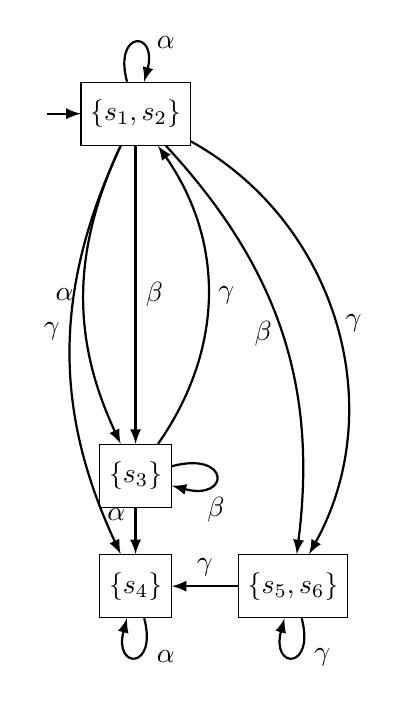
\begin{tikzpicture} [scale=2, every initial by arrow/.style={thick}]
		
		
%	\path
%	(\basex+1,		\basey) 		node[gstate,init, initial left] (s12) 	{$\state_1, \state_2$} 
%	(\basex+1,		\basey-1.3) 		node[gstate] (s3) 	{$\state_3$} 
%	(\basex,		\basey-2) 	node[gstate] (s4) 	{$\state_4$} 
%	(\basex+2,		\basey-2)		node[gstate] (s56) 	{$\state_5,\state_6$} 
%	
%	;
	\path
	(\basex+1,		\basey) 		node[gstate,init, initial left] (s12) 	{$\{\state_1, \state_2\}$} 
	(\basex+1,		\basey-1.3) 		node[gstate] (s3) 	{$\{\state_3\}$} 
	(\basex,		\basey-2) 	node[gstate] (s4) 	{$\{\state_4\}$} 
	(\basex+2,		\basey-2)		node[gstate] (s56) 	{$\{\state_5,\state_6\}$} 
	
	;
	
	\path [trans, bend right=25] 		(s12) 	edge node [midway,above left]		{\actionc} 		(s4);
	\path [trans] 		(s12) 	edge node [midway,right]			{\actionb} 		(s3);
	\path [trans, bend right=25] 		(s12) 	edge node [midway,left]				{\action} 		(s3);
	\path [trans, bend left=25](s12) 	edge node [midway,left]			{\actionb} 		(s56);
	\path [trans, bend left=45] (s12) 	edge node [midway,right]		{\actionc} 		(s56);
	\path [trans,bend right=35] 	(s3) 	edge node [midway,right]	{\actionc} 		(s12);
	\path [trans] 	(s3) 	edge node [midway,above left]	{\action} 		(s4);
	\path [trans] 	(s56) 	edge node [midway,above]	{\actionc} 		(s4);
	
%	\path [trans] 		(s12) 	edge [loop, in=15, out=50, looseness=6] node [midway,right] {\action,\actionb} 	(s12);
	\path [trans] 		(s12) 	edge [loop above] node [midway,right=4pt] {\action} 	(s12);
	\path [trans] 		(s3) 	edge [loop right] node [midway,below=4pt] {\actionb} 	(s3);
	\path [trans] 		(s4) 	edge [loop below] node [midway,right=4pt] {\action} 	(s4);
	\path [trans] 		(s56) 	edge [loop below] node [midway,right=4pt] {\actionc} 	(s56);
		
		
	\end{tikzpicture}
\end{document}
	\end{minipage}
	
	\caption{Simplified representations of \mdp (left) and the \viewN \viewstrongoutactident on it (right)}
	\label{fig:outActIdentStrongAfter}

\end{figure}

\begin{figure}[h]
	\begin{minipage}{.5\textwidth}
		\hspace{5mm}
		\documentclass[tikz,preview]{standalone}
%\usepackage{prelude}

%%%%%%%%%%%%%%%%%%%%%%%%%%%%%%%%%%%% PACKAGES %%%%%%%%%%%%%%%%%%%%%%%%%%%%%%%%%%%%%%%%%%

\usepackage{inputenc,fontenc}
\usepackage[a4paper,margin=3cm]{geometry}
\usepackage[english]{babel}
%\usepackage[german]{babel}
%\usepackage[fixlanguage]{babelbib}


\usepackage{bbold}
\usepackage{amsthm}
\usepackage{amsmath}
\usepackage{amssymb} % doteqdot
\usepackage[dvipsnames]{xcolor}
\usepackage{standalone}
\usepackage{tikz}[mode=buildnew]
\usepackage{cite}
\usepackage{xspace}
\usepackage{relsize}
\usepackage{mathtools} % mathclap
%\usepackage{MnSymbol}
\usepackage{hyperref}
\usepackage{url}
\usepackage{listings} % for code
\usepackage[T1]{fontenc} %<
\hypersetup{
	colorlinks,
	citecolor=black,
	filecolor=black,
	linkcolor=black,
	urlcolor=black
}
\usepackage{pgfplots}
\pgfplotsset{compat=1.18}
%\usepackage{courier} %% Sets font for listing as Courier. But also for url and texttt!
\usepackage{listings, xcolor}
\usepackage{graphicx}
\usepackage{subcaption}

\usetikzlibrary{calc}
%\usepackage{xparse} % \newDocumentCommand for multiple optional arguments
%\usepackage{titlecaps}



%%%%%%%%%%%%%%%%%%%%%%%%%%%%%%%%%%%% THEOREMSTYLES %%%%%%%%%%%%%%%%%%%%%%%%%%%%%%%%%%

\theoremstyle{definition}
\newtheorem{definition}{Definition}[section]
\newtheorem{exmp}{Beispiel}[section]
%\AfterEndEnvironment{definition}{\noindent\ignorespaces}

\theoremstyle{theorem}
\newtheorem{theorem}{Satz}[section]
\newtheorem{proposition}{Proposition}[section]
%\AfterEndEnvironment{theorem}{\noindent\ignorespaces}

\theoremstyle{korollary}
\newtheorem{korollary}{Korollar}[section]
%\AfterEndEnvironment{korollary}{\noindent\ignorespaces}


\tikzset{
	mstate/.style={draw, circle, minimum size=.94cm}, 
	gstate/.style={draw, rectangle, minimum size=.8cm},
	varstate/.style={draw,rectangle, rounded corners, minimum size=1}, 
	trans/.style={draw, ->, thick},
	bendtrans/.style={draw, ->, thick, bend left=10},
	bendtransr/.style={draw, ->, thick, bend right=10},
	init/.style={initial, initial distance=6pt, initial text=},
	every loop/.style={min distance=5pt, looseness=8},
	>=latex
}
\usetikzlibrary{automata,positioning}

%auto shift/.style={auto=right,->,
%	to path={ let \p1=(\tikztostart),\p2=(\tikztotarget),
%		\n1={atan2(\y2-\y1,\x2-\x1)},\n2={\n1+180}
%		in ($(\tikztostart.{\n1})!1mm!270:(\tikztotarget.{\n2})$) -- 
%		($(\tikztotarget.{\n2})!1mm!90:(\tikztostart.{\n1})$) \tikztonodes}},

%%%%%%%%%%%%%%%%%%%%%%%%%%%%%%%%%%% MY MACROS %%%%%%%%%%%%%%%%%%%%%%%%%%%%%%%%%%%%%%%%%
%formatting
\newcommand{\comment}[2]{{\color{#1}#2}}
\newcommand{\redcomment}[1]{{\color{red}#1}}
\newcommand{\purpcomment}[1]{{\color{pink}#1}}
\newcommand{\bluecomment}[1]{{\color{blue}#1}}
\newcommand{\mt}[1]{\ensuremath{{#1}}\xspace}
\newcommand{\mynewcommand}[2]{\newcommand{#1}{\mt{#2}}} %% currently not used becaue of ide highlighting
\newcommand{\arr}{\mt{\to}}

%model checking terms
\newcommand{\mimicrel}{\mt{\mathcal{R}}}
\newcommand{\bisimeq}{\mt{\;\!\sim\;\!}}
\newcommand{\simorder}{\mt{\;\!\preceq\;\!}}
\newcommand{\simequiv}{\mt{\;\!\simeq\;\!}} %command already defined
\newcommand{\relts}{\mt{\;\!\bullet_{_{\tiny{TS}}}\;\!}}
\newcommand{\rel}{\mt{\;\!\bullet\;\!}}

%own names
\newcommand{\nm}[1]{#1\xspace}
\newcommand{\mdpN}{\nm{MDP}}
\newcommand{\mdpsN}{\nm{MDPs}}
\newcommand{\viewN}{\nm{view}}
\newcommand{\viewNC}{\nm{View}}
\newcommand{\viewsN}{\nm{views}}
\newcommand{\viewsNC}{\nm{Views}}
\newcommand{\grpfctsubN}{\nm{detached grouping function}}
\newcommand{\grpfctsubNC}{\nm{detached grouping function}}
\newcommand{\grpfctsubNCC}{\nm{Detached Grouping Function}}
\newcommand{\grpfctN}{\nm{grouping function}}
\newcommand{\grpfctNC}{\nm{Grouping function}}
\newcommand{\grpfctNCC}{\nm{Grouping Function}}
\newcommand{\grpfctsN}{\nm{grouping functions}}
\newcommand{\grpfctsNC}{\nm{Grouping functions}}
\newcommand{\grpfctsNCC}{\nm{Grouping Functions}}
\newcommand{\stmimicN}{\nm{state-mimic}}
\newcommand{\stmimicsN}{\nm{state-mimics}}
\newcommand{\stmimickingN}{\nm{state-mimicking}}
\newcommand{\stmimickedN}{\nm{state-mimicked}}
%\newcommand{\chosenphtypeNCC}{\nm{Transition System}}
%\newcommand{\chgphNC}{\nm{Transition system}}
%\newcommand{\chgphN}{\nm{transition system}}
%\newcommand{\chgphsNCC}{\nm{Transition Systems}}
%\newcommand{\chgphsNC}{\nm{Transition systems}}
%\newcommand{\chgphsN}{\nm{transition systems}}
\newcommand{\chgphNCC}{\nm{MDP}}
\newcommand{\chgphNC}{\nm{MDP}}
\newcommand{\chgphN}{\nm{MDP}}
\newcommand{\achgphN}{\nm{an MDP}}
\newcommand{\chgphsNCC}{\nm{MDPs}}
\newcommand{\chgphsNC}{\nm{MDPs}}
\newcommand{\chgphsN}{\nm{MDPs}}
\newcommand{\parllcompN}{\nm{parallel composition}}
\newcommand{\parllcompNC}{\nm{Parallel composition}}
\newcommand{\parllcompNCC}{\nm{Parallel Composition}}
\newcommand{\parllcompsN}{\nm{parallel compositions}}
\newcommand{\parllcompsNC}{\nm{Parallel compositions}}
\newcommand{\parllcompsNCC}{\nm{Parallel Compositions}}
\newcommand{\sccN}{\nm{SCC}}
\newcommand{\sccsN}{\nm{SCCs}}
\newcommand{\bsccN}{\nm{BSCC}}
\newcommand{\bsccsN}{\nm{BSCCs}}
\newcommand{\jgrapht}{\nm{jGraphtT}}

\newcommand{\outactident}{\nm{OutActionsIdent}}

%names
\newcommand{\iffN}{\nm{if and only if}}
\newcommand{\tsN}{\nm{TS}}

%% outactions identical
\newcommand{\outactidentstrong}{\nm{strong}}
\newcommand{\outactidentweak}{\nm{weak}}

% CORE DEFINITIONS
\newcommand{\grpfct}[1][\viewppty]{\mt{F_{#1}}}
\newcommand{\grpfctsub}[1][\viewppty]{\mt{\tilde{F}_{#1}}}
%\newcommand{\grpfctimg}[1]{\mt{{\grpfct}[{#1}]}}
%\newcommand{\fctimg}[2]{\mt{{#1}[{#2}]}}
\newcommand{\eqrelview}{\mt{R}}
\newcommand{\eqclassv}[1][\state]{\mt{\eqclass{#1}{\eqrelview}}}
\newcommand{\eqclasssetv}[1][\states]{\mt{{#1}/\eqrelview}} %OLD: \bigcup_{\state \in \states} \eqclassv
\newcommand{\viewid}{\mt{\mdp}}
\newcommand{\view}[1][\viewppty]{\mt{\viewid_{#1}}}
\newcommand{\imggrp}{\mt{\arbset}}
\newcommand{\imggrpsub}{\mt{X}}
\newcommand{\viewppty}{\mt{\theta}}
\newcommand{\pll}{\mt{\;\!\pllpure\;\!}}
\newcommand{\pllrev}{\mt{\pllpure^{-1}}}
\newcommand{\pllpure}{\mt{||}}
\newcommand{\compselectset}{\mt{Z}}
\newcommand{\compselectpure}{\mt{\pllpure_\compselectset}}
\newcommand{\compselect}{\mt{\;\pllpure_\compselectset\;}}
\newcommand{\remstates}{\mt{\bigcup_{\state \in \states \setminus \states_1}\{\{\state\}\}}}
\newcommand{\nogroupstates}[1][\states_2]{\mt{\bigcup_{\state \in \states \setminus {#1}}\{\{\state\}\}}}
\newcommand{\remelem}{\mt{\bullet}}
\newcommand{\nogroupset}{\mt{\xi}}
\newcommand{\remset}{\mt{\{\remelem\}}}
\newcommand{\gfctpll}{\mt{\grpfct[\pll]}}
\newcommand{\group}{\mt{\top}}
\newcommand{\imggrpbinview}{\mt{\{\remelem, \notppty\}}}
\newcommand{\viewappset}{\mt{\tilde{\states}}}
\newcommand{\hasppty}{\mt{\top}}
\newcommand{\notppty}{\mt{\bot}}
\newcommand{\disregardelem}{\mt{\Delta}}
\newcommand{\disregardelements}{\mt{{\disregardelem_1, \dots, \disregardelem_n}}}



%\newcommand{\mdp}{def}\mdp
%\newcommand{\mdpdef}



% EXAMPLE VIEWS
\newcommand{\pptyatomicprops}{\mt{\atomicprops}}
\newcommand{\pptyinitstates}{\mt{\initstates}}
\newcommand{\pptyinactsetsize}{\mt{|\inacts(\state)|}}
\newcommand{\pptyhasoutact}{\mt{\exists\outact}}
\newcommand{\pptyminoutact}[2]{\mt{#1\leq#2}}
\newcommand{\pptymaxoutact}[2]{\mt{#2\leq#1}}
\newcommand{\pptyspanoutact}[3]{\mt{#1\leq#2\leq#3}}
\newcommand{\pptyoutactsetsize}{\mt{|\outacts(\state)|}}
\newcommand{\pptyoutactsingle}{\mt{|\outacts(\state)|_1}}
\newcommand{\pptystrongoutactident}{\mt{\outacts(\state)_=}}
\newcommand{\pptyweakoutactident}{\mt{\outacts(\state)_\approx}}
\newcommand{\pptyhasinact}{\mt{\exists\inact}}
\newcommand{\pptymininact}[2]{\mt{#1\leq#2}}
\newcommand{\pptymaxinact}[2]{\mt{#2\leq#1}}
\newcommand{\pptyspaninact}[3]{\mt{#1\leq#2\leq#3}}
\newcommand{\pptyinactsingle}{\mt{|\inacts(\state)|_1}}
\newcommand{\pptystronginactident}{\mt{\inacts(\state)_=}}
\newcommand{\pptyweakinactident}{\mt{\inacts(\state)_\approx}}
\newcommand{\pptyparamvalueseq}{\mt{\var = \varval}}
\newcommand{\pptyparamvaluesneq}{\mt{\var \neq \varval}}
\newcommand{\pptyparamdnf}{\mt{VarDNF}}
\newcommand{\pptyparamcnf}{\mt{VarCNF}}
\newcommand{\pptyparamvalueseqopt}{\mt{\var = \varval}}
\newcommand{\pptyparamvalident}{\mt{Var:\varval}}
\newcommand{\pptydistance}{\mt{\distpath}}
\newcommand{\pptydistancerev}{\mt{\distpathrev}}
\newcommand{\pptydistancebi}{\mt{\distpathbi}}
\newcommand{\pptyhascycle}{\mt{\exists\cycle}}
\newcommand{\pptyexactactcycle}{\mt{\{\cycle_{\action,n}\}}}
\newcommand{\pptycycleset}{\mt{\cup{\{\state\}_\cycle}}}
\newcommand{\pptyexactcycle}{\mt{\{\cycle_n\}}}
\newcommand{\pptyscc}{\mt{scc}}
\newcommand{\pptybscc}{\mt{bscc}}
\newcommand{\pptyprop}{\mt{\redcomment{?}}}
\newcommand{\pptyident}{id}


\newcommand{\gfctatomicprops}{\mt{\grpfct[\pptyatomicprops]}}
\newcommand{\gfctinitstates}{\mt{\grpfct[\pptyinitstates]^\hasppty}}
\newcommand{\gfcthasoutaction}{\mt{\grpfct[\pptyhasoutact]^\hasppty}}
\newcommand{\gfctminoutaction}{\mt{\grpfct[\pptyminoutact{\numoutact}{\outact}]^\hasppty}}
\newcommand{\gfctmaxoutaction}{\mt{\grpfct[\pptymaxoutact{\numoutact}{\outact}]^\hasppty}}
\newcommand{\gfctspanoutaction}{\mt{\grpfct[\pptyspanoutact{\numoutactb}{\outact}{\numoutact}]^\hasppty}}
\newcommand{\gfctoutactsetsize}{\mt{\grpfct[\pptyoutactsetsize]}}
\newcommand{\gfctoutactsingle}{\mt{\grpfct[\pptyoutactsingle]^\notppty}}
\newcommand{\gfctstrongoutactident}{\mt{\grpfct[\pptystrongoutactident]}}
\newcommand{\gfctweakoutactident}{\mt{\grpfct[\pptyweakoutactident]}}
\newcommand{\gfcthasinaction}{\mt{\grpfct[\pptyhasinact]^\hasppty}}
\newcommand{\gfctmininaction}{\mt{\grpfct[\pptymininact{\numinact}{\inact}]^\hasppty}}
\newcommand{\gfctmaxinaction}{\mt{\grpfct[\pptymaxinact{\numinact}{\inact}]^\hasppty}}
\newcommand{\gfctspaninaction}{\mt{\grpfct[\pptyspaninact{\numinactb}{\inact}{\numinact}]^\hasppty}}
\newcommand{\gfctinactsetsize}{\mt{\grpfct[\pptyinactsetsize]}}
\newcommand{\gfctinactsingle}{\mt{\grpfct[\pptyinactsingle]^\notppty}}
\newcommand{\gfctstronginactident}{\mt{\grpfct[\pptystronginactident]}}
\newcommand{\gfctweakinactident}{\mt{\grpfct[\pptyweakinactident]}}
\newcommand{\gfctparamvalueseq}{\mt{\grpfct[\pptyparamvalueseq]^\hasppty}}
\newcommand{\gfctparamvaluesneq}{\mt{\grpfct[\pptyparamvaluesneq]^\hasppty}}
\newcommand{\gfctparamdnf}{\mt{\grpfct[\pptyparamdnf]^\hasppty}}
\newcommand{\gfctparamcnf}{\mt{\grpfct[\pptyparamcnf]^\hasppty}}
\newcommand{\gfctparamvalueseqopt}{\mt{\pptyparamvalueseqopt}}
\newcommand{\gfctparamvalident}{\mt{\grpfct[\pptyparamvalident]}}
\newcommand{\gfctdistance}{\mt{\grpfct[\pptydistance]}}
\newcommand{\gfctdistancerev}{\mt{\grpfct[\pptydistancerev]}}
\newcommand{\gfctdistancebi}{\mt{\grpfct[\pptydistancebi]}}
\newcommand{\gfcthascycle}{\mt{\grpfct[\pptyhascycle]}}
\newcommand{\gfctexactcycle}{\mt{\grpfct[\pptyexactcycle]}}
\newcommand{\gfctcycleset}{\mt{\grpfct[\pptycycleset]}}
\newcommand{\gfctexactactcycle}{\mt{\grpfct[\pptyexactactcycle]}}
\newcommand{\gfctscc}{\mt{\grpfct[\pptyscc]}}
\newcommand{\gfctbscc}{\mt{\grpfct[\pptybscc]}}
\newcommand{\gfctprop}{\mt{\grpfct[\pptyprop]}}
\newcommand{\gfctident}{\mt{\grpfct[\pptyident]}}

\newcommand{\gfctsubatomicprops}{\mt{\grpfctsub[\pptyatomicprops]}}
\newcommand{\gfctsubinitstates}{\mt{\grpfctsub[\pptyinitstates]^\hasppty}}
\newcommand{\gfctsubhasoutaction}{\mt{\grpfctsub[\pptyhasoutact]^\hasppty}}
\newcommand{\gfctsubminoutaction}{\mt{\grpfctsub[\pptyminoutact{\numoutact}{\outact}]^\hasppty}}
\newcommand{\gfctsubmaxoutaction}{\mt{\grpfctsub[\pptymaxoutact{\numoutact}{\outact}]^\hasppty}}
\newcommand{\gfctsubspanoutaction}{\mt{\grpfctsub[\pptyspanoutact{\numoutactb}{\outact}{\numoutact}]^\hasppty}}
\newcommand{\gfctsuboutactsetsize}{\mt{\grpfctsub[\pptyoutactsetsize]}}
\newcommand{\gfctsuboutactsingle}{\mt{\grpfctsub[\pptyoutactsingle]^\notppty}}
\newcommand{\gfctsubstrongoutactident}{\mt{\grpfctsub[\pptystrongoutactident]^\hasppty}}
\newcommand{\gfctsubweakoutactident}{\mt{\grpfctsub[\pptyweakoutactident]^\hasppty}}
\newcommand{\gfctsubhasinaction}{\mt{\grpfctsub[\pptyhasinact]}}
\newcommand{\gfctsubmininaction}{\mt{\grpfctsub[\pptymininact{\numinact}{\inact}]}}
\newcommand{\gfctsubmaxinaction}{\mt{\grpfctsub[\pptymaxinact{\numinact}{\inact}]}}
\newcommand{\gfctsubspaninaction}{\mt{\grpfctsub[\pptyspaninact{\numinactb}{\inact}{\numinact}]}}
\newcommand{\gfctsubinactsetsize}{\mt{\grpfctsub[\pptyinactsetsize]^\hasppty}}
\newcommand{\gfctsubinactsingle}{\mt{\grpfctsub[\pptyinactsingle]^\notppty}}
\newcommand{\gfctsubstronginactident}{\mt{\grpfctsub[\pptystronginactident]}}
\newcommand{\gfctsubweakinactident}{\mt{\grpfctsub[\pptyweakinactident]}}
\newcommand{\gfctsubparamvalueseq}{\mt{\grpfctsub[\pptyparamvalueseq]^\hasppty}}
\newcommand{\gfctsubparamvaluesneq}{\mt{\grpfctsub[\pptyparamvaluesneq]^\hasppty}}
\newcommand{\gfctsubparamdnf}{\mt{\grpfctsub[\pptyparamdnf]^\hasppty}}
\newcommand{\gfctsubparamcnf}{\mt{\grpfctsub[\pptyparamcnf]^\hasppty}}
\newcommand{\gfctsubparamvalueseqopt}{\mt{\pptyparamvalueseqopt}}
\newcommand{\gfctsubparamvalident}{\mt{\grpfctsub[\pptyparamvalident]}}
\newcommand{\gfctsubdistance}{\mt{\grpfctsub[\pptydistance]}}
\newcommand{\gfctsubdistancerev}{\mt{\grpfctsub[\pptydistancerev]}}
\newcommand{\gfctsubdistancebi}{\mt{\grpfctsub[\pptydistancebi]}}
\newcommand{\gfctsubhascycle}{\mt{\grpfctsub[\pptyhascycle]^\hasppty}}
\newcommand{\gfctsubexactcycle}{\mt{\grpfctsub[\pptyexactcycle]}}
\newcommand{\gfctsubcycleset}{\mt{\grpfctsub[\pptycycleset]}}
\newcommand{\gfctsubexactactcycle}{\mt{\grpfctsub[\pptyexactactcycle]}}
\newcommand{\gfctsubscc}{\mt{\grpfctsub[\pptyscc]}}
\newcommand{\gfctsubbscc}{\mt{\grpfctsub[\pptybscc]}}
\newcommand{\gfctsubprop}{\mt{\grpfctsub[\pptyprop]}}
\newcommand{\gfctsubident}{\mt{\grpfctsub[\pptyident]}}


\newcommand{\viewatomicprops}{\mt{\view[\pptyatomicprops]}}
\newcommand{\viewinitstates}{\mt{\view[\pptyinitstates]^\hasppty}}
\newcommand{\viewhasoutaction}{\mt{\view[\pptyhasoutact]^\hasppty}}
\newcommand{\viewminoutaction}{\mt{\view[\pptyminoutact{\numoutact}{\outact}]^\hasppty}}
\newcommand{\viewmaxoutaction}{\mt{\view[\pptymaxoutact{\numoutact}{\outact}]^\hasppty}}
\newcommand{\viewspanoutaction}{\mt{\view[\pptyspanoutact{\numoutactb}{\outact}{\numoutact}]^\hasppty}}
\newcommand{\viewoutactsetsize}{\mt{\view[\pptyoutactsetsize]}}
\newcommand{\viewoutactsingle}{\mt{\view[\pptyoutactsingle]^\notppty}}
\newcommand{\viewstrongoutactident}{\mt{\view[\pptystrongoutactident]}}
\newcommand{\viewweakoutactident}{\mt{\view[\pptyweakoutactident]}}
\newcommand{\viewhasinaction}{\mt{\view[\pptyhasinact]^\hasppty}}
\newcommand{\viewmininaction}{\mt{\view[\pptymininact{\numinact}{\inact}]^\hasppty}}
\newcommand{\viewmaxinaction}{\mt{\view[\pptymaxinact{\numinact}{\inact}]^\hasppty}}
\newcommand{\viewspaninaction}{\mt{\view[\pptyspaninact{\numinactb}{\inact}{\numinact}]^\hasppty}}
\newcommand{\viewinactsetsize}{\mt{\view[\pptyinactsetsize]}}
\newcommand{\viewinactsingle}{\mt{\view[\pptyinactsingle]^\notppty}}
\newcommand{\viewstronginactident}{\mt{\view[\pptystronginactident]}}
\newcommand{\viewweakinactident}{\mt{\view[\pptyweakinactident]}}
\newcommand{\viewparamvalueseq}{\mt{\view[\pptyparamvalueseq]}}
\newcommand{\viewparamvaluesneq}{\mt{\view[\pptyparamvaluesneq]}}
\newcommand{\viewparamdnf}{\mt{\view[\pptyparamdnf]^\hasppty}}
\newcommand{\viewparamcnf}{\mt{\view[\pptyparamcnf]^\hasppty}}
\newcommand{\viewparamvalueseqopt}{\mt{\pptyparamvalueseqopt}}
\newcommand{\viewparamvalident}{\mt{\view[\pptyparamvalident]}}
\newcommand{\viewdistance}{\mt{\view[\pptydistance]}}
\newcommand{\viewdistancerev}{\mt{\view[\pptydistancerev]}}
\newcommand{\viewdistancebi}{\mt{\view[\pptydistancebi]}}
\newcommand{\viewhascycle}{\mt{\view[\pptyhascycle]}}
\newcommand{\viewexactcycle}{\mt{\view[\pptyexactcycle]}}
\newcommand{\viewcycleset}{\mt{\view[\pptycycleset]}}
\newcommand{\viewexactactcycle}{\mt{\view[\pptyexactactcycle]}}
\newcommand{\viewscc}{\mt{\view[\pptyscc]}}
\newcommand{\viewbscc}{\mt{\view[\pptybscc]}}
\newcommand{\viewprop}{\mt{\view[\pptyprop]}}
\newcommand{\viewident}{\mt{\view[\pptyident]}}

%\newcommand{\viewatomicprops}{\mt{\view[\atomicprops]}}
%\newcommand{\viewinitstates}{\mt{\view[\initstates]}}
%\newcommand{\viewhasoutaction}{\mt{\view[\pptyhasoutact]}}
%\newcommand{\viewminoutaction}{\mt{\view[\pptyminoutact{\numoutact}{\outact}]}}
%\newcommand{\viewmaxoutaction}{\mt{\view[\pptymaxoutact{\numoutact}{\outact}]}}
%\newcommand{\viewspanoutaction}{\mt{\view[\pptyspanoutact{\numoutactb}{\outact}{\numoutact}]}}
%\newcommand{\viewoutactsetsize}{\mt{\view[\pptyoutactsetsize]}}
%\newcommand{\viewoutactsingle}{\mt{\view[\pptyoutactsingle]}}
%\newcommand{\viewstrongoutactident}{\mt{\view[\outacts(\state)_=]}}
%\newcommand{\viewweakoutactident}{\mt{\view[\outacts(\state)_\approx]}}
%\newcommand{\viewhasinaction}{\mt{\view[\pptyhasinact]}}
%\newcommand{\viewmininaction}{\mt{\view[\pptymininact{\numinact}{\inact}]}}
%\newcommand{\viewmaxinaction}{\mt{\view[\pptymaxinact{\numinact}{\inact}]}}
%\newcommand{\viewspaninaction}{\mt{\view[\pptyspaninact{\numinactb}{\inact}{\numinact}]}}
%\newcommand{\viewinactsetsize}{\mt{\view[\pptyinactsetsize]}}
%\newcommand{\viewinactsingle}{\mt{\view[\pptyinactsingle]}}
%\newcommand{\viewstronginactident}{\mt{\view[\inacts(\state)_=]}}
%\newcommand{\viewweakinactident}{\mt{\view[\inacts(\state)_\approx]}}
%\newcommand{\viewparamvalueseq}{\mt{\view[\var = \varval]}}
%\newcommand{\viewparamvaluesneq}{\mt{\view[\var \neq \varval]}}
%\newcommand{\viewparamdnf}{\mt{\view[VarDNF]}}
%\newcommand{\viewparamcnf}{\mt{\view[VarCNF]}}
%\newcommand{\viewparamvalident}{\mt{\view[\pptyparamvalident]}}
%\newcommand{\viewdistance}{\mt{\view[\pptydistance]}}
%\newcommand{\viewhascycle}{\mt{\view[\exists\cycle]}}
%\newcommand{\viewexactcycle}{\mt{\view[\pptyexactcycle]}}
%\newcommand{\viewcycleset}{\mt{\view[\pptycycleset]}}
%\newcommand{\viewexactactcycle}{\mt{\view[\pptyexactactcycle]}}
%\newcommand{\viewscc}{\mt{\view[scc]}}
%\newcommand{\viewbscc}{\mt{\view[bscc]}}

%actions
\newcommand{\numoutact}{\mt{n}}
\newcommand{\numoutactb}{\mt{m}}
\newcommand{\numinact}{\mt{n}}
\newcommand{\numinactb}{\mt{m}}

\newcommand{\predmaxoutact}[1][\numoutact]{\mt{Q_{\outact\leq#1}(\state,\state_1, \dots, \state_{#1+1})}}
\newcommand{\predminoutact}[1][\numoutact]{\mt{Q_{#1\leq\outact}(\state,\state_1, \dots, \state_{#1})}}
\newcommand{\formoutact}[1][\state]{\mt{C_{#1,\outact}}}
\newcommand{\predmaxinact}[1][\numinact]{\mt{Q_{\inact\leq#1}(\state,\state_1, \dots, \state_{#1+1})}}
\newcommand{\predmininact}[1][\numinact]{\mt{Q_{#1\leq\inact}(\state,\state_1, \dots, \state_{#1})}}

\newcommand{\outact}[1][\action]{\mt{\overrightarrow{#1}}}
\newcommand{\outacts}{\mt{\overrightarrow{\actions}}}
\newcommand{\inact}{\mt{\overleftarrow{\action}}}
\newcommand{\inacts}[1][\action]{\mt{\overleftarrow{#1}}}

%%Parameters
\newcommand{\vars}[1][\mdp]{\mt{V\!ar_{#1}}}
\newcommand{\var}{\mt{x}}
\newcommand{\varstate}[1][]{\mt{\var_{\state#1}}}
\newcommand{\varval}{\mt{a}}
\newcommand{\vareval}[1][\mdp]{\mt{V\!arEval_{#1}}}
\newcommand{\varevalimg}[1][\mdp]{\mt{\vareval[#1][\states,\vars]}}
\newcommand{\varevalimgset}{\mt{\arbset}}
\newcommand{\someparam}{\mt{\tilde{x}}}
\newcommand{\eqorneq}{\mt{\;\doteqdot\;}}
\newcommand{\varstyle}[2]{\mt{\langle#1,#2\rangle}}




%\makeatletter
%\newcommand{\overleftrightsmallarrow}{\mathpalette{\overarrowsmall@\leftrightarrowfill@}}
%\newcommand{\overrightsmallarrow}{\mathpalette{\overarrowsmall@\rightarrowfill@}}
%\newcommand{\overleftsmallarrow}{\mathpalette{\overarrowsmall@\leftarrowfill@}}
%\newcommand{\overarrowsmall@}[3]{%
%	\vbox{%
%		\ialign{%
%			##\crcr
%			#1{\smaller@style{#2}}\crcr
%			\noalign{\nointerlineskip}%
%			$\m@th\hfil#2#3\hfil$\crcr
%		}%
%	}%
%}
%\def\smaller@style#1{%
%	\ifx#1\displaystyle\scriptstyle\else
%	\ifx#1\textstyle\scriptstyle\else
%	\scriptscriptstyle
%	\fi
%	\fi
%}
%\makeatother
%\newcommand{\te}[1]{\overleftrightsmallarrow{#1}}

% Distance
\newcommand{\fctdist}{\mt{distance}}
\newcommand{\fctdistdefault}{\mt{\fctdist(\chgph, \smstates, \grandist)}}
\newcommand{\distval}{\mt{d}}
\newcommand{\grandist}{\mt{n}}
\let\path\oldpath
\newcommand{\path}{\mt{P}}
\newcommand{\pathbi}{\mt{\bar{\path}}}
\newcommand{\pathsecfull}{\mt{(\state_0, \action_0, \state_1, \action_1, \dots, \action_{n}, \state_{n+1})}}
\newcommand{\lenpath}{\mt{len}}
\newcommand{\pfirst}{\mt{first}}
\newcommand{\plast}{\mt{last}}
\newcommand{\pathset}{\mt{\path_\chgph}}
\newcommand{\pathbiset}{\mt{\pathbi_\chgph}}
\newcommand{\distpath}{\mt{\overrightarrow{dist}}}
\newcommand{\distpathrev}{\mt{\overleftarrow{dist}}}
\newcommand{\distpathbi}{\mt{\overline{dist}}}
%Cycles
\newcommand{\cyclesecfull}{\mt{(\state_0, \action_0, \state_1, \action_1, \dots, \action_{n-1}, \state_0)}}
\newcommand{\fctfindcycles}{\mt{findCycles}}
\newcommand{\cycle}{\mt{C}}
\newcommand{\cycleset}{\mt{\cycle_{\mdp, n}}}
\newcommand{\lencycle}{\mt{len}}
% strongly connected components
\newcommand{\scc}{\mt{T}}
\newcommand{\setscc}{\mt{SCC_{\chgph,n}}}
\newcommand{\setbscc}{\mt{BSCC_{\chgph,n}}}

% properties
\newcommand{\propfct}{\mt{f}}

% all Systems
\newcommand{\chgph}{\mt{\mdp}}
\newcommand{\chgphtuple}{\mt{\mdptuple}}
\newcommand{\chgphtupledist}{\mt{\mdptupledist}}

\newcommand{\states}{\mt{S}}
\newcommand{\actions}{\mt{Act}}
\newcommand{\atomicprops}{\mt{AP}}
\newcommand{\labelingfct}{\mt{L}}
\newcommand{\init}{\mt{\initdistrib}} % use MDP % refers to the underlying set
\newcommand{\trans}{\mt{\probtfunc}} % use MDP % refers to the underlying set
\newcommand{\smstates}{\mt{\tilde{\states}}}


\newcommand{\state}{\mt{s}}
\newcommand{\action}{\mt{\alpha}}
\newcommand{\actionb}{\mt{\beta}}
\newcommand{\actionc}{\mt{\gamma}}
\newcommand{\smstate}{\mt{\tilde{\state}}}



% transition sysstems
\newcommand{\ts}{\mt{TS}}
\newcommand{\transitionrel}{\mt{\longrightarrow}}
\newcommand{\initstates}{\mt{I}}
\newcommand{\transitionsystem}{\mt
	{(\states, \actions, \transitionrel, \initstates, \atomicprops, \labelingfct)}
}
\newcommand{\tstupledist}{\mt{(\states', \actions',\transitionrel', \initstates', \labelingfct')}}


%Markov chains and MDP
\newcommand{\mdp}{\mt{\autm}}
\newcommand{\mdptuple}{\mt{(\states, \actions, \probtfunc, \initdistrib, \atomicprops, \labelingfct)}}
\newcommand{\mdptupledist}{\mt{(\states', \actions', \probtfunc', \initdistrib', \atomicprops', \labelingfct')}}
\newcommand{\autm}{\mt{\mathcal{M}}}
\newcommand{\probtfunc}{\mt{\textbf{P}}}
\newcommand{\initdistrib}{\mt{\iota_{init}}}


%maths
\newcommand{\powerset}[1]{\mt{\mathcal{P}(#1)}}
\newcommand{\eqclass}[2]{\mt{[#1]_{#2}}}%{\mt{#1 / #2}}
\newcommand{\impr}{\mt{\hspace{3mm}\Rightarrow\hspace{2mm}}}
\newcommand{\impl}{\mt{\hspace{3mm}\Leftarrow\hspace{2mm}}}
\newcommand{\natnums}{\mt{\mathbb{N}}} 
\newcommand{\realnums}{\mt{\mathbb{R}}}
\newcommand{\intmodn}[1][n]{\mt{\mathbb{Z}_{#1}}}
\newcommand{\arbset}{\mt{M}}
\newcommand{\bigsum}[2][]{\mt{\mathlarger{\sum}_{#2}^{#1}}}
\newcommand{\bbigsum}[2][]{\mt{\mathlarger{\mathlarger{\sum}}_{#2}^{#1}}}
\newcommand{\invimage}[2]{#1^{\mt{-1}(#2)}}
\newcommand{\img}{\mt{Img}}
\newcommand{\cond}{\mt{\,|\,}}

%tickz
%% \definecolor{darkred}{RGB}{196, 42, 42}

%implementation
\newcommand{\pmcvis}{\nm{PMC-Vis}}





\begin{document}
	\newcommand{\basex}{0}
	\newcommand{\basey}{0}
	\newcommand{\createstate}[3]{\node[draw, circle, minimum size=1cm] (#1) at (#2) {#3}}
	
	
	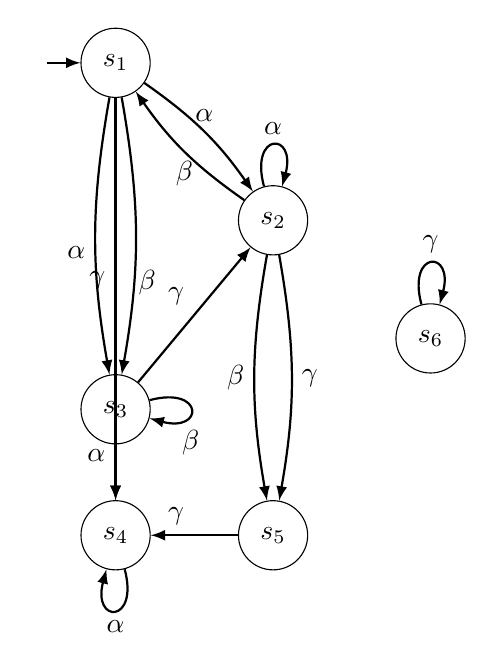
\begin{tikzpicture} [scale=2, every initial by arrow/.style={thick}]
		

		\path
		(\basex,		\basey) 		node[state,init] (s1) 	{$\state_1$} 
		(\basex+2,		\basey+0) 		node[state] (s2) 	{$\state_2$} 
		(\basex+1,		\basey-1.2) 	node[state] (s3) 	{$\state_3$} 
		(\basex,		\basey-2) 		node[state] (s4) 	{$\state_4$} 
		(\basex+2,		\basey-2) 		node[state] (s5) 	{$\state_5$}
		(\basex+3,		\basey-.75) 	node[state] (s6) 	{$\state_6$}
				
		;
		
%		
		\path [bendtrans] 	(s1) 	edge node [midway,above]				{\action} 		(s2);
		\path [bendtrans] 	(s1) 	edge node [near end,above right=-2pt]	{\actionb} 		(s3);
		\path [bendtransr] 	(s1) 	edge node [midway,below left]	{\action} 		(s3);
		\path [trans] 		(s1) 	edge node [midway,above left]	{\actionc} 		(s4);
		\path [bendtrans] 	(s2) 	edge node [midway,below]		{\actionb} 		(s1);
		\path [bendtransr] 	(s2) 	edge node [midway,left]			{\actionb} 		(s5);
		\path [bendtrans] 	(s2) 	edge node [midway,right]		{\actionc} 		(s5);
		\path [trans] 		(s3)	edge node [midway,above left]	{\actionc} 		(s2);
		\path [trans] 		(s3)	edge node [midway,above left]	{\action} 		(s4);
		\path [trans] 		(s5)	edge node [midway,above left]	{\actionc} 		(s4);
		
		\path [trans] 		(s2) 	edge [loop above] node [midway,above] {\action} 	(s2);
		\path [trans] 		(s3) 	edge [loop right] node [midway,below=4pt] {\actionb} 	(s3);
		\path [trans] 		(s4) 	edge [loop below] node [midway,below] {\action} 	(s4);
		\path [trans] 		(s6) 	edge [loop above] node [midway,above] {\actionc} 	(s6);
		
		
		%		midway, at start, near start, very near start, at end, near end, very near end
		
		
	\end{tikzpicture}
\end{document}
	\end{minipage}%
	\begin{minipage}{.5\textwidth}				
		\hspace{5mm}
		\documentclass[tikz,preview]{standalone}
%\usepackage{prelude}

%%%%%%%%%%%%%%%%%%%%%%%%%%%%%%%%%%%% PACKAGES %%%%%%%%%%%%%%%%%%%%%%%%%%%%%%%%%%%%%%%%%%

\usepackage{inputenc,fontenc}
\usepackage[a4paper,margin=3cm]{geometry}
\usepackage[english]{babel}
%\usepackage[german]{babel}
%\usepackage[fixlanguage]{babelbib}


\usepackage{bbold}
\usepackage{amsthm}
\usepackage{amsmath}
\usepackage{amssymb} % doteqdot
\usepackage[dvipsnames]{xcolor}
\usepackage{standalone}
\usepackage{tikz}[mode=buildnew]
\usepackage{cite}
\usepackage{xspace}
\usepackage{relsize}
\usepackage{mathtools} % mathclap
%\usepackage{MnSymbol}
\usepackage{hyperref}
\usepackage{url}
\usepackage{listings} % for code
\usepackage[T1]{fontenc} %<
\hypersetup{
	colorlinks,
	citecolor=black,
	filecolor=black,
	linkcolor=black,
	urlcolor=black
}
\usepackage{pgfplots}
\pgfplotsset{compat=1.18}
%\usepackage{courier} %% Sets font for listing as Courier. But also for url and texttt!
\usepackage{listings, xcolor}
\usepackage{graphicx}
\usepackage{subcaption}

\usetikzlibrary{calc}
%\usepackage{xparse} % \newDocumentCommand for multiple optional arguments
%\usepackage{titlecaps}



%%%%%%%%%%%%%%%%%%%%%%%%%%%%%%%%%%%% THEOREMSTYLES %%%%%%%%%%%%%%%%%%%%%%%%%%%%%%%%%%

\theoremstyle{definition}
\newtheorem{definition}{Definition}[section]
\newtheorem{exmp}{Beispiel}[section]
%\AfterEndEnvironment{definition}{\noindent\ignorespaces}

\theoremstyle{theorem}
\newtheorem{theorem}{Satz}[section]
\newtheorem{proposition}{Proposition}[section]
%\AfterEndEnvironment{theorem}{\noindent\ignorespaces}

\theoremstyle{korollary}
\newtheorem{korollary}{Korollar}[section]
%\AfterEndEnvironment{korollary}{\noindent\ignorespaces}


\tikzset{
	mstate/.style={draw, circle, minimum size=.94cm}, 
	gstate/.style={draw, rectangle, minimum size=.8cm},
	varstate/.style={draw,rectangle, rounded corners, minimum size=1}, 
	trans/.style={draw, ->, thick},
	bendtrans/.style={draw, ->, thick, bend left=10},
	bendtransr/.style={draw, ->, thick, bend right=10},
	init/.style={initial, initial distance=6pt, initial text=},
	every loop/.style={min distance=5pt, looseness=8},
	>=latex
}
\usetikzlibrary{automata,positioning}

%auto shift/.style={auto=right,->,
%	to path={ let \p1=(\tikztostart),\p2=(\tikztotarget),
%		\n1={atan2(\y2-\y1,\x2-\x1)},\n2={\n1+180}
%		in ($(\tikztostart.{\n1})!1mm!270:(\tikztotarget.{\n2})$) -- 
%		($(\tikztotarget.{\n2})!1mm!90:(\tikztostart.{\n1})$) \tikztonodes}},

%%%%%%%%%%%%%%%%%%%%%%%%%%%%%%%%%%% MY MACROS %%%%%%%%%%%%%%%%%%%%%%%%%%%%%%%%%%%%%%%%%
%formatting
\newcommand{\comment}[2]{{\color{#1}#2}}
\newcommand{\redcomment}[1]{{\color{red}#1}}
\newcommand{\purpcomment}[1]{{\color{pink}#1}}
\newcommand{\bluecomment}[1]{{\color{blue}#1}}
\newcommand{\mt}[1]{\ensuremath{{#1}}\xspace}
\newcommand{\mynewcommand}[2]{\newcommand{#1}{\mt{#2}}} %% currently not used becaue of ide highlighting
\newcommand{\arr}{\mt{\to}}

%model checking terms
\newcommand{\mimicrel}{\mt{\mathcal{R}}}
\newcommand{\bisimeq}{\mt{\;\!\sim\;\!}}
\newcommand{\simorder}{\mt{\;\!\preceq\;\!}}
\newcommand{\simequiv}{\mt{\;\!\simeq\;\!}} %command already defined
\newcommand{\relts}{\mt{\;\!\bullet_{_{\tiny{TS}}}\;\!}}
\newcommand{\rel}{\mt{\;\!\bullet\;\!}}

%own names
\newcommand{\nm}[1]{#1\xspace}
\newcommand{\mdpN}{\nm{MDP}}
\newcommand{\mdpsN}{\nm{MDPs}}
\newcommand{\viewN}{\nm{view}}
\newcommand{\viewNC}{\nm{View}}
\newcommand{\viewsN}{\nm{views}}
\newcommand{\viewsNC}{\nm{Views}}
\newcommand{\grpfctsubN}{\nm{detached grouping function}}
\newcommand{\grpfctsubNC}{\nm{detached grouping function}}
\newcommand{\grpfctsubNCC}{\nm{Detached Grouping Function}}
\newcommand{\grpfctN}{\nm{grouping function}}
\newcommand{\grpfctNC}{\nm{Grouping function}}
\newcommand{\grpfctNCC}{\nm{Grouping Function}}
\newcommand{\grpfctsN}{\nm{grouping functions}}
\newcommand{\grpfctsNC}{\nm{Grouping functions}}
\newcommand{\grpfctsNCC}{\nm{Grouping Functions}}
\newcommand{\stmimicN}{\nm{state-mimic}}
\newcommand{\stmimicsN}{\nm{state-mimics}}
\newcommand{\stmimickingN}{\nm{state-mimicking}}
\newcommand{\stmimickedN}{\nm{state-mimicked}}
%\newcommand{\chosenphtypeNCC}{\nm{Transition System}}
%\newcommand{\chgphNC}{\nm{Transition system}}
%\newcommand{\chgphN}{\nm{transition system}}
%\newcommand{\chgphsNCC}{\nm{Transition Systems}}
%\newcommand{\chgphsNC}{\nm{Transition systems}}
%\newcommand{\chgphsN}{\nm{transition systems}}
\newcommand{\chgphNCC}{\nm{MDP}}
\newcommand{\chgphNC}{\nm{MDP}}
\newcommand{\chgphN}{\nm{MDP}}
\newcommand{\achgphN}{\nm{an MDP}}
\newcommand{\chgphsNCC}{\nm{MDPs}}
\newcommand{\chgphsNC}{\nm{MDPs}}
\newcommand{\chgphsN}{\nm{MDPs}}
\newcommand{\parllcompN}{\nm{parallel composition}}
\newcommand{\parllcompNC}{\nm{Parallel composition}}
\newcommand{\parllcompNCC}{\nm{Parallel Composition}}
\newcommand{\parllcompsN}{\nm{parallel compositions}}
\newcommand{\parllcompsNC}{\nm{Parallel compositions}}
\newcommand{\parllcompsNCC}{\nm{Parallel Compositions}}
\newcommand{\sccN}{\nm{SCC}}
\newcommand{\sccsN}{\nm{SCCs}}
\newcommand{\bsccN}{\nm{BSCC}}
\newcommand{\bsccsN}{\nm{BSCCs}}
\newcommand{\jgrapht}{\nm{jGraphtT}}

\newcommand{\outactident}{\nm{OutActionsIdent}}

%names
\newcommand{\iffN}{\nm{if and only if}}
\newcommand{\tsN}{\nm{TS}}

%% outactions identical
\newcommand{\outactidentstrong}{\nm{strong}}
\newcommand{\outactidentweak}{\nm{weak}}

% CORE DEFINITIONS
\newcommand{\grpfct}[1][\viewppty]{\mt{F_{#1}}}
\newcommand{\grpfctsub}[1][\viewppty]{\mt{\tilde{F}_{#1}}}
%\newcommand{\grpfctimg}[1]{\mt{{\grpfct}[{#1}]}}
%\newcommand{\fctimg}[2]{\mt{{#1}[{#2}]}}
\newcommand{\eqrelview}{\mt{R}}
\newcommand{\eqclassv}[1][\state]{\mt{\eqclass{#1}{\eqrelview}}}
\newcommand{\eqclasssetv}[1][\states]{\mt{{#1}/\eqrelview}} %OLD: \bigcup_{\state \in \states} \eqclassv
\newcommand{\viewid}{\mt{\mdp}}
\newcommand{\view}[1][\viewppty]{\mt{\viewid_{#1}}}
\newcommand{\imggrp}{\mt{\arbset}}
\newcommand{\imggrpsub}{\mt{X}}
\newcommand{\viewppty}{\mt{\theta}}
\newcommand{\pll}{\mt{\;\!\pllpure\;\!}}
\newcommand{\pllrev}{\mt{\pllpure^{-1}}}
\newcommand{\pllpure}{\mt{||}}
\newcommand{\compselectset}{\mt{Z}}
\newcommand{\compselectpure}{\mt{\pllpure_\compselectset}}
\newcommand{\compselect}{\mt{\;\pllpure_\compselectset\;}}
\newcommand{\remstates}{\mt{\bigcup_{\state \in \states \setminus \states_1}\{\{\state\}\}}}
\newcommand{\nogroupstates}[1][\states_2]{\mt{\bigcup_{\state \in \states \setminus {#1}}\{\{\state\}\}}}
\newcommand{\remelem}{\mt{\bullet}}
\newcommand{\nogroupset}{\mt{\xi}}
\newcommand{\remset}{\mt{\{\remelem\}}}
\newcommand{\gfctpll}{\mt{\grpfct[\pll]}}
\newcommand{\group}{\mt{\top}}
\newcommand{\imggrpbinview}{\mt{\{\remelem, \notppty\}}}
\newcommand{\viewappset}{\mt{\tilde{\states}}}
\newcommand{\hasppty}{\mt{\top}}
\newcommand{\notppty}{\mt{\bot}}
\newcommand{\disregardelem}{\mt{\Delta}}
\newcommand{\disregardelements}{\mt{{\disregardelem_1, \dots, \disregardelem_n}}}



%\newcommand{\mdp}{def}\mdp
%\newcommand{\mdpdef}



% EXAMPLE VIEWS
\newcommand{\pptyatomicprops}{\mt{\atomicprops}}
\newcommand{\pptyinitstates}{\mt{\initstates}}
\newcommand{\pptyinactsetsize}{\mt{|\inacts(\state)|}}
\newcommand{\pptyhasoutact}{\mt{\exists\outact}}
\newcommand{\pptyminoutact}[2]{\mt{#1\leq#2}}
\newcommand{\pptymaxoutact}[2]{\mt{#2\leq#1}}
\newcommand{\pptyspanoutact}[3]{\mt{#1\leq#2\leq#3}}
\newcommand{\pptyoutactsetsize}{\mt{|\outacts(\state)|}}
\newcommand{\pptyoutactsingle}{\mt{|\outacts(\state)|_1}}
\newcommand{\pptystrongoutactident}{\mt{\outacts(\state)_=}}
\newcommand{\pptyweakoutactident}{\mt{\outacts(\state)_\approx}}
\newcommand{\pptyhasinact}{\mt{\exists\inact}}
\newcommand{\pptymininact}[2]{\mt{#1\leq#2}}
\newcommand{\pptymaxinact}[2]{\mt{#2\leq#1}}
\newcommand{\pptyspaninact}[3]{\mt{#1\leq#2\leq#3}}
\newcommand{\pptyinactsingle}{\mt{|\inacts(\state)|_1}}
\newcommand{\pptystronginactident}{\mt{\inacts(\state)_=}}
\newcommand{\pptyweakinactident}{\mt{\inacts(\state)_\approx}}
\newcommand{\pptyparamvalueseq}{\mt{\var = \varval}}
\newcommand{\pptyparamvaluesneq}{\mt{\var \neq \varval}}
\newcommand{\pptyparamdnf}{\mt{VarDNF}}
\newcommand{\pptyparamcnf}{\mt{VarCNF}}
\newcommand{\pptyparamvalueseqopt}{\mt{\var = \varval}}
\newcommand{\pptyparamvalident}{\mt{Var:\varval}}
\newcommand{\pptydistance}{\mt{\distpath}}
\newcommand{\pptydistancerev}{\mt{\distpathrev}}
\newcommand{\pptydistancebi}{\mt{\distpathbi}}
\newcommand{\pptyhascycle}{\mt{\exists\cycle}}
\newcommand{\pptyexactactcycle}{\mt{\{\cycle_{\action,n}\}}}
\newcommand{\pptycycleset}{\mt{\cup{\{\state\}_\cycle}}}
\newcommand{\pptyexactcycle}{\mt{\{\cycle_n\}}}
\newcommand{\pptyscc}{\mt{scc}}
\newcommand{\pptybscc}{\mt{bscc}}
\newcommand{\pptyprop}{\mt{\redcomment{?}}}
\newcommand{\pptyident}{id}


\newcommand{\gfctatomicprops}{\mt{\grpfct[\pptyatomicprops]}}
\newcommand{\gfctinitstates}{\mt{\grpfct[\pptyinitstates]^\hasppty}}
\newcommand{\gfcthasoutaction}{\mt{\grpfct[\pptyhasoutact]^\hasppty}}
\newcommand{\gfctminoutaction}{\mt{\grpfct[\pptyminoutact{\numoutact}{\outact}]^\hasppty}}
\newcommand{\gfctmaxoutaction}{\mt{\grpfct[\pptymaxoutact{\numoutact}{\outact}]^\hasppty}}
\newcommand{\gfctspanoutaction}{\mt{\grpfct[\pptyspanoutact{\numoutactb}{\outact}{\numoutact}]^\hasppty}}
\newcommand{\gfctoutactsetsize}{\mt{\grpfct[\pptyoutactsetsize]}}
\newcommand{\gfctoutactsingle}{\mt{\grpfct[\pptyoutactsingle]^\notppty}}
\newcommand{\gfctstrongoutactident}{\mt{\grpfct[\pptystrongoutactident]}}
\newcommand{\gfctweakoutactident}{\mt{\grpfct[\pptyweakoutactident]}}
\newcommand{\gfcthasinaction}{\mt{\grpfct[\pptyhasinact]^\hasppty}}
\newcommand{\gfctmininaction}{\mt{\grpfct[\pptymininact{\numinact}{\inact}]^\hasppty}}
\newcommand{\gfctmaxinaction}{\mt{\grpfct[\pptymaxinact{\numinact}{\inact}]^\hasppty}}
\newcommand{\gfctspaninaction}{\mt{\grpfct[\pptyspaninact{\numinactb}{\inact}{\numinact}]^\hasppty}}
\newcommand{\gfctinactsetsize}{\mt{\grpfct[\pptyinactsetsize]}}
\newcommand{\gfctinactsingle}{\mt{\grpfct[\pptyinactsingle]^\notppty}}
\newcommand{\gfctstronginactident}{\mt{\grpfct[\pptystronginactident]}}
\newcommand{\gfctweakinactident}{\mt{\grpfct[\pptyweakinactident]}}
\newcommand{\gfctparamvalueseq}{\mt{\grpfct[\pptyparamvalueseq]^\hasppty}}
\newcommand{\gfctparamvaluesneq}{\mt{\grpfct[\pptyparamvaluesneq]^\hasppty}}
\newcommand{\gfctparamdnf}{\mt{\grpfct[\pptyparamdnf]^\hasppty}}
\newcommand{\gfctparamcnf}{\mt{\grpfct[\pptyparamcnf]^\hasppty}}
\newcommand{\gfctparamvalueseqopt}{\mt{\pptyparamvalueseqopt}}
\newcommand{\gfctparamvalident}{\mt{\grpfct[\pptyparamvalident]}}
\newcommand{\gfctdistance}{\mt{\grpfct[\pptydistance]}}
\newcommand{\gfctdistancerev}{\mt{\grpfct[\pptydistancerev]}}
\newcommand{\gfctdistancebi}{\mt{\grpfct[\pptydistancebi]}}
\newcommand{\gfcthascycle}{\mt{\grpfct[\pptyhascycle]}}
\newcommand{\gfctexactcycle}{\mt{\grpfct[\pptyexactcycle]}}
\newcommand{\gfctcycleset}{\mt{\grpfct[\pptycycleset]}}
\newcommand{\gfctexactactcycle}{\mt{\grpfct[\pptyexactactcycle]}}
\newcommand{\gfctscc}{\mt{\grpfct[\pptyscc]}}
\newcommand{\gfctbscc}{\mt{\grpfct[\pptybscc]}}
\newcommand{\gfctprop}{\mt{\grpfct[\pptyprop]}}
\newcommand{\gfctident}{\mt{\grpfct[\pptyident]}}

\newcommand{\gfctsubatomicprops}{\mt{\grpfctsub[\pptyatomicprops]}}
\newcommand{\gfctsubinitstates}{\mt{\grpfctsub[\pptyinitstates]^\hasppty}}
\newcommand{\gfctsubhasoutaction}{\mt{\grpfctsub[\pptyhasoutact]^\hasppty}}
\newcommand{\gfctsubminoutaction}{\mt{\grpfctsub[\pptyminoutact{\numoutact}{\outact}]^\hasppty}}
\newcommand{\gfctsubmaxoutaction}{\mt{\grpfctsub[\pptymaxoutact{\numoutact}{\outact}]^\hasppty}}
\newcommand{\gfctsubspanoutaction}{\mt{\grpfctsub[\pptyspanoutact{\numoutactb}{\outact}{\numoutact}]^\hasppty}}
\newcommand{\gfctsuboutactsetsize}{\mt{\grpfctsub[\pptyoutactsetsize]}}
\newcommand{\gfctsuboutactsingle}{\mt{\grpfctsub[\pptyoutactsingle]^\notppty}}
\newcommand{\gfctsubstrongoutactident}{\mt{\grpfctsub[\pptystrongoutactident]^\hasppty}}
\newcommand{\gfctsubweakoutactident}{\mt{\grpfctsub[\pptyweakoutactident]^\hasppty}}
\newcommand{\gfctsubhasinaction}{\mt{\grpfctsub[\pptyhasinact]}}
\newcommand{\gfctsubmininaction}{\mt{\grpfctsub[\pptymininact{\numinact}{\inact}]}}
\newcommand{\gfctsubmaxinaction}{\mt{\grpfctsub[\pptymaxinact{\numinact}{\inact}]}}
\newcommand{\gfctsubspaninaction}{\mt{\grpfctsub[\pptyspaninact{\numinactb}{\inact}{\numinact}]}}
\newcommand{\gfctsubinactsetsize}{\mt{\grpfctsub[\pptyinactsetsize]^\hasppty}}
\newcommand{\gfctsubinactsingle}{\mt{\grpfctsub[\pptyinactsingle]^\notppty}}
\newcommand{\gfctsubstronginactident}{\mt{\grpfctsub[\pptystronginactident]}}
\newcommand{\gfctsubweakinactident}{\mt{\grpfctsub[\pptyweakinactident]}}
\newcommand{\gfctsubparamvalueseq}{\mt{\grpfctsub[\pptyparamvalueseq]^\hasppty}}
\newcommand{\gfctsubparamvaluesneq}{\mt{\grpfctsub[\pptyparamvaluesneq]^\hasppty}}
\newcommand{\gfctsubparamdnf}{\mt{\grpfctsub[\pptyparamdnf]^\hasppty}}
\newcommand{\gfctsubparamcnf}{\mt{\grpfctsub[\pptyparamcnf]^\hasppty}}
\newcommand{\gfctsubparamvalueseqopt}{\mt{\pptyparamvalueseqopt}}
\newcommand{\gfctsubparamvalident}{\mt{\grpfctsub[\pptyparamvalident]}}
\newcommand{\gfctsubdistance}{\mt{\grpfctsub[\pptydistance]}}
\newcommand{\gfctsubdistancerev}{\mt{\grpfctsub[\pptydistancerev]}}
\newcommand{\gfctsubdistancebi}{\mt{\grpfctsub[\pptydistancebi]}}
\newcommand{\gfctsubhascycle}{\mt{\grpfctsub[\pptyhascycle]^\hasppty}}
\newcommand{\gfctsubexactcycle}{\mt{\grpfctsub[\pptyexactcycle]}}
\newcommand{\gfctsubcycleset}{\mt{\grpfctsub[\pptycycleset]}}
\newcommand{\gfctsubexactactcycle}{\mt{\grpfctsub[\pptyexactactcycle]}}
\newcommand{\gfctsubscc}{\mt{\grpfctsub[\pptyscc]}}
\newcommand{\gfctsubbscc}{\mt{\grpfctsub[\pptybscc]}}
\newcommand{\gfctsubprop}{\mt{\grpfctsub[\pptyprop]}}
\newcommand{\gfctsubident}{\mt{\grpfctsub[\pptyident]}}


\newcommand{\viewatomicprops}{\mt{\view[\pptyatomicprops]}}
\newcommand{\viewinitstates}{\mt{\view[\pptyinitstates]^\hasppty}}
\newcommand{\viewhasoutaction}{\mt{\view[\pptyhasoutact]^\hasppty}}
\newcommand{\viewminoutaction}{\mt{\view[\pptyminoutact{\numoutact}{\outact}]^\hasppty}}
\newcommand{\viewmaxoutaction}{\mt{\view[\pptymaxoutact{\numoutact}{\outact}]^\hasppty}}
\newcommand{\viewspanoutaction}{\mt{\view[\pptyspanoutact{\numoutactb}{\outact}{\numoutact}]^\hasppty}}
\newcommand{\viewoutactsetsize}{\mt{\view[\pptyoutactsetsize]}}
\newcommand{\viewoutactsingle}{\mt{\view[\pptyoutactsingle]^\notppty}}
\newcommand{\viewstrongoutactident}{\mt{\view[\pptystrongoutactident]}}
\newcommand{\viewweakoutactident}{\mt{\view[\pptyweakoutactident]}}
\newcommand{\viewhasinaction}{\mt{\view[\pptyhasinact]^\hasppty}}
\newcommand{\viewmininaction}{\mt{\view[\pptymininact{\numinact}{\inact}]^\hasppty}}
\newcommand{\viewmaxinaction}{\mt{\view[\pptymaxinact{\numinact}{\inact}]^\hasppty}}
\newcommand{\viewspaninaction}{\mt{\view[\pptyspaninact{\numinactb}{\inact}{\numinact}]^\hasppty}}
\newcommand{\viewinactsetsize}{\mt{\view[\pptyinactsetsize]}}
\newcommand{\viewinactsingle}{\mt{\view[\pptyinactsingle]^\notppty}}
\newcommand{\viewstronginactident}{\mt{\view[\pptystronginactident]}}
\newcommand{\viewweakinactident}{\mt{\view[\pptyweakinactident]}}
\newcommand{\viewparamvalueseq}{\mt{\view[\pptyparamvalueseq]}}
\newcommand{\viewparamvaluesneq}{\mt{\view[\pptyparamvaluesneq]}}
\newcommand{\viewparamdnf}{\mt{\view[\pptyparamdnf]^\hasppty}}
\newcommand{\viewparamcnf}{\mt{\view[\pptyparamcnf]^\hasppty}}
\newcommand{\viewparamvalueseqopt}{\mt{\pptyparamvalueseqopt}}
\newcommand{\viewparamvalident}{\mt{\view[\pptyparamvalident]}}
\newcommand{\viewdistance}{\mt{\view[\pptydistance]}}
\newcommand{\viewdistancerev}{\mt{\view[\pptydistancerev]}}
\newcommand{\viewdistancebi}{\mt{\view[\pptydistancebi]}}
\newcommand{\viewhascycle}{\mt{\view[\pptyhascycle]}}
\newcommand{\viewexactcycle}{\mt{\view[\pptyexactcycle]}}
\newcommand{\viewcycleset}{\mt{\view[\pptycycleset]}}
\newcommand{\viewexactactcycle}{\mt{\view[\pptyexactactcycle]}}
\newcommand{\viewscc}{\mt{\view[\pptyscc]}}
\newcommand{\viewbscc}{\mt{\view[\pptybscc]}}
\newcommand{\viewprop}{\mt{\view[\pptyprop]}}
\newcommand{\viewident}{\mt{\view[\pptyident]}}

%\newcommand{\viewatomicprops}{\mt{\view[\atomicprops]}}
%\newcommand{\viewinitstates}{\mt{\view[\initstates]}}
%\newcommand{\viewhasoutaction}{\mt{\view[\pptyhasoutact]}}
%\newcommand{\viewminoutaction}{\mt{\view[\pptyminoutact{\numoutact}{\outact}]}}
%\newcommand{\viewmaxoutaction}{\mt{\view[\pptymaxoutact{\numoutact}{\outact}]}}
%\newcommand{\viewspanoutaction}{\mt{\view[\pptyspanoutact{\numoutactb}{\outact}{\numoutact}]}}
%\newcommand{\viewoutactsetsize}{\mt{\view[\pptyoutactsetsize]}}
%\newcommand{\viewoutactsingle}{\mt{\view[\pptyoutactsingle]}}
%\newcommand{\viewstrongoutactident}{\mt{\view[\outacts(\state)_=]}}
%\newcommand{\viewweakoutactident}{\mt{\view[\outacts(\state)_\approx]}}
%\newcommand{\viewhasinaction}{\mt{\view[\pptyhasinact]}}
%\newcommand{\viewmininaction}{\mt{\view[\pptymininact{\numinact}{\inact}]}}
%\newcommand{\viewmaxinaction}{\mt{\view[\pptymaxinact{\numinact}{\inact}]}}
%\newcommand{\viewspaninaction}{\mt{\view[\pptyspaninact{\numinactb}{\inact}{\numinact}]}}
%\newcommand{\viewinactsetsize}{\mt{\view[\pptyinactsetsize]}}
%\newcommand{\viewinactsingle}{\mt{\view[\pptyinactsingle]}}
%\newcommand{\viewstronginactident}{\mt{\view[\inacts(\state)_=]}}
%\newcommand{\viewweakinactident}{\mt{\view[\inacts(\state)_\approx]}}
%\newcommand{\viewparamvalueseq}{\mt{\view[\var = \varval]}}
%\newcommand{\viewparamvaluesneq}{\mt{\view[\var \neq \varval]}}
%\newcommand{\viewparamdnf}{\mt{\view[VarDNF]}}
%\newcommand{\viewparamcnf}{\mt{\view[VarCNF]}}
%\newcommand{\viewparamvalident}{\mt{\view[\pptyparamvalident]}}
%\newcommand{\viewdistance}{\mt{\view[\pptydistance]}}
%\newcommand{\viewhascycle}{\mt{\view[\exists\cycle]}}
%\newcommand{\viewexactcycle}{\mt{\view[\pptyexactcycle]}}
%\newcommand{\viewcycleset}{\mt{\view[\pptycycleset]}}
%\newcommand{\viewexactactcycle}{\mt{\view[\pptyexactactcycle]}}
%\newcommand{\viewscc}{\mt{\view[scc]}}
%\newcommand{\viewbscc}{\mt{\view[bscc]}}

%actions
\newcommand{\numoutact}{\mt{n}}
\newcommand{\numoutactb}{\mt{m}}
\newcommand{\numinact}{\mt{n}}
\newcommand{\numinactb}{\mt{m}}

\newcommand{\predmaxoutact}[1][\numoutact]{\mt{Q_{\outact\leq#1}(\state,\state_1, \dots, \state_{#1+1})}}
\newcommand{\predminoutact}[1][\numoutact]{\mt{Q_{#1\leq\outact}(\state,\state_1, \dots, \state_{#1})}}
\newcommand{\formoutact}[1][\state]{\mt{C_{#1,\outact}}}
\newcommand{\predmaxinact}[1][\numinact]{\mt{Q_{\inact\leq#1}(\state,\state_1, \dots, \state_{#1+1})}}
\newcommand{\predmininact}[1][\numinact]{\mt{Q_{#1\leq\inact}(\state,\state_1, \dots, \state_{#1})}}

\newcommand{\outact}[1][\action]{\mt{\overrightarrow{#1}}}
\newcommand{\outacts}{\mt{\overrightarrow{\actions}}}
\newcommand{\inact}{\mt{\overleftarrow{\action}}}
\newcommand{\inacts}[1][\action]{\mt{\overleftarrow{#1}}}

%%Parameters
\newcommand{\vars}[1][\mdp]{\mt{V\!ar_{#1}}}
\newcommand{\var}{\mt{x}}
\newcommand{\varstate}[1][]{\mt{\var_{\state#1}}}
\newcommand{\varval}{\mt{a}}
\newcommand{\vareval}[1][\mdp]{\mt{V\!arEval_{#1}}}
\newcommand{\varevalimg}[1][\mdp]{\mt{\vareval[#1][\states,\vars]}}
\newcommand{\varevalimgset}{\mt{\arbset}}
\newcommand{\someparam}{\mt{\tilde{x}}}
\newcommand{\eqorneq}{\mt{\;\doteqdot\;}}
\newcommand{\varstyle}[2]{\mt{\langle#1,#2\rangle}}




%\makeatletter
%\newcommand{\overleftrightsmallarrow}{\mathpalette{\overarrowsmall@\leftrightarrowfill@}}
%\newcommand{\overrightsmallarrow}{\mathpalette{\overarrowsmall@\rightarrowfill@}}
%\newcommand{\overleftsmallarrow}{\mathpalette{\overarrowsmall@\leftarrowfill@}}
%\newcommand{\overarrowsmall@}[3]{%
%	\vbox{%
%		\ialign{%
%			##\crcr
%			#1{\smaller@style{#2}}\crcr
%			\noalign{\nointerlineskip}%
%			$\m@th\hfil#2#3\hfil$\crcr
%		}%
%	}%
%}
%\def\smaller@style#1{%
%	\ifx#1\displaystyle\scriptstyle\else
%	\ifx#1\textstyle\scriptstyle\else
%	\scriptscriptstyle
%	\fi
%	\fi
%}
%\makeatother
%\newcommand{\te}[1]{\overleftrightsmallarrow{#1}}

% Distance
\newcommand{\fctdist}{\mt{distance}}
\newcommand{\fctdistdefault}{\mt{\fctdist(\chgph, \smstates, \grandist)}}
\newcommand{\distval}{\mt{d}}
\newcommand{\grandist}{\mt{n}}
\let\path\oldpath
\newcommand{\path}{\mt{P}}
\newcommand{\pathbi}{\mt{\bar{\path}}}
\newcommand{\pathsecfull}{\mt{(\state_0, \action_0, \state_1, \action_1, \dots, \action_{n}, \state_{n+1})}}
\newcommand{\lenpath}{\mt{len}}
\newcommand{\pfirst}{\mt{first}}
\newcommand{\plast}{\mt{last}}
\newcommand{\pathset}{\mt{\path_\chgph}}
\newcommand{\pathbiset}{\mt{\pathbi_\chgph}}
\newcommand{\distpath}{\mt{\overrightarrow{dist}}}
\newcommand{\distpathrev}{\mt{\overleftarrow{dist}}}
\newcommand{\distpathbi}{\mt{\overline{dist}}}
%Cycles
\newcommand{\cyclesecfull}{\mt{(\state_0, \action_0, \state_1, \action_1, \dots, \action_{n-1}, \state_0)}}
\newcommand{\fctfindcycles}{\mt{findCycles}}
\newcommand{\cycle}{\mt{C}}
\newcommand{\cycleset}{\mt{\cycle_{\mdp, n}}}
\newcommand{\lencycle}{\mt{len}}
% strongly connected components
\newcommand{\scc}{\mt{T}}
\newcommand{\setscc}{\mt{SCC_{\chgph,n}}}
\newcommand{\setbscc}{\mt{BSCC_{\chgph,n}}}

% properties
\newcommand{\propfct}{\mt{f}}

% all Systems
\newcommand{\chgph}{\mt{\mdp}}
\newcommand{\chgphtuple}{\mt{\mdptuple}}
\newcommand{\chgphtupledist}{\mt{\mdptupledist}}

\newcommand{\states}{\mt{S}}
\newcommand{\actions}{\mt{Act}}
\newcommand{\atomicprops}{\mt{AP}}
\newcommand{\labelingfct}{\mt{L}}
\newcommand{\init}{\mt{\initdistrib}} % use MDP % refers to the underlying set
\newcommand{\trans}{\mt{\probtfunc}} % use MDP % refers to the underlying set
\newcommand{\smstates}{\mt{\tilde{\states}}}


\newcommand{\state}{\mt{s}}
\newcommand{\action}{\mt{\alpha}}
\newcommand{\actionb}{\mt{\beta}}
\newcommand{\actionc}{\mt{\gamma}}
\newcommand{\smstate}{\mt{\tilde{\state}}}



% transition sysstems
\newcommand{\ts}{\mt{TS}}
\newcommand{\transitionrel}{\mt{\longrightarrow}}
\newcommand{\initstates}{\mt{I}}
\newcommand{\transitionsystem}{\mt
	{(\states, \actions, \transitionrel, \initstates, \atomicprops, \labelingfct)}
}
\newcommand{\tstupledist}{\mt{(\states', \actions',\transitionrel', \initstates', \labelingfct')}}


%Markov chains and MDP
\newcommand{\mdp}{\mt{\autm}}
\newcommand{\mdptuple}{\mt{(\states, \actions, \probtfunc, \initdistrib, \atomicprops, \labelingfct)}}
\newcommand{\mdptupledist}{\mt{(\states', \actions', \probtfunc', \initdistrib', \atomicprops', \labelingfct')}}
\newcommand{\autm}{\mt{\mathcal{M}}}
\newcommand{\probtfunc}{\mt{\textbf{P}}}
\newcommand{\initdistrib}{\mt{\iota_{init}}}


%maths
\newcommand{\powerset}[1]{\mt{\mathcal{P}(#1)}}
\newcommand{\eqclass}[2]{\mt{[#1]_{#2}}}%{\mt{#1 / #2}}
\newcommand{\impr}{\mt{\hspace{3mm}\Rightarrow\hspace{2mm}}}
\newcommand{\impl}{\mt{\hspace{3mm}\Leftarrow\hspace{2mm}}}
\newcommand{\natnums}{\mt{\mathbb{N}}} 
\newcommand{\realnums}{\mt{\mathbb{R}}}
\newcommand{\intmodn}[1][n]{\mt{\mathbb{Z}_{#1}}}
\newcommand{\arbset}{\mt{M}}
\newcommand{\bigsum}[2][]{\mt{\mathlarger{\sum}_{#2}^{#1}}}
\newcommand{\bbigsum}[2][]{\mt{\mathlarger{\mathlarger{\sum}}_{#2}^{#1}}}
\newcommand{\invimage}[2]{#1^{\mt{-1}(#2)}}
\newcommand{\img}{\mt{Img}}
\newcommand{\cond}{\mt{\,|\,}}

%tickz
%% \definecolor{darkred}{RGB}{196, 42, 42}

%implementation
\newcommand{\pmcvis}{\nm{PMC-Vis}}





\begin{document}
	\newcommand{\basex}{0}
	\newcommand{\basey}{0}
	\newcommand{\createstate}[3]{\node[draw, circle, minimum size=1cm] (#1) at (#2) {#3}}
	
	
	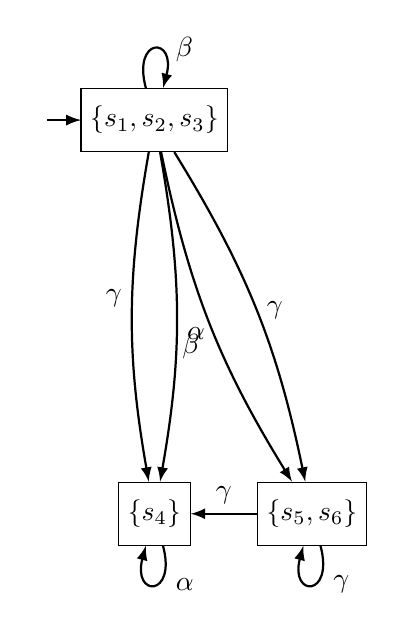
\begin{tikzpicture} [scale=2, every initial by arrow/.style={thick}]
		
		
%		\path
%		(\basex+1,		\basey) 		node[gstate,init, initial left] (s123) 	{$\state_1, \state_2,\state_3$} 
%		(\basex,		\basey-1.5) 	node[gstate] (s4) 	{$\state_4$} 
%		(\basex+2,		\basey-1.5)		node[gstate] (s56) 	{$\state_5,\state_6$} 
%		
%		(s123)++(0.25,0)		node[minimum size=0.8cm] (s123loop) 	{} 
%		(s56)++(0.1,0)		node[minimum size=0.8cm] (s56loop) 	{} 
%		
%		;
		\path
		(\basex+1,		\basey) 		node[gstate,init, initial left] (s123) 	{$\{\state_1, \state_2,\state_3\}$} 
		(\basex,		\basey-1.5) 	node[gstate] (s4) 	{$\{\state_4\}$} 
		(\basex+2,		\basey-1.5)		node[gstate] (s56) 	{$\{\state_5,\state_6\}$} 
		
		(s123)++(0.25,0)		node[minimum size=0.8cm] (s123loop) 	{} 
		(s56)++(0.1,0)		node[minimum size=0.8cm] (s56loop) 	{} 
		
		;
		
		\path [bendtransr] 		(s123) 	edge node [midway,above left]		{\actionc} 		(s4);
		\path [bendtrans] 		(s123) 	edge node [midway,below right]		{\action} 		(s4);		
		\path [bendtransr](s123) 	edge node [midway,below left]			{\actionb} 		(s56);
		\path [bendtrans] (s123) 	edge node [midway,right]		{\actionc} 		(s56);
		
		
		\path [trans] 	(s56) 	edge node [midway,above]	{\actionc} 		(s4);
		\path [trans]	(s123) edge [loop above] node [midway, right=4pt] {\actionb}	(s123);	
%		\path [trans] 		(s123loop) 	edge [loop, in=10, out=60,looseness=6, shorten >= -1pt] node [midway,right] {\actionb} 	(s123loop);
		\path [trans] 		(s4) 	edge [loop below] node [midway,right=4pt] {\action} 	(s4);
		\path [trans]		(s56) 	edge [loop below] node [midway,right=4pt] {\actionc} (s56);
%		\path [trans] 		(s56loop) 	edge [loop right] node [midway,above] {\actionc} 	(s56loop);
		
		
	\end{tikzpicture}
\end{document}
	\end{minipage}	
	\caption{Simplified representations of \mdp (left) and the \viewN \viewweakoutactident on it (right)}	
	\label{fig:outActIdentWeakAfter}  	
\end{figure}


\begin{definition}
	Let $\chgph = \chgphtuple$ be \achgphN and $\action \in \actions$. The \viewN \viewweakoutactident is defined by its \grpfctN $\gfctweakoutactident : \states \to \imggrp$ with
	\[
	\state \mapsto \{\action \in \actions \mid \exists \state' \in \states : (\state, \action, \state') \in \trans\} 	
	\]
	and $\imggrp := \actions \cup \remset$.
\end{definition}
\redcomment{condition of image-set written in inconsistent style to strong identity. Swap strong and weak (order)?}

\redcomment{The grouping function maps to the set of outgoing actions of a state and thereby discards information about the number of times an actions is outgoing. If an action is not outgoing from a state it is not contained in the set.}

For $\state_1, \state_2 \in \states$ it is $\gfctweakoutactident(\state_1) = \gfctweakoutactident(\state_2)$ \iffN they are mapped to the same set of actions. Hence the equivalence classes of \eqrelview are
\[
	\eqclassv[\smstate] = \{ \state \in \states \mid \gfctweakoutactident(\state) = \gfctweakoutactident(\smstate) =: \{\action_1, \dots, \action_l\}, l \in \natnums\}.
\]
According to Definition \ref{def:view} the set $\states' := \bigcup_{\state \in \states} \eqclassv$ is the set of states of \viewweakoutactident.

Apart from the option of directly considering one or a set of outgoing actions with possible quantities it is also possible to only consider the quantity of outgoing actions without regarding the any specific action.

\begin{definition}
	Let $\chgph = \chgphtuple$ be \achgphN and $\action \in \actions$. The \viewN \viewoutactsetsize is defined by its \grpfctN $\gfctoutactsetsize : \states \to \imggrp$ with
	\[
	\state \mapsto |\{\action \in \actions \mid \exists \state' \in \states : (\state, \action, \state') \in \trans\}|
	\]
	and $\imggrp := \natnums \cup \remset$.
\end{definition}

\begin{figure}[h]
	\begin{minipage}{.5\textwidth}
		\hspace{5mm}
		\documentclass[tikz,preview]{standalone}
%\usepackage{prelude}

%%%%%%%%%%%%%%%%%%%%%%%%%%%%%%%%%%%% PACKAGES %%%%%%%%%%%%%%%%%%%%%%%%%%%%%%%%%%%%%%%%%%

\usepackage{inputenc,fontenc}
\usepackage[a4paper,margin=3cm]{geometry}
\usepackage[english]{babel}
%\usepackage[german]{babel}
%\usepackage[fixlanguage]{babelbib}


\usepackage{bbold}
\usepackage{amsthm}
\usepackage{amsmath}
\usepackage{amssymb} % doteqdot
\usepackage[dvipsnames]{xcolor}
\usepackage{standalone}
\usepackage{tikz}[mode=buildnew]
\usepackage{cite}
\usepackage{xspace}
\usepackage{relsize}
\usepackage{mathtools} % mathclap
%\usepackage{MnSymbol}
\usepackage{hyperref}
\usepackage{url}
\usepackage{listings} % for code
\usepackage[T1]{fontenc} %<
\hypersetup{
	colorlinks,
	citecolor=black,
	filecolor=black,
	linkcolor=black,
	urlcolor=black
}
\usepackage{pgfplots}
\pgfplotsset{compat=1.18}
%\usepackage{courier} %% Sets font for listing as Courier. But also for url and texttt!
\usepackage{listings, xcolor}
\usepackage{graphicx}
\usepackage{subcaption}

\usetikzlibrary{calc}
%\usepackage{xparse} % \newDocumentCommand for multiple optional arguments
%\usepackage{titlecaps}



%%%%%%%%%%%%%%%%%%%%%%%%%%%%%%%%%%%% THEOREMSTYLES %%%%%%%%%%%%%%%%%%%%%%%%%%%%%%%%%%

\theoremstyle{definition}
\newtheorem{definition}{Definition}[section]
\newtheorem{exmp}{Beispiel}[section]
%\AfterEndEnvironment{definition}{\noindent\ignorespaces}

\theoremstyle{theorem}
\newtheorem{theorem}{Satz}[section]
\newtheorem{proposition}{Proposition}[section]
%\AfterEndEnvironment{theorem}{\noindent\ignorespaces}

\theoremstyle{korollary}
\newtheorem{korollary}{Korollar}[section]
%\AfterEndEnvironment{korollary}{\noindent\ignorespaces}


\tikzset{
	mstate/.style={draw, circle, minimum size=.94cm}, 
	gstate/.style={draw, rectangle, minimum size=.8cm},
	varstate/.style={draw,rectangle, rounded corners, minimum size=1}, 
	trans/.style={draw, ->, thick},
	bendtrans/.style={draw, ->, thick, bend left=10},
	bendtransr/.style={draw, ->, thick, bend right=10},
	init/.style={initial, initial distance=6pt, initial text=},
	every loop/.style={min distance=5pt, looseness=8},
	>=latex
}
\usetikzlibrary{automata,positioning}

%auto shift/.style={auto=right,->,
%	to path={ let \p1=(\tikztostart),\p2=(\tikztotarget),
%		\n1={atan2(\y2-\y1,\x2-\x1)},\n2={\n1+180}
%		in ($(\tikztostart.{\n1})!1mm!270:(\tikztotarget.{\n2})$) -- 
%		($(\tikztotarget.{\n2})!1mm!90:(\tikztostart.{\n1})$) \tikztonodes}},

%%%%%%%%%%%%%%%%%%%%%%%%%%%%%%%%%%% MY MACROS %%%%%%%%%%%%%%%%%%%%%%%%%%%%%%%%%%%%%%%%%
%formatting
\newcommand{\comment}[2]{{\color{#1}#2}}
\newcommand{\redcomment}[1]{{\color{red}#1}}
\newcommand{\purpcomment}[1]{{\color{pink}#1}}
\newcommand{\bluecomment}[1]{{\color{blue}#1}}
\newcommand{\mt}[1]{\ensuremath{{#1}}\xspace}
\newcommand{\mynewcommand}[2]{\newcommand{#1}{\mt{#2}}} %% currently not used becaue of ide highlighting
\newcommand{\arr}{\mt{\to}}

%model checking terms
\newcommand{\mimicrel}{\mt{\mathcal{R}}}
\newcommand{\bisimeq}{\mt{\;\!\sim\;\!}}
\newcommand{\simorder}{\mt{\;\!\preceq\;\!}}
\newcommand{\simequiv}{\mt{\;\!\simeq\;\!}} %command already defined
\newcommand{\relts}{\mt{\;\!\bullet_{_{\tiny{TS}}}\;\!}}
\newcommand{\rel}{\mt{\;\!\bullet\;\!}}

%own names
\newcommand{\nm}[1]{#1\xspace}
\newcommand{\mdpN}{\nm{MDP}}
\newcommand{\mdpsN}{\nm{MDPs}}
\newcommand{\viewN}{\nm{view}}
\newcommand{\viewNC}{\nm{View}}
\newcommand{\viewsN}{\nm{views}}
\newcommand{\viewsNC}{\nm{Views}}
\newcommand{\grpfctsubN}{\nm{detached grouping function}}
\newcommand{\grpfctsubNC}{\nm{detached grouping function}}
\newcommand{\grpfctsubNCC}{\nm{Detached Grouping Function}}
\newcommand{\grpfctN}{\nm{grouping function}}
\newcommand{\grpfctNC}{\nm{Grouping function}}
\newcommand{\grpfctNCC}{\nm{Grouping Function}}
\newcommand{\grpfctsN}{\nm{grouping functions}}
\newcommand{\grpfctsNC}{\nm{Grouping functions}}
\newcommand{\grpfctsNCC}{\nm{Grouping Functions}}
\newcommand{\stmimicN}{\nm{state-mimic}}
\newcommand{\stmimicsN}{\nm{state-mimics}}
\newcommand{\stmimickingN}{\nm{state-mimicking}}
\newcommand{\stmimickedN}{\nm{state-mimicked}}
%\newcommand{\chosenphtypeNCC}{\nm{Transition System}}
%\newcommand{\chgphNC}{\nm{Transition system}}
%\newcommand{\chgphN}{\nm{transition system}}
%\newcommand{\chgphsNCC}{\nm{Transition Systems}}
%\newcommand{\chgphsNC}{\nm{Transition systems}}
%\newcommand{\chgphsN}{\nm{transition systems}}
\newcommand{\chgphNCC}{\nm{MDP}}
\newcommand{\chgphNC}{\nm{MDP}}
\newcommand{\chgphN}{\nm{MDP}}
\newcommand{\achgphN}{\nm{an MDP}}
\newcommand{\chgphsNCC}{\nm{MDPs}}
\newcommand{\chgphsNC}{\nm{MDPs}}
\newcommand{\chgphsN}{\nm{MDPs}}
\newcommand{\parllcompN}{\nm{parallel composition}}
\newcommand{\parllcompNC}{\nm{Parallel composition}}
\newcommand{\parllcompNCC}{\nm{Parallel Composition}}
\newcommand{\parllcompsN}{\nm{parallel compositions}}
\newcommand{\parllcompsNC}{\nm{Parallel compositions}}
\newcommand{\parllcompsNCC}{\nm{Parallel Compositions}}
\newcommand{\sccN}{\nm{SCC}}
\newcommand{\sccsN}{\nm{SCCs}}
\newcommand{\bsccN}{\nm{BSCC}}
\newcommand{\bsccsN}{\nm{BSCCs}}
\newcommand{\jgrapht}{\nm{jGraphtT}}

\newcommand{\outactident}{\nm{OutActionsIdent}}

%names
\newcommand{\iffN}{\nm{if and only if}}
\newcommand{\tsN}{\nm{TS}}

%% outactions identical
\newcommand{\outactidentstrong}{\nm{strong}}
\newcommand{\outactidentweak}{\nm{weak}}

% CORE DEFINITIONS
\newcommand{\grpfct}[1][\viewppty]{\mt{F_{#1}}}
\newcommand{\grpfctsub}[1][\viewppty]{\mt{\tilde{F}_{#1}}}
%\newcommand{\grpfctimg}[1]{\mt{{\grpfct}[{#1}]}}
%\newcommand{\fctimg}[2]{\mt{{#1}[{#2}]}}
\newcommand{\eqrelview}{\mt{R}}
\newcommand{\eqclassv}[1][\state]{\mt{\eqclass{#1}{\eqrelview}}}
\newcommand{\eqclasssetv}[1][\states]{\mt{{#1}/\eqrelview}} %OLD: \bigcup_{\state \in \states} \eqclassv
\newcommand{\viewid}{\mt{\mdp}}
\newcommand{\view}[1][\viewppty]{\mt{\viewid_{#1}}}
\newcommand{\imggrp}{\mt{\arbset}}
\newcommand{\imggrpsub}{\mt{X}}
\newcommand{\viewppty}{\mt{\theta}}
\newcommand{\pll}{\mt{\;\!\pllpure\;\!}}
\newcommand{\pllrev}{\mt{\pllpure^{-1}}}
\newcommand{\pllpure}{\mt{||}}
\newcommand{\compselectset}{\mt{Z}}
\newcommand{\compselectpure}{\mt{\pllpure_\compselectset}}
\newcommand{\compselect}{\mt{\;\pllpure_\compselectset\;}}
\newcommand{\remstates}{\mt{\bigcup_{\state \in \states \setminus \states_1}\{\{\state\}\}}}
\newcommand{\nogroupstates}[1][\states_2]{\mt{\bigcup_{\state \in \states \setminus {#1}}\{\{\state\}\}}}
\newcommand{\remelem}{\mt{\bullet}}
\newcommand{\nogroupset}{\mt{\xi}}
\newcommand{\remset}{\mt{\{\remelem\}}}
\newcommand{\gfctpll}{\mt{\grpfct[\pll]}}
\newcommand{\group}{\mt{\top}}
\newcommand{\imggrpbinview}{\mt{\{\remelem, \notppty\}}}
\newcommand{\viewappset}{\mt{\tilde{\states}}}
\newcommand{\hasppty}{\mt{\top}}
\newcommand{\notppty}{\mt{\bot}}
\newcommand{\disregardelem}{\mt{\Delta}}
\newcommand{\disregardelements}{\mt{{\disregardelem_1, \dots, \disregardelem_n}}}



%\newcommand{\mdp}{def}\mdp
%\newcommand{\mdpdef}



% EXAMPLE VIEWS
\newcommand{\pptyatomicprops}{\mt{\atomicprops}}
\newcommand{\pptyinitstates}{\mt{\initstates}}
\newcommand{\pptyinactsetsize}{\mt{|\inacts(\state)|}}
\newcommand{\pptyhasoutact}{\mt{\exists\outact}}
\newcommand{\pptyminoutact}[2]{\mt{#1\leq#2}}
\newcommand{\pptymaxoutact}[2]{\mt{#2\leq#1}}
\newcommand{\pptyspanoutact}[3]{\mt{#1\leq#2\leq#3}}
\newcommand{\pptyoutactsetsize}{\mt{|\outacts(\state)|}}
\newcommand{\pptyoutactsingle}{\mt{|\outacts(\state)|_1}}
\newcommand{\pptystrongoutactident}{\mt{\outacts(\state)_=}}
\newcommand{\pptyweakoutactident}{\mt{\outacts(\state)_\approx}}
\newcommand{\pptyhasinact}{\mt{\exists\inact}}
\newcommand{\pptymininact}[2]{\mt{#1\leq#2}}
\newcommand{\pptymaxinact}[2]{\mt{#2\leq#1}}
\newcommand{\pptyspaninact}[3]{\mt{#1\leq#2\leq#3}}
\newcommand{\pptyinactsingle}{\mt{|\inacts(\state)|_1}}
\newcommand{\pptystronginactident}{\mt{\inacts(\state)_=}}
\newcommand{\pptyweakinactident}{\mt{\inacts(\state)_\approx}}
\newcommand{\pptyparamvalueseq}{\mt{\var = \varval}}
\newcommand{\pptyparamvaluesneq}{\mt{\var \neq \varval}}
\newcommand{\pptyparamdnf}{\mt{VarDNF}}
\newcommand{\pptyparamcnf}{\mt{VarCNF}}
\newcommand{\pptyparamvalueseqopt}{\mt{\var = \varval}}
\newcommand{\pptyparamvalident}{\mt{Var:\varval}}
\newcommand{\pptydistance}{\mt{\distpath}}
\newcommand{\pptydistancerev}{\mt{\distpathrev}}
\newcommand{\pptydistancebi}{\mt{\distpathbi}}
\newcommand{\pptyhascycle}{\mt{\exists\cycle}}
\newcommand{\pptyexactactcycle}{\mt{\{\cycle_{\action,n}\}}}
\newcommand{\pptycycleset}{\mt{\cup{\{\state\}_\cycle}}}
\newcommand{\pptyexactcycle}{\mt{\{\cycle_n\}}}
\newcommand{\pptyscc}{\mt{scc}}
\newcommand{\pptybscc}{\mt{bscc}}
\newcommand{\pptyprop}{\mt{\redcomment{?}}}
\newcommand{\pptyident}{id}


\newcommand{\gfctatomicprops}{\mt{\grpfct[\pptyatomicprops]}}
\newcommand{\gfctinitstates}{\mt{\grpfct[\pptyinitstates]^\hasppty}}
\newcommand{\gfcthasoutaction}{\mt{\grpfct[\pptyhasoutact]^\hasppty}}
\newcommand{\gfctminoutaction}{\mt{\grpfct[\pptyminoutact{\numoutact}{\outact}]^\hasppty}}
\newcommand{\gfctmaxoutaction}{\mt{\grpfct[\pptymaxoutact{\numoutact}{\outact}]^\hasppty}}
\newcommand{\gfctspanoutaction}{\mt{\grpfct[\pptyspanoutact{\numoutactb}{\outact}{\numoutact}]^\hasppty}}
\newcommand{\gfctoutactsetsize}{\mt{\grpfct[\pptyoutactsetsize]}}
\newcommand{\gfctoutactsingle}{\mt{\grpfct[\pptyoutactsingle]^\notppty}}
\newcommand{\gfctstrongoutactident}{\mt{\grpfct[\pptystrongoutactident]}}
\newcommand{\gfctweakoutactident}{\mt{\grpfct[\pptyweakoutactident]}}
\newcommand{\gfcthasinaction}{\mt{\grpfct[\pptyhasinact]^\hasppty}}
\newcommand{\gfctmininaction}{\mt{\grpfct[\pptymininact{\numinact}{\inact}]^\hasppty}}
\newcommand{\gfctmaxinaction}{\mt{\grpfct[\pptymaxinact{\numinact}{\inact}]^\hasppty}}
\newcommand{\gfctspaninaction}{\mt{\grpfct[\pptyspaninact{\numinactb}{\inact}{\numinact}]^\hasppty}}
\newcommand{\gfctinactsetsize}{\mt{\grpfct[\pptyinactsetsize]}}
\newcommand{\gfctinactsingle}{\mt{\grpfct[\pptyinactsingle]^\notppty}}
\newcommand{\gfctstronginactident}{\mt{\grpfct[\pptystronginactident]}}
\newcommand{\gfctweakinactident}{\mt{\grpfct[\pptyweakinactident]}}
\newcommand{\gfctparamvalueseq}{\mt{\grpfct[\pptyparamvalueseq]^\hasppty}}
\newcommand{\gfctparamvaluesneq}{\mt{\grpfct[\pptyparamvaluesneq]^\hasppty}}
\newcommand{\gfctparamdnf}{\mt{\grpfct[\pptyparamdnf]^\hasppty}}
\newcommand{\gfctparamcnf}{\mt{\grpfct[\pptyparamcnf]^\hasppty}}
\newcommand{\gfctparamvalueseqopt}{\mt{\pptyparamvalueseqopt}}
\newcommand{\gfctparamvalident}{\mt{\grpfct[\pptyparamvalident]}}
\newcommand{\gfctdistance}{\mt{\grpfct[\pptydistance]}}
\newcommand{\gfctdistancerev}{\mt{\grpfct[\pptydistancerev]}}
\newcommand{\gfctdistancebi}{\mt{\grpfct[\pptydistancebi]}}
\newcommand{\gfcthascycle}{\mt{\grpfct[\pptyhascycle]}}
\newcommand{\gfctexactcycle}{\mt{\grpfct[\pptyexactcycle]}}
\newcommand{\gfctcycleset}{\mt{\grpfct[\pptycycleset]}}
\newcommand{\gfctexactactcycle}{\mt{\grpfct[\pptyexactactcycle]}}
\newcommand{\gfctscc}{\mt{\grpfct[\pptyscc]}}
\newcommand{\gfctbscc}{\mt{\grpfct[\pptybscc]}}
\newcommand{\gfctprop}{\mt{\grpfct[\pptyprop]}}
\newcommand{\gfctident}{\mt{\grpfct[\pptyident]}}

\newcommand{\gfctsubatomicprops}{\mt{\grpfctsub[\pptyatomicprops]}}
\newcommand{\gfctsubinitstates}{\mt{\grpfctsub[\pptyinitstates]^\hasppty}}
\newcommand{\gfctsubhasoutaction}{\mt{\grpfctsub[\pptyhasoutact]^\hasppty}}
\newcommand{\gfctsubminoutaction}{\mt{\grpfctsub[\pptyminoutact{\numoutact}{\outact}]^\hasppty}}
\newcommand{\gfctsubmaxoutaction}{\mt{\grpfctsub[\pptymaxoutact{\numoutact}{\outact}]^\hasppty}}
\newcommand{\gfctsubspanoutaction}{\mt{\grpfctsub[\pptyspanoutact{\numoutactb}{\outact}{\numoutact}]^\hasppty}}
\newcommand{\gfctsuboutactsetsize}{\mt{\grpfctsub[\pptyoutactsetsize]}}
\newcommand{\gfctsuboutactsingle}{\mt{\grpfctsub[\pptyoutactsingle]^\notppty}}
\newcommand{\gfctsubstrongoutactident}{\mt{\grpfctsub[\pptystrongoutactident]^\hasppty}}
\newcommand{\gfctsubweakoutactident}{\mt{\grpfctsub[\pptyweakoutactident]^\hasppty}}
\newcommand{\gfctsubhasinaction}{\mt{\grpfctsub[\pptyhasinact]}}
\newcommand{\gfctsubmininaction}{\mt{\grpfctsub[\pptymininact{\numinact}{\inact}]}}
\newcommand{\gfctsubmaxinaction}{\mt{\grpfctsub[\pptymaxinact{\numinact}{\inact}]}}
\newcommand{\gfctsubspaninaction}{\mt{\grpfctsub[\pptyspaninact{\numinactb}{\inact}{\numinact}]}}
\newcommand{\gfctsubinactsetsize}{\mt{\grpfctsub[\pptyinactsetsize]^\hasppty}}
\newcommand{\gfctsubinactsingle}{\mt{\grpfctsub[\pptyinactsingle]^\notppty}}
\newcommand{\gfctsubstronginactident}{\mt{\grpfctsub[\pptystronginactident]}}
\newcommand{\gfctsubweakinactident}{\mt{\grpfctsub[\pptyweakinactident]}}
\newcommand{\gfctsubparamvalueseq}{\mt{\grpfctsub[\pptyparamvalueseq]^\hasppty}}
\newcommand{\gfctsubparamvaluesneq}{\mt{\grpfctsub[\pptyparamvaluesneq]^\hasppty}}
\newcommand{\gfctsubparamdnf}{\mt{\grpfctsub[\pptyparamdnf]^\hasppty}}
\newcommand{\gfctsubparamcnf}{\mt{\grpfctsub[\pptyparamcnf]^\hasppty}}
\newcommand{\gfctsubparamvalueseqopt}{\mt{\pptyparamvalueseqopt}}
\newcommand{\gfctsubparamvalident}{\mt{\grpfctsub[\pptyparamvalident]}}
\newcommand{\gfctsubdistance}{\mt{\grpfctsub[\pptydistance]}}
\newcommand{\gfctsubdistancerev}{\mt{\grpfctsub[\pptydistancerev]}}
\newcommand{\gfctsubdistancebi}{\mt{\grpfctsub[\pptydistancebi]}}
\newcommand{\gfctsubhascycle}{\mt{\grpfctsub[\pptyhascycle]^\hasppty}}
\newcommand{\gfctsubexactcycle}{\mt{\grpfctsub[\pptyexactcycle]}}
\newcommand{\gfctsubcycleset}{\mt{\grpfctsub[\pptycycleset]}}
\newcommand{\gfctsubexactactcycle}{\mt{\grpfctsub[\pptyexactactcycle]}}
\newcommand{\gfctsubscc}{\mt{\grpfctsub[\pptyscc]}}
\newcommand{\gfctsubbscc}{\mt{\grpfctsub[\pptybscc]}}
\newcommand{\gfctsubprop}{\mt{\grpfctsub[\pptyprop]}}
\newcommand{\gfctsubident}{\mt{\grpfctsub[\pptyident]}}


\newcommand{\viewatomicprops}{\mt{\view[\pptyatomicprops]}}
\newcommand{\viewinitstates}{\mt{\view[\pptyinitstates]^\hasppty}}
\newcommand{\viewhasoutaction}{\mt{\view[\pptyhasoutact]^\hasppty}}
\newcommand{\viewminoutaction}{\mt{\view[\pptyminoutact{\numoutact}{\outact}]^\hasppty}}
\newcommand{\viewmaxoutaction}{\mt{\view[\pptymaxoutact{\numoutact}{\outact}]^\hasppty}}
\newcommand{\viewspanoutaction}{\mt{\view[\pptyspanoutact{\numoutactb}{\outact}{\numoutact}]^\hasppty}}
\newcommand{\viewoutactsetsize}{\mt{\view[\pptyoutactsetsize]}}
\newcommand{\viewoutactsingle}{\mt{\view[\pptyoutactsingle]^\notppty}}
\newcommand{\viewstrongoutactident}{\mt{\view[\pptystrongoutactident]}}
\newcommand{\viewweakoutactident}{\mt{\view[\pptyweakoutactident]}}
\newcommand{\viewhasinaction}{\mt{\view[\pptyhasinact]^\hasppty}}
\newcommand{\viewmininaction}{\mt{\view[\pptymininact{\numinact}{\inact}]^\hasppty}}
\newcommand{\viewmaxinaction}{\mt{\view[\pptymaxinact{\numinact}{\inact}]^\hasppty}}
\newcommand{\viewspaninaction}{\mt{\view[\pptyspaninact{\numinactb}{\inact}{\numinact}]^\hasppty}}
\newcommand{\viewinactsetsize}{\mt{\view[\pptyinactsetsize]}}
\newcommand{\viewinactsingle}{\mt{\view[\pptyinactsingle]^\notppty}}
\newcommand{\viewstronginactident}{\mt{\view[\pptystronginactident]}}
\newcommand{\viewweakinactident}{\mt{\view[\pptyweakinactident]}}
\newcommand{\viewparamvalueseq}{\mt{\view[\pptyparamvalueseq]}}
\newcommand{\viewparamvaluesneq}{\mt{\view[\pptyparamvaluesneq]}}
\newcommand{\viewparamdnf}{\mt{\view[\pptyparamdnf]^\hasppty}}
\newcommand{\viewparamcnf}{\mt{\view[\pptyparamcnf]^\hasppty}}
\newcommand{\viewparamvalueseqopt}{\mt{\pptyparamvalueseqopt}}
\newcommand{\viewparamvalident}{\mt{\view[\pptyparamvalident]}}
\newcommand{\viewdistance}{\mt{\view[\pptydistance]}}
\newcommand{\viewdistancerev}{\mt{\view[\pptydistancerev]}}
\newcommand{\viewdistancebi}{\mt{\view[\pptydistancebi]}}
\newcommand{\viewhascycle}{\mt{\view[\pptyhascycle]}}
\newcommand{\viewexactcycle}{\mt{\view[\pptyexactcycle]}}
\newcommand{\viewcycleset}{\mt{\view[\pptycycleset]}}
\newcommand{\viewexactactcycle}{\mt{\view[\pptyexactactcycle]}}
\newcommand{\viewscc}{\mt{\view[\pptyscc]}}
\newcommand{\viewbscc}{\mt{\view[\pptybscc]}}
\newcommand{\viewprop}{\mt{\view[\pptyprop]}}
\newcommand{\viewident}{\mt{\view[\pptyident]}}

%\newcommand{\viewatomicprops}{\mt{\view[\atomicprops]}}
%\newcommand{\viewinitstates}{\mt{\view[\initstates]}}
%\newcommand{\viewhasoutaction}{\mt{\view[\pptyhasoutact]}}
%\newcommand{\viewminoutaction}{\mt{\view[\pptyminoutact{\numoutact}{\outact}]}}
%\newcommand{\viewmaxoutaction}{\mt{\view[\pptymaxoutact{\numoutact}{\outact}]}}
%\newcommand{\viewspanoutaction}{\mt{\view[\pptyspanoutact{\numoutactb}{\outact}{\numoutact}]}}
%\newcommand{\viewoutactsetsize}{\mt{\view[\pptyoutactsetsize]}}
%\newcommand{\viewoutactsingle}{\mt{\view[\pptyoutactsingle]}}
%\newcommand{\viewstrongoutactident}{\mt{\view[\outacts(\state)_=]}}
%\newcommand{\viewweakoutactident}{\mt{\view[\outacts(\state)_\approx]}}
%\newcommand{\viewhasinaction}{\mt{\view[\pptyhasinact]}}
%\newcommand{\viewmininaction}{\mt{\view[\pptymininact{\numinact}{\inact}]}}
%\newcommand{\viewmaxinaction}{\mt{\view[\pptymaxinact{\numinact}{\inact}]}}
%\newcommand{\viewspaninaction}{\mt{\view[\pptyspaninact{\numinactb}{\inact}{\numinact}]}}
%\newcommand{\viewinactsetsize}{\mt{\view[\pptyinactsetsize]}}
%\newcommand{\viewinactsingle}{\mt{\view[\pptyinactsingle]}}
%\newcommand{\viewstronginactident}{\mt{\view[\inacts(\state)_=]}}
%\newcommand{\viewweakinactident}{\mt{\view[\inacts(\state)_\approx]}}
%\newcommand{\viewparamvalueseq}{\mt{\view[\var = \varval]}}
%\newcommand{\viewparamvaluesneq}{\mt{\view[\var \neq \varval]}}
%\newcommand{\viewparamdnf}{\mt{\view[VarDNF]}}
%\newcommand{\viewparamcnf}{\mt{\view[VarCNF]}}
%\newcommand{\viewparamvalident}{\mt{\view[\pptyparamvalident]}}
%\newcommand{\viewdistance}{\mt{\view[\pptydistance]}}
%\newcommand{\viewhascycle}{\mt{\view[\exists\cycle]}}
%\newcommand{\viewexactcycle}{\mt{\view[\pptyexactcycle]}}
%\newcommand{\viewcycleset}{\mt{\view[\pptycycleset]}}
%\newcommand{\viewexactactcycle}{\mt{\view[\pptyexactactcycle]}}
%\newcommand{\viewscc}{\mt{\view[scc]}}
%\newcommand{\viewbscc}{\mt{\view[bscc]}}

%actions
\newcommand{\numoutact}{\mt{n}}
\newcommand{\numoutactb}{\mt{m}}
\newcommand{\numinact}{\mt{n}}
\newcommand{\numinactb}{\mt{m}}

\newcommand{\predmaxoutact}[1][\numoutact]{\mt{Q_{\outact\leq#1}(\state,\state_1, \dots, \state_{#1+1})}}
\newcommand{\predminoutact}[1][\numoutact]{\mt{Q_{#1\leq\outact}(\state,\state_1, \dots, \state_{#1})}}
\newcommand{\formoutact}[1][\state]{\mt{C_{#1,\outact}}}
\newcommand{\predmaxinact}[1][\numinact]{\mt{Q_{\inact\leq#1}(\state,\state_1, \dots, \state_{#1+1})}}
\newcommand{\predmininact}[1][\numinact]{\mt{Q_{#1\leq\inact}(\state,\state_1, \dots, \state_{#1})}}

\newcommand{\outact}[1][\action]{\mt{\overrightarrow{#1}}}
\newcommand{\outacts}{\mt{\overrightarrow{\actions}}}
\newcommand{\inact}{\mt{\overleftarrow{\action}}}
\newcommand{\inacts}[1][\action]{\mt{\overleftarrow{#1}}}

%%Parameters
\newcommand{\vars}[1][\mdp]{\mt{V\!ar_{#1}}}
\newcommand{\var}{\mt{x}}
\newcommand{\varstate}[1][]{\mt{\var_{\state#1}}}
\newcommand{\varval}{\mt{a}}
\newcommand{\vareval}[1][\mdp]{\mt{V\!arEval_{#1}}}
\newcommand{\varevalimg}[1][\mdp]{\mt{\vareval[#1][\states,\vars]}}
\newcommand{\varevalimgset}{\mt{\arbset}}
\newcommand{\someparam}{\mt{\tilde{x}}}
\newcommand{\eqorneq}{\mt{\;\doteqdot\;}}
\newcommand{\varstyle}[2]{\mt{\langle#1,#2\rangle}}




%\makeatletter
%\newcommand{\overleftrightsmallarrow}{\mathpalette{\overarrowsmall@\leftrightarrowfill@}}
%\newcommand{\overrightsmallarrow}{\mathpalette{\overarrowsmall@\rightarrowfill@}}
%\newcommand{\overleftsmallarrow}{\mathpalette{\overarrowsmall@\leftarrowfill@}}
%\newcommand{\overarrowsmall@}[3]{%
%	\vbox{%
%		\ialign{%
%			##\crcr
%			#1{\smaller@style{#2}}\crcr
%			\noalign{\nointerlineskip}%
%			$\m@th\hfil#2#3\hfil$\crcr
%		}%
%	}%
%}
%\def\smaller@style#1{%
%	\ifx#1\displaystyle\scriptstyle\else
%	\ifx#1\textstyle\scriptstyle\else
%	\scriptscriptstyle
%	\fi
%	\fi
%}
%\makeatother
%\newcommand{\te}[1]{\overleftrightsmallarrow{#1}}

% Distance
\newcommand{\fctdist}{\mt{distance}}
\newcommand{\fctdistdefault}{\mt{\fctdist(\chgph, \smstates, \grandist)}}
\newcommand{\distval}{\mt{d}}
\newcommand{\grandist}{\mt{n}}
\let\path\oldpath
\newcommand{\path}{\mt{P}}
\newcommand{\pathbi}{\mt{\bar{\path}}}
\newcommand{\pathsecfull}{\mt{(\state_0, \action_0, \state_1, \action_1, \dots, \action_{n}, \state_{n+1})}}
\newcommand{\lenpath}{\mt{len}}
\newcommand{\pfirst}{\mt{first}}
\newcommand{\plast}{\mt{last}}
\newcommand{\pathset}{\mt{\path_\chgph}}
\newcommand{\pathbiset}{\mt{\pathbi_\chgph}}
\newcommand{\distpath}{\mt{\overrightarrow{dist}}}
\newcommand{\distpathrev}{\mt{\overleftarrow{dist}}}
\newcommand{\distpathbi}{\mt{\overline{dist}}}
%Cycles
\newcommand{\cyclesecfull}{\mt{(\state_0, \action_0, \state_1, \action_1, \dots, \action_{n-1}, \state_0)}}
\newcommand{\fctfindcycles}{\mt{findCycles}}
\newcommand{\cycle}{\mt{C}}
\newcommand{\cycleset}{\mt{\cycle_{\mdp, n}}}
\newcommand{\lencycle}{\mt{len}}
% strongly connected components
\newcommand{\scc}{\mt{T}}
\newcommand{\setscc}{\mt{SCC_{\chgph,n}}}
\newcommand{\setbscc}{\mt{BSCC_{\chgph,n}}}

% properties
\newcommand{\propfct}{\mt{f}}

% all Systems
\newcommand{\chgph}{\mt{\mdp}}
\newcommand{\chgphtuple}{\mt{\mdptuple}}
\newcommand{\chgphtupledist}{\mt{\mdptupledist}}

\newcommand{\states}{\mt{S}}
\newcommand{\actions}{\mt{Act}}
\newcommand{\atomicprops}{\mt{AP}}
\newcommand{\labelingfct}{\mt{L}}
\newcommand{\init}{\mt{\initdistrib}} % use MDP % refers to the underlying set
\newcommand{\trans}{\mt{\probtfunc}} % use MDP % refers to the underlying set
\newcommand{\smstates}{\mt{\tilde{\states}}}


\newcommand{\state}{\mt{s}}
\newcommand{\action}{\mt{\alpha}}
\newcommand{\actionb}{\mt{\beta}}
\newcommand{\actionc}{\mt{\gamma}}
\newcommand{\smstate}{\mt{\tilde{\state}}}



% transition sysstems
\newcommand{\ts}{\mt{TS}}
\newcommand{\transitionrel}{\mt{\longrightarrow}}
\newcommand{\initstates}{\mt{I}}
\newcommand{\transitionsystem}{\mt
	{(\states, \actions, \transitionrel, \initstates, \atomicprops, \labelingfct)}
}
\newcommand{\tstupledist}{\mt{(\states', \actions',\transitionrel', \initstates', \labelingfct')}}


%Markov chains and MDP
\newcommand{\mdp}{\mt{\autm}}
\newcommand{\mdptuple}{\mt{(\states, \actions, \probtfunc, \initdistrib, \atomicprops, \labelingfct)}}
\newcommand{\mdptupledist}{\mt{(\states', \actions', \probtfunc', \initdistrib', \atomicprops', \labelingfct')}}
\newcommand{\autm}{\mt{\mathcal{M}}}
\newcommand{\probtfunc}{\mt{\textbf{P}}}
\newcommand{\initdistrib}{\mt{\iota_{init}}}


%maths
\newcommand{\powerset}[1]{\mt{\mathcal{P}(#1)}}
\newcommand{\eqclass}[2]{\mt{[#1]_{#2}}}%{\mt{#1 / #2}}
\newcommand{\impr}{\mt{\hspace{3mm}\Rightarrow\hspace{2mm}}}
\newcommand{\impl}{\mt{\hspace{3mm}\Leftarrow\hspace{2mm}}}
\newcommand{\natnums}{\mt{\mathbb{N}}} 
\newcommand{\realnums}{\mt{\mathbb{R}}}
\newcommand{\intmodn}[1][n]{\mt{\mathbb{Z}_{#1}}}
\newcommand{\arbset}{\mt{M}}
\newcommand{\bigsum}[2][]{\mt{\mathlarger{\sum}_{#2}^{#1}}}
\newcommand{\bbigsum}[2][]{\mt{\mathlarger{\mathlarger{\sum}}_{#2}^{#1}}}
\newcommand{\invimage}[2]{#1^{\mt{-1}(#2)}}
\newcommand{\img}{\mt{Img}}
\newcommand{\cond}{\mt{\,|\,}}

%tickz
%% \definecolor{darkred}{RGB}{196, 42, 42}

%implementation
\newcommand{\pmcvis}{\nm{PMC-Vis}}





\begin{document}
	\newcommand{\basex}{0}
	\newcommand{\basey}{0}
	\newcommand{\createstate}[3]{\node[draw, circle, minimum size=1cm] (#1) at (#2) {#3}}
	
	
	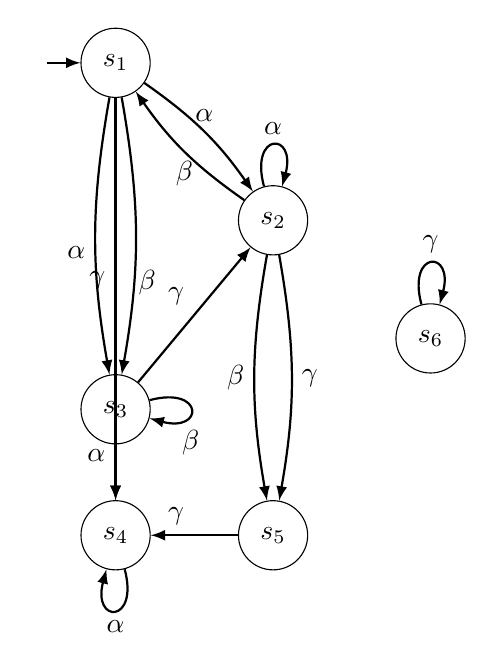
\begin{tikzpicture} [scale=2, every initial by arrow/.style={thick}]
		

		\path
		(\basex,		\basey) 		node[state,init] (s1) 	{$\state_1$} 
		(\basex+2,		\basey+0) 		node[state] (s2) 	{$\state_2$} 
		(\basex+1,		\basey-1.2) 	node[state] (s3) 	{$\state_3$} 
		(\basex,		\basey-2) 		node[state] (s4) 	{$\state_4$} 
		(\basex+2,		\basey-2) 		node[state] (s5) 	{$\state_5$}
		(\basex+3,		\basey-.75) 	node[state] (s6) 	{$\state_6$}
				
		;
		
%		
		\path [bendtrans] 	(s1) 	edge node [midway,above]				{\action} 		(s2);
		\path [bendtrans] 	(s1) 	edge node [near end,above right=-2pt]	{\actionb} 		(s3);
		\path [bendtransr] 	(s1) 	edge node [midway,below left]	{\action} 		(s3);
		\path [trans] 		(s1) 	edge node [midway,above left]	{\actionc} 		(s4);
		\path [bendtrans] 	(s2) 	edge node [midway,below]		{\actionb} 		(s1);
		\path [bendtransr] 	(s2) 	edge node [midway,left]			{\actionb} 		(s5);
		\path [bendtrans] 	(s2) 	edge node [midway,right]		{\actionc} 		(s5);
		\path [trans] 		(s3)	edge node [midway,above left]	{\actionc} 		(s2);
		\path [trans] 		(s3)	edge node [midway,above left]	{\action} 		(s4);
		\path [trans] 		(s5)	edge node [midway,above left]	{\actionc} 		(s4);
		
		\path [trans] 		(s2) 	edge [loop above] node [midway,above] {\action} 	(s2);
		\path [trans] 		(s3) 	edge [loop right] node [midway,below=4pt] {\actionb} 	(s3);
		\path [trans] 		(s4) 	edge [loop below] node [midway,below] {\action} 	(s4);
		\path [trans] 		(s6) 	edge [loop above] node [midway,above] {\actionc} 	(s6);
		
		
		%		midway, at start, near start, very near start, at end, near end, very near end
		
		
	\end{tikzpicture}
\end{document}
	\end{minipage}%
	\begin{minipage}{.5\textwidth}						
		\centering
		\documentclass[tikz,preview]{standalone}
%\usepackage{prelude}

%%%%%%%%%%%%%%%%%%%%%%%%%%%%%%%%%%%% PACKAGES %%%%%%%%%%%%%%%%%%%%%%%%%%%%%%%%%%%%%%%%%%

\usepackage{inputenc,fontenc}
\usepackage[a4paper,margin=3cm]{geometry}
\usepackage[english]{babel}
%\usepackage[german]{babel}
%\usepackage[fixlanguage]{babelbib}


\usepackage{bbold}
\usepackage{amsthm}
\usepackage{amsmath}
\usepackage{amssymb} % doteqdot
\usepackage[dvipsnames]{xcolor}
\usepackage{standalone}
\usepackage{tikz}[mode=buildnew]
\usepackage{cite}
\usepackage{xspace}
\usepackage{relsize}
\usepackage{mathtools} % mathclap
%\usepackage{MnSymbol}
\usepackage{hyperref}
\usepackage{url}
\usepackage{listings} % for code
\usepackage[T1]{fontenc} %<
\hypersetup{
	colorlinks,
	citecolor=black,
	filecolor=black,
	linkcolor=black,
	urlcolor=black
}
\usepackage{pgfplots}
\pgfplotsset{compat=1.18}
%\usepackage{courier} %% Sets font for listing as Courier. But also for url and texttt!
\usepackage{listings, xcolor}
\usepackage{graphicx}
\usepackage{subcaption}

\usetikzlibrary{calc}
%\usepackage{xparse} % \newDocumentCommand for multiple optional arguments
%\usepackage{titlecaps}



%%%%%%%%%%%%%%%%%%%%%%%%%%%%%%%%%%%% THEOREMSTYLES %%%%%%%%%%%%%%%%%%%%%%%%%%%%%%%%%%

\theoremstyle{definition}
\newtheorem{definition}{Definition}[section]
\newtheorem{exmp}{Beispiel}[section]
%\AfterEndEnvironment{definition}{\noindent\ignorespaces}

\theoremstyle{theorem}
\newtheorem{theorem}{Satz}[section]
\newtheorem{proposition}{Proposition}[section]
%\AfterEndEnvironment{theorem}{\noindent\ignorespaces}

\theoremstyle{korollary}
\newtheorem{korollary}{Korollar}[section]
%\AfterEndEnvironment{korollary}{\noindent\ignorespaces}


\tikzset{
	mstate/.style={draw, circle, minimum size=.94cm}, 
	gstate/.style={draw, rectangle, minimum size=.8cm},
	varstate/.style={draw,rectangle, rounded corners, minimum size=1}, 
	trans/.style={draw, ->, thick},
	bendtrans/.style={draw, ->, thick, bend left=10},
	bendtransr/.style={draw, ->, thick, bend right=10},
	init/.style={initial, initial distance=6pt, initial text=},
	every loop/.style={min distance=5pt, looseness=8},
	>=latex
}
\usetikzlibrary{automata,positioning}

%auto shift/.style={auto=right,->,
%	to path={ let \p1=(\tikztostart),\p2=(\tikztotarget),
%		\n1={atan2(\y2-\y1,\x2-\x1)},\n2={\n1+180}
%		in ($(\tikztostart.{\n1})!1mm!270:(\tikztotarget.{\n2})$) -- 
%		($(\tikztotarget.{\n2})!1mm!90:(\tikztostart.{\n1})$) \tikztonodes}},

%%%%%%%%%%%%%%%%%%%%%%%%%%%%%%%%%%% MY MACROS %%%%%%%%%%%%%%%%%%%%%%%%%%%%%%%%%%%%%%%%%
%formatting
\newcommand{\comment}[2]{{\color{#1}#2}}
\newcommand{\redcomment}[1]{{\color{red}#1}}
\newcommand{\purpcomment}[1]{{\color{pink}#1}}
\newcommand{\bluecomment}[1]{{\color{blue}#1}}
\newcommand{\mt}[1]{\ensuremath{{#1}}\xspace}
\newcommand{\mynewcommand}[2]{\newcommand{#1}{\mt{#2}}} %% currently not used becaue of ide highlighting
\newcommand{\arr}{\mt{\to}}

%model checking terms
\newcommand{\mimicrel}{\mt{\mathcal{R}}}
\newcommand{\bisimeq}{\mt{\;\!\sim\;\!}}
\newcommand{\simorder}{\mt{\;\!\preceq\;\!}}
\newcommand{\simequiv}{\mt{\;\!\simeq\;\!}} %command already defined
\newcommand{\relts}{\mt{\;\!\bullet_{_{\tiny{TS}}}\;\!}}
\newcommand{\rel}{\mt{\;\!\bullet\;\!}}

%own names
\newcommand{\nm}[1]{#1\xspace}
\newcommand{\mdpN}{\nm{MDP}}
\newcommand{\mdpsN}{\nm{MDPs}}
\newcommand{\viewN}{\nm{view}}
\newcommand{\viewNC}{\nm{View}}
\newcommand{\viewsN}{\nm{views}}
\newcommand{\viewsNC}{\nm{Views}}
\newcommand{\grpfctsubN}{\nm{detached grouping function}}
\newcommand{\grpfctsubNC}{\nm{detached grouping function}}
\newcommand{\grpfctsubNCC}{\nm{Detached Grouping Function}}
\newcommand{\grpfctN}{\nm{grouping function}}
\newcommand{\grpfctNC}{\nm{Grouping function}}
\newcommand{\grpfctNCC}{\nm{Grouping Function}}
\newcommand{\grpfctsN}{\nm{grouping functions}}
\newcommand{\grpfctsNC}{\nm{Grouping functions}}
\newcommand{\grpfctsNCC}{\nm{Grouping Functions}}
\newcommand{\stmimicN}{\nm{state-mimic}}
\newcommand{\stmimicsN}{\nm{state-mimics}}
\newcommand{\stmimickingN}{\nm{state-mimicking}}
\newcommand{\stmimickedN}{\nm{state-mimicked}}
%\newcommand{\chosenphtypeNCC}{\nm{Transition System}}
%\newcommand{\chgphNC}{\nm{Transition system}}
%\newcommand{\chgphN}{\nm{transition system}}
%\newcommand{\chgphsNCC}{\nm{Transition Systems}}
%\newcommand{\chgphsNC}{\nm{Transition systems}}
%\newcommand{\chgphsN}{\nm{transition systems}}
\newcommand{\chgphNCC}{\nm{MDP}}
\newcommand{\chgphNC}{\nm{MDP}}
\newcommand{\chgphN}{\nm{MDP}}
\newcommand{\achgphN}{\nm{an MDP}}
\newcommand{\chgphsNCC}{\nm{MDPs}}
\newcommand{\chgphsNC}{\nm{MDPs}}
\newcommand{\chgphsN}{\nm{MDPs}}
\newcommand{\parllcompN}{\nm{parallel composition}}
\newcommand{\parllcompNC}{\nm{Parallel composition}}
\newcommand{\parllcompNCC}{\nm{Parallel Composition}}
\newcommand{\parllcompsN}{\nm{parallel compositions}}
\newcommand{\parllcompsNC}{\nm{Parallel compositions}}
\newcommand{\parllcompsNCC}{\nm{Parallel Compositions}}
\newcommand{\sccN}{\nm{SCC}}
\newcommand{\sccsN}{\nm{SCCs}}
\newcommand{\bsccN}{\nm{BSCC}}
\newcommand{\bsccsN}{\nm{BSCCs}}
\newcommand{\jgrapht}{\nm{jGraphtT}}

\newcommand{\outactident}{\nm{OutActionsIdent}}

%names
\newcommand{\iffN}{\nm{if and only if}}
\newcommand{\tsN}{\nm{TS}}

%% outactions identical
\newcommand{\outactidentstrong}{\nm{strong}}
\newcommand{\outactidentweak}{\nm{weak}}

% CORE DEFINITIONS
\newcommand{\grpfct}[1][\viewppty]{\mt{F_{#1}}}
\newcommand{\grpfctsub}[1][\viewppty]{\mt{\tilde{F}_{#1}}}
%\newcommand{\grpfctimg}[1]{\mt{{\grpfct}[{#1}]}}
%\newcommand{\fctimg}[2]{\mt{{#1}[{#2}]}}
\newcommand{\eqrelview}{\mt{R}}
\newcommand{\eqclassv}[1][\state]{\mt{\eqclass{#1}{\eqrelview}}}
\newcommand{\eqclasssetv}[1][\states]{\mt{{#1}/\eqrelview}} %OLD: \bigcup_{\state \in \states} \eqclassv
\newcommand{\viewid}{\mt{\mdp}}
\newcommand{\view}[1][\viewppty]{\mt{\viewid_{#1}}}
\newcommand{\imggrp}{\mt{\arbset}}
\newcommand{\imggrpsub}{\mt{X}}
\newcommand{\viewppty}{\mt{\theta}}
\newcommand{\pll}{\mt{\;\!\pllpure\;\!}}
\newcommand{\pllrev}{\mt{\pllpure^{-1}}}
\newcommand{\pllpure}{\mt{||}}
\newcommand{\compselectset}{\mt{Z}}
\newcommand{\compselectpure}{\mt{\pllpure_\compselectset}}
\newcommand{\compselect}{\mt{\;\pllpure_\compselectset\;}}
\newcommand{\remstates}{\mt{\bigcup_{\state \in \states \setminus \states_1}\{\{\state\}\}}}
\newcommand{\nogroupstates}[1][\states_2]{\mt{\bigcup_{\state \in \states \setminus {#1}}\{\{\state\}\}}}
\newcommand{\remelem}{\mt{\bullet}}
\newcommand{\nogroupset}{\mt{\xi}}
\newcommand{\remset}{\mt{\{\remelem\}}}
\newcommand{\gfctpll}{\mt{\grpfct[\pll]}}
\newcommand{\group}{\mt{\top}}
\newcommand{\imggrpbinview}{\mt{\{\remelem, \notppty\}}}
\newcommand{\viewappset}{\mt{\tilde{\states}}}
\newcommand{\hasppty}{\mt{\top}}
\newcommand{\notppty}{\mt{\bot}}
\newcommand{\disregardelem}{\mt{\Delta}}
\newcommand{\disregardelements}{\mt{{\disregardelem_1, \dots, \disregardelem_n}}}



%\newcommand{\mdp}{def}\mdp
%\newcommand{\mdpdef}



% EXAMPLE VIEWS
\newcommand{\pptyatomicprops}{\mt{\atomicprops}}
\newcommand{\pptyinitstates}{\mt{\initstates}}
\newcommand{\pptyinactsetsize}{\mt{|\inacts(\state)|}}
\newcommand{\pptyhasoutact}{\mt{\exists\outact}}
\newcommand{\pptyminoutact}[2]{\mt{#1\leq#2}}
\newcommand{\pptymaxoutact}[2]{\mt{#2\leq#1}}
\newcommand{\pptyspanoutact}[3]{\mt{#1\leq#2\leq#3}}
\newcommand{\pptyoutactsetsize}{\mt{|\outacts(\state)|}}
\newcommand{\pptyoutactsingle}{\mt{|\outacts(\state)|_1}}
\newcommand{\pptystrongoutactident}{\mt{\outacts(\state)_=}}
\newcommand{\pptyweakoutactident}{\mt{\outacts(\state)_\approx}}
\newcommand{\pptyhasinact}{\mt{\exists\inact}}
\newcommand{\pptymininact}[2]{\mt{#1\leq#2}}
\newcommand{\pptymaxinact}[2]{\mt{#2\leq#1}}
\newcommand{\pptyspaninact}[3]{\mt{#1\leq#2\leq#3}}
\newcommand{\pptyinactsingle}{\mt{|\inacts(\state)|_1}}
\newcommand{\pptystronginactident}{\mt{\inacts(\state)_=}}
\newcommand{\pptyweakinactident}{\mt{\inacts(\state)_\approx}}
\newcommand{\pptyparamvalueseq}{\mt{\var = \varval}}
\newcommand{\pptyparamvaluesneq}{\mt{\var \neq \varval}}
\newcommand{\pptyparamdnf}{\mt{VarDNF}}
\newcommand{\pptyparamcnf}{\mt{VarCNF}}
\newcommand{\pptyparamvalueseqopt}{\mt{\var = \varval}}
\newcommand{\pptyparamvalident}{\mt{Var:\varval}}
\newcommand{\pptydistance}{\mt{\distpath}}
\newcommand{\pptydistancerev}{\mt{\distpathrev}}
\newcommand{\pptydistancebi}{\mt{\distpathbi}}
\newcommand{\pptyhascycle}{\mt{\exists\cycle}}
\newcommand{\pptyexactactcycle}{\mt{\{\cycle_{\action,n}\}}}
\newcommand{\pptycycleset}{\mt{\cup{\{\state\}_\cycle}}}
\newcommand{\pptyexactcycle}{\mt{\{\cycle_n\}}}
\newcommand{\pptyscc}{\mt{scc}}
\newcommand{\pptybscc}{\mt{bscc}}
\newcommand{\pptyprop}{\mt{\redcomment{?}}}
\newcommand{\pptyident}{id}


\newcommand{\gfctatomicprops}{\mt{\grpfct[\pptyatomicprops]}}
\newcommand{\gfctinitstates}{\mt{\grpfct[\pptyinitstates]^\hasppty}}
\newcommand{\gfcthasoutaction}{\mt{\grpfct[\pptyhasoutact]^\hasppty}}
\newcommand{\gfctminoutaction}{\mt{\grpfct[\pptyminoutact{\numoutact}{\outact}]^\hasppty}}
\newcommand{\gfctmaxoutaction}{\mt{\grpfct[\pptymaxoutact{\numoutact}{\outact}]^\hasppty}}
\newcommand{\gfctspanoutaction}{\mt{\grpfct[\pptyspanoutact{\numoutactb}{\outact}{\numoutact}]^\hasppty}}
\newcommand{\gfctoutactsetsize}{\mt{\grpfct[\pptyoutactsetsize]}}
\newcommand{\gfctoutactsingle}{\mt{\grpfct[\pptyoutactsingle]^\notppty}}
\newcommand{\gfctstrongoutactident}{\mt{\grpfct[\pptystrongoutactident]}}
\newcommand{\gfctweakoutactident}{\mt{\grpfct[\pptyweakoutactident]}}
\newcommand{\gfcthasinaction}{\mt{\grpfct[\pptyhasinact]^\hasppty}}
\newcommand{\gfctmininaction}{\mt{\grpfct[\pptymininact{\numinact}{\inact}]^\hasppty}}
\newcommand{\gfctmaxinaction}{\mt{\grpfct[\pptymaxinact{\numinact}{\inact}]^\hasppty}}
\newcommand{\gfctspaninaction}{\mt{\grpfct[\pptyspaninact{\numinactb}{\inact}{\numinact}]^\hasppty}}
\newcommand{\gfctinactsetsize}{\mt{\grpfct[\pptyinactsetsize]}}
\newcommand{\gfctinactsingle}{\mt{\grpfct[\pptyinactsingle]^\notppty}}
\newcommand{\gfctstronginactident}{\mt{\grpfct[\pptystronginactident]}}
\newcommand{\gfctweakinactident}{\mt{\grpfct[\pptyweakinactident]}}
\newcommand{\gfctparamvalueseq}{\mt{\grpfct[\pptyparamvalueseq]^\hasppty}}
\newcommand{\gfctparamvaluesneq}{\mt{\grpfct[\pptyparamvaluesneq]^\hasppty}}
\newcommand{\gfctparamdnf}{\mt{\grpfct[\pptyparamdnf]^\hasppty}}
\newcommand{\gfctparamcnf}{\mt{\grpfct[\pptyparamcnf]^\hasppty}}
\newcommand{\gfctparamvalueseqopt}{\mt{\pptyparamvalueseqopt}}
\newcommand{\gfctparamvalident}{\mt{\grpfct[\pptyparamvalident]}}
\newcommand{\gfctdistance}{\mt{\grpfct[\pptydistance]}}
\newcommand{\gfctdistancerev}{\mt{\grpfct[\pptydistancerev]}}
\newcommand{\gfctdistancebi}{\mt{\grpfct[\pptydistancebi]}}
\newcommand{\gfcthascycle}{\mt{\grpfct[\pptyhascycle]}}
\newcommand{\gfctexactcycle}{\mt{\grpfct[\pptyexactcycle]}}
\newcommand{\gfctcycleset}{\mt{\grpfct[\pptycycleset]}}
\newcommand{\gfctexactactcycle}{\mt{\grpfct[\pptyexactactcycle]}}
\newcommand{\gfctscc}{\mt{\grpfct[\pptyscc]}}
\newcommand{\gfctbscc}{\mt{\grpfct[\pptybscc]}}
\newcommand{\gfctprop}{\mt{\grpfct[\pptyprop]}}
\newcommand{\gfctident}{\mt{\grpfct[\pptyident]}}

\newcommand{\gfctsubatomicprops}{\mt{\grpfctsub[\pptyatomicprops]}}
\newcommand{\gfctsubinitstates}{\mt{\grpfctsub[\pptyinitstates]^\hasppty}}
\newcommand{\gfctsubhasoutaction}{\mt{\grpfctsub[\pptyhasoutact]^\hasppty}}
\newcommand{\gfctsubminoutaction}{\mt{\grpfctsub[\pptyminoutact{\numoutact}{\outact}]^\hasppty}}
\newcommand{\gfctsubmaxoutaction}{\mt{\grpfctsub[\pptymaxoutact{\numoutact}{\outact}]^\hasppty}}
\newcommand{\gfctsubspanoutaction}{\mt{\grpfctsub[\pptyspanoutact{\numoutactb}{\outact}{\numoutact}]^\hasppty}}
\newcommand{\gfctsuboutactsetsize}{\mt{\grpfctsub[\pptyoutactsetsize]}}
\newcommand{\gfctsuboutactsingle}{\mt{\grpfctsub[\pptyoutactsingle]^\notppty}}
\newcommand{\gfctsubstrongoutactident}{\mt{\grpfctsub[\pptystrongoutactident]^\hasppty}}
\newcommand{\gfctsubweakoutactident}{\mt{\grpfctsub[\pptyweakoutactident]^\hasppty}}
\newcommand{\gfctsubhasinaction}{\mt{\grpfctsub[\pptyhasinact]}}
\newcommand{\gfctsubmininaction}{\mt{\grpfctsub[\pptymininact{\numinact}{\inact}]}}
\newcommand{\gfctsubmaxinaction}{\mt{\grpfctsub[\pptymaxinact{\numinact}{\inact}]}}
\newcommand{\gfctsubspaninaction}{\mt{\grpfctsub[\pptyspaninact{\numinactb}{\inact}{\numinact}]}}
\newcommand{\gfctsubinactsetsize}{\mt{\grpfctsub[\pptyinactsetsize]^\hasppty}}
\newcommand{\gfctsubinactsingle}{\mt{\grpfctsub[\pptyinactsingle]^\notppty}}
\newcommand{\gfctsubstronginactident}{\mt{\grpfctsub[\pptystronginactident]}}
\newcommand{\gfctsubweakinactident}{\mt{\grpfctsub[\pptyweakinactident]}}
\newcommand{\gfctsubparamvalueseq}{\mt{\grpfctsub[\pptyparamvalueseq]^\hasppty}}
\newcommand{\gfctsubparamvaluesneq}{\mt{\grpfctsub[\pptyparamvaluesneq]^\hasppty}}
\newcommand{\gfctsubparamdnf}{\mt{\grpfctsub[\pptyparamdnf]^\hasppty}}
\newcommand{\gfctsubparamcnf}{\mt{\grpfctsub[\pptyparamcnf]^\hasppty}}
\newcommand{\gfctsubparamvalueseqopt}{\mt{\pptyparamvalueseqopt}}
\newcommand{\gfctsubparamvalident}{\mt{\grpfctsub[\pptyparamvalident]}}
\newcommand{\gfctsubdistance}{\mt{\grpfctsub[\pptydistance]}}
\newcommand{\gfctsubdistancerev}{\mt{\grpfctsub[\pptydistancerev]}}
\newcommand{\gfctsubdistancebi}{\mt{\grpfctsub[\pptydistancebi]}}
\newcommand{\gfctsubhascycle}{\mt{\grpfctsub[\pptyhascycle]^\hasppty}}
\newcommand{\gfctsubexactcycle}{\mt{\grpfctsub[\pptyexactcycle]}}
\newcommand{\gfctsubcycleset}{\mt{\grpfctsub[\pptycycleset]}}
\newcommand{\gfctsubexactactcycle}{\mt{\grpfctsub[\pptyexactactcycle]}}
\newcommand{\gfctsubscc}{\mt{\grpfctsub[\pptyscc]}}
\newcommand{\gfctsubbscc}{\mt{\grpfctsub[\pptybscc]}}
\newcommand{\gfctsubprop}{\mt{\grpfctsub[\pptyprop]}}
\newcommand{\gfctsubident}{\mt{\grpfctsub[\pptyident]}}


\newcommand{\viewatomicprops}{\mt{\view[\pptyatomicprops]}}
\newcommand{\viewinitstates}{\mt{\view[\pptyinitstates]^\hasppty}}
\newcommand{\viewhasoutaction}{\mt{\view[\pptyhasoutact]^\hasppty}}
\newcommand{\viewminoutaction}{\mt{\view[\pptyminoutact{\numoutact}{\outact}]^\hasppty}}
\newcommand{\viewmaxoutaction}{\mt{\view[\pptymaxoutact{\numoutact}{\outact}]^\hasppty}}
\newcommand{\viewspanoutaction}{\mt{\view[\pptyspanoutact{\numoutactb}{\outact}{\numoutact}]^\hasppty}}
\newcommand{\viewoutactsetsize}{\mt{\view[\pptyoutactsetsize]}}
\newcommand{\viewoutactsingle}{\mt{\view[\pptyoutactsingle]^\notppty}}
\newcommand{\viewstrongoutactident}{\mt{\view[\pptystrongoutactident]}}
\newcommand{\viewweakoutactident}{\mt{\view[\pptyweakoutactident]}}
\newcommand{\viewhasinaction}{\mt{\view[\pptyhasinact]^\hasppty}}
\newcommand{\viewmininaction}{\mt{\view[\pptymininact{\numinact}{\inact}]^\hasppty}}
\newcommand{\viewmaxinaction}{\mt{\view[\pptymaxinact{\numinact}{\inact}]^\hasppty}}
\newcommand{\viewspaninaction}{\mt{\view[\pptyspaninact{\numinactb}{\inact}{\numinact}]^\hasppty}}
\newcommand{\viewinactsetsize}{\mt{\view[\pptyinactsetsize]}}
\newcommand{\viewinactsingle}{\mt{\view[\pptyinactsingle]^\notppty}}
\newcommand{\viewstronginactident}{\mt{\view[\pptystronginactident]}}
\newcommand{\viewweakinactident}{\mt{\view[\pptyweakinactident]}}
\newcommand{\viewparamvalueseq}{\mt{\view[\pptyparamvalueseq]}}
\newcommand{\viewparamvaluesneq}{\mt{\view[\pptyparamvaluesneq]}}
\newcommand{\viewparamdnf}{\mt{\view[\pptyparamdnf]^\hasppty}}
\newcommand{\viewparamcnf}{\mt{\view[\pptyparamcnf]^\hasppty}}
\newcommand{\viewparamvalueseqopt}{\mt{\pptyparamvalueseqopt}}
\newcommand{\viewparamvalident}{\mt{\view[\pptyparamvalident]}}
\newcommand{\viewdistance}{\mt{\view[\pptydistance]}}
\newcommand{\viewdistancerev}{\mt{\view[\pptydistancerev]}}
\newcommand{\viewdistancebi}{\mt{\view[\pptydistancebi]}}
\newcommand{\viewhascycle}{\mt{\view[\pptyhascycle]}}
\newcommand{\viewexactcycle}{\mt{\view[\pptyexactcycle]}}
\newcommand{\viewcycleset}{\mt{\view[\pptycycleset]}}
\newcommand{\viewexactactcycle}{\mt{\view[\pptyexactactcycle]}}
\newcommand{\viewscc}{\mt{\view[\pptyscc]}}
\newcommand{\viewbscc}{\mt{\view[\pptybscc]}}
\newcommand{\viewprop}{\mt{\view[\pptyprop]}}
\newcommand{\viewident}{\mt{\view[\pptyident]}}

%\newcommand{\viewatomicprops}{\mt{\view[\atomicprops]}}
%\newcommand{\viewinitstates}{\mt{\view[\initstates]}}
%\newcommand{\viewhasoutaction}{\mt{\view[\pptyhasoutact]}}
%\newcommand{\viewminoutaction}{\mt{\view[\pptyminoutact{\numoutact}{\outact}]}}
%\newcommand{\viewmaxoutaction}{\mt{\view[\pptymaxoutact{\numoutact}{\outact}]}}
%\newcommand{\viewspanoutaction}{\mt{\view[\pptyspanoutact{\numoutactb}{\outact}{\numoutact}]}}
%\newcommand{\viewoutactsetsize}{\mt{\view[\pptyoutactsetsize]}}
%\newcommand{\viewoutactsingle}{\mt{\view[\pptyoutactsingle]}}
%\newcommand{\viewstrongoutactident}{\mt{\view[\outacts(\state)_=]}}
%\newcommand{\viewweakoutactident}{\mt{\view[\outacts(\state)_\approx]}}
%\newcommand{\viewhasinaction}{\mt{\view[\pptyhasinact]}}
%\newcommand{\viewmininaction}{\mt{\view[\pptymininact{\numinact}{\inact}]}}
%\newcommand{\viewmaxinaction}{\mt{\view[\pptymaxinact{\numinact}{\inact}]}}
%\newcommand{\viewspaninaction}{\mt{\view[\pptyspaninact{\numinactb}{\inact}{\numinact}]}}
%\newcommand{\viewinactsetsize}{\mt{\view[\pptyinactsetsize]}}
%\newcommand{\viewinactsingle}{\mt{\view[\pptyinactsingle]}}
%\newcommand{\viewstronginactident}{\mt{\view[\inacts(\state)_=]}}
%\newcommand{\viewweakinactident}{\mt{\view[\inacts(\state)_\approx]}}
%\newcommand{\viewparamvalueseq}{\mt{\view[\var = \varval]}}
%\newcommand{\viewparamvaluesneq}{\mt{\view[\var \neq \varval]}}
%\newcommand{\viewparamdnf}{\mt{\view[VarDNF]}}
%\newcommand{\viewparamcnf}{\mt{\view[VarCNF]}}
%\newcommand{\viewparamvalident}{\mt{\view[\pptyparamvalident]}}
%\newcommand{\viewdistance}{\mt{\view[\pptydistance]}}
%\newcommand{\viewhascycle}{\mt{\view[\exists\cycle]}}
%\newcommand{\viewexactcycle}{\mt{\view[\pptyexactcycle]}}
%\newcommand{\viewcycleset}{\mt{\view[\pptycycleset]}}
%\newcommand{\viewexactactcycle}{\mt{\view[\pptyexactactcycle]}}
%\newcommand{\viewscc}{\mt{\view[scc]}}
%\newcommand{\viewbscc}{\mt{\view[bscc]}}

%actions
\newcommand{\numoutact}{\mt{n}}
\newcommand{\numoutactb}{\mt{m}}
\newcommand{\numinact}{\mt{n}}
\newcommand{\numinactb}{\mt{m}}

\newcommand{\predmaxoutact}[1][\numoutact]{\mt{Q_{\outact\leq#1}(\state,\state_1, \dots, \state_{#1+1})}}
\newcommand{\predminoutact}[1][\numoutact]{\mt{Q_{#1\leq\outact}(\state,\state_1, \dots, \state_{#1})}}
\newcommand{\formoutact}[1][\state]{\mt{C_{#1,\outact}}}
\newcommand{\predmaxinact}[1][\numinact]{\mt{Q_{\inact\leq#1}(\state,\state_1, \dots, \state_{#1+1})}}
\newcommand{\predmininact}[1][\numinact]{\mt{Q_{#1\leq\inact}(\state,\state_1, \dots, \state_{#1})}}

\newcommand{\outact}[1][\action]{\mt{\overrightarrow{#1}}}
\newcommand{\outacts}{\mt{\overrightarrow{\actions}}}
\newcommand{\inact}{\mt{\overleftarrow{\action}}}
\newcommand{\inacts}[1][\action]{\mt{\overleftarrow{#1}}}

%%Parameters
\newcommand{\vars}[1][\mdp]{\mt{V\!ar_{#1}}}
\newcommand{\var}{\mt{x}}
\newcommand{\varstate}[1][]{\mt{\var_{\state#1}}}
\newcommand{\varval}{\mt{a}}
\newcommand{\vareval}[1][\mdp]{\mt{V\!arEval_{#1}}}
\newcommand{\varevalimg}[1][\mdp]{\mt{\vareval[#1][\states,\vars]}}
\newcommand{\varevalimgset}{\mt{\arbset}}
\newcommand{\someparam}{\mt{\tilde{x}}}
\newcommand{\eqorneq}{\mt{\;\doteqdot\;}}
\newcommand{\varstyle}[2]{\mt{\langle#1,#2\rangle}}




%\makeatletter
%\newcommand{\overleftrightsmallarrow}{\mathpalette{\overarrowsmall@\leftrightarrowfill@}}
%\newcommand{\overrightsmallarrow}{\mathpalette{\overarrowsmall@\rightarrowfill@}}
%\newcommand{\overleftsmallarrow}{\mathpalette{\overarrowsmall@\leftarrowfill@}}
%\newcommand{\overarrowsmall@}[3]{%
%	\vbox{%
%		\ialign{%
%			##\crcr
%			#1{\smaller@style{#2}}\crcr
%			\noalign{\nointerlineskip}%
%			$\m@th\hfil#2#3\hfil$\crcr
%		}%
%	}%
%}
%\def\smaller@style#1{%
%	\ifx#1\displaystyle\scriptstyle\else
%	\ifx#1\textstyle\scriptstyle\else
%	\scriptscriptstyle
%	\fi
%	\fi
%}
%\makeatother
%\newcommand{\te}[1]{\overleftrightsmallarrow{#1}}

% Distance
\newcommand{\fctdist}{\mt{distance}}
\newcommand{\fctdistdefault}{\mt{\fctdist(\chgph, \smstates, \grandist)}}
\newcommand{\distval}{\mt{d}}
\newcommand{\grandist}{\mt{n}}
\let\path\oldpath
\newcommand{\path}{\mt{P}}
\newcommand{\pathbi}{\mt{\bar{\path}}}
\newcommand{\pathsecfull}{\mt{(\state_0, \action_0, \state_1, \action_1, \dots, \action_{n}, \state_{n+1})}}
\newcommand{\lenpath}{\mt{len}}
\newcommand{\pfirst}{\mt{first}}
\newcommand{\plast}{\mt{last}}
\newcommand{\pathset}{\mt{\path_\chgph}}
\newcommand{\pathbiset}{\mt{\pathbi_\chgph}}
\newcommand{\distpath}{\mt{\overrightarrow{dist}}}
\newcommand{\distpathrev}{\mt{\overleftarrow{dist}}}
\newcommand{\distpathbi}{\mt{\overline{dist}}}
%Cycles
\newcommand{\cyclesecfull}{\mt{(\state_0, \action_0, \state_1, \action_1, \dots, \action_{n-1}, \state_0)}}
\newcommand{\fctfindcycles}{\mt{findCycles}}
\newcommand{\cycle}{\mt{C}}
\newcommand{\cycleset}{\mt{\cycle_{\mdp, n}}}
\newcommand{\lencycle}{\mt{len}}
% strongly connected components
\newcommand{\scc}{\mt{T}}
\newcommand{\setscc}{\mt{SCC_{\chgph,n}}}
\newcommand{\setbscc}{\mt{BSCC_{\chgph,n}}}

% properties
\newcommand{\propfct}{\mt{f}}

% all Systems
\newcommand{\chgph}{\mt{\mdp}}
\newcommand{\chgphtuple}{\mt{\mdptuple}}
\newcommand{\chgphtupledist}{\mt{\mdptupledist}}

\newcommand{\states}{\mt{S}}
\newcommand{\actions}{\mt{Act}}
\newcommand{\atomicprops}{\mt{AP}}
\newcommand{\labelingfct}{\mt{L}}
\newcommand{\init}{\mt{\initdistrib}} % use MDP % refers to the underlying set
\newcommand{\trans}{\mt{\probtfunc}} % use MDP % refers to the underlying set
\newcommand{\smstates}{\mt{\tilde{\states}}}


\newcommand{\state}{\mt{s}}
\newcommand{\action}{\mt{\alpha}}
\newcommand{\actionb}{\mt{\beta}}
\newcommand{\actionc}{\mt{\gamma}}
\newcommand{\smstate}{\mt{\tilde{\state}}}



% transition sysstems
\newcommand{\ts}{\mt{TS}}
\newcommand{\transitionrel}{\mt{\longrightarrow}}
\newcommand{\initstates}{\mt{I}}
\newcommand{\transitionsystem}{\mt
	{(\states, \actions, \transitionrel, \initstates, \atomicprops, \labelingfct)}
}
\newcommand{\tstupledist}{\mt{(\states', \actions',\transitionrel', \initstates', \labelingfct')}}


%Markov chains and MDP
\newcommand{\mdp}{\mt{\autm}}
\newcommand{\mdptuple}{\mt{(\states, \actions, \probtfunc, \initdistrib, \atomicprops, \labelingfct)}}
\newcommand{\mdptupledist}{\mt{(\states', \actions', \probtfunc', \initdistrib', \atomicprops', \labelingfct')}}
\newcommand{\autm}{\mt{\mathcal{M}}}
\newcommand{\probtfunc}{\mt{\textbf{P}}}
\newcommand{\initdistrib}{\mt{\iota_{init}}}


%maths
\newcommand{\powerset}[1]{\mt{\mathcal{P}(#1)}}
\newcommand{\eqclass}[2]{\mt{[#1]_{#2}}}%{\mt{#1 / #2}}
\newcommand{\impr}{\mt{\hspace{3mm}\Rightarrow\hspace{2mm}}}
\newcommand{\impl}{\mt{\hspace{3mm}\Leftarrow\hspace{2mm}}}
\newcommand{\natnums}{\mt{\mathbb{N}}} 
\newcommand{\realnums}{\mt{\mathbb{R}}}
\newcommand{\intmodn}[1][n]{\mt{\mathbb{Z}_{#1}}}
\newcommand{\arbset}{\mt{M}}
\newcommand{\bigsum}[2][]{\mt{\mathlarger{\sum}_{#2}^{#1}}}
\newcommand{\bbigsum}[2][]{\mt{\mathlarger{\mathlarger{\sum}}_{#2}^{#1}}}
\newcommand{\invimage}[2]{#1^{\mt{-1}(#2)}}
\newcommand{\img}{\mt{Img}}
\newcommand{\cond}{\mt{\,|\,}}

%tickz
%% \definecolor{darkred}{RGB}{196, 42, 42}

%implementation
\newcommand{\pmcvis}{\nm{PMC-Vis}}


\begin{document}
	\newcommand{\basex}{0}
	\newcommand{\basey}{0}
	\newcommand{\createstate}[3]{\node[draw, circle, minimum size=1cm] (#1) at (#2) {#3}}
	
	
	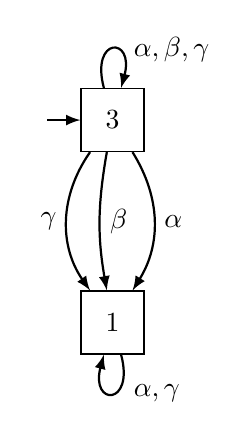
\begin{tikzpicture} [scale=2, every initial by arrow/.style={thick}]
		
		
		\node [gstate,init] (set3) at (0,0) {$3$};
		\node [gstate,below=50pt of set3] (set1) {$1$};
		
		\path [trans,bend right=35] (set3) edge node [midway, left] {\actionc} (set1);
		\path [trans,bend right=10] (set3) edge node [midway, right] {\actionb} (set1);
		\path [trans,bend left=32] (set3) edge node [midway, right] {\action} (set1);
		
		\path [trans] (set3) edge [loop above] node [midway, right=4pt] {$\action,\actionb,\actionc$} (set3);
		\path [trans] (set1) edge [loop below] node [midway, right=4pt] {$\action,\actionc$} (set1);
		

		
		
	\end{tikzpicture}
\end{document}
	\end{minipage}	
	\caption{Simplified representations of \mdp (left) and the \viewN \viewoutactsetsize on it (right)}	
	\label{fig:outActSetSize}  	
\end{figure}

The notion of the view is similar to utilize the outdegree, with the difference being here that ougoing transitions with the same action are considered as one single edge. This reflects on the options available for nondeterminism in this state.

The sepcialcase of there only being one single ougoing action is worth a distinct view, since it hides all nondeterministic choices, but nothing more.

\begin{definition}
	Let $\chgph = \chgphtuple$ be \achgphN and $\action \in \actions$. The \viewN \viewoutactsingle is defined by its \grpfctN $\gfctoutactsingle : \states \to \imggrp$ with
	\[\state \mapsto 
	\begin{cases}
		\group, &\text{if } |\{\action \in \actions \mid \exists \state' \in \states : (\state, \action, \state') \in \trans\}| = 1 \\ 
		\remelem, &\text{otherwise}
	\end{cases}
	\]
	and $\imggrp := \natnums \cup \remset$.
\end{definition}

\begin{figure}[h]
	\begin{minipage}{.5\textwidth}
		\hspace{5mm}
		\documentclass[tikz,preview]{standalone}
%\usepackage{prelude}

%%%%%%%%%%%%%%%%%%%%%%%%%%%%%%%%%%%% PACKAGES %%%%%%%%%%%%%%%%%%%%%%%%%%%%%%%%%%%%%%%%%%

\usepackage{inputenc,fontenc}
\usepackage[a4paper,margin=3cm]{geometry}
\usepackage[english]{babel}
%\usepackage[german]{babel}
%\usepackage[fixlanguage]{babelbib}


\usepackage{bbold}
\usepackage{amsthm}
\usepackage{amsmath}
\usepackage{amssymb} % doteqdot
\usepackage[dvipsnames]{xcolor}
\usepackage{standalone}
\usepackage{tikz}[mode=buildnew]
\usepackage{cite}
\usepackage{xspace}
\usepackage{relsize}
\usepackage{mathtools} % mathclap
%\usepackage{MnSymbol}
\usepackage{hyperref}
\usepackage{url}
\usepackage{listings} % for code
\usepackage[T1]{fontenc} %<
\hypersetup{
	colorlinks,
	citecolor=black,
	filecolor=black,
	linkcolor=black,
	urlcolor=black
}
\usepackage{pgfplots}
\pgfplotsset{compat=1.18}
%\usepackage{courier} %% Sets font for listing as Courier. But also for url and texttt!
\usepackage{listings, xcolor}
\usepackage{graphicx}
\usepackage{subcaption}

\usetikzlibrary{calc}
%\usepackage{xparse} % \newDocumentCommand for multiple optional arguments
%\usepackage{titlecaps}



%%%%%%%%%%%%%%%%%%%%%%%%%%%%%%%%%%%% THEOREMSTYLES %%%%%%%%%%%%%%%%%%%%%%%%%%%%%%%%%%

\theoremstyle{definition}
\newtheorem{definition}{Definition}[section]
\newtheorem{exmp}{Beispiel}[section]
%\AfterEndEnvironment{definition}{\noindent\ignorespaces}

\theoremstyle{theorem}
\newtheorem{theorem}{Satz}[section]
\newtheorem{proposition}{Proposition}[section]
%\AfterEndEnvironment{theorem}{\noindent\ignorespaces}

\theoremstyle{korollary}
\newtheorem{korollary}{Korollar}[section]
%\AfterEndEnvironment{korollary}{\noindent\ignorespaces}


\tikzset{
	mstate/.style={draw, circle, minimum size=.94cm}, 
	gstate/.style={draw, rectangle, minimum size=.8cm},
	varstate/.style={draw,rectangle, rounded corners, minimum size=1}, 
	trans/.style={draw, ->, thick},
	bendtrans/.style={draw, ->, thick, bend left=10},
	bendtransr/.style={draw, ->, thick, bend right=10},
	init/.style={initial, initial distance=6pt, initial text=},
	every loop/.style={min distance=5pt, looseness=8},
	>=latex
}
\usetikzlibrary{automata,positioning}

%auto shift/.style={auto=right,->,
%	to path={ let \p1=(\tikztostart),\p2=(\tikztotarget),
%		\n1={atan2(\y2-\y1,\x2-\x1)},\n2={\n1+180}
%		in ($(\tikztostart.{\n1})!1mm!270:(\tikztotarget.{\n2})$) -- 
%		($(\tikztotarget.{\n2})!1mm!90:(\tikztostart.{\n1})$) \tikztonodes}},

%%%%%%%%%%%%%%%%%%%%%%%%%%%%%%%%%%% MY MACROS %%%%%%%%%%%%%%%%%%%%%%%%%%%%%%%%%%%%%%%%%
%formatting
\newcommand{\comment}[2]{{\color{#1}#2}}
\newcommand{\redcomment}[1]{{\color{red}#1}}
\newcommand{\purpcomment}[1]{{\color{pink}#1}}
\newcommand{\bluecomment}[1]{{\color{blue}#1}}
\newcommand{\mt}[1]{\ensuremath{{#1}}\xspace}
\newcommand{\mynewcommand}[2]{\newcommand{#1}{\mt{#2}}} %% currently not used becaue of ide highlighting
\newcommand{\arr}{\mt{\to}}

%model checking terms
\newcommand{\mimicrel}{\mt{\mathcal{R}}}
\newcommand{\bisimeq}{\mt{\;\!\sim\;\!}}
\newcommand{\simorder}{\mt{\;\!\preceq\;\!}}
\newcommand{\simequiv}{\mt{\;\!\simeq\;\!}} %command already defined
\newcommand{\relts}{\mt{\;\!\bullet_{_{\tiny{TS}}}\;\!}}
\newcommand{\rel}{\mt{\;\!\bullet\;\!}}

%own names
\newcommand{\nm}[1]{#1\xspace}
\newcommand{\mdpN}{\nm{MDP}}
\newcommand{\mdpsN}{\nm{MDPs}}
\newcommand{\viewN}{\nm{view}}
\newcommand{\viewNC}{\nm{View}}
\newcommand{\viewsN}{\nm{views}}
\newcommand{\viewsNC}{\nm{Views}}
\newcommand{\grpfctsubN}{\nm{detached grouping function}}
\newcommand{\grpfctsubNC}{\nm{detached grouping function}}
\newcommand{\grpfctsubNCC}{\nm{Detached Grouping Function}}
\newcommand{\grpfctN}{\nm{grouping function}}
\newcommand{\grpfctNC}{\nm{Grouping function}}
\newcommand{\grpfctNCC}{\nm{Grouping Function}}
\newcommand{\grpfctsN}{\nm{grouping functions}}
\newcommand{\grpfctsNC}{\nm{Grouping functions}}
\newcommand{\grpfctsNCC}{\nm{Grouping Functions}}
\newcommand{\stmimicN}{\nm{state-mimic}}
\newcommand{\stmimicsN}{\nm{state-mimics}}
\newcommand{\stmimickingN}{\nm{state-mimicking}}
\newcommand{\stmimickedN}{\nm{state-mimicked}}
%\newcommand{\chosenphtypeNCC}{\nm{Transition System}}
%\newcommand{\chgphNC}{\nm{Transition system}}
%\newcommand{\chgphN}{\nm{transition system}}
%\newcommand{\chgphsNCC}{\nm{Transition Systems}}
%\newcommand{\chgphsNC}{\nm{Transition systems}}
%\newcommand{\chgphsN}{\nm{transition systems}}
\newcommand{\chgphNCC}{\nm{MDP}}
\newcommand{\chgphNC}{\nm{MDP}}
\newcommand{\chgphN}{\nm{MDP}}
\newcommand{\achgphN}{\nm{an MDP}}
\newcommand{\chgphsNCC}{\nm{MDPs}}
\newcommand{\chgphsNC}{\nm{MDPs}}
\newcommand{\chgphsN}{\nm{MDPs}}
\newcommand{\parllcompN}{\nm{parallel composition}}
\newcommand{\parllcompNC}{\nm{Parallel composition}}
\newcommand{\parllcompNCC}{\nm{Parallel Composition}}
\newcommand{\parllcompsN}{\nm{parallel compositions}}
\newcommand{\parllcompsNC}{\nm{Parallel compositions}}
\newcommand{\parllcompsNCC}{\nm{Parallel Compositions}}
\newcommand{\sccN}{\nm{SCC}}
\newcommand{\sccsN}{\nm{SCCs}}
\newcommand{\bsccN}{\nm{BSCC}}
\newcommand{\bsccsN}{\nm{BSCCs}}
\newcommand{\jgrapht}{\nm{jGraphtT}}

\newcommand{\outactident}{\nm{OutActionsIdent}}

%names
\newcommand{\iffN}{\nm{if and only if}}
\newcommand{\tsN}{\nm{TS}}

%% outactions identical
\newcommand{\outactidentstrong}{\nm{strong}}
\newcommand{\outactidentweak}{\nm{weak}}

% CORE DEFINITIONS
\newcommand{\grpfct}[1][\viewppty]{\mt{F_{#1}}}
\newcommand{\grpfctsub}[1][\viewppty]{\mt{\tilde{F}_{#1}}}
%\newcommand{\grpfctimg}[1]{\mt{{\grpfct}[{#1}]}}
%\newcommand{\fctimg}[2]{\mt{{#1}[{#2}]}}
\newcommand{\eqrelview}{\mt{R}}
\newcommand{\eqclassv}[1][\state]{\mt{\eqclass{#1}{\eqrelview}}}
\newcommand{\eqclasssetv}[1][\states]{\mt{{#1}/\eqrelview}} %OLD: \bigcup_{\state \in \states} \eqclassv
\newcommand{\viewid}{\mt{\mdp}}
\newcommand{\view}[1][\viewppty]{\mt{\viewid_{#1}}}
\newcommand{\imggrp}{\mt{\arbset}}
\newcommand{\imggrpsub}{\mt{X}}
\newcommand{\viewppty}{\mt{\theta}}
\newcommand{\pll}{\mt{\;\!\pllpure\;\!}}
\newcommand{\pllrev}{\mt{\pllpure^{-1}}}
\newcommand{\pllpure}{\mt{||}}
\newcommand{\compselectset}{\mt{Z}}
\newcommand{\compselectpure}{\mt{\pllpure_\compselectset}}
\newcommand{\compselect}{\mt{\;\pllpure_\compselectset\;}}
\newcommand{\remstates}{\mt{\bigcup_{\state \in \states \setminus \states_1}\{\{\state\}\}}}
\newcommand{\nogroupstates}[1][\states_2]{\mt{\bigcup_{\state \in \states \setminus {#1}}\{\{\state\}\}}}
\newcommand{\remelem}{\mt{\bullet}}
\newcommand{\nogroupset}{\mt{\xi}}
\newcommand{\remset}{\mt{\{\remelem\}}}
\newcommand{\gfctpll}{\mt{\grpfct[\pll]}}
\newcommand{\group}{\mt{\top}}
\newcommand{\imggrpbinview}{\mt{\{\remelem, \notppty\}}}
\newcommand{\viewappset}{\mt{\tilde{\states}}}
\newcommand{\hasppty}{\mt{\top}}
\newcommand{\notppty}{\mt{\bot}}
\newcommand{\disregardelem}{\mt{\Delta}}
\newcommand{\disregardelements}{\mt{{\disregardelem_1, \dots, \disregardelem_n}}}



%\newcommand{\mdp}{def}\mdp
%\newcommand{\mdpdef}



% EXAMPLE VIEWS
\newcommand{\pptyatomicprops}{\mt{\atomicprops}}
\newcommand{\pptyinitstates}{\mt{\initstates}}
\newcommand{\pptyinactsetsize}{\mt{|\inacts(\state)|}}
\newcommand{\pptyhasoutact}{\mt{\exists\outact}}
\newcommand{\pptyminoutact}[2]{\mt{#1\leq#2}}
\newcommand{\pptymaxoutact}[2]{\mt{#2\leq#1}}
\newcommand{\pptyspanoutact}[3]{\mt{#1\leq#2\leq#3}}
\newcommand{\pptyoutactsetsize}{\mt{|\outacts(\state)|}}
\newcommand{\pptyoutactsingle}{\mt{|\outacts(\state)|_1}}
\newcommand{\pptystrongoutactident}{\mt{\outacts(\state)_=}}
\newcommand{\pptyweakoutactident}{\mt{\outacts(\state)_\approx}}
\newcommand{\pptyhasinact}{\mt{\exists\inact}}
\newcommand{\pptymininact}[2]{\mt{#1\leq#2}}
\newcommand{\pptymaxinact}[2]{\mt{#2\leq#1}}
\newcommand{\pptyspaninact}[3]{\mt{#1\leq#2\leq#3}}
\newcommand{\pptyinactsingle}{\mt{|\inacts(\state)|_1}}
\newcommand{\pptystronginactident}{\mt{\inacts(\state)_=}}
\newcommand{\pptyweakinactident}{\mt{\inacts(\state)_\approx}}
\newcommand{\pptyparamvalueseq}{\mt{\var = \varval}}
\newcommand{\pptyparamvaluesneq}{\mt{\var \neq \varval}}
\newcommand{\pptyparamdnf}{\mt{VarDNF}}
\newcommand{\pptyparamcnf}{\mt{VarCNF}}
\newcommand{\pptyparamvalueseqopt}{\mt{\var = \varval}}
\newcommand{\pptyparamvalident}{\mt{Var:\varval}}
\newcommand{\pptydistance}{\mt{\distpath}}
\newcommand{\pptydistancerev}{\mt{\distpathrev}}
\newcommand{\pptydistancebi}{\mt{\distpathbi}}
\newcommand{\pptyhascycle}{\mt{\exists\cycle}}
\newcommand{\pptyexactactcycle}{\mt{\{\cycle_{\action,n}\}}}
\newcommand{\pptycycleset}{\mt{\cup{\{\state\}_\cycle}}}
\newcommand{\pptyexactcycle}{\mt{\{\cycle_n\}}}
\newcommand{\pptyscc}{\mt{scc}}
\newcommand{\pptybscc}{\mt{bscc}}
\newcommand{\pptyprop}{\mt{\redcomment{?}}}
\newcommand{\pptyident}{id}


\newcommand{\gfctatomicprops}{\mt{\grpfct[\pptyatomicprops]}}
\newcommand{\gfctinitstates}{\mt{\grpfct[\pptyinitstates]^\hasppty}}
\newcommand{\gfcthasoutaction}{\mt{\grpfct[\pptyhasoutact]^\hasppty}}
\newcommand{\gfctminoutaction}{\mt{\grpfct[\pptyminoutact{\numoutact}{\outact}]^\hasppty}}
\newcommand{\gfctmaxoutaction}{\mt{\grpfct[\pptymaxoutact{\numoutact}{\outact}]^\hasppty}}
\newcommand{\gfctspanoutaction}{\mt{\grpfct[\pptyspanoutact{\numoutactb}{\outact}{\numoutact}]^\hasppty}}
\newcommand{\gfctoutactsetsize}{\mt{\grpfct[\pptyoutactsetsize]}}
\newcommand{\gfctoutactsingle}{\mt{\grpfct[\pptyoutactsingle]^\notppty}}
\newcommand{\gfctstrongoutactident}{\mt{\grpfct[\pptystrongoutactident]}}
\newcommand{\gfctweakoutactident}{\mt{\grpfct[\pptyweakoutactident]}}
\newcommand{\gfcthasinaction}{\mt{\grpfct[\pptyhasinact]^\hasppty}}
\newcommand{\gfctmininaction}{\mt{\grpfct[\pptymininact{\numinact}{\inact}]^\hasppty}}
\newcommand{\gfctmaxinaction}{\mt{\grpfct[\pptymaxinact{\numinact}{\inact}]^\hasppty}}
\newcommand{\gfctspaninaction}{\mt{\grpfct[\pptyspaninact{\numinactb}{\inact}{\numinact}]^\hasppty}}
\newcommand{\gfctinactsetsize}{\mt{\grpfct[\pptyinactsetsize]}}
\newcommand{\gfctinactsingle}{\mt{\grpfct[\pptyinactsingle]^\notppty}}
\newcommand{\gfctstronginactident}{\mt{\grpfct[\pptystronginactident]}}
\newcommand{\gfctweakinactident}{\mt{\grpfct[\pptyweakinactident]}}
\newcommand{\gfctparamvalueseq}{\mt{\grpfct[\pptyparamvalueseq]^\hasppty}}
\newcommand{\gfctparamvaluesneq}{\mt{\grpfct[\pptyparamvaluesneq]^\hasppty}}
\newcommand{\gfctparamdnf}{\mt{\grpfct[\pptyparamdnf]^\hasppty}}
\newcommand{\gfctparamcnf}{\mt{\grpfct[\pptyparamcnf]^\hasppty}}
\newcommand{\gfctparamvalueseqopt}{\mt{\pptyparamvalueseqopt}}
\newcommand{\gfctparamvalident}{\mt{\grpfct[\pptyparamvalident]}}
\newcommand{\gfctdistance}{\mt{\grpfct[\pptydistance]}}
\newcommand{\gfctdistancerev}{\mt{\grpfct[\pptydistancerev]}}
\newcommand{\gfctdistancebi}{\mt{\grpfct[\pptydistancebi]}}
\newcommand{\gfcthascycle}{\mt{\grpfct[\pptyhascycle]}}
\newcommand{\gfctexactcycle}{\mt{\grpfct[\pptyexactcycle]}}
\newcommand{\gfctcycleset}{\mt{\grpfct[\pptycycleset]}}
\newcommand{\gfctexactactcycle}{\mt{\grpfct[\pptyexactactcycle]}}
\newcommand{\gfctscc}{\mt{\grpfct[\pptyscc]}}
\newcommand{\gfctbscc}{\mt{\grpfct[\pptybscc]}}
\newcommand{\gfctprop}{\mt{\grpfct[\pptyprop]}}
\newcommand{\gfctident}{\mt{\grpfct[\pptyident]}}

\newcommand{\gfctsubatomicprops}{\mt{\grpfctsub[\pptyatomicprops]}}
\newcommand{\gfctsubinitstates}{\mt{\grpfctsub[\pptyinitstates]^\hasppty}}
\newcommand{\gfctsubhasoutaction}{\mt{\grpfctsub[\pptyhasoutact]^\hasppty}}
\newcommand{\gfctsubminoutaction}{\mt{\grpfctsub[\pptyminoutact{\numoutact}{\outact}]^\hasppty}}
\newcommand{\gfctsubmaxoutaction}{\mt{\grpfctsub[\pptymaxoutact{\numoutact}{\outact}]^\hasppty}}
\newcommand{\gfctsubspanoutaction}{\mt{\grpfctsub[\pptyspanoutact{\numoutactb}{\outact}{\numoutact}]^\hasppty}}
\newcommand{\gfctsuboutactsetsize}{\mt{\grpfctsub[\pptyoutactsetsize]}}
\newcommand{\gfctsuboutactsingle}{\mt{\grpfctsub[\pptyoutactsingle]^\notppty}}
\newcommand{\gfctsubstrongoutactident}{\mt{\grpfctsub[\pptystrongoutactident]^\hasppty}}
\newcommand{\gfctsubweakoutactident}{\mt{\grpfctsub[\pptyweakoutactident]^\hasppty}}
\newcommand{\gfctsubhasinaction}{\mt{\grpfctsub[\pptyhasinact]}}
\newcommand{\gfctsubmininaction}{\mt{\grpfctsub[\pptymininact{\numinact}{\inact}]}}
\newcommand{\gfctsubmaxinaction}{\mt{\grpfctsub[\pptymaxinact{\numinact}{\inact}]}}
\newcommand{\gfctsubspaninaction}{\mt{\grpfctsub[\pptyspaninact{\numinactb}{\inact}{\numinact}]}}
\newcommand{\gfctsubinactsetsize}{\mt{\grpfctsub[\pptyinactsetsize]^\hasppty}}
\newcommand{\gfctsubinactsingle}{\mt{\grpfctsub[\pptyinactsingle]^\notppty}}
\newcommand{\gfctsubstronginactident}{\mt{\grpfctsub[\pptystronginactident]}}
\newcommand{\gfctsubweakinactident}{\mt{\grpfctsub[\pptyweakinactident]}}
\newcommand{\gfctsubparamvalueseq}{\mt{\grpfctsub[\pptyparamvalueseq]^\hasppty}}
\newcommand{\gfctsubparamvaluesneq}{\mt{\grpfctsub[\pptyparamvaluesneq]^\hasppty}}
\newcommand{\gfctsubparamdnf}{\mt{\grpfctsub[\pptyparamdnf]^\hasppty}}
\newcommand{\gfctsubparamcnf}{\mt{\grpfctsub[\pptyparamcnf]^\hasppty}}
\newcommand{\gfctsubparamvalueseqopt}{\mt{\pptyparamvalueseqopt}}
\newcommand{\gfctsubparamvalident}{\mt{\grpfctsub[\pptyparamvalident]}}
\newcommand{\gfctsubdistance}{\mt{\grpfctsub[\pptydistance]}}
\newcommand{\gfctsubdistancerev}{\mt{\grpfctsub[\pptydistancerev]}}
\newcommand{\gfctsubdistancebi}{\mt{\grpfctsub[\pptydistancebi]}}
\newcommand{\gfctsubhascycle}{\mt{\grpfctsub[\pptyhascycle]^\hasppty}}
\newcommand{\gfctsubexactcycle}{\mt{\grpfctsub[\pptyexactcycle]}}
\newcommand{\gfctsubcycleset}{\mt{\grpfctsub[\pptycycleset]}}
\newcommand{\gfctsubexactactcycle}{\mt{\grpfctsub[\pptyexactactcycle]}}
\newcommand{\gfctsubscc}{\mt{\grpfctsub[\pptyscc]}}
\newcommand{\gfctsubbscc}{\mt{\grpfctsub[\pptybscc]}}
\newcommand{\gfctsubprop}{\mt{\grpfctsub[\pptyprop]}}
\newcommand{\gfctsubident}{\mt{\grpfctsub[\pptyident]}}


\newcommand{\viewatomicprops}{\mt{\view[\pptyatomicprops]}}
\newcommand{\viewinitstates}{\mt{\view[\pptyinitstates]^\hasppty}}
\newcommand{\viewhasoutaction}{\mt{\view[\pptyhasoutact]^\hasppty}}
\newcommand{\viewminoutaction}{\mt{\view[\pptyminoutact{\numoutact}{\outact}]^\hasppty}}
\newcommand{\viewmaxoutaction}{\mt{\view[\pptymaxoutact{\numoutact}{\outact}]^\hasppty}}
\newcommand{\viewspanoutaction}{\mt{\view[\pptyspanoutact{\numoutactb}{\outact}{\numoutact}]^\hasppty}}
\newcommand{\viewoutactsetsize}{\mt{\view[\pptyoutactsetsize]}}
\newcommand{\viewoutactsingle}{\mt{\view[\pptyoutactsingle]^\notppty}}
\newcommand{\viewstrongoutactident}{\mt{\view[\pptystrongoutactident]}}
\newcommand{\viewweakoutactident}{\mt{\view[\pptyweakoutactident]}}
\newcommand{\viewhasinaction}{\mt{\view[\pptyhasinact]^\hasppty}}
\newcommand{\viewmininaction}{\mt{\view[\pptymininact{\numinact}{\inact}]^\hasppty}}
\newcommand{\viewmaxinaction}{\mt{\view[\pptymaxinact{\numinact}{\inact}]^\hasppty}}
\newcommand{\viewspaninaction}{\mt{\view[\pptyspaninact{\numinactb}{\inact}{\numinact}]^\hasppty}}
\newcommand{\viewinactsetsize}{\mt{\view[\pptyinactsetsize]}}
\newcommand{\viewinactsingle}{\mt{\view[\pptyinactsingle]^\notppty}}
\newcommand{\viewstronginactident}{\mt{\view[\pptystronginactident]}}
\newcommand{\viewweakinactident}{\mt{\view[\pptyweakinactident]}}
\newcommand{\viewparamvalueseq}{\mt{\view[\pptyparamvalueseq]}}
\newcommand{\viewparamvaluesneq}{\mt{\view[\pptyparamvaluesneq]}}
\newcommand{\viewparamdnf}{\mt{\view[\pptyparamdnf]^\hasppty}}
\newcommand{\viewparamcnf}{\mt{\view[\pptyparamcnf]^\hasppty}}
\newcommand{\viewparamvalueseqopt}{\mt{\pptyparamvalueseqopt}}
\newcommand{\viewparamvalident}{\mt{\view[\pptyparamvalident]}}
\newcommand{\viewdistance}{\mt{\view[\pptydistance]}}
\newcommand{\viewdistancerev}{\mt{\view[\pptydistancerev]}}
\newcommand{\viewdistancebi}{\mt{\view[\pptydistancebi]}}
\newcommand{\viewhascycle}{\mt{\view[\pptyhascycle]}}
\newcommand{\viewexactcycle}{\mt{\view[\pptyexactcycle]}}
\newcommand{\viewcycleset}{\mt{\view[\pptycycleset]}}
\newcommand{\viewexactactcycle}{\mt{\view[\pptyexactactcycle]}}
\newcommand{\viewscc}{\mt{\view[\pptyscc]}}
\newcommand{\viewbscc}{\mt{\view[\pptybscc]}}
\newcommand{\viewprop}{\mt{\view[\pptyprop]}}
\newcommand{\viewident}{\mt{\view[\pptyident]}}

%\newcommand{\viewatomicprops}{\mt{\view[\atomicprops]}}
%\newcommand{\viewinitstates}{\mt{\view[\initstates]}}
%\newcommand{\viewhasoutaction}{\mt{\view[\pptyhasoutact]}}
%\newcommand{\viewminoutaction}{\mt{\view[\pptyminoutact{\numoutact}{\outact}]}}
%\newcommand{\viewmaxoutaction}{\mt{\view[\pptymaxoutact{\numoutact}{\outact}]}}
%\newcommand{\viewspanoutaction}{\mt{\view[\pptyspanoutact{\numoutactb}{\outact}{\numoutact}]}}
%\newcommand{\viewoutactsetsize}{\mt{\view[\pptyoutactsetsize]}}
%\newcommand{\viewoutactsingle}{\mt{\view[\pptyoutactsingle]}}
%\newcommand{\viewstrongoutactident}{\mt{\view[\outacts(\state)_=]}}
%\newcommand{\viewweakoutactident}{\mt{\view[\outacts(\state)_\approx]}}
%\newcommand{\viewhasinaction}{\mt{\view[\pptyhasinact]}}
%\newcommand{\viewmininaction}{\mt{\view[\pptymininact{\numinact}{\inact}]}}
%\newcommand{\viewmaxinaction}{\mt{\view[\pptymaxinact{\numinact}{\inact}]}}
%\newcommand{\viewspaninaction}{\mt{\view[\pptyspaninact{\numinactb}{\inact}{\numinact}]}}
%\newcommand{\viewinactsetsize}{\mt{\view[\pptyinactsetsize]}}
%\newcommand{\viewinactsingle}{\mt{\view[\pptyinactsingle]}}
%\newcommand{\viewstronginactident}{\mt{\view[\inacts(\state)_=]}}
%\newcommand{\viewweakinactident}{\mt{\view[\inacts(\state)_\approx]}}
%\newcommand{\viewparamvalueseq}{\mt{\view[\var = \varval]}}
%\newcommand{\viewparamvaluesneq}{\mt{\view[\var \neq \varval]}}
%\newcommand{\viewparamdnf}{\mt{\view[VarDNF]}}
%\newcommand{\viewparamcnf}{\mt{\view[VarCNF]}}
%\newcommand{\viewparamvalident}{\mt{\view[\pptyparamvalident]}}
%\newcommand{\viewdistance}{\mt{\view[\pptydistance]}}
%\newcommand{\viewhascycle}{\mt{\view[\exists\cycle]}}
%\newcommand{\viewexactcycle}{\mt{\view[\pptyexactcycle]}}
%\newcommand{\viewcycleset}{\mt{\view[\pptycycleset]}}
%\newcommand{\viewexactactcycle}{\mt{\view[\pptyexactactcycle]}}
%\newcommand{\viewscc}{\mt{\view[scc]}}
%\newcommand{\viewbscc}{\mt{\view[bscc]}}

%actions
\newcommand{\numoutact}{\mt{n}}
\newcommand{\numoutactb}{\mt{m}}
\newcommand{\numinact}{\mt{n}}
\newcommand{\numinactb}{\mt{m}}

\newcommand{\predmaxoutact}[1][\numoutact]{\mt{Q_{\outact\leq#1}(\state,\state_1, \dots, \state_{#1+1})}}
\newcommand{\predminoutact}[1][\numoutact]{\mt{Q_{#1\leq\outact}(\state,\state_1, \dots, \state_{#1})}}
\newcommand{\formoutact}[1][\state]{\mt{C_{#1,\outact}}}
\newcommand{\predmaxinact}[1][\numinact]{\mt{Q_{\inact\leq#1}(\state,\state_1, \dots, \state_{#1+1})}}
\newcommand{\predmininact}[1][\numinact]{\mt{Q_{#1\leq\inact}(\state,\state_1, \dots, \state_{#1})}}

\newcommand{\outact}[1][\action]{\mt{\overrightarrow{#1}}}
\newcommand{\outacts}{\mt{\overrightarrow{\actions}}}
\newcommand{\inact}{\mt{\overleftarrow{\action}}}
\newcommand{\inacts}[1][\action]{\mt{\overleftarrow{#1}}}

%%Parameters
\newcommand{\vars}[1][\mdp]{\mt{V\!ar_{#1}}}
\newcommand{\var}{\mt{x}}
\newcommand{\varstate}[1][]{\mt{\var_{\state#1}}}
\newcommand{\varval}{\mt{a}}
\newcommand{\vareval}[1][\mdp]{\mt{V\!arEval_{#1}}}
\newcommand{\varevalimg}[1][\mdp]{\mt{\vareval[#1][\states,\vars]}}
\newcommand{\varevalimgset}{\mt{\arbset}}
\newcommand{\someparam}{\mt{\tilde{x}}}
\newcommand{\eqorneq}{\mt{\;\doteqdot\;}}
\newcommand{\varstyle}[2]{\mt{\langle#1,#2\rangle}}




%\makeatletter
%\newcommand{\overleftrightsmallarrow}{\mathpalette{\overarrowsmall@\leftrightarrowfill@}}
%\newcommand{\overrightsmallarrow}{\mathpalette{\overarrowsmall@\rightarrowfill@}}
%\newcommand{\overleftsmallarrow}{\mathpalette{\overarrowsmall@\leftarrowfill@}}
%\newcommand{\overarrowsmall@}[3]{%
%	\vbox{%
%		\ialign{%
%			##\crcr
%			#1{\smaller@style{#2}}\crcr
%			\noalign{\nointerlineskip}%
%			$\m@th\hfil#2#3\hfil$\crcr
%		}%
%	}%
%}
%\def\smaller@style#1{%
%	\ifx#1\displaystyle\scriptstyle\else
%	\ifx#1\textstyle\scriptstyle\else
%	\scriptscriptstyle
%	\fi
%	\fi
%}
%\makeatother
%\newcommand{\te}[1]{\overleftrightsmallarrow{#1}}

% Distance
\newcommand{\fctdist}{\mt{distance}}
\newcommand{\fctdistdefault}{\mt{\fctdist(\chgph, \smstates, \grandist)}}
\newcommand{\distval}{\mt{d}}
\newcommand{\grandist}{\mt{n}}
\let\path\oldpath
\newcommand{\path}{\mt{P}}
\newcommand{\pathbi}{\mt{\bar{\path}}}
\newcommand{\pathsecfull}{\mt{(\state_0, \action_0, \state_1, \action_1, \dots, \action_{n}, \state_{n+1})}}
\newcommand{\lenpath}{\mt{len}}
\newcommand{\pfirst}{\mt{first}}
\newcommand{\plast}{\mt{last}}
\newcommand{\pathset}{\mt{\path_\chgph}}
\newcommand{\pathbiset}{\mt{\pathbi_\chgph}}
\newcommand{\distpath}{\mt{\overrightarrow{dist}}}
\newcommand{\distpathrev}{\mt{\overleftarrow{dist}}}
\newcommand{\distpathbi}{\mt{\overline{dist}}}
%Cycles
\newcommand{\cyclesecfull}{\mt{(\state_0, \action_0, \state_1, \action_1, \dots, \action_{n-1}, \state_0)}}
\newcommand{\fctfindcycles}{\mt{findCycles}}
\newcommand{\cycle}{\mt{C}}
\newcommand{\cycleset}{\mt{\cycle_{\mdp, n}}}
\newcommand{\lencycle}{\mt{len}}
% strongly connected components
\newcommand{\scc}{\mt{T}}
\newcommand{\setscc}{\mt{SCC_{\chgph,n}}}
\newcommand{\setbscc}{\mt{BSCC_{\chgph,n}}}

% properties
\newcommand{\propfct}{\mt{f}}

% all Systems
\newcommand{\chgph}{\mt{\mdp}}
\newcommand{\chgphtuple}{\mt{\mdptuple}}
\newcommand{\chgphtupledist}{\mt{\mdptupledist}}

\newcommand{\states}{\mt{S}}
\newcommand{\actions}{\mt{Act}}
\newcommand{\atomicprops}{\mt{AP}}
\newcommand{\labelingfct}{\mt{L}}
\newcommand{\init}{\mt{\initdistrib}} % use MDP % refers to the underlying set
\newcommand{\trans}{\mt{\probtfunc}} % use MDP % refers to the underlying set
\newcommand{\smstates}{\mt{\tilde{\states}}}


\newcommand{\state}{\mt{s}}
\newcommand{\action}{\mt{\alpha}}
\newcommand{\actionb}{\mt{\beta}}
\newcommand{\actionc}{\mt{\gamma}}
\newcommand{\smstate}{\mt{\tilde{\state}}}



% transition sysstems
\newcommand{\ts}{\mt{TS}}
\newcommand{\transitionrel}{\mt{\longrightarrow}}
\newcommand{\initstates}{\mt{I}}
\newcommand{\transitionsystem}{\mt
	{(\states, \actions, \transitionrel, \initstates, \atomicprops, \labelingfct)}
}
\newcommand{\tstupledist}{\mt{(\states', \actions',\transitionrel', \initstates', \labelingfct')}}


%Markov chains and MDP
\newcommand{\mdp}{\mt{\autm}}
\newcommand{\mdptuple}{\mt{(\states, \actions, \probtfunc, \initdistrib, \atomicprops, \labelingfct)}}
\newcommand{\mdptupledist}{\mt{(\states', \actions', \probtfunc', \initdistrib', \atomicprops', \labelingfct')}}
\newcommand{\autm}{\mt{\mathcal{M}}}
\newcommand{\probtfunc}{\mt{\textbf{P}}}
\newcommand{\initdistrib}{\mt{\iota_{init}}}


%maths
\newcommand{\powerset}[1]{\mt{\mathcal{P}(#1)}}
\newcommand{\eqclass}[2]{\mt{[#1]_{#2}}}%{\mt{#1 / #2}}
\newcommand{\impr}{\mt{\hspace{3mm}\Rightarrow\hspace{2mm}}}
\newcommand{\impl}{\mt{\hspace{3mm}\Leftarrow\hspace{2mm}}}
\newcommand{\natnums}{\mt{\mathbb{N}}} 
\newcommand{\realnums}{\mt{\mathbb{R}}}
\newcommand{\intmodn}[1][n]{\mt{\mathbb{Z}_{#1}}}
\newcommand{\arbset}{\mt{M}}
\newcommand{\bigsum}[2][]{\mt{\mathlarger{\sum}_{#2}^{#1}}}
\newcommand{\bbigsum}[2][]{\mt{\mathlarger{\mathlarger{\sum}}_{#2}^{#1}}}
\newcommand{\invimage}[2]{#1^{\mt{-1}(#2)}}
\newcommand{\img}{\mt{Img}}
\newcommand{\cond}{\mt{\,|\,}}

%tickz
%% \definecolor{darkred}{RGB}{196, 42, 42}

%implementation
\newcommand{\pmcvis}{\nm{PMC-Vis}}





\begin{document}
	\newcommand{\basex}{0}
	\newcommand{\basey}{0}
	\newcommand{\createstate}[3]{\node[draw, circle, minimum size=1cm] (#1) at (#2) {#3}}
	
	
	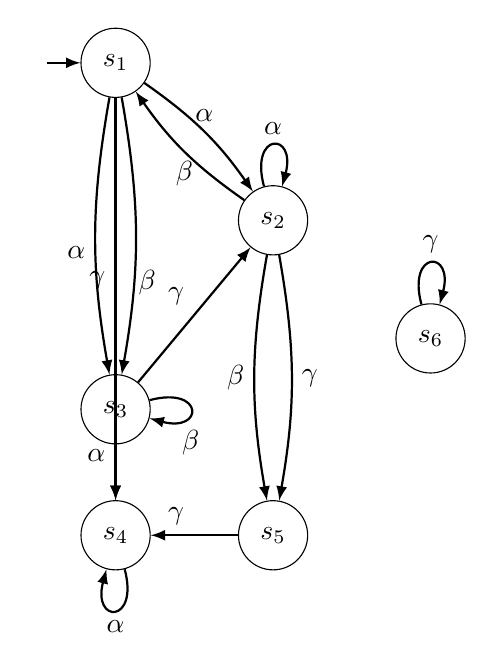
\begin{tikzpicture} [scale=2, every initial by arrow/.style={thick}]
		

		\path
		(\basex,		\basey) 		node[state,init] (s1) 	{$\state_1$} 
		(\basex+2,		\basey+0) 		node[state] (s2) 	{$\state_2$} 
		(\basex+1,		\basey-1.2) 	node[state] (s3) 	{$\state_3$} 
		(\basex,		\basey-2) 		node[state] (s4) 	{$\state_4$} 
		(\basex+2,		\basey-2) 		node[state] (s5) 	{$\state_5$}
		(\basex+3,		\basey-.75) 	node[state] (s6) 	{$\state_6$}
				
		;
		
%		
		\path [bendtrans] 	(s1) 	edge node [midway,above]				{\action} 		(s2);
		\path [bendtrans] 	(s1) 	edge node [near end,above right=-2pt]	{\actionb} 		(s3);
		\path [bendtransr] 	(s1) 	edge node [midway,below left]	{\action} 		(s3);
		\path [trans] 		(s1) 	edge node [midway,above left]	{\actionc} 		(s4);
		\path [bendtrans] 	(s2) 	edge node [midway,below]		{\actionb} 		(s1);
		\path [bendtransr] 	(s2) 	edge node [midway,left]			{\actionb} 		(s5);
		\path [bendtrans] 	(s2) 	edge node [midway,right]		{\actionc} 		(s5);
		\path [trans] 		(s3)	edge node [midway,above left]	{\actionc} 		(s2);
		\path [trans] 		(s3)	edge node [midway,above left]	{\action} 		(s4);
		\path [trans] 		(s5)	edge node [midway,above left]	{\actionc} 		(s4);
		
		\path [trans] 		(s2) 	edge [loop above] node [midway,above] {\action} 	(s2);
		\path [trans] 		(s3) 	edge [loop right] node [midway,below=4pt] {\actionb} 	(s3);
		\path [trans] 		(s4) 	edge [loop below] node [midway,below] {\action} 	(s4);
		\path [trans] 		(s6) 	edge [loop above] node [midway,above] {\actionc} 	(s6);
		
		
		%		midway, at start, near start, very near start, at end, near end, very near end
		
		
	\end{tikzpicture}
\end{document}
	\end{minipage}%
	\begin{minipage}{.5\textwidth}						
		\centering
		\documentclass[tikz,preview]{standalone}
%\usepackage{prelude}

%%%%%%%%%%%%%%%%%%%%%%%%%%%%%%%%%%%% PACKAGES %%%%%%%%%%%%%%%%%%%%%%%%%%%%%%%%%%%%%%%%%%

\usepackage{inputenc,fontenc}
\usepackage[a4paper,margin=3cm]{geometry}
\usepackage[english]{babel}
%\usepackage[german]{babel}
%\usepackage[fixlanguage]{babelbib}


\usepackage{bbold}
\usepackage{amsthm}
\usepackage{amsmath}
\usepackage{amssymb} % doteqdot
\usepackage[dvipsnames]{xcolor}
\usepackage{standalone}
\usepackage{tikz}[mode=buildnew]
\usepackage{cite}
\usepackage{xspace}
\usepackage{relsize}
\usepackage{mathtools} % mathclap
%\usepackage{MnSymbol}
\usepackage{hyperref}
\usepackage{url}
\usepackage{listings} % for code
\usepackage[T1]{fontenc} %<
\hypersetup{
	colorlinks,
	citecolor=black,
	filecolor=black,
	linkcolor=black,
	urlcolor=black
}
\usepackage{pgfplots}
\pgfplotsset{compat=1.18}
%\usepackage{courier} %% Sets font for listing as Courier. But also for url and texttt!
\usepackage{listings, xcolor}
\usepackage{graphicx}
\usepackage{subcaption}

\usetikzlibrary{calc}
%\usepackage{xparse} % \newDocumentCommand for multiple optional arguments
%\usepackage{titlecaps}



%%%%%%%%%%%%%%%%%%%%%%%%%%%%%%%%%%%% THEOREMSTYLES %%%%%%%%%%%%%%%%%%%%%%%%%%%%%%%%%%

\theoremstyle{definition}
\newtheorem{definition}{Definition}[section]
\newtheorem{exmp}{Beispiel}[section]
%\AfterEndEnvironment{definition}{\noindent\ignorespaces}

\theoremstyle{theorem}
\newtheorem{theorem}{Satz}[section]
\newtheorem{proposition}{Proposition}[section]
%\AfterEndEnvironment{theorem}{\noindent\ignorespaces}

\theoremstyle{korollary}
\newtheorem{korollary}{Korollar}[section]
%\AfterEndEnvironment{korollary}{\noindent\ignorespaces}


\tikzset{
	mstate/.style={draw, circle, minimum size=.94cm}, 
	gstate/.style={draw, rectangle, minimum size=.8cm},
	varstate/.style={draw,rectangle, rounded corners, minimum size=1}, 
	trans/.style={draw, ->, thick},
	bendtrans/.style={draw, ->, thick, bend left=10},
	bendtransr/.style={draw, ->, thick, bend right=10},
	init/.style={initial, initial distance=6pt, initial text=},
	every loop/.style={min distance=5pt, looseness=8},
	>=latex
}
\usetikzlibrary{automata,positioning}

%auto shift/.style={auto=right,->,
%	to path={ let \p1=(\tikztostart),\p2=(\tikztotarget),
%		\n1={atan2(\y2-\y1,\x2-\x1)},\n2={\n1+180}
%		in ($(\tikztostart.{\n1})!1mm!270:(\tikztotarget.{\n2})$) -- 
%		($(\tikztotarget.{\n2})!1mm!90:(\tikztostart.{\n1})$) \tikztonodes}},

%%%%%%%%%%%%%%%%%%%%%%%%%%%%%%%%%%% MY MACROS %%%%%%%%%%%%%%%%%%%%%%%%%%%%%%%%%%%%%%%%%
%formatting
\newcommand{\comment}[2]{{\color{#1}#2}}
\newcommand{\redcomment}[1]{{\color{red}#1}}
\newcommand{\purpcomment}[1]{{\color{pink}#1}}
\newcommand{\bluecomment}[1]{{\color{blue}#1}}
\newcommand{\mt}[1]{\ensuremath{{#1}}\xspace}
\newcommand{\mynewcommand}[2]{\newcommand{#1}{\mt{#2}}} %% currently not used becaue of ide highlighting
\newcommand{\arr}{\mt{\to}}

%model checking terms
\newcommand{\mimicrel}{\mt{\mathcal{R}}}
\newcommand{\bisimeq}{\mt{\;\!\sim\;\!}}
\newcommand{\simorder}{\mt{\;\!\preceq\;\!}}
\newcommand{\simequiv}{\mt{\;\!\simeq\;\!}} %command already defined
\newcommand{\relts}{\mt{\;\!\bullet_{_{\tiny{TS}}}\;\!}}
\newcommand{\rel}{\mt{\;\!\bullet\;\!}}

%own names
\newcommand{\nm}[1]{#1\xspace}
\newcommand{\mdpN}{\nm{MDP}}
\newcommand{\mdpsN}{\nm{MDPs}}
\newcommand{\viewN}{\nm{view}}
\newcommand{\viewNC}{\nm{View}}
\newcommand{\viewsN}{\nm{views}}
\newcommand{\viewsNC}{\nm{Views}}
\newcommand{\grpfctsubN}{\nm{detached grouping function}}
\newcommand{\grpfctsubNC}{\nm{detached grouping function}}
\newcommand{\grpfctsubNCC}{\nm{Detached Grouping Function}}
\newcommand{\grpfctN}{\nm{grouping function}}
\newcommand{\grpfctNC}{\nm{Grouping function}}
\newcommand{\grpfctNCC}{\nm{Grouping Function}}
\newcommand{\grpfctsN}{\nm{grouping functions}}
\newcommand{\grpfctsNC}{\nm{Grouping functions}}
\newcommand{\grpfctsNCC}{\nm{Grouping Functions}}
\newcommand{\stmimicN}{\nm{state-mimic}}
\newcommand{\stmimicsN}{\nm{state-mimics}}
\newcommand{\stmimickingN}{\nm{state-mimicking}}
\newcommand{\stmimickedN}{\nm{state-mimicked}}
%\newcommand{\chosenphtypeNCC}{\nm{Transition System}}
%\newcommand{\chgphNC}{\nm{Transition system}}
%\newcommand{\chgphN}{\nm{transition system}}
%\newcommand{\chgphsNCC}{\nm{Transition Systems}}
%\newcommand{\chgphsNC}{\nm{Transition systems}}
%\newcommand{\chgphsN}{\nm{transition systems}}
\newcommand{\chgphNCC}{\nm{MDP}}
\newcommand{\chgphNC}{\nm{MDP}}
\newcommand{\chgphN}{\nm{MDP}}
\newcommand{\achgphN}{\nm{an MDP}}
\newcommand{\chgphsNCC}{\nm{MDPs}}
\newcommand{\chgphsNC}{\nm{MDPs}}
\newcommand{\chgphsN}{\nm{MDPs}}
\newcommand{\parllcompN}{\nm{parallel composition}}
\newcommand{\parllcompNC}{\nm{Parallel composition}}
\newcommand{\parllcompNCC}{\nm{Parallel Composition}}
\newcommand{\parllcompsN}{\nm{parallel compositions}}
\newcommand{\parllcompsNC}{\nm{Parallel compositions}}
\newcommand{\parllcompsNCC}{\nm{Parallel Compositions}}
\newcommand{\sccN}{\nm{SCC}}
\newcommand{\sccsN}{\nm{SCCs}}
\newcommand{\bsccN}{\nm{BSCC}}
\newcommand{\bsccsN}{\nm{BSCCs}}
\newcommand{\jgrapht}{\nm{jGraphtT}}

\newcommand{\outactident}{\nm{OutActionsIdent}}

%names
\newcommand{\iffN}{\nm{if and only if}}
\newcommand{\tsN}{\nm{TS}}

%% outactions identical
\newcommand{\outactidentstrong}{\nm{strong}}
\newcommand{\outactidentweak}{\nm{weak}}

% CORE DEFINITIONS
\newcommand{\grpfct}[1][\viewppty]{\mt{F_{#1}}}
\newcommand{\grpfctsub}[1][\viewppty]{\mt{\tilde{F}_{#1}}}
%\newcommand{\grpfctimg}[1]{\mt{{\grpfct}[{#1}]}}
%\newcommand{\fctimg}[2]{\mt{{#1}[{#2}]}}
\newcommand{\eqrelview}{\mt{R}}
\newcommand{\eqclassv}[1][\state]{\mt{\eqclass{#1}{\eqrelview}}}
\newcommand{\eqclasssetv}[1][\states]{\mt{{#1}/\eqrelview}} %OLD: \bigcup_{\state \in \states} \eqclassv
\newcommand{\viewid}{\mt{\mdp}}
\newcommand{\view}[1][\viewppty]{\mt{\viewid_{#1}}}
\newcommand{\imggrp}{\mt{\arbset}}
\newcommand{\imggrpsub}{\mt{X}}
\newcommand{\viewppty}{\mt{\theta}}
\newcommand{\pll}{\mt{\;\!\pllpure\;\!}}
\newcommand{\pllrev}{\mt{\pllpure^{-1}}}
\newcommand{\pllpure}{\mt{||}}
\newcommand{\compselectset}{\mt{Z}}
\newcommand{\compselectpure}{\mt{\pllpure_\compselectset}}
\newcommand{\compselect}{\mt{\;\pllpure_\compselectset\;}}
\newcommand{\remstates}{\mt{\bigcup_{\state \in \states \setminus \states_1}\{\{\state\}\}}}
\newcommand{\nogroupstates}[1][\states_2]{\mt{\bigcup_{\state \in \states \setminus {#1}}\{\{\state\}\}}}
\newcommand{\remelem}{\mt{\bullet}}
\newcommand{\nogroupset}{\mt{\xi}}
\newcommand{\remset}{\mt{\{\remelem\}}}
\newcommand{\gfctpll}{\mt{\grpfct[\pll]}}
\newcommand{\group}{\mt{\top}}
\newcommand{\imggrpbinview}{\mt{\{\remelem, \notppty\}}}
\newcommand{\viewappset}{\mt{\tilde{\states}}}
\newcommand{\hasppty}{\mt{\top}}
\newcommand{\notppty}{\mt{\bot}}
\newcommand{\disregardelem}{\mt{\Delta}}
\newcommand{\disregardelements}{\mt{{\disregardelem_1, \dots, \disregardelem_n}}}



%\newcommand{\mdp}{def}\mdp
%\newcommand{\mdpdef}



% EXAMPLE VIEWS
\newcommand{\pptyatomicprops}{\mt{\atomicprops}}
\newcommand{\pptyinitstates}{\mt{\initstates}}
\newcommand{\pptyinactsetsize}{\mt{|\inacts(\state)|}}
\newcommand{\pptyhasoutact}{\mt{\exists\outact}}
\newcommand{\pptyminoutact}[2]{\mt{#1\leq#2}}
\newcommand{\pptymaxoutact}[2]{\mt{#2\leq#1}}
\newcommand{\pptyspanoutact}[3]{\mt{#1\leq#2\leq#3}}
\newcommand{\pptyoutactsetsize}{\mt{|\outacts(\state)|}}
\newcommand{\pptyoutactsingle}{\mt{|\outacts(\state)|_1}}
\newcommand{\pptystrongoutactident}{\mt{\outacts(\state)_=}}
\newcommand{\pptyweakoutactident}{\mt{\outacts(\state)_\approx}}
\newcommand{\pptyhasinact}{\mt{\exists\inact}}
\newcommand{\pptymininact}[2]{\mt{#1\leq#2}}
\newcommand{\pptymaxinact}[2]{\mt{#2\leq#1}}
\newcommand{\pptyspaninact}[3]{\mt{#1\leq#2\leq#3}}
\newcommand{\pptyinactsingle}{\mt{|\inacts(\state)|_1}}
\newcommand{\pptystronginactident}{\mt{\inacts(\state)_=}}
\newcommand{\pptyweakinactident}{\mt{\inacts(\state)_\approx}}
\newcommand{\pptyparamvalueseq}{\mt{\var = \varval}}
\newcommand{\pptyparamvaluesneq}{\mt{\var \neq \varval}}
\newcommand{\pptyparamdnf}{\mt{VarDNF}}
\newcommand{\pptyparamcnf}{\mt{VarCNF}}
\newcommand{\pptyparamvalueseqopt}{\mt{\var = \varval}}
\newcommand{\pptyparamvalident}{\mt{Var:\varval}}
\newcommand{\pptydistance}{\mt{\distpath}}
\newcommand{\pptydistancerev}{\mt{\distpathrev}}
\newcommand{\pptydistancebi}{\mt{\distpathbi}}
\newcommand{\pptyhascycle}{\mt{\exists\cycle}}
\newcommand{\pptyexactactcycle}{\mt{\{\cycle_{\action,n}\}}}
\newcommand{\pptycycleset}{\mt{\cup{\{\state\}_\cycle}}}
\newcommand{\pptyexactcycle}{\mt{\{\cycle_n\}}}
\newcommand{\pptyscc}{\mt{scc}}
\newcommand{\pptybscc}{\mt{bscc}}
\newcommand{\pptyprop}{\mt{\redcomment{?}}}
\newcommand{\pptyident}{id}


\newcommand{\gfctatomicprops}{\mt{\grpfct[\pptyatomicprops]}}
\newcommand{\gfctinitstates}{\mt{\grpfct[\pptyinitstates]^\hasppty}}
\newcommand{\gfcthasoutaction}{\mt{\grpfct[\pptyhasoutact]^\hasppty}}
\newcommand{\gfctminoutaction}{\mt{\grpfct[\pptyminoutact{\numoutact}{\outact}]^\hasppty}}
\newcommand{\gfctmaxoutaction}{\mt{\grpfct[\pptymaxoutact{\numoutact}{\outact}]^\hasppty}}
\newcommand{\gfctspanoutaction}{\mt{\grpfct[\pptyspanoutact{\numoutactb}{\outact}{\numoutact}]^\hasppty}}
\newcommand{\gfctoutactsetsize}{\mt{\grpfct[\pptyoutactsetsize]}}
\newcommand{\gfctoutactsingle}{\mt{\grpfct[\pptyoutactsingle]^\notppty}}
\newcommand{\gfctstrongoutactident}{\mt{\grpfct[\pptystrongoutactident]}}
\newcommand{\gfctweakoutactident}{\mt{\grpfct[\pptyweakoutactident]}}
\newcommand{\gfcthasinaction}{\mt{\grpfct[\pptyhasinact]^\hasppty}}
\newcommand{\gfctmininaction}{\mt{\grpfct[\pptymininact{\numinact}{\inact}]^\hasppty}}
\newcommand{\gfctmaxinaction}{\mt{\grpfct[\pptymaxinact{\numinact}{\inact}]^\hasppty}}
\newcommand{\gfctspaninaction}{\mt{\grpfct[\pptyspaninact{\numinactb}{\inact}{\numinact}]^\hasppty}}
\newcommand{\gfctinactsetsize}{\mt{\grpfct[\pptyinactsetsize]}}
\newcommand{\gfctinactsingle}{\mt{\grpfct[\pptyinactsingle]^\notppty}}
\newcommand{\gfctstronginactident}{\mt{\grpfct[\pptystronginactident]}}
\newcommand{\gfctweakinactident}{\mt{\grpfct[\pptyweakinactident]}}
\newcommand{\gfctparamvalueseq}{\mt{\grpfct[\pptyparamvalueseq]^\hasppty}}
\newcommand{\gfctparamvaluesneq}{\mt{\grpfct[\pptyparamvaluesneq]^\hasppty}}
\newcommand{\gfctparamdnf}{\mt{\grpfct[\pptyparamdnf]^\hasppty}}
\newcommand{\gfctparamcnf}{\mt{\grpfct[\pptyparamcnf]^\hasppty}}
\newcommand{\gfctparamvalueseqopt}{\mt{\pptyparamvalueseqopt}}
\newcommand{\gfctparamvalident}{\mt{\grpfct[\pptyparamvalident]}}
\newcommand{\gfctdistance}{\mt{\grpfct[\pptydistance]}}
\newcommand{\gfctdistancerev}{\mt{\grpfct[\pptydistancerev]}}
\newcommand{\gfctdistancebi}{\mt{\grpfct[\pptydistancebi]}}
\newcommand{\gfcthascycle}{\mt{\grpfct[\pptyhascycle]}}
\newcommand{\gfctexactcycle}{\mt{\grpfct[\pptyexactcycle]}}
\newcommand{\gfctcycleset}{\mt{\grpfct[\pptycycleset]}}
\newcommand{\gfctexactactcycle}{\mt{\grpfct[\pptyexactactcycle]}}
\newcommand{\gfctscc}{\mt{\grpfct[\pptyscc]}}
\newcommand{\gfctbscc}{\mt{\grpfct[\pptybscc]}}
\newcommand{\gfctprop}{\mt{\grpfct[\pptyprop]}}
\newcommand{\gfctident}{\mt{\grpfct[\pptyident]}}

\newcommand{\gfctsubatomicprops}{\mt{\grpfctsub[\pptyatomicprops]}}
\newcommand{\gfctsubinitstates}{\mt{\grpfctsub[\pptyinitstates]^\hasppty}}
\newcommand{\gfctsubhasoutaction}{\mt{\grpfctsub[\pptyhasoutact]^\hasppty}}
\newcommand{\gfctsubminoutaction}{\mt{\grpfctsub[\pptyminoutact{\numoutact}{\outact}]^\hasppty}}
\newcommand{\gfctsubmaxoutaction}{\mt{\grpfctsub[\pptymaxoutact{\numoutact}{\outact}]^\hasppty}}
\newcommand{\gfctsubspanoutaction}{\mt{\grpfctsub[\pptyspanoutact{\numoutactb}{\outact}{\numoutact}]^\hasppty}}
\newcommand{\gfctsuboutactsetsize}{\mt{\grpfctsub[\pptyoutactsetsize]}}
\newcommand{\gfctsuboutactsingle}{\mt{\grpfctsub[\pptyoutactsingle]^\notppty}}
\newcommand{\gfctsubstrongoutactident}{\mt{\grpfctsub[\pptystrongoutactident]^\hasppty}}
\newcommand{\gfctsubweakoutactident}{\mt{\grpfctsub[\pptyweakoutactident]^\hasppty}}
\newcommand{\gfctsubhasinaction}{\mt{\grpfctsub[\pptyhasinact]}}
\newcommand{\gfctsubmininaction}{\mt{\grpfctsub[\pptymininact{\numinact}{\inact}]}}
\newcommand{\gfctsubmaxinaction}{\mt{\grpfctsub[\pptymaxinact{\numinact}{\inact}]}}
\newcommand{\gfctsubspaninaction}{\mt{\grpfctsub[\pptyspaninact{\numinactb}{\inact}{\numinact}]}}
\newcommand{\gfctsubinactsetsize}{\mt{\grpfctsub[\pptyinactsetsize]^\hasppty}}
\newcommand{\gfctsubinactsingle}{\mt{\grpfctsub[\pptyinactsingle]^\notppty}}
\newcommand{\gfctsubstronginactident}{\mt{\grpfctsub[\pptystronginactident]}}
\newcommand{\gfctsubweakinactident}{\mt{\grpfctsub[\pptyweakinactident]}}
\newcommand{\gfctsubparamvalueseq}{\mt{\grpfctsub[\pptyparamvalueseq]^\hasppty}}
\newcommand{\gfctsubparamvaluesneq}{\mt{\grpfctsub[\pptyparamvaluesneq]^\hasppty}}
\newcommand{\gfctsubparamdnf}{\mt{\grpfctsub[\pptyparamdnf]^\hasppty}}
\newcommand{\gfctsubparamcnf}{\mt{\grpfctsub[\pptyparamcnf]^\hasppty}}
\newcommand{\gfctsubparamvalueseqopt}{\mt{\pptyparamvalueseqopt}}
\newcommand{\gfctsubparamvalident}{\mt{\grpfctsub[\pptyparamvalident]}}
\newcommand{\gfctsubdistance}{\mt{\grpfctsub[\pptydistance]}}
\newcommand{\gfctsubdistancerev}{\mt{\grpfctsub[\pptydistancerev]}}
\newcommand{\gfctsubdistancebi}{\mt{\grpfctsub[\pptydistancebi]}}
\newcommand{\gfctsubhascycle}{\mt{\grpfctsub[\pptyhascycle]^\hasppty}}
\newcommand{\gfctsubexactcycle}{\mt{\grpfctsub[\pptyexactcycle]}}
\newcommand{\gfctsubcycleset}{\mt{\grpfctsub[\pptycycleset]}}
\newcommand{\gfctsubexactactcycle}{\mt{\grpfctsub[\pptyexactactcycle]}}
\newcommand{\gfctsubscc}{\mt{\grpfctsub[\pptyscc]}}
\newcommand{\gfctsubbscc}{\mt{\grpfctsub[\pptybscc]}}
\newcommand{\gfctsubprop}{\mt{\grpfctsub[\pptyprop]}}
\newcommand{\gfctsubident}{\mt{\grpfctsub[\pptyident]}}


\newcommand{\viewatomicprops}{\mt{\view[\pptyatomicprops]}}
\newcommand{\viewinitstates}{\mt{\view[\pptyinitstates]^\hasppty}}
\newcommand{\viewhasoutaction}{\mt{\view[\pptyhasoutact]^\hasppty}}
\newcommand{\viewminoutaction}{\mt{\view[\pptyminoutact{\numoutact}{\outact}]^\hasppty}}
\newcommand{\viewmaxoutaction}{\mt{\view[\pptymaxoutact{\numoutact}{\outact}]^\hasppty}}
\newcommand{\viewspanoutaction}{\mt{\view[\pptyspanoutact{\numoutactb}{\outact}{\numoutact}]^\hasppty}}
\newcommand{\viewoutactsetsize}{\mt{\view[\pptyoutactsetsize]}}
\newcommand{\viewoutactsingle}{\mt{\view[\pptyoutactsingle]^\notppty}}
\newcommand{\viewstrongoutactident}{\mt{\view[\pptystrongoutactident]}}
\newcommand{\viewweakoutactident}{\mt{\view[\pptyweakoutactident]}}
\newcommand{\viewhasinaction}{\mt{\view[\pptyhasinact]^\hasppty}}
\newcommand{\viewmininaction}{\mt{\view[\pptymininact{\numinact}{\inact}]^\hasppty}}
\newcommand{\viewmaxinaction}{\mt{\view[\pptymaxinact{\numinact}{\inact}]^\hasppty}}
\newcommand{\viewspaninaction}{\mt{\view[\pptyspaninact{\numinactb}{\inact}{\numinact}]^\hasppty}}
\newcommand{\viewinactsetsize}{\mt{\view[\pptyinactsetsize]}}
\newcommand{\viewinactsingle}{\mt{\view[\pptyinactsingle]^\notppty}}
\newcommand{\viewstronginactident}{\mt{\view[\pptystronginactident]}}
\newcommand{\viewweakinactident}{\mt{\view[\pptyweakinactident]}}
\newcommand{\viewparamvalueseq}{\mt{\view[\pptyparamvalueseq]}}
\newcommand{\viewparamvaluesneq}{\mt{\view[\pptyparamvaluesneq]}}
\newcommand{\viewparamdnf}{\mt{\view[\pptyparamdnf]^\hasppty}}
\newcommand{\viewparamcnf}{\mt{\view[\pptyparamcnf]^\hasppty}}
\newcommand{\viewparamvalueseqopt}{\mt{\pptyparamvalueseqopt}}
\newcommand{\viewparamvalident}{\mt{\view[\pptyparamvalident]}}
\newcommand{\viewdistance}{\mt{\view[\pptydistance]}}
\newcommand{\viewdistancerev}{\mt{\view[\pptydistancerev]}}
\newcommand{\viewdistancebi}{\mt{\view[\pptydistancebi]}}
\newcommand{\viewhascycle}{\mt{\view[\pptyhascycle]}}
\newcommand{\viewexactcycle}{\mt{\view[\pptyexactcycle]}}
\newcommand{\viewcycleset}{\mt{\view[\pptycycleset]}}
\newcommand{\viewexactactcycle}{\mt{\view[\pptyexactactcycle]}}
\newcommand{\viewscc}{\mt{\view[\pptyscc]}}
\newcommand{\viewbscc}{\mt{\view[\pptybscc]}}
\newcommand{\viewprop}{\mt{\view[\pptyprop]}}
\newcommand{\viewident}{\mt{\view[\pptyident]}}

%\newcommand{\viewatomicprops}{\mt{\view[\atomicprops]}}
%\newcommand{\viewinitstates}{\mt{\view[\initstates]}}
%\newcommand{\viewhasoutaction}{\mt{\view[\pptyhasoutact]}}
%\newcommand{\viewminoutaction}{\mt{\view[\pptyminoutact{\numoutact}{\outact}]}}
%\newcommand{\viewmaxoutaction}{\mt{\view[\pptymaxoutact{\numoutact}{\outact}]}}
%\newcommand{\viewspanoutaction}{\mt{\view[\pptyspanoutact{\numoutactb}{\outact}{\numoutact}]}}
%\newcommand{\viewoutactsetsize}{\mt{\view[\pptyoutactsetsize]}}
%\newcommand{\viewoutactsingle}{\mt{\view[\pptyoutactsingle]}}
%\newcommand{\viewstrongoutactident}{\mt{\view[\outacts(\state)_=]}}
%\newcommand{\viewweakoutactident}{\mt{\view[\outacts(\state)_\approx]}}
%\newcommand{\viewhasinaction}{\mt{\view[\pptyhasinact]}}
%\newcommand{\viewmininaction}{\mt{\view[\pptymininact{\numinact}{\inact}]}}
%\newcommand{\viewmaxinaction}{\mt{\view[\pptymaxinact{\numinact}{\inact}]}}
%\newcommand{\viewspaninaction}{\mt{\view[\pptyspaninact{\numinactb}{\inact}{\numinact}]}}
%\newcommand{\viewinactsetsize}{\mt{\view[\pptyinactsetsize]}}
%\newcommand{\viewinactsingle}{\mt{\view[\pptyinactsingle]}}
%\newcommand{\viewstronginactident}{\mt{\view[\inacts(\state)_=]}}
%\newcommand{\viewweakinactident}{\mt{\view[\inacts(\state)_\approx]}}
%\newcommand{\viewparamvalueseq}{\mt{\view[\var = \varval]}}
%\newcommand{\viewparamvaluesneq}{\mt{\view[\var \neq \varval]}}
%\newcommand{\viewparamdnf}{\mt{\view[VarDNF]}}
%\newcommand{\viewparamcnf}{\mt{\view[VarCNF]}}
%\newcommand{\viewparamvalident}{\mt{\view[\pptyparamvalident]}}
%\newcommand{\viewdistance}{\mt{\view[\pptydistance]}}
%\newcommand{\viewhascycle}{\mt{\view[\exists\cycle]}}
%\newcommand{\viewexactcycle}{\mt{\view[\pptyexactcycle]}}
%\newcommand{\viewcycleset}{\mt{\view[\pptycycleset]}}
%\newcommand{\viewexactactcycle}{\mt{\view[\pptyexactactcycle]}}
%\newcommand{\viewscc}{\mt{\view[scc]}}
%\newcommand{\viewbscc}{\mt{\view[bscc]}}

%actions
\newcommand{\numoutact}{\mt{n}}
\newcommand{\numoutactb}{\mt{m}}
\newcommand{\numinact}{\mt{n}}
\newcommand{\numinactb}{\mt{m}}

\newcommand{\predmaxoutact}[1][\numoutact]{\mt{Q_{\outact\leq#1}(\state,\state_1, \dots, \state_{#1+1})}}
\newcommand{\predminoutact}[1][\numoutact]{\mt{Q_{#1\leq\outact}(\state,\state_1, \dots, \state_{#1})}}
\newcommand{\formoutact}[1][\state]{\mt{C_{#1,\outact}}}
\newcommand{\predmaxinact}[1][\numinact]{\mt{Q_{\inact\leq#1}(\state,\state_1, \dots, \state_{#1+1})}}
\newcommand{\predmininact}[1][\numinact]{\mt{Q_{#1\leq\inact}(\state,\state_1, \dots, \state_{#1})}}

\newcommand{\outact}[1][\action]{\mt{\overrightarrow{#1}}}
\newcommand{\outacts}{\mt{\overrightarrow{\actions}}}
\newcommand{\inact}{\mt{\overleftarrow{\action}}}
\newcommand{\inacts}[1][\action]{\mt{\overleftarrow{#1}}}

%%Parameters
\newcommand{\vars}[1][\mdp]{\mt{V\!ar_{#1}}}
\newcommand{\var}{\mt{x}}
\newcommand{\varstate}[1][]{\mt{\var_{\state#1}}}
\newcommand{\varval}{\mt{a}}
\newcommand{\vareval}[1][\mdp]{\mt{V\!arEval_{#1}}}
\newcommand{\varevalimg}[1][\mdp]{\mt{\vareval[#1][\states,\vars]}}
\newcommand{\varevalimgset}{\mt{\arbset}}
\newcommand{\someparam}{\mt{\tilde{x}}}
\newcommand{\eqorneq}{\mt{\;\doteqdot\;}}
\newcommand{\varstyle}[2]{\mt{\langle#1,#2\rangle}}




%\makeatletter
%\newcommand{\overleftrightsmallarrow}{\mathpalette{\overarrowsmall@\leftrightarrowfill@}}
%\newcommand{\overrightsmallarrow}{\mathpalette{\overarrowsmall@\rightarrowfill@}}
%\newcommand{\overleftsmallarrow}{\mathpalette{\overarrowsmall@\leftarrowfill@}}
%\newcommand{\overarrowsmall@}[3]{%
%	\vbox{%
%		\ialign{%
%			##\crcr
%			#1{\smaller@style{#2}}\crcr
%			\noalign{\nointerlineskip}%
%			$\m@th\hfil#2#3\hfil$\crcr
%		}%
%	}%
%}
%\def\smaller@style#1{%
%	\ifx#1\displaystyle\scriptstyle\else
%	\ifx#1\textstyle\scriptstyle\else
%	\scriptscriptstyle
%	\fi
%	\fi
%}
%\makeatother
%\newcommand{\te}[1]{\overleftrightsmallarrow{#1}}

% Distance
\newcommand{\fctdist}{\mt{distance}}
\newcommand{\fctdistdefault}{\mt{\fctdist(\chgph, \smstates, \grandist)}}
\newcommand{\distval}{\mt{d}}
\newcommand{\grandist}{\mt{n}}
\let\path\oldpath
\newcommand{\path}{\mt{P}}
\newcommand{\pathbi}{\mt{\bar{\path}}}
\newcommand{\pathsecfull}{\mt{(\state_0, \action_0, \state_1, \action_1, \dots, \action_{n}, \state_{n+1})}}
\newcommand{\lenpath}{\mt{len}}
\newcommand{\pfirst}{\mt{first}}
\newcommand{\plast}{\mt{last}}
\newcommand{\pathset}{\mt{\path_\chgph}}
\newcommand{\pathbiset}{\mt{\pathbi_\chgph}}
\newcommand{\distpath}{\mt{\overrightarrow{dist}}}
\newcommand{\distpathrev}{\mt{\overleftarrow{dist}}}
\newcommand{\distpathbi}{\mt{\overline{dist}}}
%Cycles
\newcommand{\cyclesecfull}{\mt{(\state_0, \action_0, \state_1, \action_1, \dots, \action_{n-1}, \state_0)}}
\newcommand{\fctfindcycles}{\mt{findCycles}}
\newcommand{\cycle}{\mt{C}}
\newcommand{\cycleset}{\mt{\cycle_{\mdp, n}}}
\newcommand{\lencycle}{\mt{len}}
% strongly connected components
\newcommand{\scc}{\mt{T}}
\newcommand{\setscc}{\mt{SCC_{\chgph,n}}}
\newcommand{\setbscc}{\mt{BSCC_{\chgph,n}}}

% properties
\newcommand{\propfct}{\mt{f}}

% all Systems
\newcommand{\chgph}{\mt{\mdp}}
\newcommand{\chgphtuple}{\mt{\mdptuple}}
\newcommand{\chgphtupledist}{\mt{\mdptupledist}}

\newcommand{\states}{\mt{S}}
\newcommand{\actions}{\mt{Act}}
\newcommand{\atomicprops}{\mt{AP}}
\newcommand{\labelingfct}{\mt{L}}
\newcommand{\init}{\mt{\initdistrib}} % use MDP % refers to the underlying set
\newcommand{\trans}{\mt{\probtfunc}} % use MDP % refers to the underlying set
\newcommand{\smstates}{\mt{\tilde{\states}}}


\newcommand{\state}{\mt{s}}
\newcommand{\action}{\mt{\alpha}}
\newcommand{\actionb}{\mt{\beta}}
\newcommand{\actionc}{\mt{\gamma}}
\newcommand{\smstate}{\mt{\tilde{\state}}}



% transition sysstems
\newcommand{\ts}{\mt{TS}}
\newcommand{\transitionrel}{\mt{\longrightarrow}}
\newcommand{\initstates}{\mt{I}}
\newcommand{\transitionsystem}{\mt
	{(\states, \actions, \transitionrel, \initstates, \atomicprops, \labelingfct)}
}
\newcommand{\tstupledist}{\mt{(\states', \actions',\transitionrel', \initstates', \labelingfct')}}


%Markov chains and MDP
\newcommand{\mdp}{\mt{\autm}}
\newcommand{\mdptuple}{\mt{(\states, \actions, \probtfunc, \initdistrib, \atomicprops, \labelingfct)}}
\newcommand{\mdptupledist}{\mt{(\states', \actions', \probtfunc', \initdistrib', \atomicprops', \labelingfct')}}
\newcommand{\autm}{\mt{\mathcal{M}}}
\newcommand{\probtfunc}{\mt{\textbf{P}}}
\newcommand{\initdistrib}{\mt{\iota_{init}}}


%maths
\newcommand{\powerset}[1]{\mt{\mathcal{P}(#1)}}
\newcommand{\eqclass}[2]{\mt{[#1]_{#2}}}%{\mt{#1 / #2}}
\newcommand{\impr}{\mt{\hspace{3mm}\Rightarrow\hspace{2mm}}}
\newcommand{\impl}{\mt{\hspace{3mm}\Leftarrow\hspace{2mm}}}
\newcommand{\natnums}{\mt{\mathbb{N}}} 
\newcommand{\realnums}{\mt{\mathbb{R}}}
\newcommand{\intmodn}[1][n]{\mt{\mathbb{Z}_{#1}}}
\newcommand{\arbset}{\mt{M}}
\newcommand{\bigsum}[2][]{\mt{\mathlarger{\sum}_{#2}^{#1}}}
\newcommand{\bbigsum}[2][]{\mt{\mathlarger{\mathlarger{\sum}}_{#2}^{#1}}}
\newcommand{\invimage}[2]{#1^{\mt{-1}(#2)}}
\newcommand{\img}{\mt{Img}}
\newcommand{\cond}{\mt{\,|\,}}

%tickz
%% \definecolor{darkred}{RGB}{196, 42, 42}

%implementation
\newcommand{\pmcvis}{\nm{PMC-Vis}}





\begin{document}
	\newcommand{\basex}{0}
	\newcommand{\basey}{0}
	\newcommand{\createstate}[3]{\node[draw, circle, minimum size=1cm] (#1) at (#2) {#3}}
	
	
	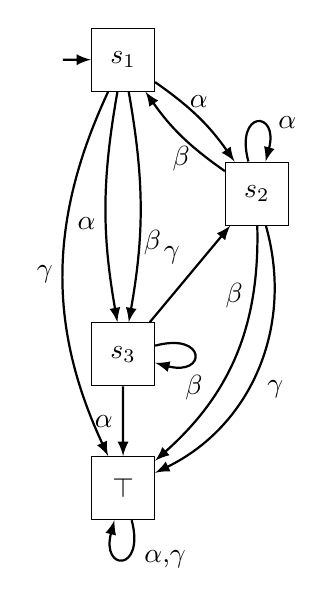
\begin{tikzpicture} [scale=1.7, every initial by arrow/.style={thick}]
		
		
		\path
		(\basex,		\basey) 		node[gstate,init] (s1) 	{$\state_1$} 
		(\basex+2,		\basey+0) 		node[gstate] (s2) 	{$\state_2$} 
		(\basex+1,		\basey-1.2) 	node[gstate] (s3) 	{$\state_3$} 
		(\basex+1,		\basey-2.2) 		node[gstate] (stop) 	{$\hasppty$} 
		
		
		;
		
		%		
		\path [bendtrans] 	(s1) 	edge node [midway,above]				{\action} 		(s2);
		\path [bendtrans] 	(s1) 	edge node [near end,above right=-2pt]	{\actionb} 		(s3);
		\path [bendtransr] 	(s1) 	edge node [midway,below left]	{\action} 		(s3);
		\path [trans,bend right=25] 		(s1) 	edge node [midway,left]	{\actionc} 		(stop);
		\path [bendtrans] 	(s2) 	edge node [midway,below]		{\actionb} 		(s1);
		\path [trans, bend left=25] 	(s2) 	edge node [near start,left]			{\actionb} 		(stop);
		\path [trans,bend left=40] 	(s2) 	edge node [midway,below right]		{\actionc} 		(stop);
		\path [trans] 		(s3)	edge node [midway,above left]	{\actionc} 		(s2);
		\path [trans] 		(s3)	edge node [midway,left]	{\action} 		(stop);

		
		\path [trans] 		(s2) 	edge [loop above] node [midway,right=4pt] {\action} 	(s2);
		\path [trans] 		(s3) 	edge [loop right] node [midway,below=4pt] {\actionb} 	(s3);
		\path [trans] 		(stop) 	edge [loop below] node [midway,right=4pt] {\action,\actionc} 	(stop);		
		
		
		%		midway, at start, near start, very near start, at end, near end, very near end
		
		
	\end{tikzpicture}
\end{document}
	\end{minipage}	
	\caption{Simplified representations of \mdp (left) and the \viewN \viewoutactsetsize on it (right)}	
	\label{fig:outActSingle}  	
\end{figure}

\subsubsection{Ingoing Actions}
Analogously to Outgoing Actions views of utilizing ingoing actions are feasable. Since there is no difference apart from the definitions itself, we only provide the definitions.

\begin{definition}
	Let $\chgph = \chgphtuple$ be \achgphN and $\action \in \actions$. The view \viewhasinaction is defined by its \grpfctN $\gfcthasinaction : \states \to \imggrp$ with 
	
	\[
	\state \mapsto
	\begin{cases}
			\group,				& \text{if } \exists \state' \in \states: (\state', \action, \state) \in \trans \\
			\remelem,          	& \text{otherwise}
		\end{cases}
	\]
	
	and $\imggrp := \imggrpbinview$.	
	\label{def:mininaction}
\end{definition}	


\begin{definition}
	Let $\chgph = \chgphtuple$ be \achgphN and $\action \in \actions$. The view \viewmininaction is defined by its \grpfctN $\gfctmininaction : \states \to \arbset$ with
	
	\[
	\state \mapsto
	\begin{cases}
			\group,				& \text{if } \exists \state_1, \dots, \state_\numinact \in \states:  \predmininact\\
			\remelem,          	& \text{otherwise}
		\end{cases}
	\]
	
	where $\imggrp := \imggrpbinview$,
%	 $\numinact \in \natnums$ 
	 is the minimum amount of times a transition with action \action has to be ingoing in order to be grouped with the other states and
	\[
	\predmininact := ((\state_1, \action, \state), \dots, (\state_\numinact, \action, \state) \in \trans) \land |\{\state_1, \dots, \state_\numinact\}| = \numinact
	\]
	is a first order logic predicate.
	\label{def:viewmaxinaction}
\end{definition}

\begin{definition}
	Let $\chgph = \chgphtuple$ be \achgphN and $\action \in \actions$. The view \viewmaxinaction is defined by its \grpfctN $\gfctmaxinaction : \states \to \arbset$ with
	
	\[
	\state \mapsto
	\begin{cases}
			\group,				& \text{if } \forall \state_1, \dots, \state_{\numinact+1} \in \states: \predmaxinact \\
			\remelem,          	& \text{otherwise}
		\end{cases}
	\]
	
	where $\imggrp := \imggrpbinview$
%	$\numinact \in \natnums$ 
	 is the maximal number of times a transition with action \action may be ingoing and 
	\[
	\predmaxinact := ((\state_1, \action, \state), \dots, (\state_{\numinact+1}, \action, \state) \in \trans) \implies \bigvee_{\mathclap{\substack{i,j \in \{1,\dots, \numinact+1\} \\ i < j}}} \state_i = \state_j
	\]
	is a first order logic predicate.
\end{definition}

\begin{definition}
	Let $\chgph = \chgphtuple$ be \achgphN and $\action \in \actions$. The view 
	\viewspaninaction is defined by its \grpfctN $\gfctspaninaction : \states \to \arbset$ with
	
	\[
	\state \mapsto
	\begin{cases}
			\group,				& \text{if } \exists \state_1, \dots, \state_\numinactb \in \states: \predmininact[\numinactb] \\ &\text{and } \forall \state_1, \dots, \state_{\numinact+1} \in \states: \predmaxinact \\
			\remelem,          	& \text{otherwise}
		\end{cases}
	\]
	
	where $\imggrp := \imggrpbinview$
%	\actions \cup \remset$ 
	and $\numinactb, \numinact \in \natnums$ are the minimal and maximal number of transitions with action \action in order for state to be grouped. The predicates \predmininact and \predmaxinact are the predicates from Definition \ref{def:mininaction} and Definition \ref{def:viewmaxinaction} respectively.
\end{definition}

\begin{definition}
	Let $\chgph = \chgphtuple$ be \achgphN and $\action \in \actions$. The \viewN \viewstronginactident is defined by its \grpfctN $\gfctstronginactident : \states \to \imggrp$ with
	\[
	\state \mapsto	
	\{(\action, \numinact) \mid \action \in \actions, \numinact \text{ is the number of times that \action is ingoing from } \state\}
	\]
	and $\imggrp := (\actions \times \natnums_0) \cup \remset$.
\end{definition}

\begin{definition}
	Let $\chgph = \chgphtuple$ be \achgphN and $\action \in \actions$. The \viewN \viewweakinactident is defined by its \grpfctN $\gfctweakinactident : \states \to \imggrp$ with
	\[
	\state \mapsto \{\action \in \actions \mid \exists \state' \in \states : (\state', \action, \state) \in \trans\} 	
	\]
	and $\imggrp := \actions\cup \remset$.
\end{definition}

\begin{definition}
	Let $\chgph = \chgphtuple$ be \achgphN and $\action \in \actions$. The \viewN \viewinactsetsize is defined by its \grpfctN $\gfctinactsetsize : \states \to \imggrp$ with
	\[
	\state \mapsto |\{\action \in \actions \mid \exists \state' \in \states : (\state', \action, \state) \in \trans\}|
	\]
	and $\imggrp := \natnums \cup \remset$.
\end{definition}

\subsubsection{Variables}
The concept of variables is not part of the definitions of neither \tsN, MCs or \mdpsN even though, it is of great importance in practice. We will introduce and discuss this concept before utilizing it for \viewsN.

Since states describe some information about a system at a certain moment of its behavior the information carried is usually not atomic but rather consists of several pieces. For instance when considering a computer program at a given moment during execution all its currently available variables will have some value, the stack will have a certain structure and the program counter points to a specific instruction. Systems in general at a certain moment of their behavior have several properties that in total pose the current state of the system. That is in practice each state is actually derived from a possible variable assertion. Choosing the respective variable assertion as state representation would result in rather complex state objects. Therefore the values of the variables are usually stored in a separate data structure and a simple identifier like an integer represents the actual state. When formalizing this in practice used approach several options com into consideration. Available \mdpN components like atomic propositions or the set of states could be used to contain this information. There could be a subset of atomic propositions that declares that a certain variable has a certain value. There had to be taken care that for each variable in each state there is only one atomic proposition declaring its value. The set of states could be used in the sense that the states itself are complex objects containing the information. Both of these options are rather tedious but possible. A third option is to define a set of variables and an evaluation function that are induced by the \mdpN.
%Firstly there is the option of declaring the states as complex objects that contain this information. This would be possible because the set of states is not further specified. Accessing this information stored within a state would be rather tedious because there is no already existing entity to properly accomplishing the access. Hence this option was not further explored. The second option is to require that all possible assertions of all variables are included in the atomic propositions. The labeling function would then assert exactly one atomic proposition for each variable for each state, that specifies what the current value of that variable is. Although this would be possible, for simplicity we chose that variables and its values are provided in addition to the \mdpN. Obviously they are to be understood as derived and therefore dependent on the  system, that the \mdpN has been derived from. By no means the set of variables and its evaluation are arbitrary.


%Variables are used to represent states (in more detail). 
%
%For example an \mdpN could be used to model a computer program with human interaction. Every state of the MDP refers an overall state of the program during execution time. In this state of the program, its variables will have specific values. We may want to retain the information about the variable's values of the program instead of only assigning a state $\state \in \states$ that refers to the state of the program. Variables and its current values are not only relevant to computer programs but also other systems. Many of those other systems rely on some kind of global state during execution, which can be expressed with variables and values assigned to them. Since there exists no explicit component to retain this information the notion of variables is used to store it.
%
%\redcomment{OLD: Since transitions systems MCs and MDPs in practice are used to model, analyze and check real world systems it is very practical to not only name states but also describe the properties of the state in more detail. For a basic notion variables are to be imagined as a set of variables that may have different values in different states thereby describing the characteristics of the state more thoroughly. \purpcomment{ADDED TO OLD: In practice most often they arise naturally for example as variables of a computer program that is to be modeled with an \mdpN.}} 
%
%Because of the vast importance in practical applications we will consider some \viewsN that utilize them. To do so and being able to describe them formally we define and formalize the notion of variables by considering them as a subset of the atomic propositions \atomicprops that is assigned a value by a function.

\begin{definition}
	Let $\mdp$ be an \mdpN. The set $\vars$ is called \emph{variables} (of \mdp). It contains all variables induced by \mdp.
\end{definition}

\begin{definition}
	Let $\mdp = \mdptuple$ be an \mdpN and \varevalimgset be an arbitrary set. The by im induced function $\vareval : \states \times \vars \to \varevalimgset$ is called \emph{variable evaluation function}.
\end{definition} 

Most of the time we will use \vareval to refer to the variable evaluation function. When we speak about the value of a variable in a state we refer to the image of $\vareval$ for that state and variable. The set \varevalimgset is arbitrary so that arbitrary values can be assigned to a variable. Speaking in terms of computer science and programming this loosens as an example the restriction of only being able to assign numbers and no booleans.

The most apparent idea for a \viewN utilizing variables is to group states that meet some requirement regarding the values of the variables.


\redcomment{state has variable not here uptil now because probably not used}

\begin{definition}
	Let $\chgph = \chgphtuple$ be \achgphN, $\var \in \vars$ and $\varval \in \varevalimg$. The view \viewparamvalueseq is defined by its \grpfctN $\gfctparamvalueseq : \states \to \imggrp$ with
	\[
	\state \mapsto
	\begin{cases}
			\group, &\text{if } \vareval(\state, \var) = \varval\\
			\remelem, &\text{otherwise}
		\end{cases}
	\]
	where $\imggrp := \imggrpbinview$.
\end{definition}

The view \viewparamvalueseq groups states that share the same value for a given variable. For $\state_1, \state_2$ it is $\gfctparamvalueseq(\state_1) = \gfctparamvalueseq(\state_2)$ \iffN $\vareval(\state_1, \var) = \vareval(\state_2, \var)$ or $\state_1 = \state_2$. The obtained equivalence classes are
\begin{align*}
	\eqclassv &= \{\state \in \states \mid \vareval(\state, \var) = \varval\} \\
	\eqclassv &= \{\state \in \states \mid \gfctparamvalueseq(\state) = \state\} = \{\state\}
\end{align*}

The set of states $\states'$ of \viewparamvalueseq is the union of the equivalence classes of \eqrelview. It is $\states' = \bigcup_{\state \in \states} \eqclassv =: \states_1 \cup \states_2$ where

\begin{align*}
	\states_1 &:= \{\state \in \states \mid \gfctparamvalueseq(\state) = \varval\} \\
	&\hspace{1.15mm}= \{\state \in \states  \mid \vareval(\state, \var) = \varval\} \text{ and} \\
	\states_2 &:= \remstates.
\end{align*}

\begin{figure}[h]
	\begin{minipage}{.6\textwidth}
		%		\hspace{5mm}		
		\documentclass[tikz]{standalone}
%\usepackage{prelude}

%%%%%%%%%%%%%%%%%%%%%%%%%%%%%%%%%%%% PACKAGES %%%%%%%%%%%%%%%%%%%%%%%%%%%%%%%%%%%%%%%%%%

\usepackage{inputenc,fontenc}
\usepackage[a4paper,margin=3cm]{geometry}
\usepackage[english]{babel}
%\usepackage[german]{babel}
%\usepackage[fixlanguage]{babelbib}


\usepackage{bbold}
\usepackage{amsthm}
\usepackage{amsmath}
\usepackage{amssymb} % doteqdot
\usepackage[dvipsnames]{xcolor}
\usepackage{standalone}
\usepackage{tikz}[mode=buildnew]
\usepackage{cite}
\usepackage{xspace}
\usepackage{relsize}
\usepackage{mathtools} % mathclap
%\usepackage{MnSymbol}
\usepackage{hyperref}
\usepackage{url}
\usepackage{listings} % for code
\usepackage[T1]{fontenc} %<
\hypersetup{
	colorlinks,
	citecolor=black,
	filecolor=black,
	linkcolor=black,
	urlcolor=black
}
\usepackage{pgfplots}
\pgfplotsset{compat=1.18}
%\usepackage{courier} %% Sets font for listing as Courier. But also for url and texttt!
\usepackage{listings, xcolor}
\usepackage{graphicx}
\usepackage{subcaption}

\usetikzlibrary{calc}
%\usepackage{xparse} % \newDocumentCommand for multiple optional arguments
%\usepackage{titlecaps}



%%%%%%%%%%%%%%%%%%%%%%%%%%%%%%%%%%%% THEOREMSTYLES %%%%%%%%%%%%%%%%%%%%%%%%%%%%%%%%%%

\theoremstyle{definition}
\newtheorem{definition}{Definition}[section]
\newtheorem{exmp}{Beispiel}[section]
%\AfterEndEnvironment{definition}{\noindent\ignorespaces}

\theoremstyle{theorem}
\newtheorem{theorem}{Satz}[section]
\newtheorem{proposition}{Proposition}[section]
%\AfterEndEnvironment{theorem}{\noindent\ignorespaces}

\theoremstyle{korollary}
\newtheorem{korollary}{Korollar}[section]
%\AfterEndEnvironment{korollary}{\noindent\ignorespaces}


\tikzset{
	mstate/.style={draw, circle, minimum size=.94cm}, 
	gstate/.style={draw, rectangle, minimum size=.8cm},
	varstate/.style={draw,rectangle, rounded corners, minimum size=1}, 
	trans/.style={draw, ->, thick},
	bendtrans/.style={draw, ->, thick, bend left=10},
	bendtransr/.style={draw, ->, thick, bend right=10},
	init/.style={initial, initial distance=6pt, initial text=},
	every loop/.style={min distance=5pt, looseness=8},
	>=latex
}
\usetikzlibrary{automata,positioning}

%auto shift/.style={auto=right,->,
%	to path={ let \p1=(\tikztostart),\p2=(\tikztotarget),
%		\n1={atan2(\y2-\y1,\x2-\x1)},\n2={\n1+180}
%		in ($(\tikztostart.{\n1})!1mm!270:(\tikztotarget.{\n2})$) -- 
%		($(\tikztotarget.{\n2})!1mm!90:(\tikztostart.{\n1})$) \tikztonodes}},

%%%%%%%%%%%%%%%%%%%%%%%%%%%%%%%%%%% MY MACROS %%%%%%%%%%%%%%%%%%%%%%%%%%%%%%%%%%%%%%%%%
%formatting
\newcommand{\comment}[2]{{\color{#1}#2}}
\newcommand{\redcomment}[1]{{\color{red}#1}}
\newcommand{\purpcomment}[1]{{\color{pink}#1}}
\newcommand{\bluecomment}[1]{{\color{blue}#1}}
\newcommand{\mt}[1]{\ensuremath{{#1}}\xspace}
\newcommand{\mynewcommand}[2]{\newcommand{#1}{\mt{#2}}} %% currently not used becaue of ide highlighting
\newcommand{\arr}{\mt{\to}}

%model checking terms
\newcommand{\mimicrel}{\mt{\mathcal{R}}}
\newcommand{\bisimeq}{\mt{\;\!\sim\;\!}}
\newcommand{\simorder}{\mt{\;\!\preceq\;\!}}
\newcommand{\simequiv}{\mt{\;\!\simeq\;\!}} %command already defined
\newcommand{\relts}{\mt{\;\!\bullet_{_{\tiny{TS}}}\;\!}}
\newcommand{\rel}{\mt{\;\!\bullet\;\!}}

%own names
\newcommand{\nm}[1]{#1\xspace}
\newcommand{\mdpN}{\nm{MDP}}
\newcommand{\mdpsN}{\nm{MDPs}}
\newcommand{\viewN}{\nm{view}}
\newcommand{\viewNC}{\nm{View}}
\newcommand{\viewsN}{\nm{views}}
\newcommand{\viewsNC}{\nm{Views}}
\newcommand{\grpfctsubN}{\nm{detached grouping function}}
\newcommand{\grpfctsubNC}{\nm{detached grouping function}}
\newcommand{\grpfctsubNCC}{\nm{Detached Grouping Function}}
\newcommand{\grpfctN}{\nm{grouping function}}
\newcommand{\grpfctNC}{\nm{Grouping function}}
\newcommand{\grpfctNCC}{\nm{Grouping Function}}
\newcommand{\grpfctsN}{\nm{grouping functions}}
\newcommand{\grpfctsNC}{\nm{Grouping functions}}
\newcommand{\grpfctsNCC}{\nm{Grouping Functions}}
\newcommand{\stmimicN}{\nm{state-mimic}}
\newcommand{\stmimicsN}{\nm{state-mimics}}
\newcommand{\stmimickingN}{\nm{state-mimicking}}
\newcommand{\stmimickedN}{\nm{state-mimicked}}
%\newcommand{\chosenphtypeNCC}{\nm{Transition System}}
%\newcommand{\chgphNC}{\nm{Transition system}}
%\newcommand{\chgphN}{\nm{transition system}}
%\newcommand{\chgphsNCC}{\nm{Transition Systems}}
%\newcommand{\chgphsNC}{\nm{Transition systems}}
%\newcommand{\chgphsN}{\nm{transition systems}}
\newcommand{\chgphNCC}{\nm{MDP}}
\newcommand{\chgphNC}{\nm{MDP}}
\newcommand{\chgphN}{\nm{MDP}}
\newcommand{\achgphN}{\nm{an MDP}}
\newcommand{\chgphsNCC}{\nm{MDPs}}
\newcommand{\chgphsNC}{\nm{MDPs}}
\newcommand{\chgphsN}{\nm{MDPs}}
\newcommand{\parllcompN}{\nm{parallel composition}}
\newcommand{\parllcompNC}{\nm{Parallel composition}}
\newcommand{\parllcompNCC}{\nm{Parallel Composition}}
\newcommand{\parllcompsN}{\nm{parallel compositions}}
\newcommand{\parllcompsNC}{\nm{Parallel compositions}}
\newcommand{\parllcompsNCC}{\nm{Parallel Compositions}}
\newcommand{\sccN}{\nm{SCC}}
\newcommand{\sccsN}{\nm{SCCs}}
\newcommand{\bsccN}{\nm{BSCC}}
\newcommand{\bsccsN}{\nm{BSCCs}}
\newcommand{\jgrapht}{\nm{jGraphtT}}

\newcommand{\outactident}{\nm{OutActionsIdent}}

%names
\newcommand{\iffN}{\nm{if and only if}}
\newcommand{\tsN}{\nm{TS}}

%% outactions identical
\newcommand{\outactidentstrong}{\nm{strong}}
\newcommand{\outactidentweak}{\nm{weak}}

% CORE DEFINITIONS
\newcommand{\grpfct}[1][\viewppty]{\mt{F_{#1}}}
\newcommand{\grpfctsub}[1][\viewppty]{\mt{\tilde{F}_{#1}}}
%\newcommand{\grpfctimg}[1]{\mt{{\grpfct}[{#1}]}}
%\newcommand{\fctimg}[2]{\mt{{#1}[{#2}]}}
\newcommand{\eqrelview}{\mt{R}}
\newcommand{\eqclassv}[1][\state]{\mt{\eqclass{#1}{\eqrelview}}}
\newcommand{\eqclasssetv}[1][\states]{\mt{{#1}/\eqrelview}} %OLD: \bigcup_{\state \in \states} \eqclassv
\newcommand{\viewid}{\mt{\mdp}}
\newcommand{\view}[1][\viewppty]{\mt{\viewid_{#1}}}
\newcommand{\imggrp}{\mt{\arbset}}
\newcommand{\imggrpsub}{\mt{X}}
\newcommand{\viewppty}{\mt{\theta}}
\newcommand{\pll}{\mt{\;\!\pllpure\;\!}}
\newcommand{\pllrev}{\mt{\pllpure^{-1}}}
\newcommand{\pllpure}{\mt{||}}
\newcommand{\compselectset}{\mt{Z}}
\newcommand{\compselectpure}{\mt{\pllpure_\compselectset}}
\newcommand{\compselect}{\mt{\;\pllpure_\compselectset\;}}
\newcommand{\remstates}{\mt{\bigcup_{\state \in \states \setminus \states_1}\{\{\state\}\}}}
\newcommand{\nogroupstates}[1][\states_2]{\mt{\bigcup_{\state \in \states \setminus {#1}}\{\{\state\}\}}}
\newcommand{\remelem}{\mt{\bullet}}
\newcommand{\nogroupset}{\mt{\xi}}
\newcommand{\remset}{\mt{\{\remelem\}}}
\newcommand{\gfctpll}{\mt{\grpfct[\pll]}}
\newcommand{\group}{\mt{\top}}
\newcommand{\imggrpbinview}{\mt{\{\remelem, \notppty\}}}
\newcommand{\viewappset}{\mt{\tilde{\states}}}
\newcommand{\hasppty}{\mt{\top}}
\newcommand{\notppty}{\mt{\bot}}
\newcommand{\disregardelem}{\mt{\Delta}}
\newcommand{\disregardelements}{\mt{{\disregardelem_1, \dots, \disregardelem_n}}}



%\newcommand{\mdp}{def}\mdp
%\newcommand{\mdpdef}



% EXAMPLE VIEWS
\newcommand{\pptyatomicprops}{\mt{\atomicprops}}
\newcommand{\pptyinitstates}{\mt{\initstates}}
\newcommand{\pptyinactsetsize}{\mt{|\inacts(\state)|}}
\newcommand{\pptyhasoutact}{\mt{\exists\outact}}
\newcommand{\pptyminoutact}[2]{\mt{#1\leq#2}}
\newcommand{\pptymaxoutact}[2]{\mt{#2\leq#1}}
\newcommand{\pptyspanoutact}[3]{\mt{#1\leq#2\leq#3}}
\newcommand{\pptyoutactsetsize}{\mt{|\outacts(\state)|}}
\newcommand{\pptyoutactsingle}{\mt{|\outacts(\state)|_1}}
\newcommand{\pptystrongoutactident}{\mt{\outacts(\state)_=}}
\newcommand{\pptyweakoutactident}{\mt{\outacts(\state)_\approx}}
\newcommand{\pptyhasinact}{\mt{\exists\inact}}
\newcommand{\pptymininact}[2]{\mt{#1\leq#2}}
\newcommand{\pptymaxinact}[2]{\mt{#2\leq#1}}
\newcommand{\pptyspaninact}[3]{\mt{#1\leq#2\leq#3}}
\newcommand{\pptyinactsingle}{\mt{|\inacts(\state)|_1}}
\newcommand{\pptystronginactident}{\mt{\inacts(\state)_=}}
\newcommand{\pptyweakinactident}{\mt{\inacts(\state)_\approx}}
\newcommand{\pptyparamvalueseq}{\mt{\var = \varval}}
\newcommand{\pptyparamvaluesneq}{\mt{\var \neq \varval}}
\newcommand{\pptyparamdnf}{\mt{VarDNF}}
\newcommand{\pptyparamcnf}{\mt{VarCNF}}
\newcommand{\pptyparamvalueseqopt}{\mt{\var = \varval}}
\newcommand{\pptyparamvalident}{\mt{Var:\varval}}
\newcommand{\pptydistance}{\mt{\distpath}}
\newcommand{\pptydistancerev}{\mt{\distpathrev}}
\newcommand{\pptydistancebi}{\mt{\distpathbi}}
\newcommand{\pptyhascycle}{\mt{\exists\cycle}}
\newcommand{\pptyexactactcycle}{\mt{\{\cycle_{\action,n}\}}}
\newcommand{\pptycycleset}{\mt{\cup{\{\state\}_\cycle}}}
\newcommand{\pptyexactcycle}{\mt{\{\cycle_n\}}}
\newcommand{\pptyscc}{\mt{scc}}
\newcommand{\pptybscc}{\mt{bscc}}
\newcommand{\pptyprop}{\mt{\redcomment{?}}}
\newcommand{\pptyident}{id}


\newcommand{\gfctatomicprops}{\mt{\grpfct[\pptyatomicprops]}}
\newcommand{\gfctinitstates}{\mt{\grpfct[\pptyinitstates]^\hasppty}}
\newcommand{\gfcthasoutaction}{\mt{\grpfct[\pptyhasoutact]^\hasppty}}
\newcommand{\gfctminoutaction}{\mt{\grpfct[\pptyminoutact{\numoutact}{\outact}]^\hasppty}}
\newcommand{\gfctmaxoutaction}{\mt{\grpfct[\pptymaxoutact{\numoutact}{\outact}]^\hasppty}}
\newcommand{\gfctspanoutaction}{\mt{\grpfct[\pptyspanoutact{\numoutactb}{\outact}{\numoutact}]^\hasppty}}
\newcommand{\gfctoutactsetsize}{\mt{\grpfct[\pptyoutactsetsize]}}
\newcommand{\gfctoutactsingle}{\mt{\grpfct[\pptyoutactsingle]^\notppty}}
\newcommand{\gfctstrongoutactident}{\mt{\grpfct[\pptystrongoutactident]}}
\newcommand{\gfctweakoutactident}{\mt{\grpfct[\pptyweakoutactident]}}
\newcommand{\gfcthasinaction}{\mt{\grpfct[\pptyhasinact]^\hasppty}}
\newcommand{\gfctmininaction}{\mt{\grpfct[\pptymininact{\numinact}{\inact}]^\hasppty}}
\newcommand{\gfctmaxinaction}{\mt{\grpfct[\pptymaxinact{\numinact}{\inact}]^\hasppty}}
\newcommand{\gfctspaninaction}{\mt{\grpfct[\pptyspaninact{\numinactb}{\inact}{\numinact}]^\hasppty}}
\newcommand{\gfctinactsetsize}{\mt{\grpfct[\pptyinactsetsize]}}
\newcommand{\gfctinactsingle}{\mt{\grpfct[\pptyinactsingle]^\notppty}}
\newcommand{\gfctstronginactident}{\mt{\grpfct[\pptystronginactident]}}
\newcommand{\gfctweakinactident}{\mt{\grpfct[\pptyweakinactident]}}
\newcommand{\gfctparamvalueseq}{\mt{\grpfct[\pptyparamvalueseq]^\hasppty}}
\newcommand{\gfctparamvaluesneq}{\mt{\grpfct[\pptyparamvaluesneq]^\hasppty}}
\newcommand{\gfctparamdnf}{\mt{\grpfct[\pptyparamdnf]^\hasppty}}
\newcommand{\gfctparamcnf}{\mt{\grpfct[\pptyparamcnf]^\hasppty}}
\newcommand{\gfctparamvalueseqopt}{\mt{\pptyparamvalueseqopt}}
\newcommand{\gfctparamvalident}{\mt{\grpfct[\pptyparamvalident]}}
\newcommand{\gfctdistance}{\mt{\grpfct[\pptydistance]}}
\newcommand{\gfctdistancerev}{\mt{\grpfct[\pptydistancerev]}}
\newcommand{\gfctdistancebi}{\mt{\grpfct[\pptydistancebi]}}
\newcommand{\gfcthascycle}{\mt{\grpfct[\pptyhascycle]}}
\newcommand{\gfctexactcycle}{\mt{\grpfct[\pptyexactcycle]}}
\newcommand{\gfctcycleset}{\mt{\grpfct[\pptycycleset]}}
\newcommand{\gfctexactactcycle}{\mt{\grpfct[\pptyexactactcycle]}}
\newcommand{\gfctscc}{\mt{\grpfct[\pptyscc]}}
\newcommand{\gfctbscc}{\mt{\grpfct[\pptybscc]}}
\newcommand{\gfctprop}{\mt{\grpfct[\pptyprop]}}
\newcommand{\gfctident}{\mt{\grpfct[\pptyident]}}

\newcommand{\gfctsubatomicprops}{\mt{\grpfctsub[\pptyatomicprops]}}
\newcommand{\gfctsubinitstates}{\mt{\grpfctsub[\pptyinitstates]^\hasppty}}
\newcommand{\gfctsubhasoutaction}{\mt{\grpfctsub[\pptyhasoutact]^\hasppty}}
\newcommand{\gfctsubminoutaction}{\mt{\grpfctsub[\pptyminoutact{\numoutact}{\outact}]^\hasppty}}
\newcommand{\gfctsubmaxoutaction}{\mt{\grpfctsub[\pptymaxoutact{\numoutact}{\outact}]^\hasppty}}
\newcommand{\gfctsubspanoutaction}{\mt{\grpfctsub[\pptyspanoutact{\numoutactb}{\outact}{\numoutact}]^\hasppty}}
\newcommand{\gfctsuboutactsetsize}{\mt{\grpfctsub[\pptyoutactsetsize]}}
\newcommand{\gfctsuboutactsingle}{\mt{\grpfctsub[\pptyoutactsingle]^\notppty}}
\newcommand{\gfctsubstrongoutactident}{\mt{\grpfctsub[\pptystrongoutactident]^\hasppty}}
\newcommand{\gfctsubweakoutactident}{\mt{\grpfctsub[\pptyweakoutactident]^\hasppty}}
\newcommand{\gfctsubhasinaction}{\mt{\grpfctsub[\pptyhasinact]}}
\newcommand{\gfctsubmininaction}{\mt{\grpfctsub[\pptymininact{\numinact}{\inact}]}}
\newcommand{\gfctsubmaxinaction}{\mt{\grpfctsub[\pptymaxinact{\numinact}{\inact}]}}
\newcommand{\gfctsubspaninaction}{\mt{\grpfctsub[\pptyspaninact{\numinactb}{\inact}{\numinact}]}}
\newcommand{\gfctsubinactsetsize}{\mt{\grpfctsub[\pptyinactsetsize]^\hasppty}}
\newcommand{\gfctsubinactsingle}{\mt{\grpfctsub[\pptyinactsingle]^\notppty}}
\newcommand{\gfctsubstronginactident}{\mt{\grpfctsub[\pptystronginactident]}}
\newcommand{\gfctsubweakinactident}{\mt{\grpfctsub[\pptyweakinactident]}}
\newcommand{\gfctsubparamvalueseq}{\mt{\grpfctsub[\pptyparamvalueseq]^\hasppty}}
\newcommand{\gfctsubparamvaluesneq}{\mt{\grpfctsub[\pptyparamvaluesneq]^\hasppty}}
\newcommand{\gfctsubparamdnf}{\mt{\grpfctsub[\pptyparamdnf]^\hasppty}}
\newcommand{\gfctsubparamcnf}{\mt{\grpfctsub[\pptyparamcnf]^\hasppty}}
\newcommand{\gfctsubparamvalueseqopt}{\mt{\pptyparamvalueseqopt}}
\newcommand{\gfctsubparamvalident}{\mt{\grpfctsub[\pptyparamvalident]}}
\newcommand{\gfctsubdistance}{\mt{\grpfctsub[\pptydistance]}}
\newcommand{\gfctsubdistancerev}{\mt{\grpfctsub[\pptydistancerev]}}
\newcommand{\gfctsubdistancebi}{\mt{\grpfctsub[\pptydistancebi]}}
\newcommand{\gfctsubhascycle}{\mt{\grpfctsub[\pptyhascycle]^\hasppty}}
\newcommand{\gfctsubexactcycle}{\mt{\grpfctsub[\pptyexactcycle]}}
\newcommand{\gfctsubcycleset}{\mt{\grpfctsub[\pptycycleset]}}
\newcommand{\gfctsubexactactcycle}{\mt{\grpfctsub[\pptyexactactcycle]}}
\newcommand{\gfctsubscc}{\mt{\grpfctsub[\pptyscc]}}
\newcommand{\gfctsubbscc}{\mt{\grpfctsub[\pptybscc]}}
\newcommand{\gfctsubprop}{\mt{\grpfctsub[\pptyprop]}}
\newcommand{\gfctsubident}{\mt{\grpfctsub[\pptyident]}}


\newcommand{\viewatomicprops}{\mt{\view[\pptyatomicprops]}}
\newcommand{\viewinitstates}{\mt{\view[\pptyinitstates]^\hasppty}}
\newcommand{\viewhasoutaction}{\mt{\view[\pptyhasoutact]^\hasppty}}
\newcommand{\viewminoutaction}{\mt{\view[\pptyminoutact{\numoutact}{\outact}]^\hasppty}}
\newcommand{\viewmaxoutaction}{\mt{\view[\pptymaxoutact{\numoutact}{\outact}]^\hasppty}}
\newcommand{\viewspanoutaction}{\mt{\view[\pptyspanoutact{\numoutactb}{\outact}{\numoutact}]^\hasppty}}
\newcommand{\viewoutactsetsize}{\mt{\view[\pptyoutactsetsize]}}
\newcommand{\viewoutactsingle}{\mt{\view[\pptyoutactsingle]^\notppty}}
\newcommand{\viewstrongoutactident}{\mt{\view[\pptystrongoutactident]}}
\newcommand{\viewweakoutactident}{\mt{\view[\pptyweakoutactident]}}
\newcommand{\viewhasinaction}{\mt{\view[\pptyhasinact]^\hasppty}}
\newcommand{\viewmininaction}{\mt{\view[\pptymininact{\numinact}{\inact}]^\hasppty}}
\newcommand{\viewmaxinaction}{\mt{\view[\pptymaxinact{\numinact}{\inact}]^\hasppty}}
\newcommand{\viewspaninaction}{\mt{\view[\pptyspaninact{\numinactb}{\inact}{\numinact}]^\hasppty}}
\newcommand{\viewinactsetsize}{\mt{\view[\pptyinactsetsize]}}
\newcommand{\viewinactsingle}{\mt{\view[\pptyinactsingle]^\notppty}}
\newcommand{\viewstronginactident}{\mt{\view[\pptystronginactident]}}
\newcommand{\viewweakinactident}{\mt{\view[\pptyweakinactident]}}
\newcommand{\viewparamvalueseq}{\mt{\view[\pptyparamvalueseq]}}
\newcommand{\viewparamvaluesneq}{\mt{\view[\pptyparamvaluesneq]}}
\newcommand{\viewparamdnf}{\mt{\view[\pptyparamdnf]^\hasppty}}
\newcommand{\viewparamcnf}{\mt{\view[\pptyparamcnf]^\hasppty}}
\newcommand{\viewparamvalueseqopt}{\mt{\pptyparamvalueseqopt}}
\newcommand{\viewparamvalident}{\mt{\view[\pptyparamvalident]}}
\newcommand{\viewdistance}{\mt{\view[\pptydistance]}}
\newcommand{\viewdistancerev}{\mt{\view[\pptydistancerev]}}
\newcommand{\viewdistancebi}{\mt{\view[\pptydistancebi]}}
\newcommand{\viewhascycle}{\mt{\view[\pptyhascycle]}}
\newcommand{\viewexactcycle}{\mt{\view[\pptyexactcycle]}}
\newcommand{\viewcycleset}{\mt{\view[\pptycycleset]}}
\newcommand{\viewexactactcycle}{\mt{\view[\pptyexactactcycle]}}
\newcommand{\viewscc}{\mt{\view[\pptyscc]}}
\newcommand{\viewbscc}{\mt{\view[\pptybscc]}}
\newcommand{\viewprop}{\mt{\view[\pptyprop]}}
\newcommand{\viewident}{\mt{\view[\pptyident]}}

%\newcommand{\viewatomicprops}{\mt{\view[\atomicprops]}}
%\newcommand{\viewinitstates}{\mt{\view[\initstates]}}
%\newcommand{\viewhasoutaction}{\mt{\view[\pptyhasoutact]}}
%\newcommand{\viewminoutaction}{\mt{\view[\pptyminoutact{\numoutact}{\outact}]}}
%\newcommand{\viewmaxoutaction}{\mt{\view[\pptymaxoutact{\numoutact}{\outact}]}}
%\newcommand{\viewspanoutaction}{\mt{\view[\pptyspanoutact{\numoutactb}{\outact}{\numoutact}]}}
%\newcommand{\viewoutactsetsize}{\mt{\view[\pptyoutactsetsize]}}
%\newcommand{\viewoutactsingle}{\mt{\view[\pptyoutactsingle]}}
%\newcommand{\viewstrongoutactident}{\mt{\view[\outacts(\state)_=]}}
%\newcommand{\viewweakoutactident}{\mt{\view[\outacts(\state)_\approx]}}
%\newcommand{\viewhasinaction}{\mt{\view[\pptyhasinact]}}
%\newcommand{\viewmininaction}{\mt{\view[\pptymininact{\numinact}{\inact}]}}
%\newcommand{\viewmaxinaction}{\mt{\view[\pptymaxinact{\numinact}{\inact}]}}
%\newcommand{\viewspaninaction}{\mt{\view[\pptyspaninact{\numinactb}{\inact}{\numinact}]}}
%\newcommand{\viewinactsetsize}{\mt{\view[\pptyinactsetsize]}}
%\newcommand{\viewinactsingle}{\mt{\view[\pptyinactsingle]}}
%\newcommand{\viewstronginactident}{\mt{\view[\inacts(\state)_=]}}
%\newcommand{\viewweakinactident}{\mt{\view[\inacts(\state)_\approx]}}
%\newcommand{\viewparamvalueseq}{\mt{\view[\var = \varval]}}
%\newcommand{\viewparamvaluesneq}{\mt{\view[\var \neq \varval]}}
%\newcommand{\viewparamdnf}{\mt{\view[VarDNF]}}
%\newcommand{\viewparamcnf}{\mt{\view[VarCNF]}}
%\newcommand{\viewparamvalident}{\mt{\view[\pptyparamvalident]}}
%\newcommand{\viewdistance}{\mt{\view[\pptydistance]}}
%\newcommand{\viewhascycle}{\mt{\view[\exists\cycle]}}
%\newcommand{\viewexactcycle}{\mt{\view[\pptyexactcycle]}}
%\newcommand{\viewcycleset}{\mt{\view[\pptycycleset]}}
%\newcommand{\viewexactactcycle}{\mt{\view[\pptyexactactcycle]}}
%\newcommand{\viewscc}{\mt{\view[scc]}}
%\newcommand{\viewbscc}{\mt{\view[bscc]}}

%actions
\newcommand{\numoutact}{\mt{n}}
\newcommand{\numoutactb}{\mt{m}}
\newcommand{\numinact}{\mt{n}}
\newcommand{\numinactb}{\mt{m}}

\newcommand{\predmaxoutact}[1][\numoutact]{\mt{Q_{\outact\leq#1}(\state,\state_1, \dots, \state_{#1+1})}}
\newcommand{\predminoutact}[1][\numoutact]{\mt{Q_{#1\leq\outact}(\state,\state_1, \dots, \state_{#1})}}
\newcommand{\formoutact}[1][\state]{\mt{C_{#1,\outact}}}
\newcommand{\predmaxinact}[1][\numinact]{\mt{Q_{\inact\leq#1}(\state,\state_1, \dots, \state_{#1+1})}}
\newcommand{\predmininact}[1][\numinact]{\mt{Q_{#1\leq\inact}(\state,\state_1, \dots, \state_{#1})}}

\newcommand{\outact}[1][\action]{\mt{\overrightarrow{#1}}}
\newcommand{\outacts}{\mt{\overrightarrow{\actions}}}
\newcommand{\inact}{\mt{\overleftarrow{\action}}}
\newcommand{\inacts}[1][\action]{\mt{\overleftarrow{#1}}}

%%Parameters
\newcommand{\vars}[1][\mdp]{\mt{V\!ar_{#1}}}
\newcommand{\var}{\mt{x}}
\newcommand{\varstate}[1][]{\mt{\var_{\state#1}}}
\newcommand{\varval}{\mt{a}}
\newcommand{\vareval}[1][\mdp]{\mt{V\!arEval_{#1}}}
\newcommand{\varevalimg}[1][\mdp]{\mt{\vareval[#1][\states,\vars]}}
\newcommand{\varevalimgset}{\mt{\arbset}}
\newcommand{\someparam}{\mt{\tilde{x}}}
\newcommand{\eqorneq}{\mt{\;\doteqdot\;}}
\newcommand{\varstyle}[2]{\mt{\langle#1,#2\rangle}}




%\makeatletter
%\newcommand{\overleftrightsmallarrow}{\mathpalette{\overarrowsmall@\leftrightarrowfill@}}
%\newcommand{\overrightsmallarrow}{\mathpalette{\overarrowsmall@\rightarrowfill@}}
%\newcommand{\overleftsmallarrow}{\mathpalette{\overarrowsmall@\leftarrowfill@}}
%\newcommand{\overarrowsmall@}[3]{%
%	\vbox{%
%		\ialign{%
%			##\crcr
%			#1{\smaller@style{#2}}\crcr
%			\noalign{\nointerlineskip}%
%			$\m@th\hfil#2#3\hfil$\crcr
%		}%
%	}%
%}
%\def\smaller@style#1{%
%	\ifx#1\displaystyle\scriptstyle\else
%	\ifx#1\textstyle\scriptstyle\else
%	\scriptscriptstyle
%	\fi
%	\fi
%}
%\makeatother
%\newcommand{\te}[1]{\overleftrightsmallarrow{#1}}

% Distance
\newcommand{\fctdist}{\mt{distance}}
\newcommand{\fctdistdefault}{\mt{\fctdist(\chgph, \smstates, \grandist)}}
\newcommand{\distval}{\mt{d}}
\newcommand{\grandist}{\mt{n}}
\let\path\oldpath
\newcommand{\path}{\mt{P}}
\newcommand{\pathbi}{\mt{\bar{\path}}}
\newcommand{\pathsecfull}{\mt{(\state_0, \action_0, \state_1, \action_1, \dots, \action_{n}, \state_{n+1})}}
\newcommand{\lenpath}{\mt{len}}
\newcommand{\pfirst}{\mt{first}}
\newcommand{\plast}{\mt{last}}
\newcommand{\pathset}{\mt{\path_\chgph}}
\newcommand{\pathbiset}{\mt{\pathbi_\chgph}}
\newcommand{\distpath}{\mt{\overrightarrow{dist}}}
\newcommand{\distpathrev}{\mt{\overleftarrow{dist}}}
\newcommand{\distpathbi}{\mt{\overline{dist}}}
%Cycles
\newcommand{\cyclesecfull}{\mt{(\state_0, \action_0, \state_1, \action_1, \dots, \action_{n-1}, \state_0)}}
\newcommand{\fctfindcycles}{\mt{findCycles}}
\newcommand{\cycle}{\mt{C}}
\newcommand{\cycleset}{\mt{\cycle_{\mdp, n}}}
\newcommand{\lencycle}{\mt{len}}
% strongly connected components
\newcommand{\scc}{\mt{T}}
\newcommand{\setscc}{\mt{SCC_{\chgph,n}}}
\newcommand{\setbscc}{\mt{BSCC_{\chgph,n}}}

% properties
\newcommand{\propfct}{\mt{f}}

% all Systems
\newcommand{\chgph}{\mt{\mdp}}
\newcommand{\chgphtuple}{\mt{\mdptuple}}
\newcommand{\chgphtupledist}{\mt{\mdptupledist}}

\newcommand{\states}{\mt{S}}
\newcommand{\actions}{\mt{Act}}
\newcommand{\atomicprops}{\mt{AP}}
\newcommand{\labelingfct}{\mt{L}}
\newcommand{\init}{\mt{\initdistrib}} % use MDP % refers to the underlying set
\newcommand{\trans}{\mt{\probtfunc}} % use MDP % refers to the underlying set
\newcommand{\smstates}{\mt{\tilde{\states}}}


\newcommand{\state}{\mt{s}}
\newcommand{\action}{\mt{\alpha}}
\newcommand{\actionb}{\mt{\beta}}
\newcommand{\actionc}{\mt{\gamma}}
\newcommand{\smstate}{\mt{\tilde{\state}}}



% transition sysstems
\newcommand{\ts}{\mt{TS}}
\newcommand{\transitionrel}{\mt{\longrightarrow}}
\newcommand{\initstates}{\mt{I}}
\newcommand{\transitionsystem}{\mt
	{(\states, \actions, \transitionrel, \initstates, \atomicprops, \labelingfct)}
}
\newcommand{\tstupledist}{\mt{(\states', \actions',\transitionrel', \initstates', \labelingfct')}}


%Markov chains and MDP
\newcommand{\mdp}{\mt{\autm}}
\newcommand{\mdptuple}{\mt{(\states, \actions, \probtfunc, \initdistrib, \atomicprops, \labelingfct)}}
\newcommand{\mdptupledist}{\mt{(\states', \actions', \probtfunc', \initdistrib', \atomicprops', \labelingfct')}}
\newcommand{\autm}{\mt{\mathcal{M}}}
\newcommand{\probtfunc}{\mt{\textbf{P}}}
\newcommand{\initdistrib}{\mt{\iota_{init}}}


%maths
\newcommand{\powerset}[1]{\mt{\mathcal{P}(#1)}}
\newcommand{\eqclass}[2]{\mt{[#1]_{#2}}}%{\mt{#1 / #2}}
\newcommand{\impr}{\mt{\hspace{3mm}\Rightarrow\hspace{2mm}}}
\newcommand{\impl}{\mt{\hspace{3mm}\Leftarrow\hspace{2mm}}}
\newcommand{\natnums}{\mt{\mathbb{N}}} 
\newcommand{\realnums}{\mt{\mathbb{R}}}
\newcommand{\intmodn}[1][n]{\mt{\mathbb{Z}_{#1}}}
\newcommand{\arbset}{\mt{M}}
\newcommand{\bigsum}[2][]{\mt{\mathlarger{\sum}_{#2}^{#1}}}
\newcommand{\bbigsum}[2][]{\mt{\mathlarger{\mathlarger{\sum}}_{#2}^{#1}}}
\newcommand{\invimage}[2]{#1^{\mt{-1}(#2)}}
\newcommand{\img}{\mt{Img}}
\newcommand{\cond}{\mt{\,|\,}}

%tickz
%% \definecolor{darkred}{RGB}{196, 42, 42}

%implementation
\newcommand{\pmcvis}{\nm{PMC-Vis}}


\usepackage{tikz}
\newcommand{\stateppty}{draw, circle, minimum size=1cm}
\usepackage{ifthen}


\begin{document}
	\newcommand{\createstate}[3]{\node[draw, circle, minimum size=1cm] (#1) at (#2) {#3}}
	\newcommand{\basex}{0}
	\newcommand{\basey}{0}
	\begin{tikzpicture} [scale=2, every initial by arrow/.style={thick}]
		\newcommand{\varstyle}[2]{\mt{\langle#1,#2\rangle}};
		%		\createstate{s1}{3,2+4}{$\state_1$};

		\node [varstate,init] (s00) at (0,0){\varstyle{0}{0}};
		\node [varstate,right=of s00] (s01) {\varstyle{0}{1}};
		\node [varstate,right=of s01] (s02) {\varstyle{0}{2}};
		\node [varstate,below=of s00] (s10) {\varstyle{1}{0}};
		\node [varstate,right=of s10] (s11) {\varstyle{1}{1}};
		\node [varstate,right=of s11] (s12) {\varstyle{1}{2}};
		\node [varstate,below=of s10] (s20) {\varstyle{2}{0}};
		\node [varstate,right=of s20] (s21) {\varstyle{2}{1}};
		\node [varstate,right=of s21] (s22) {\varstyle{2}{2}};
		
%		\foreach \x in {0,...,2} 
%			\foreach \y [evaluate=\y as \i using \y+1] in {0,...,1}				
%				{	
%					\path [trans] (s\x\y) edge (s\x\i);
%					};
					
		\path [trans] (s00) edge (s01);
		\path [trans] (s01) edge (s02);
		\path [trans] (s10) edge (s11);
		\path [trans] (s11) edge (s12);
		\path [trans] (s20) edge (s21);
		\path [trans] (s21) edge (s22);
		\path [trans] (s00) edge (s10);
		\path [trans] (s10) edge (s20);
		\path [trans] (s01) edge (s11);
		\path [trans] (s11) edge (s21);
		\path [trans] (s02) edge (s12);
		\path [trans] (s12) edge (s22);
		
		\path [trans] (s22) edge [loop below] (s22);
				
%		\foreach \y in {0,...,2} 
%			\foreach \x in {0,...,1} 
%				{\path [trans] (s\x\y) edge (s\x+1\y);};
		
		
%		\foreach \x in {0,...,4} {
%			\foreach \y in {\x,...,4} {
%				\x --["\ifthenelse{\x=3 \OR \y=3 \OR \x=\y}{}{\x\y}",sloped] \y;
%				}}};
		
		
		%		\node [mstate,below right=40pt and 30 pt of s2] (s5) {$\state_5$};
%		\node [mstate,below=of s3] (s6) {$\state_6$};
%		\node [mstate,right=55pt of s6] (s7) {$\state_7$};
%		\node [mstate,below left=20pt and 30pt of s1] (s8) {$\state_8$};
%		\node [mstate,below=20pt of s8] (s9) {$\state_9$};
%		%		\node [mstate,right=of s2] (s10) {$\state_{10}$};
%		\node [mstate,above=26pt of s5] (s10) {$\state_{10}$};
%		
%		
%		
%		\path [trans] (s1) edge (s2);
%		\path [trans] (s1) edge (s3);
%		\path [trans] (s1) edge (s3);
%		\path [trans] (s1) edge (s8);
%		\path [trans] (s2) edge (s4);
%		\path [trans] (s3) edge (s4);
%		\path [trans] (s3) edge (s6);
%		\path [trans] (s5) edge (s2);
%		\path [trans] (s5) edge (s6);
%		\path [trans] (s5) edge (s7);
%		\path [trans] (s6) edge (s7);
%		\path [trans] (s9) edge (s8);
%		\path [trans] (s9) edge (s6);
%		
%		\path [trans] (s2) edge [loop above] (s2);
%		\path [trans] (s7) edge [loop right] (s7);
%		\path [trans] (s9) edge [loop below] (s9);
%		
	\end{tikzpicture}
\end{document}
	\end{minipage}%
	\begin{minipage}{.5\textwidth}
		\documentclass[tikz,preview]{standalone}
%\usepackage{prelude}

%%%%%%%%%%%%%%%%%%%%%%%%%%%%%%%%%%%% PACKAGES %%%%%%%%%%%%%%%%%%%%%%%%%%%%%%%%%%%%%%%%%%

\usepackage{inputenc,fontenc}
\usepackage[a4paper,margin=3cm]{geometry}
\usepackage[english]{babel}
%\usepackage[german]{babel}
%\usepackage[fixlanguage]{babelbib}


\usepackage{bbold}
\usepackage{amsthm}
\usepackage{amsmath}
\usepackage{amssymb} % doteqdot
\usepackage[dvipsnames]{xcolor}
\usepackage{standalone}
\usepackage{tikz}[mode=buildnew]
\usepackage{cite}
\usepackage{xspace}
\usepackage{relsize}
\usepackage{mathtools} % mathclap
%\usepackage{MnSymbol}
\usepackage{hyperref}
\usepackage{url}
\usepackage{listings} % for code
\usepackage[T1]{fontenc} %<
\hypersetup{
	colorlinks,
	citecolor=black,
	filecolor=black,
	linkcolor=black,
	urlcolor=black
}
\usepackage{pgfplots}
\pgfplotsset{compat=1.18}
%\usepackage{courier} %% Sets font for listing as Courier. But also for url and texttt!
\usepackage{listings, xcolor}
\usepackage{graphicx}
\usepackage{subcaption}

\usetikzlibrary{calc}
%\usepackage{xparse} % \newDocumentCommand for multiple optional arguments
%\usepackage{titlecaps}



%%%%%%%%%%%%%%%%%%%%%%%%%%%%%%%%%%%% THEOREMSTYLES %%%%%%%%%%%%%%%%%%%%%%%%%%%%%%%%%%

\theoremstyle{definition}
\newtheorem{definition}{Definition}[section]
\newtheorem{exmp}{Beispiel}[section]
%\AfterEndEnvironment{definition}{\noindent\ignorespaces}

\theoremstyle{theorem}
\newtheorem{theorem}{Satz}[section]
\newtheorem{proposition}{Proposition}[section]
%\AfterEndEnvironment{theorem}{\noindent\ignorespaces}

\theoremstyle{korollary}
\newtheorem{korollary}{Korollar}[section]
%\AfterEndEnvironment{korollary}{\noindent\ignorespaces}


\tikzset{
	mstate/.style={draw, circle, minimum size=.94cm}, 
	gstate/.style={draw, rectangle, minimum size=.8cm},
	varstate/.style={draw,rectangle, rounded corners, minimum size=1}, 
	trans/.style={draw, ->, thick},
	bendtrans/.style={draw, ->, thick, bend left=10},
	bendtransr/.style={draw, ->, thick, bend right=10},
	init/.style={initial, initial distance=6pt, initial text=},
	every loop/.style={min distance=5pt, looseness=8},
	>=latex
}
\usetikzlibrary{automata,positioning}

%auto shift/.style={auto=right,->,
%	to path={ let \p1=(\tikztostart),\p2=(\tikztotarget),
%		\n1={atan2(\y2-\y1,\x2-\x1)},\n2={\n1+180}
%		in ($(\tikztostart.{\n1})!1mm!270:(\tikztotarget.{\n2})$) -- 
%		($(\tikztotarget.{\n2})!1mm!90:(\tikztostart.{\n1})$) \tikztonodes}},

%%%%%%%%%%%%%%%%%%%%%%%%%%%%%%%%%%% MY MACROS %%%%%%%%%%%%%%%%%%%%%%%%%%%%%%%%%%%%%%%%%
%formatting
\newcommand{\comment}[2]{{\color{#1}#2}}
\newcommand{\redcomment}[1]{{\color{red}#1}}
\newcommand{\purpcomment}[1]{{\color{pink}#1}}
\newcommand{\bluecomment}[1]{{\color{blue}#1}}
\newcommand{\mt}[1]{\ensuremath{{#1}}\xspace}
\newcommand{\mynewcommand}[2]{\newcommand{#1}{\mt{#2}}} %% currently not used becaue of ide highlighting
\newcommand{\arr}{\mt{\to}}

%model checking terms
\newcommand{\mimicrel}{\mt{\mathcal{R}}}
\newcommand{\bisimeq}{\mt{\;\!\sim\;\!}}
\newcommand{\simorder}{\mt{\;\!\preceq\;\!}}
\newcommand{\simequiv}{\mt{\;\!\simeq\;\!}} %command already defined
\newcommand{\relts}{\mt{\;\!\bullet_{_{\tiny{TS}}}\;\!}}
\newcommand{\rel}{\mt{\;\!\bullet\;\!}}

%own names
\newcommand{\nm}[1]{#1\xspace}
\newcommand{\mdpN}{\nm{MDP}}
\newcommand{\mdpsN}{\nm{MDPs}}
\newcommand{\viewN}{\nm{view}}
\newcommand{\viewNC}{\nm{View}}
\newcommand{\viewsN}{\nm{views}}
\newcommand{\viewsNC}{\nm{Views}}
\newcommand{\grpfctsubN}{\nm{detached grouping function}}
\newcommand{\grpfctsubNC}{\nm{detached grouping function}}
\newcommand{\grpfctsubNCC}{\nm{Detached Grouping Function}}
\newcommand{\grpfctN}{\nm{grouping function}}
\newcommand{\grpfctNC}{\nm{Grouping function}}
\newcommand{\grpfctNCC}{\nm{Grouping Function}}
\newcommand{\grpfctsN}{\nm{grouping functions}}
\newcommand{\grpfctsNC}{\nm{Grouping functions}}
\newcommand{\grpfctsNCC}{\nm{Grouping Functions}}
\newcommand{\stmimicN}{\nm{state-mimic}}
\newcommand{\stmimicsN}{\nm{state-mimics}}
\newcommand{\stmimickingN}{\nm{state-mimicking}}
\newcommand{\stmimickedN}{\nm{state-mimicked}}
%\newcommand{\chosenphtypeNCC}{\nm{Transition System}}
%\newcommand{\chgphNC}{\nm{Transition system}}
%\newcommand{\chgphN}{\nm{transition system}}
%\newcommand{\chgphsNCC}{\nm{Transition Systems}}
%\newcommand{\chgphsNC}{\nm{Transition systems}}
%\newcommand{\chgphsN}{\nm{transition systems}}
\newcommand{\chgphNCC}{\nm{MDP}}
\newcommand{\chgphNC}{\nm{MDP}}
\newcommand{\chgphN}{\nm{MDP}}
\newcommand{\achgphN}{\nm{an MDP}}
\newcommand{\chgphsNCC}{\nm{MDPs}}
\newcommand{\chgphsNC}{\nm{MDPs}}
\newcommand{\chgphsN}{\nm{MDPs}}
\newcommand{\parllcompN}{\nm{parallel composition}}
\newcommand{\parllcompNC}{\nm{Parallel composition}}
\newcommand{\parllcompNCC}{\nm{Parallel Composition}}
\newcommand{\parllcompsN}{\nm{parallel compositions}}
\newcommand{\parllcompsNC}{\nm{Parallel compositions}}
\newcommand{\parllcompsNCC}{\nm{Parallel Compositions}}
\newcommand{\sccN}{\nm{SCC}}
\newcommand{\sccsN}{\nm{SCCs}}
\newcommand{\bsccN}{\nm{BSCC}}
\newcommand{\bsccsN}{\nm{BSCCs}}
\newcommand{\jgrapht}{\nm{jGraphtT}}

\newcommand{\outactident}{\nm{OutActionsIdent}}

%names
\newcommand{\iffN}{\nm{if and only if}}
\newcommand{\tsN}{\nm{TS}}

%% outactions identical
\newcommand{\outactidentstrong}{\nm{strong}}
\newcommand{\outactidentweak}{\nm{weak}}

% CORE DEFINITIONS
\newcommand{\grpfct}[1][\viewppty]{\mt{F_{#1}}}
\newcommand{\grpfctsub}[1][\viewppty]{\mt{\tilde{F}_{#1}}}
%\newcommand{\grpfctimg}[1]{\mt{{\grpfct}[{#1}]}}
%\newcommand{\fctimg}[2]{\mt{{#1}[{#2}]}}
\newcommand{\eqrelview}{\mt{R}}
\newcommand{\eqclassv}[1][\state]{\mt{\eqclass{#1}{\eqrelview}}}
\newcommand{\eqclasssetv}[1][\states]{\mt{{#1}/\eqrelview}} %OLD: \bigcup_{\state \in \states} \eqclassv
\newcommand{\viewid}{\mt{\mdp}}
\newcommand{\view}[1][\viewppty]{\mt{\viewid_{#1}}}
\newcommand{\imggrp}{\mt{\arbset}}
\newcommand{\imggrpsub}{\mt{X}}
\newcommand{\viewppty}{\mt{\theta}}
\newcommand{\pll}{\mt{\;\!\pllpure\;\!}}
\newcommand{\pllrev}{\mt{\pllpure^{-1}}}
\newcommand{\pllpure}{\mt{||}}
\newcommand{\compselectset}{\mt{Z}}
\newcommand{\compselectpure}{\mt{\pllpure_\compselectset}}
\newcommand{\compselect}{\mt{\;\pllpure_\compselectset\;}}
\newcommand{\remstates}{\mt{\bigcup_{\state \in \states \setminus \states_1}\{\{\state\}\}}}
\newcommand{\nogroupstates}[1][\states_2]{\mt{\bigcup_{\state \in \states \setminus {#1}}\{\{\state\}\}}}
\newcommand{\remelem}{\mt{\bullet}}
\newcommand{\nogroupset}{\mt{\xi}}
\newcommand{\remset}{\mt{\{\remelem\}}}
\newcommand{\gfctpll}{\mt{\grpfct[\pll]}}
\newcommand{\group}{\mt{\top}}
\newcommand{\imggrpbinview}{\mt{\{\remelem, \notppty\}}}
\newcommand{\viewappset}{\mt{\tilde{\states}}}
\newcommand{\hasppty}{\mt{\top}}
\newcommand{\notppty}{\mt{\bot}}
\newcommand{\disregardelem}{\mt{\Delta}}
\newcommand{\disregardelements}{\mt{{\disregardelem_1, \dots, \disregardelem_n}}}



%\newcommand{\mdp}{def}\mdp
%\newcommand{\mdpdef}



% EXAMPLE VIEWS
\newcommand{\pptyatomicprops}{\mt{\atomicprops}}
\newcommand{\pptyinitstates}{\mt{\initstates}}
\newcommand{\pptyinactsetsize}{\mt{|\inacts(\state)|}}
\newcommand{\pptyhasoutact}{\mt{\exists\outact}}
\newcommand{\pptyminoutact}[2]{\mt{#1\leq#2}}
\newcommand{\pptymaxoutact}[2]{\mt{#2\leq#1}}
\newcommand{\pptyspanoutact}[3]{\mt{#1\leq#2\leq#3}}
\newcommand{\pptyoutactsetsize}{\mt{|\outacts(\state)|}}
\newcommand{\pptyoutactsingle}{\mt{|\outacts(\state)|_1}}
\newcommand{\pptystrongoutactident}{\mt{\outacts(\state)_=}}
\newcommand{\pptyweakoutactident}{\mt{\outacts(\state)_\approx}}
\newcommand{\pptyhasinact}{\mt{\exists\inact}}
\newcommand{\pptymininact}[2]{\mt{#1\leq#2}}
\newcommand{\pptymaxinact}[2]{\mt{#2\leq#1}}
\newcommand{\pptyspaninact}[3]{\mt{#1\leq#2\leq#3}}
\newcommand{\pptyinactsingle}{\mt{|\inacts(\state)|_1}}
\newcommand{\pptystronginactident}{\mt{\inacts(\state)_=}}
\newcommand{\pptyweakinactident}{\mt{\inacts(\state)_\approx}}
\newcommand{\pptyparamvalueseq}{\mt{\var = \varval}}
\newcommand{\pptyparamvaluesneq}{\mt{\var \neq \varval}}
\newcommand{\pptyparamdnf}{\mt{VarDNF}}
\newcommand{\pptyparamcnf}{\mt{VarCNF}}
\newcommand{\pptyparamvalueseqopt}{\mt{\var = \varval}}
\newcommand{\pptyparamvalident}{\mt{Var:\varval}}
\newcommand{\pptydistance}{\mt{\distpath}}
\newcommand{\pptydistancerev}{\mt{\distpathrev}}
\newcommand{\pptydistancebi}{\mt{\distpathbi}}
\newcommand{\pptyhascycle}{\mt{\exists\cycle}}
\newcommand{\pptyexactactcycle}{\mt{\{\cycle_{\action,n}\}}}
\newcommand{\pptycycleset}{\mt{\cup{\{\state\}_\cycle}}}
\newcommand{\pptyexactcycle}{\mt{\{\cycle_n\}}}
\newcommand{\pptyscc}{\mt{scc}}
\newcommand{\pptybscc}{\mt{bscc}}
\newcommand{\pptyprop}{\mt{\redcomment{?}}}
\newcommand{\pptyident}{id}


\newcommand{\gfctatomicprops}{\mt{\grpfct[\pptyatomicprops]}}
\newcommand{\gfctinitstates}{\mt{\grpfct[\pptyinitstates]^\hasppty}}
\newcommand{\gfcthasoutaction}{\mt{\grpfct[\pptyhasoutact]^\hasppty}}
\newcommand{\gfctminoutaction}{\mt{\grpfct[\pptyminoutact{\numoutact}{\outact}]^\hasppty}}
\newcommand{\gfctmaxoutaction}{\mt{\grpfct[\pptymaxoutact{\numoutact}{\outact}]^\hasppty}}
\newcommand{\gfctspanoutaction}{\mt{\grpfct[\pptyspanoutact{\numoutactb}{\outact}{\numoutact}]^\hasppty}}
\newcommand{\gfctoutactsetsize}{\mt{\grpfct[\pptyoutactsetsize]}}
\newcommand{\gfctoutactsingle}{\mt{\grpfct[\pptyoutactsingle]^\notppty}}
\newcommand{\gfctstrongoutactident}{\mt{\grpfct[\pptystrongoutactident]}}
\newcommand{\gfctweakoutactident}{\mt{\grpfct[\pptyweakoutactident]}}
\newcommand{\gfcthasinaction}{\mt{\grpfct[\pptyhasinact]^\hasppty}}
\newcommand{\gfctmininaction}{\mt{\grpfct[\pptymininact{\numinact}{\inact}]^\hasppty}}
\newcommand{\gfctmaxinaction}{\mt{\grpfct[\pptymaxinact{\numinact}{\inact}]^\hasppty}}
\newcommand{\gfctspaninaction}{\mt{\grpfct[\pptyspaninact{\numinactb}{\inact}{\numinact}]^\hasppty}}
\newcommand{\gfctinactsetsize}{\mt{\grpfct[\pptyinactsetsize]}}
\newcommand{\gfctinactsingle}{\mt{\grpfct[\pptyinactsingle]^\notppty}}
\newcommand{\gfctstronginactident}{\mt{\grpfct[\pptystronginactident]}}
\newcommand{\gfctweakinactident}{\mt{\grpfct[\pptyweakinactident]}}
\newcommand{\gfctparamvalueseq}{\mt{\grpfct[\pptyparamvalueseq]^\hasppty}}
\newcommand{\gfctparamvaluesneq}{\mt{\grpfct[\pptyparamvaluesneq]^\hasppty}}
\newcommand{\gfctparamdnf}{\mt{\grpfct[\pptyparamdnf]^\hasppty}}
\newcommand{\gfctparamcnf}{\mt{\grpfct[\pptyparamcnf]^\hasppty}}
\newcommand{\gfctparamvalueseqopt}{\mt{\pptyparamvalueseqopt}}
\newcommand{\gfctparamvalident}{\mt{\grpfct[\pptyparamvalident]}}
\newcommand{\gfctdistance}{\mt{\grpfct[\pptydistance]}}
\newcommand{\gfctdistancerev}{\mt{\grpfct[\pptydistancerev]}}
\newcommand{\gfctdistancebi}{\mt{\grpfct[\pptydistancebi]}}
\newcommand{\gfcthascycle}{\mt{\grpfct[\pptyhascycle]}}
\newcommand{\gfctexactcycle}{\mt{\grpfct[\pptyexactcycle]}}
\newcommand{\gfctcycleset}{\mt{\grpfct[\pptycycleset]}}
\newcommand{\gfctexactactcycle}{\mt{\grpfct[\pptyexactactcycle]}}
\newcommand{\gfctscc}{\mt{\grpfct[\pptyscc]}}
\newcommand{\gfctbscc}{\mt{\grpfct[\pptybscc]}}
\newcommand{\gfctprop}{\mt{\grpfct[\pptyprop]}}
\newcommand{\gfctident}{\mt{\grpfct[\pptyident]}}

\newcommand{\gfctsubatomicprops}{\mt{\grpfctsub[\pptyatomicprops]}}
\newcommand{\gfctsubinitstates}{\mt{\grpfctsub[\pptyinitstates]^\hasppty}}
\newcommand{\gfctsubhasoutaction}{\mt{\grpfctsub[\pptyhasoutact]^\hasppty}}
\newcommand{\gfctsubminoutaction}{\mt{\grpfctsub[\pptyminoutact{\numoutact}{\outact}]^\hasppty}}
\newcommand{\gfctsubmaxoutaction}{\mt{\grpfctsub[\pptymaxoutact{\numoutact}{\outact}]^\hasppty}}
\newcommand{\gfctsubspanoutaction}{\mt{\grpfctsub[\pptyspanoutact{\numoutactb}{\outact}{\numoutact}]^\hasppty}}
\newcommand{\gfctsuboutactsetsize}{\mt{\grpfctsub[\pptyoutactsetsize]}}
\newcommand{\gfctsuboutactsingle}{\mt{\grpfctsub[\pptyoutactsingle]^\notppty}}
\newcommand{\gfctsubstrongoutactident}{\mt{\grpfctsub[\pptystrongoutactident]^\hasppty}}
\newcommand{\gfctsubweakoutactident}{\mt{\grpfctsub[\pptyweakoutactident]^\hasppty}}
\newcommand{\gfctsubhasinaction}{\mt{\grpfctsub[\pptyhasinact]}}
\newcommand{\gfctsubmininaction}{\mt{\grpfctsub[\pptymininact{\numinact}{\inact}]}}
\newcommand{\gfctsubmaxinaction}{\mt{\grpfctsub[\pptymaxinact{\numinact}{\inact}]}}
\newcommand{\gfctsubspaninaction}{\mt{\grpfctsub[\pptyspaninact{\numinactb}{\inact}{\numinact}]}}
\newcommand{\gfctsubinactsetsize}{\mt{\grpfctsub[\pptyinactsetsize]^\hasppty}}
\newcommand{\gfctsubinactsingle}{\mt{\grpfctsub[\pptyinactsingle]^\notppty}}
\newcommand{\gfctsubstronginactident}{\mt{\grpfctsub[\pptystronginactident]}}
\newcommand{\gfctsubweakinactident}{\mt{\grpfctsub[\pptyweakinactident]}}
\newcommand{\gfctsubparamvalueseq}{\mt{\grpfctsub[\pptyparamvalueseq]^\hasppty}}
\newcommand{\gfctsubparamvaluesneq}{\mt{\grpfctsub[\pptyparamvaluesneq]^\hasppty}}
\newcommand{\gfctsubparamdnf}{\mt{\grpfctsub[\pptyparamdnf]^\hasppty}}
\newcommand{\gfctsubparamcnf}{\mt{\grpfctsub[\pptyparamcnf]^\hasppty}}
\newcommand{\gfctsubparamvalueseqopt}{\mt{\pptyparamvalueseqopt}}
\newcommand{\gfctsubparamvalident}{\mt{\grpfctsub[\pptyparamvalident]}}
\newcommand{\gfctsubdistance}{\mt{\grpfctsub[\pptydistance]}}
\newcommand{\gfctsubdistancerev}{\mt{\grpfctsub[\pptydistancerev]}}
\newcommand{\gfctsubdistancebi}{\mt{\grpfctsub[\pptydistancebi]}}
\newcommand{\gfctsubhascycle}{\mt{\grpfctsub[\pptyhascycle]^\hasppty}}
\newcommand{\gfctsubexactcycle}{\mt{\grpfctsub[\pptyexactcycle]}}
\newcommand{\gfctsubcycleset}{\mt{\grpfctsub[\pptycycleset]}}
\newcommand{\gfctsubexactactcycle}{\mt{\grpfctsub[\pptyexactactcycle]}}
\newcommand{\gfctsubscc}{\mt{\grpfctsub[\pptyscc]}}
\newcommand{\gfctsubbscc}{\mt{\grpfctsub[\pptybscc]}}
\newcommand{\gfctsubprop}{\mt{\grpfctsub[\pptyprop]}}
\newcommand{\gfctsubident}{\mt{\grpfctsub[\pptyident]}}


\newcommand{\viewatomicprops}{\mt{\view[\pptyatomicprops]}}
\newcommand{\viewinitstates}{\mt{\view[\pptyinitstates]^\hasppty}}
\newcommand{\viewhasoutaction}{\mt{\view[\pptyhasoutact]^\hasppty}}
\newcommand{\viewminoutaction}{\mt{\view[\pptyminoutact{\numoutact}{\outact}]^\hasppty}}
\newcommand{\viewmaxoutaction}{\mt{\view[\pptymaxoutact{\numoutact}{\outact}]^\hasppty}}
\newcommand{\viewspanoutaction}{\mt{\view[\pptyspanoutact{\numoutactb}{\outact}{\numoutact}]^\hasppty}}
\newcommand{\viewoutactsetsize}{\mt{\view[\pptyoutactsetsize]}}
\newcommand{\viewoutactsingle}{\mt{\view[\pptyoutactsingle]^\notppty}}
\newcommand{\viewstrongoutactident}{\mt{\view[\pptystrongoutactident]}}
\newcommand{\viewweakoutactident}{\mt{\view[\pptyweakoutactident]}}
\newcommand{\viewhasinaction}{\mt{\view[\pptyhasinact]^\hasppty}}
\newcommand{\viewmininaction}{\mt{\view[\pptymininact{\numinact}{\inact}]^\hasppty}}
\newcommand{\viewmaxinaction}{\mt{\view[\pptymaxinact{\numinact}{\inact}]^\hasppty}}
\newcommand{\viewspaninaction}{\mt{\view[\pptyspaninact{\numinactb}{\inact}{\numinact}]^\hasppty}}
\newcommand{\viewinactsetsize}{\mt{\view[\pptyinactsetsize]}}
\newcommand{\viewinactsingle}{\mt{\view[\pptyinactsingle]^\notppty}}
\newcommand{\viewstronginactident}{\mt{\view[\pptystronginactident]}}
\newcommand{\viewweakinactident}{\mt{\view[\pptyweakinactident]}}
\newcommand{\viewparamvalueseq}{\mt{\view[\pptyparamvalueseq]}}
\newcommand{\viewparamvaluesneq}{\mt{\view[\pptyparamvaluesneq]}}
\newcommand{\viewparamdnf}{\mt{\view[\pptyparamdnf]^\hasppty}}
\newcommand{\viewparamcnf}{\mt{\view[\pptyparamcnf]^\hasppty}}
\newcommand{\viewparamvalueseqopt}{\mt{\pptyparamvalueseqopt}}
\newcommand{\viewparamvalident}{\mt{\view[\pptyparamvalident]}}
\newcommand{\viewdistance}{\mt{\view[\pptydistance]}}
\newcommand{\viewdistancerev}{\mt{\view[\pptydistancerev]}}
\newcommand{\viewdistancebi}{\mt{\view[\pptydistancebi]}}
\newcommand{\viewhascycle}{\mt{\view[\pptyhascycle]}}
\newcommand{\viewexactcycle}{\mt{\view[\pptyexactcycle]}}
\newcommand{\viewcycleset}{\mt{\view[\pptycycleset]}}
\newcommand{\viewexactactcycle}{\mt{\view[\pptyexactactcycle]}}
\newcommand{\viewscc}{\mt{\view[\pptyscc]}}
\newcommand{\viewbscc}{\mt{\view[\pptybscc]}}
\newcommand{\viewprop}{\mt{\view[\pptyprop]}}
\newcommand{\viewident}{\mt{\view[\pptyident]}}

%\newcommand{\viewatomicprops}{\mt{\view[\atomicprops]}}
%\newcommand{\viewinitstates}{\mt{\view[\initstates]}}
%\newcommand{\viewhasoutaction}{\mt{\view[\pptyhasoutact]}}
%\newcommand{\viewminoutaction}{\mt{\view[\pptyminoutact{\numoutact}{\outact}]}}
%\newcommand{\viewmaxoutaction}{\mt{\view[\pptymaxoutact{\numoutact}{\outact}]}}
%\newcommand{\viewspanoutaction}{\mt{\view[\pptyspanoutact{\numoutactb}{\outact}{\numoutact}]}}
%\newcommand{\viewoutactsetsize}{\mt{\view[\pptyoutactsetsize]}}
%\newcommand{\viewoutactsingle}{\mt{\view[\pptyoutactsingle]}}
%\newcommand{\viewstrongoutactident}{\mt{\view[\outacts(\state)_=]}}
%\newcommand{\viewweakoutactident}{\mt{\view[\outacts(\state)_\approx]}}
%\newcommand{\viewhasinaction}{\mt{\view[\pptyhasinact]}}
%\newcommand{\viewmininaction}{\mt{\view[\pptymininact{\numinact}{\inact}]}}
%\newcommand{\viewmaxinaction}{\mt{\view[\pptymaxinact{\numinact}{\inact}]}}
%\newcommand{\viewspaninaction}{\mt{\view[\pptyspaninact{\numinactb}{\inact}{\numinact}]}}
%\newcommand{\viewinactsetsize}{\mt{\view[\pptyinactsetsize]}}
%\newcommand{\viewinactsingle}{\mt{\view[\pptyinactsingle]}}
%\newcommand{\viewstronginactident}{\mt{\view[\inacts(\state)_=]}}
%\newcommand{\viewweakinactident}{\mt{\view[\inacts(\state)_\approx]}}
%\newcommand{\viewparamvalueseq}{\mt{\view[\var = \varval]}}
%\newcommand{\viewparamvaluesneq}{\mt{\view[\var \neq \varval]}}
%\newcommand{\viewparamdnf}{\mt{\view[VarDNF]}}
%\newcommand{\viewparamcnf}{\mt{\view[VarCNF]}}
%\newcommand{\viewparamvalident}{\mt{\view[\pptyparamvalident]}}
%\newcommand{\viewdistance}{\mt{\view[\pptydistance]}}
%\newcommand{\viewhascycle}{\mt{\view[\exists\cycle]}}
%\newcommand{\viewexactcycle}{\mt{\view[\pptyexactcycle]}}
%\newcommand{\viewcycleset}{\mt{\view[\pptycycleset]}}
%\newcommand{\viewexactactcycle}{\mt{\view[\pptyexactactcycle]}}
%\newcommand{\viewscc}{\mt{\view[scc]}}
%\newcommand{\viewbscc}{\mt{\view[bscc]}}

%actions
\newcommand{\numoutact}{\mt{n}}
\newcommand{\numoutactb}{\mt{m}}
\newcommand{\numinact}{\mt{n}}
\newcommand{\numinactb}{\mt{m}}

\newcommand{\predmaxoutact}[1][\numoutact]{\mt{Q_{\outact\leq#1}(\state,\state_1, \dots, \state_{#1+1})}}
\newcommand{\predminoutact}[1][\numoutact]{\mt{Q_{#1\leq\outact}(\state,\state_1, \dots, \state_{#1})}}
\newcommand{\formoutact}[1][\state]{\mt{C_{#1,\outact}}}
\newcommand{\predmaxinact}[1][\numinact]{\mt{Q_{\inact\leq#1}(\state,\state_1, \dots, \state_{#1+1})}}
\newcommand{\predmininact}[1][\numinact]{\mt{Q_{#1\leq\inact}(\state,\state_1, \dots, \state_{#1})}}

\newcommand{\outact}[1][\action]{\mt{\overrightarrow{#1}}}
\newcommand{\outacts}{\mt{\overrightarrow{\actions}}}
\newcommand{\inact}{\mt{\overleftarrow{\action}}}
\newcommand{\inacts}[1][\action]{\mt{\overleftarrow{#1}}}

%%Parameters
\newcommand{\vars}[1][\mdp]{\mt{V\!ar_{#1}}}
\newcommand{\var}{\mt{x}}
\newcommand{\varstate}[1][]{\mt{\var_{\state#1}}}
\newcommand{\varval}{\mt{a}}
\newcommand{\vareval}[1][\mdp]{\mt{V\!arEval_{#1}}}
\newcommand{\varevalimg}[1][\mdp]{\mt{\vareval[#1][\states,\vars]}}
\newcommand{\varevalimgset}{\mt{\arbset}}
\newcommand{\someparam}{\mt{\tilde{x}}}
\newcommand{\eqorneq}{\mt{\;\doteqdot\;}}
\newcommand{\varstyle}[2]{\mt{\langle#1,#2\rangle}}




%\makeatletter
%\newcommand{\overleftrightsmallarrow}{\mathpalette{\overarrowsmall@\leftrightarrowfill@}}
%\newcommand{\overrightsmallarrow}{\mathpalette{\overarrowsmall@\rightarrowfill@}}
%\newcommand{\overleftsmallarrow}{\mathpalette{\overarrowsmall@\leftarrowfill@}}
%\newcommand{\overarrowsmall@}[3]{%
%	\vbox{%
%		\ialign{%
%			##\crcr
%			#1{\smaller@style{#2}}\crcr
%			\noalign{\nointerlineskip}%
%			$\m@th\hfil#2#3\hfil$\crcr
%		}%
%	}%
%}
%\def\smaller@style#1{%
%	\ifx#1\displaystyle\scriptstyle\else
%	\ifx#1\textstyle\scriptstyle\else
%	\scriptscriptstyle
%	\fi
%	\fi
%}
%\makeatother
%\newcommand{\te}[1]{\overleftrightsmallarrow{#1}}

% Distance
\newcommand{\fctdist}{\mt{distance}}
\newcommand{\fctdistdefault}{\mt{\fctdist(\chgph, \smstates, \grandist)}}
\newcommand{\distval}{\mt{d}}
\newcommand{\grandist}{\mt{n}}
\let\path\oldpath
\newcommand{\path}{\mt{P}}
\newcommand{\pathbi}{\mt{\bar{\path}}}
\newcommand{\pathsecfull}{\mt{(\state_0, \action_0, \state_1, \action_1, \dots, \action_{n}, \state_{n+1})}}
\newcommand{\lenpath}{\mt{len}}
\newcommand{\pfirst}{\mt{first}}
\newcommand{\plast}{\mt{last}}
\newcommand{\pathset}{\mt{\path_\chgph}}
\newcommand{\pathbiset}{\mt{\pathbi_\chgph}}
\newcommand{\distpath}{\mt{\overrightarrow{dist}}}
\newcommand{\distpathrev}{\mt{\overleftarrow{dist}}}
\newcommand{\distpathbi}{\mt{\overline{dist}}}
%Cycles
\newcommand{\cyclesecfull}{\mt{(\state_0, \action_0, \state_1, \action_1, \dots, \action_{n-1}, \state_0)}}
\newcommand{\fctfindcycles}{\mt{findCycles}}
\newcommand{\cycle}{\mt{C}}
\newcommand{\cycleset}{\mt{\cycle_{\mdp, n}}}
\newcommand{\lencycle}{\mt{len}}
% strongly connected components
\newcommand{\scc}{\mt{T}}
\newcommand{\setscc}{\mt{SCC_{\chgph,n}}}
\newcommand{\setbscc}{\mt{BSCC_{\chgph,n}}}

% properties
\newcommand{\propfct}{\mt{f}}

% all Systems
\newcommand{\chgph}{\mt{\mdp}}
\newcommand{\chgphtuple}{\mt{\mdptuple}}
\newcommand{\chgphtupledist}{\mt{\mdptupledist}}

\newcommand{\states}{\mt{S}}
\newcommand{\actions}{\mt{Act}}
\newcommand{\atomicprops}{\mt{AP}}
\newcommand{\labelingfct}{\mt{L}}
\newcommand{\init}{\mt{\initdistrib}} % use MDP % refers to the underlying set
\newcommand{\trans}{\mt{\probtfunc}} % use MDP % refers to the underlying set
\newcommand{\smstates}{\mt{\tilde{\states}}}


\newcommand{\state}{\mt{s}}
\newcommand{\action}{\mt{\alpha}}
\newcommand{\actionb}{\mt{\beta}}
\newcommand{\actionc}{\mt{\gamma}}
\newcommand{\smstate}{\mt{\tilde{\state}}}



% transition sysstems
\newcommand{\ts}{\mt{TS}}
\newcommand{\transitionrel}{\mt{\longrightarrow}}
\newcommand{\initstates}{\mt{I}}
\newcommand{\transitionsystem}{\mt
	{(\states, \actions, \transitionrel, \initstates, \atomicprops, \labelingfct)}
}
\newcommand{\tstupledist}{\mt{(\states', \actions',\transitionrel', \initstates', \labelingfct')}}


%Markov chains and MDP
\newcommand{\mdp}{\mt{\autm}}
\newcommand{\mdptuple}{\mt{(\states, \actions, \probtfunc, \initdistrib, \atomicprops, \labelingfct)}}
\newcommand{\mdptupledist}{\mt{(\states', \actions', \probtfunc', \initdistrib', \atomicprops', \labelingfct')}}
\newcommand{\autm}{\mt{\mathcal{M}}}
\newcommand{\probtfunc}{\mt{\textbf{P}}}
\newcommand{\initdistrib}{\mt{\iota_{init}}}


%maths
\newcommand{\powerset}[1]{\mt{\mathcal{P}(#1)}}
\newcommand{\eqclass}[2]{\mt{[#1]_{#2}}}%{\mt{#1 / #2}}
\newcommand{\impr}{\mt{\hspace{3mm}\Rightarrow\hspace{2mm}}}
\newcommand{\impl}{\mt{\hspace{3mm}\Leftarrow\hspace{2mm}}}
\newcommand{\natnums}{\mt{\mathbb{N}}} 
\newcommand{\realnums}{\mt{\mathbb{R}}}
\newcommand{\intmodn}[1][n]{\mt{\mathbb{Z}_{#1}}}
\newcommand{\arbset}{\mt{M}}
\newcommand{\bigsum}[2][]{\mt{\mathlarger{\sum}_{#2}^{#1}}}
\newcommand{\bbigsum}[2][]{\mt{\mathlarger{\mathlarger{\sum}}_{#2}^{#1}}}
\newcommand{\invimage}[2]{#1^{\mt{-1}(#2)}}
\newcommand{\img}{\mt{Img}}
\newcommand{\cond}{\mt{\,|\,}}

%tickz
%% \definecolor{darkred}{RGB}{196, 42, 42}

%implementation
\newcommand{\pmcvis}{\nm{PMC-Vis}}





\begin{document}
	\newcommand{\basex}{0}
	\newcommand{\basey}{0}
	\newcommand{\createstate}[3]{\node[draw, circle, minimum size=1cm] (#1) at (#2) {#3}}
	
	
	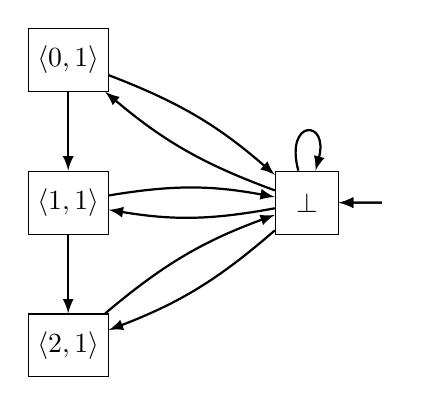
\begin{tikzpicture} [scale=1.2, every initial by arrow/.style={thick}]
%		\newcommand{\varstyle}[2]{\mt{\langle#1,#2\rangle}};

		\node [gstate](s01) at (0,0) {\varstyle{0}{1}};
		\node [gstate,below=of s01] (s11){\varstyle{1}{1}};
		\node [gstate,below=of s11] (s21){\varstyle{2}{1}};
		
		\node [gstate,initial,initial right,initial text=,right=60pt of s11] (sbot){$\notppty$};
		
		\path [trans] (s01) edge (s11);
		\path [trans] (s11) edge (s21);
		\path [bendtrans] (sbot) edge (s01);
		\path [bendtrans] (sbot) edge (s11);
		\path [bendtrans] (sbot) edge (s21);
		\path [bendtrans] (s01) edge (sbot);
		\path [bendtrans] (s11) edge (sbot);
		\path [bendtrans] (s21) edge (sbot);
		
		\path [trans] (sbot) edge [loop above] (sbot);
		
		%		midway, at start, near start, very near start, at end, near end, very near end
		
		
	\end{tikzpicture}
\end{document}
	\end{minipage}
	\caption{Simplified representations of \mdp (left) and the \viewN \viewdistance on it (right)}
	\label{fig:varsValEq}  
\end{figure}

Analogously a view that requires inequality instead of equality is feasible.

%\begin{definition}
%	Let $\chgph = \chgphtuple$ be \achgphN, $\var \in \vars$ and $\varval \in \varevalimg$. The view \viewparamvaluesneq is defined by its \grpfctN $\gfctparamvaluesneq : \states \to \imggrp$ with
%	\[
%	\state \mapsto
%	\begin{cases}
%			\group, &\text{if } \vareval(\state, \var) \neq \varval\\
%			\remelem, 	&\text{otherwise}
%		\end{cases}
%	\]
%	where $\imggrp := \imggrpbinview$.
%\end{definition}

If states are to be grouped with the requirement of several variables equaling or not equaling specified values this can be achieved by using \parllcompN.

To allow even more flexibility a view can be used that also allows a combination of requirements on variables in a disjunctive manner. To extend this idea to its full potential we will define a \viewN that allows requirements using a disjunctive normal formal (DNF). To formalize this view more efficiently we will write $\varstate[,i]$ short for $\vareval(\state, \var_i)$ where $x_i \in \vars$ and $i \in \natnums$. We define the symbol \eqorneq to be an element of the set $\{=,\neq\}$. That is to say, whenever it is used each time written it is a representative for either the symbol $=$ or $\neq$. It allows to write one symbol whenever $=$ and $\neq$ could or should be possible. Moreover for this context we consider $(\varstate[,i] = \varval)$ as a literal and $(\varstate[,i] \neq \varval)$ as its negation. We write $(\varstate[,i] \eqorneq \varval)$ for a literal that could be negated or not negated.

\begin{definition}
	Let $\chgph = \chgphtuple$ be \achgphN and 
	\begin{align*}
		c(s) = &((\varstate[,i_1] \eqorneq \varval_{i_1}) \land \dots \land (\varstate[,i_{l_1}] \eqorneq \varval_{i_{l_1}})) \; \lor \\
		&((\varstate[,i_{l_1+1}] \eqorneq \varval_{i_{l_1+1}}) \land \dots \land (\varstate[,i_{l_2}] \eqorneq \varval_{i_{l_2}})) \; \lor  \\
		&\dots \\ 
		&((\varstate[,i_{(l_{m-1})+1}] \eqorneq \varval_{i_{(l_{m-1})+1}}) \land \dots \land (\varstate[,i_{l_m}]  \eqorneq \varval_{i_{l_m}}))
	\end{align*}
	
	proposition logical formula in disjunctive normal form where
	\begin{itemize}
		\item $\varstate[,i_k], a_{i_k} \in \varevalimg$ with $i_k\in \natnums$ and $k \in \{1, \dots, l_m\}$
		\item $l_1 < l_2 < \dots < l_m$ are natural numbers and $m$ is the number of clauses in $c(s)$
	\end{itemize}		
	The \viewN \viewparamdnf is defined by its \grpfctN $\gfctparamdnf : \states \to \imggrp$ with
	\[
	\state \mapsto
	\begin{cases}
			\group, &\text{if } d(s) \text{ is true}\\
			\remelem, 	&\text{otherwise}
		\end{cases}
	\]
	
	where $\imggrp := \{\group, \remelem\}$.
\end{definition}


The DNF allows us to specify a requirement in disjunctive normal form about variables. States are mapped to the same value depending on whether or not they meet this requirement.

\redcomment{DISCUSSION OF EQUALITY, EQ CLASSES AND RESULTING STATES MISSING}

\begin{figure}[h]
	\begin{minipage}{.6\textwidth}
		%		\hspace{5mm}		
		\documentclass[tikz]{standalone}
%\usepackage{prelude}

%%%%%%%%%%%%%%%%%%%%%%%%%%%%%%%%%%%% PACKAGES %%%%%%%%%%%%%%%%%%%%%%%%%%%%%%%%%%%%%%%%%%

\usepackage{inputenc,fontenc}
\usepackage[a4paper,margin=3cm]{geometry}
\usepackage[english]{babel}
%\usepackage[german]{babel}
%\usepackage[fixlanguage]{babelbib}


\usepackage{bbold}
\usepackage{amsthm}
\usepackage{amsmath}
\usepackage{amssymb} % doteqdot
\usepackage[dvipsnames]{xcolor}
\usepackage{standalone}
\usepackage{tikz}[mode=buildnew]
\usepackage{cite}
\usepackage{xspace}
\usepackage{relsize}
\usepackage{mathtools} % mathclap
%\usepackage{MnSymbol}
\usepackage{hyperref}
\usepackage{url}
\usepackage{listings} % for code
\usepackage[T1]{fontenc} %<
\hypersetup{
	colorlinks,
	citecolor=black,
	filecolor=black,
	linkcolor=black,
	urlcolor=black
}
\usepackage{pgfplots}
\pgfplotsset{compat=1.18}
%\usepackage{courier} %% Sets font for listing as Courier. But also for url and texttt!
\usepackage{listings, xcolor}
\usepackage{graphicx}
\usepackage{subcaption}

\usetikzlibrary{calc}
%\usepackage{xparse} % \newDocumentCommand for multiple optional arguments
%\usepackage{titlecaps}



%%%%%%%%%%%%%%%%%%%%%%%%%%%%%%%%%%%% THEOREMSTYLES %%%%%%%%%%%%%%%%%%%%%%%%%%%%%%%%%%

\theoremstyle{definition}
\newtheorem{definition}{Definition}[section]
\newtheorem{exmp}{Beispiel}[section]
%\AfterEndEnvironment{definition}{\noindent\ignorespaces}

\theoremstyle{theorem}
\newtheorem{theorem}{Satz}[section]
\newtheorem{proposition}{Proposition}[section]
%\AfterEndEnvironment{theorem}{\noindent\ignorespaces}

\theoremstyle{korollary}
\newtheorem{korollary}{Korollar}[section]
%\AfterEndEnvironment{korollary}{\noindent\ignorespaces}


\tikzset{
	mstate/.style={draw, circle, minimum size=.94cm}, 
	gstate/.style={draw, rectangle, minimum size=.8cm},
	varstate/.style={draw,rectangle, rounded corners, minimum size=1}, 
	trans/.style={draw, ->, thick},
	bendtrans/.style={draw, ->, thick, bend left=10},
	bendtransr/.style={draw, ->, thick, bend right=10},
	init/.style={initial, initial distance=6pt, initial text=},
	every loop/.style={min distance=5pt, looseness=8},
	>=latex
}
\usetikzlibrary{automata,positioning}

%auto shift/.style={auto=right,->,
%	to path={ let \p1=(\tikztostart),\p2=(\tikztotarget),
%		\n1={atan2(\y2-\y1,\x2-\x1)},\n2={\n1+180}
%		in ($(\tikztostart.{\n1})!1mm!270:(\tikztotarget.{\n2})$) -- 
%		($(\tikztotarget.{\n2})!1mm!90:(\tikztostart.{\n1})$) \tikztonodes}},

%%%%%%%%%%%%%%%%%%%%%%%%%%%%%%%%%%% MY MACROS %%%%%%%%%%%%%%%%%%%%%%%%%%%%%%%%%%%%%%%%%
%formatting
\newcommand{\comment}[2]{{\color{#1}#2}}
\newcommand{\redcomment}[1]{{\color{red}#1}}
\newcommand{\purpcomment}[1]{{\color{pink}#1}}
\newcommand{\bluecomment}[1]{{\color{blue}#1}}
\newcommand{\mt}[1]{\ensuremath{{#1}}\xspace}
\newcommand{\mynewcommand}[2]{\newcommand{#1}{\mt{#2}}} %% currently not used becaue of ide highlighting
\newcommand{\arr}{\mt{\to}}

%model checking terms
\newcommand{\mimicrel}{\mt{\mathcal{R}}}
\newcommand{\bisimeq}{\mt{\;\!\sim\;\!}}
\newcommand{\simorder}{\mt{\;\!\preceq\;\!}}
\newcommand{\simequiv}{\mt{\;\!\simeq\;\!}} %command already defined
\newcommand{\relts}{\mt{\;\!\bullet_{_{\tiny{TS}}}\;\!}}
\newcommand{\rel}{\mt{\;\!\bullet\;\!}}

%own names
\newcommand{\nm}[1]{#1\xspace}
\newcommand{\mdpN}{\nm{MDP}}
\newcommand{\mdpsN}{\nm{MDPs}}
\newcommand{\viewN}{\nm{view}}
\newcommand{\viewNC}{\nm{View}}
\newcommand{\viewsN}{\nm{views}}
\newcommand{\viewsNC}{\nm{Views}}
\newcommand{\grpfctsubN}{\nm{detached grouping function}}
\newcommand{\grpfctsubNC}{\nm{detached grouping function}}
\newcommand{\grpfctsubNCC}{\nm{Detached Grouping Function}}
\newcommand{\grpfctN}{\nm{grouping function}}
\newcommand{\grpfctNC}{\nm{Grouping function}}
\newcommand{\grpfctNCC}{\nm{Grouping Function}}
\newcommand{\grpfctsN}{\nm{grouping functions}}
\newcommand{\grpfctsNC}{\nm{Grouping functions}}
\newcommand{\grpfctsNCC}{\nm{Grouping Functions}}
\newcommand{\stmimicN}{\nm{state-mimic}}
\newcommand{\stmimicsN}{\nm{state-mimics}}
\newcommand{\stmimickingN}{\nm{state-mimicking}}
\newcommand{\stmimickedN}{\nm{state-mimicked}}
%\newcommand{\chosenphtypeNCC}{\nm{Transition System}}
%\newcommand{\chgphNC}{\nm{Transition system}}
%\newcommand{\chgphN}{\nm{transition system}}
%\newcommand{\chgphsNCC}{\nm{Transition Systems}}
%\newcommand{\chgphsNC}{\nm{Transition systems}}
%\newcommand{\chgphsN}{\nm{transition systems}}
\newcommand{\chgphNCC}{\nm{MDP}}
\newcommand{\chgphNC}{\nm{MDP}}
\newcommand{\chgphN}{\nm{MDP}}
\newcommand{\achgphN}{\nm{an MDP}}
\newcommand{\chgphsNCC}{\nm{MDPs}}
\newcommand{\chgphsNC}{\nm{MDPs}}
\newcommand{\chgphsN}{\nm{MDPs}}
\newcommand{\parllcompN}{\nm{parallel composition}}
\newcommand{\parllcompNC}{\nm{Parallel composition}}
\newcommand{\parllcompNCC}{\nm{Parallel Composition}}
\newcommand{\parllcompsN}{\nm{parallel compositions}}
\newcommand{\parllcompsNC}{\nm{Parallel compositions}}
\newcommand{\parllcompsNCC}{\nm{Parallel Compositions}}
\newcommand{\sccN}{\nm{SCC}}
\newcommand{\sccsN}{\nm{SCCs}}
\newcommand{\bsccN}{\nm{BSCC}}
\newcommand{\bsccsN}{\nm{BSCCs}}
\newcommand{\jgrapht}{\nm{jGraphtT}}

\newcommand{\outactident}{\nm{OutActionsIdent}}

%names
\newcommand{\iffN}{\nm{if and only if}}
\newcommand{\tsN}{\nm{TS}}

%% outactions identical
\newcommand{\outactidentstrong}{\nm{strong}}
\newcommand{\outactidentweak}{\nm{weak}}

% CORE DEFINITIONS
\newcommand{\grpfct}[1][\viewppty]{\mt{F_{#1}}}
\newcommand{\grpfctsub}[1][\viewppty]{\mt{\tilde{F}_{#1}}}
%\newcommand{\grpfctimg}[1]{\mt{{\grpfct}[{#1}]}}
%\newcommand{\fctimg}[2]{\mt{{#1}[{#2}]}}
\newcommand{\eqrelview}{\mt{R}}
\newcommand{\eqclassv}[1][\state]{\mt{\eqclass{#1}{\eqrelview}}}
\newcommand{\eqclasssetv}[1][\states]{\mt{{#1}/\eqrelview}} %OLD: \bigcup_{\state \in \states} \eqclassv
\newcommand{\viewid}{\mt{\mdp}}
\newcommand{\view}[1][\viewppty]{\mt{\viewid_{#1}}}
\newcommand{\imggrp}{\mt{\arbset}}
\newcommand{\imggrpsub}{\mt{X}}
\newcommand{\viewppty}{\mt{\theta}}
\newcommand{\pll}{\mt{\;\!\pllpure\;\!}}
\newcommand{\pllrev}{\mt{\pllpure^{-1}}}
\newcommand{\pllpure}{\mt{||}}
\newcommand{\compselectset}{\mt{Z}}
\newcommand{\compselectpure}{\mt{\pllpure_\compselectset}}
\newcommand{\compselect}{\mt{\;\pllpure_\compselectset\;}}
\newcommand{\remstates}{\mt{\bigcup_{\state \in \states \setminus \states_1}\{\{\state\}\}}}
\newcommand{\nogroupstates}[1][\states_2]{\mt{\bigcup_{\state \in \states \setminus {#1}}\{\{\state\}\}}}
\newcommand{\remelem}{\mt{\bullet}}
\newcommand{\nogroupset}{\mt{\xi}}
\newcommand{\remset}{\mt{\{\remelem\}}}
\newcommand{\gfctpll}{\mt{\grpfct[\pll]}}
\newcommand{\group}{\mt{\top}}
\newcommand{\imggrpbinview}{\mt{\{\remelem, \notppty\}}}
\newcommand{\viewappset}{\mt{\tilde{\states}}}
\newcommand{\hasppty}{\mt{\top}}
\newcommand{\notppty}{\mt{\bot}}
\newcommand{\disregardelem}{\mt{\Delta}}
\newcommand{\disregardelements}{\mt{{\disregardelem_1, \dots, \disregardelem_n}}}



%\newcommand{\mdp}{def}\mdp
%\newcommand{\mdpdef}



% EXAMPLE VIEWS
\newcommand{\pptyatomicprops}{\mt{\atomicprops}}
\newcommand{\pptyinitstates}{\mt{\initstates}}
\newcommand{\pptyinactsetsize}{\mt{|\inacts(\state)|}}
\newcommand{\pptyhasoutact}{\mt{\exists\outact}}
\newcommand{\pptyminoutact}[2]{\mt{#1\leq#2}}
\newcommand{\pptymaxoutact}[2]{\mt{#2\leq#1}}
\newcommand{\pptyspanoutact}[3]{\mt{#1\leq#2\leq#3}}
\newcommand{\pptyoutactsetsize}{\mt{|\outacts(\state)|}}
\newcommand{\pptyoutactsingle}{\mt{|\outacts(\state)|_1}}
\newcommand{\pptystrongoutactident}{\mt{\outacts(\state)_=}}
\newcommand{\pptyweakoutactident}{\mt{\outacts(\state)_\approx}}
\newcommand{\pptyhasinact}{\mt{\exists\inact}}
\newcommand{\pptymininact}[2]{\mt{#1\leq#2}}
\newcommand{\pptymaxinact}[2]{\mt{#2\leq#1}}
\newcommand{\pptyspaninact}[3]{\mt{#1\leq#2\leq#3}}
\newcommand{\pptyinactsingle}{\mt{|\inacts(\state)|_1}}
\newcommand{\pptystronginactident}{\mt{\inacts(\state)_=}}
\newcommand{\pptyweakinactident}{\mt{\inacts(\state)_\approx}}
\newcommand{\pptyparamvalueseq}{\mt{\var = \varval}}
\newcommand{\pptyparamvaluesneq}{\mt{\var \neq \varval}}
\newcommand{\pptyparamdnf}{\mt{VarDNF}}
\newcommand{\pptyparamcnf}{\mt{VarCNF}}
\newcommand{\pptyparamvalueseqopt}{\mt{\var = \varval}}
\newcommand{\pptyparamvalident}{\mt{Var:\varval}}
\newcommand{\pptydistance}{\mt{\distpath}}
\newcommand{\pptydistancerev}{\mt{\distpathrev}}
\newcommand{\pptydistancebi}{\mt{\distpathbi}}
\newcommand{\pptyhascycle}{\mt{\exists\cycle}}
\newcommand{\pptyexactactcycle}{\mt{\{\cycle_{\action,n}\}}}
\newcommand{\pptycycleset}{\mt{\cup{\{\state\}_\cycle}}}
\newcommand{\pptyexactcycle}{\mt{\{\cycle_n\}}}
\newcommand{\pptyscc}{\mt{scc}}
\newcommand{\pptybscc}{\mt{bscc}}
\newcommand{\pptyprop}{\mt{\redcomment{?}}}
\newcommand{\pptyident}{id}


\newcommand{\gfctatomicprops}{\mt{\grpfct[\pptyatomicprops]}}
\newcommand{\gfctinitstates}{\mt{\grpfct[\pptyinitstates]^\hasppty}}
\newcommand{\gfcthasoutaction}{\mt{\grpfct[\pptyhasoutact]^\hasppty}}
\newcommand{\gfctminoutaction}{\mt{\grpfct[\pptyminoutact{\numoutact}{\outact}]^\hasppty}}
\newcommand{\gfctmaxoutaction}{\mt{\grpfct[\pptymaxoutact{\numoutact}{\outact}]^\hasppty}}
\newcommand{\gfctspanoutaction}{\mt{\grpfct[\pptyspanoutact{\numoutactb}{\outact}{\numoutact}]^\hasppty}}
\newcommand{\gfctoutactsetsize}{\mt{\grpfct[\pptyoutactsetsize]}}
\newcommand{\gfctoutactsingle}{\mt{\grpfct[\pptyoutactsingle]^\notppty}}
\newcommand{\gfctstrongoutactident}{\mt{\grpfct[\pptystrongoutactident]}}
\newcommand{\gfctweakoutactident}{\mt{\grpfct[\pptyweakoutactident]}}
\newcommand{\gfcthasinaction}{\mt{\grpfct[\pptyhasinact]^\hasppty}}
\newcommand{\gfctmininaction}{\mt{\grpfct[\pptymininact{\numinact}{\inact}]^\hasppty}}
\newcommand{\gfctmaxinaction}{\mt{\grpfct[\pptymaxinact{\numinact}{\inact}]^\hasppty}}
\newcommand{\gfctspaninaction}{\mt{\grpfct[\pptyspaninact{\numinactb}{\inact}{\numinact}]^\hasppty}}
\newcommand{\gfctinactsetsize}{\mt{\grpfct[\pptyinactsetsize]}}
\newcommand{\gfctinactsingle}{\mt{\grpfct[\pptyinactsingle]^\notppty}}
\newcommand{\gfctstronginactident}{\mt{\grpfct[\pptystronginactident]}}
\newcommand{\gfctweakinactident}{\mt{\grpfct[\pptyweakinactident]}}
\newcommand{\gfctparamvalueseq}{\mt{\grpfct[\pptyparamvalueseq]^\hasppty}}
\newcommand{\gfctparamvaluesneq}{\mt{\grpfct[\pptyparamvaluesneq]^\hasppty}}
\newcommand{\gfctparamdnf}{\mt{\grpfct[\pptyparamdnf]^\hasppty}}
\newcommand{\gfctparamcnf}{\mt{\grpfct[\pptyparamcnf]^\hasppty}}
\newcommand{\gfctparamvalueseqopt}{\mt{\pptyparamvalueseqopt}}
\newcommand{\gfctparamvalident}{\mt{\grpfct[\pptyparamvalident]}}
\newcommand{\gfctdistance}{\mt{\grpfct[\pptydistance]}}
\newcommand{\gfctdistancerev}{\mt{\grpfct[\pptydistancerev]}}
\newcommand{\gfctdistancebi}{\mt{\grpfct[\pptydistancebi]}}
\newcommand{\gfcthascycle}{\mt{\grpfct[\pptyhascycle]}}
\newcommand{\gfctexactcycle}{\mt{\grpfct[\pptyexactcycle]}}
\newcommand{\gfctcycleset}{\mt{\grpfct[\pptycycleset]}}
\newcommand{\gfctexactactcycle}{\mt{\grpfct[\pptyexactactcycle]}}
\newcommand{\gfctscc}{\mt{\grpfct[\pptyscc]}}
\newcommand{\gfctbscc}{\mt{\grpfct[\pptybscc]}}
\newcommand{\gfctprop}{\mt{\grpfct[\pptyprop]}}
\newcommand{\gfctident}{\mt{\grpfct[\pptyident]}}

\newcommand{\gfctsubatomicprops}{\mt{\grpfctsub[\pptyatomicprops]}}
\newcommand{\gfctsubinitstates}{\mt{\grpfctsub[\pptyinitstates]^\hasppty}}
\newcommand{\gfctsubhasoutaction}{\mt{\grpfctsub[\pptyhasoutact]^\hasppty}}
\newcommand{\gfctsubminoutaction}{\mt{\grpfctsub[\pptyminoutact{\numoutact}{\outact}]^\hasppty}}
\newcommand{\gfctsubmaxoutaction}{\mt{\grpfctsub[\pptymaxoutact{\numoutact}{\outact}]^\hasppty}}
\newcommand{\gfctsubspanoutaction}{\mt{\grpfctsub[\pptyspanoutact{\numoutactb}{\outact}{\numoutact}]^\hasppty}}
\newcommand{\gfctsuboutactsetsize}{\mt{\grpfctsub[\pptyoutactsetsize]}}
\newcommand{\gfctsuboutactsingle}{\mt{\grpfctsub[\pptyoutactsingle]^\notppty}}
\newcommand{\gfctsubstrongoutactident}{\mt{\grpfctsub[\pptystrongoutactident]^\hasppty}}
\newcommand{\gfctsubweakoutactident}{\mt{\grpfctsub[\pptyweakoutactident]^\hasppty}}
\newcommand{\gfctsubhasinaction}{\mt{\grpfctsub[\pptyhasinact]}}
\newcommand{\gfctsubmininaction}{\mt{\grpfctsub[\pptymininact{\numinact}{\inact}]}}
\newcommand{\gfctsubmaxinaction}{\mt{\grpfctsub[\pptymaxinact{\numinact}{\inact}]}}
\newcommand{\gfctsubspaninaction}{\mt{\grpfctsub[\pptyspaninact{\numinactb}{\inact}{\numinact}]}}
\newcommand{\gfctsubinactsetsize}{\mt{\grpfctsub[\pptyinactsetsize]^\hasppty}}
\newcommand{\gfctsubinactsingle}{\mt{\grpfctsub[\pptyinactsingle]^\notppty}}
\newcommand{\gfctsubstronginactident}{\mt{\grpfctsub[\pptystronginactident]}}
\newcommand{\gfctsubweakinactident}{\mt{\grpfctsub[\pptyweakinactident]}}
\newcommand{\gfctsubparamvalueseq}{\mt{\grpfctsub[\pptyparamvalueseq]^\hasppty}}
\newcommand{\gfctsubparamvaluesneq}{\mt{\grpfctsub[\pptyparamvaluesneq]^\hasppty}}
\newcommand{\gfctsubparamdnf}{\mt{\grpfctsub[\pptyparamdnf]^\hasppty}}
\newcommand{\gfctsubparamcnf}{\mt{\grpfctsub[\pptyparamcnf]^\hasppty}}
\newcommand{\gfctsubparamvalueseqopt}{\mt{\pptyparamvalueseqopt}}
\newcommand{\gfctsubparamvalident}{\mt{\grpfctsub[\pptyparamvalident]}}
\newcommand{\gfctsubdistance}{\mt{\grpfctsub[\pptydistance]}}
\newcommand{\gfctsubdistancerev}{\mt{\grpfctsub[\pptydistancerev]}}
\newcommand{\gfctsubdistancebi}{\mt{\grpfctsub[\pptydistancebi]}}
\newcommand{\gfctsubhascycle}{\mt{\grpfctsub[\pptyhascycle]^\hasppty}}
\newcommand{\gfctsubexactcycle}{\mt{\grpfctsub[\pptyexactcycle]}}
\newcommand{\gfctsubcycleset}{\mt{\grpfctsub[\pptycycleset]}}
\newcommand{\gfctsubexactactcycle}{\mt{\grpfctsub[\pptyexactactcycle]}}
\newcommand{\gfctsubscc}{\mt{\grpfctsub[\pptyscc]}}
\newcommand{\gfctsubbscc}{\mt{\grpfctsub[\pptybscc]}}
\newcommand{\gfctsubprop}{\mt{\grpfctsub[\pptyprop]}}
\newcommand{\gfctsubident}{\mt{\grpfctsub[\pptyident]}}


\newcommand{\viewatomicprops}{\mt{\view[\pptyatomicprops]}}
\newcommand{\viewinitstates}{\mt{\view[\pptyinitstates]^\hasppty}}
\newcommand{\viewhasoutaction}{\mt{\view[\pptyhasoutact]^\hasppty}}
\newcommand{\viewminoutaction}{\mt{\view[\pptyminoutact{\numoutact}{\outact}]^\hasppty}}
\newcommand{\viewmaxoutaction}{\mt{\view[\pptymaxoutact{\numoutact}{\outact}]^\hasppty}}
\newcommand{\viewspanoutaction}{\mt{\view[\pptyspanoutact{\numoutactb}{\outact}{\numoutact}]^\hasppty}}
\newcommand{\viewoutactsetsize}{\mt{\view[\pptyoutactsetsize]}}
\newcommand{\viewoutactsingle}{\mt{\view[\pptyoutactsingle]^\notppty}}
\newcommand{\viewstrongoutactident}{\mt{\view[\pptystrongoutactident]}}
\newcommand{\viewweakoutactident}{\mt{\view[\pptyweakoutactident]}}
\newcommand{\viewhasinaction}{\mt{\view[\pptyhasinact]^\hasppty}}
\newcommand{\viewmininaction}{\mt{\view[\pptymininact{\numinact}{\inact}]^\hasppty}}
\newcommand{\viewmaxinaction}{\mt{\view[\pptymaxinact{\numinact}{\inact}]^\hasppty}}
\newcommand{\viewspaninaction}{\mt{\view[\pptyspaninact{\numinactb}{\inact}{\numinact}]^\hasppty}}
\newcommand{\viewinactsetsize}{\mt{\view[\pptyinactsetsize]}}
\newcommand{\viewinactsingle}{\mt{\view[\pptyinactsingle]^\notppty}}
\newcommand{\viewstronginactident}{\mt{\view[\pptystronginactident]}}
\newcommand{\viewweakinactident}{\mt{\view[\pptyweakinactident]}}
\newcommand{\viewparamvalueseq}{\mt{\view[\pptyparamvalueseq]}}
\newcommand{\viewparamvaluesneq}{\mt{\view[\pptyparamvaluesneq]}}
\newcommand{\viewparamdnf}{\mt{\view[\pptyparamdnf]^\hasppty}}
\newcommand{\viewparamcnf}{\mt{\view[\pptyparamcnf]^\hasppty}}
\newcommand{\viewparamvalueseqopt}{\mt{\pptyparamvalueseqopt}}
\newcommand{\viewparamvalident}{\mt{\view[\pptyparamvalident]}}
\newcommand{\viewdistance}{\mt{\view[\pptydistance]}}
\newcommand{\viewdistancerev}{\mt{\view[\pptydistancerev]}}
\newcommand{\viewdistancebi}{\mt{\view[\pptydistancebi]}}
\newcommand{\viewhascycle}{\mt{\view[\pptyhascycle]}}
\newcommand{\viewexactcycle}{\mt{\view[\pptyexactcycle]}}
\newcommand{\viewcycleset}{\mt{\view[\pptycycleset]}}
\newcommand{\viewexactactcycle}{\mt{\view[\pptyexactactcycle]}}
\newcommand{\viewscc}{\mt{\view[\pptyscc]}}
\newcommand{\viewbscc}{\mt{\view[\pptybscc]}}
\newcommand{\viewprop}{\mt{\view[\pptyprop]}}
\newcommand{\viewident}{\mt{\view[\pptyident]}}

%\newcommand{\viewatomicprops}{\mt{\view[\atomicprops]}}
%\newcommand{\viewinitstates}{\mt{\view[\initstates]}}
%\newcommand{\viewhasoutaction}{\mt{\view[\pptyhasoutact]}}
%\newcommand{\viewminoutaction}{\mt{\view[\pptyminoutact{\numoutact}{\outact}]}}
%\newcommand{\viewmaxoutaction}{\mt{\view[\pptymaxoutact{\numoutact}{\outact}]}}
%\newcommand{\viewspanoutaction}{\mt{\view[\pptyspanoutact{\numoutactb}{\outact}{\numoutact}]}}
%\newcommand{\viewoutactsetsize}{\mt{\view[\pptyoutactsetsize]}}
%\newcommand{\viewoutactsingle}{\mt{\view[\pptyoutactsingle]}}
%\newcommand{\viewstrongoutactident}{\mt{\view[\outacts(\state)_=]}}
%\newcommand{\viewweakoutactident}{\mt{\view[\outacts(\state)_\approx]}}
%\newcommand{\viewhasinaction}{\mt{\view[\pptyhasinact]}}
%\newcommand{\viewmininaction}{\mt{\view[\pptymininact{\numinact}{\inact}]}}
%\newcommand{\viewmaxinaction}{\mt{\view[\pptymaxinact{\numinact}{\inact}]}}
%\newcommand{\viewspaninaction}{\mt{\view[\pptyspaninact{\numinactb}{\inact}{\numinact}]}}
%\newcommand{\viewinactsetsize}{\mt{\view[\pptyinactsetsize]}}
%\newcommand{\viewinactsingle}{\mt{\view[\pptyinactsingle]}}
%\newcommand{\viewstronginactident}{\mt{\view[\inacts(\state)_=]}}
%\newcommand{\viewweakinactident}{\mt{\view[\inacts(\state)_\approx]}}
%\newcommand{\viewparamvalueseq}{\mt{\view[\var = \varval]}}
%\newcommand{\viewparamvaluesneq}{\mt{\view[\var \neq \varval]}}
%\newcommand{\viewparamdnf}{\mt{\view[VarDNF]}}
%\newcommand{\viewparamcnf}{\mt{\view[VarCNF]}}
%\newcommand{\viewparamvalident}{\mt{\view[\pptyparamvalident]}}
%\newcommand{\viewdistance}{\mt{\view[\pptydistance]}}
%\newcommand{\viewhascycle}{\mt{\view[\exists\cycle]}}
%\newcommand{\viewexactcycle}{\mt{\view[\pptyexactcycle]}}
%\newcommand{\viewcycleset}{\mt{\view[\pptycycleset]}}
%\newcommand{\viewexactactcycle}{\mt{\view[\pptyexactactcycle]}}
%\newcommand{\viewscc}{\mt{\view[scc]}}
%\newcommand{\viewbscc}{\mt{\view[bscc]}}

%actions
\newcommand{\numoutact}{\mt{n}}
\newcommand{\numoutactb}{\mt{m}}
\newcommand{\numinact}{\mt{n}}
\newcommand{\numinactb}{\mt{m}}

\newcommand{\predmaxoutact}[1][\numoutact]{\mt{Q_{\outact\leq#1}(\state,\state_1, \dots, \state_{#1+1})}}
\newcommand{\predminoutact}[1][\numoutact]{\mt{Q_{#1\leq\outact}(\state,\state_1, \dots, \state_{#1})}}
\newcommand{\formoutact}[1][\state]{\mt{C_{#1,\outact}}}
\newcommand{\predmaxinact}[1][\numinact]{\mt{Q_{\inact\leq#1}(\state,\state_1, \dots, \state_{#1+1})}}
\newcommand{\predmininact}[1][\numinact]{\mt{Q_{#1\leq\inact}(\state,\state_1, \dots, \state_{#1})}}

\newcommand{\outact}[1][\action]{\mt{\overrightarrow{#1}}}
\newcommand{\outacts}{\mt{\overrightarrow{\actions}}}
\newcommand{\inact}{\mt{\overleftarrow{\action}}}
\newcommand{\inacts}[1][\action]{\mt{\overleftarrow{#1}}}

%%Parameters
\newcommand{\vars}[1][\mdp]{\mt{V\!ar_{#1}}}
\newcommand{\var}{\mt{x}}
\newcommand{\varstate}[1][]{\mt{\var_{\state#1}}}
\newcommand{\varval}{\mt{a}}
\newcommand{\vareval}[1][\mdp]{\mt{V\!arEval_{#1}}}
\newcommand{\varevalimg}[1][\mdp]{\mt{\vareval[#1][\states,\vars]}}
\newcommand{\varevalimgset}{\mt{\arbset}}
\newcommand{\someparam}{\mt{\tilde{x}}}
\newcommand{\eqorneq}{\mt{\;\doteqdot\;}}
\newcommand{\varstyle}[2]{\mt{\langle#1,#2\rangle}}




%\makeatletter
%\newcommand{\overleftrightsmallarrow}{\mathpalette{\overarrowsmall@\leftrightarrowfill@}}
%\newcommand{\overrightsmallarrow}{\mathpalette{\overarrowsmall@\rightarrowfill@}}
%\newcommand{\overleftsmallarrow}{\mathpalette{\overarrowsmall@\leftarrowfill@}}
%\newcommand{\overarrowsmall@}[3]{%
%	\vbox{%
%		\ialign{%
%			##\crcr
%			#1{\smaller@style{#2}}\crcr
%			\noalign{\nointerlineskip}%
%			$\m@th\hfil#2#3\hfil$\crcr
%		}%
%	}%
%}
%\def\smaller@style#1{%
%	\ifx#1\displaystyle\scriptstyle\else
%	\ifx#1\textstyle\scriptstyle\else
%	\scriptscriptstyle
%	\fi
%	\fi
%}
%\makeatother
%\newcommand{\te}[1]{\overleftrightsmallarrow{#1}}

% Distance
\newcommand{\fctdist}{\mt{distance}}
\newcommand{\fctdistdefault}{\mt{\fctdist(\chgph, \smstates, \grandist)}}
\newcommand{\distval}{\mt{d}}
\newcommand{\grandist}{\mt{n}}
\let\path\oldpath
\newcommand{\path}{\mt{P}}
\newcommand{\pathbi}{\mt{\bar{\path}}}
\newcommand{\pathsecfull}{\mt{(\state_0, \action_0, \state_1, \action_1, \dots, \action_{n}, \state_{n+1})}}
\newcommand{\lenpath}{\mt{len}}
\newcommand{\pfirst}{\mt{first}}
\newcommand{\plast}{\mt{last}}
\newcommand{\pathset}{\mt{\path_\chgph}}
\newcommand{\pathbiset}{\mt{\pathbi_\chgph}}
\newcommand{\distpath}{\mt{\overrightarrow{dist}}}
\newcommand{\distpathrev}{\mt{\overleftarrow{dist}}}
\newcommand{\distpathbi}{\mt{\overline{dist}}}
%Cycles
\newcommand{\cyclesecfull}{\mt{(\state_0, \action_0, \state_1, \action_1, \dots, \action_{n-1}, \state_0)}}
\newcommand{\fctfindcycles}{\mt{findCycles}}
\newcommand{\cycle}{\mt{C}}
\newcommand{\cycleset}{\mt{\cycle_{\mdp, n}}}
\newcommand{\lencycle}{\mt{len}}
% strongly connected components
\newcommand{\scc}{\mt{T}}
\newcommand{\setscc}{\mt{SCC_{\chgph,n}}}
\newcommand{\setbscc}{\mt{BSCC_{\chgph,n}}}

% properties
\newcommand{\propfct}{\mt{f}}

% all Systems
\newcommand{\chgph}{\mt{\mdp}}
\newcommand{\chgphtuple}{\mt{\mdptuple}}
\newcommand{\chgphtupledist}{\mt{\mdptupledist}}

\newcommand{\states}{\mt{S}}
\newcommand{\actions}{\mt{Act}}
\newcommand{\atomicprops}{\mt{AP}}
\newcommand{\labelingfct}{\mt{L}}
\newcommand{\init}{\mt{\initdistrib}} % use MDP % refers to the underlying set
\newcommand{\trans}{\mt{\probtfunc}} % use MDP % refers to the underlying set
\newcommand{\smstates}{\mt{\tilde{\states}}}


\newcommand{\state}{\mt{s}}
\newcommand{\action}{\mt{\alpha}}
\newcommand{\actionb}{\mt{\beta}}
\newcommand{\actionc}{\mt{\gamma}}
\newcommand{\smstate}{\mt{\tilde{\state}}}



% transition sysstems
\newcommand{\ts}{\mt{TS}}
\newcommand{\transitionrel}{\mt{\longrightarrow}}
\newcommand{\initstates}{\mt{I}}
\newcommand{\transitionsystem}{\mt
	{(\states, \actions, \transitionrel, \initstates, \atomicprops, \labelingfct)}
}
\newcommand{\tstupledist}{\mt{(\states', \actions',\transitionrel', \initstates', \labelingfct')}}


%Markov chains and MDP
\newcommand{\mdp}{\mt{\autm}}
\newcommand{\mdptuple}{\mt{(\states, \actions, \probtfunc, \initdistrib, \atomicprops, \labelingfct)}}
\newcommand{\mdptupledist}{\mt{(\states', \actions', \probtfunc', \initdistrib', \atomicprops', \labelingfct')}}
\newcommand{\autm}{\mt{\mathcal{M}}}
\newcommand{\probtfunc}{\mt{\textbf{P}}}
\newcommand{\initdistrib}{\mt{\iota_{init}}}


%maths
\newcommand{\powerset}[1]{\mt{\mathcal{P}(#1)}}
\newcommand{\eqclass}[2]{\mt{[#1]_{#2}}}%{\mt{#1 / #2}}
\newcommand{\impr}{\mt{\hspace{3mm}\Rightarrow\hspace{2mm}}}
\newcommand{\impl}{\mt{\hspace{3mm}\Leftarrow\hspace{2mm}}}
\newcommand{\natnums}{\mt{\mathbb{N}}} 
\newcommand{\realnums}{\mt{\mathbb{R}}}
\newcommand{\intmodn}[1][n]{\mt{\mathbb{Z}_{#1}}}
\newcommand{\arbset}{\mt{M}}
\newcommand{\bigsum}[2][]{\mt{\mathlarger{\sum}_{#2}^{#1}}}
\newcommand{\bbigsum}[2][]{\mt{\mathlarger{\mathlarger{\sum}}_{#2}^{#1}}}
\newcommand{\invimage}[2]{#1^{\mt{-1}(#2)}}
\newcommand{\img}{\mt{Img}}
\newcommand{\cond}{\mt{\,|\,}}

%tickz
%% \definecolor{darkred}{RGB}{196, 42, 42}

%implementation
\newcommand{\pmcvis}{\nm{PMC-Vis}}


\usepackage{tikz}
\newcommand{\stateppty}{draw, circle, minimum size=1cm}
\usepackage{ifthen}


\begin{document}
	\newcommand{\createstate}[3]{\node[draw, circle, minimum size=1cm] (#1) at (#2) {#3}}
	\newcommand{\basex}{0}
	\newcommand{\basey}{0}
	\begin{tikzpicture} [scale=2, every initial by arrow/.style={thick}]
		\newcommand{\varstyle}[2]{\mt{\langle#1,#2\rangle}};
		%		\createstate{s1}{3,2+4}{$\state_1$};

		\node [varstate,init] (s00) at (0,0){\varstyle{0}{0}};
		\node [varstate,right=of s00] (s01) {\varstyle{0}{1}};
		\node [varstate,right=of s01] (s02) {\varstyle{0}{2}};
		\node [varstate,below=of s00] (s10) {\varstyle{1}{0}};
		\node [varstate,right=of s10] (s11) {\varstyle{1}{1}};
		\node [varstate,right=of s11] (s12) {\varstyle{1}{2}};
		\node [varstate,below=of s10] (s20) {\varstyle{2}{0}};
		\node [varstate,right=of s20] (s21) {\varstyle{2}{1}};
		\node [varstate,right=of s21] (s22) {\varstyle{2}{2}};
		
%		\foreach \x in {0,...,2} 
%			\foreach \y [evaluate=\y as \i using \y+1] in {0,...,1}				
%				{	
%					\path [trans] (s\x\y) edge (s\x\i);
%					};
					
		\path [trans] (s00) edge (s01);
		\path [trans] (s01) edge (s02);
		\path [trans] (s10) edge (s11);
		\path [trans] (s11) edge (s12);
		\path [trans] (s20) edge (s21);
		\path [trans] (s21) edge (s22);
		\path [trans] (s00) edge (s10);
		\path [trans] (s10) edge (s20);
		\path [trans] (s01) edge (s11);
		\path [trans] (s11) edge (s21);
		\path [trans] (s02) edge (s12);
		\path [trans] (s12) edge (s22);
		
		\path [trans] (s22) edge [loop below] (s22);
				
%		\foreach \y in {0,...,2} 
%			\foreach \x in {0,...,1} 
%				{\path [trans] (s\x\y) edge (s\x+1\y);};
		
		
%		\foreach \x in {0,...,4} {
%			\foreach \y in {\x,...,4} {
%				\x --["\ifthenelse{\x=3 \OR \y=3 \OR \x=\y}{}{\x\y}",sloped] \y;
%				}}};
		
		
		%		\node [mstate,below right=40pt and 30 pt of s2] (s5) {$\state_5$};
%		\node [mstate,below=of s3] (s6) {$\state_6$};
%		\node [mstate,right=55pt of s6] (s7) {$\state_7$};
%		\node [mstate,below left=20pt and 30pt of s1] (s8) {$\state_8$};
%		\node [mstate,below=20pt of s8] (s9) {$\state_9$};
%		%		\node [mstate,right=of s2] (s10) {$\state_{10}$};
%		\node [mstate,above=26pt of s5] (s10) {$\state_{10}$};
%		
%		
%		
%		\path [trans] (s1) edge (s2);
%		\path [trans] (s1) edge (s3);
%		\path [trans] (s1) edge (s3);
%		\path [trans] (s1) edge (s8);
%		\path [trans] (s2) edge (s4);
%		\path [trans] (s3) edge (s4);
%		\path [trans] (s3) edge (s6);
%		\path [trans] (s5) edge (s2);
%		\path [trans] (s5) edge (s6);
%		\path [trans] (s5) edge (s7);
%		\path [trans] (s6) edge (s7);
%		\path [trans] (s9) edge (s8);
%		\path [trans] (s9) edge (s6);
%		
%		\path [trans] (s2) edge [loop above] (s2);
%		\path [trans] (s7) edge [loop right] (s7);
%		\path [trans] (s9) edge [loop below] (s9);
%		
	\end{tikzpicture}
\end{document}
	\end{minipage}%
	\begin{minipage}{.5\textwidth}
		\documentclass[tikz,preview]{standalone}
%\usepackage{prelude}

%%%%%%%%%%%%%%%%%%%%%%%%%%%%%%%%%%%% PACKAGES %%%%%%%%%%%%%%%%%%%%%%%%%%%%%%%%%%%%%%%%%%

\usepackage{inputenc,fontenc}
\usepackage[a4paper,margin=3cm]{geometry}
\usepackage[english]{babel}
%\usepackage[german]{babel}
%\usepackage[fixlanguage]{babelbib}


\usepackage{bbold}
\usepackage{amsthm}
\usepackage{amsmath}
\usepackage{amssymb} % doteqdot
\usepackage[dvipsnames]{xcolor}
\usepackage{standalone}
\usepackage{tikz}[mode=buildnew]
\usepackage{cite}
\usepackage{xspace}
\usepackage{relsize}
\usepackage{mathtools} % mathclap
%\usepackage{MnSymbol}
\usepackage{hyperref}
\usepackage{url}
\usepackage{listings} % for code
\usepackage[T1]{fontenc} %<
\hypersetup{
	colorlinks,
	citecolor=black,
	filecolor=black,
	linkcolor=black,
	urlcolor=black
}
\usepackage{pgfplots}
\pgfplotsset{compat=1.18}
%\usepackage{courier} %% Sets font for listing as Courier. But also for url and texttt!
\usepackage{listings, xcolor}
\usepackage{graphicx}
\usepackage{subcaption}

\usetikzlibrary{calc}
%\usepackage{xparse} % \newDocumentCommand for multiple optional arguments
%\usepackage{titlecaps}



%%%%%%%%%%%%%%%%%%%%%%%%%%%%%%%%%%%% THEOREMSTYLES %%%%%%%%%%%%%%%%%%%%%%%%%%%%%%%%%%

\theoremstyle{definition}
\newtheorem{definition}{Definition}[section]
\newtheorem{exmp}{Beispiel}[section]
%\AfterEndEnvironment{definition}{\noindent\ignorespaces}

\theoremstyle{theorem}
\newtheorem{theorem}{Satz}[section]
\newtheorem{proposition}{Proposition}[section]
%\AfterEndEnvironment{theorem}{\noindent\ignorespaces}

\theoremstyle{korollary}
\newtheorem{korollary}{Korollar}[section]
%\AfterEndEnvironment{korollary}{\noindent\ignorespaces}


\tikzset{
	mstate/.style={draw, circle, minimum size=.94cm}, 
	gstate/.style={draw, rectangle, minimum size=.8cm},
	varstate/.style={draw,rectangle, rounded corners, minimum size=1}, 
	trans/.style={draw, ->, thick},
	bendtrans/.style={draw, ->, thick, bend left=10},
	bendtransr/.style={draw, ->, thick, bend right=10},
	init/.style={initial, initial distance=6pt, initial text=},
	every loop/.style={min distance=5pt, looseness=8},
	>=latex
}
\usetikzlibrary{automata,positioning}

%auto shift/.style={auto=right,->,
%	to path={ let \p1=(\tikztostart),\p2=(\tikztotarget),
%		\n1={atan2(\y2-\y1,\x2-\x1)},\n2={\n1+180}
%		in ($(\tikztostart.{\n1})!1mm!270:(\tikztotarget.{\n2})$) -- 
%		($(\tikztotarget.{\n2})!1mm!90:(\tikztostart.{\n1})$) \tikztonodes}},

%%%%%%%%%%%%%%%%%%%%%%%%%%%%%%%%%%% MY MACROS %%%%%%%%%%%%%%%%%%%%%%%%%%%%%%%%%%%%%%%%%
%formatting
\newcommand{\comment}[2]{{\color{#1}#2}}
\newcommand{\redcomment}[1]{{\color{red}#1}}
\newcommand{\purpcomment}[1]{{\color{pink}#1}}
\newcommand{\bluecomment}[1]{{\color{blue}#1}}
\newcommand{\mt}[1]{\ensuremath{{#1}}\xspace}
\newcommand{\mynewcommand}[2]{\newcommand{#1}{\mt{#2}}} %% currently not used becaue of ide highlighting
\newcommand{\arr}{\mt{\to}}

%model checking terms
\newcommand{\mimicrel}{\mt{\mathcal{R}}}
\newcommand{\bisimeq}{\mt{\;\!\sim\;\!}}
\newcommand{\simorder}{\mt{\;\!\preceq\;\!}}
\newcommand{\simequiv}{\mt{\;\!\simeq\;\!}} %command already defined
\newcommand{\relts}{\mt{\;\!\bullet_{_{\tiny{TS}}}\;\!}}
\newcommand{\rel}{\mt{\;\!\bullet\;\!}}

%own names
\newcommand{\nm}[1]{#1\xspace}
\newcommand{\mdpN}{\nm{MDP}}
\newcommand{\mdpsN}{\nm{MDPs}}
\newcommand{\viewN}{\nm{view}}
\newcommand{\viewNC}{\nm{View}}
\newcommand{\viewsN}{\nm{views}}
\newcommand{\viewsNC}{\nm{Views}}
\newcommand{\grpfctsubN}{\nm{detached grouping function}}
\newcommand{\grpfctsubNC}{\nm{detached grouping function}}
\newcommand{\grpfctsubNCC}{\nm{Detached Grouping Function}}
\newcommand{\grpfctN}{\nm{grouping function}}
\newcommand{\grpfctNC}{\nm{Grouping function}}
\newcommand{\grpfctNCC}{\nm{Grouping Function}}
\newcommand{\grpfctsN}{\nm{grouping functions}}
\newcommand{\grpfctsNC}{\nm{Grouping functions}}
\newcommand{\grpfctsNCC}{\nm{Grouping Functions}}
\newcommand{\stmimicN}{\nm{state-mimic}}
\newcommand{\stmimicsN}{\nm{state-mimics}}
\newcommand{\stmimickingN}{\nm{state-mimicking}}
\newcommand{\stmimickedN}{\nm{state-mimicked}}
%\newcommand{\chosenphtypeNCC}{\nm{Transition System}}
%\newcommand{\chgphNC}{\nm{Transition system}}
%\newcommand{\chgphN}{\nm{transition system}}
%\newcommand{\chgphsNCC}{\nm{Transition Systems}}
%\newcommand{\chgphsNC}{\nm{Transition systems}}
%\newcommand{\chgphsN}{\nm{transition systems}}
\newcommand{\chgphNCC}{\nm{MDP}}
\newcommand{\chgphNC}{\nm{MDP}}
\newcommand{\chgphN}{\nm{MDP}}
\newcommand{\achgphN}{\nm{an MDP}}
\newcommand{\chgphsNCC}{\nm{MDPs}}
\newcommand{\chgphsNC}{\nm{MDPs}}
\newcommand{\chgphsN}{\nm{MDPs}}
\newcommand{\parllcompN}{\nm{parallel composition}}
\newcommand{\parllcompNC}{\nm{Parallel composition}}
\newcommand{\parllcompNCC}{\nm{Parallel Composition}}
\newcommand{\parllcompsN}{\nm{parallel compositions}}
\newcommand{\parllcompsNC}{\nm{Parallel compositions}}
\newcommand{\parllcompsNCC}{\nm{Parallel Compositions}}
\newcommand{\sccN}{\nm{SCC}}
\newcommand{\sccsN}{\nm{SCCs}}
\newcommand{\bsccN}{\nm{BSCC}}
\newcommand{\bsccsN}{\nm{BSCCs}}
\newcommand{\jgrapht}{\nm{jGraphtT}}

\newcommand{\outactident}{\nm{OutActionsIdent}}

%names
\newcommand{\iffN}{\nm{if and only if}}
\newcommand{\tsN}{\nm{TS}}

%% outactions identical
\newcommand{\outactidentstrong}{\nm{strong}}
\newcommand{\outactidentweak}{\nm{weak}}

% CORE DEFINITIONS
\newcommand{\grpfct}[1][\viewppty]{\mt{F_{#1}}}
\newcommand{\grpfctsub}[1][\viewppty]{\mt{\tilde{F}_{#1}}}
%\newcommand{\grpfctimg}[1]{\mt{{\grpfct}[{#1}]}}
%\newcommand{\fctimg}[2]{\mt{{#1}[{#2}]}}
\newcommand{\eqrelview}{\mt{R}}
\newcommand{\eqclassv}[1][\state]{\mt{\eqclass{#1}{\eqrelview}}}
\newcommand{\eqclasssetv}[1][\states]{\mt{{#1}/\eqrelview}} %OLD: \bigcup_{\state \in \states} \eqclassv
\newcommand{\viewid}{\mt{\mdp}}
\newcommand{\view}[1][\viewppty]{\mt{\viewid_{#1}}}
\newcommand{\imggrp}{\mt{\arbset}}
\newcommand{\imggrpsub}{\mt{X}}
\newcommand{\viewppty}{\mt{\theta}}
\newcommand{\pll}{\mt{\;\!\pllpure\;\!}}
\newcommand{\pllrev}{\mt{\pllpure^{-1}}}
\newcommand{\pllpure}{\mt{||}}
\newcommand{\compselectset}{\mt{Z}}
\newcommand{\compselectpure}{\mt{\pllpure_\compselectset}}
\newcommand{\compselect}{\mt{\;\pllpure_\compselectset\;}}
\newcommand{\remstates}{\mt{\bigcup_{\state \in \states \setminus \states_1}\{\{\state\}\}}}
\newcommand{\nogroupstates}[1][\states_2]{\mt{\bigcup_{\state \in \states \setminus {#1}}\{\{\state\}\}}}
\newcommand{\remelem}{\mt{\bullet}}
\newcommand{\nogroupset}{\mt{\xi}}
\newcommand{\remset}{\mt{\{\remelem\}}}
\newcommand{\gfctpll}{\mt{\grpfct[\pll]}}
\newcommand{\group}{\mt{\top}}
\newcommand{\imggrpbinview}{\mt{\{\remelem, \notppty\}}}
\newcommand{\viewappset}{\mt{\tilde{\states}}}
\newcommand{\hasppty}{\mt{\top}}
\newcommand{\notppty}{\mt{\bot}}
\newcommand{\disregardelem}{\mt{\Delta}}
\newcommand{\disregardelements}{\mt{{\disregardelem_1, \dots, \disregardelem_n}}}



%\newcommand{\mdp}{def}\mdp
%\newcommand{\mdpdef}



% EXAMPLE VIEWS
\newcommand{\pptyatomicprops}{\mt{\atomicprops}}
\newcommand{\pptyinitstates}{\mt{\initstates}}
\newcommand{\pptyinactsetsize}{\mt{|\inacts(\state)|}}
\newcommand{\pptyhasoutact}{\mt{\exists\outact}}
\newcommand{\pptyminoutact}[2]{\mt{#1\leq#2}}
\newcommand{\pptymaxoutact}[2]{\mt{#2\leq#1}}
\newcommand{\pptyspanoutact}[3]{\mt{#1\leq#2\leq#3}}
\newcommand{\pptyoutactsetsize}{\mt{|\outacts(\state)|}}
\newcommand{\pptyoutactsingle}{\mt{|\outacts(\state)|_1}}
\newcommand{\pptystrongoutactident}{\mt{\outacts(\state)_=}}
\newcommand{\pptyweakoutactident}{\mt{\outacts(\state)_\approx}}
\newcommand{\pptyhasinact}{\mt{\exists\inact}}
\newcommand{\pptymininact}[2]{\mt{#1\leq#2}}
\newcommand{\pptymaxinact}[2]{\mt{#2\leq#1}}
\newcommand{\pptyspaninact}[3]{\mt{#1\leq#2\leq#3}}
\newcommand{\pptyinactsingle}{\mt{|\inacts(\state)|_1}}
\newcommand{\pptystronginactident}{\mt{\inacts(\state)_=}}
\newcommand{\pptyweakinactident}{\mt{\inacts(\state)_\approx}}
\newcommand{\pptyparamvalueseq}{\mt{\var = \varval}}
\newcommand{\pptyparamvaluesneq}{\mt{\var \neq \varval}}
\newcommand{\pptyparamdnf}{\mt{VarDNF}}
\newcommand{\pptyparamcnf}{\mt{VarCNF}}
\newcommand{\pptyparamvalueseqopt}{\mt{\var = \varval}}
\newcommand{\pptyparamvalident}{\mt{Var:\varval}}
\newcommand{\pptydistance}{\mt{\distpath}}
\newcommand{\pptydistancerev}{\mt{\distpathrev}}
\newcommand{\pptydistancebi}{\mt{\distpathbi}}
\newcommand{\pptyhascycle}{\mt{\exists\cycle}}
\newcommand{\pptyexactactcycle}{\mt{\{\cycle_{\action,n}\}}}
\newcommand{\pptycycleset}{\mt{\cup{\{\state\}_\cycle}}}
\newcommand{\pptyexactcycle}{\mt{\{\cycle_n\}}}
\newcommand{\pptyscc}{\mt{scc}}
\newcommand{\pptybscc}{\mt{bscc}}
\newcommand{\pptyprop}{\mt{\redcomment{?}}}
\newcommand{\pptyident}{id}


\newcommand{\gfctatomicprops}{\mt{\grpfct[\pptyatomicprops]}}
\newcommand{\gfctinitstates}{\mt{\grpfct[\pptyinitstates]^\hasppty}}
\newcommand{\gfcthasoutaction}{\mt{\grpfct[\pptyhasoutact]^\hasppty}}
\newcommand{\gfctminoutaction}{\mt{\grpfct[\pptyminoutact{\numoutact}{\outact}]^\hasppty}}
\newcommand{\gfctmaxoutaction}{\mt{\grpfct[\pptymaxoutact{\numoutact}{\outact}]^\hasppty}}
\newcommand{\gfctspanoutaction}{\mt{\grpfct[\pptyspanoutact{\numoutactb}{\outact}{\numoutact}]^\hasppty}}
\newcommand{\gfctoutactsetsize}{\mt{\grpfct[\pptyoutactsetsize]}}
\newcommand{\gfctoutactsingle}{\mt{\grpfct[\pptyoutactsingle]^\notppty}}
\newcommand{\gfctstrongoutactident}{\mt{\grpfct[\pptystrongoutactident]}}
\newcommand{\gfctweakoutactident}{\mt{\grpfct[\pptyweakoutactident]}}
\newcommand{\gfcthasinaction}{\mt{\grpfct[\pptyhasinact]^\hasppty}}
\newcommand{\gfctmininaction}{\mt{\grpfct[\pptymininact{\numinact}{\inact}]^\hasppty}}
\newcommand{\gfctmaxinaction}{\mt{\grpfct[\pptymaxinact{\numinact}{\inact}]^\hasppty}}
\newcommand{\gfctspaninaction}{\mt{\grpfct[\pptyspaninact{\numinactb}{\inact}{\numinact}]^\hasppty}}
\newcommand{\gfctinactsetsize}{\mt{\grpfct[\pptyinactsetsize]}}
\newcommand{\gfctinactsingle}{\mt{\grpfct[\pptyinactsingle]^\notppty}}
\newcommand{\gfctstronginactident}{\mt{\grpfct[\pptystronginactident]}}
\newcommand{\gfctweakinactident}{\mt{\grpfct[\pptyweakinactident]}}
\newcommand{\gfctparamvalueseq}{\mt{\grpfct[\pptyparamvalueseq]^\hasppty}}
\newcommand{\gfctparamvaluesneq}{\mt{\grpfct[\pptyparamvaluesneq]^\hasppty}}
\newcommand{\gfctparamdnf}{\mt{\grpfct[\pptyparamdnf]^\hasppty}}
\newcommand{\gfctparamcnf}{\mt{\grpfct[\pptyparamcnf]^\hasppty}}
\newcommand{\gfctparamvalueseqopt}{\mt{\pptyparamvalueseqopt}}
\newcommand{\gfctparamvalident}{\mt{\grpfct[\pptyparamvalident]}}
\newcommand{\gfctdistance}{\mt{\grpfct[\pptydistance]}}
\newcommand{\gfctdistancerev}{\mt{\grpfct[\pptydistancerev]}}
\newcommand{\gfctdistancebi}{\mt{\grpfct[\pptydistancebi]}}
\newcommand{\gfcthascycle}{\mt{\grpfct[\pptyhascycle]}}
\newcommand{\gfctexactcycle}{\mt{\grpfct[\pptyexactcycle]}}
\newcommand{\gfctcycleset}{\mt{\grpfct[\pptycycleset]}}
\newcommand{\gfctexactactcycle}{\mt{\grpfct[\pptyexactactcycle]}}
\newcommand{\gfctscc}{\mt{\grpfct[\pptyscc]}}
\newcommand{\gfctbscc}{\mt{\grpfct[\pptybscc]}}
\newcommand{\gfctprop}{\mt{\grpfct[\pptyprop]}}
\newcommand{\gfctident}{\mt{\grpfct[\pptyident]}}

\newcommand{\gfctsubatomicprops}{\mt{\grpfctsub[\pptyatomicprops]}}
\newcommand{\gfctsubinitstates}{\mt{\grpfctsub[\pptyinitstates]^\hasppty}}
\newcommand{\gfctsubhasoutaction}{\mt{\grpfctsub[\pptyhasoutact]^\hasppty}}
\newcommand{\gfctsubminoutaction}{\mt{\grpfctsub[\pptyminoutact{\numoutact}{\outact}]^\hasppty}}
\newcommand{\gfctsubmaxoutaction}{\mt{\grpfctsub[\pptymaxoutact{\numoutact}{\outact}]^\hasppty}}
\newcommand{\gfctsubspanoutaction}{\mt{\grpfctsub[\pptyspanoutact{\numoutactb}{\outact}{\numoutact}]^\hasppty}}
\newcommand{\gfctsuboutactsetsize}{\mt{\grpfctsub[\pptyoutactsetsize]}}
\newcommand{\gfctsuboutactsingle}{\mt{\grpfctsub[\pptyoutactsingle]^\notppty}}
\newcommand{\gfctsubstrongoutactident}{\mt{\grpfctsub[\pptystrongoutactident]^\hasppty}}
\newcommand{\gfctsubweakoutactident}{\mt{\grpfctsub[\pptyweakoutactident]^\hasppty}}
\newcommand{\gfctsubhasinaction}{\mt{\grpfctsub[\pptyhasinact]}}
\newcommand{\gfctsubmininaction}{\mt{\grpfctsub[\pptymininact{\numinact}{\inact}]}}
\newcommand{\gfctsubmaxinaction}{\mt{\grpfctsub[\pptymaxinact{\numinact}{\inact}]}}
\newcommand{\gfctsubspaninaction}{\mt{\grpfctsub[\pptyspaninact{\numinactb}{\inact}{\numinact}]}}
\newcommand{\gfctsubinactsetsize}{\mt{\grpfctsub[\pptyinactsetsize]^\hasppty}}
\newcommand{\gfctsubinactsingle}{\mt{\grpfctsub[\pptyinactsingle]^\notppty}}
\newcommand{\gfctsubstronginactident}{\mt{\grpfctsub[\pptystronginactident]}}
\newcommand{\gfctsubweakinactident}{\mt{\grpfctsub[\pptyweakinactident]}}
\newcommand{\gfctsubparamvalueseq}{\mt{\grpfctsub[\pptyparamvalueseq]^\hasppty}}
\newcommand{\gfctsubparamvaluesneq}{\mt{\grpfctsub[\pptyparamvaluesneq]^\hasppty}}
\newcommand{\gfctsubparamdnf}{\mt{\grpfctsub[\pptyparamdnf]^\hasppty}}
\newcommand{\gfctsubparamcnf}{\mt{\grpfctsub[\pptyparamcnf]^\hasppty}}
\newcommand{\gfctsubparamvalueseqopt}{\mt{\pptyparamvalueseqopt}}
\newcommand{\gfctsubparamvalident}{\mt{\grpfctsub[\pptyparamvalident]}}
\newcommand{\gfctsubdistance}{\mt{\grpfctsub[\pptydistance]}}
\newcommand{\gfctsubdistancerev}{\mt{\grpfctsub[\pptydistancerev]}}
\newcommand{\gfctsubdistancebi}{\mt{\grpfctsub[\pptydistancebi]}}
\newcommand{\gfctsubhascycle}{\mt{\grpfctsub[\pptyhascycle]^\hasppty}}
\newcommand{\gfctsubexactcycle}{\mt{\grpfctsub[\pptyexactcycle]}}
\newcommand{\gfctsubcycleset}{\mt{\grpfctsub[\pptycycleset]}}
\newcommand{\gfctsubexactactcycle}{\mt{\grpfctsub[\pptyexactactcycle]}}
\newcommand{\gfctsubscc}{\mt{\grpfctsub[\pptyscc]}}
\newcommand{\gfctsubbscc}{\mt{\grpfctsub[\pptybscc]}}
\newcommand{\gfctsubprop}{\mt{\grpfctsub[\pptyprop]}}
\newcommand{\gfctsubident}{\mt{\grpfctsub[\pptyident]}}


\newcommand{\viewatomicprops}{\mt{\view[\pptyatomicprops]}}
\newcommand{\viewinitstates}{\mt{\view[\pptyinitstates]^\hasppty}}
\newcommand{\viewhasoutaction}{\mt{\view[\pptyhasoutact]^\hasppty}}
\newcommand{\viewminoutaction}{\mt{\view[\pptyminoutact{\numoutact}{\outact}]^\hasppty}}
\newcommand{\viewmaxoutaction}{\mt{\view[\pptymaxoutact{\numoutact}{\outact}]^\hasppty}}
\newcommand{\viewspanoutaction}{\mt{\view[\pptyspanoutact{\numoutactb}{\outact}{\numoutact}]^\hasppty}}
\newcommand{\viewoutactsetsize}{\mt{\view[\pptyoutactsetsize]}}
\newcommand{\viewoutactsingle}{\mt{\view[\pptyoutactsingle]^\notppty}}
\newcommand{\viewstrongoutactident}{\mt{\view[\pptystrongoutactident]}}
\newcommand{\viewweakoutactident}{\mt{\view[\pptyweakoutactident]}}
\newcommand{\viewhasinaction}{\mt{\view[\pptyhasinact]^\hasppty}}
\newcommand{\viewmininaction}{\mt{\view[\pptymininact{\numinact}{\inact}]^\hasppty}}
\newcommand{\viewmaxinaction}{\mt{\view[\pptymaxinact{\numinact}{\inact}]^\hasppty}}
\newcommand{\viewspaninaction}{\mt{\view[\pptyspaninact{\numinactb}{\inact}{\numinact}]^\hasppty}}
\newcommand{\viewinactsetsize}{\mt{\view[\pptyinactsetsize]}}
\newcommand{\viewinactsingle}{\mt{\view[\pptyinactsingle]^\notppty}}
\newcommand{\viewstronginactident}{\mt{\view[\pptystronginactident]}}
\newcommand{\viewweakinactident}{\mt{\view[\pptyweakinactident]}}
\newcommand{\viewparamvalueseq}{\mt{\view[\pptyparamvalueseq]}}
\newcommand{\viewparamvaluesneq}{\mt{\view[\pptyparamvaluesneq]}}
\newcommand{\viewparamdnf}{\mt{\view[\pptyparamdnf]^\hasppty}}
\newcommand{\viewparamcnf}{\mt{\view[\pptyparamcnf]^\hasppty}}
\newcommand{\viewparamvalueseqopt}{\mt{\pptyparamvalueseqopt}}
\newcommand{\viewparamvalident}{\mt{\view[\pptyparamvalident]}}
\newcommand{\viewdistance}{\mt{\view[\pptydistance]}}
\newcommand{\viewdistancerev}{\mt{\view[\pptydistancerev]}}
\newcommand{\viewdistancebi}{\mt{\view[\pptydistancebi]}}
\newcommand{\viewhascycle}{\mt{\view[\pptyhascycle]}}
\newcommand{\viewexactcycle}{\mt{\view[\pptyexactcycle]}}
\newcommand{\viewcycleset}{\mt{\view[\pptycycleset]}}
\newcommand{\viewexactactcycle}{\mt{\view[\pptyexactactcycle]}}
\newcommand{\viewscc}{\mt{\view[\pptyscc]}}
\newcommand{\viewbscc}{\mt{\view[\pptybscc]}}
\newcommand{\viewprop}{\mt{\view[\pptyprop]}}
\newcommand{\viewident}{\mt{\view[\pptyident]}}

%\newcommand{\viewatomicprops}{\mt{\view[\atomicprops]}}
%\newcommand{\viewinitstates}{\mt{\view[\initstates]}}
%\newcommand{\viewhasoutaction}{\mt{\view[\pptyhasoutact]}}
%\newcommand{\viewminoutaction}{\mt{\view[\pptyminoutact{\numoutact}{\outact}]}}
%\newcommand{\viewmaxoutaction}{\mt{\view[\pptymaxoutact{\numoutact}{\outact}]}}
%\newcommand{\viewspanoutaction}{\mt{\view[\pptyspanoutact{\numoutactb}{\outact}{\numoutact}]}}
%\newcommand{\viewoutactsetsize}{\mt{\view[\pptyoutactsetsize]}}
%\newcommand{\viewoutactsingle}{\mt{\view[\pptyoutactsingle]}}
%\newcommand{\viewstrongoutactident}{\mt{\view[\outacts(\state)_=]}}
%\newcommand{\viewweakoutactident}{\mt{\view[\outacts(\state)_\approx]}}
%\newcommand{\viewhasinaction}{\mt{\view[\pptyhasinact]}}
%\newcommand{\viewmininaction}{\mt{\view[\pptymininact{\numinact}{\inact}]}}
%\newcommand{\viewmaxinaction}{\mt{\view[\pptymaxinact{\numinact}{\inact}]}}
%\newcommand{\viewspaninaction}{\mt{\view[\pptyspaninact{\numinactb}{\inact}{\numinact}]}}
%\newcommand{\viewinactsetsize}{\mt{\view[\pptyinactsetsize]}}
%\newcommand{\viewinactsingle}{\mt{\view[\pptyinactsingle]}}
%\newcommand{\viewstronginactident}{\mt{\view[\inacts(\state)_=]}}
%\newcommand{\viewweakinactident}{\mt{\view[\inacts(\state)_\approx]}}
%\newcommand{\viewparamvalueseq}{\mt{\view[\var = \varval]}}
%\newcommand{\viewparamvaluesneq}{\mt{\view[\var \neq \varval]}}
%\newcommand{\viewparamdnf}{\mt{\view[VarDNF]}}
%\newcommand{\viewparamcnf}{\mt{\view[VarCNF]}}
%\newcommand{\viewparamvalident}{\mt{\view[\pptyparamvalident]}}
%\newcommand{\viewdistance}{\mt{\view[\pptydistance]}}
%\newcommand{\viewhascycle}{\mt{\view[\exists\cycle]}}
%\newcommand{\viewexactcycle}{\mt{\view[\pptyexactcycle]}}
%\newcommand{\viewcycleset}{\mt{\view[\pptycycleset]}}
%\newcommand{\viewexactactcycle}{\mt{\view[\pptyexactactcycle]}}
%\newcommand{\viewscc}{\mt{\view[scc]}}
%\newcommand{\viewbscc}{\mt{\view[bscc]}}

%actions
\newcommand{\numoutact}{\mt{n}}
\newcommand{\numoutactb}{\mt{m}}
\newcommand{\numinact}{\mt{n}}
\newcommand{\numinactb}{\mt{m}}

\newcommand{\predmaxoutact}[1][\numoutact]{\mt{Q_{\outact\leq#1}(\state,\state_1, \dots, \state_{#1+1})}}
\newcommand{\predminoutact}[1][\numoutact]{\mt{Q_{#1\leq\outact}(\state,\state_1, \dots, \state_{#1})}}
\newcommand{\formoutact}[1][\state]{\mt{C_{#1,\outact}}}
\newcommand{\predmaxinact}[1][\numinact]{\mt{Q_{\inact\leq#1}(\state,\state_1, \dots, \state_{#1+1})}}
\newcommand{\predmininact}[1][\numinact]{\mt{Q_{#1\leq\inact}(\state,\state_1, \dots, \state_{#1})}}

\newcommand{\outact}[1][\action]{\mt{\overrightarrow{#1}}}
\newcommand{\outacts}{\mt{\overrightarrow{\actions}}}
\newcommand{\inact}{\mt{\overleftarrow{\action}}}
\newcommand{\inacts}[1][\action]{\mt{\overleftarrow{#1}}}

%%Parameters
\newcommand{\vars}[1][\mdp]{\mt{V\!ar_{#1}}}
\newcommand{\var}{\mt{x}}
\newcommand{\varstate}[1][]{\mt{\var_{\state#1}}}
\newcommand{\varval}{\mt{a}}
\newcommand{\vareval}[1][\mdp]{\mt{V\!arEval_{#1}}}
\newcommand{\varevalimg}[1][\mdp]{\mt{\vareval[#1][\states,\vars]}}
\newcommand{\varevalimgset}{\mt{\arbset}}
\newcommand{\someparam}{\mt{\tilde{x}}}
\newcommand{\eqorneq}{\mt{\;\doteqdot\;}}
\newcommand{\varstyle}[2]{\mt{\langle#1,#2\rangle}}




%\makeatletter
%\newcommand{\overleftrightsmallarrow}{\mathpalette{\overarrowsmall@\leftrightarrowfill@}}
%\newcommand{\overrightsmallarrow}{\mathpalette{\overarrowsmall@\rightarrowfill@}}
%\newcommand{\overleftsmallarrow}{\mathpalette{\overarrowsmall@\leftarrowfill@}}
%\newcommand{\overarrowsmall@}[3]{%
%	\vbox{%
%		\ialign{%
%			##\crcr
%			#1{\smaller@style{#2}}\crcr
%			\noalign{\nointerlineskip}%
%			$\m@th\hfil#2#3\hfil$\crcr
%		}%
%	}%
%}
%\def\smaller@style#1{%
%	\ifx#1\displaystyle\scriptstyle\else
%	\ifx#1\textstyle\scriptstyle\else
%	\scriptscriptstyle
%	\fi
%	\fi
%}
%\makeatother
%\newcommand{\te}[1]{\overleftrightsmallarrow{#1}}

% Distance
\newcommand{\fctdist}{\mt{distance}}
\newcommand{\fctdistdefault}{\mt{\fctdist(\chgph, \smstates, \grandist)}}
\newcommand{\distval}{\mt{d}}
\newcommand{\grandist}{\mt{n}}
\let\path\oldpath
\newcommand{\path}{\mt{P}}
\newcommand{\pathbi}{\mt{\bar{\path}}}
\newcommand{\pathsecfull}{\mt{(\state_0, \action_0, \state_1, \action_1, \dots, \action_{n}, \state_{n+1})}}
\newcommand{\lenpath}{\mt{len}}
\newcommand{\pfirst}{\mt{first}}
\newcommand{\plast}{\mt{last}}
\newcommand{\pathset}{\mt{\path_\chgph}}
\newcommand{\pathbiset}{\mt{\pathbi_\chgph}}
\newcommand{\distpath}{\mt{\overrightarrow{dist}}}
\newcommand{\distpathrev}{\mt{\overleftarrow{dist}}}
\newcommand{\distpathbi}{\mt{\overline{dist}}}
%Cycles
\newcommand{\cyclesecfull}{\mt{(\state_0, \action_0, \state_1, \action_1, \dots, \action_{n-1}, \state_0)}}
\newcommand{\fctfindcycles}{\mt{findCycles}}
\newcommand{\cycle}{\mt{C}}
\newcommand{\cycleset}{\mt{\cycle_{\mdp, n}}}
\newcommand{\lencycle}{\mt{len}}
% strongly connected components
\newcommand{\scc}{\mt{T}}
\newcommand{\setscc}{\mt{SCC_{\chgph,n}}}
\newcommand{\setbscc}{\mt{BSCC_{\chgph,n}}}

% properties
\newcommand{\propfct}{\mt{f}}

% all Systems
\newcommand{\chgph}{\mt{\mdp}}
\newcommand{\chgphtuple}{\mt{\mdptuple}}
\newcommand{\chgphtupledist}{\mt{\mdptupledist}}

\newcommand{\states}{\mt{S}}
\newcommand{\actions}{\mt{Act}}
\newcommand{\atomicprops}{\mt{AP}}
\newcommand{\labelingfct}{\mt{L}}
\newcommand{\init}{\mt{\initdistrib}} % use MDP % refers to the underlying set
\newcommand{\trans}{\mt{\probtfunc}} % use MDP % refers to the underlying set
\newcommand{\smstates}{\mt{\tilde{\states}}}


\newcommand{\state}{\mt{s}}
\newcommand{\action}{\mt{\alpha}}
\newcommand{\actionb}{\mt{\beta}}
\newcommand{\actionc}{\mt{\gamma}}
\newcommand{\smstate}{\mt{\tilde{\state}}}



% transition sysstems
\newcommand{\ts}{\mt{TS}}
\newcommand{\transitionrel}{\mt{\longrightarrow}}
\newcommand{\initstates}{\mt{I}}
\newcommand{\transitionsystem}{\mt
	{(\states, \actions, \transitionrel, \initstates, \atomicprops, \labelingfct)}
}
\newcommand{\tstupledist}{\mt{(\states', \actions',\transitionrel', \initstates', \labelingfct')}}


%Markov chains and MDP
\newcommand{\mdp}{\mt{\autm}}
\newcommand{\mdptuple}{\mt{(\states, \actions, \probtfunc, \initdistrib, \atomicprops, \labelingfct)}}
\newcommand{\mdptupledist}{\mt{(\states', \actions', \probtfunc', \initdistrib', \atomicprops', \labelingfct')}}
\newcommand{\autm}{\mt{\mathcal{M}}}
\newcommand{\probtfunc}{\mt{\textbf{P}}}
\newcommand{\initdistrib}{\mt{\iota_{init}}}


%maths
\newcommand{\powerset}[1]{\mt{\mathcal{P}(#1)}}
\newcommand{\eqclass}[2]{\mt{[#1]_{#2}}}%{\mt{#1 / #2}}
\newcommand{\impr}{\mt{\hspace{3mm}\Rightarrow\hspace{2mm}}}
\newcommand{\impl}{\mt{\hspace{3mm}\Leftarrow\hspace{2mm}}}
\newcommand{\natnums}{\mt{\mathbb{N}}} 
\newcommand{\realnums}{\mt{\mathbb{R}}}
\newcommand{\intmodn}[1][n]{\mt{\mathbb{Z}_{#1}}}
\newcommand{\arbset}{\mt{M}}
\newcommand{\bigsum}[2][]{\mt{\mathlarger{\sum}_{#2}^{#1}}}
\newcommand{\bbigsum}[2][]{\mt{\mathlarger{\mathlarger{\sum}}_{#2}^{#1}}}
\newcommand{\invimage}[2]{#1^{\mt{-1}(#2)}}
\newcommand{\img}{\mt{Img}}
\newcommand{\cond}{\mt{\,|\,}}

%tickz
%% \definecolor{darkred}{RGB}{196, 42, 42}

%implementation
\newcommand{\pmcvis}{\nm{PMC-Vis}}





\begin{document}
	\newcommand{\basex}{0}
	\newcommand{\basey}{0}
	\newcommand{\createstate}[3]{\node[draw, circle, minimum size=1cm] (#1) at (#2) {#3}}
	
	
	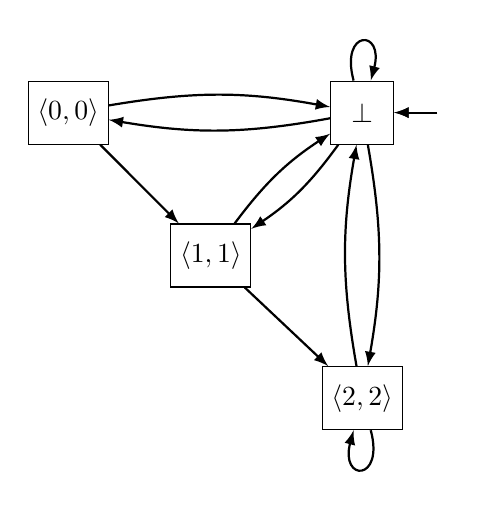
\begin{tikzpicture} [scale=1.2, every initial by arrow/.style={thick}]
%		\newcommand{\varstyle}[2]{\mt{\langle#1,#2\rangle}};
		
		\node [gstate,initial,initial right,initial text=](sbot) at (0,0) {\notppty};
		\node [gstate,left=80pt of sbot] (s00){\varstyle{0}{0}};
		\node [gstate,below left=of sbot] (s11) {\varstyle{1}{1}};
		\node [gstate,below=80pt of sbot] (s22) {\varstyle{2}{2}};			
		
		\path [trans] (s00) edge (s11);
		\path [trans] (s11) edge (s22);
		\path [bendtrans] (sbot) edge (s00);
		\path [bendtrans] (sbot) edge (s11);
		\path [bendtrans] (sbot) edge (s22);
		\path [bendtrans] (s00) edge (sbot);
		\path [bendtrans] (s11) edge (sbot);
		\path [bendtrans] (s22) edge (sbot);
		
		\path [trans] (s22) edge [loop below] (s22);
		\path [trans] (sbot) edge [loop above] (sbot);
		
		%		midway, at start, near start, very near start, at end, near end, very near end
		
		
	\end{tikzpicture}
\end{document}
	\end{minipage}
	\caption{Simplified representations of \mdp (left) and the \viewN \viewparamdnf on it (right)}
	\label{fig:varsDnf}  
\end{figure}

Analogously a view based on a conjunctive normal formal can be defined that may be more convenient, depending on the query.

\begin{definition}
	Let $\chgph = \chgphtuple$ be \achgphN and 
	\begin{align*}
		c(s) = &((\varstate[,i_1] \eqorneq \varval_{i_1}) \lor \dots \lor (\varstate[,i_{l_1}] \eqorneq \varval_{i_{l_1}})) \; \land \\
		&((\varstate[,i_{l_1+1}] \eqorneq \varval_{i_{l_1+1}}) \lor \dots \lor (\varstate[,i_{l_2}] \eqorneq \varval_{i_{l_2}})) \; \land  \\
		&\dots \\ 
		&((\varstate[,i_{(l_{m-1})+1}] \eqorneq \varval_{i_{(l_{m-1})+1}}) \lor \dots \lor (\varstate[,i_{l_m}]  \eqorneq \varval_{i_{l_m}}))
	\end{align*}
	
	proposition logical formula in disjunctive normal form where
	\begin{itemize}
			\item $\varstate[,i_k], a_{i_k} \in \varevalimg$ with $i_k\in \natnums$ and $k \in \{1, \dots, l_m\}$
			\item $l_1 < l_2 < \dots < l_m$ are natural numbers and $m$ is the number of clauses in $c(s)$
	\end{itemize}
	The \viewN \viewparamcnf is defined by its \grpfctN $\gfctparamcnf : \states \to \imggrp$ with
	\[
	\state \mapsto
	\begin{cases}
			\group, &\text{if } c(s) \text{ is true}\\
			\remelem, 	&\text{otherwise}
		\end{cases}
	\]
	
	where $\imggrp := \{\group, \remelem\}$.
\end{definition}

The only difference from the \viewN \viewparamcnf to the \viewN \viewparamdnf is whether the respective formulae is in conjunctive or disjunctive normal form.\redcomment{CITATION} Since each formulae in conjunctive normal form can tan be transformed to a formulae in disjunctive normal form and vice verse neither on of the \viewsN can perform an action the other can not. Hence there is no difference in expressivity, but there may be one in size. Therefore both views have been implemented and formalized. 

The views discussed before reduce the \chgphN in a very precise but also manual manner, because it not only dictates the variable but also its value. A more general approach is to stipulate only the variable but not its value. This way states will be grouped that have the same value for that variable with no regard to the actual value of that variable. This idea could be achieved with a view based on the \grpfctN $\grpfct[\varval_1 ]$%\pll \dots \pll \gfctparamvalueseqopt[\varval_n]]$ with $\redcomment{\vareval(\states, \var)} = \{\varval_1, \dots, \varval_n\}$ and $|\vareval(\states,\var)| = n$. This grouping function just groups on every possible value for the variable \var. Since this is \redcomment{not very practical} we define a view that achieves this result in a more direct and more efficient way.

\begin{definition}
	Let $\chgph = \chgphtuple$ be \achgphN. The view \viewparamvalident is defined by its \grpfctN $\gfctparamvalident : \states \to \imggrp$ with
	\[
	\state \mapsto \vareval(\state,\var)
	\]
	and $\imggrp := \vareval(\states, \var)$.
\end{definition}

With this grouping function we directly map to the value of the variable. Hence for $\state_1, \state_2 \in \states$ it is $\gfctparamvalident(\state_1) = \gfctparamvalident(\state_2)$ \iffN they are mapped to the value $\varval \in \imggrp$. Hence the equivalence classes of \eqrelview are
\[
\eqclassv[\smstate] = \{ \state \in \states \mid \vareval(\state) = \vareval(\smstate)\}.
\]
According to Definition \ref{def:view} the set $\states' := \bigcup_{\state \in \states} \eqclassv$ is the set of states of \viewparamvalident.

\begin{figure}[h]
	\begin{minipage}{.6\textwidth}
		%		\hspace{5mm}		
		\documentclass[tikz]{standalone}
%\usepackage{prelude}

%%%%%%%%%%%%%%%%%%%%%%%%%%%%%%%%%%%% PACKAGES %%%%%%%%%%%%%%%%%%%%%%%%%%%%%%%%%%%%%%%%%%

\usepackage{inputenc,fontenc}
\usepackage[a4paper,margin=3cm]{geometry}
\usepackage[english]{babel}
%\usepackage[german]{babel}
%\usepackage[fixlanguage]{babelbib}


\usepackage{bbold}
\usepackage{amsthm}
\usepackage{amsmath}
\usepackage{amssymb} % doteqdot
\usepackage[dvipsnames]{xcolor}
\usepackage{standalone}
\usepackage{tikz}[mode=buildnew]
\usepackage{cite}
\usepackage{xspace}
\usepackage{relsize}
\usepackage{mathtools} % mathclap
%\usepackage{MnSymbol}
\usepackage{hyperref}
\usepackage{url}
\usepackage{listings} % for code
\usepackage[T1]{fontenc} %<
\hypersetup{
	colorlinks,
	citecolor=black,
	filecolor=black,
	linkcolor=black,
	urlcolor=black
}
\usepackage{pgfplots}
\pgfplotsset{compat=1.18}
%\usepackage{courier} %% Sets font for listing as Courier. But also for url and texttt!
\usepackage{listings, xcolor}
\usepackage{graphicx}
\usepackage{subcaption}

\usetikzlibrary{calc}
%\usepackage{xparse} % \newDocumentCommand for multiple optional arguments
%\usepackage{titlecaps}



%%%%%%%%%%%%%%%%%%%%%%%%%%%%%%%%%%%% THEOREMSTYLES %%%%%%%%%%%%%%%%%%%%%%%%%%%%%%%%%%

\theoremstyle{definition}
\newtheorem{definition}{Definition}[section]
\newtheorem{exmp}{Beispiel}[section]
%\AfterEndEnvironment{definition}{\noindent\ignorespaces}

\theoremstyle{theorem}
\newtheorem{theorem}{Satz}[section]
\newtheorem{proposition}{Proposition}[section]
%\AfterEndEnvironment{theorem}{\noindent\ignorespaces}

\theoremstyle{korollary}
\newtheorem{korollary}{Korollar}[section]
%\AfterEndEnvironment{korollary}{\noindent\ignorespaces}


\tikzset{
	mstate/.style={draw, circle, minimum size=.94cm}, 
	gstate/.style={draw, rectangle, minimum size=.8cm},
	varstate/.style={draw,rectangle, rounded corners, minimum size=1}, 
	trans/.style={draw, ->, thick},
	bendtrans/.style={draw, ->, thick, bend left=10},
	bendtransr/.style={draw, ->, thick, bend right=10},
	init/.style={initial, initial distance=6pt, initial text=},
	every loop/.style={min distance=5pt, looseness=8},
	>=latex
}
\usetikzlibrary{automata,positioning}

%auto shift/.style={auto=right,->,
%	to path={ let \p1=(\tikztostart),\p2=(\tikztotarget),
%		\n1={atan2(\y2-\y1,\x2-\x1)},\n2={\n1+180}
%		in ($(\tikztostart.{\n1})!1mm!270:(\tikztotarget.{\n2})$) -- 
%		($(\tikztotarget.{\n2})!1mm!90:(\tikztostart.{\n1})$) \tikztonodes}},

%%%%%%%%%%%%%%%%%%%%%%%%%%%%%%%%%%% MY MACROS %%%%%%%%%%%%%%%%%%%%%%%%%%%%%%%%%%%%%%%%%
%formatting
\newcommand{\comment}[2]{{\color{#1}#2}}
\newcommand{\redcomment}[1]{{\color{red}#1}}
\newcommand{\purpcomment}[1]{{\color{pink}#1}}
\newcommand{\bluecomment}[1]{{\color{blue}#1}}
\newcommand{\mt}[1]{\ensuremath{{#1}}\xspace}
\newcommand{\mynewcommand}[2]{\newcommand{#1}{\mt{#2}}} %% currently not used becaue of ide highlighting
\newcommand{\arr}{\mt{\to}}

%model checking terms
\newcommand{\mimicrel}{\mt{\mathcal{R}}}
\newcommand{\bisimeq}{\mt{\;\!\sim\;\!}}
\newcommand{\simorder}{\mt{\;\!\preceq\;\!}}
\newcommand{\simequiv}{\mt{\;\!\simeq\;\!}} %command already defined
\newcommand{\relts}{\mt{\;\!\bullet_{_{\tiny{TS}}}\;\!}}
\newcommand{\rel}{\mt{\;\!\bullet\;\!}}

%own names
\newcommand{\nm}[1]{#1\xspace}
\newcommand{\mdpN}{\nm{MDP}}
\newcommand{\mdpsN}{\nm{MDPs}}
\newcommand{\viewN}{\nm{view}}
\newcommand{\viewNC}{\nm{View}}
\newcommand{\viewsN}{\nm{views}}
\newcommand{\viewsNC}{\nm{Views}}
\newcommand{\grpfctsubN}{\nm{detached grouping function}}
\newcommand{\grpfctsubNC}{\nm{detached grouping function}}
\newcommand{\grpfctsubNCC}{\nm{Detached Grouping Function}}
\newcommand{\grpfctN}{\nm{grouping function}}
\newcommand{\grpfctNC}{\nm{Grouping function}}
\newcommand{\grpfctNCC}{\nm{Grouping Function}}
\newcommand{\grpfctsN}{\nm{grouping functions}}
\newcommand{\grpfctsNC}{\nm{Grouping functions}}
\newcommand{\grpfctsNCC}{\nm{Grouping Functions}}
\newcommand{\stmimicN}{\nm{state-mimic}}
\newcommand{\stmimicsN}{\nm{state-mimics}}
\newcommand{\stmimickingN}{\nm{state-mimicking}}
\newcommand{\stmimickedN}{\nm{state-mimicked}}
%\newcommand{\chosenphtypeNCC}{\nm{Transition System}}
%\newcommand{\chgphNC}{\nm{Transition system}}
%\newcommand{\chgphN}{\nm{transition system}}
%\newcommand{\chgphsNCC}{\nm{Transition Systems}}
%\newcommand{\chgphsNC}{\nm{Transition systems}}
%\newcommand{\chgphsN}{\nm{transition systems}}
\newcommand{\chgphNCC}{\nm{MDP}}
\newcommand{\chgphNC}{\nm{MDP}}
\newcommand{\chgphN}{\nm{MDP}}
\newcommand{\achgphN}{\nm{an MDP}}
\newcommand{\chgphsNCC}{\nm{MDPs}}
\newcommand{\chgphsNC}{\nm{MDPs}}
\newcommand{\chgphsN}{\nm{MDPs}}
\newcommand{\parllcompN}{\nm{parallel composition}}
\newcommand{\parllcompNC}{\nm{Parallel composition}}
\newcommand{\parllcompNCC}{\nm{Parallel Composition}}
\newcommand{\parllcompsN}{\nm{parallel compositions}}
\newcommand{\parllcompsNC}{\nm{Parallel compositions}}
\newcommand{\parllcompsNCC}{\nm{Parallel Compositions}}
\newcommand{\sccN}{\nm{SCC}}
\newcommand{\sccsN}{\nm{SCCs}}
\newcommand{\bsccN}{\nm{BSCC}}
\newcommand{\bsccsN}{\nm{BSCCs}}
\newcommand{\jgrapht}{\nm{jGraphtT}}

\newcommand{\outactident}{\nm{OutActionsIdent}}

%names
\newcommand{\iffN}{\nm{if and only if}}
\newcommand{\tsN}{\nm{TS}}

%% outactions identical
\newcommand{\outactidentstrong}{\nm{strong}}
\newcommand{\outactidentweak}{\nm{weak}}

% CORE DEFINITIONS
\newcommand{\grpfct}[1][\viewppty]{\mt{F_{#1}}}
\newcommand{\grpfctsub}[1][\viewppty]{\mt{\tilde{F}_{#1}}}
%\newcommand{\grpfctimg}[1]{\mt{{\grpfct}[{#1}]}}
%\newcommand{\fctimg}[2]{\mt{{#1}[{#2}]}}
\newcommand{\eqrelview}{\mt{R}}
\newcommand{\eqclassv}[1][\state]{\mt{\eqclass{#1}{\eqrelview}}}
\newcommand{\eqclasssetv}[1][\states]{\mt{{#1}/\eqrelview}} %OLD: \bigcup_{\state \in \states} \eqclassv
\newcommand{\viewid}{\mt{\mdp}}
\newcommand{\view}[1][\viewppty]{\mt{\viewid_{#1}}}
\newcommand{\imggrp}{\mt{\arbset}}
\newcommand{\imggrpsub}{\mt{X}}
\newcommand{\viewppty}{\mt{\theta}}
\newcommand{\pll}{\mt{\;\!\pllpure\;\!}}
\newcommand{\pllrev}{\mt{\pllpure^{-1}}}
\newcommand{\pllpure}{\mt{||}}
\newcommand{\compselectset}{\mt{Z}}
\newcommand{\compselectpure}{\mt{\pllpure_\compselectset}}
\newcommand{\compselect}{\mt{\;\pllpure_\compselectset\;}}
\newcommand{\remstates}{\mt{\bigcup_{\state \in \states \setminus \states_1}\{\{\state\}\}}}
\newcommand{\nogroupstates}[1][\states_2]{\mt{\bigcup_{\state \in \states \setminus {#1}}\{\{\state\}\}}}
\newcommand{\remelem}{\mt{\bullet}}
\newcommand{\nogroupset}{\mt{\xi}}
\newcommand{\remset}{\mt{\{\remelem\}}}
\newcommand{\gfctpll}{\mt{\grpfct[\pll]}}
\newcommand{\group}{\mt{\top}}
\newcommand{\imggrpbinview}{\mt{\{\remelem, \notppty\}}}
\newcommand{\viewappset}{\mt{\tilde{\states}}}
\newcommand{\hasppty}{\mt{\top}}
\newcommand{\notppty}{\mt{\bot}}
\newcommand{\disregardelem}{\mt{\Delta}}
\newcommand{\disregardelements}{\mt{{\disregardelem_1, \dots, \disregardelem_n}}}



%\newcommand{\mdp}{def}\mdp
%\newcommand{\mdpdef}



% EXAMPLE VIEWS
\newcommand{\pptyatomicprops}{\mt{\atomicprops}}
\newcommand{\pptyinitstates}{\mt{\initstates}}
\newcommand{\pptyinactsetsize}{\mt{|\inacts(\state)|}}
\newcommand{\pptyhasoutact}{\mt{\exists\outact}}
\newcommand{\pptyminoutact}[2]{\mt{#1\leq#2}}
\newcommand{\pptymaxoutact}[2]{\mt{#2\leq#1}}
\newcommand{\pptyspanoutact}[3]{\mt{#1\leq#2\leq#3}}
\newcommand{\pptyoutactsetsize}{\mt{|\outacts(\state)|}}
\newcommand{\pptyoutactsingle}{\mt{|\outacts(\state)|_1}}
\newcommand{\pptystrongoutactident}{\mt{\outacts(\state)_=}}
\newcommand{\pptyweakoutactident}{\mt{\outacts(\state)_\approx}}
\newcommand{\pptyhasinact}{\mt{\exists\inact}}
\newcommand{\pptymininact}[2]{\mt{#1\leq#2}}
\newcommand{\pptymaxinact}[2]{\mt{#2\leq#1}}
\newcommand{\pptyspaninact}[3]{\mt{#1\leq#2\leq#3}}
\newcommand{\pptyinactsingle}{\mt{|\inacts(\state)|_1}}
\newcommand{\pptystronginactident}{\mt{\inacts(\state)_=}}
\newcommand{\pptyweakinactident}{\mt{\inacts(\state)_\approx}}
\newcommand{\pptyparamvalueseq}{\mt{\var = \varval}}
\newcommand{\pptyparamvaluesneq}{\mt{\var \neq \varval}}
\newcommand{\pptyparamdnf}{\mt{VarDNF}}
\newcommand{\pptyparamcnf}{\mt{VarCNF}}
\newcommand{\pptyparamvalueseqopt}{\mt{\var = \varval}}
\newcommand{\pptyparamvalident}{\mt{Var:\varval}}
\newcommand{\pptydistance}{\mt{\distpath}}
\newcommand{\pptydistancerev}{\mt{\distpathrev}}
\newcommand{\pptydistancebi}{\mt{\distpathbi}}
\newcommand{\pptyhascycle}{\mt{\exists\cycle}}
\newcommand{\pptyexactactcycle}{\mt{\{\cycle_{\action,n}\}}}
\newcommand{\pptycycleset}{\mt{\cup{\{\state\}_\cycle}}}
\newcommand{\pptyexactcycle}{\mt{\{\cycle_n\}}}
\newcommand{\pptyscc}{\mt{scc}}
\newcommand{\pptybscc}{\mt{bscc}}
\newcommand{\pptyprop}{\mt{\redcomment{?}}}
\newcommand{\pptyident}{id}


\newcommand{\gfctatomicprops}{\mt{\grpfct[\pptyatomicprops]}}
\newcommand{\gfctinitstates}{\mt{\grpfct[\pptyinitstates]^\hasppty}}
\newcommand{\gfcthasoutaction}{\mt{\grpfct[\pptyhasoutact]^\hasppty}}
\newcommand{\gfctminoutaction}{\mt{\grpfct[\pptyminoutact{\numoutact}{\outact}]^\hasppty}}
\newcommand{\gfctmaxoutaction}{\mt{\grpfct[\pptymaxoutact{\numoutact}{\outact}]^\hasppty}}
\newcommand{\gfctspanoutaction}{\mt{\grpfct[\pptyspanoutact{\numoutactb}{\outact}{\numoutact}]^\hasppty}}
\newcommand{\gfctoutactsetsize}{\mt{\grpfct[\pptyoutactsetsize]}}
\newcommand{\gfctoutactsingle}{\mt{\grpfct[\pptyoutactsingle]^\notppty}}
\newcommand{\gfctstrongoutactident}{\mt{\grpfct[\pptystrongoutactident]}}
\newcommand{\gfctweakoutactident}{\mt{\grpfct[\pptyweakoutactident]}}
\newcommand{\gfcthasinaction}{\mt{\grpfct[\pptyhasinact]^\hasppty}}
\newcommand{\gfctmininaction}{\mt{\grpfct[\pptymininact{\numinact}{\inact}]^\hasppty}}
\newcommand{\gfctmaxinaction}{\mt{\grpfct[\pptymaxinact{\numinact}{\inact}]^\hasppty}}
\newcommand{\gfctspaninaction}{\mt{\grpfct[\pptyspaninact{\numinactb}{\inact}{\numinact}]^\hasppty}}
\newcommand{\gfctinactsetsize}{\mt{\grpfct[\pptyinactsetsize]}}
\newcommand{\gfctinactsingle}{\mt{\grpfct[\pptyinactsingle]^\notppty}}
\newcommand{\gfctstronginactident}{\mt{\grpfct[\pptystronginactident]}}
\newcommand{\gfctweakinactident}{\mt{\grpfct[\pptyweakinactident]}}
\newcommand{\gfctparamvalueseq}{\mt{\grpfct[\pptyparamvalueseq]^\hasppty}}
\newcommand{\gfctparamvaluesneq}{\mt{\grpfct[\pptyparamvaluesneq]^\hasppty}}
\newcommand{\gfctparamdnf}{\mt{\grpfct[\pptyparamdnf]^\hasppty}}
\newcommand{\gfctparamcnf}{\mt{\grpfct[\pptyparamcnf]^\hasppty}}
\newcommand{\gfctparamvalueseqopt}{\mt{\pptyparamvalueseqopt}}
\newcommand{\gfctparamvalident}{\mt{\grpfct[\pptyparamvalident]}}
\newcommand{\gfctdistance}{\mt{\grpfct[\pptydistance]}}
\newcommand{\gfctdistancerev}{\mt{\grpfct[\pptydistancerev]}}
\newcommand{\gfctdistancebi}{\mt{\grpfct[\pptydistancebi]}}
\newcommand{\gfcthascycle}{\mt{\grpfct[\pptyhascycle]}}
\newcommand{\gfctexactcycle}{\mt{\grpfct[\pptyexactcycle]}}
\newcommand{\gfctcycleset}{\mt{\grpfct[\pptycycleset]}}
\newcommand{\gfctexactactcycle}{\mt{\grpfct[\pptyexactactcycle]}}
\newcommand{\gfctscc}{\mt{\grpfct[\pptyscc]}}
\newcommand{\gfctbscc}{\mt{\grpfct[\pptybscc]}}
\newcommand{\gfctprop}{\mt{\grpfct[\pptyprop]}}
\newcommand{\gfctident}{\mt{\grpfct[\pptyident]}}

\newcommand{\gfctsubatomicprops}{\mt{\grpfctsub[\pptyatomicprops]}}
\newcommand{\gfctsubinitstates}{\mt{\grpfctsub[\pptyinitstates]^\hasppty}}
\newcommand{\gfctsubhasoutaction}{\mt{\grpfctsub[\pptyhasoutact]^\hasppty}}
\newcommand{\gfctsubminoutaction}{\mt{\grpfctsub[\pptyminoutact{\numoutact}{\outact}]^\hasppty}}
\newcommand{\gfctsubmaxoutaction}{\mt{\grpfctsub[\pptymaxoutact{\numoutact}{\outact}]^\hasppty}}
\newcommand{\gfctsubspanoutaction}{\mt{\grpfctsub[\pptyspanoutact{\numoutactb}{\outact}{\numoutact}]^\hasppty}}
\newcommand{\gfctsuboutactsetsize}{\mt{\grpfctsub[\pptyoutactsetsize]}}
\newcommand{\gfctsuboutactsingle}{\mt{\grpfctsub[\pptyoutactsingle]^\notppty}}
\newcommand{\gfctsubstrongoutactident}{\mt{\grpfctsub[\pptystrongoutactident]^\hasppty}}
\newcommand{\gfctsubweakoutactident}{\mt{\grpfctsub[\pptyweakoutactident]^\hasppty}}
\newcommand{\gfctsubhasinaction}{\mt{\grpfctsub[\pptyhasinact]}}
\newcommand{\gfctsubmininaction}{\mt{\grpfctsub[\pptymininact{\numinact}{\inact}]}}
\newcommand{\gfctsubmaxinaction}{\mt{\grpfctsub[\pptymaxinact{\numinact}{\inact}]}}
\newcommand{\gfctsubspaninaction}{\mt{\grpfctsub[\pptyspaninact{\numinactb}{\inact}{\numinact}]}}
\newcommand{\gfctsubinactsetsize}{\mt{\grpfctsub[\pptyinactsetsize]^\hasppty}}
\newcommand{\gfctsubinactsingle}{\mt{\grpfctsub[\pptyinactsingle]^\notppty}}
\newcommand{\gfctsubstronginactident}{\mt{\grpfctsub[\pptystronginactident]}}
\newcommand{\gfctsubweakinactident}{\mt{\grpfctsub[\pptyweakinactident]}}
\newcommand{\gfctsubparamvalueseq}{\mt{\grpfctsub[\pptyparamvalueseq]^\hasppty}}
\newcommand{\gfctsubparamvaluesneq}{\mt{\grpfctsub[\pptyparamvaluesneq]^\hasppty}}
\newcommand{\gfctsubparamdnf}{\mt{\grpfctsub[\pptyparamdnf]^\hasppty}}
\newcommand{\gfctsubparamcnf}{\mt{\grpfctsub[\pptyparamcnf]^\hasppty}}
\newcommand{\gfctsubparamvalueseqopt}{\mt{\pptyparamvalueseqopt}}
\newcommand{\gfctsubparamvalident}{\mt{\grpfctsub[\pptyparamvalident]}}
\newcommand{\gfctsubdistance}{\mt{\grpfctsub[\pptydistance]}}
\newcommand{\gfctsubdistancerev}{\mt{\grpfctsub[\pptydistancerev]}}
\newcommand{\gfctsubdistancebi}{\mt{\grpfctsub[\pptydistancebi]}}
\newcommand{\gfctsubhascycle}{\mt{\grpfctsub[\pptyhascycle]^\hasppty}}
\newcommand{\gfctsubexactcycle}{\mt{\grpfctsub[\pptyexactcycle]}}
\newcommand{\gfctsubcycleset}{\mt{\grpfctsub[\pptycycleset]}}
\newcommand{\gfctsubexactactcycle}{\mt{\grpfctsub[\pptyexactactcycle]}}
\newcommand{\gfctsubscc}{\mt{\grpfctsub[\pptyscc]}}
\newcommand{\gfctsubbscc}{\mt{\grpfctsub[\pptybscc]}}
\newcommand{\gfctsubprop}{\mt{\grpfctsub[\pptyprop]}}
\newcommand{\gfctsubident}{\mt{\grpfctsub[\pptyident]}}


\newcommand{\viewatomicprops}{\mt{\view[\pptyatomicprops]}}
\newcommand{\viewinitstates}{\mt{\view[\pptyinitstates]^\hasppty}}
\newcommand{\viewhasoutaction}{\mt{\view[\pptyhasoutact]^\hasppty}}
\newcommand{\viewminoutaction}{\mt{\view[\pptyminoutact{\numoutact}{\outact}]^\hasppty}}
\newcommand{\viewmaxoutaction}{\mt{\view[\pptymaxoutact{\numoutact}{\outact}]^\hasppty}}
\newcommand{\viewspanoutaction}{\mt{\view[\pptyspanoutact{\numoutactb}{\outact}{\numoutact}]^\hasppty}}
\newcommand{\viewoutactsetsize}{\mt{\view[\pptyoutactsetsize]}}
\newcommand{\viewoutactsingle}{\mt{\view[\pptyoutactsingle]^\notppty}}
\newcommand{\viewstrongoutactident}{\mt{\view[\pptystrongoutactident]}}
\newcommand{\viewweakoutactident}{\mt{\view[\pptyweakoutactident]}}
\newcommand{\viewhasinaction}{\mt{\view[\pptyhasinact]^\hasppty}}
\newcommand{\viewmininaction}{\mt{\view[\pptymininact{\numinact}{\inact}]^\hasppty}}
\newcommand{\viewmaxinaction}{\mt{\view[\pptymaxinact{\numinact}{\inact}]^\hasppty}}
\newcommand{\viewspaninaction}{\mt{\view[\pptyspaninact{\numinactb}{\inact}{\numinact}]^\hasppty}}
\newcommand{\viewinactsetsize}{\mt{\view[\pptyinactsetsize]}}
\newcommand{\viewinactsingle}{\mt{\view[\pptyinactsingle]^\notppty}}
\newcommand{\viewstronginactident}{\mt{\view[\pptystronginactident]}}
\newcommand{\viewweakinactident}{\mt{\view[\pptyweakinactident]}}
\newcommand{\viewparamvalueseq}{\mt{\view[\pptyparamvalueseq]}}
\newcommand{\viewparamvaluesneq}{\mt{\view[\pptyparamvaluesneq]}}
\newcommand{\viewparamdnf}{\mt{\view[\pptyparamdnf]^\hasppty}}
\newcommand{\viewparamcnf}{\mt{\view[\pptyparamcnf]^\hasppty}}
\newcommand{\viewparamvalueseqopt}{\mt{\pptyparamvalueseqopt}}
\newcommand{\viewparamvalident}{\mt{\view[\pptyparamvalident]}}
\newcommand{\viewdistance}{\mt{\view[\pptydistance]}}
\newcommand{\viewdistancerev}{\mt{\view[\pptydistancerev]}}
\newcommand{\viewdistancebi}{\mt{\view[\pptydistancebi]}}
\newcommand{\viewhascycle}{\mt{\view[\pptyhascycle]}}
\newcommand{\viewexactcycle}{\mt{\view[\pptyexactcycle]}}
\newcommand{\viewcycleset}{\mt{\view[\pptycycleset]}}
\newcommand{\viewexactactcycle}{\mt{\view[\pptyexactactcycle]}}
\newcommand{\viewscc}{\mt{\view[\pptyscc]}}
\newcommand{\viewbscc}{\mt{\view[\pptybscc]}}
\newcommand{\viewprop}{\mt{\view[\pptyprop]}}
\newcommand{\viewident}{\mt{\view[\pptyident]}}

%\newcommand{\viewatomicprops}{\mt{\view[\atomicprops]}}
%\newcommand{\viewinitstates}{\mt{\view[\initstates]}}
%\newcommand{\viewhasoutaction}{\mt{\view[\pptyhasoutact]}}
%\newcommand{\viewminoutaction}{\mt{\view[\pptyminoutact{\numoutact}{\outact}]}}
%\newcommand{\viewmaxoutaction}{\mt{\view[\pptymaxoutact{\numoutact}{\outact}]}}
%\newcommand{\viewspanoutaction}{\mt{\view[\pptyspanoutact{\numoutactb}{\outact}{\numoutact}]}}
%\newcommand{\viewoutactsetsize}{\mt{\view[\pptyoutactsetsize]}}
%\newcommand{\viewoutactsingle}{\mt{\view[\pptyoutactsingle]}}
%\newcommand{\viewstrongoutactident}{\mt{\view[\outacts(\state)_=]}}
%\newcommand{\viewweakoutactident}{\mt{\view[\outacts(\state)_\approx]}}
%\newcommand{\viewhasinaction}{\mt{\view[\pptyhasinact]}}
%\newcommand{\viewmininaction}{\mt{\view[\pptymininact{\numinact}{\inact}]}}
%\newcommand{\viewmaxinaction}{\mt{\view[\pptymaxinact{\numinact}{\inact}]}}
%\newcommand{\viewspaninaction}{\mt{\view[\pptyspaninact{\numinactb}{\inact}{\numinact}]}}
%\newcommand{\viewinactsetsize}{\mt{\view[\pptyinactsetsize]}}
%\newcommand{\viewinactsingle}{\mt{\view[\pptyinactsingle]}}
%\newcommand{\viewstronginactident}{\mt{\view[\inacts(\state)_=]}}
%\newcommand{\viewweakinactident}{\mt{\view[\inacts(\state)_\approx]}}
%\newcommand{\viewparamvalueseq}{\mt{\view[\var = \varval]}}
%\newcommand{\viewparamvaluesneq}{\mt{\view[\var \neq \varval]}}
%\newcommand{\viewparamdnf}{\mt{\view[VarDNF]}}
%\newcommand{\viewparamcnf}{\mt{\view[VarCNF]}}
%\newcommand{\viewparamvalident}{\mt{\view[\pptyparamvalident]}}
%\newcommand{\viewdistance}{\mt{\view[\pptydistance]}}
%\newcommand{\viewhascycle}{\mt{\view[\exists\cycle]}}
%\newcommand{\viewexactcycle}{\mt{\view[\pptyexactcycle]}}
%\newcommand{\viewcycleset}{\mt{\view[\pptycycleset]}}
%\newcommand{\viewexactactcycle}{\mt{\view[\pptyexactactcycle]}}
%\newcommand{\viewscc}{\mt{\view[scc]}}
%\newcommand{\viewbscc}{\mt{\view[bscc]}}

%actions
\newcommand{\numoutact}{\mt{n}}
\newcommand{\numoutactb}{\mt{m}}
\newcommand{\numinact}{\mt{n}}
\newcommand{\numinactb}{\mt{m}}

\newcommand{\predmaxoutact}[1][\numoutact]{\mt{Q_{\outact\leq#1}(\state,\state_1, \dots, \state_{#1+1})}}
\newcommand{\predminoutact}[1][\numoutact]{\mt{Q_{#1\leq\outact}(\state,\state_1, \dots, \state_{#1})}}
\newcommand{\formoutact}[1][\state]{\mt{C_{#1,\outact}}}
\newcommand{\predmaxinact}[1][\numinact]{\mt{Q_{\inact\leq#1}(\state,\state_1, \dots, \state_{#1+1})}}
\newcommand{\predmininact}[1][\numinact]{\mt{Q_{#1\leq\inact}(\state,\state_1, \dots, \state_{#1})}}

\newcommand{\outact}[1][\action]{\mt{\overrightarrow{#1}}}
\newcommand{\outacts}{\mt{\overrightarrow{\actions}}}
\newcommand{\inact}{\mt{\overleftarrow{\action}}}
\newcommand{\inacts}[1][\action]{\mt{\overleftarrow{#1}}}

%%Parameters
\newcommand{\vars}[1][\mdp]{\mt{V\!ar_{#1}}}
\newcommand{\var}{\mt{x}}
\newcommand{\varstate}[1][]{\mt{\var_{\state#1}}}
\newcommand{\varval}{\mt{a}}
\newcommand{\vareval}[1][\mdp]{\mt{V\!arEval_{#1}}}
\newcommand{\varevalimg}[1][\mdp]{\mt{\vareval[#1][\states,\vars]}}
\newcommand{\varevalimgset}{\mt{\arbset}}
\newcommand{\someparam}{\mt{\tilde{x}}}
\newcommand{\eqorneq}{\mt{\;\doteqdot\;}}
\newcommand{\varstyle}[2]{\mt{\langle#1,#2\rangle}}




%\makeatletter
%\newcommand{\overleftrightsmallarrow}{\mathpalette{\overarrowsmall@\leftrightarrowfill@}}
%\newcommand{\overrightsmallarrow}{\mathpalette{\overarrowsmall@\rightarrowfill@}}
%\newcommand{\overleftsmallarrow}{\mathpalette{\overarrowsmall@\leftarrowfill@}}
%\newcommand{\overarrowsmall@}[3]{%
%	\vbox{%
%		\ialign{%
%			##\crcr
%			#1{\smaller@style{#2}}\crcr
%			\noalign{\nointerlineskip}%
%			$\m@th\hfil#2#3\hfil$\crcr
%		}%
%	}%
%}
%\def\smaller@style#1{%
%	\ifx#1\displaystyle\scriptstyle\else
%	\ifx#1\textstyle\scriptstyle\else
%	\scriptscriptstyle
%	\fi
%	\fi
%}
%\makeatother
%\newcommand{\te}[1]{\overleftrightsmallarrow{#1}}

% Distance
\newcommand{\fctdist}{\mt{distance}}
\newcommand{\fctdistdefault}{\mt{\fctdist(\chgph, \smstates, \grandist)}}
\newcommand{\distval}{\mt{d}}
\newcommand{\grandist}{\mt{n}}
\let\path\oldpath
\newcommand{\path}{\mt{P}}
\newcommand{\pathbi}{\mt{\bar{\path}}}
\newcommand{\pathsecfull}{\mt{(\state_0, \action_0, \state_1, \action_1, \dots, \action_{n}, \state_{n+1})}}
\newcommand{\lenpath}{\mt{len}}
\newcommand{\pfirst}{\mt{first}}
\newcommand{\plast}{\mt{last}}
\newcommand{\pathset}{\mt{\path_\chgph}}
\newcommand{\pathbiset}{\mt{\pathbi_\chgph}}
\newcommand{\distpath}{\mt{\overrightarrow{dist}}}
\newcommand{\distpathrev}{\mt{\overleftarrow{dist}}}
\newcommand{\distpathbi}{\mt{\overline{dist}}}
%Cycles
\newcommand{\cyclesecfull}{\mt{(\state_0, \action_0, \state_1, \action_1, \dots, \action_{n-1}, \state_0)}}
\newcommand{\fctfindcycles}{\mt{findCycles}}
\newcommand{\cycle}{\mt{C}}
\newcommand{\cycleset}{\mt{\cycle_{\mdp, n}}}
\newcommand{\lencycle}{\mt{len}}
% strongly connected components
\newcommand{\scc}{\mt{T}}
\newcommand{\setscc}{\mt{SCC_{\chgph,n}}}
\newcommand{\setbscc}{\mt{BSCC_{\chgph,n}}}

% properties
\newcommand{\propfct}{\mt{f}}

% all Systems
\newcommand{\chgph}{\mt{\mdp}}
\newcommand{\chgphtuple}{\mt{\mdptuple}}
\newcommand{\chgphtupledist}{\mt{\mdptupledist}}

\newcommand{\states}{\mt{S}}
\newcommand{\actions}{\mt{Act}}
\newcommand{\atomicprops}{\mt{AP}}
\newcommand{\labelingfct}{\mt{L}}
\newcommand{\init}{\mt{\initdistrib}} % use MDP % refers to the underlying set
\newcommand{\trans}{\mt{\probtfunc}} % use MDP % refers to the underlying set
\newcommand{\smstates}{\mt{\tilde{\states}}}


\newcommand{\state}{\mt{s}}
\newcommand{\action}{\mt{\alpha}}
\newcommand{\actionb}{\mt{\beta}}
\newcommand{\actionc}{\mt{\gamma}}
\newcommand{\smstate}{\mt{\tilde{\state}}}



% transition sysstems
\newcommand{\ts}{\mt{TS}}
\newcommand{\transitionrel}{\mt{\longrightarrow}}
\newcommand{\initstates}{\mt{I}}
\newcommand{\transitionsystem}{\mt
	{(\states, \actions, \transitionrel, \initstates, \atomicprops, \labelingfct)}
}
\newcommand{\tstupledist}{\mt{(\states', \actions',\transitionrel', \initstates', \labelingfct')}}


%Markov chains and MDP
\newcommand{\mdp}{\mt{\autm}}
\newcommand{\mdptuple}{\mt{(\states, \actions, \probtfunc, \initdistrib, \atomicprops, \labelingfct)}}
\newcommand{\mdptupledist}{\mt{(\states', \actions', \probtfunc', \initdistrib', \atomicprops', \labelingfct')}}
\newcommand{\autm}{\mt{\mathcal{M}}}
\newcommand{\probtfunc}{\mt{\textbf{P}}}
\newcommand{\initdistrib}{\mt{\iota_{init}}}


%maths
\newcommand{\powerset}[1]{\mt{\mathcal{P}(#1)}}
\newcommand{\eqclass}[2]{\mt{[#1]_{#2}}}%{\mt{#1 / #2}}
\newcommand{\impr}{\mt{\hspace{3mm}\Rightarrow\hspace{2mm}}}
\newcommand{\impl}{\mt{\hspace{3mm}\Leftarrow\hspace{2mm}}}
\newcommand{\natnums}{\mt{\mathbb{N}}} 
\newcommand{\realnums}{\mt{\mathbb{R}}}
\newcommand{\intmodn}[1][n]{\mt{\mathbb{Z}_{#1}}}
\newcommand{\arbset}{\mt{M}}
\newcommand{\bigsum}[2][]{\mt{\mathlarger{\sum}_{#2}^{#1}}}
\newcommand{\bbigsum}[2][]{\mt{\mathlarger{\mathlarger{\sum}}_{#2}^{#1}}}
\newcommand{\invimage}[2]{#1^{\mt{-1}(#2)}}
\newcommand{\img}{\mt{Img}}
\newcommand{\cond}{\mt{\,|\,}}

%tickz
%% \definecolor{darkred}{RGB}{196, 42, 42}

%implementation
\newcommand{\pmcvis}{\nm{PMC-Vis}}


\usepackage{tikz}
\newcommand{\stateppty}{draw, circle, minimum size=1cm}
\usepackage{ifthen}


\begin{document}
	\newcommand{\createstate}[3]{\node[draw, circle, minimum size=1cm] (#1) at (#2) {#3}}
	\newcommand{\basex}{0}
	\newcommand{\basey}{0}
	\begin{tikzpicture} [scale=2, every initial by arrow/.style={thick}]
		\newcommand{\varstyle}[2]{\mt{\langle#1,#2\rangle}};
		%		\createstate{s1}{3,2+4}{$\state_1$};

		\node [varstate,init] (s00) at (0,0){\varstyle{0}{0}};
		\node [varstate,right=of s00] (s01) {\varstyle{0}{1}};
		\node [varstate,right=of s01] (s02) {\varstyle{0}{2}};
		\node [varstate,below=of s00] (s10) {\varstyle{1}{0}};
		\node [varstate,right=of s10] (s11) {\varstyle{1}{1}};
		\node [varstate,right=of s11] (s12) {\varstyle{1}{2}};
		\node [varstate,below=of s10] (s20) {\varstyle{2}{0}};
		\node [varstate,right=of s20] (s21) {\varstyle{2}{1}};
		\node [varstate,right=of s21] (s22) {\varstyle{2}{2}};
		
%		\foreach \x in {0,...,2} 
%			\foreach \y [evaluate=\y as \i using \y+1] in {0,...,1}				
%				{	
%					\path [trans] (s\x\y) edge (s\x\i);
%					};
					
		\path [trans] (s00) edge (s01);
		\path [trans] (s01) edge (s02);
		\path [trans] (s10) edge (s11);
		\path [trans] (s11) edge (s12);
		\path [trans] (s20) edge (s21);
		\path [trans] (s21) edge (s22);
		\path [trans] (s00) edge (s10);
		\path [trans] (s10) edge (s20);
		\path [trans] (s01) edge (s11);
		\path [trans] (s11) edge (s21);
		\path [trans] (s02) edge (s12);
		\path [trans] (s12) edge (s22);
		
		\path [trans] (s22) edge [loop below] (s22);
				
%		\foreach \y in {0,...,2} 
%			\foreach \x in {0,...,1} 
%				{\path [trans] (s\x\y) edge (s\x+1\y);};
		
		
%		\foreach \x in {0,...,4} {
%			\foreach \y in {\x,...,4} {
%				\x --["\ifthenelse{\x=3 \OR \y=3 \OR \x=\y}{}{\x\y}",sloped] \y;
%				}}};
		
		
		%		\node [mstate,below right=40pt and 30 pt of s2] (s5) {$\state_5$};
%		\node [mstate,below=of s3] (s6) {$\state_6$};
%		\node [mstate,right=55pt of s6] (s7) {$\state_7$};
%		\node [mstate,below left=20pt and 30pt of s1] (s8) {$\state_8$};
%		\node [mstate,below=20pt of s8] (s9) {$\state_9$};
%		%		\node [mstate,right=of s2] (s10) {$\state_{10}$};
%		\node [mstate,above=26pt of s5] (s10) {$\state_{10}$};
%		
%		
%		
%		\path [trans] (s1) edge (s2);
%		\path [trans] (s1) edge (s3);
%		\path [trans] (s1) edge (s3);
%		\path [trans] (s1) edge (s8);
%		\path [trans] (s2) edge (s4);
%		\path [trans] (s3) edge (s4);
%		\path [trans] (s3) edge (s6);
%		\path [trans] (s5) edge (s2);
%		\path [trans] (s5) edge (s6);
%		\path [trans] (s5) edge (s7);
%		\path [trans] (s6) edge (s7);
%		\path [trans] (s9) edge (s8);
%		\path [trans] (s9) edge (s6);
%		
%		\path [trans] (s2) edge [loop above] (s2);
%		\path [trans] (s7) edge [loop right] (s7);
%		\path [trans] (s9) edge [loop below] (s9);
%		
	\end{tikzpicture}
\end{document}
	\end{minipage}%
	\begin{minipage}{.5\textwidth}
		\documentclass[tikz,preview]{standalone}
%\usepackage{prelude}

%%%%%%%%%%%%%%%%%%%%%%%%%%%%%%%%%%%% PACKAGES %%%%%%%%%%%%%%%%%%%%%%%%%%%%%%%%%%%%%%%%%%

\usepackage{inputenc,fontenc}
\usepackage[a4paper,margin=3cm]{geometry}
\usepackage[english]{babel}
%\usepackage[german]{babel}
%\usepackage[fixlanguage]{babelbib}


\usepackage{bbold}
\usepackage{amsthm}
\usepackage{amsmath}
\usepackage{amssymb} % doteqdot
\usepackage[dvipsnames]{xcolor}
\usepackage{standalone}
\usepackage{tikz}[mode=buildnew]
\usepackage{cite}
\usepackage{xspace}
\usepackage{relsize}
\usepackage{mathtools} % mathclap
%\usepackage{MnSymbol}
\usepackage{hyperref}
\usepackage{url}
\usepackage{listings} % for code
\usepackage[T1]{fontenc} %<
\hypersetup{
	colorlinks,
	citecolor=black,
	filecolor=black,
	linkcolor=black,
	urlcolor=black
}
\usepackage{pgfplots}
\pgfplotsset{compat=1.18}
%\usepackage{courier} %% Sets font for listing as Courier. But also for url and texttt!
\usepackage{listings, xcolor}
\usepackage{graphicx}
\usepackage{subcaption}

\usetikzlibrary{calc}
%\usepackage{xparse} % \newDocumentCommand for multiple optional arguments
%\usepackage{titlecaps}



%%%%%%%%%%%%%%%%%%%%%%%%%%%%%%%%%%%% THEOREMSTYLES %%%%%%%%%%%%%%%%%%%%%%%%%%%%%%%%%%

\theoremstyle{definition}
\newtheorem{definition}{Definition}[section]
\newtheorem{exmp}{Beispiel}[section]
%\AfterEndEnvironment{definition}{\noindent\ignorespaces}

\theoremstyle{theorem}
\newtheorem{theorem}{Satz}[section]
\newtheorem{proposition}{Proposition}[section]
%\AfterEndEnvironment{theorem}{\noindent\ignorespaces}

\theoremstyle{korollary}
\newtheorem{korollary}{Korollar}[section]
%\AfterEndEnvironment{korollary}{\noindent\ignorespaces}


\tikzset{
	mstate/.style={draw, circle, minimum size=.94cm}, 
	gstate/.style={draw, rectangle, minimum size=.8cm},
	varstate/.style={draw,rectangle, rounded corners, minimum size=1}, 
	trans/.style={draw, ->, thick},
	bendtrans/.style={draw, ->, thick, bend left=10},
	bendtransr/.style={draw, ->, thick, bend right=10},
	init/.style={initial, initial distance=6pt, initial text=},
	every loop/.style={min distance=5pt, looseness=8},
	>=latex
}
\usetikzlibrary{automata,positioning}

%auto shift/.style={auto=right,->,
%	to path={ let \p1=(\tikztostart),\p2=(\tikztotarget),
%		\n1={atan2(\y2-\y1,\x2-\x1)},\n2={\n1+180}
%		in ($(\tikztostart.{\n1})!1mm!270:(\tikztotarget.{\n2})$) -- 
%		($(\tikztotarget.{\n2})!1mm!90:(\tikztostart.{\n1})$) \tikztonodes}},

%%%%%%%%%%%%%%%%%%%%%%%%%%%%%%%%%%% MY MACROS %%%%%%%%%%%%%%%%%%%%%%%%%%%%%%%%%%%%%%%%%
%formatting
\newcommand{\comment}[2]{{\color{#1}#2}}
\newcommand{\redcomment}[1]{{\color{red}#1}}
\newcommand{\purpcomment}[1]{{\color{pink}#1}}
\newcommand{\bluecomment}[1]{{\color{blue}#1}}
\newcommand{\mt}[1]{\ensuremath{{#1}}\xspace}
\newcommand{\mynewcommand}[2]{\newcommand{#1}{\mt{#2}}} %% currently not used becaue of ide highlighting
\newcommand{\arr}{\mt{\to}}

%model checking terms
\newcommand{\mimicrel}{\mt{\mathcal{R}}}
\newcommand{\bisimeq}{\mt{\;\!\sim\;\!}}
\newcommand{\simorder}{\mt{\;\!\preceq\;\!}}
\newcommand{\simequiv}{\mt{\;\!\simeq\;\!}} %command already defined
\newcommand{\relts}{\mt{\;\!\bullet_{_{\tiny{TS}}}\;\!}}
\newcommand{\rel}{\mt{\;\!\bullet\;\!}}

%own names
\newcommand{\nm}[1]{#1\xspace}
\newcommand{\mdpN}{\nm{MDP}}
\newcommand{\mdpsN}{\nm{MDPs}}
\newcommand{\viewN}{\nm{view}}
\newcommand{\viewNC}{\nm{View}}
\newcommand{\viewsN}{\nm{views}}
\newcommand{\viewsNC}{\nm{Views}}
\newcommand{\grpfctsubN}{\nm{detached grouping function}}
\newcommand{\grpfctsubNC}{\nm{detached grouping function}}
\newcommand{\grpfctsubNCC}{\nm{Detached Grouping Function}}
\newcommand{\grpfctN}{\nm{grouping function}}
\newcommand{\grpfctNC}{\nm{Grouping function}}
\newcommand{\grpfctNCC}{\nm{Grouping Function}}
\newcommand{\grpfctsN}{\nm{grouping functions}}
\newcommand{\grpfctsNC}{\nm{Grouping functions}}
\newcommand{\grpfctsNCC}{\nm{Grouping Functions}}
\newcommand{\stmimicN}{\nm{state-mimic}}
\newcommand{\stmimicsN}{\nm{state-mimics}}
\newcommand{\stmimickingN}{\nm{state-mimicking}}
\newcommand{\stmimickedN}{\nm{state-mimicked}}
%\newcommand{\chosenphtypeNCC}{\nm{Transition System}}
%\newcommand{\chgphNC}{\nm{Transition system}}
%\newcommand{\chgphN}{\nm{transition system}}
%\newcommand{\chgphsNCC}{\nm{Transition Systems}}
%\newcommand{\chgphsNC}{\nm{Transition systems}}
%\newcommand{\chgphsN}{\nm{transition systems}}
\newcommand{\chgphNCC}{\nm{MDP}}
\newcommand{\chgphNC}{\nm{MDP}}
\newcommand{\chgphN}{\nm{MDP}}
\newcommand{\achgphN}{\nm{an MDP}}
\newcommand{\chgphsNCC}{\nm{MDPs}}
\newcommand{\chgphsNC}{\nm{MDPs}}
\newcommand{\chgphsN}{\nm{MDPs}}
\newcommand{\parllcompN}{\nm{parallel composition}}
\newcommand{\parllcompNC}{\nm{Parallel composition}}
\newcommand{\parllcompNCC}{\nm{Parallel Composition}}
\newcommand{\parllcompsN}{\nm{parallel compositions}}
\newcommand{\parllcompsNC}{\nm{Parallel compositions}}
\newcommand{\parllcompsNCC}{\nm{Parallel Compositions}}
\newcommand{\sccN}{\nm{SCC}}
\newcommand{\sccsN}{\nm{SCCs}}
\newcommand{\bsccN}{\nm{BSCC}}
\newcommand{\bsccsN}{\nm{BSCCs}}
\newcommand{\jgrapht}{\nm{jGraphtT}}

\newcommand{\outactident}{\nm{OutActionsIdent}}

%names
\newcommand{\iffN}{\nm{if and only if}}
\newcommand{\tsN}{\nm{TS}}

%% outactions identical
\newcommand{\outactidentstrong}{\nm{strong}}
\newcommand{\outactidentweak}{\nm{weak}}

% CORE DEFINITIONS
\newcommand{\grpfct}[1][\viewppty]{\mt{F_{#1}}}
\newcommand{\grpfctsub}[1][\viewppty]{\mt{\tilde{F}_{#1}}}
%\newcommand{\grpfctimg}[1]{\mt{{\grpfct}[{#1}]}}
%\newcommand{\fctimg}[2]{\mt{{#1}[{#2}]}}
\newcommand{\eqrelview}{\mt{R}}
\newcommand{\eqclassv}[1][\state]{\mt{\eqclass{#1}{\eqrelview}}}
\newcommand{\eqclasssetv}[1][\states]{\mt{{#1}/\eqrelview}} %OLD: \bigcup_{\state \in \states} \eqclassv
\newcommand{\viewid}{\mt{\mdp}}
\newcommand{\view}[1][\viewppty]{\mt{\viewid_{#1}}}
\newcommand{\imggrp}{\mt{\arbset}}
\newcommand{\imggrpsub}{\mt{X}}
\newcommand{\viewppty}{\mt{\theta}}
\newcommand{\pll}{\mt{\;\!\pllpure\;\!}}
\newcommand{\pllrev}{\mt{\pllpure^{-1}}}
\newcommand{\pllpure}{\mt{||}}
\newcommand{\compselectset}{\mt{Z}}
\newcommand{\compselectpure}{\mt{\pllpure_\compselectset}}
\newcommand{\compselect}{\mt{\;\pllpure_\compselectset\;}}
\newcommand{\remstates}{\mt{\bigcup_{\state \in \states \setminus \states_1}\{\{\state\}\}}}
\newcommand{\nogroupstates}[1][\states_2]{\mt{\bigcup_{\state \in \states \setminus {#1}}\{\{\state\}\}}}
\newcommand{\remelem}{\mt{\bullet}}
\newcommand{\nogroupset}{\mt{\xi}}
\newcommand{\remset}{\mt{\{\remelem\}}}
\newcommand{\gfctpll}{\mt{\grpfct[\pll]}}
\newcommand{\group}{\mt{\top}}
\newcommand{\imggrpbinview}{\mt{\{\remelem, \notppty\}}}
\newcommand{\viewappset}{\mt{\tilde{\states}}}
\newcommand{\hasppty}{\mt{\top}}
\newcommand{\notppty}{\mt{\bot}}
\newcommand{\disregardelem}{\mt{\Delta}}
\newcommand{\disregardelements}{\mt{{\disregardelem_1, \dots, \disregardelem_n}}}



%\newcommand{\mdp}{def}\mdp
%\newcommand{\mdpdef}



% EXAMPLE VIEWS
\newcommand{\pptyatomicprops}{\mt{\atomicprops}}
\newcommand{\pptyinitstates}{\mt{\initstates}}
\newcommand{\pptyinactsetsize}{\mt{|\inacts(\state)|}}
\newcommand{\pptyhasoutact}{\mt{\exists\outact}}
\newcommand{\pptyminoutact}[2]{\mt{#1\leq#2}}
\newcommand{\pptymaxoutact}[2]{\mt{#2\leq#1}}
\newcommand{\pptyspanoutact}[3]{\mt{#1\leq#2\leq#3}}
\newcommand{\pptyoutactsetsize}{\mt{|\outacts(\state)|}}
\newcommand{\pptyoutactsingle}{\mt{|\outacts(\state)|_1}}
\newcommand{\pptystrongoutactident}{\mt{\outacts(\state)_=}}
\newcommand{\pptyweakoutactident}{\mt{\outacts(\state)_\approx}}
\newcommand{\pptyhasinact}{\mt{\exists\inact}}
\newcommand{\pptymininact}[2]{\mt{#1\leq#2}}
\newcommand{\pptymaxinact}[2]{\mt{#2\leq#1}}
\newcommand{\pptyspaninact}[3]{\mt{#1\leq#2\leq#3}}
\newcommand{\pptyinactsingle}{\mt{|\inacts(\state)|_1}}
\newcommand{\pptystronginactident}{\mt{\inacts(\state)_=}}
\newcommand{\pptyweakinactident}{\mt{\inacts(\state)_\approx}}
\newcommand{\pptyparamvalueseq}{\mt{\var = \varval}}
\newcommand{\pptyparamvaluesneq}{\mt{\var \neq \varval}}
\newcommand{\pptyparamdnf}{\mt{VarDNF}}
\newcommand{\pptyparamcnf}{\mt{VarCNF}}
\newcommand{\pptyparamvalueseqopt}{\mt{\var = \varval}}
\newcommand{\pptyparamvalident}{\mt{Var:\varval}}
\newcommand{\pptydistance}{\mt{\distpath}}
\newcommand{\pptydistancerev}{\mt{\distpathrev}}
\newcommand{\pptydistancebi}{\mt{\distpathbi}}
\newcommand{\pptyhascycle}{\mt{\exists\cycle}}
\newcommand{\pptyexactactcycle}{\mt{\{\cycle_{\action,n}\}}}
\newcommand{\pptycycleset}{\mt{\cup{\{\state\}_\cycle}}}
\newcommand{\pptyexactcycle}{\mt{\{\cycle_n\}}}
\newcommand{\pptyscc}{\mt{scc}}
\newcommand{\pptybscc}{\mt{bscc}}
\newcommand{\pptyprop}{\mt{\redcomment{?}}}
\newcommand{\pptyident}{id}


\newcommand{\gfctatomicprops}{\mt{\grpfct[\pptyatomicprops]}}
\newcommand{\gfctinitstates}{\mt{\grpfct[\pptyinitstates]^\hasppty}}
\newcommand{\gfcthasoutaction}{\mt{\grpfct[\pptyhasoutact]^\hasppty}}
\newcommand{\gfctminoutaction}{\mt{\grpfct[\pptyminoutact{\numoutact}{\outact}]^\hasppty}}
\newcommand{\gfctmaxoutaction}{\mt{\grpfct[\pptymaxoutact{\numoutact}{\outact}]^\hasppty}}
\newcommand{\gfctspanoutaction}{\mt{\grpfct[\pptyspanoutact{\numoutactb}{\outact}{\numoutact}]^\hasppty}}
\newcommand{\gfctoutactsetsize}{\mt{\grpfct[\pptyoutactsetsize]}}
\newcommand{\gfctoutactsingle}{\mt{\grpfct[\pptyoutactsingle]^\notppty}}
\newcommand{\gfctstrongoutactident}{\mt{\grpfct[\pptystrongoutactident]}}
\newcommand{\gfctweakoutactident}{\mt{\grpfct[\pptyweakoutactident]}}
\newcommand{\gfcthasinaction}{\mt{\grpfct[\pptyhasinact]^\hasppty}}
\newcommand{\gfctmininaction}{\mt{\grpfct[\pptymininact{\numinact}{\inact}]^\hasppty}}
\newcommand{\gfctmaxinaction}{\mt{\grpfct[\pptymaxinact{\numinact}{\inact}]^\hasppty}}
\newcommand{\gfctspaninaction}{\mt{\grpfct[\pptyspaninact{\numinactb}{\inact}{\numinact}]^\hasppty}}
\newcommand{\gfctinactsetsize}{\mt{\grpfct[\pptyinactsetsize]}}
\newcommand{\gfctinactsingle}{\mt{\grpfct[\pptyinactsingle]^\notppty}}
\newcommand{\gfctstronginactident}{\mt{\grpfct[\pptystronginactident]}}
\newcommand{\gfctweakinactident}{\mt{\grpfct[\pptyweakinactident]}}
\newcommand{\gfctparamvalueseq}{\mt{\grpfct[\pptyparamvalueseq]^\hasppty}}
\newcommand{\gfctparamvaluesneq}{\mt{\grpfct[\pptyparamvaluesneq]^\hasppty}}
\newcommand{\gfctparamdnf}{\mt{\grpfct[\pptyparamdnf]^\hasppty}}
\newcommand{\gfctparamcnf}{\mt{\grpfct[\pptyparamcnf]^\hasppty}}
\newcommand{\gfctparamvalueseqopt}{\mt{\pptyparamvalueseqopt}}
\newcommand{\gfctparamvalident}{\mt{\grpfct[\pptyparamvalident]}}
\newcommand{\gfctdistance}{\mt{\grpfct[\pptydistance]}}
\newcommand{\gfctdistancerev}{\mt{\grpfct[\pptydistancerev]}}
\newcommand{\gfctdistancebi}{\mt{\grpfct[\pptydistancebi]}}
\newcommand{\gfcthascycle}{\mt{\grpfct[\pptyhascycle]}}
\newcommand{\gfctexactcycle}{\mt{\grpfct[\pptyexactcycle]}}
\newcommand{\gfctcycleset}{\mt{\grpfct[\pptycycleset]}}
\newcommand{\gfctexactactcycle}{\mt{\grpfct[\pptyexactactcycle]}}
\newcommand{\gfctscc}{\mt{\grpfct[\pptyscc]}}
\newcommand{\gfctbscc}{\mt{\grpfct[\pptybscc]}}
\newcommand{\gfctprop}{\mt{\grpfct[\pptyprop]}}
\newcommand{\gfctident}{\mt{\grpfct[\pptyident]}}

\newcommand{\gfctsubatomicprops}{\mt{\grpfctsub[\pptyatomicprops]}}
\newcommand{\gfctsubinitstates}{\mt{\grpfctsub[\pptyinitstates]^\hasppty}}
\newcommand{\gfctsubhasoutaction}{\mt{\grpfctsub[\pptyhasoutact]^\hasppty}}
\newcommand{\gfctsubminoutaction}{\mt{\grpfctsub[\pptyminoutact{\numoutact}{\outact}]^\hasppty}}
\newcommand{\gfctsubmaxoutaction}{\mt{\grpfctsub[\pptymaxoutact{\numoutact}{\outact}]^\hasppty}}
\newcommand{\gfctsubspanoutaction}{\mt{\grpfctsub[\pptyspanoutact{\numoutactb}{\outact}{\numoutact}]^\hasppty}}
\newcommand{\gfctsuboutactsetsize}{\mt{\grpfctsub[\pptyoutactsetsize]}}
\newcommand{\gfctsuboutactsingle}{\mt{\grpfctsub[\pptyoutactsingle]^\notppty}}
\newcommand{\gfctsubstrongoutactident}{\mt{\grpfctsub[\pptystrongoutactident]^\hasppty}}
\newcommand{\gfctsubweakoutactident}{\mt{\grpfctsub[\pptyweakoutactident]^\hasppty}}
\newcommand{\gfctsubhasinaction}{\mt{\grpfctsub[\pptyhasinact]}}
\newcommand{\gfctsubmininaction}{\mt{\grpfctsub[\pptymininact{\numinact}{\inact}]}}
\newcommand{\gfctsubmaxinaction}{\mt{\grpfctsub[\pptymaxinact{\numinact}{\inact}]}}
\newcommand{\gfctsubspaninaction}{\mt{\grpfctsub[\pptyspaninact{\numinactb}{\inact}{\numinact}]}}
\newcommand{\gfctsubinactsetsize}{\mt{\grpfctsub[\pptyinactsetsize]^\hasppty}}
\newcommand{\gfctsubinactsingle}{\mt{\grpfctsub[\pptyinactsingle]^\notppty}}
\newcommand{\gfctsubstronginactident}{\mt{\grpfctsub[\pptystronginactident]}}
\newcommand{\gfctsubweakinactident}{\mt{\grpfctsub[\pptyweakinactident]}}
\newcommand{\gfctsubparamvalueseq}{\mt{\grpfctsub[\pptyparamvalueseq]^\hasppty}}
\newcommand{\gfctsubparamvaluesneq}{\mt{\grpfctsub[\pptyparamvaluesneq]^\hasppty}}
\newcommand{\gfctsubparamdnf}{\mt{\grpfctsub[\pptyparamdnf]^\hasppty}}
\newcommand{\gfctsubparamcnf}{\mt{\grpfctsub[\pptyparamcnf]^\hasppty}}
\newcommand{\gfctsubparamvalueseqopt}{\mt{\pptyparamvalueseqopt}}
\newcommand{\gfctsubparamvalident}{\mt{\grpfctsub[\pptyparamvalident]}}
\newcommand{\gfctsubdistance}{\mt{\grpfctsub[\pptydistance]}}
\newcommand{\gfctsubdistancerev}{\mt{\grpfctsub[\pptydistancerev]}}
\newcommand{\gfctsubdistancebi}{\mt{\grpfctsub[\pptydistancebi]}}
\newcommand{\gfctsubhascycle}{\mt{\grpfctsub[\pptyhascycle]^\hasppty}}
\newcommand{\gfctsubexactcycle}{\mt{\grpfctsub[\pptyexactcycle]}}
\newcommand{\gfctsubcycleset}{\mt{\grpfctsub[\pptycycleset]}}
\newcommand{\gfctsubexactactcycle}{\mt{\grpfctsub[\pptyexactactcycle]}}
\newcommand{\gfctsubscc}{\mt{\grpfctsub[\pptyscc]}}
\newcommand{\gfctsubbscc}{\mt{\grpfctsub[\pptybscc]}}
\newcommand{\gfctsubprop}{\mt{\grpfctsub[\pptyprop]}}
\newcommand{\gfctsubident}{\mt{\grpfctsub[\pptyident]}}


\newcommand{\viewatomicprops}{\mt{\view[\pptyatomicprops]}}
\newcommand{\viewinitstates}{\mt{\view[\pptyinitstates]^\hasppty}}
\newcommand{\viewhasoutaction}{\mt{\view[\pptyhasoutact]^\hasppty}}
\newcommand{\viewminoutaction}{\mt{\view[\pptyminoutact{\numoutact}{\outact}]^\hasppty}}
\newcommand{\viewmaxoutaction}{\mt{\view[\pptymaxoutact{\numoutact}{\outact}]^\hasppty}}
\newcommand{\viewspanoutaction}{\mt{\view[\pptyspanoutact{\numoutactb}{\outact}{\numoutact}]^\hasppty}}
\newcommand{\viewoutactsetsize}{\mt{\view[\pptyoutactsetsize]}}
\newcommand{\viewoutactsingle}{\mt{\view[\pptyoutactsingle]^\notppty}}
\newcommand{\viewstrongoutactident}{\mt{\view[\pptystrongoutactident]}}
\newcommand{\viewweakoutactident}{\mt{\view[\pptyweakoutactident]}}
\newcommand{\viewhasinaction}{\mt{\view[\pptyhasinact]^\hasppty}}
\newcommand{\viewmininaction}{\mt{\view[\pptymininact{\numinact}{\inact}]^\hasppty}}
\newcommand{\viewmaxinaction}{\mt{\view[\pptymaxinact{\numinact}{\inact}]^\hasppty}}
\newcommand{\viewspaninaction}{\mt{\view[\pptyspaninact{\numinactb}{\inact}{\numinact}]^\hasppty}}
\newcommand{\viewinactsetsize}{\mt{\view[\pptyinactsetsize]}}
\newcommand{\viewinactsingle}{\mt{\view[\pptyinactsingle]^\notppty}}
\newcommand{\viewstronginactident}{\mt{\view[\pptystronginactident]}}
\newcommand{\viewweakinactident}{\mt{\view[\pptyweakinactident]}}
\newcommand{\viewparamvalueseq}{\mt{\view[\pptyparamvalueseq]}}
\newcommand{\viewparamvaluesneq}{\mt{\view[\pptyparamvaluesneq]}}
\newcommand{\viewparamdnf}{\mt{\view[\pptyparamdnf]^\hasppty}}
\newcommand{\viewparamcnf}{\mt{\view[\pptyparamcnf]^\hasppty}}
\newcommand{\viewparamvalueseqopt}{\mt{\pptyparamvalueseqopt}}
\newcommand{\viewparamvalident}{\mt{\view[\pptyparamvalident]}}
\newcommand{\viewdistance}{\mt{\view[\pptydistance]}}
\newcommand{\viewdistancerev}{\mt{\view[\pptydistancerev]}}
\newcommand{\viewdistancebi}{\mt{\view[\pptydistancebi]}}
\newcommand{\viewhascycle}{\mt{\view[\pptyhascycle]}}
\newcommand{\viewexactcycle}{\mt{\view[\pptyexactcycle]}}
\newcommand{\viewcycleset}{\mt{\view[\pptycycleset]}}
\newcommand{\viewexactactcycle}{\mt{\view[\pptyexactactcycle]}}
\newcommand{\viewscc}{\mt{\view[\pptyscc]}}
\newcommand{\viewbscc}{\mt{\view[\pptybscc]}}
\newcommand{\viewprop}{\mt{\view[\pptyprop]}}
\newcommand{\viewident}{\mt{\view[\pptyident]}}

%\newcommand{\viewatomicprops}{\mt{\view[\atomicprops]}}
%\newcommand{\viewinitstates}{\mt{\view[\initstates]}}
%\newcommand{\viewhasoutaction}{\mt{\view[\pptyhasoutact]}}
%\newcommand{\viewminoutaction}{\mt{\view[\pptyminoutact{\numoutact}{\outact}]}}
%\newcommand{\viewmaxoutaction}{\mt{\view[\pptymaxoutact{\numoutact}{\outact}]}}
%\newcommand{\viewspanoutaction}{\mt{\view[\pptyspanoutact{\numoutactb}{\outact}{\numoutact}]}}
%\newcommand{\viewoutactsetsize}{\mt{\view[\pptyoutactsetsize]}}
%\newcommand{\viewoutactsingle}{\mt{\view[\pptyoutactsingle]}}
%\newcommand{\viewstrongoutactident}{\mt{\view[\outacts(\state)_=]}}
%\newcommand{\viewweakoutactident}{\mt{\view[\outacts(\state)_\approx]}}
%\newcommand{\viewhasinaction}{\mt{\view[\pptyhasinact]}}
%\newcommand{\viewmininaction}{\mt{\view[\pptymininact{\numinact}{\inact}]}}
%\newcommand{\viewmaxinaction}{\mt{\view[\pptymaxinact{\numinact}{\inact}]}}
%\newcommand{\viewspaninaction}{\mt{\view[\pptyspaninact{\numinactb}{\inact}{\numinact}]}}
%\newcommand{\viewinactsetsize}{\mt{\view[\pptyinactsetsize]}}
%\newcommand{\viewinactsingle}{\mt{\view[\pptyinactsingle]}}
%\newcommand{\viewstronginactident}{\mt{\view[\inacts(\state)_=]}}
%\newcommand{\viewweakinactident}{\mt{\view[\inacts(\state)_\approx]}}
%\newcommand{\viewparamvalueseq}{\mt{\view[\var = \varval]}}
%\newcommand{\viewparamvaluesneq}{\mt{\view[\var \neq \varval]}}
%\newcommand{\viewparamdnf}{\mt{\view[VarDNF]}}
%\newcommand{\viewparamcnf}{\mt{\view[VarCNF]}}
%\newcommand{\viewparamvalident}{\mt{\view[\pptyparamvalident]}}
%\newcommand{\viewdistance}{\mt{\view[\pptydistance]}}
%\newcommand{\viewhascycle}{\mt{\view[\exists\cycle]}}
%\newcommand{\viewexactcycle}{\mt{\view[\pptyexactcycle]}}
%\newcommand{\viewcycleset}{\mt{\view[\pptycycleset]}}
%\newcommand{\viewexactactcycle}{\mt{\view[\pptyexactactcycle]}}
%\newcommand{\viewscc}{\mt{\view[scc]}}
%\newcommand{\viewbscc}{\mt{\view[bscc]}}

%actions
\newcommand{\numoutact}{\mt{n}}
\newcommand{\numoutactb}{\mt{m}}
\newcommand{\numinact}{\mt{n}}
\newcommand{\numinactb}{\mt{m}}

\newcommand{\predmaxoutact}[1][\numoutact]{\mt{Q_{\outact\leq#1}(\state,\state_1, \dots, \state_{#1+1})}}
\newcommand{\predminoutact}[1][\numoutact]{\mt{Q_{#1\leq\outact}(\state,\state_1, \dots, \state_{#1})}}
\newcommand{\formoutact}[1][\state]{\mt{C_{#1,\outact}}}
\newcommand{\predmaxinact}[1][\numinact]{\mt{Q_{\inact\leq#1}(\state,\state_1, \dots, \state_{#1+1})}}
\newcommand{\predmininact}[1][\numinact]{\mt{Q_{#1\leq\inact}(\state,\state_1, \dots, \state_{#1})}}

\newcommand{\outact}[1][\action]{\mt{\overrightarrow{#1}}}
\newcommand{\outacts}{\mt{\overrightarrow{\actions}}}
\newcommand{\inact}{\mt{\overleftarrow{\action}}}
\newcommand{\inacts}[1][\action]{\mt{\overleftarrow{#1}}}

%%Parameters
\newcommand{\vars}[1][\mdp]{\mt{V\!ar_{#1}}}
\newcommand{\var}{\mt{x}}
\newcommand{\varstate}[1][]{\mt{\var_{\state#1}}}
\newcommand{\varval}{\mt{a}}
\newcommand{\vareval}[1][\mdp]{\mt{V\!arEval_{#1}}}
\newcommand{\varevalimg}[1][\mdp]{\mt{\vareval[#1][\states,\vars]}}
\newcommand{\varevalimgset}{\mt{\arbset}}
\newcommand{\someparam}{\mt{\tilde{x}}}
\newcommand{\eqorneq}{\mt{\;\doteqdot\;}}
\newcommand{\varstyle}[2]{\mt{\langle#1,#2\rangle}}




%\makeatletter
%\newcommand{\overleftrightsmallarrow}{\mathpalette{\overarrowsmall@\leftrightarrowfill@}}
%\newcommand{\overrightsmallarrow}{\mathpalette{\overarrowsmall@\rightarrowfill@}}
%\newcommand{\overleftsmallarrow}{\mathpalette{\overarrowsmall@\leftarrowfill@}}
%\newcommand{\overarrowsmall@}[3]{%
%	\vbox{%
%		\ialign{%
%			##\crcr
%			#1{\smaller@style{#2}}\crcr
%			\noalign{\nointerlineskip}%
%			$\m@th\hfil#2#3\hfil$\crcr
%		}%
%	}%
%}
%\def\smaller@style#1{%
%	\ifx#1\displaystyle\scriptstyle\else
%	\ifx#1\textstyle\scriptstyle\else
%	\scriptscriptstyle
%	\fi
%	\fi
%}
%\makeatother
%\newcommand{\te}[1]{\overleftrightsmallarrow{#1}}

% Distance
\newcommand{\fctdist}{\mt{distance}}
\newcommand{\fctdistdefault}{\mt{\fctdist(\chgph, \smstates, \grandist)}}
\newcommand{\distval}{\mt{d}}
\newcommand{\grandist}{\mt{n}}
\let\path\oldpath
\newcommand{\path}{\mt{P}}
\newcommand{\pathbi}{\mt{\bar{\path}}}
\newcommand{\pathsecfull}{\mt{(\state_0, \action_0, \state_1, \action_1, \dots, \action_{n}, \state_{n+1})}}
\newcommand{\lenpath}{\mt{len}}
\newcommand{\pfirst}{\mt{first}}
\newcommand{\plast}{\mt{last}}
\newcommand{\pathset}{\mt{\path_\chgph}}
\newcommand{\pathbiset}{\mt{\pathbi_\chgph}}
\newcommand{\distpath}{\mt{\overrightarrow{dist}}}
\newcommand{\distpathrev}{\mt{\overleftarrow{dist}}}
\newcommand{\distpathbi}{\mt{\overline{dist}}}
%Cycles
\newcommand{\cyclesecfull}{\mt{(\state_0, \action_0, \state_1, \action_1, \dots, \action_{n-1}, \state_0)}}
\newcommand{\fctfindcycles}{\mt{findCycles}}
\newcommand{\cycle}{\mt{C}}
\newcommand{\cycleset}{\mt{\cycle_{\mdp, n}}}
\newcommand{\lencycle}{\mt{len}}
% strongly connected components
\newcommand{\scc}{\mt{T}}
\newcommand{\setscc}{\mt{SCC_{\chgph,n}}}
\newcommand{\setbscc}{\mt{BSCC_{\chgph,n}}}

% properties
\newcommand{\propfct}{\mt{f}}

% all Systems
\newcommand{\chgph}{\mt{\mdp}}
\newcommand{\chgphtuple}{\mt{\mdptuple}}
\newcommand{\chgphtupledist}{\mt{\mdptupledist}}

\newcommand{\states}{\mt{S}}
\newcommand{\actions}{\mt{Act}}
\newcommand{\atomicprops}{\mt{AP}}
\newcommand{\labelingfct}{\mt{L}}
\newcommand{\init}{\mt{\initdistrib}} % use MDP % refers to the underlying set
\newcommand{\trans}{\mt{\probtfunc}} % use MDP % refers to the underlying set
\newcommand{\smstates}{\mt{\tilde{\states}}}


\newcommand{\state}{\mt{s}}
\newcommand{\action}{\mt{\alpha}}
\newcommand{\actionb}{\mt{\beta}}
\newcommand{\actionc}{\mt{\gamma}}
\newcommand{\smstate}{\mt{\tilde{\state}}}



% transition sysstems
\newcommand{\ts}{\mt{TS}}
\newcommand{\transitionrel}{\mt{\longrightarrow}}
\newcommand{\initstates}{\mt{I}}
\newcommand{\transitionsystem}{\mt
	{(\states, \actions, \transitionrel, \initstates, \atomicprops, \labelingfct)}
}
\newcommand{\tstupledist}{\mt{(\states', \actions',\transitionrel', \initstates', \labelingfct')}}


%Markov chains and MDP
\newcommand{\mdp}{\mt{\autm}}
\newcommand{\mdptuple}{\mt{(\states, \actions, \probtfunc, \initdistrib, \atomicprops, \labelingfct)}}
\newcommand{\mdptupledist}{\mt{(\states', \actions', \probtfunc', \initdistrib', \atomicprops', \labelingfct')}}
\newcommand{\autm}{\mt{\mathcal{M}}}
\newcommand{\probtfunc}{\mt{\textbf{P}}}
\newcommand{\initdistrib}{\mt{\iota_{init}}}


%maths
\newcommand{\powerset}[1]{\mt{\mathcal{P}(#1)}}
\newcommand{\eqclass}[2]{\mt{[#1]_{#2}}}%{\mt{#1 / #2}}
\newcommand{\impr}{\mt{\hspace{3mm}\Rightarrow\hspace{2mm}}}
\newcommand{\impl}{\mt{\hspace{3mm}\Leftarrow\hspace{2mm}}}
\newcommand{\natnums}{\mt{\mathbb{N}}} 
\newcommand{\realnums}{\mt{\mathbb{R}}}
\newcommand{\intmodn}[1][n]{\mt{\mathbb{Z}_{#1}}}
\newcommand{\arbset}{\mt{M}}
\newcommand{\bigsum}[2][]{\mt{\mathlarger{\sum}_{#2}^{#1}}}
\newcommand{\bbigsum}[2][]{\mt{\mathlarger{\mathlarger{\sum}}_{#2}^{#1}}}
\newcommand{\invimage}[2]{#1^{\mt{-1}(#2)}}
\newcommand{\img}{\mt{Img}}
\newcommand{\cond}{\mt{\,|\,}}

%tickz
%% \definecolor{darkred}{RGB}{196, 42, 42}

%implementation
\newcommand{\pmcvis}{\nm{PMC-Vis}}





\begin{document}
	\newcommand{\basex}{0}
	\newcommand{\basey}{0}
	\newcommand{\createstate}[3]{\node[draw, circle, minimum size=1cm] (#1) at (#2) {#3}}
	
	
	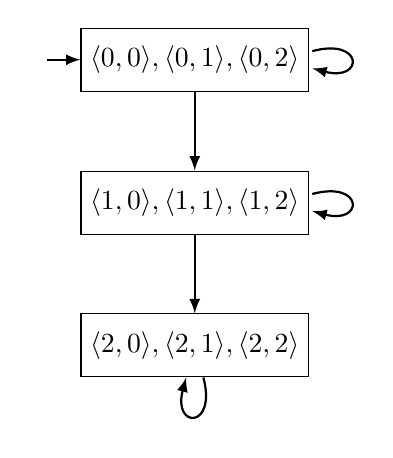
\begin{tikzpicture} [scale=2, every initial by arrow/.style={thick}]
%		\newcommand{\varstyle}[2]{\mt{\langle#1,#2\rangle}};
		
%		\node [gstate,init](x0) at (0,0) {$x=0$};
%		\node [gstate,below=of x0] (x1) {$x=1$};
%		\node [gstate,below=of x1] (x2) {$x=2$};
		\node [gstate,init](x0) at (0,0) {$\varstyle{0}{0}, \varstyle{0}{1},\varstyle{0}{2}$};
		\node [gstate,below=of x0] (x1) {$\varstyle{1}{0}, \varstyle{1}{1},\varstyle{1}{2}$};
		\node [gstate,below=of x1] (x2) {$\varstyle{2}{0}, \varstyle{2}{1},\varstyle{2}{2}$};
		
		\node [minimum size=.8cm, right=-22pt of x0] (x0loop) {};
		\node [minimum size=.8cm, right=-22pt of x1] (x1loop) {};
		
		
		
		\path [trans] (x0) edge (x1);
		\path [trans] (x1) edge (x2);
		
		\path [trans] (x0loop) edge [loop right] (x0loop);
		\path [trans] (x1loop) edge [loop right] (x1loop);
		\path [trans] (x2) edge [loop below] (x2);

		
		%		midway, at start, near start, very near start, at end, near end, very near end
		
		
	\end{tikzpicture}
\end{document}
	\end{minipage}
	\caption{Simplified representations of \mdp (left) and the \viewN \viewparamvalident on it (right)}
	\label{fig:varValIdent}  
\end{figure}


\subsection{Utilizing the MDP Graphstructure}
\subsubsection{Distance}
Considering distances in a graph can be very helpful to get an overview of a graph. Likewise it helps a lot with understanding the structure of \achgphN. In order to consider the distance between nodes we will need to formalize it.

\redcomment{definition is very simlar to execution fragments! Citation?}

\begin{definition}
	Let $\chgph = \chgphtuple$ be \achgphN. A (simple and finite) \emph{path} \path is a sequence \pathsecfull alternating between states and actions where $n \in \natnums, \{\state_1, \dots, \state_{n}\} \subseteq \states$ is a set of distinct states,  $\{\action_1, \dots, \action_{n}\} \subseteq \actions$ and for all $i \in \{1, \dots, n\}$ it is $(\state_i,\action_i, \state_{i+1}) \in \trans$. 
	
	\noindent
	It is $\pfirst(\path) := \state_1$ and $\plast(\path) := \state_n$ and \pathset the set of all paths in \chgph.
\end{definition}

\begin{definition}
	Let $\chgph = \chgphtuple$ be \achgphN. A (simple and finite) \emph{undirected path} \pathbi is a sequence \pathsecfull alternating between states and actions where $n \in \natnums, \{\state_1, \dots, \state_{n}\} \subseteq \states$ is a set of distinct states,  $\{\action_1, \dots, \action_{n}\} \subseteq \actions$ and for all $i \in \{1, \dots, n\}$ it is $(\state_i,\action_i, \state_{i+1}) \in \trans$ or $(\state_{i+1},\action_i, \state_{i}) \in \trans$. 
	
	\noindent
	It is $\pfirst(\pathbi) := \state_1$ and $\plast(\pathbi) := \state_n$ and \pathbiset the set of all undirected paths in \chgph.
\end{definition}

\begin{definition}
	\sloppy
	Let $\chgph = \chgphtuple$ be \achgphN and \path = \pathsecfull be a path in \chgph. The number $n =: \lenpath(\path)$ is called \emph{length} of the path \path.
\end{definition}

\begin{definition}
	Let $\chgph = \chgphtuple$ be \achgphN. The \emph{distance} between disjoint $\states_1, \states_2 \subseteq \states$ is the length of the shortest path from a state $\state_1 \in \states_1$ to a $\state_2 \in \states_2$. That is, if $\states_1 \cap \states_2 = \emptyset$ it is		
	\[
		\distpath(\chgph, \states_1, \states_2) := \min\{\lenpath(\path) \mid \path \in \pathset, \; \pfirst(\path) \in \states_1, \; \plast(\path) \in \states_2\},
	\]
	\noindent
	If $\states_1 \cap \states_2 \neq \emptyset$, it is $\distpath(\chgph, \states_1, \states_2) := 0$.
\end{definition}

For a given \chgphN \chgph with state set \states and $\state \in \states, \smstates \subseteq \states$ we write $\distpath(\mdp, \smstates, \state)$ short for $\distpath(\mdp, \smstates, \{\state\})$ and $\distpath(\mdp, \state, \smstates)$ short for $\distpath(\mdp, \{\state\}, \smstates)$.
For a \viewN that applies to the whole and utilizes distance it only makes sense to consider a given set of states from which one the distance is measured. An intuitive choice for such set is the set of initial states. The following algorithm calculates the distance of each node from a given set $\smstates \subseteq \states$ considering granularity \grandist:

\redcomment{Implementation Algorithm}

The set \fctdistdefault declares the returned set of \redcomment{ALGORITHM}. The implementation ensures that for every state $\state$ there exists a pair $(\state, \distval)$ in \fctdistdefault. The following view groups states that have the same distance to the set measured with the amounts of transitions necessary to reach the the closest \smstates considering the granularity \grandist.

\begin{definition}
		Let $\chgph = \chgphtuple$ be \achgphN $n \in \natnums$and $\smstates \subseteq \states$ arbitrary. \redcomment{$\fctdistdefault$ IMPLEMENTATION IN PSEUDOCODE? DEFINITION BEFORE?} The \viewN \viewdistance is defined by its \grpfctN $\gfctdistance : \states \to \imggrp$ with 
		\[
		\state \mapsto \distval - (\distval \text{ mod } n) \quad \quad \text{where } \distval = \distpath(\chgph,\smstates, \state)
		\]
		and $\imggrp = \natnums \cup \{\inf\} \cup \remset$.
\end{definition}

\begin{figure}[h]
	\begin{minipage}{.6\textwidth}
		%		\hspace{5mm}		
		\documentclass[tikz]{standalone}
%\usepackage{prelude}

%%%%%%%%%%%%%%%%%%%%%%%%%%%%%%%%%%%% PACKAGES %%%%%%%%%%%%%%%%%%%%%%%%%%%%%%%%%%%%%%%%%%

\usepackage{inputenc,fontenc}
\usepackage[a4paper,margin=3cm]{geometry}
\usepackage[english]{babel}
%\usepackage[german]{babel}
%\usepackage[fixlanguage]{babelbib}


\usepackage{bbold}
\usepackage{amsthm}
\usepackage{amsmath}
\usepackage{amssymb} % doteqdot
\usepackage[dvipsnames]{xcolor}
\usepackage{standalone}
\usepackage{tikz}[mode=buildnew]
\usepackage{cite}
\usepackage{xspace}
\usepackage{relsize}
\usepackage{mathtools} % mathclap
%\usepackage{MnSymbol}
\usepackage{hyperref}
\usepackage{url}
\usepackage{listings} % for code
\usepackage[T1]{fontenc} %<
\hypersetup{
	colorlinks,
	citecolor=black,
	filecolor=black,
	linkcolor=black,
	urlcolor=black
}
\usepackage{pgfplots}
\pgfplotsset{compat=1.18}
%\usepackage{courier} %% Sets font for listing as Courier. But also for url and texttt!
\usepackage{listings, xcolor}
\usepackage{graphicx}
\usepackage{subcaption}

\usetikzlibrary{calc}
%\usepackage{xparse} % \newDocumentCommand for multiple optional arguments
%\usepackage{titlecaps}



%%%%%%%%%%%%%%%%%%%%%%%%%%%%%%%%%%%% THEOREMSTYLES %%%%%%%%%%%%%%%%%%%%%%%%%%%%%%%%%%

\theoremstyle{definition}
\newtheorem{definition}{Definition}[section]
\newtheorem{exmp}{Beispiel}[section]
%\AfterEndEnvironment{definition}{\noindent\ignorespaces}

\theoremstyle{theorem}
\newtheorem{theorem}{Satz}[section]
\newtheorem{proposition}{Proposition}[section]
%\AfterEndEnvironment{theorem}{\noindent\ignorespaces}

\theoremstyle{korollary}
\newtheorem{korollary}{Korollar}[section]
%\AfterEndEnvironment{korollary}{\noindent\ignorespaces}


\tikzset{
	mstate/.style={draw, circle, minimum size=.94cm}, 
	gstate/.style={draw, rectangle, minimum size=.8cm},
	varstate/.style={draw,rectangle, rounded corners, minimum size=1}, 
	trans/.style={draw, ->, thick},
	bendtrans/.style={draw, ->, thick, bend left=10},
	bendtransr/.style={draw, ->, thick, bend right=10},
	init/.style={initial, initial distance=6pt, initial text=},
	every loop/.style={min distance=5pt, looseness=8},
	>=latex
}
\usetikzlibrary{automata,positioning}

%auto shift/.style={auto=right,->,
%	to path={ let \p1=(\tikztostart),\p2=(\tikztotarget),
%		\n1={atan2(\y2-\y1,\x2-\x1)},\n2={\n1+180}
%		in ($(\tikztostart.{\n1})!1mm!270:(\tikztotarget.{\n2})$) -- 
%		($(\tikztotarget.{\n2})!1mm!90:(\tikztostart.{\n1})$) \tikztonodes}},

%%%%%%%%%%%%%%%%%%%%%%%%%%%%%%%%%%% MY MACROS %%%%%%%%%%%%%%%%%%%%%%%%%%%%%%%%%%%%%%%%%
%formatting
\newcommand{\comment}[2]{{\color{#1}#2}}
\newcommand{\redcomment}[1]{{\color{red}#1}}
\newcommand{\purpcomment}[1]{{\color{pink}#1}}
\newcommand{\bluecomment}[1]{{\color{blue}#1}}
\newcommand{\mt}[1]{\ensuremath{{#1}}\xspace}
\newcommand{\mynewcommand}[2]{\newcommand{#1}{\mt{#2}}} %% currently not used becaue of ide highlighting
\newcommand{\arr}{\mt{\to}}

%model checking terms
\newcommand{\mimicrel}{\mt{\mathcal{R}}}
\newcommand{\bisimeq}{\mt{\;\!\sim\;\!}}
\newcommand{\simorder}{\mt{\;\!\preceq\;\!}}
\newcommand{\simequiv}{\mt{\;\!\simeq\;\!}} %command already defined
\newcommand{\relts}{\mt{\;\!\bullet_{_{\tiny{TS}}}\;\!}}
\newcommand{\rel}{\mt{\;\!\bullet\;\!}}

%own names
\newcommand{\nm}[1]{#1\xspace}
\newcommand{\mdpN}{\nm{MDP}}
\newcommand{\mdpsN}{\nm{MDPs}}
\newcommand{\viewN}{\nm{view}}
\newcommand{\viewNC}{\nm{View}}
\newcommand{\viewsN}{\nm{views}}
\newcommand{\viewsNC}{\nm{Views}}
\newcommand{\grpfctsubN}{\nm{detached grouping function}}
\newcommand{\grpfctsubNC}{\nm{detached grouping function}}
\newcommand{\grpfctsubNCC}{\nm{Detached Grouping Function}}
\newcommand{\grpfctN}{\nm{grouping function}}
\newcommand{\grpfctNC}{\nm{Grouping function}}
\newcommand{\grpfctNCC}{\nm{Grouping Function}}
\newcommand{\grpfctsN}{\nm{grouping functions}}
\newcommand{\grpfctsNC}{\nm{Grouping functions}}
\newcommand{\grpfctsNCC}{\nm{Grouping Functions}}
\newcommand{\stmimicN}{\nm{state-mimic}}
\newcommand{\stmimicsN}{\nm{state-mimics}}
\newcommand{\stmimickingN}{\nm{state-mimicking}}
\newcommand{\stmimickedN}{\nm{state-mimicked}}
%\newcommand{\chosenphtypeNCC}{\nm{Transition System}}
%\newcommand{\chgphNC}{\nm{Transition system}}
%\newcommand{\chgphN}{\nm{transition system}}
%\newcommand{\chgphsNCC}{\nm{Transition Systems}}
%\newcommand{\chgphsNC}{\nm{Transition systems}}
%\newcommand{\chgphsN}{\nm{transition systems}}
\newcommand{\chgphNCC}{\nm{MDP}}
\newcommand{\chgphNC}{\nm{MDP}}
\newcommand{\chgphN}{\nm{MDP}}
\newcommand{\achgphN}{\nm{an MDP}}
\newcommand{\chgphsNCC}{\nm{MDPs}}
\newcommand{\chgphsNC}{\nm{MDPs}}
\newcommand{\chgphsN}{\nm{MDPs}}
\newcommand{\parllcompN}{\nm{parallel composition}}
\newcommand{\parllcompNC}{\nm{Parallel composition}}
\newcommand{\parllcompNCC}{\nm{Parallel Composition}}
\newcommand{\parllcompsN}{\nm{parallel compositions}}
\newcommand{\parllcompsNC}{\nm{Parallel compositions}}
\newcommand{\parllcompsNCC}{\nm{Parallel Compositions}}
\newcommand{\sccN}{\nm{SCC}}
\newcommand{\sccsN}{\nm{SCCs}}
\newcommand{\bsccN}{\nm{BSCC}}
\newcommand{\bsccsN}{\nm{BSCCs}}
\newcommand{\jgrapht}{\nm{jGraphtT}}

\newcommand{\outactident}{\nm{OutActionsIdent}}

%names
\newcommand{\iffN}{\nm{if and only if}}
\newcommand{\tsN}{\nm{TS}}

%% outactions identical
\newcommand{\outactidentstrong}{\nm{strong}}
\newcommand{\outactidentweak}{\nm{weak}}

% CORE DEFINITIONS
\newcommand{\grpfct}[1][\viewppty]{\mt{F_{#1}}}
\newcommand{\grpfctsub}[1][\viewppty]{\mt{\tilde{F}_{#1}}}
%\newcommand{\grpfctimg}[1]{\mt{{\grpfct}[{#1}]}}
%\newcommand{\fctimg}[2]{\mt{{#1}[{#2}]}}
\newcommand{\eqrelview}{\mt{R}}
\newcommand{\eqclassv}[1][\state]{\mt{\eqclass{#1}{\eqrelview}}}
\newcommand{\eqclasssetv}[1][\states]{\mt{{#1}/\eqrelview}} %OLD: \bigcup_{\state \in \states} \eqclassv
\newcommand{\viewid}{\mt{\mdp}}
\newcommand{\view}[1][\viewppty]{\mt{\viewid_{#1}}}
\newcommand{\imggrp}{\mt{\arbset}}
\newcommand{\imggrpsub}{\mt{X}}
\newcommand{\viewppty}{\mt{\theta}}
\newcommand{\pll}{\mt{\;\!\pllpure\;\!}}
\newcommand{\pllrev}{\mt{\pllpure^{-1}}}
\newcommand{\pllpure}{\mt{||}}
\newcommand{\compselectset}{\mt{Z}}
\newcommand{\compselectpure}{\mt{\pllpure_\compselectset}}
\newcommand{\compselect}{\mt{\;\pllpure_\compselectset\;}}
\newcommand{\remstates}{\mt{\bigcup_{\state \in \states \setminus \states_1}\{\{\state\}\}}}
\newcommand{\nogroupstates}[1][\states_2]{\mt{\bigcup_{\state \in \states \setminus {#1}}\{\{\state\}\}}}
\newcommand{\remelem}{\mt{\bullet}}
\newcommand{\nogroupset}{\mt{\xi}}
\newcommand{\remset}{\mt{\{\remelem\}}}
\newcommand{\gfctpll}{\mt{\grpfct[\pll]}}
\newcommand{\group}{\mt{\top}}
\newcommand{\imggrpbinview}{\mt{\{\remelem, \notppty\}}}
\newcommand{\viewappset}{\mt{\tilde{\states}}}
\newcommand{\hasppty}{\mt{\top}}
\newcommand{\notppty}{\mt{\bot}}
\newcommand{\disregardelem}{\mt{\Delta}}
\newcommand{\disregardelements}{\mt{{\disregardelem_1, \dots, \disregardelem_n}}}



%\newcommand{\mdp}{def}\mdp
%\newcommand{\mdpdef}



% EXAMPLE VIEWS
\newcommand{\pptyatomicprops}{\mt{\atomicprops}}
\newcommand{\pptyinitstates}{\mt{\initstates}}
\newcommand{\pptyinactsetsize}{\mt{|\inacts(\state)|}}
\newcommand{\pptyhasoutact}{\mt{\exists\outact}}
\newcommand{\pptyminoutact}[2]{\mt{#1\leq#2}}
\newcommand{\pptymaxoutact}[2]{\mt{#2\leq#1}}
\newcommand{\pptyspanoutact}[3]{\mt{#1\leq#2\leq#3}}
\newcommand{\pptyoutactsetsize}{\mt{|\outacts(\state)|}}
\newcommand{\pptyoutactsingle}{\mt{|\outacts(\state)|_1}}
\newcommand{\pptystrongoutactident}{\mt{\outacts(\state)_=}}
\newcommand{\pptyweakoutactident}{\mt{\outacts(\state)_\approx}}
\newcommand{\pptyhasinact}{\mt{\exists\inact}}
\newcommand{\pptymininact}[2]{\mt{#1\leq#2}}
\newcommand{\pptymaxinact}[2]{\mt{#2\leq#1}}
\newcommand{\pptyspaninact}[3]{\mt{#1\leq#2\leq#3}}
\newcommand{\pptyinactsingle}{\mt{|\inacts(\state)|_1}}
\newcommand{\pptystronginactident}{\mt{\inacts(\state)_=}}
\newcommand{\pptyweakinactident}{\mt{\inacts(\state)_\approx}}
\newcommand{\pptyparamvalueseq}{\mt{\var = \varval}}
\newcommand{\pptyparamvaluesneq}{\mt{\var \neq \varval}}
\newcommand{\pptyparamdnf}{\mt{VarDNF}}
\newcommand{\pptyparamcnf}{\mt{VarCNF}}
\newcommand{\pptyparamvalueseqopt}{\mt{\var = \varval}}
\newcommand{\pptyparamvalident}{\mt{Var:\varval}}
\newcommand{\pptydistance}{\mt{\distpath}}
\newcommand{\pptydistancerev}{\mt{\distpathrev}}
\newcommand{\pptydistancebi}{\mt{\distpathbi}}
\newcommand{\pptyhascycle}{\mt{\exists\cycle}}
\newcommand{\pptyexactactcycle}{\mt{\{\cycle_{\action,n}\}}}
\newcommand{\pptycycleset}{\mt{\cup{\{\state\}_\cycle}}}
\newcommand{\pptyexactcycle}{\mt{\{\cycle_n\}}}
\newcommand{\pptyscc}{\mt{scc}}
\newcommand{\pptybscc}{\mt{bscc}}
\newcommand{\pptyprop}{\mt{\redcomment{?}}}
\newcommand{\pptyident}{id}


\newcommand{\gfctatomicprops}{\mt{\grpfct[\pptyatomicprops]}}
\newcommand{\gfctinitstates}{\mt{\grpfct[\pptyinitstates]^\hasppty}}
\newcommand{\gfcthasoutaction}{\mt{\grpfct[\pptyhasoutact]^\hasppty}}
\newcommand{\gfctminoutaction}{\mt{\grpfct[\pptyminoutact{\numoutact}{\outact}]^\hasppty}}
\newcommand{\gfctmaxoutaction}{\mt{\grpfct[\pptymaxoutact{\numoutact}{\outact}]^\hasppty}}
\newcommand{\gfctspanoutaction}{\mt{\grpfct[\pptyspanoutact{\numoutactb}{\outact}{\numoutact}]^\hasppty}}
\newcommand{\gfctoutactsetsize}{\mt{\grpfct[\pptyoutactsetsize]}}
\newcommand{\gfctoutactsingle}{\mt{\grpfct[\pptyoutactsingle]^\notppty}}
\newcommand{\gfctstrongoutactident}{\mt{\grpfct[\pptystrongoutactident]}}
\newcommand{\gfctweakoutactident}{\mt{\grpfct[\pptyweakoutactident]}}
\newcommand{\gfcthasinaction}{\mt{\grpfct[\pptyhasinact]^\hasppty}}
\newcommand{\gfctmininaction}{\mt{\grpfct[\pptymininact{\numinact}{\inact}]^\hasppty}}
\newcommand{\gfctmaxinaction}{\mt{\grpfct[\pptymaxinact{\numinact}{\inact}]^\hasppty}}
\newcommand{\gfctspaninaction}{\mt{\grpfct[\pptyspaninact{\numinactb}{\inact}{\numinact}]^\hasppty}}
\newcommand{\gfctinactsetsize}{\mt{\grpfct[\pptyinactsetsize]}}
\newcommand{\gfctinactsingle}{\mt{\grpfct[\pptyinactsingle]^\notppty}}
\newcommand{\gfctstronginactident}{\mt{\grpfct[\pptystronginactident]}}
\newcommand{\gfctweakinactident}{\mt{\grpfct[\pptyweakinactident]}}
\newcommand{\gfctparamvalueseq}{\mt{\grpfct[\pptyparamvalueseq]^\hasppty}}
\newcommand{\gfctparamvaluesneq}{\mt{\grpfct[\pptyparamvaluesneq]^\hasppty}}
\newcommand{\gfctparamdnf}{\mt{\grpfct[\pptyparamdnf]^\hasppty}}
\newcommand{\gfctparamcnf}{\mt{\grpfct[\pptyparamcnf]^\hasppty}}
\newcommand{\gfctparamvalueseqopt}{\mt{\pptyparamvalueseqopt}}
\newcommand{\gfctparamvalident}{\mt{\grpfct[\pptyparamvalident]}}
\newcommand{\gfctdistance}{\mt{\grpfct[\pptydistance]}}
\newcommand{\gfctdistancerev}{\mt{\grpfct[\pptydistancerev]}}
\newcommand{\gfctdistancebi}{\mt{\grpfct[\pptydistancebi]}}
\newcommand{\gfcthascycle}{\mt{\grpfct[\pptyhascycle]}}
\newcommand{\gfctexactcycle}{\mt{\grpfct[\pptyexactcycle]}}
\newcommand{\gfctcycleset}{\mt{\grpfct[\pptycycleset]}}
\newcommand{\gfctexactactcycle}{\mt{\grpfct[\pptyexactactcycle]}}
\newcommand{\gfctscc}{\mt{\grpfct[\pptyscc]}}
\newcommand{\gfctbscc}{\mt{\grpfct[\pptybscc]}}
\newcommand{\gfctprop}{\mt{\grpfct[\pptyprop]}}
\newcommand{\gfctident}{\mt{\grpfct[\pptyident]}}

\newcommand{\gfctsubatomicprops}{\mt{\grpfctsub[\pptyatomicprops]}}
\newcommand{\gfctsubinitstates}{\mt{\grpfctsub[\pptyinitstates]^\hasppty}}
\newcommand{\gfctsubhasoutaction}{\mt{\grpfctsub[\pptyhasoutact]^\hasppty}}
\newcommand{\gfctsubminoutaction}{\mt{\grpfctsub[\pptyminoutact{\numoutact}{\outact}]^\hasppty}}
\newcommand{\gfctsubmaxoutaction}{\mt{\grpfctsub[\pptymaxoutact{\numoutact}{\outact}]^\hasppty}}
\newcommand{\gfctsubspanoutaction}{\mt{\grpfctsub[\pptyspanoutact{\numoutactb}{\outact}{\numoutact}]^\hasppty}}
\newcommand{\gfctsuboutactsetsize}{\mt{\grpfctsub[\pptyoutactsetsize]}}
\newcommand{\gfctsuboutactsingle}{\mt{\grpfctsub[\pptyoutactsingle]^\notppty}}
\newcommand{\gfctsubstrongoutactident}{\mt{\grpfctsub[\pptystrongoutactident]^\hasppty}}
\newcommand{\gfctsubweakoutactident}{\mt{\grpfctsub[\pptyweakoutactident]^\hasppty}}
\newcommand{\gfctsubhasinaction}{\mt{\grpfctsub[\pptyhasinact]}}
\newcommand{\gfctsubmininaction}{\mt{\grpfctsub[\pptymininact{\numinact}{\inact}]}}
\newcommand{\gfctsubmaxinaction}{\mt{\grpfctsub[\pptymaxinact{\numinact}{\inact}]}}
\newcommand{\gfctsubspaninaction}{\mt{\grpfctsub[\pptyspaninact{\numinactb}{\inact}{\numinact}]}}
\newcommand{\gfctsubinactsetsize}{\mt{\grpfctsub[\pptyinactsetsize]^\hasppty}}
\newcommand{\gfctsubinactsingle}{\mt{\grpfctsub[\pptyinactsingle]^\notppty}}
\newcommand{\gfctsubstronginactident}{\mt{\grpfctsub[\pptystronginactident]}}
\newcommand{\gfctsubweakinactident}{\mt{\grpfctsub[\pptyweakinactident]}}
\newcommand{\gfctsubparamvalueseq}{\mt{\grpfctsub[\pptyparamvalueseq]^\hasppty}}
\newcommand{\gfctsubparamvaluesneq}{\mt{\grpfctsub[\pptyparamvaluesneq]^\hasppty}}
\newcommand{\gfctsubparamdnf}{\mt{\grpfctsub[\pptyparamdnf]^\hasppty}}
\newcommand{\gfctsubparamcnf}{\mt{\grpfctsub[\pptyparamcnf]^\hasppty}}
\newcommand{\gfctsubparamvalueseqopt}{\mt{\pptyparamvalueseqopt}}
\newcommand{\gfctsubparamvalident}{\mt{\grpfctsub[\pptyparamvalident]}}
\newcommand{\gfctsubdistance}{\mt{\grpfctsub[\pptydistance]}}
\newcommand{\gfctsubdistancerev}{\mt{\grpfctsub[\pptydistancerev]}}
\newcommand{\gfctsubdistancebi}{\mt{\grpfctsub[\pptydistancebi]}}
\newcommand{\gfctsubhascycle}{\mt{\grpfctsub[\pptyhascycle]^\hasppty}}
\newcommand{\gfctsubexactcycle}{\mt{\grpfctsub[\pptyexactcycle]}}
\newcommand{\gfctsubcycleset}{\mt{\grpfctsub[\pptycycleset]}}
\newcommand{\gfctsubexactactcycle}{\mt{\grpfctsub[\pptyexactactcycle]}}
\newcommand{\gfctsubscc}{\mt{\grpfctsub[\pptyscc]}}
\newcommand{\gfctsubbscc}{\mt{\grpfctsub[\pptybscc]}}
\newcommand{\gfctsubprop}{\mt{\grpfctsub[\pptyprop]}}
\newcommand{\gfctsubident}{\mt{\grpfctsub[\pptyident]}}


\newcommand{\viewatomicprops}{\mt{\view[\pptyatomicprops]}}
\newcommand{\viewinitstates}{\mt{\view[\pptyinitstates]^\hasppty}}
\newcommand{\viewhasoutaction}{\mt{\view[\pptyhasoutact]^\hasppty}}
\newcommand{\viewminoutaction}{\mt{\view[\pptyminoutact{\numoutact}{\outact}]^\hasppty}}
\newcommand{\viewmaxoutaction}{\mt{\view[\pptymaxoutact{\numoutact}{\outact}]^\hasppty}}
\newcommand{\viewspanoutaction}{\mt{\view[\pptyspanoutact{\numoutactb}{\outact}{\numoutact}]^\hasppty}}
\newcommand{\viewoutactsetsize}{\mt{\view[\pptyoutactsetsize]}}
\newcommand{\viewoutactsingle}{\mt{\view[\pptyoutactsingle]^\notppty}}
\newcommand{\viewstrongoutactident}{\mt{\view[\pptystrongoutactident]}}
\newcommand{\viewweakoutactident}{\mt{\view[\pptyweakoutactident]}}
\newcommand{\viewhasinaction}{\mt{\view[\pptyhasinact]^\hasppty}}
\newcommand{\viewmininaction}{\mt{\view[\pptymininact{\numinact}{\inact}]^\hasppty}}
\newcommand{\viewmaxinaction}{\mt{\view[\pptymaxinact{\numinact}{\inact}]^\hasppty}}
\newcommand{\viewspaninaction}{\mt{\view[\pptyspaninact{\numinactb}{\inact}{\numinact}]^\hasppty}}
\newcommand{\viewinactsetsize}{\mt{\view[\pptyinactsetsize]}}
\newcommand{\viewinactsingle}{\mt{\view[\pptyinactsingle]^\notppty}}
\newcommand{\viewstronginactident}{\mt{\view[\pptystronginactident]}}
\newcommand{\viewweakinactident}{\mt{\view[\pptyweakinactident]}}
\newcommand{\viewparamvalueseq}{\mt{\view[\pptyparamvalueseq]}}
\newcommand{\viewparamvaluesneq}{\mt{\view[\pptyparamvaluesneq]}}
\newcommand{\viewparamdnf}{\mt{\view[\pptyparamdnf]^\hasppty}}
\newcommand{\viewparamcnf}{\mt{\view[\pptyparamcnf]^\hasppty}}
\newcommand{\viewparamvalueseqopt}{\mt{\pptyparamvalueseqopt}}
\newcommand{\viewparamvalident}{\mt{\view[\pptyparamvalident]}}
\newcommand{\viewdistance}{\mt{\view[\pptydistance]}}
\newcommand{\viewdistancerev}{\mt{\view[\pptydistancerev]}}
\newcommand{\viewdistancebi}{\mt{\view[\pptydistancebi]}}
\newcommand{\viewhascycle}{\mt{\view[\pptyhascycle]}}
\newcommand{\viewexactcycle}{\mt{\view[\pptyexactcycle]}}
\newcommand{\viewcycleset}{\mt{\view[\pptycycleset]}}
\newcommand{\viewexactactcycle}{\mt{\view[\pptyexactactcycle]}}
\newcommand{\viewscc}{\mt{\view[\pptyscc]}}
\newcommand{\viewbscc}{\mt{\view[\pptybscc]}}
\newcommand{\viewprop}{\mt{\view[\pptyprop]}}
\newcommand{\viewident}{\mt{\view[\pptyident]}}

%\newcommand{\viewatomicprops}{\mt{\view[\atomicprops]}}
%\newcommand{\viewinitstates}{\mt{\view[\initstates]}}
%\newcommand{\viewhasoutaction}{\mt{\view[\pptyhasoutact]}}
%\newcommand{\viewminoutaction}{\mt{\view[\pptyminoutact{\numoutact}{\outact}]}}
%\newcommand{\viewmaxoutaction}{\mt{\view[\pptymaxoutact{\numoutact}{\outact}]}}
%\newcommand{\viewspanoutaction}{\mt{\view[\pptyspanoutact{\numoutactb}{\outact}{\numoutact}]}}
%\newcommand{\viewoutactsetsize}{\mt{\view[\pptyoutactsetsize]}}
%\newcommand{\viewoutactsingle}{\mt{\view[\pptyoutactsingle]}}
%\newcommand{\viewstrongoutactident}{\mt{\view[\outacts(\state)_=]}}
%\newcommand{\viewweakoutactident}{\mt{\view[\outacts(\state)_\approx]}}
%\newcommand{\viewhasinaction}{\mt{\view[\pptyhasinact]}}
%\newcommand{\viewmininaction}{\mt{\view[\pptymininact{\numinact}{\inact}]}}
%\newcommand{\viewmaxinaction}{\mt{\view[\pptymaxinact{\numinact}{\inact}]}}
%\newcommand{\viewspaninaction}{\mt{\view[\pptyspaninact{\numinactb}{\inact}{\numinact}]}}
%\newcommand{\viewinactsetsize}{\mt{\view[\pptyinactsetsize]}}
%\newcommand{\viewinactsingle}{\mt{\view[\pptyinactsingle]}}
%\newcommand{\viewstronginactident}{\mt{\view[\inacts(\state)_=]}}
%\newcommand{\viewweakinactident}{\mt{\view[\inacts(\state)_\approx]}}
%\newcommand{\viewparamvalueseq}{\mt{\view[\var = \varval]}}
%\newcommand{\viewparamvaluesneq}{\mt{\view[\var \neq \varval]}}
%\newcommand{\viewparamdnf}{\mt{\view[VarDNF]}}
%\newcommand{\viewparamcnf}{\mt{\view[VarCNF]}}
%\newcommand{\viewparamvalident}{\mt{\view[\pptyparamvalident]}}
%\newcommand{\viewdistance}{\mt{\view[\pptydistance]}}
%\newcommand{\viewhascycle}{\mt{\view[\exists\cycle]}}
%\newcommand{\viewexactcycle}{\mt{\view[\pptyexactcycle]}}
%\newcommand{\viewcycleset}{\mt{\view[\pptycycleset]}}
%\newcommand{\viewexactactcycle}{\mt{\view[\pptyexactactcycle]}}
%\newcommand{\viewscc}{\mt{\view[scc]}}
%\newcommand{\viewbscc}{\mt{\view[bscc]}}

%actions
\newcommand{\numoutact}{\mt{n}}
\newcommand{\numoutactb}{\mt{m}}
\newcommand{\numinact}{\mt{n}}
\newcommand{\numinactb}{\mt{m}}

\newcommand{\predmaxoutact}[1][\numoutact]{\mt{Q_{\outact\leq#1}(\state,\state_1, \dots, \state_{#1+1})}}
\newcommand{\predminoutact}[1][\numoutact]{\mt{Q_{#1\leq\outact}(\state,\state_1, \dots, \state_{#1})}}
\newcommand{\formoutact}[1][\state]{\mt{C_{#1,\outact}}}
\newcommand{\predmaxinact}[1][\numinact]{\mt{Q_{\inact\leq#1}(\state,\state_1, \dots, \state_{#1+1})}}
\newcommand{\predmininact}[1][\numinact]{\mt{Q_{#1\leq\inact}(\state,\state_1, \dots, \state_{#1})}}

\newcommand{\outact}[1][\action]{\mt{\overrightarrow{#1}}}
\newcommand{\outacts}{\mt{\overrightarrow{\actions}}}
\newcommand{\inact}{\mt{\overleftarrow{\action}}}
\newcommand{\inacts}[1][\action]{\mt{\overleftarrow{#1}}}

%%Parameters
\newcommand{\vars}[1][\mdp]{\mt{V\!ar_{#1}}}
\newcommand{\var}{\mt{x}}
\newcommand{\varstate}[1][]{\mt{\var_{\state#1}}}
\newcommand{\varval}{\mt{a}}
\newcommand{\vareval}[1][\mdp]{\mt{V\!arEval_{#1}}}
\newcommand{\varevalimg}[1][\mdp]{\mt{\vareval[#1][\states,\vars]}}
\newcommand{\varevalimgset}{\mt{\arbset}}
\newcommand{\someparam}{\mt{\tilde{x}}}
\newcommand{\eqorneq}{\mt{\;\doteqdot\;}}
\newcommand{\varstyle}[2]{\mt{\langle#1,#2\rangle}}




%\makeatletter
%\newcommand{\overleftrightsmallarrow}{\mathpalette{\overarrowsmall@\leftrightarrowfill@}}
%\newcommand{\overrightsmallarrow}{\mathpalette{\overarrowsmall@\rightarrowfill@}}
%\newcommand{\overleftsmallarrow}{\mathpalette{\overarrowsmall@\leftarrowfill@}}
%\newcommand{\overarrowsmall@}[3]{%
%	\vbox{%
%		\ialign{%
%			##\crcr
%			#1{\smaller@style{#2}}\crcr
%			\noalign{\nointerlineskip}%
%			$\m@th\hfil#2#3\hfil$\crcr
%		}%
%	}%
%}
%\def\smaller@style#1{%
%	\ifx#1\displaystyle\scriptstyle\else
%	\ifx#1\textstyle\scriptstyle\else
%	\scriptscriptstyle
%	\fi
%	\fi
%}
%\makeatother
%\newcommand{\te}[1]{\overleftrightsmallarrow{#1}}

% Distance
\newcommand{\fctdist}{\mt{distance}}
\newcommand{\fctdistdefault}{\mt{\fctdist(\chgph, \smstates, \grandist)}}
\newcommand{\distval}{\mt{d}}
\newcommand{\grandist}{\mt{n}}
\let\path\oldpath
\newcommand{\path}{\mt{P}}
\newcommand{\pathbi}{\mt{\bar{\path}}}
\newcommand{\pathsecfull}{\mt{(\state_0, \action_0, \state_1, \action_1, \dots, \action_{n}, \state_{n+1})}}
\newcommand{\lenpath}{\mt{len}}
\newcommand{\pfirst}{\mt{first}}
\newcommand{\plast}{\mt{last}}
\newcommand{\pathset}{\mt{\path_\chgph}}
\newcommand{\pathbiset}{\mt{\pathbi_\chgph}}
\newcommand{\distpath}{\mt{\overrightarrow{dist}}}
\newcommand{\distpathrev}{\mt{\overleftarrow{dist}}}
\newcommand{\distpathbi}{\mt{\overline{dist}}}
%Cycles
\newcommand{\cyclesecfull}{\mt{(\state_0, \action_0, \state_1, \action_1, \dots, \action_{n-1}, \state_0)}}
\newcommand{\fctfindcycles}{\mt{findCycles}}
\newcommand{\cycle}{\mt{C}}
\newcommand{\cycleset}{\mt{\cycle_{\mdp, n}}}
\newcommand{\lencycle}{\mt{len}}
% strongly connected components
\newcommand{\scc}{\mt{T}}
\newcommand{\setscc}{\mt{SCC_{\chgph,n}}}
\newcommand{\setbscc}{\mt{BSCC_{\chgph,n}}}

% properties
\newcommand{\propfct}{\mt{f}}

% all Systems
\newcommand{\chgph}{\mt{\mdp}}
\newcommand{\chgphtuple}{\mt{\mdptuple}}
\newcommand{\chgphtupledist}{\mt{\mdptupledist}}

\newcommand{\states}{\mt{S}}
\newcommand{\actions}{\mt{Act}}
\newcommand{\atomicprops}{\mt{AP}}
\newcommand{\labelingfct}{\mt{L}}
\newcommand{\init}{\mt{\initdistrib}} % use MDP % refers to the underlying set
\newcommand{\trans}{\mt{\probtfunc}} % use MDP % refers to the underlying set
\newcommand{\smstates}{\mt{\tilde{\states}}}


\newcommand{\state}{\mt{s}}
\newcommand{\action}{\mt{\alpha}}
\newcommand{\actionb}{\mt{\beta}}
\newcommand{\actionc}{\mt{\gamma}}
\newcommand{\smstate}{\mt{\tilde{\state}}}



% transition sysstems
\newcommand{\ts}{\mt{TS}}
\newcommand{\transitionrel}{\mt{\longrightarrow}}
\newcommand{\initstates}{\mt{I}}
\newcommand{\transitionsystem}{\mt
	{(\states, \actions, \transitionrel, \initstates, \atomicprops, \labelingfct)}
}
\newcommand{\tstupledist}{\mt{(\states', \actions',\transitionrel', \initstates', \labelingfct')}}


%Markov chains and MDP
\newcommand{\mdp}{\mt{\autm}}
\newcommand{\mdptuple}{\mt{(\states, \actions, \probtfunc, \initdistrib, \atomicprops, \labelingfct)}}
\newcommand{\mdptupledist}{\mt{(\states', \actions', \probtfunc', \initdistrib', \atomicprops', \labelingfct')}}
\newcommand{\autm}{\mt{\mathcal{M}}}
\newcommand{\probtfunc}{\mt{\textbf{P}}}
\newcommand{\initdistrib}{\mt{\iota_{init}}}


%maths
\newcommand{\powerset}[1]{\mt{\mathcal{P}(#1)}}
\newcommand{\eqclass}[2]{\mt{[#1]_{#2}}}%{\mt{#1 / #2}}
\newcommand{\impr}{\mt{\hspace{3mm}\Rightarrow\hspace{2mm}}}
\newcommand{\impl}{\mt{\hspace{3mm}\Leftarrow\hspace{2mm}}}
\newcommand{\natnums}{\mt{\mathbb{N}}} 
\newcommand{\realnums}{\mt{\mathbb{R}}}
\newcommand{\intmodn}[1][n]{\mt{\mathbb{Z}_{#1}}}
\newcommand{\arbset}{\mt{M}}
\newcommand{\bigsum}[2][]{\mt{\mathlarger{\sum}_{#2}^{#1}}}
\newcommand{\bbigsum}[2][]{\mt{\mathlarger{\mathlarger{\sum}}_{#2}^{#1}}}
\newcommand{\invimage}[2]{#1^{\mt{-1}(#2)}}
\newcommand{\img}{\mt{Img}}
\newcommand{\cond}{\mt{\,|\,}}

%tickz
%% \definecolor{darkred}{RGB}{196, 42, 42}

%implementation
\newcommand{\pmcvis}{\nm{PMC-Vis}}


\usepackage{tikz}
\newcommand{\stateppty}{draw, circle, minimum size=1cm}


\begin{document}
	\newcommand{\createstate}[3]{\node[draw, circle, minimum size=1cm] (#1) at (#2) {#3}}
	\newcommand{\basex}{0}
	\newcommand{\basey}{0}
	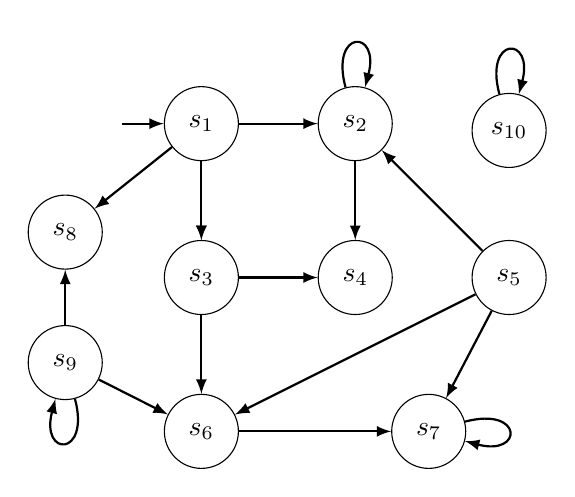
\begin{tikzpicture} [every initial by arrow/.style={thick}]
		%		\createstate{s1}{3,2+4}{$\state_1$};
		\path 
		(\basex,  \basey+2) node[mstate, initial, initial text=, initial distance=15pt] (s1) {$\state_1$} 
		;
		
		\node [mstate,right=of s1] (s2) {$\state_2$};
		\node [mstate,below=of s1] (s3) {$\state_3$};
		\node [mstate,below=of s2] (s4) {$\state_4$};
		\node [mstate,right=of s4] (s5) {$\state_5$};
		%		\node [mstate,below right=40pt and 30 pt of s2] (s5) {$\state_5$};
		\node [mstate,below=of s3] (s6) {$\state_6$};
		\node [mstate,right=55pt of s6] (s7) {$\state_7$};
		\node [mstate,below left=20pt and 30pt of s1] (s8) {$\state_8$};
		\node [mstate,below=20pt of s8] (s9) {$\state_9$};
		%		\node [mstate,right=of s2] (s10) {$\state_{10}$};
		\node [mstate,above=26pt of s5] (s10) {$\state_{10}$};
		
%		\node [above right=-4pt of s1] (ls1) {$\{\}$};
%		\node [above right=-6pt of s2] (ls2) {$\{a,b\}$};
%		\node [above right=-4pt of s3] (ls3) {$\{a,b\}$};
%		\node [above right=0pt and -8pt of s4] (ls4) {$\{a\}$};
%		\node [above right=-4pt of s5] (ls5) {$\{b\}$};
%		\node [below left=-4pt of s6] (ls6) {$\{a,b\}$};
%		\node [below left=-4pt of s7] (ls7) {$\{b\}$};
%		\node [above left=-4pt of s8] (ls8) {$\{a\}$};
%		\node [above left=-4pt of s9] (ls9) {$\{a\}$};
%		\node [above right=-4pt of s10] (ls10) {$\{\}$};
		
		
		
		
		\path [trans] (s1) edge (s2);
		\path [trans] (s1) edge (s3);
		\path [trans] (s1) edge (s3);
		\path [trans] (s1) edge (s8);
		\path [trans] (s2) edge (s4);
		\path [trans] (s3) edge (s4);
		\path [trans] (s3) edge (s6);
		\path [trans] (s5) edge (s2);
		\path [trans] (s5) edge (s6);
		\path [trans] (s5) edge (s7);
		\path [trans] (s6) edge (s7);
		\path [trans] (s9) edge (s8);
		\path [trans] (s9) edge (s6);
		
		\path [trans] (s2) edge [loop above] (s2);
		\path [trans] (s7) edge [loop right] (s7);
		\path [trans] (s9) edge [loop below] (s9);
		\path [trans] (s10) edge [loop above] (s10);
		
	\end{tikzpicture}
\end{document}
	\end{minipage}%
	\begin{minipage}{.5\textwidth}
		\documentclass[tikz,preview]{standalone}
%\usepackage{prelude}

%%%%%%%%%%%%%%%%%%%%%%%%%%%%%%%%%%%% PACKAGES %%%%%%%%%%%%%%%%%%%%%%%%%%%%%%%%%%%%%%%%%%

\usepackage{inputenc,fontenc}
\usepackage[a4paper,margin=3cm]{geometry}
\usepackage[english]{babel}
%\usepackage[german]{babel}
%\usepackage[fixlanguage]{babelbib}


\usepackage{bbold}
\usepackage{amsthm}
\usepackage{amsmath}
\usepackage{amssymb} % doteqdot
\usepackage[dvipsnames]{xcolor}
\usepackage{standalone}
\usepackage{tikz}[mode=buildnew]
\usepackage{cite}
\usepackage{xspace}
\usepackage{relsize}
\usepackage{mathtools} % mathclap
%\usepackage{MnSymbol}
\usepackage{hyperref}
\usepackage{url}
\usepackage{listings} % for code
\usepackage[T1]{fontenc} %<
\hypersetup{
	colorlinks,
	citecolor=black,
	filecolor=black,
	linkcolor=black,
	urlcolor=black
}
\usepackage{pgfplots}
\pgfplotsset{compat=1.18}
%\usepackage{courier} %% Sets font for listing as Courier. But also for url and texttt!
\usepackage{listings, xcolor}
\usepackage{graphicx}
\usepackage{subcaption}

\usetikzlibrary{calc}
%\usepackage{xparse} % \newDocumentCommand for multiple optional arguments
%\usepackage{titlecaps}



%%%%%%%%%%%%%%%%%%%%%%%%%%%%%%%%%%%% THEOREMSTYLES %%%%%%%%%%%%%%%%%%%%%%%%%%%%%%%%%%

\theoremstyle{definition}
\newtheorem{definition}{Definition}[section]
\newtheorem{exmp}{Beispiel}[section]
%\AfterEndEnvironment{definition}{\noindent\ignorespaces}

\theoremstyle{theorem}
\newtheorem{theorem}{Satz}[section]
\newtheorem{proposition}{Proposition}[section]
%\AfterEndEnvironment{theorem}{\noindent\ignorespaces}

\theoremstyle{korollary}
\newtheorem{korollary}{Korollar}[section]
%\AfterEndEnvironment{korollary}{\noindent\ignorespaces}


\tikzset{
	mstate/.style={draw, circle, minimum size=.94cm}, 
	gstate/.style={draw, rectangle, minimum size=.8cm},
	varstate/.style={draw,rectangle, rounded corners, minimum size=1}, 
	trans/.style={draw, ->, thick},
	bendtrans/.style={draw, ->, thick, bend left=10},
	bendtransr/.style={draw, ->, thick, bend right=10},
	init/.style={initial, initial distance=6pt, initial text=},
	every loop/.style={min distance=5pt, looseness=8},
	>=latex
}
\usetikzlibrary{automata,positioning}

%auto shift/.style={auto=right,->,
%	to path={ let \p1=(\tikztostart),\p2=(\tikztotarget),
%		\n1={atan2(\y2-\y1,\x2-\x1)},\n2={\n1+180}
%		in ($(\tikztostart.{\n1})!1mm!270:(\tikztotarget.{\n2})$) -- 
%		($(\tikztotarget.{\n2})!1mm!90:(\tikztostart.{\n1})$) \tikztonodes}},

%%%%%%%%%%%%%%%%%%%%%%%%%%%%%%%%%%% MY MACROS %%%%%%%%%%%%%%%%%%%%%%%%%%%%%%%%%%%%%%%%%
%formatting
\newcommand{\comment}[2]{{\color{#1}#2}}
\newcommand{\redcomment}[1]{{\color{red}#1}}
\newcommand{\purpcomment}[1]{{\color{pink}#1}}
\newcommand{\bluecomment}[1]{{\color{blue}#1}}
\newcommand{\mt}[1]{\ensuremath{{#1}}\xspace}
\newcommand{\mynewcommand}[2]{\newcommand{#1}{\mt{#2}}} %% currently not used becaue of ide highlighting
\newcommand{\arr}{\mt{\to}}

%model checking terms
\newcommand{\mimicrel}{\mt{\mathcal{R}}}
\newcommand{\bisimeq}{\mt{\;\!\sim\;\!}}
\newcommand{\simorder}{\mt{\;\!\preceq\;\!}}
\newcommand{\simequiv}{\mt{\;\!\simeq\;\!}} %command already defined
\newcommand{\relts}{\mt{\;\!\bullet_{_{\tiny{TS}}}\;\!}}
\newcommand{\rel}{\mt{\;\!\bullet\;\!}}

%own names
\newcommand{\nm}[1]{#1\xspace}
\newcommand{\mdpN}{\nm{MDP}}
\newcommand{\mdpsN}{\nm{MDPs}}
\newcommand{\viewN}{\nm{view}}
\newcommand{\viewNC}{\nm{View}}
\newcommand{\viewsN}{\nm{views}}
\newcommand{\viewsNC}{\nm{Views}}
\newcommand{\grpfctsubN}{\nm{detached grouping function}}
\newcommand{\grpfctsubNC}{\nm{detached grouping function}}
\newcommand{\grpfctsubNCC}{\nm{Detached Grouping Function}}
\newcommand{\grpfctN}{\nm{grouping function}}
\newcommand{\grpfctNC}{\nm{Grouping function}}
\newcommand{\grpfctNCC}{\nm{Grouping Function}}
\newcommand{\grpfctsN}{\nm{grouping functions}}
\newcommand{\grpfctsNC}{\nm{Grouping functions}}
\newcommand{\grpfctsNCC}{\nm{Grouping Functions}}
\newcommand{\stmimicN}{\nm{state-mimic}}
\newcommand{\stmimicsN}{\nm{state-mimics}}
\newcommand{\stmimickingN}{\nm{state-mimicking}}
\newcommand{\stmimickedN}{\nm{state-mimicked}}
%\newcommand{\chosenphtypeNCC}{\nm{Transition System}}
%\newcommand{\chgphNC}{\nm{Transition system}}
%\newcommand{\chgphN}{\nm{transition system}}
%\newcommand{\chgphsNCC}{\nm{Transition Systems}}
%\newcommand{\chgphsNC}{\nm{Transition systems}}
%\newcommand{\chgphsN}{\nm{transition systems}}
\newcommand{\chgphNCC}{\nm{MDP}}
\newcommand{\chgphNC}{\nm{MDP}}
\newcommand{\chgphN}{\nm{MDP}}
\newcommand{\achgphN}{\nm{an MDP}}
\newcommand{\chgphsNCC}{\nm{MDPs}}
\newcommand{\chgphsNC}{\nm{MDPs}}
\newcommand{\chgphsN}{\nm{MDPs}}
\newcommand{\parllcompN}{\nm{parallel composition}}
\newcommand{\parllcompNC}{\nm{Parallel composition}}
\newcommand{\parllcompNCC}{\nm{Parallel Composition}}
\newcommand{\parllcompsN}{\nm{parallel compositions}}
\newcommand{\parllcompsNC}{\nm{Parallel compositions}}
\newcommand{\parllcompsNCC}{\nm{Parallel Compositions}}
\newcommand{\sccN}{\nm{SCC}}
\newcommand{\sccsN}{\nm{SCCs}}
\newcommand{\bsccN}{\nm{BSCC}}
\newcommand{\bsccsN}{\nm{BSCCs}}
\newcommand{\jgrapht}{\nm{jGraphtT}}

\newcommand{\outactident}{\nm{OutActionsIdent}}

%names
\newcommand{\iffN}{\nm{if and only if}}
\newcommand{\tsN}{\nm{TS}}

%% outactions identical
\newcommand{\outactidentstrong}{\nm{strong}}
\newcommand{\outactidentweak}{\nm{weak}}

% CORE DEFINITIONS
\newcommand{\grpfct}[1][\viewppty]{\mt{F_{#1}}}
\newcommand{\grpfctsub}[1][\viewppty]{\mt{\tilde{F}_{#1}}}
%\newcommand{\grpfctimg}[1]{\mt{{\grpfct}[{#1}]}}
%\newcommand{\fctimg}[2]{\mt{{#1}[{#2}]}}
\newcommand{\eqrelview}{\mt{R}}
\newcommand{\eqclassv}[1][\state]{\mt{\eqclass{#1}{\eqrelview}}}
\newcommand{\eqclasssetv}[1][\states]{\mt{{#1}/\eqrelview}} %OLD: \bigcup_{\state \in \states} \eqclassv
\newcommand{\viewid}{\mt{\mdp}}
\newcommand{\view}[1][\viewppty]{\mt{\viewid_{#1}}}
\newcommand{\imggrp}{\mt{\arbset}}
\newcommand{\imggrpsub}{\mt{X}}
\newcommand{\viewppty}{\mt{\theta}}
\newcommand{\pll}{\mt{\;\!\pllpure\;\!}}
\newcommand{\pllrev}{\mt{\pllpure^{-1}}}
\newcommand{\pllpure}{\mt{||}}
\newcommand{\compselectset}{\mt{Z}}
\newcommand{\compselectpure}{\mt{\pllpure_\compselectset}}
\newcommand{\compselect}{\mt{\;\pllpure_\compselectset\;}}
\newcommand{\remstates}{\mt{\bigcup_{\state \in \states \setminus \states_1}\{\{\state\}\}}}
\newcommand{\nogroupstates}[1][\states_2]{\mt{\bigcup_{\state \in \states \setminus {#1}}\{\{\state\}\}}}
\newcommand{\remelem}{\mt{\bullet}}
\newcommand{\nogroupset}{\mt{\xi}}
\newcommand{\remset}{\mt{\{\remelem\}}}
\newcommand{\gfctpll}{\mt{\grpfct[\pll]}}
\newcommand{\group}{\mt{\top}}
\newcommand{\imggrpbinview}{\mt{\{\remelem, \notppty\}}}
\newcommand{\viewappset}{\mt{\tilde{\states}}}
\newcommand{\hasppty}{\mt{\top}}
\newcommand{\notppty}{\mt{\bot}}
\newcommand{\disregardelem}{\mt{\Delta}}
\newcommand{\disregardelements}{\mt{{\disregardelem_1, \dots, \disregardelem_n}}}



%\newcommand{\mdp}{def}\mdp
%\newcommand{\mdpdef}



% EXAMPLE VIEWS
\newcommand{\pptyatomicprops}{\mt{\atomicprops}}
\newcommand{\pptyinitstates}{\mt{\initstates}}
\newcommand{\pptyinactsetsize}{\mt{|\inacts(\state)|}}
\newcommand{\pptyhasoutact}{\mt{\exists\outact}}
\newcommand{\pptyminoutact}[2]{\mt{#1\leq#2}}
\newcommand{\pptymaxoutact}[2]{\mt{#2\leq#1}}
\newcommand{\pptyspanoutact}[3]{\mt{#1\leq#2\leq#3}}
\newcommand{\pptyoutactsetsize}{\mt{|\outacts(\state)|}}
\newcommand{\pptyoutactsingle}{\mt{|\outacts(\state)|_1}}
\newcommand{\pptystrongoutactident}{\mt{\outacts(\state)_=}}
\newcommand{\pptyweakoutactident}{\mt{\outacts(\state)_\approx}}
\newcommand{\pptyhasinact}{\mt{\exists\inact}}
\newcommand{\pptymininact}[2]{\mt{#1\leq#2}}
\newcommand{\pptymaxinact}[2]{\mt{#2\leq#1}}
\newcommand{\pptyspaninact}[3]{\mt{#1\leq#2\leq#3}}
\newcommand{\pptyinactsingle}{\mt{|\inacts(\state)|_1}}
\newcommand{\pptystronginactident}{\mt{\inacts(\state)_=}}
\newcommand{\pptyweakinactident}{\mt{\inacts(\state)_\approx}}
\newcommand{\pptyparamvalueseq}{\mt{\var = \varval}}
\newcommand{\pptyparamvaluesneq}{\mt{\var \neq \varval}}
\newcommand{\pptyparamdnf}{\mt{VarDNF}}
\newcommand{\pptyparamcnf}{\mt{VarCNF}}
\newcommand{\pptyparamvalueseqopt}{\mt{\var = \varval}}
\newcommand{\pptyparamvalident}{\mt{Var:\varval}}
\newcommand{\pptydistance}{\mt{\distpath}}
\newcommand{\pptydistancerev}{\mt{\distpathrev}}
\newcommand{\pptydistancebi}{\mt{\distpathbi}}
\newcommand{\pptyhascycle}{\mt{\exists\cycle}}
\newcommand{\pptyexactactcycle}{\mt{\{\cycle_{\action,n}\}}}
\newcommand{\pptycycleset}{\mt{\cup{\{\state\}_\cycle}}}
\newcommand{\pptyexactcycle}{\mt{\{\cycle_n\}}}
\newcommand{\pptyscc}{\mt{scc}}
\newcommand{\pptybscc}{\mt{bscc}}
\newcommand{\pptyprop}{\mt{\redcomment{?}}}
\newcommand{\pptyident}{id}


\newcommand{\gfctatomicprops}{\mt{\grpfct[\pptyatomicprops]}}
\newcommand{\gfctinitstates}{\mt{\grpfct[\pptyinitstates]^\hasppty}}
\newcommand{\gfcthasoutaction}{\mt{\grpfct[\pptyhasoutact]^\hasppty}}
\newcommand{\gfctminoutaction}{\mt{\grpfct[\pptyminoutact{\numoutact}{\outact}]^\hasppty}}
\newcommand{\gfctmaxoutaction}{\mt{\grpfct[\pptymaxoutact{\numoutact}{\outact}]^\hasppty}}
\newcommand{\gfctspanoutaction}{\mt{\grpfct[\pptyspanoutact{\numoutactb}{\outact}{\numoutact}]^\hasppty}}
\newcommand{\gfctoutactsetsize}{\mt{\grpfct[\pptyoutactsetsize]}}
\newcommand{\gfctoutactsingle}{\mt{\grpfct[\pptyoutactsingle]^\notppty}}
\newcommand{\gfctstrongoutactident}{\mt{\grpfct[\pptystrongoutactident]}}
\newcommand{\gfctweakoutactident}{\mt{\grpfct[\pptyweakoutactident]}}
\newcommand{\gfcthasinaction}{\mt{\grpfct[\pptyhasinact]^\hasppty}}
\newcommand{\gfctmininaction}{\mt{\grpfct[\pptymininact{\numinact}{\inact}]^\hasppty}}
\newcommand{\gfctmaxinaction}{\mt{\grpfct[\pptymaxinact{\numinact}{\inact}]^\hasppty}}
\newcommand{\gfctspaninaction}{\mt{\grpfct[\pptyspaninact{\numinactb}{\inact}{\numinact}]^\hasppty}}
\newcommand{\gfctinactsetsize}{\mt{\grpfct[\pptyinactsetsize]}}
\newcommand{\gfctinactsingle}{\mt{\grpfct[\pptyinactsingle]^\notppty}}
\newcommand{\gfctstronginactident}{\mt{\grpfct[\pptystronginactident]}}
\newcommand{\gfctweakinactident}{\mt{\grpfct[\pptyweakinactident]}}
\newcommand{\gfctparamvalueseq}{\mt{\grpfct[\pptyparamvalueseq]^\hasppty}}
\newcommand{\gfctparamvaluesneq}{\mt{\grpfct[\pptyparamvaluesneq]^\hasppty}}
\newcommand{\gfctparamdnf}{\mt{\grpfct[\pptyparamdnf]^\hasppty}}
\newcommand{\gfctparamcnf}{\mt{\grpfct[\pptyparamcnf]^\hasppty}}
\newcommand{\gfctparamvalueseqopt}{\mt{\pptyparamvalueseqopt}}
\newcommand{\gfctparamvalident}{\mt{\grpfct[\pptyparamvalident]}}
\newcommand{\gfctdistance}{\mt{\grpfct[\pptydistance]}}
\newcommand{\gfctdistancerev}{\mt{\grpfct[\pptydistancerev]}}
\newcommand{\gfctdistancebi}{\mt{\grpfct[\pptydistancebi]}}
\newcommand{\gfcthascycle}{\mt{\grpfct[\pptyhascycle]}}
\newcommand{\gfctexactcycle}{\mt{\grpfct[\pptyexactcycle]}}
\newcommand{\gfctcycleset}{\mt{\grpfct[\pptycycleset]}}
\newcommand{\gfctexactactcycle}{\mt{\grpfct[\pptyexactactcycle]}}
\newcommand{\gfctscc}{\mt{\grpfct[\pptyscc]}}
\newcommand{\gfctbscc}{\mt{\grpfct[\pptybscc]}}
\newcommand{\gfctprop}{\mt{\grpfct[\pptyprop]}}
\newcommand{\gfctident}{\mt{\grpfct[\pptyident]}}

\newcommand{\gfctsubatomicprops}{\mt{\grpfctsub[\pptyatomicprops]}}
\newcommand{\gfctsubinitstates}{\mt{\grpfctsub[\pptyinitstates]^\hasppty}}
\newcommand{\gfctsubhasoutaction}{\mt{\grpfctsub[\pptyhasoutact]^\hasppty}}
\newcommand{\gfctsubminoutaction}{\mt{\grpfctsub[\pptyminoutact{\numoutact}{\outact}]^\hasppty}}
\newcommand{\gfctsubmaxoutaction}{\mt{\grpfctsub[\pptymaxoutact{\numoutact}{\outact}]^\hasppty}}
\newcommand{\gfctsubspanoutaction}{\mt{\grpfctsub[\pptyspanoutact{\numoutactb}{\outact}{\numoutact}]^\hasppty}}
\newcommand{\gfctsuboutactsetsize}{\mt{\grpfctsub[\pptyoutactsetsize]}}
\newcommand{\gfctsuboutactsingle}{\mt{\grpfctsub[\pptyoutactsingle]^\notppty}}
\newcommand{\gfctsubstrongoutactident}{\mt{\grpfctsub[\pptystrongoutactident]^\hasppty}}
\newcommand{\gfctsubweakoutactident}{\mt{\grpfctsub[\pptyweakoutactident]^\hasppty}}
\newcommand{\gfctsubhasinaction}{\mt{\grpfctsub[\pptyhasinact]}}
\newcommand{\gfctsubmininaction}{\mt{\grpfctsub[\pptymininact{\numinact}{\inact}]}}
\newcommand{\gfctsubmaxinaction}{\mt{\grpfctsub[\pptymaxinact{\numinact}{\inact}]}}
\newcommand{\gfctsubspaninaction}{\mt{\grpfctsub[\pptyspaninact{\numinactb}{\inact}{\numinact}]}}
\newcommand{\gfctsubinactsetsize}{\mt{\grpfctsub[\pptyinactsetsize]^\hasppty}}
\newcommand{\gfctsubinactsingle}{\mt{\grpfctsub[\pptyinactsingle]^\notppty}}
\newcommand{\gfctsubstronginactident}{\mt{\grpfctsub[\pptystronginactident]}}
\newcommand{\gfctsubweakinactident}{\mt{\grpfctsub[\pptyweakinactident]}}
\newcommand{\gfctsubparamvalueseq}{\mt{\grpfctsub[\pptyparamvalueseq]^\hasppty}}
\newcommand{\gfctsubparamvaluesneq}{\mt{\grpfctsub[\pptyparamvaluesneq]^\hasppty}}
\newcommand{\gfctsubparamdnf}{\mt{\grpfctsub[\pptyparamdnf]^\hasppty}}
\newcommand{\gfctsubparamcnf}{\mt{\grpfctsub[\pptyparamcnf]^\hasppty}}
\newcommand{\gfctsubparamvalueseqopt}{\mt{\pptyparamvalueseqopt}}
\newcommand{\gfctsubparamvalident}{\mt{\grpfctsub[\pptyparamvalident]}}
\newcommand{\gfctsubdistance}{\mt{\grpfctsub[\pptydistance]}}
\newcommand{\gfctsubdistancerev}{\mt{\grpfctsub[\pptydistancerev]}}
\newcommand{\gfctsubdistancebi}{\mt{\grpfctsub[\pptydistancebi]}}
\newcommand{\gfctsubhascycle}{\mt{\grpfctsub[\pptyhascycle]^\hasppty}}
\newcommand{\gfctsubexactcycle}{\mt{\grpfctsub[\pptyexactcycle]}}
\newcommand{\gfctsubcycleset}{\mt{\grpfctsub[\pptycycleset]}}
\newcommand{\gfctsubexactactcycle}{\mt{\grpfctsub[\pptyexactactcycle]}}
\newcommand{\gfctsubscc}{\mt{\grpfctsub[\pptyscc]}}
\newcommand{\gfctsubbscc}{\mt{\grpfctsub[\pptybscc]}}
\newcommand{\gfctsubprop}{\mt{\grpfctsub[\pptyprop]}}
\newcommand{\gfctsubident}{\mt{\grpfctsub[\pptyident]}}


\newcommand{\viewatomicprops}{\mt{\view[\pptyatomicprops]}}
\newcommand{\viewinitstates}{\mt{\view[\pptyinitstates]^\hasppty}}
\newcommand{\viewhasoutaction}{\mt{\view[\pptyhasoutact]^\hasppty}}
\newcommand{\viewminoutaction}{\mt{\view[\pptyminoutact{\numoutact}{\outact}]^\hasppty}}
\newcommand{\viewmaxoutaction}{\mt{\view[\pptymaxoutact{\numoutact}{\outact}]^\hasppty}}
\newcommand{\viewspanoutaction}{\mt{\view[\pptyspanoutact{\numoutactb}{\outact}{\numoutact}]^\hasppty}}
\newcommand{\viewoutactsetsize}{\mt{\view[\pptyoutactsetsize]}}
\newcommand{\viewoutactsingle}{\mt{\view[\pptyoutactsingle]^\notppty}}
\newcommand{\viewstrongoutactident}{\mt{\view[\pptystrongoutactident]}}
\newcommand{\viewweakoutactident}{\mt{\view[\pptyweakoutactident]}}
\newcommand{\viewhasinaction}{\mt{\view[\pptyhasinact]^\hasppty}}
\newcommand{\viewmininaction}{\mt{\view[\pptymininact{\numinact}{\inact}]^\hasppty}}
\newcommand{\viewmaxinaction}{\mt{\view[\pptymaxinact{\numinact}{\inact}]^\hasppty}}
\newcommand{\viewspaninaction}{\mt{\view[\pptyspaninact{\numinactb}{\inact}{\numinact}]^\hasppty}}
\newcommand{\viewinactsetsize}{\mt{\view[\pptyinactsetsize]}}
\newcommand{\viewinactsingle}{\mt{\view[\pptyinactsingle]^\notppty}}
\newcommand{\viewstronginactident}{\mt{\view[\pptystronginactident]}}
\newcommand{\viewweakinactident}{\mt{\view[\pptyweakinactident]}}
\newcommand{\viewparamvalueseq}{\mt{\view[\pptyparamvalueseq]}}
\newcommand{\viewparamvaluesneq}{\mt{\view[\pptyparamvaluesneq]}}
\newcommand{\viewparamdnf}{\mt{\view[\pptyparamdnf]^\hasppty}}
\newcommand{\viewparamcnf}{\mt{\view[\pptyparamcnf]^\hasppty}}
\newcommand{\viewparamvalueseqopt}{\mt{\pptyparamvalueseqopt}}
\newcommand{\viewparamvalident}{\mt{\view[\pptyparamvalident]}}
\newcommand{\viewdistance}{\mt{\view[\pptydistance]}}
\newcommand{\viewdistancerev}{\mt{\view[\pptydistancerev]}}
\newcommand{\viewdistancebi}{\mt{\view[\pptydistancebi]}}
\newcommand{\viewhascycle}{\mt{\view[\pptyhascycle]}}
\newcommand{\viewexactcycle}{\mt{\view[\pptyexactcycle]}}
\newcommand{\viewcycleset}{\mt{\view[\pptycycleset]}}
\newcommand{\viewexactactcycle}{\mt{\view[\pptyexactactcycle]}}
\newcommand{\viewscc}{\mt{\view[\pptyscc]}}
\newcommand{\viewbscc}{\mt{\view[\pptybscc]}}
\newcommand{\viewprop}{\mt{\view[\pptyprop]}}
\newcommand{\viewident}{\mt{\view[\pptyident]}}

%\newcommand{\viewatomicprops}{\mt{\view[\atomicprops]}}
%\newcommand{\viewinitstates}{\mt{\view[\initstates]}}
%\newcommand{\viewhasoutaction}{\mt{\view[\pptyhasoutact]}}
%\newcommand{\viewminoutaction}{\mt{\view[\pptyminoutact{\numoutact}{\outact}]}}
%\newcommand{\viewmaxoutaction}{\mt{\view[\pptymaxoutact{\numoutact}{\outact}]}}
%\newcommand{\viewspanoutaction}{\mt{\view[\pptyspanoutact{\numoutactb}{\outact}{\numoutact}]}}
%\newcommand{\viewoutactsetsize}{\mt{\view[\pptyoutactsetsize]}}
%\newcommand{\viewoutactsingle}{\mt{\view[\pptyoutactsingle]}}
%\newcommand{\viewstrongoutactident}{\mt{\view[\outacts(\state)_=]}}
%\newcommand{\viewweakoutactident}{\mt{\view[\outacts(\state)_\approx]}}
%\newcommand{\viewhasinaction}{\mt{\view[\pptyhasinact]}}
%\newcommand{\viewmininaction}{\mt{\view[\pptymininact{\numinact}{\inact}]}}
%\newcommand{\viewmaxinaction}{\mt{\view[\pptymaxinact{\numinact}{\inact}]}}
%\newcommand{\viewspaninaction}{\mt{\view[\pptyspaninact{\numinactb}{\inact}{\numinact}]}}
%\newcommand{\viewinactsetsize}{\mt{\view[\pptyinactsetsize]}}
%\newcommand{\viewinactsingle}{\mt{\view[\pptyinactsingle]}}
%\newcommand{\viewstronginactident}{\mt{\view[\inacts(\state)_=]}}
%\newcommand{\viewweakinactident}{\mt{\view[\inacts(\state)_\approx]}}
%\newcommand{\viewparamvalueseq}{\mt{\view[\var = \varval]}}
%\newcommand{\viewparamvaluesneq}{\mt{\view[\var \neq \varval]}}
%\newcommand{\viewparamdnf}{\mt{\view[VarDNF]}}
%\newcommand{\viewparamcnf}{\mt{\view[VarCNF]}}
%\newcommand{\viewparamvalident}{\mt{\view[\pptyparamvalident]}}
%\newcommand{\viewdistance}{\mt{\view[\pptydistance]}}
%\newcommand{\viewhascycle}{\mt{\view[\exists\cycle]}}
%\newcommand{\viewexactcycle}{\mt{\view[\pptyexactcycle]}}
%\newcommand{\viewcycleset}{\mt{\view[\pptycycleset]}}
%\newcommand{\viewexactactcycle}{\mt{\view[\pptyexactactcycle]}}
%\newcommand{\viewscc}{\mt{\view[scc]}}
%\newcommand{\viewbscc}{\mt{\view[bscc]}}

%actions
\newcommand{\numoutact}{\mt{n}}
\newcommand{\numoutactb}{\mt{m}}
\newcommand{\numinact}{\mt{n}}
\newcommand{\numinactb}{\mt{m}}

\newcommand{\predmaxoutact}[1][\numoutact]{\mt{Q_{\outact\leq#1}(\state,\state_1, \dots, \state_{#1+1})}}
\newcommand{\predminoutact}[1][\numoutact]{\mt{Q_{#1\leq\outact}(\state,\state_1, \dots, \state_{#1})}}
\newcommand{\formoutact}[1][\state]{\mt{C_{#1,\outact}}}
\newcommand{\predmaxinact}[1][\numinact]{\mt{Q_{\inact\leq#1}(\state,\state_1, \dots, \state_{#1+1})}}
\newcommand{\predmininact}[1][\numinact]{\mt{Q_{#1\leq\inact}(\state,\state_1, \dots, \state_{#1})}}

\newcommand{\outact}[1][\action]{\mt{\overrightarrow{#1}}}
\newcommand{\outacts}{\mt{\overrightarrow{\actions}}}
\newcommand{\inact}{\mt{\overleftarrow{\action}}}
\newcommand{\inacts}[1][\action]{\mt{\overleftarrow{#1}}}

%%Parameters
\newcommand{\vars}[1][\mdp]{\mt{V\!ar_{#1}}}
\newcommand{\var}{\mt{x}}
\newcommand{\varstate}[1][]{\mt{\var_{\state#1}}}
\newcommand{\varval}{\mt{a}}
\newcommand{\vareval}[1][\mdp]{\mt{V\!arEval_{#1}}}
\newcommand{\varevalimg}[1][\mdp]{\mt{\vareval[#1][\states,\vars]}}
\newcommand{\varevalimgset}{\mt{\arbset}}
\newcommand{\someparam}{\mt{\tilde{x}}}
\newcommand{\eqorneq}{\mt{\;\doteqdot\;}}
\newcommand{\varstyle}[2]{\mt{\langle#1,#2\rangle}}




%\makeatletter
%\newcommand{\overleftrightsmallarrow}{\mathpalette{\overarrowsmall@\leftrightarrowfill@}}
%\newcommand{\overrightsmallarrow}{\mathpalette{\overarrowsmall@\rightarrowfill@}}
%\newcommand{\overleftsmallarrow}{\mathpalette{\overarrowsmall@\leftarrowfill@}}
%\newcommand{\overarrowsmall@}[3]{%
%	\vbox{%
%		\ialign{%
%			##\crcr
%			#1{\smaller@style{#2}}\crcr
%			\noalign{\nointerlineskip}%
%			$\m@th\hfil#2#3\hfil$\crcr
%		}%
%	}%
%}
%\def\smaller@style#1{%
%	\ifx#1\displaystyle\scriptstyle\else
%	\ifx#1\textstyle\scriptstyle\else
%	\scriptscriptstyle
%	\fi
%	\fi
%}
%\makeatother
%\newcommand{\te}[1]{\overleftrightsmallarrow{#1}}

% Distance
\newcommand{\fctdist}{\mt{distance}}
\newcommand{\fctdistdefault}{\mt{\fctdist(\chgph, \smstates, \grandist)}}
\newcommand{\distval}{\mt{d}}
\newcommand{\grandist}{\mt{n}}
\let\path\oldpath
\newcommand{\path}{\mt{P}}
\newcommand{\pathbi}{\mt{\bar{\path}}}
\newcommand{\pathsecfull}{\mt{(\state_0, \action_0, \state_1, \action_1, \dots, \action_{n}, \state_{n+1})}}
\newcommand{\lenpath}{\mt{len}}
\newcommand{\pfirst}{\mt{first}}
\newcommand{\plast}{\mt{last}}
\newcommand{\pathset}{\mt{\path_\chgph}}
\newcommand{\pathbiset}{\mt{\pathbi_\chgph}}
\newcommand{\distpath}{\mt{\overrightarrow{dist}}}
\newcommand{\distpathrev}{\mt{\overleftarrow{dist}}}
\newcommand{\distpathbi}{\mt{\overline{dist}}}
%Cycles
\newcommand{\cyclesecfull}{\mt{(\state_0, \action_0, \state_1, \action_1, \dots, \action_{n-1}, \state_0)}}
\newcommand{\fctfindcycles}{\mt{findCycles}}
\newcommand{\cycle}{\mt{C}}
\newcommand{\cycleset}{\mt{\cycle_{\mdp, n}}}
\newcommand{\lencycle}{\mt{len}}
% strongly connected components
\newcommand{\scc}{\mt{T}}
\newcommand{\setscc}{\mt{SCC_{\chgph,n}}}
\newcommand{\setbscc}{\mt{BSCC_{\chgph,n}}}

% properties
\newcommand{\propfct}{\mt{f}}

% all Systems
\newcommand{\chgph}{\mt{\mdp}}
\newcommand{\chgphtuple}{\mt{\mdptuple}}
\newcommand{\chgphtupledist}{\mt{\mdptupledist}}

\newcommand{\states}{\mt{S}}
\newcommand{\actions}{\mt{Act}}
\newcommand{\atomicprops}{\mt{AP}}
\newcommand{\labelingfct}{\mt{L}}
\newcommand{\init}{\mt{\initdistrib}} % use MDP % refers to the underlying set
\newcommand{\trans}{\mt{\probtfunc}} % use MDP % refers to the underlying set
\newcommand{\smstates}{\mt{\tilde{\states}}}


\newcommand{\state}{\mt{s}}
\newcommand{\action}{\mt{\alpha}}
\newcommand{\actionb}{\mt{\beta}}
\newcommand{\actionc}{\mt{\gamma}}
\newcommand{\smstate}{\mt{\tilde{\state}}}



% transition sysstems
\newcommand{\ts}{\mt{TS}}
\newcommand{\transitionrel}{\mt{\longrightarrow}}
\newcommand{\initstates}{\mt{I}}
\newcommand{\transitionsystem}{\mt
	{(\states, \actions, \transitionrel, \initstates, \atomicprops, \labelingfct)}
}
\newcommand{\tstupledist}{\mt{(\states', \actions',\transitionrel', \initstates', \labelingfct')}}


%Markov chains and MDP
\newcommand{\mdp}{\mt{\autm}}
\newcommand{\mdptuple}{\mt{(\states, \actions, \probtfunc, \initdistrib, \atomicprops, \labelingfct)}}
\newcommand{\mdptupledist}{\mt{(\states', \actions', \probtfunc', \initdistrib', \atomicprops', \labelingfct')}}
\newcommand{\autm}{\mt{\mathcal{M}}}
\newcommand{\probtfunc}{\mt{\textbf{P}}}
\newcommand{\initdistrib}{\mt{\iota_{init}}}


%maths
\newcommand{\powerset}[1]{\mt{\mathcal{P}(#1)}}
\newcommand{\eqclass}[2]{\mt{[#1]_{#2}}}%{\mt{#1 / #2}}
\newcommand{\impr}{\mt{\hspace{3mm}\Rightarrow\hspace{2mm}}}
\newcommand{\impl}{\mt{\hspace{3mm}\Leftarrow\hspace{2mm}}}
\newcommand{\natnums}{\mt{\mathbb{N}}} 
\newcommand{\realnums}{\mt{\mathbb{R}}}
\newcommand{\intmodn}[1][n]{\mt{\mathbb{Z}_{#1}}}
\newcommand{\arbset}{\mt{M}}
\newcommand{\bigsum}[2][]{\mt{\mathlarger{\sum}_{#2}^{#1}}}
\newcommand{\bbigsum}[2][]{\mt{\mathlarger{\mathlarger{\sum}}_{#2}^{#1}}}
\newcommand{\invimage}[2]{#1^{\mt{-1}(#2)}}
\newcommand{\img}{\mt{Img}}
\newcommand{\cond}{\mt{\,|\,}}

%tickz
%% \definecolor{darkred}{RGB}{196, 42, 42}

%implementation
\newcommand{\pmcvis}{\nm{PMC-Vis}}





\begin{document}
	\newcommand{\basex}{0}
	\newcommand{\basey}{-.4}
	\newcommand{\createstate}[3]{\node[draw, circle, minimum size=1cm] (#1) at (#2) {#3}}
	
	
	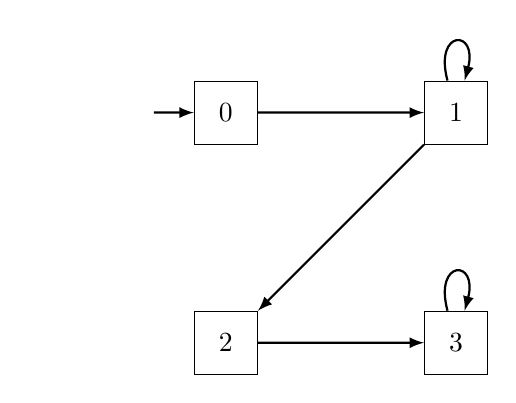
\begin{tikzpicture} [scale=2.4, every initial by arrow/.style={thick}]
		
		\newcommand{\disth}{60pt}
		\newcommand{\distv}{60pt}
		
		\node at (0,0) {};
		
%		\node [gstate,init] (s16) at (\basex,\basey) {$\state_1,\state_6$};
%		\node [gstate,right=\disth of s16] (s2369) {$\state_2,\state_3,\state_6,\state_9$};
%		\node [gstate,below=\distv of s16] (s4) {$\state_4$};
%		\node [gstate,below=\distv of s2369] (s810) {$\state_8, \state_{10}$};
		
		\node [gstate,init] (s16) at (\basex,\basey) {$0$};
		\node [gstate,right=\disth of s16] (s2369) {$1$};
		\node [gstate,below=\distv of s16] (s4) {$2$};
		\node [gstate,below=\distv of s2369] (s810) {$3$};
		
		\path [trans] (s16) edge (s2369);
		\path [trans] (s2369) edge (s4);
		\path [trans] (s4) edge (s810);
		

		
		\path [trans] (s2369) edge [loop above] (s2369);
		\path [trans] (s810) edge [loop above] (s810);
		
		
		
		%		midway, at start, near start, very near start, at end, near end, very near end
		
		
	\end{tikzpicture}
\end{document}
	\end{minipage}
	\caption{Simplified representations of \mdp (left) and the \viewN \viewdistance on it (right)}
	\label{fig:Distance}  
\end{figure}

\begin{definition}
	Let $\chgph = \chgphtuple$ be \achgphN. The \emph{reverse distance} between disjoint $\states_1, \states_2 \subseteq \states$ is the length of the shortest path to a state $\state_1 \in \states_1$ from a $\state_2 \in \states_2$. That is, if $\states_1 \cap \states_2 = \emptyset$ it is		
	\[
	\distpathrev(\chgph, \states_1, \states_2) := \min\{\lenpath(\path) \mid \path \in \pathset, \; \plast(\path) \in \states_1, \; \pfirst(\path) \in \states_2\},
	\]
	\noindent
	If $\states_1 \cap \states_2 \neq \emptyset$, it is $\distpathrev(\chgph, \states_1, \states_2) := 0$.
\end{definition}

\begin{definition}
	Let $\chgph = \chgphtuple$ be \achgphN. The \emph{reverse distance} between disjoint $\states_1, \states_2 \subseteq \states$ is the length of the shortest path from a state $\state_1 \in \states_1$ to a $\state_2 \in \states_2$ ignoring the direction of edges. That is, if $\states_1 \cap \states_2 = \emptyset$ it is		
	\[
	\distpathbi(\chgph, \states_1, \states_2) := \min\{\lenpath(\pathbi) \mid \pathbi \in \pathbiset, \; \pfirst(\pathbi) \in \states_1, \; \plast(\pathbi) \in \states_2\},
	\]
	\noindent
	If $\states_1 \cap \states_2 \neq \emptyset$, it is $\distpathbi(\chgph, \states_1, \states_2) := 0$.
\end{definition}


\redcomment{Variants of ALGORITHM which allow directinoless or only reverse traversal of the \mdpN are provided in the appendix. The respective views would utilize their returned set in the exact same way. That is, \fctdistdefault is replaced with the set of the respective algorithm and nothing else changes.}



\subsubsection{Double Directed Edges with same Action}
\redcomment{NOT SURE IF SHOULD BE INCLUDED}
\begin{definition}
	Let $\chgph = \chgphtuple$ be \achgphN.
\end{definition}

\subsubsection{Cycles}
A cycle is a structure that can exist in every graph. The concept of cycles is not specific to \chgphsN or any of its more specialized variants. The purpose of this thesis is to discuss views that utilize domain specific knowledge or if a general concept is of special relevance when exploring \achgphN. The former and the latter apply on cycles.

Formalizing \viewsN based on cycles requires some formalization of the concept cycle. We will use a domain specific definition that will serve us the most.

\begin{definition}
	Let $\chgph = \chgphtuple$ be \achgphN. A (simple) \emph{cycle} \cycle in \chgph is a sequence \cyclesecfull alternating between states and actions where $n \in \natnums, \{\state_0, \dots, \state_{n-1}\} \subseteq \states$ is a set of distinct states,  $\{\action_0, \dots, \action_{n-1}\} \subseteq \actions$ and for all $i \in \{0, \dots, n-1\}$ it is $(\state_i,\action_i, \state_{i+1 \text{ mod }n}) \in \trans$.
\end{definition}

When the actions in the cycle are of no further importance, we will omit them only writing a sequence of states. In the following let $\cycle = \cyclesecfull$ be a cycle. For conveniences we will write $\state \in \cycle$ if the state is contained in the cycle \cycle and $\action \in \cycle$ if the action is contained in in the cycle \cycle. \redcomment{only if??} In words we will both write a state or action is \emph{on} or \emph{in} the cycle. Let $\cycle_1$ and $\cycle_2$ be cycles. $\cycle_1 \cup \cycle_2 := \{\state \in \states \mid \state \in \cycle_1 \text{ or } \state \in \cycle_2\}$.

\begin{definition}
	Let \cycle be an cycle in \chgph and \states be the states set of \chgph. The number $|\{\state \in \states \mid \state \in \cycle\}| =: \lencycle(\cycle)$ is called the \emph{length} of a cycle. 
\end{definition}

\begin{definition}
	Let $\chgph$ be an \chgphN. The set $\cycleset := \{ \cycle \mid \lencycle(\cycle) \geq n\}$ declares the set of all cycles in \chgph with a length of at least $n$.
\end{definition}

In practice there exist several cycle finding algorithms. The function $\fctfindcycles(\chgph, n)$ is an abstraction for one of these algorithms being used. The actual implementation relys on algorithms of the jave library \jgrapht namely the \redcomment{Algorithm Szwarcfiter and Lauer - $O(V+EC)$ and Tiernan - $O(V.constV)$ CITATION!!}

With the formalization done we will introduce some views utilizing the concept cycles. For one we will combine the notion cycle with domain specific knowledge for the other we will consider how and why cycles in MDPs are in general of relevance. We will begin with the latter.  Cycles in general are of interest because they pose the risk of getting stuck in endless loops, when performing actions on the \mdpN. \redcomment{Model checking is one of the most relevant actions on \chgphsN that are vulnerable to loops. They are performed commonly on them.} Therefore a \viewN that simply finds existing cycles is feasible.


\begin{definition}
	Let $\chgph = \chgphtuple$ be \achgphN and $n \in \natnums$. The \viewN \viewhascycle is defined by its \grpfctN $\gfcthascycle : \states \to \imggrp$ with
	\[
	\state \mapsto
	\begin{cases}
			\group, &\text{if } \cycleset \neq \emptyset \\
			\remelem, &\text{otherwise}
		\end{cases}
	\]
	
	and $\imggrp = \{\group, \remelem\}$.
\end{definition}

This \viewN groups all states that are contained in cycle with a length of at least $n$. It is to note that the affinity of a state to one or several respective cycles is lost.

\redcomment{DISCUSSION OF EQUALITY, EQ CLASSES AND RESULTING STATES MISSING}

\begin{definition}
	Let $\chgph = \chgphtuple$ be \achgphN and $n \in \natnums$. The \viewN \viewexactcycle is defined by its \grpfctN $\gfctexactcycle : \states \to \imggrp$ with
	\[
	\state \mapsto \{\cycle \in \cycleset \mid \state \in \cycle\}
	\]
	
	and $\imggrp = \powerset{\cycleset}\cup \remset.$
	\label{def:exactcycleview}
\end{definition}

This \viewN groups states that have the same set of cycles they are contained in. Thus if $C_1$ and $C_2$ are distinct cycles and $\state_1, \state_2 \in \cycle_1$ and $\state_1 \in \cycle_2$ but $\state_2 \notin \cycle_2$ they are not grouped. It suffices that a state is on one cycle that the other one is not on, in order for the states not being grouped. In graphs with many cycles this can lead to little grouping.


\begin{figure}[h]
	\centering
	\documentclass[tikz,preview]{standalone}
%\usepackage{prelude}

%%%%%%%%%%%%%%%%%%%%%%%%%%%%%%%%%%%% PACKAGES %%%%%%%%%%%%%%%%%%%%%%%%%%%%%%%%%%%%%%%%%%

\usepackage{inputenc,fontenc}
\usepackage[a4paper,margin=3cm]{geometry}
\usepackage[english]{babel}
%\usepackage[german]{babel}
%\usepackage[fixlanguage]{babelbib}


\usepackage{bbold}
\usepackage{amsthm}
\usepackage{amsmath}
\usepackage{amssymb} % doteqdot
\usepackage[dvipsnames]{xcolor}
\usepackage{standalone}
\usepackage{tikz}[mode=buildnew]
\usepackage{cite}
\usepackage{xspace}
\usepackage{relsize}
\usepackage{mathtools} % mathclap
%\usepackage{MnSymbol}
\usepackage{hyperref}
\usepackage{url}
\usepackage{listings} % for code
\usepackage[T1]{fontenc} %<
\hypersetup{
	colorlinks,
	citecolor=black,
	filecolor=black,
	linkcolor=black,
	urlcolor=black
}
\usepackage{pgfplots}
\pgfplotsset{compat=1.18}
%\usepackage{courier} %% Sets font for listing as Courier. But also for url and texttt!
\usepackage{listings, xcolor}
\usepackage{graphicx}
\usepackage{subcaption}

\usetikzlibrary{calc}
%\usepackage{xparse} % \newDocumentCommand for multiple optional arguments
%\usepackage{titlecaps}



%%%%%%%%%%%%%%%%%%%%%%%%%%%%%%%%%%%% THEOREMSTYLES %%%%%%%%%%%%%%%%%%%%%%%%%%%%%%%%%%

\theoremstyle{definition}
\newtheorem{definition}{Definition}[section]
\newtheorem{exmp}{Beispiel}[section]
%\AfterEndEnvironment{definition}{\noindent\ignorespaces}

\theoremstyle{theorem}
\newtheorem{theorem}{Satz}[section]
\newtheorem{proposition}{Proposition}[section]
%\AfterEndEnvironment{theorem}{\noindent\ignorespaces}

\theoremstyle{korollary}
\newtheorem{korollary}{Korollar}[section]
%\AfterEndEnvironment{korollary}{\noindent\ignorespaces}


\tikzset{
	mstate/.style={draw, circle, minimum size=.94cm}, 
	gstate/.style={draw, rectangle, minimum size=.8cm},
	varstate/.style={draw,rectangle, rounded corners, minimum size=1}, 
	trans/.style={draw, ->, thick},
	bendtrans/.style={draw, ->, thick, bend left=10},
	bendtransr/.style={draw, ->, thick, bend right=10},
	init/.style={initial, initial distance=6pt, initial text=},
	every loop/.style={min distance=5pt, looseness=8},
	>=latex
}
\usetikzlibrary{automata,positioning}

%auto shift/.style={auto=right,->,
%	to path={ let \p1=(\tikztostart),\p2=(\tikztotarget),
%		\n1={atan2(\y2-\y1,\x2-\x1)},\n2={\n1+180}
%		in ($(\tikztostart.{\n1})!1mm!270:(\tikztotarget.{\n2})$) -- 
%		($(\tikztotarget.{\n2})!1mm!90:(\tikztostart.{\n1})$) \tikztonodes}},

%%%%%%%%%%%%%%%%%%%%%%%%%%%%%%%%%%% MY MACROS %%%%%%%%%%%%%%%%%%%%%%%%%%%%%%%%%%%%%%%%%
%formatting
\newcommand{\comment}[2]{{\color{#1}#2}}
\newcommand{\redcomment}[1]{{\color{red}#1}}
\newcommand{\purpcomment}[1]{{\color{pink}#1}}
\newcommand{\bluecomment}[1]{{\color{blue}#1}}
\newcommand{\mt}[1]{\ensuremath{{#1}}\xspace}
\newcommand{\mynewcommand}[2]{\newcommand{#1}{\mt{#2}}} %% currently not used becaue of ide highlighting
\newcommand{\arr}{\mt{\to}}

%model checking terms
\newcommand{\mimicrel}{\mt{\mathcal{R}}}
\newcommand{\bisimeq}{\mt{\;\!\sim\;\!}}
\newcommand{\simorder}{\mt{\;\!\preceq\;\!}}
\newcommand{\simequiv}{\mt{\;\!\simeq\;\!}} %command already defined
\newcommand{\relts}{\mt{\;\!\bullet_{_{\tiny{TS}}}\;\!}}
\newcommand{\rel}{\mt{\;\!\bullet\;\!}}

%own names
\newcommand{\nm}[1]{#1\xspace}
\newcommand{\mdpN}{\nm{MDP}}
\newcommand{\mdpsN}{\nm{MDPs}}
\newcommand{\viewN}{\nm{view}}
\newcommand{\viewNC}{\nm{View}}
\newcommand{\viewsN}{\nm{views}}
\newcommand{\viewsNC}{\nm{Views}}
\newcommand{\grpfctsubN}{\nm{detached grouping function}}
\newcommand{\grpfctsubNC}{\nm{detached grouping function}}
\newcommand{\grpfctsubNCC}{\nm{Detached Grouping Function}}
\newcommand{\grpfctN}{\nm{grouping function}}
\newcommand{\grpfctNC}{\nm{Grouping function}}
\newcommand{\grpfctNCC}{\nm{Grouping Function}}
\newcommand{\grpfctsN}{\nm{grouping functions}}
\newcommand{\grpfctsNC}{\nm{Grouping functions}}
\newcommand{\grpfctsNCC}{\nm{Grouping Functions}}
\newcommand{\stmimicN}{\nm{state-mimic}}
\newcommand{\stmimicsN}{\nm{state-mimics}}
\newcommand{\stmimickingN}{\nm{state-mimicking}}
\newcommand{\stmimickedN}{\nm{state-mimicked}}
%\newcommand{\chosenphtypeNCC}{\nm{Transition System}}
%\newcommand{\chgphNC}{\nm{Transition system}}
%\newcommand{\chgphN}{\nm{transition system}}
%\newcommand{\chgphsNCC}{\nm{Transition Systems}}
%\newcommand{\chgphsNC}{\nm{Transition systems}}
%\newcommand{\chgphsN}{\nm{transition systems}}
\newcommand{\chgphNCC}{\nm{MDP}}
\newcommand{\chgphNC}{\nm{MDP}}
\newcommand{\chgphN}{\nm{MDP}}
\newcommand{\achgphN}{\nm{an MDP}}
\newcommand{\chgphsNCC}{\nm{MDPs}}
\newcommand{\chgphsNC}{\nm{MDPs}}
\newcommand{\chgphsN}{\nm{MDPs}}
\newcommand{\parllcompN}{\nm{parallel composition}}
\newcommand{\parllcompNC}{\nm{Parallel composition}}
\newcommand{\parllcompNCC}{\nm{Parallel Composition}}
\newcommand{\parllcompsN}{\nm{parallel compositions}}
\newcommand{\parllcompsNC}{\nm{Parallel compositions}}
\newcommand{\parllcompsNCC}{\nm{Parallel Compositions}}
\newcommand{\sccN}{\nm{SCC}}
\newcommand{\sccsN}{\nm{SCCs}}
\newcommand{\bsccN}{\nm{BSCC}}
\newcommand{\bsccsN}{\nm{BSCCs}}
\newcommand{\jgrapht}{\nm{jGraphtT}}

\newcommand{\outactident}{\nm{OutActionsIdent}}

%names
\newcommand{\iffN}{\nm{if and only if}}
\newcommand{\tsN}{\nm{TS}}

%% outactions identical
\newcommand{\outactidentstrong}{\nm{strong}}
\newcommand{\outactidentweak}{\nm{weak}}

% CORE DEFINITIONS
\newcommand{\grpfct}[1][\viewppty]{\mt{F_{#1}}}
\newcommand{\grpfctsub}[1][\viewppty]{\mt{\tilde{F}_{#1}}}
%\newcommand{\grpfctimg}[1]{\mt{{\grpfct}[{#1}]}}
%\newcommand{\fctimg}[2]{\mt{{#1}[{#2}]}}
\newcommand{\eqrelview}{\mt{R}}
\newcommand{\eqclassv}[1][\state]{\mt{\eqclass{#1}{\eqrelview}}}
\newcommand{\eqclasssetv}[1][\states]{\mt{{#1}/\eqrelview}} %OLD: \bigcup_{\state \in \states} \eqclassv
\newcommand{\viewid}{\mt{\mdp}}
\newcommand{\view}[1][\viewppty]{\mt{\viewid_{#1}}}
\newcommand{\imggrp}{\mt{\arbset}}
\newcommand{\imggrpsub}{\mt{X}}
\newcommand{\viewppty}{\mt{\theta}}
\newcommand{\pll}{\mt{\;\!\pllpure\;\!}}
\newcommand{\pllrev}{\mt{\pllpure^{-1}}}
\newcommand{\pllpure}{\mt{||}}
\newcommand{\compselectset}{\mt{Z}}
\newcommand{\compselectpure}{\mt{\pllpure_\compselectset}}
\newcommand{\compselect}{\mt{\;\pllpure_\compselectset\;}}
\newcommand{\remstates}{\mt{\bigcup_{\state \in \states \setminus \states_1}\{\{\state\}\}}}
\newcommand{\nogroupstates}[1][\states_2]{\mt{\bigcup_{\state \in \states \setminus {#1}}\{\{\state\}\}}}
\newcommand{\remelem}{\mt{\bullet}}
\newcommand{\nogroupset}{\mt{\xi}}
\newcommand{\remset}{\mt{\{\remelem\}}}
\newcommand{\gfctpll}{\mt{\grpfct[\pll]}}
\newcommand{\group}{\mt{\top}}
\newcommand{\imggrpbinview}{\mt{\{\remelem, \notppty\}}}
\newcommand{\viewappset}{\mt{\tilde{\states}}}
\newcommand{\hasppty}{\mt{\top}}
\newcommand{\notppty}{\mt{\bot}}
\newcommand{\disregardelem}{\mt{\Delta}}
\newcommand{\disregardelements}{\mt{{\disregardelem_1, \dots, \disregardelem_n}}}



%\newcommand{\mdp}{def}\mdp
%\newcommand{\mdpdef}



% EXAMPLE VIEWS
\newcommand{\pptyatomicprops}{\mt{\atomicprops}}
\newcommand{\pptyinitstates}{\mt{\initstates}}
\newcommand{\pptyinactsetsize}{\mt{|\inacts(\state)|}}
\newcommand{\pptyhasoutact}{\mt{\exists\outact}}
\newcommand{\pptyminoutact}[2]{\mt{#1\leq#2}}
\newcommand{\pptymaxoutact}[2]{\mt{#2\leq#1}}
\newcommand{\pptyspanoutact}[3]{\mt{#1\leq#2\leq#3}}
\newcommand{\pptyoutactsetsize}{\mt{|\outacts(\state)|}}
\newcommand{\pptyoutactsingle}{\mt{|\outacts(\state)|_1}}
\newcommand{\pptystrongoutactident}{\mt{\outacts(\state)_=}}
\newcommand{\pptyweakoutactident}{\mt{\outacts(\state)_\approx}}
\newcommand{\pptyhasinact}{\mt{\exists\inact}}
\newcommand{\pptymininact}[2]{\mt{#1\leq#2}}
\newcommand{\pptymaxinact}[2]{\mt{#2\leq#1}}
\newcommand{\pptyspaninact}[3]{\mt{#1\leq#2\leq#3}}
\newcommand{\pptyinactsingle}{\mt{|\inacts(\state)|_1}}
\newcommand{\pptystronginactident}{\mt{\inacts(\state)_=}}
\newcommand{\pptyweakinactident}{\mt{\inacts(\state)_\approx}}
\newcommand{\pptyparamvalueseq}{\mt{\var = \varval}}
\newcommand{\pptyparamvaluesneq}{\mt{\var \neq \varval}}
\newcommand{\pptyparamdnf}{\mt{VarDNF}}
\newcommand{\pptyparamcnf}{\mt{VarCNF}}
\newcommand{\pptyparamvalueseqopt}{\mt{\var = \varval}}
\newcommand{\pptyparamvalident}{\mt{Var:\varval}}
\newcommand{\pptydistance}{\mt{\distpath}}
\newcommand{\pptydistancerev}{\mt{\distpathrev}}
\newcommand{\pptydistancebi}{\mt{\distpathbi}}
\newcommand{\pptyhascycle}{\mt{\exists\cycle}}
\newcommand{\pptyexactactcycle}{\mt{\{\cycle_{\action,n}\}}}
\newcommand{\pptycycleset}{\mt{\cup{\{\state\}_\cycle}}}
\newcommand{\pptyexactcycle}{\mt{\{\cycle_n\}}}
\newcommand{\pptyscc}{\mt{scc}}
\newcommand{\pptybscc}{\mt{bscc}}
\newcommand{\pptyprop}{\mt{\redcomment{?}}}
\newcommand{\pptyident}{id}


\newcommand{\gfctatomicprops}{\mt{\grpfct[\pptyatomicprops]}}
\newcommand{\gfctinitstates}{\mt{\grpfct[\pptyinitstates]^\hasppty}}
\newcommand{\gfcthasoutaction}{\mt{\grpfct[\pptyhasoutact]^\hasppty}}
\newcommand{\gfctminoutaction}{\mt{\grpfct[\pptyminoutact{\numoutact}{\outact}]^\hasppty}}
\newcommand{\gfctmaxoutaction}{\mt{\grpfct[\pptymaxoutact{\numoutact}{\outact}]^\hasppty}}
\newcommand{\gfctspanoutaction}{\mt{\grpfct[\pptyspanoutact{\numoutactb}{\outact}{\numoutact}]^\hasppty}}
\newcommand{\gfctoutactsetsize}{\mt{\grpfct[\pptyoutactsetsize]}}
\newcommand{\gfctoutactsingle}{\mt{\grpfct[\pptyoutactsingle]^\notppty}}
\newcommand{\gfctstrongoutactident}{\mt{\grpfct[\pptystrongoutactident]}}
\newcommand{\gfctweakoutactident}{\mt{\grpfct[\pptyweakoutactident]}}
\newcommand{\gfcthasinaction}{\mt{\grpfct[\pptyhasinact]^\hasppty}}
\newcommand{\gfctmininaction}{\mt{\grpfct[\pptymininact{\numinact}{\inact}]^\hasppty}}
\newcommand{\gfctmaxinaction}{\mt{\grpfct[\pptymaxinact{\numinact}{\inact}]^\hasppty}}
\newcommand{\gfctspaninaction}{\mt{\grpfct[\pptyspaninact{\numinactb}{\inact}{\numinact}]^\hasppty}}
\newcommand{\gfctinactsetsize}{\mt{\grpfct[\pptyinactsetsize]}}
\newcommand{\gfctinactsingle}{\mt{\grpfct[\pptyinactsingle]^\notppty}}
\newcommand{\gfctstronginactident}{\mt{\grpfct[\pptystronginactident]}}
\newcommand{\gfctweakinactident}{\mt{\grpfct[\pptyweakinactident]}}
\newcommand{\gfctparamvalueseq}{\mt{\grpfct[\pptyparamvalueseq]^\hasppty}}
\newcommand{\gfctparamvaluesneq}{\mt{\grpfct[\pptyparamvaluesneq]^\hasppty}}
\newcommand{\gfctparamdnf}{\mt{\grpfct[\pptyparamdnf]^\hasppty}}
\newcommand{\gfctparamcnf}{\mt{\grpfct[\pptyparamcnf]^\hasppty}}
\newcommand{\gfctparamvalueseqopt}{\mt{\pptyparamvalueseqopt}}
\newcommand{\gfctparamvalident}{\mt{\grpfct[\pptyparamvalident]}}
\newcommand{\gfctdistance}{\mt{\grpfct[\pptydistance]}}
\newcommand{\gfctdistancerev}{\mt{\grpfct[\pptydistancerev]}}
\newcommand{\gfctdistancebi}{\mt{\grpfct[\pptydistancebi]}}
\newcommand{\gfcthascycle}{\mt{\grpfct[\pptyhascycle]}}
\newcommand{\gfctexactcycle}{\mt{\grpfct[\pptyexactcycle]}}
\newcommand{\gfctcycleset}{\mt{\grpfct[\pptycycleset]}}
\newcommand{\gfctexactactcycle}{\mt{\grpfct[\pptyexactactcycle]}}
\newcommand{\gfctscc}{\mt{\grpfct[\pptyscc]}}
\newcommand{\gfctbscc}{\mt{\grpfct[\pptybscc]}}
\newcommand{\gfctprop}{\mt{\grpfct[\pptyprop]}}
\newcommand{\gfctident}{\mt{\grpfct[\pptyident]}}

\newcommand{\gfctsubatomicprops}{\mt{\grpfctsub[\pptyatomicprops]}}
\newcommand{\gfctsubinitstates}{\mt{\grpfctsub[\pptyinitstates]^\hasppty}}
\newcommand{\gfctsubhasoutaction}{\mt{\grpfctsub[\pptyhasoutact]^\hasppty}}
\newcommand{\gfctsubminoutaction}{\mt{\grpfctsub[\pptyminoutact{\numoutact}{\outact}]^\hasppty}}
\newcommand{\gfctsubmaxoutaction}{\mt{\grpfctsub[\pptymaxoutact{\numoutact}{\outact}]^\hasppty}}
\newcommand{\gfctsubspanoutaction}{\mt{\grpfctsub[\pptyspanoutact{\numoutactb}{\outact}{\numoutact}]^\hasppty}}
\newcommand{\gfctsuboutactsetsize}{\mt{\grpfctsub[\pptyoutactsetsize]}}
\newcommand{\gfctsuboutactsingle}{\mt{\grpfctsub[\pptyoutactsingle]^\notppty}}
\newcommand{\gfctsubstrongoutactident}{\mt{\grpfctsub[\pptystrongoutactident]^\hasppty}}
\newcommand{\gfctsubweakoutactident}{\mt{\grpfctsub[\pptyweakoutactident]^\hasppty}}
\newcommand{\gfctsubhasinaction}{\mt{\grpfctsub[\pptyhasinact]}}
\newcommand{\gfctsubmininaction}{\mt{\grpfctsub[\pptymininact{\numinact}{\inact}]}}
\newcommand{\gfctsubmaxinaction}{\mt{\grpfctsub[\pptymaxinact{\numinact}{\inact}]}}
\newcommand{\gfctsubspaninaction}{\mt{\grpfctsub[\pptyspaninact{\numinactb}{\inact}{\numinact}]}}
\newcommand{\gfctsubinactsetsize}{\mt{\grpfctsub[\pptyinactsetsize]^\hasppty}}
\newcommand{\gfctsubinactsingle}{\mt{\grpfctsub[\pptyinactsingle]^\notppty}}
\newcommand{\gfctsubstronginactident}{\mt{\grpfctsub[\pptystronginactident]}}
\newcommand{\gfctsubweakinactident}{\mt{\grpfctsub[\pptyweakinactident]}}
\newcommand{\gfctsubparamvalueseq}{\mt{\grpfctsub[\pptyparamvalueseq]^\hasppty}}
\newcommand{\gfctsubparamvaluesneq}{\mt{\grpfctsub[\pptyparamvaluesneq]^\hasppty}}
\newcommand{\gfctsubparamdnf}{\mt{\grpfctsub[\pptyparamdnf]^\hasppty}}
\newcommand{\gfctsubparamcnf}{\mt{\grpfctsub[\pptyparamcnf]^\hasppty}}
\newcommand{\gfctsubparamvalueseqopt}{\mt{\pptyparamvalueseqopt}}
\newcommand{\gfctsubparamvalident}{\mt{\grpfctsub[\pptyparamvalident]}}
\newcommand{\gfctsubdistance}{\mt{\grpfctsub[\pptydistance]}}
\newcommand{\gfctsubdistancerev}{\mt{\grpfctsub[\pptydistancerev]}}
\newcommand{\gfctsubdistancebi}{\mt{\grpfctsub[\pptydistancebi]}}
\newcommand{\gfctsubhascycle}{\mt{\grpfctsub[\pptyhascycle]^\hasppty}}
\newcommand{\gfctsubexactcycle}{\mt{\grpfctsub[\pptyexactcycle]}}
\newcommand{\gfctsubcycleset}{\mt{\grpfctsub[\pptycycleset]}}
\newcommand{\gfctsubexactactcycle}{\mt{\grpfctsub[\pptyexactactcycle]}}
\newcommand{\gfctsubscc}{\mt{\grpfctsub[\pptyscc]}}
\newcommand{\gfctsubbscc}{\mt{\grpfctsub[\pptybscc]}}
\newcommand{\gfctsubprop}{\mt{\grpfctsub[\pptyprop]}}
\newcommand{\gfctsubident}{\mt{\grpfctsub[\pptyident]}}


\newcommand{\viewatomicprops}{\mt{\view[\pptyatomicprops]}}
\newcommand{\viewinitstates}{\mt{\view[\pptyinitstates]^\hasppty}}
\newcommand{\viewhasoutaction}{\mt{\view[\pptyhasoutact]^\hasppty}}
\newcommand{\viewminoutaction}{\mt{\view[\pptyminoutact{\numoutact}{\outact}]^\hasppty}}
\newcommand{\viewmaxoutaction}{\mt{\view[\pptymaxoutact{\numoutact}{\outact}]^\hasppty}}
\newcommand{\viewspanoutaction}{\mt{\view[\pptyspanoutact{\numoutactb}{\outact}{\numoutact}]^\hasppty}}
\newcommand{\viewoutactsetsize}{\mt{\view[\pptyoutactsetsize]}}
\newcommand{\viewoutactsingle}{\mt{\view[\pptyoutactsingle]^\notppty}}
\newcommand{\viewstrongoutactident}{\mt{\view[\pptystrongoutactident]}}
\newcommand{\viewweakoutactident}{\mt{\view[\pptyweakoutactident]}}
\newcommand{\viewhasinaction}{\mt{\view[\pptyhasinact]^\hasppty}}
\newcommand{\viewmininaction}{\mt{\view[\pptymininact{\numinact}{\inact}]^\hasppty}}
\newcommand{\viewmaxinaction}{\mt{\view[\pptymaxinact{\numinact}{\inact}]^\hasppty}}
\newcommand{\viewspaninaction}{\mt{\view[\pptyspaninact{\numinactb}{\inact}{\numinact}]^\hasppty}}
\newcommand{\viewinactsetsize}{\mt{\view[\pptyinactsetsize]}}
\newcommand{\viewinactsingle}{\mt{\view[\pptyinactsingle]^\notppty}}
\newcommand{\viewstronginactident}{\mt{\view[\pptystronginactident]}}
\newcommand{\viewweakinactident}{\mt{\view[\pptyweakinactident]}}
\newcommand{\viewparamvalueseq}{\mt{\view[\pptyparamvalueseq]}}
\newcommand{\viewparamvaluesneq}{\mt{\view[\pptyparamvaluesneq]}}
\newcommand{\viewparamdnf}{\mt{\view[\pptyparamdnf]^\hasppty}}
\newcommand{\viewparamcnf}{\mt{\view[\pptyparamcnf]^\hasppty}}
\newcommand{\viewparamvalueseqopt}{\mt{\pptyparamvalueseqopt}}
\newcommand{\viewparamvalident}{\mt{\view[\pptyparamvalident]}}
\newcommand{\viewdistance}{\mt{\view[\pptydistance]}}
\newcommand{\viewdistancerev}{\mt{\view[\pptydistancerev]}}
\newcommand{\viewdistancebi}{\mt{\view[\pptydistancebi]}}
\newcommand{\viewhascycle}{\mt{\view[\pptyhascycle]}}
\newcommand{\viewexactcycle}{\mt{\view[\pptyexactcycle]}}
\newcommand{\viewcycleset}{\mt{\view[\pptycycleset]}}
\newcommand{\viewexactactcycle}{\mt{\view[\pptyexactactcycle]}}
\newcommand{\viewscc}{\mt{\view[\pptyscc]}}
\newcommand{\viewbscc}{\mt{\view[\pptybscc]}}
\newcommand{\viewprop}{\mt{\view[\pptyprop]}}
\newcommand{\viewident}{\mt{\view[\pptyident]}}

%\newcommand{\viewatomicprops}{\mt{\view[\atomicprops]}}
%\newcommand{\viewinitstates}{\mt{\view[\initstates]}}
%\newcommand{\viewhasoutaction}{\mt{\view[\pptyhasoutact]}}
%\newcommand{\viewminoutaction}{\mt{\view[\pptyminoutact{\numoutact}{\outact}]}}
%\newcommand{\viewmaxoutaction}{\mt{\view[\pptymaxoutact{\numoutact}{\outact}]}}
%\newcommand{\viewspanoutaction}{\mt{\view[\pptyspanoutact{\numoutactb}{\outact}{\numoutact}]}}
%\newcommand{\viewoutactsetsize}{\mt{\view[\pptyoutactsetsize]}}
%\newcommand{\viewoutactsingle}{\mt{\view[\pptyoutactsingle]}}
%\newcommand{\viewstrongoutactident}{\mt{\view[\outacts(\state)_=]}}
%\newcommand{\viewweakoutactident}{\mt{\view[\outacts(\state)_\approx]}}
%\newcommand{\viewhasinaction}{\mt{\view[\pptyhasinact]}}
%\newcommand{\viewmininaction}{\mt{\view[\pptymininact{\numinact}{\inact}]}}
%\newcommand{\viewmaxinaction}{\mt{\view[\pptymaxinact{\numinact}{\inact}]}}
%\newcommand{\viewspaninaction}{\mt{\view[\pptyspaninact{\numinactb}{\inact}{\numinact}]}}
%\newcommand{\viewinactsetsize}{\mt{\view[\pptyinactsetsize]}}
%\newcommand{\viewinactsingle}{\mt{\view[\pptyinactsingle]}}
%\newcommand{\viewstronginactident}{\mt{\view[\inacts(\state)_=]}}
%\newcommand{\viewweakinactident}{\mt{\view[\inacts(\state)_\approx]}}
%\newcommand{\viewparamvalueseq}{\mt{\view[\var = \varval]}}
%\newcommand{\viewparamvaluesneq}{\mt{\view[\var \neq \varval]}}
%\newcommand{\viewparamdnf}{\mt{\view[VarDNF]}}
%\newcommand{\viewparamcnf}{\mt{\view[VarCNF]}}
%\newcommand{\viewparamvalident}{\mt{\view[\pptyparamvalident]}}
%\newcommand{\viewdistance}{\mt{\view[\pptydistance]}}
%\newcommand{\viewhascycle}{\mt{\view[\exists\cycle]}}
%\newcommand{\viewexactcycle}{\mt{\view[\pptyexactcycle]}}
%\newcommand{\viewcycleset}{\mt{\view[\pptycycleset]}}
%\newcommand{\viewexactactcycle}{\mt{\view[\pptyexactactcycle]}}
%\newcommand{\viewscc}{\mt{\view[scc]}}
%\newcommand{\viewbscc}{\mt{\view[bscc]}}

%actions
\newcommand{\numoutact}{\mt{n}}
\newcommand{\numoutactb}{\mt{m}}
\newcommand{\numinact}{\mt{n}}
\newcommand{\numinactb}{\mt{m}}

\newcommand{\predmaxoutact}[1][\numoutact]{\mt{Q_{\outact\leq#1}(\state,\state_1, \dots, \state_{#1+1})}}
\newcommand{\predminoutact}[1][\numoutact]{\mt{Q_{#1\leq\outact}(\state,\state_1, \dots, \state_{#1})}}
\newcommand{\formoutact}[1][\state]{\mt{C_{#1,\outact}}}
\newcommand{\predmaxinact}[1][\numinact]{\mt{Q_{\inact\leq#1}(\state,\state_1, \dots, \state_{#1+1})}}
\newcommand{\predmininact}[1][\numinact]{\mt{Q_{#1\leq\inact}(\state,\state_1, \dots, \state_{#1})}}

\newcommand{\outact}[1][\action]{\mt{\overrightarrow{#1}}}
\newcommand{\outacts}{\mt{\overrightarrow{\actions}}}
\newcommand{\inact}{\mt{\overleftarrow{\action}}}
\newcommand{\inacts}[1][\action]{\mt{\overleftarrow{#1}}}

%%Parameters
\newcommand{\vars}[1][\mdp]{\mt{V\!ar_{#1}}}
\newcommand{\var}{\mt{x}}
\newcommand{\varstate}[1][]{\mt{\var_{\state#1}}}
\newcommand{\varval}{\mt{a}}
\newcommand{\vareval}[1][\mdp]{\mt{V\!arEval_{#1}}}
\newcommand{\varevalimg}[1][\mdp]{\mt{\vareval[#1][\states,\vars]}}
\newcommand{\varevalimgset}{\mt{\arbset}}
\newcommand{\someparam}{\mt{\tilde{x}}}
\newcommand{\eqorneq}{\mt{\;\doteqdot\;}}
\newcommand{\varstyle}[2]{\mt{\langle#1,#2\rangle}}




%\makeatletter
%\newcommand{\overleftrightsmallarrow}{\mathpalette{\overarrowsmall@\leftrightarrowfill@}}
%\newcommand{\overrightsmallarrow}{\mathpalette{\overarrowsmall@\rightarrowfill@}}
%\newcommand{\overleftsmallarrow}{\mathpalette{\overarrowsmall@\leftarrowfill@}}
%\newcommand{\overarrowsmall@}[3]{%
%	\vbox{%
%		\ialign{%
%			##\crcr
%			#1{\smaller@style{#2}}\crcr
%			\noalign{\nointerlineskip}%
%			$\m@th\hfil#2#3\hfil$\crcr
%		}%
%	}%
%}
%\def\smaller@style#1{%
%	\ifx#1\displaystyle\scriptstyle\else
%	\ifx#1\textstyle\scriptstyle\else
%	\scriptscriptstyle
%	\fi
%	\fi
%}
%\makeatother
%\newcommand{\te}[1]{\overleftrightsmallarrow{#1}}

% Distance
\newcommand{\fctdist}{\mt{distance}}
\newcommand{\fctdistdefault}{\mt{\fctdist(\chgph, \smstates, \grandist)}}
\newcommand{\distval}{\mt{d}}
\newcommand{\grandist}{\mt{n}}
\let\path\oldpath
\newcommand{\path}{\mt{P}}
\newcommand{\pathbi}{\mt{\bar{\path}}}
\newcommand{\pathsecfull}{\mt{(\state_0, \action_0, \state_1, \action_1, \dots, \action_{n}, \state_{n+1})}}
\newcommand{\lenpath}{\mt{len}}
\newcommand{\pfirst}{\mt{first}}
\newcommand{\plast}{\mt{last}}
\newcommand{\pathset}{\mt{\path_\chgph}}
\newcommand{\pathbiset}{\mt{\pathbi_\chgph}}
\newcommand{\distpath}{\mt{\overrightarrow{dist}}}
\newcommand{\distpathrev}{\mt{\overleftarrow{dist}}}
\newcommand{\distpathbi}{\mt{\overline{dist}}}
%Cycles
\newcommand{\cyclesecfull}{\mt{(\state_0, \action_0, \state_1, \action_1, \dots, \action_{n-1}, \state_0)}}
\newcommand{\fctfindcycles}{\mt{findCycles}}
\newcommand{\cycle}{\mt{C}}
\newcommand{\cycleset}{\mt{\cycle_{\mdp, n}}}
\newcommand{\lencycle}{\mt{len}}
% strongly connected components
\newcommand{\scc}{\mt{T}}
\newcommand{\setscc}{\mt{SCC_{\chgph,n}}}
\newcommand{\setbscc}{\mt{BSCC_{\chgph,n}}}

% properties
\newcommand{\propfct}{\mt{f}}

% all Systems
\newcommand{\chgph}{\mt{\mdp}}
\newcommand{\chgphtuple}{\mt{\mdptuple}}
\newcommand{\chgphtupledist}{\mt{\mdptupledist}}

\newcommand{\states}{\mt{S}}
\newcommand{\actions}{\mt{Act}}
\newcommand{\atomicprops}{\mt{AP}}
\newcommand{\labelingfct}{\mt{L}}
\newcommand{\init}{\mt{\initdistrib}} % use MDP % refers to the underlying set
\newcommand{\trans}{\mt{\probtfunc}} % use MDP % refers to the underlying set
\newcommand{\smstates}{\mt{\tilde{\states}}}


\newcommand{\state}{\mt{s}}
\newcommand{\action}{\mt{\alpha}}
\newcommand{\actionb}{\mt{\beta}}
\newcommand{\actionc}{\mt{\gamma}}
\newcommand{\smstate}{\mt{\tilde{\state}}}



% transition sysstems
\newcommand{\ts}{\mt{TS}}
\newcommand{\transitionrel}{\mt{\longrightarrow}}
\newcommand{\initstates}{\mt{I}}
\newcommand{\transitionsystem}{\mt
	{(\states, \actions, \transitionrel, \initstates, \atomicprops, \labelingfct)}
}
\newcommand{\tstupledist}{\mt{(\states', \actions',\transitionrel', \initstates', \labelingfct')}}


%Markov chains and MDP
\newcommand{\mdp}{\mt{\autm}}
\newcommand{\mdptuple}{\mt{(\states, \actions, \probtfunc, \initdistrib, \atomicprops, \labelingfct)}}
\newcommand{\mdptupledist}{\mt{(\states', \actions', \probtfunc', \initdistrib', \atomicprops', \labelingfct')}}
\newcommand{\autm}{\mt{\mathcal{M}}}
\newcommand{\probtfunc}{\mt{\textbf{P}}}
\newcommand{\initdistrib}{\mt{\iota_{init}}}


%maths
\newcommand{\powerset}[1]{\mt{\mathcal{P}(#1)}}
\newcommand{\eqclass}[2]{\mt{[#1]_{#2}}}%{\mt{#1 / #2}}
\newcommand{\impr}{\mt{\hspace{3mm}\Rightarrow\hspace{2mm}}}
\newcommand{\impl}{\mt{\hspace{3mm}\Leftarrow\hspace{2mm}}}
\newcommand{\natnums}{\mt{\mathbb{N}}} 
\newcommand{\realnums}{\mt{\mathbb{R}}}
\newcommand{\intmodn}[1][n]{\mt{\mathbb{Z}_{#1}}}
\newcommand{\arbset}{\mt{M}}
\newcommand{\bigsum}[2][]{\mt{\mathlarger{\sum}_{#2}^{#1}}}
\newcommand{\bbigsum}[2][]{\mt{\mathlarger{\mathlarger{\sum}}_{#2}^{#1}}}
\newcommand{\invimage}[2]{#1^{\mt{-1}(#2)}}
\newcommand{\img}{\mt{Img}}
\newcommand{\cond}{\mt{\,|\,}}

%tickz
%% \definecolor{darkred}{RGB}{196, 42, 42}

%implementation
\newcommand{\pmcvis}{\nm{PMC-Vis}}


\usepackage{tikz}


\begin{document}
	\newcommand{\createstate}[3]{\node[draw, circle, minimum size=1cm] (#1) at (#2) {#3}}
	\newcommand{\basex}{0}
	\newcommand{\basey}{0}
	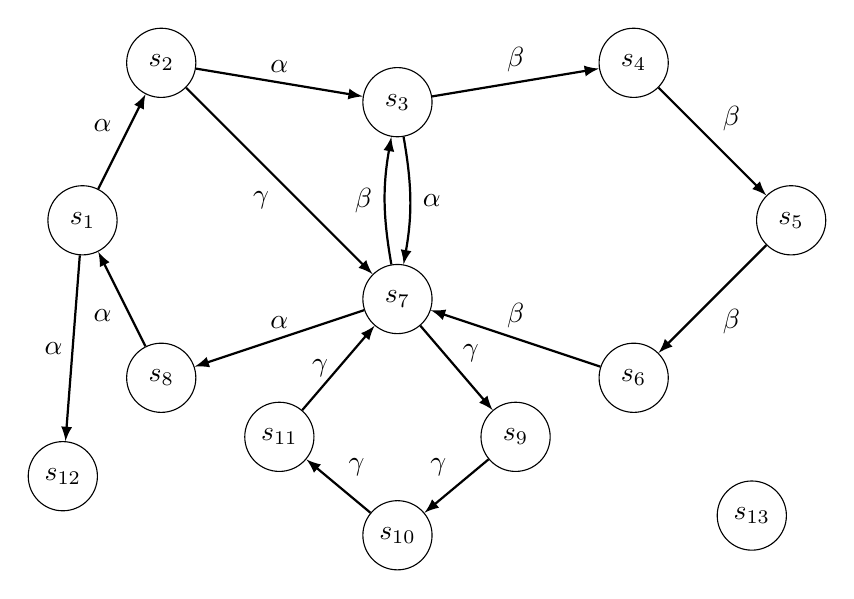
\begin{tikzpicture} [ >=latex]
		%		\createstate{s1}{3,2+4}{$\state_1$};
		\path
		(\basex,		\basey+2) 		node[state] (s1) 	{$\state_1$} 
		(\basex+2,		\basey+4) 		node[state] (s2) 	{$\state_2$} 
		(\basex+5,		\basey+3.5) 	node[state] (s3) 	{$\state_3$} 
		(\basex+8,		\basey+4) 		node[state] (s4) 	{$\state_4$}
		(\basex+10,		\basey+2) 		node[state] (s5) 	{$\state_5$}
		(\basex+8,		\basey+0) 		node[state] (s6) 	{$\state_6$}
		(\basex+5,		\basey+1) 		node[state] (s7) 	{$\state_7$}
		(\basex+2,		\basey+0) 		node[state] (s8) 	{$\state_8$}
		(\basex+6.5,	\basey-.75)		node[state] (s9) 	{$\state_9$}
		(\basex+5,		\basey-2) 		node[state] (s10) 	{$\state_{10}$}
		(\basex+3.5,	\basey-.75)		node[state] (s11) 	{$\state_{11}$}
		(\basex+.75,	\basey-1.25)	node[state] (s12) 	{$\state_{12}$}
		(\basex+9.5,	\basey-1.75)	node[state] (s13) 	{$\state_{13}$}
		;
		
		\path [trans] (s1) 	edge node [midway,above left]{\action} 		(s2);
		\path [trans] (s2) 	edge node [midway,above]{\action} 			(s3);
		\path [trans] (s3) 	edge node [midway,above]{\actionb} 			(s4);
		\path [trans] (s4) 	edge node [midway,above right]{\actionb} 	(s5);
		\path [trans] (s5)	edge node [midway,below right]{\actionb} 	(s6);
		\path [trans] (s6) 	edge node [midway,above]{\actionb} 			(s7);
		\path [trans] (s7)	edge node [midway,above]{\action} 			(s8);
		\path [trans] (s8) 	edge node [midway,below left]{\action} 			(s1);
		\path [trans] (s7) 	edge node [midway,above right=-2pt]{\actionc} 	(s9);
		\path [trans] (s9) 	edge node [midway,above left]{\actionc} 	(s10);
		\path [trans] (s10)	edge node [midway,above right]{\actionc} 	(s11);
		\path [trans] (s11)	edge node [midway,left]{\actionc} 			(s7);
		\path [trans] (s1)	edge node [midway,left]{\action} 			(s12);
		\path [trans] (s2)	edge node [midway,below left]{\actionc} 	(s7);

		\path [bendtrans] (s3) edge node [midway,left=10pt]{\actionb} (s7);
		\path [bendtrans] (s7) edge node [midway,right=10pt]{\action} (s3);
		
%		\path [trans] (s-1) -- (s-2) node [midway, above] () {\action}
		
%		(\basex+3,	\basey+1) node[state] (s-bot) {$\bot$}
%		(s-1)++(-1.2,0) node (s-1-in) {}
%		(s-3)++(-1.2,0) node (s-3-in) {};
		
		
		%		midway, at start, near start, very near start, at end, near end, very near end
		
%		\path [trans] (s-1) -- (s-bot);
%		\path [trans] (s-3) -- (s-bot);
%		\path [trans] (s-1-in) -- (s-1);
%		\path [trans] (s-3-in) -- (s-3);
		
		
	\end{tikzpicture}
\end{document}			
	\caption{Simplified representation of \mdp}
	\label{fig:cyclesBefore}  
\end{figure}



\redcomment{DISCUSSION OF EQUALITY, EQ CLASSES AND RESULTING STATES MISSING}

\redcomment{GREEDY APPROACHES (STATE ON SINGLE CYCLE), AND SET APPROACH s $\to$ $C_1 \cup C_2$ omitted because not sure if needed}

The view above might be useful when having found cycles to see what cycles specifically exist. Often it is interesting to find cycles that consist only of transitions of the same action. The following view accomplishes that.

\begin{figure}[h]
	\centering
	\documentclass[tikz,preview]{standalone}
%\usepackage{prelude}

%%%%%%%%%%%%%%%%%%%%%%%%%%%%%%%%%%%% PACKAGES %%%%%%%%%%%%%%%%%%%%%%%%%%%%%%%%%%%%%%%%%%

\usepackage{inputenc,fontenc}
\usepackage[a4paper,margin=3cm]{geometry}
\usepackage[english]{babel}
%\usepackage[german]{babel}
%\usepackage[fixlanguage]{babelbib}


\usepackage{bbold}
\usepackage{amsthm}
\usepackage{amsmath}
\usepackage{amssymb} % doteqdot
\usepackage[dvipsnames]{xcolor}
\usepackage{standalone}
\usepackage{tikz}[mode=buildnew]
\usepackage{cite}
\usepackage{xspace}
\usepackage{relsize}
\usepackage{mathtools} % mathclap
%\usepackage{MnSymbol}
\usepackage{hyperref}
\usepackage{url}
\usepackage{listings} % for code
\usepackage[T1]{fontenc} %<
\hypersetup{
	colorlinks,
	citecolor=black,
	filecolor=black,
	linkcolor=black,
	urlcolor=black
}
\usepackage{pgfplots}
\pgfplotsset{compat=1.18}
%\usepackage{courier} %% Sets font for listing as Courier. But also for url and texttt!
\usepackage{listings, xcolor}
\usepackage{graphicx}
\usepackage{subcaption}

\usetikzlibrary{calc}
%\usepackage{xparse} % \newDocumentCommand for multiple optional arguments
%\usepackage{titlecaps}



%%%%%%%%%%%%%%%%%%%%%%%%%%%%%%%%%%%% THEOREMSTYLES %%%%%%%%%%%%%%%%%%%%%%%%%%%%%%%%%%

\theoremstyle{definition}
\newtheorem{definition}{Definition}[section]
\newtheorem{exmp}{Beispiel}[section]
%\AfterEndEnvironment{definition}{\noindent\ignorespaces}

\theoremstyle{theorem}
\newtheorem{theorem}{Satz}[section]
\newtheorem{proposition}{Proposition}[section]
%\AfterEndEnvironment{theorem}{\noindent\ignorespaces}

\theoremstyle{korollary}
\newtheorem{korollary}{Korollar}[section]
%\AfterEndEnvironment{korollary}{\noindent\ignorespaces}


\tikzset{
	mstate/.style={draw, circle, minimum size=.94cm}, 
	gstate/.style={draw, rectangle, minimum size=.8cm},
	varstate/.style={draw,rectangle, rounded corners, minimum size=1}, 
	trans/.style={draw, ->, thick},
	bendtrans/.style={draw, ->, thick, bend left=10},
	bendtransr/.style={draw, ->, thick, bend right=10},
	init/.style={initial, initial distance=6pt, initial text=},
	every loop/.style={min distance=5pt, looseness=8},
	>=latex
}
\usetikzlibrary{automata,positioning}

%auto shift/.style={auto=right,->,
%	to path={ let \p1=(\tikztostart),\p2=(\tikztotarget),
%		\n1={atan2(\y2-\y1,\x2-\x1)},\n2={\n1+180}
%		in ($(\tikztostart.{\n1})!1mm!270:(\tikztotarget.{\n2})$) -- 
%		($(\tikztotarget.{\n2})!1mm!90:(\tikztostart.{\n1})$) \tikztonodes}},

%%%%%%%%%%%%%%%%%%%%%%%%%%%%%%%%%%% MY MACROS %%%%%%%%%%%%%%%%%%%%%%%%%%%%%%%%%%%%%%%%%
%formatting
\newcommand{\comment}[2]{{\color{#1}#2}}
\newcommand{\redcomment}[1]{{\color{red}#1}}
\newcommand{\purpcomment}[1]{{\color{pink}#1}}
\newcommand{\bluecomment}[1]{{\color{blue}#1}}
\newcommand{\mt}[1]{\ensuremath{{#1}}\xspace}
\newcommand{\mynewcommand}[2]{\newcommand{#1}{\mt{#2}}} %% currently not used becaue of ide highlighting
\newcommand{\arr}{\mt{\to}}

%model checking terms
\newcommand{\mimicrel}{\mt{\mathcal{R}}}
\newcommand{\bisimeq}{\mt{\;\!\sim\;\!}}
\newcommand{\simorder}{\mt{\;\!\preceq\;\!}}
\newcommand{\simequiv}{\mt{\;\!\simeq\;\!}} %command already defined
\newcommand{\relts}{\mt{\;\!\bullet_{_{\tiny{TS}}}\;\!}}
\newcommand{\rel}{\mt{\;\!\bullet\;\!}}

%own names
\newcommand{\nm}[1]{#1\xspace}
\newcommand{\mdpN}{\nm{MDP}}
\newcommand{\mdpsN}{\nm{MDPs}}
\newcommand{\viewN}{\nm{view}}
\newcommand{\viewNC}{\nm{View}}
\newcommand{\viewsN}{\nm{views}}
\newcommand{\viewsNC}{\nm{Views}}
\newcommand{\grpfctsubN}{\nm{detached grouping function}}
\newcommand{\grpfctsubNC}{\nm{detached grouping function}}
\newcommand{\grpfctsubNCC}{\nm{Detached Grouping Function}}
\newcommand{\grpfctN}{\nm{grouping function}}
\newcommand{\grpfctNC}{\nm{Grouping function}}
\newcommand{\grpfctNCC}{\nm{Grouping Function}}
\newcommand{\grpfctsN}{\nm{grouping functions}}
\newcommand{\grpfctsNC}{\nm{Grouping functions}}
\newcommand{\grpfctsNCC}{\nm{Grouping Functions}}
\newcommand{\stmimicN}{\nm{state-mimic}}
\newcommand{\stmimicsN}{\nm{state-mimics}}
\newcommand{\stmimickingN}{\nm{state-mimicking}}
\newcommand{\stmimickedN}{\nm{state-mimicked}}
%\newcommand{\chosenphtypeNCC}{\nm{Transition System}}
%\newcommand{\chgphNC}{\nm{Transition system}}
%\newcommand{\chgphN}{\nm{transition system}}
%\newcommand{\chgphsNCC}{\nm{Transition Systems}}
%\newcommand{\chgphsNC}{\nm{Transition systems}}
%\newcommand{\chgphsN}{\nm{transition systems}}
\newcommand{\chgphNCC}{\nm{MDP}}
\newcommand{\chgphNC}{\nm{MDP}}
\newcommand{\chgphN}{\nm{MDP}}
\newcommand{\achgphN}{\nm{an MDP}}
\newcommand{\chgphsNCC}{\nm{MDPs}}
\newcommand{\chgphsNC}{\nm{MDPs}}
\newcommand{\chgphsN}{\nm{MDPs}}
\newcommand{\parllcompN}{\nm{parallel composition}}
\newcommand{\parllcompNC}{\nm{Parallel composition}}
\newcommand{\parllcompNCC}{\nm{Parallel Composition}}
\newcommand{\parllcompsN}{\nm{parallel compositions}}
\newcommand{\parllcompsNC}{\nm{Parallel compositions}}
\newcommand{\parllcompsNCC}{\nm{Parallel Compositions}}
\newcommand{\sccN}{\nm{SCC}}
\newcommand{\sccsN}{\nm{SCCs}}
\newcommand{\bsccN}{\nm{BSCC}}
\newcommand{\bsccsN}{\nm{BSCCs}}
\newcommand{\jgrapht}{\nm{jGraphtT}}

\newcommand{\outactident}{\nm{OutActionsIdent}}

%names
\newcommand{\iffN}{\nm{if and only if}}
\newcommand{\tsN}{\nm{TS}}

%% outactions identical
\newcommand{\outactidentstrong}{\nm{strong}}
\newcommand{\outactidentweak}{\nm{weak}}

% CORE DEFINITIONS
\newcommand{\grpfct}[1][\viewppty]{\mt{F_{#1}}}
\newcommand{\grpfctsub}[1][\viewppty]{\mt{\tilde{F}_{#1}}}
%\newcommand{\grpfctimg}[1]{\mt{{\grpfct}[{#1}]}}
%\newcommand{\fctimg}[2]{\mt{{#1}[{#2}]}}
\newcommand{\eqrelview}{\mt{R}}
\newcommand{\eqclassv}[1][\state]{\mt{\eqclass{#1}{\eqrelview}}}
\newcommand{\eqclasssetv}[1][\states]{\mt{{#1}/\eqrelview}} %OLD: \bigcup_{\state \in \states} \eqclassv
\newcommand{\viewid}{\mt{\mdp}}
\newcommand{\view}[1][\viewppty]{\mt{\viewid_{#1}}}
\newcommand{\imggrp}{\mt{\arbset}}
\newcommand{\imggrpsub}{\mt{X}}
\newcommand{\viewppty}{\mt{\theta}}
\newcommand{\pll}{\mt{\;\!\pllpure\;\!}}
\newcommand{\pllrev}{\mt{\pllpure^{-1}}}
\newcommand{\pllpure}{\mt{||}}
\newcommand{\compselectset}{\mt{Z}}
\newcommand{\compselectpure}{\mt{\pllpure_\compselectset}}
\newcommand{\compselect}{\mt{\;\pllpure_\compselectset\;}}
\newcommand{\remstates}{\mt{\bigcup_{\state \in \states \setminus \states_1}\{\{\state\}\}}}
\newcommand{\nogroupstates}[1][\states_2]{\mt{\bigcup_{\state \in \states \setminus {#1}}\{\{\state\}\}}}
\newcommand{\remelem}{\mt{\bullet}}
\newcommand{\nogroupset}{\mt{\xi}}
\newcommand{\remset}{\mt{\{\remelem\}}}
\newcommand{\gfctpll}{\mt{\grpfct[\pll]}}
\newcommand{\group}{\mt{\top}}
\newcommand{\imggrpbinview}{\mt{\{\remelem, \notppty\}}}
\newcommand{\viewappset}{\mt{\tilde{\states}}}
\newcommand{\hasppty}{\mt{\top}}
\newcommand{\notppty}{\mt{\bot}}
\newcommand{\disregardelem}{\mt{\Delta}}
\newcommand{\disregardelements}{\mt{{\disregardelem_1, \dots, \disregardelem_n}}}



%\newcommand{\mdp}{def}\mdp
%\newcommand{\mdpdef}



% EXAMPLE VIEWS
\newcommand{\pptyatomicprops}{\mt{\atomicprops}}
\newcommand{\pptyinitstates}{\mt{\initstates}}
\newcommand{\pptyinactsetsize}{\mt{|\inacts(\state)|}}
\newcommand{\pptyhasoutact}{\mt{\exists\outact}}
\newcommand{\pptyminoutact}[2]{\mt{#1\leq#2}}
\newcommand{\pptymaxoutact}[2]{\mt{#2\leq#1}}
\newcommand{\pptyspanoutact}[3]{\mt{#1\leq#2\leq#3}}
\newcommand{\pptyoutactsetsize}{\mt{|\outacts(\state)|}}
\newcommand{\pptyoutactsingle}{\mt{|\outacts(\state)|_1}}
\newcommand{\pptystrongoutactident}{\mt{\outacts(\state)_=}}
\newcommand{\pptyweakoutactident}{\mt{\outacts(\state)_\approx}}
\newcommand{\pptyhasinact}{\mt{\exists\inact}}
\newcommand{\pptymininact}[2]{\mt{#1\leq#2}}
\newcommand{\pptymaxinact}[2]{\mt{#2\leq#1}}
\newcommand{\pptyspaninact}[3]{\mt{#1\leq#2\leq#3}}
\newcommand{\pptyinactsingle}{\mt{|\inacts(\state)|_1}}
\newcommand{\pptystronginactident}{\mt{\inacts(\state)_=}}
\newcommand{\pptyweakinactident}{\mt{\inacts(\state)_\approx}}
\newcommand{\pptyparamvalueseq}{\mt{\var = \varval}}
\newcommand{\pptyparamvaluesneq}{\mt{\var \neq \varval}}
\newcommand{\pptyparamdnf}{\mt{VarDNF}}
\newcommand{\pptyparamcnf}{\mt{VarCNF}}
\newcommand{\pptyparamvalueseqopt}{\mt{\var = \varval}}
\newcommand{\pptyparamvalident}{\mt{Var:\varval}}
\newcommand{\pptydistance}{\mt{\distpath}}
\newcommand{\pptydistancerev}{\mt{\distpathrev}}
\newcommand{\pptydistancebi}{\mt{\distpathbi}}
\newcommand{\pptyhascycle}{\mt{\exists\cycle}}
\newcommand{\pptyexactactcycle}{\mt{\{\cycle_{\action,n}\}}}
\newcommand{\pptycycleset}{\mt{\cup{\{\state\}_\cycle}}}
\newcommand{\pptyexactcycle}{\mt{\{\cycle_n\}}}
\newcommand{\pptyscc}{\mt{scc}}
\newcommand{\pptybscc}{\mt{bscc}}
\newcommand{\pptyprop}{\mt{\redcomment{?}}}
\newcommand{\pptyident}{id}


\newcommand{\gfctatomicprops}{\mt{\grpfct[\pptyatomicprops]}}
\newcommand{\gfctinitstates}{\mt{\grpfct[\pptyinitstates]^\hasppty}}
\newcommand{\gfcthasoutaction}{\mt{\grpfct[\pptyhasoutact]^\hasppty}}
\newcommand{\gfctminoutaction}{\mt{\grpfct[\pptyminoutact{\numoutact}{\outact}]^\hasppty}}
\newcommand{\gfctmaxoutaction}{\mt{\grpfct[\pptymaxoutact{\numoutact}{\outact}]^\hasppty}}
\newcommand{\gfctspanoutaction}{\mt{\grpfct[\pptyspanoutact{\numoutactb}{\outact}{\numoutact}]^\hasppty}}
\newcommand{\gfctoutactsetsize}{\mt{\grpfct[\pptyoutactsetsize]}}
\newcommand{\gfctoutactsingle}{\mt{\grpfct[\pptyoutactsingle]^\notppty}}
\newcommand{\gfctstrongoutactident}{\mt{\grpfct[\pptystrongoutactident]}}
\newcommand{\gfctweakoutactident}{\mt{\grpfct[\pptyweakoutactident]}}
\newcommand{\gfcthasinaction}{\mt{\grpfct[\pptyhasinact]^\hasppty}}
\newcommand{\gfctmininaction}{\mt{\grpfct[\pptymininact{\numinact}{\inact}]^\hasppty}}
\newcommand{\gfctmaxinaction}{\mt{\grpfct[\pptymaxinact{\numinact}{\inact}]^\hasppty}}
\newcommand{\gfctspaninaction}{\mt{\grpfct[\pptyspaninact{\numinactb}{\inact}{\numinact}]^\hasppty}}
\newcommand{\gfctinactsetsize}{\mt{\grpfct[\pptyinactsetsize]}}
\newcommand{\gfctinactsingle}{\mt{\grpfct[\pptyinactsingle]^\notppty}}
\newcommand{\gfctstronginactident}{\mt{\grpfct[\pptystronginactident]}}
\newcommand{\gfctweakinactident}{\mt{\grpfct[\pptyweakinactident]}}
\newcommand{\gfctparamvalueseq}{\mt{\grpfct[\pptyparamvalueseq]^\hasppty}}
\newcommand{\gfctparamvaluesneq}{\mt{\grpfct[\pptyparamvaluesneq]^\hasppty}}
\newcommand{\gfctparamdnf}{\mt{\grpfct[\pptyparamdnf]^\hasppty}}
\newcommand{\gfctparamcnf}{\mt{\grpfct[\pptyparamcnf]^\hasppty}}
\newcommand{\gfctparamvalueseqopt}{\mt{\pptyparamvalueseqopt}}
\newcommand{\gfctparamvalident}{\mt{\grpfct[\pptyparamvalident]}}
\newcommand{\gfctdistance}{\mt{\grpfct[\pptydistance]}}
\newcommand{\gfctdistancerev}{\mt{\grpfct[\pptydistancerev]}}
\newcommand{\gfctdistancebi}{\mt{\grpfct[\pptydistancebi]}}
\newcommand{\gfcthascycle}{\mt{\grpfct[\pptyhascycle]}}
\newcommand{\gfctexactcycle}{\mt{\grpfct[\pptyexactcycle]}}
\newcommand{\gfctcycleset}{\mt{\grpfct[\pptycycleset]}}
\newcommand{\gfctexactactcycle}{\mt{\grpfct[\pptyexactactcycle]}}
\newcommand{\gfctscc}{\mt{\grpfct[\pptyscc]}}
\newcommand{\gfctbscc}{\mt{\grpfct[\pptybscc]}}
\newcommand{\gfctprop}{\mt{\grpfct[\pptyprop]}}
\newcommand{\gfctident}{\mt{\grpfct[\pptyident]}}

\newcommand{\gfctsubatomicprops}{\mt{\grpfctsub[\pptyatomicprops]}}
\newcommand{\gfctsubinitstates}{\mt{\grpfctsub[\pptyinitstates]^\hasppty}}
\newcommand{\gfctsubhasoutaction}{\mt{\grpfctsub[\pptyhasoutact]^\hasppty}}
\newcommand{\gfctsubminoutaction}{\mt{\grpfctsub[\pptyminoutact{\numoutact}{\outact}]^\hasppty}}
\newcommand{\gfctsubmaxoutaction}{\mt{\grpfctsub[\pptymaxoutact{\numoutact}{\outact}]^\hasppty}}
\newcommand{\gfctsubspanoutaction}{\mt{\grpfctsub[\pptyspanoutact{\numoutactb}{\outact}{\numoutact}]^\hasppty}}
\newcommand{\gfctsuboutactsetsize}{\mt{\grpfctsub[\pptyoutactsetsize]}}
\newcommand{\gfctsuboutactsingle}{\mt{\grpfctsub[\pptyoutactsingle]^\notppty}}
\newcommand{\gfctsubstrongoutactident}{\mt{\grpfctsub[\pptystrongoutactident]^\hasppty}}
\newcommand{\gfctsubweakoutactident}{\mt{\grpfctsub[\pptyweakoutactident]^\hasppty}}
\newcommand{\gfctsubhasinaction}{\mt{\grpfctsub[\pptyhasinact]}}
\newcommand{\gfctsubmininaction}{\mt{\grpfctsub[\pptymininact{\numinact}{\inact}]}}
\newcommand{\gfctsubmaxinaction}{\mt{\grpfctsub[\pptymaxinact{\numinact}{\inact}]}}
\newcommand{\gfctsubspaninaction}{\mt{\grpfctsub[\pptyspaninact{\numinactb}{\inact}{\numinact}]}}
\newcommand{\gfctsubinactsetsize}{\mt{\grpfctsub[\pptyinactsetsize]^\hasppty}}
\newcommand{\gfctsubinactsingle}{\mt{\grpfctsub[\pptyinactsingle]^\notppty}}
\newcommand{\gfctsubstronginactident}{\mt{\grpfctsub[\pptystronginactident]}}
\newcommand{\gfctsubweakinactident}{\mt{\grpfctsub[\pptyweakinactident]}}
\newcommand{\gfctsubparamvalueseq}{\mt{\grpfctsub[\pptyparamvalueseq]^\hasppty}}
\newcommand{\gfctsubparamvaluesneq}{\mt{\grpfctsub[\pptyparamvaluesneq]^\hasppty}}
\newcommand{\gfctsubparamdnf}{\mt{\grpfctsub[\pptyparamdnf]^\hasppty}}
\newcommand{\gfctsubparamcnf}{\mt{\grpfctsub[\pptyparamcnf]^\hasppty}}
\newcommand{\gfctsubparamvalueseqopt}{\mt{\pptyparamvalueseqopt}}
\newcommand{\gfctsubparamvalident}{\mt{\grpfctsub[\pptyparamvalident]}}
\newcommand{\gfctsubdistance}{\mt{\grpfctsub[\pptydistance]}}
\newcommand{\gfctsubdistancerev}{\mt{\grpfctsub[\pptydistancerev]}}
\newcommand{\gfctsubdistancebi}{\mt{\grpfctsub[\pptydistancebi]}}
\newcommand{\gfctsubhascycle}{\mt{\grpfctsub[\pptyhascycle]^\hasppty}}
\newcommand{\gfctsubexactcycle}{\mt{\grpfctsub[\pptyexactcycle]}}
\newcommand{\gfctsubcycleset}{\mt{\grpfctsub[\pptycycleset]}}
\newcommand{\gfctsubexactactcycle}{\mt{\grpfctsub[\pptyexactactcycle]}}
\newcommand{\gfctsubscc}{\mt{\grpfctsub[\pptyscc]}}
\newcommand{\gfctsubbscc}{\mt{\grpfctsub[\pptybscc]}}
\newcommand{\gfctsubprop}{\mt{\grpfctsub[\pptyprop]}}
\newcommand{\gfctsubident}{\mt{\grpfctsub[\pptyident]}}


\newcommand{\viewatomicprops}{\mt{\view[\pptyatomicprops]}}
\newcommand{\viewinitstates}{\mt{\view[\pptyinitstates]^\hasppty}}
\newcommand{\viewhasoutaction}{\mt{\view[\pptyhasoutact]^\hasppty}}
\newcommand{\viewminoutaction}{\mt{\view[\pptyminoutact{\numoutact}{\outact}]^\hasppty}}
\newcommand{\viewmaxoutaction}{\mt{\view[\pptymaxoutact{\numoutact}{\outact}]^\hasppty}}
\newcommand{\viewspanoutaction}{\mt{\view[\pptyspanoutact{\numoutactb}{\outact}{\numoutact}]^\hasppty}}
\newcommand{\viewoutactsetsize}{\mt{\view[\pptyoutactsetsize]}}
\newcommand{\viewoutactsingle}{\mt{\view[\pptyoutactsingle]^\notppty}}
\newcommand{\viewstrongoutactident}{\mt{\view[\pptystrongoutactident]}}
\newcommand{\viewweakoutactident}{\mt{\view[\pptyweakoutactident]}}
\newcommand{\viewhasinaction}{\mt{\view[\pptyhasinact]^\hasppty}}
\newcommand{\viewmininaction}{\mt{\view[\pptymininact{\numinact}{\inact}]^\hasppty}}
\newcommand{\viewmaxinaction}{\mt{\view[\pptymaxinact{\numinact}{\inact}]^\hasppty}}
\newcommand{\viewspaninaction}{\mt{\view[\pptyspaninact{\numinactb}{\inact}{\numinact}]^\hasppty}}
\newcommand{\viewinactsetsize}{\mt{\view[\pptyinactsetsize]}}
\newcommand{\viewinactsingle}{\mt{\view[\pptyinactsingle]^\notppty}}
\newcommand{\viewstronginactident}{\mt{\view[\pptystronginactident]}}
\newcommand{\viewweakinactident}{\mt{\view[\pptyweakinactident]}}
\newcommand{\viewparamvalueseq}{\mt{\view[\pptyparamvalueseq]}}
\newcommand{\viewparamvaluesneq}{\mt{\view[\pptyparamvaluesneq]}}
\newcommand{\viewparamdnf}{\mt{\view[\pptyparamdnf]^\hasppty}}
\newcommand{\viewparamcnf}{\mt{\view[\pptyparamcnf]^\hasppty}}
\newcommand{\viewparamvalueseqopt}{\mt{\pptyparamvalueseqopt}}
\newcommand{\viewparamvalident}{\mt{\view[\pptyparamvalident]}}
\newcommand{\viewdistance}{\mt{\view[\pptydistance]}}
\newcommand{\viewdistancerev}{\mt{\view[\pptydistancerev]}}
\newcommand{\viewdistancebi}{\mt{\view[\pptydistancebi]}}
\newcommand{\viewhascycle}{\mt{\view[\pptyhascycle]}}
\newcommand{\viewexactcycle}{\mt{\view[\pptyexactcycle]}}
\newcommand{\viewcycleset}{\mt{\view[\pptycycleset]}}
\newcommand{\viewexactactcycle}{\mt{\view[\pptyexactactcycle]}}
\newcommand{\viewscc}{\mt{\view[\pptyscc]}}
\newcommand{\viewbscc}{\mt{\view[\pptybscc]}}
\newcommand{\viewprop}{\mt{\view[\pptyprop]}}
\newcommand{\viewident}{\mt{\view[\pptyident]}}

%\newcommand{\viewatomicprops}{\mt{\view[\atomicprops]}}
%\newcommand{\viewinitstates}{\mt{\view[\initstates]}}
%\newcommand{\viewhasoutaction}{\mt{\view[\pptyhasoutact]}}
%\newcommand{\viewminoutaction}{\mt{\view[\pptyminoutact{\numoutact}{\outact}]}}
%\newcommand{\viewmaxoutaction}{\mt{\view[\pptymaxoutact{\numoutact}{\outact}]}}
%\newcommand{\viewspanoutaction}{\mt{\view[\pptyspanoutact{\numoutactb}{\outact}{\numoutact}]}}
%\newcommand{\viewoutactsetsize}{\mt{\view[\pptyoutactsetsize]}}
%\newcommand{\viewoutactsingle}{\mt{\view[\pptyoutactsingle]}}
%\newcommand{\viewstrongoutactident}{\mt{\view[\outacts(\state)_=]}}
%\newcommand{\viewweakoutactident}{\mt{\view[\outacts(\state)_\approx]}}
%\newcommand{\viewhasinaction}{\mt{\view[\pptyhasinact]}}
%\newcommand{\viewmininaction}{\mt{\view[\pptymininact{\numinact}{\inact}]}}
%\newcommand{\viewmaxinaction}{\mt{\view[\pptymaxinact{\numinact}{\inact}]}}
%\newcommand{\viewspaninaction}{\mt{\view[\pptyspaninact{\numinactb}{\inact}{\numinact}]}}
%\newcommand{\viewinactsetsize}{\mt{\view[\pptyinactsetsize]}}
%\newcommand{\viewinactsingle}{\mt{\view[\pptyinactsingle]}}
%\newcommand{\viewstronginactident}{\mt{\view[\inacts(\state)_=]}}
%\newcommand{\viewweakinactident}{\mt{\view[\inacts(\state)_\approx]}}
%\newcommand{\viewparamvalueseq}{\mt{\view[\var = \varval]}}
%\newcommand{\viewparamvaluesneq}{\mt{\view[\var \neq \varval]}}
%\newcommand{\viewparamdnf}{\mt{\view[VarDNF]}}
%\newcommand{\viewparamcnf}{\mt{\view[VarCNF]}}
%\newcommand{\viewparamvalident}{\mt{\view[\pptyparamvalident]}}
%\newcommand{\viewdistance}{\mt{\view[\pptydistance]}}
%\newcommand{\viewhascycle}{\mt{\view[\exists\cycle]}}
%\newcommand{\viewexactcycle}{\mt{\view[\pptyexactcycle]}}
%\newcommand{\viewcycleset}{\mt{\view[\pptycycleset]}}
%\newcommand{\viewexactactcycle}{\mt{\view[\pptyexactactcycle]}}
%\newcommand{\viewscc}{\mt{\view[scc]}}
%\newcommand{\viewbscc}{\mt{\view[bscc]}}

%actions
\newcommand{\numoutact}{\mt{n}}
\newcommand{\numoutactb}{\mt{m}}
\newcommand{\numinact}{\mt{n}}
\newcommand{\numinactb}{\mt{m}}

\newcommand{\predmaxoutact}[1][\numoutact]{\mt{Q_{\outact\leq#1}(\state,\state_1, \dots, \state_{#1+1})}}
\newcommand{\predminoutact}[1][\numoutact]{\mt{Q_{#1\leq\outact}(\state,\state_1, \dots, \state_{#1})}}
\newcommand{\formoutact}[1][\state]{\mt{C_{#1,\outact}}}
\newcommand{\predmaxinact}[1][\numinact]{\mt{Q_{\inact\leq#1}(\state,\state_1, \dots, \state_{#1+1})}}
\newcommand{\predmininact}[1][\numinact]{\mt{Q_{#1\leq\inact}(\state,\state_1, \dots, \state_{#1})}}

\newcommand{\outact}[1][\action]{\mt{\overrightarrow{#1}}}
\newcommand{\outacts}{\mt{\overrightarrow{\actions}}}
\newcommand{\inact}{\mt{\overleftarrow{\action}}}
\newcommand{\inacts}[1][\action]{\mt{\overleftarrow{#1}}}

%%Parameters
\newcommand{\vars}[1][\mdp]{\mt{V\!ar_{#1}}}
\newcommand{\var}{\mt{x}}
\newcommand{\varstate}[1][]{\mt{\var_{\state#1}}}
\newcommand{\varval}{\mt{a}}
\newcommand{\vareval}[1][\mdp]{\mt{V\!arEval_{#1}}}
\newcommand{\varevalimg}[1][\mdp]{\mt{\vareval[#1][\states,\vars]}}
\newcommand{\varevalimgset}{\mt{\arbset}}
\newcommand{\someparam}{\mt{\tilde{x}}}
\newcommand{\eqorneq}{\mt{\;\doteqdot\;}}
\newcommand{\varstyle}[2]{\mt{\langle#1,#2\rangle}}




%\makeatletter
%\newcommand{\overleftrightsmallarrow}{\mathpalette{\overarrowsmall@\leftrightarrowfill@}}
%\newcommand{\overrightsmallarrow}{\mathpalette{\overarrowsmall@\rightarrowfill@}}
%\newcommand{\overleftsmallarrow}{\mathpalette{\overarrowsmall@\leftarrowfill@}}
%\newcommand{\overarrowsmall@}[3]{%
%	\vbox{%
%		\ialign{%
%			##\crcr
%			#1{\smaller@style{#2}}\crcr
%			\noalign{\nointerlineskip}%
%			$\m@th\hfil#2#3\hfil$\crcr
%		}%
%	}%
%}
%\def\smaller@style#1{%
%	\ifx#1\displaystyle\scriptstyle\else
%	\ifx#1\textstyle\scriptstyle\else
%	\scriptscriptstyle
%	\fi
%	\fi
%}
%\makeatother
%\newcommand{\te}[1]{\overleftrightsmallarrow{#1}}

% Distance
\newcommand{\fctdist}{\mt{distance}}
\newcommand{\fctdistdefault}{\mt{\fctdist(\chgph, \smstates, \grandist)}}
\newcommand{\distval}{\mt{d}}
\newcommand{\grandist}{\mt{n}}
\let\path\oldpath
\newcommand{\path}{\mt{P}}
\newcommand{\pathbi}{\mt{\bar{\path}}}
\newcommand{\pathsecfull}{\mt{(\state_0, \action_0, \state_1, \action_1, \dots, \action_{n}, \state_{n+1})}}
\newcommand{\lenpath}{\mt{len}}
\newcommand{\pfirst}{\mt{first}}
\newcommand{\plast}{\mt{last}}
\newcommand{\pathset}{\mt{\path_\chgph}}
\newcommand{\pathbiset}{\mt{\pathbi_\chgph}}
\newcommand{\distpath}{\mt{\overrightarrow{dist}}}
\newcommand{\distpathrev}{\mt{\overleftarrow{dist}}}
\newcommand{\distpathbi}{\mt{\overline{dist}}}
%Cycles
\newcommand{\cyclesecfull}{\mt{(\state_0, \action_0, \state_1, \action_1, \dots, \action_{n-1}, \state_0)}}
\newcommand{\fctfindcycles}{\mt{findCycles}}
\newcommand{\cycle}{\mt{C}}
\newcommand{\cycleset}{\mt{\cycle_{\mdp, n}}}
\newcommand{\lencycle}{\mt{len}}
% strongly connected components
\newcommand{\scc}{\mt{T}}
\newcommand{\setscc}{\mt{SCC_{\chgph,n}}}
\newcommand{\setbscc}{\mt{BSCC_{\chgph,n}}}

% properties
\newcommand{\propfct}{\mt{f}}

% all Systems
\newcommand{\chgph}{\mt{\mdp}}
\newcommand{\chgphtuple}{\mt{\mdptuple}}
\newcommand{\chgphtupledist}{\mt{\mdptupledist}}

\newcommand{\states}{\mt{S}}
\newcommand{\actions}{\mt{Act}}
\newcommand{\atomicprops}{\mt{AP}}
\newcommand{\labelingfct}{\mt{L}}
\newcommand{\init}{\mt{\initdistrib}} % use MDP % refers to the underlying set
\newcommand{\trans}{\mt{\probtfunc}} % use MDP % refers to the underlying set
\newcommand{\smstates}{\mt{\tilde{\states}}}


\newcommand{\state}{\mt{s}}
\newcommand{\action}{\mt{\alpha}}
\newcommand{\actionb}{\mt{\beta}}
\newcommand{\actionc}{\mt{\gamma}}
\newcommand{\smstate}{\mt{\tilde{\state}}}



% transition sysstems
\newcommand{\ts}{\mt{TS}}
\newcommand{\transitionrel}{\mt{\longrightarrow}}
\newcommand{\initstates}{\mt{I}}
\newcommand{\transitionsystem}{\mt
	{(\states, \actions, \transitionrel, \initstates, \atomicprops, \labelingfct)}
}
\newcommand{\tstupledist}{\mt{(\states', \actions',\transitionrel', \initstates', \labelingfct')}}


%Markov chains and MDP
\newcommand{\mdp}{\mt{\autm}}
\newcommand{\mdptuple}{\mt{(\states, \actions, \probtfunc, \initdistrib, \atomicprops, \labelingfct)}}
\newcommand{\mdptupledist}{\mt{(\states', \actions', \probtfunc', \initdistrib', \atomicprops', \labelingfct')}}
\newcommand{\autm}{\mt{\mathcal{M}}}
\newcommand{\probtfunc}{\mt{\textbf{P}}}
\newcommand{\initdistrib}{\mt{\iota_{init}}}


%maths
\newcommand{\powerset}[1]{\mt{\mathcal{P}(#1)}}
\newcommand{\eqclass}[2]{\mt{[#1]_{#2}}}%{\mt{#1 / #2}}
\newcommand{\impr}{\mt{\hspace{3mm}\Rightarrow\hspace{2mm}}}
\newcommand{\impl}{\mt{\hspace{3mm}\Leftarrow\hspace{2mm}}}
\newcommand{\natnums}{\mt{\mathbb{N}}} 
\newcommand{\realnums}{\mt{\mathbb{R}}}
\newcommand{\intmodn}[1][n]{\mt{\mathbb{Z}_{#1}}}
\newcommand{\arbset}{\mt{M}}
\newcommand{\bigsum}[2][]{\mt{\mathlarger{\sum}_{#2}^{#1}}}
\newcommand{\bbigsum}[2][]{\mt{\mathlarger{\mathlarger{\sum}}_{#2}^{#1}}}
\newcommand{\invimage}[2]{#1^{\mt{-1}(#2)}}
\newcommand{\img}{\mt{Img}}
\newcommand{\cond}{\mt{\,|\,}}

%tickz
%% \definecolor{darkred}{RGB}{196, 42, 42}

%implementation
\newcommand{\pmcvis}{\nm{PMC-Vis}}


\usepackage{tikz}


\begin{document}
	\newcommand{\createstate}[3]{\node[draw, circle, minimum size=1cm] (#1) at (#2) {#3}}
	\newcommand{\basex}{0}
	\newcommand{\basey}{0}
	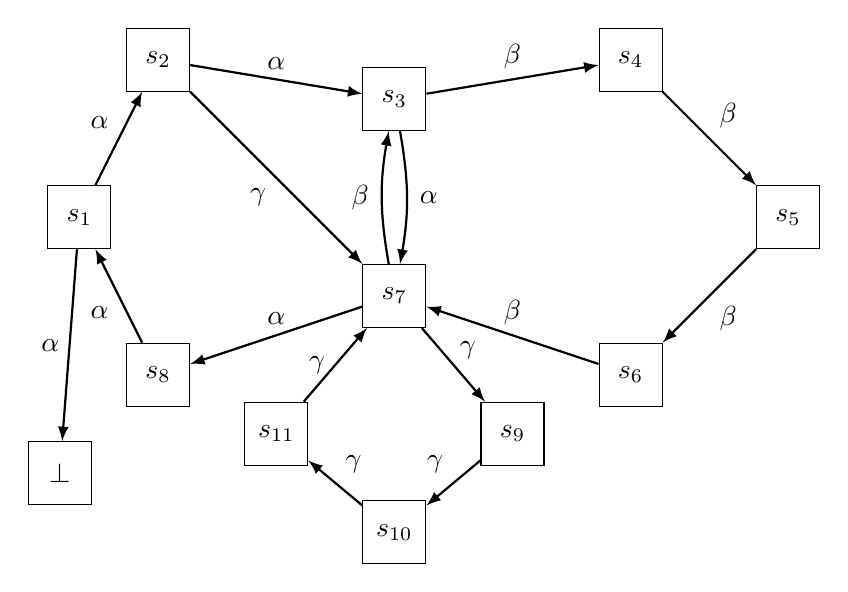
\begin{tikzpicture} 
		%		\createstate{s1}{3,2+4}{$\state_1$};
		\path
		(\basex,		\basey+2) 		node[gstate] (s1) 	{$\state_1$} 
		(\basex+2,		\basey+4) 		node[gstate] (s2) 	{$\state_2$} 
		(\basex+5,		\basey+3.5) 	node[gstate] (s3) 	{$\state_3$} 
		(\basex+8,		\basey+4) 		node[gstate] (s4) 	{$\state_4$}
		(\basex+10,		\basey+2) 		node[gstate] (s5) 	{$\state_5$}
		(\basex+8,		\basey+0) 		node[gstate] (s6) 	{$\state_6$}
		(\basex+5,		\basey+1) 		node[gstate] (s7) 	{$\state_7$}
		(\basex+2,		\basey+0) 		node[gstate] (s8) 	{$\state_8$}
		(\basex+6.5,	\basey-.75)		node[gstate] (s9) 	{$\state_9$}
		(\basex+5,		\basey-2) 		node[gstate] (s10) 	{$\state_{10}$}
		(\basex+3.5,	\basey-.75)		node[gstate] (s11) 	{$\state_{11}$}
		(\basex+.75,	\basey-1.25)	node[gstate] (s12) 	{\notppty}		
		;
		
		\path [trans] (s1) 	edge node [midway,above left]{\action} 		(s2);
		\path [trans] (s2) 	edge node [midway,above]{\action} 			(s3);
		\path [trans] (s3) 	edge node [midway,above]{\actionb} 			(s4);
		\path [trans] (s4) 	edge node [midway,above right]{\actionb} 	(s5);
		\path [trans] (s5)	edge node [midway,below right]{\actionb} 	(s6);
		\path [trans] (s6) 	edge node [midway,above]{\actionb} 			(s7);
		\path [trans] (s7)	edge node [midway,above]{\action} 			(s8);
		\path [trans] (s8) 	edge node [midway,below left]{\action} 			(s1);
		\path [trans] (s7) 	edge node [midway,above right=-2pt]{\actionc} 	(s9);
		\path [trans] (s9) 	edge node [midway,above left]{\actionc} 	(s10);
		\path [trans] (s10)	edge node [midway,above right]{\actionc} 	(s11);
		\path [trans] (s11)	edge node [midway,left]{\actionc} 			(s7);
		\path [trans] (s1)	edge node [midway,left]{\action} 			(s12);
		\path [trans] (s2)	edge node [midway,below left]{\actionc} 	(s7);
		
		\path [bendtrans] (s3) edge node [midway,left=10pt]{\actionb} (s7);
		\path [bendtrans] (s7) edge node [midway,right=10pt]{\action} (s3);
		
		%		\path [trans] (s-1) -- (s-2) node [midway, above] () {\action}
		
		%		(\basex+3,	\basey+1) node[state] (s-bot) {$\bot$}
		%		(s-1)++(-1.2,0) node (s-1-in) {}
		%		(s-3)++(-1.2,0) node (s-3-in) {};
		
		
		%		midway, at start, near start, very near start, at end, near end, very near end
		
		%		\path [trans] (s-1) -- (s-bot);
		%		\path [trans] (s-3) -- (s-bot);
		%		\path [trans] (s-1-in) -- (s-1);
		%		\path [trans] (s-3-in) -- (s-3);
		
		
	\end{tikzpicture}
\end{document}
	\caption{Simplified representation of the \viewN \viewhascycle on \mdp from Figure \ref{fig:cyclesBefore}}
	\label{fig:cycleAfterHas}  
\end{figure}

\begin{figure}[h]
	\begin{minipage}{.5\textwidth}
%		\hspace{5mm}
		\documentclass[tikz,preview]{standalone}
%\usepackage{prelude}

%%%%%%%%%%%%%%%%%%%%%%%%%%%%%%%%%%%% PACKAGES %%%%%%%%%%%%%%%%%%%%%%%%%%%%%%%%%%%%%%%%%%

\usepackage{inputenc,fontenc}
\usepackage[a4paper,margin=3cm]{geometry}
\usepackage[english]{babel}
%\usepackage[german]{babel}
%\usepackage[fixlanguage]{babelbib}


\usepackage{bbold}
\usepackage{amsthm}
\usepackage{amsmath}
\usepackage{amssymb} % doteqdot
\usepackage[dvipsnames]{xcolor}
\usepackage{standalone}
\usepackage{tikz}[mode=buildnew]
\usepackage{cite}
\usepackage{xspace}
\usepackage{relsize}
\usepackage{mathtools} % mathclap
%\usepackage{MnSymbol}
\usepackage{hyperref}
\usepackage{url}
\usepackage{listings} % for code
\usepackage[T1]{fontenc} %<
\hypersetup{
	colorlinks,
	citecolor=black,
	filecolor=black,
	linkcolor=black,
	urlcolor=black
}
\usepackage{pgfplots}
\pgfplotsset{compat=1.18}
%\usepackage{courier} %% Sets font for listing as Courier. But also for url and texttt!
\usepackage{listings, xcolor}
\usepackage{graphicx}
\usepackage{subcaption}

\usetikzlibrary{calc}
%\usepackage{xparse} % \newDocumentCommand for multiple optional arguments
%\usepackage{titlecaps}



%%%%%%%%%%%%%%%%%%%%%%%%%%%%%%%%%%%% THEOREMSTYLES %%%%%%%%%%%%%%%%%%%%%%%%%%%%%%%%%%

\theoremstyle{definition}
\newtheorem{definition}{Definition}[section]
\newtheorem{exmp}{Beispiel}[section]
%\AfterEndEnvironment{definition}{\noindent\ignorespaces}

\theoremstyle{theorem}
\newtheorem{theorem}{Satz}[section]
\newtheorem{proposition}{Proposition}[section]
%\AfterEndEnvironment{theorem}{\noindent\ignorespaces}

\theoremstyle{korollary}
\newtheorem{korollary}{Korollar}[section]
%\AfterEndEnvironment{korollary}{\noindent\ignorespaces}


\tikzset{
	mstate/.style={draw, circle, minimum size=.94cm}, 
	gstate/.style={draw, rectangle, minimum size=.8cm},
	varstate/.style={draw,rectangle, rounded corners, minimum size=1}, 
	trans/.style={draw, ->, thick},
	bendtrans/.style={draw, ->, thick, bend left=10},
	bendtransr/.style={draw, ->, thick, bend right=10},
	init/.style={initial, initial distance=6pt, initial text=},
	every loop/.style={min distance=5pt, looseness=8},
	>=latex
}
\usetikzlibrary{automata,positioning}

%auto shift/.style={auto=right,->,
%	to path={ let \p1=(\tikztostart),\p2=(\tikztotarget),
%		\n1={atan2(\y2-\y1,\x2-\x1)},\n2={\n1+180}
%		in ($(\tikztostart.{\n1})!1mm!270:(\tikztotarget.{\n2})$) -- 
%		($(\tikztotarget.{\n2})!1mm!90:(\tikztostart.{\n1})$) \tikztonodes}},

%%%%%%%%%%%%%%%%%%%%%%%%%%%%%%%%%%% MY MACROS %%%%%%%%%%%%%%%%%%%%%%%%%%%%%%%%%%%%%%%%%
%formatting
\newcommand{\comment}[2]{{\color{#1}#2}}
\newcommand{\redcomment}[1]{{\color{red}#1}}
\newcommand{\purpcomment}[1]{{\color{pink}#1}}
\newcommand{\bluecomment}[1]{{\color{blue}#1}}
\newcommand{\mt}[1]{\ensuremath{{#1}}\xspace}
\newcommand{\mynewcommand}[2]{\newcommand{#1}{\mt{#2}}} %% currently not used becaue of ide highlighting
\newcommand{\arr}{\mt{\to}}

%model checking terms
\newcommand{\mimicrel}{\mt{\mathcal{R}}}
\newcommand{\bisimeq}{\mt{\;\!\sim\;\!}}
\newcommand{\simorder}{\mt{\;\!\preceq\;\!}}
\newcommand{\simequiv}{\mt{\;\!\simeq\;\!}} %command already defined
\newcommand{\relts}{\mt{\;\!\bullet_{_{\tiny{TS}}}\;\!}}
\newcommand{\rel}{\mt{\;\!\bullet\;\!}}

%own names
\newcommand{\nm}[1]{#1\xspace}
\newcommand{\mdpN}{\nm{MDP}}
\newcommand{\mdpsN}{\nm{MDPs}}
\newcommand{\viewN}{\nm{view}}
\newcommand{\viewNC}{\nm{View}}
\newcommand{\viewsN}{\nm{views}}
\newcommand{\viewsNC}{\nm{Views}}
\newcommand{\grpfctsubN}{\nm{detached grouping function}}
\newcommand{\grpfctsubNC}{\nm{detached grouping function}}
\newcommand{\grpfctsubNCC}{\nm{Detached Grouping Function}}
\newcommand{\grpfctN}{\nm{grouping function}}
\newcommand{\grpfctNC}{\nm{Grouping function}}
\newcommand{\grpfctNCC}{\nm{Grouping Function}}
\newcommand{\grpfctsN}{\nm{grouping functions}}
\newcommand{\grpfctsNC}{\nm{Grouping functions}}
\newcommand{\grpfctsNCC}{\nm{Grouping Functions}}
\newcommand{\stmimicN}{\nm{state-mimic}}
\newcommand{\stmimicsN}{\nm{state-mimics}}
\newcommand{\stmimickingN}{\nm{state-mimicking}}
\newcommand{\stmimickedN}{\nm{state-mimicked}}
%\newcommand{\chosenphtypeNCC}{\nm{Transition System}}
%\newcommand{\chgphNC}{\nm{Transition system}}
%\newcommand{\chgphN}{\nm{transition system}}
%\newcommand{\chgphsNCC}{\nm{Transition Systems}}
%\newcommand{\chgphsNC}{\nm{Transition systems}}
%\newcommand{\chgphsN}{\nm{transition systems}}
\newcommand{\chgphNCC}{\nm{MDP}}
\newcommand{\chgphNC}{\nm{MDP}}
\newcommand{\chgphN}{\nm{MDP}}
\newcommand{\achgphN}{\nm{an MDP}}
\newcommand{\chgphsNCC}{\nm{MDPs}}
\newcommand{\chgphsNC}{\nm{MDPs}}
\newcommand{\chgphsN}{\nm{MDPs}}
\newcommand{\parllcompN}{\nm{parallel composition}}
\newcommand{\parllcompNC}{\nm{Parallel composition}}
\newcommand{\parllcompNCC}{\nm{Parallel Composition}}
\newcommand{\parllcompsN}{\nm{parallel compositions}}
\newcommand{\parllcompsNC}{\nm{Parallel compositions}}
\newcommand{\parllcompsNCC}{\nm{Parallel Compositions}}
\newcommand{\sccN}{\nm{SCC}}
\newcommand{\sccsN}{\nm{SCCs}}
\newcommand{\bsccN}{\nm{BSCC}}
\newcommand{\bsccsN}{\nm{BSCCs}}
\newcommand{\jgrapht}{\nm{jGraphtT}}

\newcommand{\outactident}{\nm{OutActionsIdent}}

%names
\newcommand{\iffN}{\nm{if and only if}}
\newcommand{\tsN}{\nm{TS}}

%% outactions identical
\newcommand{\outactidentstrong}{\nm{strong}}
\newcommand{\outactidentweak}{\nm{weak}}

% CORE DEFINITIONS
\newcommand{\grpfct}[1][\viewppty]{\mt{F_{#1}}}
\newcommand{\grpfctsub}[1][\viewppty]{\mt{\tilde{F}_{#1}}}
%\newcommand{\grpfctimg}[1]{\mt{{\grpfct}[{#1}]}}
%\newcommand{\fctimg}[2]{\mt{{#1}[{#2}]}}
\newcommand{\eqrelview}{\mt{R}}
\newcommand{\eqclassv}[1][\state]{\mt{\eqclass{#1}{\eqrelview}}}
\newcommand{\eqclasssetv}[1][\states]{\mt{{#1}/\eqrelview}} %OLD: \bigcup_{\state \in \states} \eqclassv
\newcommand{\viewid}{\mt{\mdp}}
\newcommand{\view}[1][\viewppty]{\mt{\viewid_{#1}}}
\newcommand{\imggrp}{\mt{\arbset}}
\newcommand{\imggrpsub}{\mt{X}}
\newcommand{\viewppty}{\mt{\theta}}
\newcommand{\pll}{\mt{\;\!\pllpure\;\!}}
\newcommand{\pllrev}{\mt{\pllpure^{-1}}}
\newcommand{\pllpure}{\mt{||}}
\newcommand{\compselectset}{\mt{Z}}
\newcommand{\compselectpure}{\mt{\pllpure_\compselectset}}
\newcommand{\compselect}{\mt{\;\pllpure_\compselectset\;}}
\newcommand{\remstates}{\mt{\bigcup_{\state \in \states \setminus \states_1}\{\{\state\}\}}}
\newcommand{\nogroupstates}[1][\states_2]{\mt{\bigcup_{\state \in \states \setminus {#1}}\{\{\state\}\}}}
\newcommand{\remelem}{\mt{\bullet}}
\newcommand{\nogroupset}{\mt{\xi}}
\newcommand{\remset}{\mt{\{\remelem\}}}
\newcommand{\gfctpll}{\mt{\grpfct[\pll]}}
\newcommand{\group}{\mt{\top}}
\newcommand{\imggrpbinview}{\mt{\{\remelem, \notppty\}}}
\newcommand{\viewappset}{\mt{\tilde{\states}}}
\newcommand{\hasppty}{\mt{\top}}
\newcommand{\notppty}{\mt{\bot}}
\newcommand{\disregardelem}{\mt{\Delta}}
\newcommand{\disregardelements}{\mt{{\disregardelem_1, \dots, \disregardelem_n}}}



%\newcommand{\mdp}{def}\mdp
%\newcommand{\mdpdef}



% EXAMPLE VIEWS
\newcommand{\pptyatomicprops}{\mt{\atomicprops}}
\newcommand{\pptyinitstates}{\mt{\initstates}}
\newcommand{\pptyinactsetsize}{\mt{|\inacts(\state)|}}
\newcommand{\pptyhasoutact}{\mt{\exists\outact}}
\newcommand{\pptyminoutact}[2]{\mt{#1\leq#2}}
\newcommand{\pptymaxoutact}[2]{\mt{#2\leq#1}}
\newcommand{\pptyspanoutact}[3]{\mt{#1\leq#2\leq#3}}
\newcommand{\pptyoutactsetsize}{\mt{|\outacts(\state)|}}
\newcommand{\pptyoutactsingle}{\mt{|\outacts(\state)|_1}}
\newcommand{\pptystrongoutactident}{\mt{\outacts(\state)_=}}
\newcommand{\pptyweakoutactident}{\mt{\outacts(\state)_\approx}}
\newcommand{\pptyhasinact}{\mt{\exists\inact}}
\newcommand{\pptymininact}[2]{\mt{#1\leq#2}}
\newcommand{\pptymaxinact}[2]{\mt{#2\leq#1}}
\newcommand{\pptyspaninact}[3]{\mt{#1\leq#2\leq#3}}
\newcommand{\pptyinactsingle}{\mt{|\inacts(\state)|_1}}
\newcommand{\pptystronginactident}{\mt{\inacts(\state)_=}}
\newcommand{\pptyweakinactident}{\mt{\inacts(\state)_\approx}}
\newcommand{\pptyparamvalueseq}{\mt{\var = \varval}}
\newcommand{\pptyparamvaluesneq}{\mt{\var \neq \varval}}
\newcommand{\pptyparamdnf}{\mt{VarDNF}}
\newcommand{\pptyparamcnf}{\mt{VarCNF}}
\newcommand{\pptyparamvalueseqopt}{\mt{\var = \varval}}
\newcommand{\pptyparamvalident}{\mt{Var:\varval}}
\newcommand{\pptydistance}{\mt{\distpath}}
\newcommand{\pptydistancerev}{\mt{\distpathrev}}
\newcommand{\pptydistancebi}{\mt{\distpathbi}}
\newcommand{\pptyhascycle}{\mt{\exists\cycle}}
\newcommand{\pptyexactactcycle}{\mt{\{\cycle_{\action,n}\}}}
\newcommand{\pptycycleset}{\mt{\cup{\{\state\}_\cycle}}}
\newcommand{\pptyexactcycle}{\mt{\{\cycle_n\}}}
\newcommand{\pptyscc}{\mt{scc}}
\newcommand{\pptybscc}{\mt{bscc}}
\newcommand{\pptyprop}{\mt{\redcomment{?}}}
\newcommand{\pptyident}{id}


\newcommand{\gfctatomicprops}{\mt{\grpfct[\pptyatomicprops]}}
\newcommand{\gfctinitstates}{\mt{\grpfct[\pptyinitstates]^\hasppty}}
\newcommand{\gfcthasoutaction}{\mt{\grpfct[\pptyhasoutact]^\hasppty}}
\newcommand{\gfctminoutaction}{\mt{\grpfct[\pptyminoutact{\numoutact}{\outact}]^\hasppty}}
\newcommand{\gfctmaxoutaction}{\mt{\grpfct[\pptymaxoutact{\numoutact}{\outact}]^\hasppty}}
\newcommand{\gfctspanoutaction}{\mt{\grpfct[\pptyspanoutact{\numoutactb}{\outact}{\numoutact}]^\hasppty}}
\newcommand{\gfctoutactsetsize}{\mt{\grpfct[\pptyoutactsetsize]}}
\newcommand{\gfctoutactsingle}{\mt{\grpfct[\pptyoutactsingle]^\notppty}}
\newcommand{\gfctstrongoutactident}{\mt{\grpfct[\pptystrongoutactident]}}
\newcommand{\gfctweakoutactident}{\mt{\grpfct[\pptyweakoutactident]}}
\newcommand{\gfcthasinaction}{\mt{\grpfct[\pptyhasinact]^\hasppty}}
\newcommand{\gfctmininaction}{\mt{\grpfct[\pptymininact{\numinact}{\inact}]^\hasppty}}
\newcommand{\gfctmaxinaction}{\mt{\grpfct[\pptymaxinact{\numinact}{\inact}]^\hasppty}}
\newcommand{\gfctspaninaction}{\mt{\grpfct[\pptyspaninact{\numinactb}{\inact}{\numinact}]^\hasppty}}
\newcommand{\gfctinactsetsize}{\mt{\grpfct[\pptyinactsetsize]}}
\newcommand{\gfctinactsingle}{\mt{\grpfct[\pptyinactsingle]^\notppty}}
\newcommand{\gfctstronginactident}{\mt{\grpfct[\pptystronginactident]}}
\newcommand{\gfctweakinactident}{\mt{\grpfct[\pptyweakinactident]}}
\newcommand{\gfctparamvalueseq}{\mt{\grpfct[\pptyparamvalueseq]^\hasppty}}
\newcommand{\gfctparamvaluesneq}{\mt{\grpfct[\pptyparamvaluesneq]^\hasppty}}
\newcommand{\gfctparamdnf}{\mt{\grpfct[\pptyparamdnf]^\hasppty}}
\newcommand{\gfctparamcnf}{\mt{\grpfct[\pptyparamcnf]^\hasppty}}
\newcommand{\gfctparamvalueseqopt}{\mt{\pptyparamvalueseqopt}}
\newcommand{\gfctparamvalident}{\mt{\grpfct[\pptyparamvalident]}}
\newcommand{\gfctdistance}{\mt{\grpfct[\pptydistance]}}
\newcommand{\gfctdistancerev}{\mt{\grpfct[\pptydistancerev]}}
\newcommand{\gfctdistancebi}{\mt{\grpfct[\pptydistancebi]}}
\newcommand{\gfcthascycle}{\mt{\grpfct[\pptyhascycle]}}
\newcommand{\gfctexactcycle}{\mt{\grpfct[\pptyexactcycle]}}
\newcommand{\gfctcycleset}{\mt{\grpfct[\pptycycleset]}}
\newcommand{\gfctexactactcycle}{\mt{\grpfct[\pptyexactactcycle]}}
\newcommand{\gfctscc}{\mt{\grpfct[\pptyscc]}}
\newcommand{\gfctbscc}{\mt{\grpfct[\pptybscc]}}
\newcommand{\gfctprop}{\mt{\grpfct[\pptyprop]}}
\newcommand{\gfctident}{\mt{\grpfct[\pptyident]}}

\newcommand{\gfctsubatomicprops}{\mt{\grpfctsub[\pptyatomicprops]}}
\newcommand{\gfctsubinitstates}{\mt{\grpfctsub[\pptyinitstates]^\hasppty}}
\newcommand{\gfctsubhasoutaction}{\mt{\grpfctsub[\pptyhasoutact]^\hasppty}}
\newcommand{\gfctsubminoutaction}{\mt{\grpfctsub[\pptyminoutact{\numoutact}{\outact}]^\hasppty}}
\newcommand{\gfctsubmaxoutaction}{\mt{\grpfctsub[\pptymaxoutact{\numoutact}{\outact}]^\hasppty}}
\newcommand{\gfctsubspanoutaction}{\mt{\grpfctsub[\pptyspanoutact{\numoutactb}{\outact}{\numoutact}]^\hasppty}}
\newcommand{\gfctsuboutactsetsize}{\mt{\grpfctsub[\pptyoutactsetsize]}}
\newcommand{\gfctsuboutactsingle}{\mt{\grpfctsub[\pptyoutactsingle]^\notppty}}
\newcommand{\gfctsubstrongoutactident}{\mt{\grpfctsub[\pptystrongoutactident]^\hasppty}}
\newcommand{\gfctsubweakoutactident}{\mt{\grpfctsub[\pptyweakoutactident]^\hasppty}}
\newcommand{\gfctsubhasinaction}{\mt{\grpfctsub[\pptyhasinact]}}
\newcommand{\gfctsubmininaction}{\mt{\grpfctsub[\pptymininact{\numinact}{\inact}]}}
\newcommand{\gfctsubmaxinaction}{\mt{\grpfctsub[\pptymaxinact{\numinact}{\inact}]}}
\newcommand{\gfctsubspaninaction}{\mt{\grpfctsub[\pptyspaninact{\numinactb}{\inact}{\numinact}]}}
\newcommand{\gfctsubinactsetsize}{\mt{\grpfctsub[\pptyinactsetsize]^\hasppty}}
\newcommand{\gfctsubinactsingle}{\mt{\grpfctsub[\pptyinactsingle]^\notppty}}
\newcommand{\gfctsubstronginactident}{\mt{\grpfctsub[\pptystronginactident]}}
\newcommand{\gfctsubweakinactident}{\mt{\grpfctsub[\pptyweakinactident]}}
\newcommand{\gfctsubparamvalueseq}{\mt{\grpfctsub[\pptyparamvalueseq]^\hasppty}}
\newcommand{\gfctsubparamvaluesneq}{\mt{\grpfctsub[\pptyparamvaluesneq]^\hasppty}}
\newcommand{\gfctsubparamdnf}{\mt{\grpfctsub[\pptyparamdnf]^\hasppty}}
\newcommand{\gfctsubparamcnf}{\mt{\grpfctsub[\pptyparamcnf]^\hasppty}}
\newcommand{\gfctsubparamvalueseqopt}{\mt{\pptyparamvalueseqopt}}
\newcommand{\gfctsubparamvalident}{\mt{\grpfctsub[\pptyparamvalident]}}
\newcommand{\gfctsubdistance}{\mt{\grpfctsub[\pptydistance]}}
\newcommand{\gfctsubdistancerev}{\mt{\grpfctsub[\pptydistancerev]}}
\newcommand{\gfctsubdistancebi}{\mt{\grpfctsub[\pptydistancebi]}}
\newcommand{\gfctsubhascycle}{\mt{\grpfctsub[\pptyhascycle]^\hasppty}}
\newcommand{\gfctsubexactcycle}{\mt{\grpfctsub[\pptyexactcycle]}}
\newcommand{\gfctsubcycleset}{\mt{\grpfctsub[\pptycycleset]}}
\newcommand{\gfctsubexactactcycle}{\mt{\grpfctsub[\pptyexactactcycle]}}
\newcommand{\gfctsubscc}{\mt{\grpfctsub[\pptyscc]}}
\newcommand{\gfctsubbscc}{\mt{\grpfctsub[\pptybscc]}}
\newcommand{\gfctsubprop}{\mt{\grpfctsub[\pptyprop]}}
\newcommand{\gfctsubident}{\mt{\grpfctsub[\pptyident]}}


\newcommand{\viewatomicprops}{\mt{\view[\pptyatomicprops]}}
\newcommand{\viewinitstates}{\mt{\view[\pptyinitstates]^\hasppty}}
\newcommand{\viewhasoutaction}{\mt{\view[\pptyhasoutact]^\hasppty}}
\newcommand{\viewminoutaction}{\mt{\view[\pptyminoutact{\numoutact}{\outact}]^\hasppty}}
\newcommand{\viewmaxoutaction}{\mt{\view[\pptymaxoutact{\numoutact}{\outact}]^\hasppty}}
\newcommand{\viewspanoutaction}{\mt{\view[\pptyspanoutact{\numoutactb}{\outact}{\numoutact}]^\hasppty}}
\newcommand{\viewoutactsetsize}{\mt{\view[\pptyoutactsetsize]}}
\newcommand{\viewoutactsingle}{\mt{\view[\pptyoutactsingle]^\notppty}}
\newcommand{\viewstrongoutactident}{\mt{\view[\pptystrongoutactident]}}
\newcommand{\viewweakoutactident}{\mt{\view[\pptyweakoutactident]}}
\newcommand{\viewhasinaction}{\mt{\view[\pptyhasinact]^\hasppty}}
\newcommand{\viewmininaction}{\mt{\view[\pptymininact{\numinact}{\inact}]^\hasppty}}
\newcommand{\viewmaxinaction}{\mt{\view[\pptymaxinact{\numinact}{\inact}]^\hasppty}}
\newcommand{\viewspaninaction}{\mt{\view[\pptyspaninact{\numinactb}{\inact}{\numinact}]^\hasppty}}
\newcommand{\viewinactsetsize}{\mt{\view[\pptyinactsetsize]}}
\newcommand{\viewinactsingle}{\mt{\view[\pptyinactsingle]^\notppty}}
\newcommand{\viewstronginactident}{\mt{\view[\pptystronginactident]}}
\newcommand{\viewweakinactident}{\mt{\view[\pptyweakinactident]}}
\newcommand{\viewparamvalueseq}{\mt{\view[\pptyparamvalueseq]}}
\newcommand{\viewparamvaluesneq}{\mt{\view[\pptyparamvaluesneq]}}
\newcommand{\viewparamdnf}{\mt{\view[\pptyparamdnf]^\hasppty}}
\newcommand{\viewparamcnf}{\mt{\view[\pptyparamcnf]^\hasppty}}
\newcommand{\viewparamvalueseqopt}{\mt{\pptyparamvalueseqopt}}
\newcommand{\viewparamvalident}{\mt{\view[\pptyparamvalident]}}
\newcommand{\viewdistance}{\mt{\view[\pptydistance]}}
\newcommand{\viewdistancerev}{\mt{\view[\pptydistancerev]}}
\newcommand{\viewdistancebi}{\mt{\view[\pptydistancebi]}}
\newcommand{\viewhascycle}{\mt{\view[\pptyhascycle]}}
\newcommand{\viewexactcycle}{\mt{\view[\pptyexactcycle]}}
\newcommand{\viewcycleset}{\mt{\view[\pptycycleset]}}
\newcommand{\viewexactactcycle}{\mt{\view[\pptyexactactcycle]}}
\newcommand{\viewscc}{\mt{\view[\pptyscc]}}
\newcommand{\viewbscc}{\mt{\view[\pptybscc]}}
\newcommand{\viewprop}{\mt{\view[\pptyprop]}}
\newcommand{\viewident}{\mt{\view[\pptyident]}}

%\newcommand{\viewatomicprops}{\mt{\view[\atomicprops]}}
%\newcommand{\viewinitstates}{\mt{\view[\initstates]}}
%\newcommand{\viewhasoutaction}{\mt{\view[\pptyhasoutact]}}
%\newcommand{\viewminoutaction}{\mt{\view[\pptyminoutact{\numoutact}{\outact}]}}
%\newcommand{\viewmaxoutaction}{\mt{\view[\pptymaxoutact{\numoutact}{\outact}]}}
%\newcommand{\viewspanoutaction}{\mt{\view[\pptyspanoutact{\numoutactb}{\outact}{\numoutact}]}}
%\newcommand{\viewoutactsetsize}{\mt{\view[\pptyoutactsetsize]}}
%\newcommand{\viewoutactsingle}{\mt{\view[\pptyoutactsingle]}}
%\newcommand{\viewstrongoutactident}{\mt{\view[\outacts(\state)_=]}}
%\newcommand{\viewweakoutactident}{\mt{\view[\outacts(\state)_\approx]}}
%\newcommand{\viewhasinaction}{\mt{\view[\pptyhasinact]}}
%\newcommand{\viewmininaction}{\mt{\view[\pptymininact{\numinact}{\inact}]}}
%\newcommand{\viewmaxinaction}{\mt{\view[\pptymaxinact{\numinact}{\inact}]}}
%\newcommand{\viewspaninaction}{\mt{\view[\pptyspaninact{\numinactb}{\inact}{\numinact}]}}
%\newcommand{\viewinactsetsize}{\mt{\view[\pptyinactsetsize]}}
%\newcommand{\viewinactsingle}{\mt{\view[\pptyinactsingle]}}
%\newcommand{\viewstronginactident}{\mt{\view[\inacts(\state)_=]}}
%\newcommand{\viewweakinactident}{\mt{\view[\inacts(\state)_\approx]}}
%\newcommand{\viewparamvalueseq}{\mt{\view[\var = \varval]}}
%\newcommand{\viewparamvaluesneq}{\mt{\view[\var \neq \varval]}}
%\newcommand{\viewparamdnf}{\mt{\view[VarDNF]}}
%\newcommand{\viewparamcnf}{\mt{\view[VarCNF]}}
%\newcommand{\viewparamvalident}{\mt{\view[\pptyparamvalident]}}
%\newcommand{\viewdistance}{\mt{\view[\pptydistance]}}
%\newcommand{\viewhascycle}{\mt{\view[\exists\cycle]}}
%\newcommand{\viewexactcycle}{\mt{\view[\pptyexactcycle]}}
%\newcommand{\viewcycleset}{\mt{\view[\pptycycleset]}}
%\newcommand{\viewexactactcycle}{\mt{\view[\pptyexactactcycle]}}
%\newcommand{\viewscc}{\mt{\view[scc]}}
%\newcommand{\viewbscc}{\mt{\view[bscc]}}

%actions
\newcommand{\numoutact}{\mt{n}}
\newcommand{\numoutactb}{\mt{m}}
\newcommand{\numinact}{\mt{n}}
\newcommand{\numinactb}{\mt{m}}

\newcommand{\predmaxoutact}[1][\numoutact]{\mt{Q_{\outact\leq#1}(\state,\state_1, \dots, \state_{#1+1})}}
\newcommand{\predminoutact}[1][\numoutact]{\mt{Q_{#1\leq\outact}(\state,\state_1, \dots, \state_{#1})}}
\newcommand{\formoutact}[1][\state]{\mt{C_{#1,\outact}}}
\newcommand{\predmaxinact}[1][\numinact]{\mt{Q_{\inact\leq#1}(\state,\state_1, \dots, \state_{#1+1})}}
\newcommand{\predmininact}[1][\numinact]{\mt{Q_{#1\leq\inact}(\state,\state_1, \dots, \state_{#1})}}

\newcommand{\outact}[1][\action]{\mt{\overrightarrow{#1}}}
\newcommand{\outacts}{\mt{\overrightarrow{\actions}}}
\newcommand{\inact}{\mt{\overleftarrow{\action}}}
\newcommand{\inacts}[1][\action]{\mt{\overleftarrow{#1}}}

%%Parameters
\newcommand{\vars}[1][\mdp]{\mt{V\!ar_{#1}}}
\newcommand{\var}{\mt{x}}
\newcommand{\varstate}[1][]{\mt{\var_{\state#1}}}
\newcommand{\varval}{\mt{a}}
\newcommand{\vareval}[1][\mdp]{\mt{V\!arEval_{#1}}}
\newcommand{\varevalimg}[1][\mdp]{\mt{\vareval[#1][\states,\vars]}}
\newcommand{\varevalimgset}{\mt{\arbset}}
\newcommand{\someparam}{\mt{\tilde{x}}}
\newcommand{\eqorneq}{\mt{\;\doteqdot\;}}
\newcommand{\varstyle}[2]{\mt{\langle#1,#2\rangle}}




%\makeatletter
%\newcommand{\overleftrightsmallarrow}{\mathpalette{\overarrowsmall@\leftrightarrowfill@}}
%\newcommand{\overrightsmallarrow}{\mathpalette{\overarrowsmall@\rightarrowfill@}}
%\newcommand{\overleftsmallarrow}{\mathpalette{\overarrowsmall@\leftarrowfill@}}
%\newcommand{\overarrowsmall@}[3]{%
%	\vbox{%
%		\ialign{%
%			##\crcr
%			#1{\smaller@style{#2}}\crcr
%			\noalign{\nointerlineskip}%
%			$\m@th\hfil#2#3\hfil$\crcr
%		}%
%	}%
%}
%\def\smaller@style#1{%
%	\ifx#1\displaystyle\scriptstyle\else
%	\ifx#1\textstyle\scriptstyle\else
%	\scriptscriptstyle
%	\fi
%	\fi
%}
%\makeatother
%\newcommand{\te}[1]{\overleftrightsmallarrow{#1}}

% Distance
\newcommand{\fctdist}{\mt{distance}}
\newcommand{\fctdistdefault}{\mt{\fctdist(\chgph, \smstates, \grandist)}}
\newcommand{\distval}{\mt{d}}
\newcommand{\grandist}{\mt{n}}
\let\path\oldpath
\newcommand{\path}{\mt{P}}
\newcommand{\pathbi}{\mt{\bar{\path}}}
\newcommand{\pathsecfull}{\mt{(\state_0, \action_0, \state_1, \action_1, \dots, \action_{n}, \state_{n+1})}}
\newcommand{\lenpath}{\mt{len}}
\newcommand{\pfirst}{\mt{first}}
\newcommand{\plast}{\mt{last}}
\newcommand{\pathset}{\mt{\path_\chgph}}
\newcommand{\pathbiset}{\mt{\pathbi_\chgph}}
\newcommand{\distpath}{\mt{\overrightarrow{dist}}}
\newcommand{\distpathrev}{\mt{\overleftarrow{dist}}}
\newcommand{\distpathbi}{\mt{\overline{dist}}}
%Cycles
\newcommand{\cyclesecfull}{\mt{(\state_0, \action_0, \state_1, \action_1, \dots, \action_{n-1}, \state_0)}}
\newcommand{\fctfindcycles}{\mt{findCycles}}
\newcommand{\cycle}{\mt{C}}
\newcommand{\cycleset}{\mt{\cycle_{\mdp, n}}}
\newcommand{\lencycle}{\mt{len}}
% strongly connected components
\newcommand{\scc}{\mt{T}}
\newcommand{\setscc}{\mt{SCC_{\chgph,n}}}
\newcommand{\setbscc}{\mt{BSCC_{\chgph,n}}}

% properties
\newcommand{\propfct}{\mt{f}}

% all Systems
\newcommand{\chgph}{\mt{\mdp}}
\newcommand{\chgphtuple}{\mt{\mdptuple}}
\newcommand{\chgphtupledist}{\mt{\mdptupledist}}

\newcommand{\states}{\mt{S}}
\newcommand{\actions}{\mt{Act}}
\newcommand{\atomicprops}{\mt{AP}}
\newcommand{\labelingfct}{\mt{L}}
\newcommand{\init}{\mt{\initdistrib}} % use MDP % refers to the underlying set
\newcommand{\trans}{\mt{\probtfunc}} % use MDP % refers to the underlying set
\newcommand{\smstates}{\mt{\tilde{\states}}}


\newcommand{\state}{\mt{s}}
\newcommand{\action}{\mt{\alpha}}
\newcommand{\actionb}{\mt{\beta}}
\newcommand{\actionc}{\mt{\gamma}}
\newcommand{\smstate}{\mt{\tilde{\state}}}



% transition sysstems
\newcommand{\ts}{\mt{TS}}
\newcommand{\transitionrel}{\mt{\longrightarrow}}
\newcommand{\initstates}{\mt{I}}
\newcommand{\transitionsystem}{\mt
	{(\states, \actions, \transitionrel, \initstates, \atomicprops, \labelingfct)}
}
\newcommand{\tstupledist}{\mt{(\states', \actions',\transitionrel', \initstates', \labelingfct')}}


%Markov chains and MDP
\newcommand{\mdp}{\mt{\autm}}
\newcommand{\mdptuple}{\mt{(\states, \actions, \probtfunc, \initdistrib, \atomicprops, \labelingfct)}}
\newcommand{\mdptupledist}{\mt{(\states', \actions', \probtfunc', \initdistrib', \atomicprops', \labelingfct')}}
\newcommand{\autm}{\mt{\mathcal{M}}}
\newcommand{\probtfunc}{\mt{\textbf{P}}}
\newcommand{\initdistrib}{\mt{\iota_{init}}}


%maths
\newcommand{\powerset}[1]{\mt{\mathcal{P}(#1)}}
\newcommand{\eqclass}[2]{\mt{[#1]_{#2}}}%{\mt{#1 / #2}}
\newcommand{\impr}{\mt{\hspace{3mm}\Rightarrow\hspace{2mm}}}
\newcommand{\impl}{\mt{\hspace{3mm}\Leftarrow\hspace{2mm}}}
\newcommand{\natnums}{\mt{\mathbb{N}}} 
\newcommand{\realnums}{\mt{\mathbb{R}}}
\newcommand{\intmodn}[1][n]{\mt{\mathbb{Z}_{#1}}}
\newcommand{\arbset}{\mt{M}}
\newcommand{\bigsum}[2][]{\mt{\mathlarger{\sum}_{#2}^{#1}}}
\newcommand{\bbigsum}[2][]{\mt{\mathlarger{\mathlarger{\sum}}_{#2}^{#1}}}
\newcommand{\invimage}[2]{#1^{\mt{-1}(#2)}}
\newcommand{\img}{\mt{Img}}
\newcommand{\cond}{\mt{\,|\,}}

%tickz
%% \definecolor{darkred}{RGB}{196, 42, 42}

%implementation
\newcommand{\pmcvis}{\nm{PMC-Vis}}


\usepackage{tikz}


\begin{document}
	\newcommand{\createstate}[3]{\node[draw, circle, minimum size=1cm] (#1) at (#2) {#3}}
	\newcommand{\basex}{0}
	\newcommand{\basey}{0}
	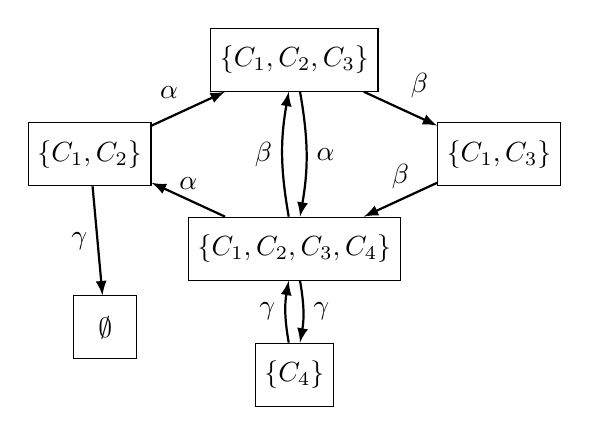
\begin{tikzpicture} [scale=0.8]
		%		\createstate{s1}{3,2+4}{$\state_1$};
		\path
		(\basex+1.75,	\basey+4.5) 	node[gstate] (c12) 		{$\{\cycle_1, \cycle_2\}$} 		
		(\basex+8.25,	\basey+4.5) 	node[gstate] (c13) 		{$\{\cycle_1, \cycle_3\}$}
		(\basex+5,		\basey+1) 	node[gstate] (c4) 		{$\{\cycle_4\}$}
		(\basex+5,		\basey+6) 	node[gstate] (c123) 		{$\{\cycle_1, \cycle_2, \cycle_3\}$} 
		(\basex+5,		\basey+3) 	node[gstate] (c1234) 	{$\{\cycle_1, \cycle_2, \cycle_3, \cycle_4\}$} 
		(\basex+2,		\basey+1.75) 	node[gstate] (cmpty) 	{$\emptyset$} 
		
		;
		
		\path [trans] (c12) edge node [midway, above left] {\action} (c123);
		\path [trans] (c123) edge node [midway, above right] {\actionb} (c13);
		\path [trans] (c13) edge node [midway, above] {\actionb} (c1234);
		\path [bendtrans] (c4) edge node [midway, left] {\actionc} (c1234);
		\path [bendtrans] (c1234) edge node [midway, right] {\actionc} (c4);
		\path [bendtrans] (c1234) edge node [midway, left] {\actionb} (c123);
		\path [bendtrans] (c123) edge node [midway, right] {\action} (c1234);
		\path [trans] (c1234) edge node [midway, above] {\action} (c12);
		\path [trans] (c12) edge node [midway,left] {\actionc} (cmpty);		
		
	\end{tikzpicture}
\end{document}
	\end{minipage}%
	\begin{minipage}{.5\textwidth}
		\documentclass[tikz,preview]{standalone}
%\usepackage{prelude}

%%%%%%%%%%%%%%%%%%%%%%%%%%%%%%%%%%%% PACKAGES %%%%%%%%%%%%%%%%%%%%%%%%%%%%%%%%%%%%%%%%%%

\usepackage{inputenc,fontenc}
\usepackage[a4paper,margin=3cm]{geometry}
\usepackage[english]{babel}
%\usepackage[german]{babel}
%\usepackage[fixlanguage]{babelbib}


\usepackage{bbold}
\usepackage{amsthm}
\usepackage{amsmath}
\usepackage{amssymb} % doteqdot
\usepackage[dvipsnames]{xcolor}
\usepackage{standalone}
\usepackage{tikz}[mode=buildnew]
\usepackage{cite}
\usepackage{xspace}
\usepackage{relsize}
\usepackage{mathtools} % mathclap
%\usepackage{MnSymbol}
\usepackage{hyperref}
\usepackage{url}
\usepackage{listings} % for code
\usepackage[T1]{fontenc} %<
\hypersetup{
	colorlinks,
	citecolor=black,
	filecolor=black,
	linkcolor=black,
	urlcolor=black
}
\usepackage{pgfplots}
\pgfplotsset{compat=1.18}
%\usepackage{courier} %% Sets font for listing as Courier. But also for url and texttt!
\usepackage{listings, xcolor}
\usepackage{graphicx}
\usepackage{subcaption}

\usetikzlibrary{calc}
%\usepackage{xparse} % \newDocumentCommand for multiple optional arguments
%\usepackage{titlecaps}



%%%%%%%%%%%%%%%%%%%%%%%%%%%%%%%%%%%% THEOREMSTYLES %%%%%%%%%%%%%%%%%%%%%%%%%%%%%%%%%%

\theoremstyle{definition}
\newtheorem{definition}{Definition}[section]
\newtheorem{exmp}{Beispiel}[section]
%\AfterEndEnvironment{definition}{\noindent\ignorespaces}

\theoremstyle{theorem}
\newtheorem{theorem}{Satz}[section]
\newtheorem{proposition}{Proposition}[section]
%\AfterEndEnvironment{theorem}{\noindent\ignorespaces}

\theoremstyle{korollary}
\newtheorem{korollary}{Korollar}[section]
%\AfterEndEnvironment{korollary}{\noindent\ignorespaces}


\tikzset{
	mstate/.style={draw, circle, minimum size=.94cm}, 
	gstate/.style={draw, rectangle, minimum size=.8cm},
	varstate/.style={draw,rectangle, rounded corners, minimum size=1}, 
	trans/.style={draw, ->, thick},
	bendtrans/.style={draw, ->, thick, bend left=10},
	bendtransr/.style={draw, ->, thick, bend right=10},
	init/.style={initial, initial distance=6pt, initial text=},
	every loop/.style={min distance=5pt, looseness=8},
	>=latex
}
\usetikzlibrary{automata,positioning}

%auto shift/.style={auto=right,->,
%	to path={ let \p1=(\tikztostart),\p2=(\tikztotarget),
%		\n1={atan2(\y2-\y1,\x2-\x1)},\n2={\n1+180}
%		in ($(\tikztostart.{\n1})!1mm!270:(\tikztotarget.{\n2})$) -- 
%		($(\tikztotarget.{\n2})!1mm!90:(\tikztostart.{\n1})$) \tikztonodes}},

%%%%%%%%%%%%%%%%%%%%%%%%%%%%%%%%%%% MY MACROS %%%%%%%%%%%%%%%%%%%%%%%%%%%%%%%%%%%%%%%%%
%formatting
\newcommand{\comment}[2]{{\color{#1}#2}}
\newcommand{\redcomment}[1]{{\color{red}#1}}
\newcommand{\purpcomment}[1]{{\color{pink}#1}}
\newcommand{\bluecomment}[1]{{\color{blue}#1}}
\newcommand{\mt}[1]{\ensuremath{{#1}}\xspace}
\newcommand{\mynewcommand}[2]{\newcommand{#1}{\mt{#2}}} %% currently not used becaue of ide highlighting
\newcommand{\arr}{\mt{\to}}

%model checking terms
\newcommand{\mimicrel}{\mt{\mathcal{R}}}
\newcommand{\bisimeq}{\mt{\;\!\sim\;\!}}
\newcommand{\simorder}{\mt{\;\!\preceq\;\!}}
\newcommand{\simequiv}{\mt{\;\!\simeq\;\!}} %command already defined
\newcommand{\relts}{\mt{\;\!\bullet_{_{\tiny{TS}}}\;\!}}
\newcommand{\rel}{\mt{\;\!\bullet\;\!}}

%own names
\newcommand{\nm}[1]{#1\xspace}
\newcommand{\mdpN}{\nm{MDP}}
\newcommand{\mdpsN}{\nm{MDPs}}
\newcommand{\viewN}{\nm{view}}
\newcommand{\viewNC}{\nm{View}}
\newcommand{\viewsN}{\nm{views}}
\newcommand{\viewsNC}{\nm{Views}}
\newcommand{\grpfctsubN}{\nm{detached grouping function}}
\newcommand{\grpfctsubNC}{\nm{detached grouping function}}
\newcommand{\grpfctsubNCC}{\nm{Detached Grouping Function}}
\newcommand{\grpfctN}{\nm{grouping function}}
\newcommand{\grpfctNC}{\nm{Grouping function}}
\newcommand{\grpfctNCC}{\nm{Grouping Function}}
\newcommand{\grpfctsN}{\nm{grouping functions}}
\newcommand{\grpfctsNC}{\nm{Grouping functions}}
\newcommand{\grpfctsNCC}{\nm{Grouping Functions}}
\newcommand{\stmimicN}{\nm{state-mimic}}
\newcommand{\stmimicsN}{\nm{state-mimics}}
\newcommand{\stmimickingN}{\nm{state-mimicking}}
\newcommand{\stmimickedN}{\nm{state-mimicked}}
%\newcommand{\chosenphtypeNCC}{\nm{Transition System}}
%\newcommand{\chgphNC}{\nm{Transition system}}
%\newcommand{\chgphN}{\nm{transition system}}
%\newcommand{\chgphsNCC}{\nm{Transition Systems}}
%\newcommand{\chgphsNC}{\nm{Transition systems}}
%\newcommand{\chgphsN}{\nm{transition systems}}
\newcommand{\chgphNCC}{\nm{MDP}}
\newcommand{\chgphNC}{\nm{MDP}}
\newcommand{\chgphN}{\nm{MDP}}
\newcommand{\achgphN}{\nm{an MDP}}
\newcommand{\chgphsNCC}{\nm{MDPs}}
\newcommand{\chgphsNC}{\nm{MDPs}}
\newcommand{\chgphsN}{\nm{MDPs}}
\newcommand{\parllcompN}{\nm{parallel composition}}
\newcommand{\parllcompNC}{\nm{Parallel composition}}
\newcommand{\parllcompNCC}{\nm{Parallel Composition}}
\newcommand{\parllcompsN}{\nm{parallel compositions}}
\newcommand{\parllcompsNC}{\nm{Parallel compositions}}
\newcommand{\parllcompsNCC}{\nm{Parallel Compositions}}
\newcommand{\sccN}{\nm{SCC}}
\newcommand{\sccsN}{\nm{SCCs}}
\newcommand{\bsccN}{\nm{BSCC}}
\newcommand{\bsccsN}{\nm{BSCCs}}
\newcommand{\jgrapht}{\nm{jGraphtT}}

\newcommand{\outactident}{\nm{OutActionsIdent}}

%names
\newcommand{\iffN}{\nm{if and only if}}
\newcommand{\tsN}{\nm{TS}}

%% outactions identical
\newcommand{\outactidentstrong}{\nm{strong}}
\newcommand{\outactidentweak}{\nm{weak}}

% CORE DEFINITIONS
\newcommand{\grpfct}[1][\viewppty]{\mt{F_{#1}}}
\newcommand{\grpfctsub}[1][\viewppty]{\mt{\tilde{F}_{#1}}}
%\newcommand{\grpfctimg}[1]{\mt{{\grpfct}[{#1}]}}
%\newcommand{\fctimg}[2]{\mt{{#1}[{#2}]}}
\newcommand{\eqrelview}{\mt{R}}
\newcommand{\eqclassv}[1][\state]{\mt{\eqclass{#1}{\eqrelview}}}
\newcommand{\eqclasssetv}[1][\states]{\mt{{#1}/\eqrelview}} %OLD: \bigcup_{\state \in \states} \eqclassv
\newcommand{\viewid}{\mt{\mdp}}
\newcommand{\view}[1][\viewppty]{\mt{\viewid_{#1}}}
\newcommand{\imggrp}{\mt{\arbset}}
\newcommand{\imggrpsub}{\mt{X}}
\newcommand{\viewppty}{\mt{\theta}}
\newcommand{\pll}{\mt{\;\!\pllpure\;\!}}
\newcommand{\pllrev}{\mt{\pllpure^{-1}}}
\newcommand{\pllpure}{\mt{||}}
\newcommand{\compselectset}{\mt{Z}}
\newcommand{\compselectpure}{\mt{\pllpure_\compselectset}}
\newcommand{\compselect}{\mt{\;\pllpure_\compselectset\;}}
\newcommand{\remstates}{\mt{\bigcup_{\state \in \states \setminus \states_1}\{\{\state\}\}}}
\newcommand{\nogroupstates}[1][\states_2]{\mt{\bigcup_{\state \in \states \setminus {#1}}\{\{\state\}\}}}
\newcommand{\remelem}{\mt{\bullet}}
\newcommand{\nogroupset}{\mt{\xi}}
\newcommand{\remset}{\mt{\{\remelem\}}}
\newcommand{\gfctpll}{\mt{\grpfct[\pll]}}
\newcommand{\group}{\mt{\top}}
\newcommand{\imggrpbinview}{\mt{\{\remelem, \notppty\}}}
\newcommand{\viewappset}{\mt{\tilde{\states}}}
\newcommand{\hasppty}{\mt{\top}}
\newcommand{\notppty}{\mt{\bot}}
\newcommand{\disregardelem}{\mt{\Delta}}
\newcommand{\disregardelements}{\mt{{\disregardelem_1, \dots, \disregardelem_n}}}



%\newcommand{\mdp}{def}\mdp
%\newcommand{\mdpdef}



% EXAMPLE VIEWS
\newcommand{\pptyatomicprops}{\mt{\atomicprops}}
\newcommand{\pptyinitstates}{\mt{\initstates}}
\newcommand{\pptyinactsetsize}{\mt{|\inacts(\state)|}}
\newcommand{\pptyhasoutact}{\mt{\exists\outact}}
\newcommand{\pptyminoutact}[2]{\mt{#1\leq#2}}
\newcommand{\pptymaxoutact}[2]{\mt{#2\leq#1}}
\newcommand{\pptyspanoutact}[3]{\mt{#1\leq#2\leq#3}}
\newcommand{\pptyoutactsetsize}{\mt{|\outacts(\state)|}}
\newcommand{\pptyoutactsingle}{\mt{|\outacts(\state)|_1}}
\newcommand{\pptystrongoutactident}{\mt{\outacts(\state)_=}}
\newcommand{\pptyweakoutactident}{\mt{\outacts(\state)_\approx}}
\newcommand{\pptyhasinact}{\mt{\exists\inact}}
\newcommand{\pptymininact}[2]{\mt{#1\leq#2}}
\newcommand{\pptymaxinact}[2]{\mt{#2\leq#1}}
\newcommand{\pptyspaninact}[3]{\mt{#1\leq#2\leq#3}}
\newcommand{\pptyinactsingle}{\mt{|\inacts(\state)|_1}}
\newcommand{\pptystronginactident}{\mt{\inacts(\state)_=}}
\newcommand{\pptyweakinactident}{\mt{\inacts(\state)_\approx}}
\newcommand{\pptyparamvalueseq}{\mt{\var = \varval}}
\newcommand{\pptyparamvaluesneq}{\mt{\var \neq \varval}}
\newcommand{\pptyparamdnf}{\mt{VarDNF}}
\newcommand{\pptyparamcnf}{\mt{VarCNF}}
\newcommand{\pptyparamvalueseqopt}{\mt{\var = \varval}}
\newcommand{\pptyparamvalident}{\mt{Var:\varval}}
\newcommand{\pptydistance}{\mt{\distpath}}
\newcommand{\pptydistancerev}{\mt{\distpathrev}}
\newcommand{\pptydistancebi}{\mt{\distpathbi}}
\newcommand{\pptyhascycle}{\mt{\exists\cycle}}
\newcommand{\pptyexactactcycle}{\mt{\{\cycle_{\action,n}\}}}
\newcommand{\pptycycleset}{\mt{\cup{\{\state\}_\cycle}}}
\newcommand{\pptyexactcycle}{\mt{\{\cycle_n\}}}
\newcommand{\pptyscc}{\mt{scc}}
\newcommand{\pptybscc}{\mt{bscc}}
\newcommand{\pptyprop}{\mt{\redcomment{?}}}
\newcommand{\pptyident}{id}


\newcommand{\gfctatomicprops}{\mt{\grpfct[\pptyatomicprops]}}
\newcommand{\gfctinitstates}{\mt{\grpfct[\pptyinitstates]^\hasppty}}
\newcommand{\gfcthasoutaction}{\mt{\grpfct[\pptyhasoutact]^\hasppty}}
\newcommand{\gfctminoutaction}{\mt{\grpfct[\pptyminoutact{\numoutact}{\outact}]^\hasppty}}
\newcommand{\gfctmaxoutaction}{\mt{\grpfct[\pptymaxoutact{\numoutact}{\outact}]^\hasppty}}
\newcommand{\gfctspanoutaction}{\mt{\grpfct[\pptyspanoutact{\numoutactb}{\outact}{\numoutact}]^\hasppty}}
\newcommand{\gfctoutactsetsize}{\mt{\grpfct[\pptyoutactsetsize]}}
\newcommand{\gfctoutactsingle}{\mt{\grpfct[\pptyoutactsingle]^\notppty}}
\newcommand{\gfctstrongoutactident}{\mt{\grpfct[\pptystrongoutactident]}}
\newcommand{\gfctweakoutactident}{\mt{\grpfct[\pptyweakoutactident]}}
\newcommand{\gfcthasinaction}{\mt{\grpfct[\pptyhasinact]^\hasppty}}
\newcommand{\gfctmininaction}{\mt{\grpfct[\pptymininact{\numinact}{\inact}]^\hasppty}}
\newcommand{\gfctmaxinaction}{\mt{\grpfct[\pptymaxinact{\numinact}{\inact}]^\hasppty}}
\newcommand{\gfctspaninaction}{\mt{\grpfct[\pptyspaninact{\numinactb}{\inact}{\numinact}]^\hasppty}}
\newcommand{\gfctinactsetsize}{\mt{\grpfct[\pptyinactsetsize]}}
\newcommand{\gfctinactsingle}{\mt{\grpfct[\pptyinactsingle]^\notppty}}
\newcommand{\gfctstronginactident}{\mt{\grpfct[\pptystronginactident]}}
\newcommand{\gfctweakinactident}{\mt{\grpfct[\pptyweakinactident]}}
\newcommand{\gfctparamvalueseq}{\mt{\grpfct[\pptyparamvalueseq]^\hasppty}}
\newcommand{\gfctparamvaluesneq}{\mt{\grpfct[\pptyparamvaluesneq]^\hasppty}}
\newcommand{\gfctparamdnf}{\mt{\grpfct[\pptyparamdnf]^\hasppty}}
\newcommand{\gfctparamcnf}{\mt{\grpfct[\pptyparamcnf]^\hasppty}}
\newcommand{\gfctparamvalueseqopt}{\mt{\pptyparamvalueseqopt}}
\newcommand{\gfctparamvalident}{\mt{\grpfct[\pptyparamvalident]}}
\newcommand{\gfctdistance}{\mt{\grpfct[\pptydistance]}}
\newcommand{\gfctdistancerev}{\mt{\grpfct[\pptydistancerev]}}
\newcommand{\gfctdistancebi}{\mt{\grpfct[\pptydistancebi]}}
\newcommand{\gfcthascycle}{\mt{\grpfct[\pptyhascycle]}}
\newcommand{\gfctexactcycle}{\mt{\grpfct[\pptyexactcycle]}}
\newcommand{\gfctcycleset}{\mt{\grpfct[\pptycycleset]}}
\newcommand{\gfctexactactcycle}{\mt{\grpfct[\pptyexactactcycle]}}
\newcommand{\gfctscc}{\mt{\grpfct[\pptyscc]}}
\newcommand{\gfctbscc}{\mt{\grpfct[\pptybscc]}}
\newcommand{\gfctprop}{\mt{\grpfct[\pptyprop]}}
\newcommand{\gfctident}{\mt{\grpfct[\pptyident]}}

\newcommand{\gfctsubatomicprops}{\mt{\grpfctsub[\pptyatomicprops]}}
\newcommand{\gfctsubinitstates}{\mt{\grpfctsub[\pptyinitstates]^\hasppty}}
\newcommand{\gfctsubhasoutaction}{\mt{\grpfctsub[\pptyhasoutact]^\hasppty}}
\newcommand{\gfctsubminoutaction}{\mt{\grpfctsub[\pptyminoutact{\numoutact}{\outact}]^\hasppty}}
\newcommand{\gfctsubmaxoutaction}{\mt{\grpfctsub[\pptymaxoutact{\numoutact}{\outact}]^\hasppty}}
\newcommand{\gfctsubspanoutaction}{\mt{\grpfctsub[\pptyspanoutact{\numoutactb}{\outact}{\numoutact}]^\hasppty}}
\newcommand{\gfctsuboutactsetsize}{\mt{\grpfctsub[\pptyoutactsetsize]}}
\newcommand{\gfctsuboutactsingle}{\mt{\grpfctsub[\pptyoutactsingle]^\notppty}}
\newcommand{\gfctsubstrongoutactident}{\mt{\grpfctsub[\pptystrongoutactident]^\hasppty}}
\newcommand{\gfctsubweakoutactident}{\mt{\grpfctsub[\pptyweakoutactident]^\hasppty}}
\newcommand{\gfctsubhasinaction}{\mt{\grpfctsub[\pptyhasinact]}}
\newcommand{\gfctsubmininaction}{\mt{\grpfctsub[\pptymininact{\numinact}{\inact}]}}
\newcommand{\gfctsubmaxinaction}{\mt{\grpfctsub[\pptymaxinact{\numinact}{\inact}]}}
\newcommand{\gfctsubspaninaction}{\mt{\grpfctsub[\pptyspaninact{\numinactb}{\inact}{\numinact}]}}
\newcommand{\gfctsubinactsetsize}{\mt{\grpfctsub[\pptyinactsetsize]^\hasppty}}
\newcommand{\gfctsubinactsingle}{\mt{\grpfctsub[\pptyinactsingle]^\notppty}}
\newcommand{\gfctsubstronginactident}{\mt{\grpfctsub[\pptystronginactident]}}
\newcommand{\gfctsubweakinactident}{\mt{\grpfctsub[\pptyweakinactident]}}
\newcommand{\gfctsubparamvalueseq}{\mt{\grpfctsub[\pptyparamvalueseq]^\hasppty}}
\newcommand{\gfctsubparamvaluesneq}{\mt{\grpfctsub[\pptyparamvaluesneq]^\hasppty}}
\newcommand{\gfctsubparamdnf}{\mt{\grpfctsub[\pptyparamdnf]^\hasppty}}
\newcommand{\gfctsubparamcnf}{\mt{\grpfctsub[\pptyparamcnf]^\hasppty}}
\newcommand{\gfctsubparamvalueseqopt}{\mt{\pptyparamvalueseqopt}}
\newcommand{\gfctsubparamvalident}{\mt{\grpfctsub[\pptyparamvalident]}}
\newcommand{\gfctsubdistance}{\mt{\grpfctsub[\pptydistance]}}
\newcommand{\gfctsubdistancerev}{\mt{\grpfctsub[\pptydistancerev]}}
\newcommand{\gfctsubdistancebi}{\mt{\grpfctsub[\pptydistancebi]}}
\newcommand{\gfctsubhascycle}{\mt{\grpfctsub[\pptyhascycle]^\hasppty}}
\newcommand{\gfctsubexactcycle}{\mt{\grpfctsub[\pptyexactcycle]}}
\newcommand{\gfctsubcycleset}{\mt{\grpfctsub[\pptycycleset]}}
\newcommand{\gfctsubexactactcycle}{\mt{\grpfctsub[\pptyexactactcycle]}}
\newcommand{\gfctsubscc}{\mt{\grpfctsub[\pptyscc]}}
\newcommand{\gfctsubbscc}{\mt{\grpfctsub[\pptybscc]}}
\newcommand{\gfctsubprop}{\mt{\grpfctsub[\pptyprop]}}
\newcommand{\gfctsubident}{\mt{\grpfctsub[\pptyident]}}


\newcommand{\viewatomicprops}{\mt{\view[\pptyatomicprops]}}
\newcommand{\viewinitstates}{\mt{\view[\pptyinitstates]^\hasppty}}
\newcommand{\viewhasoutaction}{\mt{\view[\pptyhasoutact]^\hasppty}}
\newcommand{\viewminoutaction}{\mt{\view[\pptyminoutact{\numoutact}{\outact}]^\hasppty}}
\newcommand{\viewmaxoutaction}{\mt{\view[\pptymaxoutact{\numoutact}{\outact}]^\hasppty}}
\newcommand{\viewspanoutaction}{\mt{\view[\pptyspanoutact{\numoutactb}{\outact}{\numoutact}]^\hasppty}}
\newcommand{\viewoutactsetsize}{\mt{\view[\pptyoutactsetsize]}}
\newcommand{\viewoutactsingle}{\mt{\view[\pptyoutactsingle]^\notppty}}
\newcommand{\viewstrongoutactident}{\mt{\view[\pptystrongoutactident]}}
\newcommand{\viewweakoutactident}{\mt{\view[\pptyweakoutactident]}}
\newcommand{\viewhasinaction}{\mt{\view[\pptyhasinact]^\hasppty}}
\newcommand{\viewmininaction}{\mt{\view[\pptymininact{\numinact}{\inact}]^\hasppty}}
\newcommand{\viewmaxinaction}{\mt{\view[\pptymaxinact{\numinact}{\inact}]^\hasppty}}
\newcommand{\viewspaninaction}{\mt{\view[\pptyspaninact{\numinactb}{\inact}{\numinact}]^\hasppty}}
\newcommand{\viewinactsetsize}{\mt{\view[\pptyinactsetsize]}}
\newcommand{\viewinactsingle}{\mt{\view[\pptyinactsingle]^\notppty}}
\newcommand{\viewstronginactident}{\mt{\view[\pptystronginactident]}}
\newcommand{\viewweakinactident}{\mt{\view[\pptyweakinactident]}}
\newcommand{\viewparamvalueseq}{\mt{\view[\pptyparamvalueseq]}}
\newcommand{\viewparamvaluesneq}{\mt{\view[\pptyparamvaluesneq]}}
\newcommand{\viewparamdnf}{\mt{\view[\pptyparamdnf]^\hasppty}}
\newcommand{\viewparamcnf}{\mt{\view[\pptyparamcnf]^\hasppty}}
\newcommand{\viewparamvalueseqopt}{\mt{\pptyparamvalueseqopt}}
\newcommand{\viewparamvalident}{\mt{\view[\pptyparamvalident]}}
\newcommand{\viewdistance}{\mt{\view[\pptydistance]}}
\newcommand{\viewdistancerev}{\mt{\view[\pptydistancerev]}}
\newcommand{\viewdistancebi}{\mt{\view[\pptydistancebi]}}
\newcommand{\viewhascycle}{\mt{\view[\pptyhascycle]}}
\newcommand{\viewexactcycle}{\mt{\view[\pptyexactcycle]}}
\newcommand{\viewcycleset}{\mt{\view[\pptycycleset]}}
\newcommand{\viewexactactcycle}{\mt{\view[\pptyexactactcycle]}}
\newcommand{\viewscc}{\mt{\view[\pptyscc]}}
\newcommand{\viewbscc}{\mt{\view[\pptybscc]}}
\newcommand{\viewprop}{\mt{\view[\pptyprop]}}
\newcommand{\viewident}{\mt{\view[\pptyident]}}

%\newcommand{\viewatomicprops}{\mt{\view[\atomicprops]}}
%\newcommand{\viewinitstates}{\mt{\view[\initstates]}}
%\newcommand{\viewhasoutaction}{\mt{\view[\pptyhasoutact]}}
%\newcommand{\viewminoutaction}{\mt{\view[\pptyminoutact{\numoutact}{\outact}]}}
%\newcommand{\viewmaxoutaction}{\mt{\view[\pptymaxoutact{\numoutact}{\outact}]}}
%\newcommand{\viewspanoutaction}{\mt{\view[\pptyspanoutact{\numoutactb}{\outact}{\numoutact}]}}
%\newcommand{\viewoutactsetsize}{\mt{\view[\pptyoutactsetsize]}}
%\newcommand{\viewoutactsingle}{\mt{\view[\pptyoutactsingle]}}
%\newcommand{\viewstrongoutactident}{\mt{\view[\outacts(\state)_=]}}
%\newcommand{\viewweakoutactident}{\mt{\view[\outacts(\state)_\approx]}}
%\newcommand{\viewhasinaction}{\mt{\view[\pptyhasinact]}}
%\newcommand{\viewmininaction}{\mt{\view[\pptymininact{\numinact}{\inact}]}}
%\newcommand{\viewmaxinaction}{\mt{\view[\pptymaxinact{\numinact}{\inact}]}}
%\newcommand{\viewspaninaction}{\mt{\view[\pptyspaninact{\numinactb}{\inact}{\numinact}]}}
%\newcommand{\viewinactsetsize}{\mt{\view[\pptyinactsetsize]}}
%\newcommand{\viewinactsingle}{\mt{\view[\pptyinactsingle]}}
%\newcommand{\viewstronginactident}{\mt{\view[\inacts(\state)_=]}}
%\newcommand{\viewweakinactident}{\mt{\view[\inacts(\state)_\approx]}}
%\newcommand{\viewparamvalueseq}{\mt{\view[\var = \varval]}}
%\newcommand{\viewparamvaluesneq}{\mt{\view[\var \neq \varval]}}
%\newcommand{\viewparamdnf}{\mt{\view[VarDNF]}}
%\newcommand{\viewparamcnf}{\mt{\view[VarCNF]}}
%\newcommand{\viewparamvalident}{\mt{\view[\pptyparamvalident]}}
%\newcommand{\viewdistance}{\mt{\view[\pptydistance]}}
%\newcommand{\viewhascycle}{\mt{\view[\exists\cycle]}}
%\newcommand{\viewexactcycle}{\mt{\view[\pptyexactcycle]}}
%\newcommand{\viewcycleset}{\mt{\view[\pptycycleset]}}
%\newcommand{\viewexactactcycle}{\mt{\view[\pptyexactactcycle]}}
%\newcommand{\viewscc}{\mt{\view[scc]}}
%\newcommand{\viewbscc}{\mt{\view[bscc]}}

%actions
\newcommand{\numoutact}{\mt{n}}
\newcommand{\numoutactb}{\mt{m}}
\newcommand{\numinact}{\mt{n}}
\newcommand{\numinactb}{\mt{m}}

\newcommand{\predmaxoutact}[1][\numoutact]{\mt{Q_{\outact\leq#1}(\state,\state_1, \dots, \state_{#1+1})}}
\newcommand{\predminoutact}[1][\numoutact]{\mt{Q_{#1\leq\outact}(\state,\state_1, \dots, \state_{#1})}}
\newcommand{\formoutact}[1][\state]{\mt{C_{#1,\outact}}}
\newcommand{\predmaxinact}[1][\numinact]{\mt{Q_{\inact\leq#1}(\state,\state_1, \dots, \state_{#1+1})}}
\newcommand{\predmininact}[1][\numinact]{\mt{Q_{#1\leq\inact}(\state,\state_1, \dots, \state_{#1})}}

\newcommand{\outact}[1][\action]{\mt{\overrightarrow{#1}}}
\newcommand{\outacts}{\mt{\overrightarrow{\actions}}}
\newcommand{\inact}{\mt{\overleftarrow{\action}}}
\newcommand{\inacts}[1][\action]{\mt{\overleftarrow{#1}}}

%%Parameters
\newcommand{\vars}[1][\mdp]{\mt{V\!ar_{#1}}}
\newcommand{\var}{\mt{x}}
\newcommand{\varstate}[1][]{\mt{\var_{\state#1}}}
\newcommand{\varval}{\mt{a}}
\newcommand{\vareval}[1][\mdp]{\mt{V\!arEval_{#1}}}
\newcommand{\varevalimg}[1][\mdp]{\mt{\vareval[#1][\states,\vars]}}
\newcommand{\varevalimgset}{\mt{\arbset}}
\newcommand{\someparam}{\mt{\tilde{x}}}
\newcommand{\eqorneq}{\mt{\;\doteqdot\;}}
\newcommand{\varstyle}[2]{\mt{\langle#1,#2\rangle}}




%\makeatletter
%\newcommand{\overleftrightsmallarrow}{\mathpalette{\overarrowsmall@\leftrightarrowfill@}}
%\newcommand{\overrightsmallarrow}{\mathpalette{\overarrowsmall@\rightarrowfill@}}
%\newcommand{\overleftsmallarrow}{\mathpalette{\overarrowsmall@\leftarrowfill@}}
%\newcommand{\overarrowsmall@}[3]{%
%	\vbox{%
%		\ialign{%
%			##\crcr
%			#1{\smaller@style{#2}}\crcr
%			\noalign{\nointerlineskip}%
%			$\m@th\hfil#2#3\hfil$\crcr
%		}%
%	}%
%}
%\def\smaller@style#1{%
%	\ifx#1\displaystyle\scriptstyle\else
%	\ifx#1\textstyle\scriptstyle\else
%	\scriptscriptstyle
%	\fi
%	\fi
%}
%\makeatother
%\newcommand{\te}[1]{\overleftrightsmallarrow{#1}}

% Distance
\newcommand{\fctdist}{\mt{distance}}
\newcommand{\fctdistdefault}{\mt{\fctdist(\chgph, \smstates, \grandist)}}
\newcommand{\distval}{\mt{d}}
\newcommand{\grandist}{\mt{n}}
\let\path\oldpath
\newcommand{\path}{\mt{P}}
\newcommand{\pathbi}{\mt{\bar{\path}}}
\newcommand{\pathsecfull}{\mt{(\state_0, \action_0, \state_1, \action_1, \dots, \action_{n}, \state_{n+1})}}
\newcommand{\lenpath}{\mt{len}}
\newcommand{\pfirst}{\mt{first}}
\newcommand{\plast}{\mt{last}}
\newcommand{\pathset}{\mt{\path_\chgph}}
\newcommand{\pathbiset}{\mt{\pathbi_\chgph}}
\newcommand{\distpath}{\mt{\overrightarrow{dist}}}
\newcommand{\distpathrev}{\mt{\overleftarrow{dist}}}
\newcommand{\distpathbi}{\mt{\overline{dist}}}
%Cycles
\newcommand{\cyclesecfull}{\mt{(\state_0, \action_0, \state_1, \action_1, \dots, \action_{n-1}, \state_0)}}
\newcommand{\fctfindcycles}{\mt{findCycles}}
\newcommand{\cycle}{\mt{C}}
\newcommand{\cycleset}{\mt{\cycle_{\mdp, n}}}
\newcommand{\lencycle}{\mt{len}}
% strongly connected components
\newcommand{\scc}{\mt{T}}
\newcommand{\setscc}{\mt{SCC_{\chgph,n}}}
\newcommand{\setbscc}{\mt{BSCC_{\chgph,n}}}

% properties
\newcommand{\propfct}{\mt{f}}

% all Systems
\newcommand{\chgph}{\mt{\mdp}}
\newcommand{\chgphtuple}{\mt{\mdptuple}}
\newcommand{\chgphtupledist}{\mt{\mdptupledist}}

\newcommand{\states}{\mt{S}}
\newcommand{\actions}{\mt{Act}}
\newcommand{\atomicprops}{\mt{AP}}
\newcommand{\labelingfct}{\mt{L}}
\newcommand{\init}{\mt{\initdistrib}} % use MDP % refers to the underlying set
\newcommand{\trans}{\mt{\probtfunc}} % use MDP % refers to the underlying set
\newcommand{\smstates}{\mt{\tilde{\states}}}


\newcommand{\state}{\mt{s}}
\newcommand{\action}{\mt{\alpha}}
\newcommand{\actionb}{\mt{\beta}}
\newcommand{\actionc}{\mt{\gamma}}
\newcommand{\smstate}{\mt{\tilde{\state}}}



% transition sysstems
\newcommand{\ts}{\mt{TS}}
\newcommand{\transitionrel}{\mt{\longrightarrow}}
\newcommand{\initstates}{\mt{I}}
\newcommand{\transitionsystem}{\mt
	{(\states, \actions, \transitionrel, \initstates, \atomicprops, \labelingfct)}
}
\newcommand{\tstupledist}{\mt{(\states', \actions',\transitionrel', \initstates', \labelingfct')}}


%Markov chains and MDP
\newcommand{\mdp}{\mt{\autm}}
\newcommand{\mdptuple}{\mt{(\states, \actions, \probtfunc, \initdistrib, \atomicprops, \labelingfct)}}
\newcommand{\mdptupledist}{\mt{(\states', \actions', \probtfunc', \initdistrib', \atomicprops', \labelingfct')}}
\newcommand{\autm}{\mt{\mathcal{M}}}
\newcommand{\probtfunc}{\mt{\textbf{P}}}
\newcommand{\initdistrib}{\mt{\iota_{init}}}


%maths
\newcommand{\powerset}[1]{\mt{\mathcal{P}(#1)}}
\newcommand{\eqclass}[2]{\mt{[#1]_{#2}}}%{\mt{#1 / #2}}
\newcommand{\impr}{\mt{\hspace{3mm}\Rightarrow\hspace{2mm}}}
\newcommand{\impl}{\mt{\hspace{3mm}\Leftarrow\hspace{2mm}}}
\newcommand{\natnums}{\mt{\mathbb{N}}} 
\newcommand{\realnums}{\mt{\mathbb{R}}}
\newcommand{\intmodn}[1][n]{\mt{\mathbb{Z}_{#1}}}
\newcommand{\arbset}{\mt{M}}
\newcommand{\bigsum}[2][]{\mt{\mathlarger{\sum}_{#2}^{#1}}}
\newcommand{\bbigsum}[2][]{\mt{\mathlarger{\mathlarger{\sum}}_{#2}^{#1}}}
\newcommand{\invimage}[2]{#1^{\mt{-1}(#2)}}
\newcommand{\img}{\mt{Img}}
\newcommand{\cond}{\mt{\,|\,}}

%tickz
%% \definecolor{darkred}{RGB}{196, 42, 42}

%implementation
\newcommand{\pmcvis}{\nm{PMC-Vis}}


\usepackage{tikz}


\begin{document}
	\newcommand{\createstate}[3]{\node[draw, circle, minimum size=1cm] (#1) at (#2) {#3}}
	\newcommand{\basex}{0}
	\newcommand{\basey}{0}
	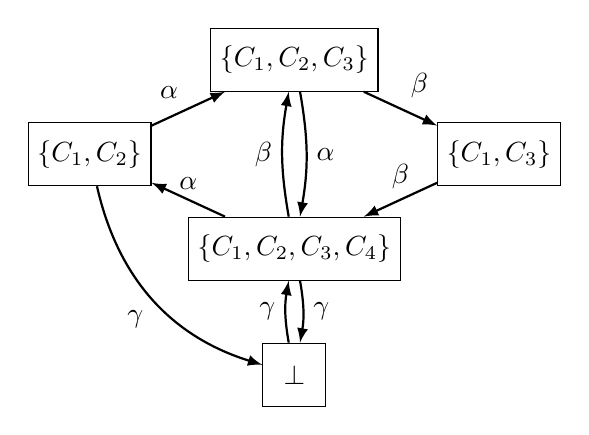
\begin{tikzpicture} [scale=0.8]
		%		\createstate{s1}{3,2+4}{$\state_1$};
		\path
		(\basex+1.75,	\basey+4.5) 	node[gstate] (c12) 		{$\{\cycle_1, \cycle_2\}$} 		
		(\basex+8.25,	\basey+4.5) 	node[gstate] (c13) 		{$\{\cycle_1, \cycle_3\}$}
		(\basex+5,		\basey+1) 	node[gstate] (cbot) 		{$\notppty$}
		(\basex+5,		\basey+6) 	node[gstate] (c123) 		{$\{\cycle_1, \cycle_2, \cycle_3\}$} 
		(\basex+5,		\basey+3) 	node[gstate] (c1234) 	{$\{\cycle_1, \cycle_2, \cycle_3, \cycle_4\}$} 
		
		;
		
		\path [trans] (c12) edge node [midway, above left] {\action} (c123);
		\path [trans] (c123) edge node [midway, above right] {\actionb} (c13);
		\path [trans] (c13) edge node [midway, above] {\actionb} (c1234);
		\path [bendtrans] (cbot) edge node [midway, left] {\actionc} (c1234);
		\path [bendtrans] (c1234) edge node [midway, right] {\actionc} (cbot);
		\path [bendtrans] (c1234) edge node [midway, left] {\actionb} (c123);
		\path [bendtrans] (c123) edge node [midway, right] {\action} (c1234);
		\path [trans] (c1234) edge node [midway, above] {\action} (c12);
		\path [trans, bend right=30] (c12) edge node [midway,below left] {\actionc} (cbot);		
		
	\end{tikzpicture}
\end{document}
	\end{minipage}
	\caption{\viewNC \viewexactactcycle[0] (left) and \viewN \viewexactactcycle[5] (right)}
	\label{fig:cycleAfterExtact0}  
\end{figure}



\begin{definition}
	Let $\chgph = \chgphtuple$ be \achgphN and $n \in \natnums$. The \viewN \viewexactactcycle is defined by its \grpfctN $\gfctexactactcycle : \states \to \imggrp$ with
	\[
	\state \mapsto \{\cycle \in \cycleset \mid \state \in \cycle, \tilde{\action} \in \cycle, \forall \action \in \cycle : \action = \tilde{\action} \}
	\]
	
	and $\imggrp = \powerset{\cycleset} \cup \remset.$
\end{definition}

The view specializes the view from Definition \ref{def:exactcycleview} in the sense that it additionally requires for all $\cycle \in \gfctexactcycle$ that all actions occurring in the cycle are the same. \redcomment{doubling to above definition?}

\redcomment{NO DISCUSSION IF PREVIOUSLY}

In definition \ref{def:exactcycleview} we stated that little grouping can occur when mapping on the set of cycles in all of which the state is contained. Hence we provide the definition and implemenation of a view that groups states even though their set of cycles is not equal, but there is sufficient similarity in the cycles they are on.

\begin{definition}
	Let $\chgph = \chgphtuple$ be \achgphN and $n \in \natnums$. The \viewN \viewcycleset is defined by its \grpfctN $\gfctcycleset : \states \to \imggrp$ with
	\[
	\state \mapsto \{\smstate \in \states \mid \state, \smstate \in \cycle \in \cycleset\}
	\]
	and $\imggrp = \states \cup \remset.$
\end{definition}

\begin{figure}[h]
	\centering
	\documentclass[tikz,preview]{standalone}
%\usepackage{prelude}

%%%%%%%%%%%%%%%%%%%%%%%%%%%%%%%%%%%% PACKAGES %%%%%%%%%%%%%%%%%%%%%%%%%%%%%%%%%%%%%%%%%%

\usepackage{inputenc,fontenc}
\usepackage[a4paper,margin=3cm]{geometry}
\usepackage[english]{babel}
%\usepackage[german]{babel}
%\usepackage[fixlanguage]{babelbib}


\usepackage{bbold}
\usepackage{amsthm}
\usepackage{amsmath}
\usepackage{amssymb} % doteqdot
\usepackage[dvipsnames]{xcolor}
\usepackage{standalone}
\usepackage{tikz}[mode=buildnew]
\usepackage{cite}
\usepackage{xspace}
\usepackage{relsize}
\usepackage{mathtools} % mathclap
%\usepackage{MnSymbol}
\usepackage{hyperref}
\usepackage{url}
\usepackage{listings} % for code
\usepackage[T1]{fontenc} %<
\hypersetup{
	colorlinks,
	citecolor=black,
	filecolor=black,
	linkcolor=black,
	urlcolor=black
}
\usepackage{pgfplots}
\pgfplotsset{compat=1.18}
%\usepackage{courier} %% Sets font for listing as Courier. But also for url and texttt!
\usepackage{listings, xcolor}
\usepackage{graphicx}
\usepackage{subcaption}

\usetikzlibrary{calc}
%\usepackage{xparse} % \newDocumentCommand for multiple optional arguments
%\usepackage{titlecaps}



%%%%%%%%%%%%%%%%%%%%%%%%%%%%%%%%%%%% THEOREMSTYLES %%%%%%%%%%%%%%%%%%%%%%%%%%%%%%%%%%

\theoremstyle{definition}
\newtheorem{definition}{Definition}[section]
\newtheorem{exmp}{Beispiel}[section]
%\AfterEndEnvironment{definition}{\noindent\ignorespaces}

\theoremstyle{theorem}
\newtheorem{theorem}{Satz}[section]
\newtheorem{proposition}{Proposition}[section]
%\AfterEndEnvironment{theorem}{\noindent\ignorespaces}

\theoremstyle{korollary}
\newtheorem{korollary}{Korollar}[section]
%\AfterEndEnvironment{korollary}{\noindent\ignorespaces}


\tikzset{
	mstate/.style={draw, circle, minimum size=.94cm}, 
	gstate/.style={draw, rectangle, minimum size=.8cm},
	varstate/.style={draw,rectangle, rounded corners, minimum size=1}, 
	trans/.style={draw, ->, thick},
	bendtrans/.style={draw, ->, thick, bend left=10},
	bendtransr/.style={draw, ->, thick, bend right=10},
	init/.style={initial, initial distance=6pt, initial text=},
	every loop/.style={min distance=5pt, looseness=8},
	>=latex
}
\usetikzlibrary{automata,positioning}

%auto shift/.style={auto=right,->,
%	to path={ let \p1=(\tikztostart),\p2=(\tikztotarget),
%		\n1={atan2(\y2-\y1,\x2-\x1)},\n2={\n1+180}
%		in ($(\tikztostart.{\n1})!1mm!270:(\tikztotarget.{\n2})$) -- 
%		($(\tikztotarget.{\n2})!1mm!90:(\tikztostart.{\n1})$) \tikztonodes}},

%%%%%%%%%%%%%%%%%%%%%%%%%%%%%%%%%%% MY MACROS %%%%%%%%%%%%%%%%%%%%%%%%%%%%%%%%%%%%%%%%%
%formatting
\newcommand{\comment}[2]{{\color{#1}#2}}
\newcommand{\redcomment}[1]{{\color{red}#1}}
\newcommand{\purpcomment}[1]{{\color{pink}#1}}
\newcommand{\bluecomment}[1]{{\color{blue}#1}}
\newcommand{\mt}[1]{\ensuremath{{#1}}\xspace}
\newcommand{\mynewcommand}[2]{\newcommand{#1}{\mt{#2}}} %% currently not used becaue of ide highlighting
\newcommand{\arr}{\mt{\to}}

%model checking terms
\newcommand{\mimicrel}{\mt{\mathcal{R}}}
\newcommand{\bisimeq}{\mt{\;\!\sim\;\!}}
\newcommand{\simorder}{\mt{\;\!\preceq\;\!}}
\newcommand{\simequiv}{\mt{\;\!\simeq\;\!}} %command already defined
\newcommand{\relts}{\mt{\;\!\bullet_{_{\tiny{TS}}}\;\!}}
\newcommand{\rel}{\mt{\;\!\bullet\;\!}}

%own names
\newcommand{\nm}[1]{#1\xspace}
\newcommand{\mdpN}{\nm{MDP}}
\newcommand{\mdpsN}{\nm{MDPs}}
\newcommand{\viewN}{\nm{view}}
\newcommand{\viewNC}{\nm{View}}
\newcommand{\viewsN}{\nm{views}}
\newcommand{\viewsNC}{\nm{Views}}
\newcommand{\grpfctsubN}{\nm{detached grouping function}}
\newcommand{\grpfctsubNC}{\nm{detached grouping function}}
\newcommand{\grpfctsubNCC}{\nm{Detached Grouping Function}}
\newcommand{\grpfctN}{\nm{grouping function}}
\newcommand{\grpfctNC}{\nm{Grouping function}}
\newcommand{\grpfctNCC}{\nm{Grouping Function}}
\newcommand{\grpfctsN}{\nm{grouping functions}}
\newcommand{\grpfctsNC}{\nm{Grouping functions}}
\newcommand{\grpfctsNCC}{\nm{Grouping Functions}}
\newcommand{\stmimicN}{\nm{state-mimic}}
\newcommand{\stmimicsN}{\nm{state-mimics}}
\newcommand{\stmimickingN}{\nm{state-mimicking}}
\newcommand{\stmimickedN}{\nm{state-mimicked}}
%\newcommand{\chosenphtypeNCC}{\nm{Transition System}}
%\newcommand{\chgphNC}{\nm{Transition system}}
%\newcommand{\chgphN}{\nm{transition system}}
%\newcommand{\chgphsNCC}{\nm{Transition Systems}}
%\newcommand{\chgphsNC}{\nm{Transition systems}}
%\newcommand{\chgphsN}{\nm{transition systems}}
\newcommand{\chgphNCC}{\nm{MDP}}
\newcommand{\chgphNC}{\nm{MDP}}
\newcommand{\chgphN}{\nm{MDP}}
\newcommand{\achgphN}{\nm{an MDP}}
\newcommand{\chgphsNCC}{\nm{MDPs}}
\newcommand{\chgphsNC}{\nm{MDPs}}
\newcommand{\chgphsN}{\nm{MDPs}}
\newcommand{\parllcompN}{\nm{parallel composition}}
\newcommand{\parllcompNC}{\nm{Parallel composition}}
\newcommand{\parllcompNCC}{\nm{Parallel Composition}}
\newcommand{\parllcompsN}{\nm{parallel compositions}}
\newcommand{\parllcompsNC}{\nm{Parallel compositions}}
\newcommand{\parllcompsNCC}{\nm{Parallel Compositions}}
\newcommand{\sccN}{\nm{SCC}}
\newcommand{\sccsN}{\nm{SCCs}}
\newcommand{\bsccN}{\nm{BSCC}}
\newcommand{\bsccsN}{\nm{BSCCs}}
\newcommand{\jgrapht}{\nm{jGraphtT}}

\newcommand{\outactident}{\nm{OutActionsIdent}}

%names
\newcommand{\iffN}{\nm{if and only if}}
\newcommand{\tsN}{\nm{TS}}

%% outactions identical
\newcommand{\outactidentstrong}{\nm{strong}}
\newcommand{\outactidentweak}{\nm{weak}}

% CORE DEFINITIONS
\newcommand{\grpfct}[1][\viewppty]{\mt{F_{#1}}}
\newcommand{\grpfctsub}[1][\viewppty]{\mt{\tilde{F}_{#1}}}
%\newcommand{\grpfctimg}[1]{\mt{{\grpfct}[{#1}]}}
%\newcommand{\fctimg}[2]{\mt{{#1}[{#2}]}}
\newcommand{\eqrelview}{\mt{R}}
\newcommand{\eqclassv}[1][\state]{\mt{\eqclass{#1}{\eqrelview}}}
\newcommand{\eqclasssetv}[1][\states]{\mt{{#1}/\eqrelview}} %OLD: \bigcup_{\state \in \states} \eqclassv
\newcommand{\viewid}{\mt{\mdp}}
\newcommand{\view}[1][\viewppty]{\mt{\viewid_{#1}}}
\newcommand{\imggrp}{\mt{\arbset}}
\newcommand{\imggrpsub}{\mt{X}}
\newcommand{\viewppty}{\mt{\theta}}
\newcommand{\pll}{\mt{\;\!\pllpure\;\!}}
\newcommand{\pllrev}{\mt{\pllpure^{-1}}}
\newcommand{\pllpure}{\mt{||}}
\newcommand{\compselectset}{\mt{Z}}
\newcommand{\compselectpure}{\mt{\pllpure_\compselectset}}
\newcommand{\compselect}{\mt{\;\pllpure_\compselectset\;}}
\newcommand{\remstates}{\mt{\bigcup_{\state \in \states \setminus \states_1}\{\{\state\}\}}}
\newcommand{\nogroupstates}[1][\states_2]{\mt{\bigcup_{\state \in \states \setminus {#1}}\{\{\state\}\}}}
\newcommand{\remelem}{\mt{\bullet}}
\newcommand{\nogroupset}{\mt{\xi}}
\newcommand{\remset}{\mt{\{\remelem\}}}
\newcommand{\gfctpll}{\mt{\grpfct[\pll]}}
\newcommand{\group}{\mt{\top}}
\newcommand{\imggrpbinview}{\mt{\{\remelem, \notppty\}}}
\newcommand{\viewappset}{\mt{\tilde{\states}}}
\newcommand{\hasppty}{\mt{\top}}
\newcommand{\notppty}{\mt{\bot}}
\newcommand{\disregardelem}{\mt{\Delta}}
\newcommand{\disregardelements}{\mt{{\disregardelem_1, \dots, \disregardelem_n}}}



%\newcommand{\mdp}{def}\mdp
%\newcommand{\mdpdef}



% EXAMPLE VIEWS
\newcommand{\pptyatomicprops}{\mt{\atomicprops}}
\newcommand{\pptyinitstates}{\mt{\initstates}}
\newcommand{\pptyinactsetsize}{\mt{|\inacts(\state)|}}
\newcommand{\pptyhasoutact}{\mt{\exists\outact}}
\newcommand{\pptyminoutact}[2]{\mt{#1\leq#2}}
\newcommand{\pptymaxoutact}[2]{\mt{#2\leq#1}}
\newcommand{\pptyspanoutact}[3]{\mt{#1\leq#2\leq#3}}
\newcommand{\pptyoutactsetsize}{\mt{|\outacts(\state)|}}
\newcommand{\pptyoutactsingle}{\mt{|\outacts(\state)|_1}}
\newcommand{\pptystrongoutactident}{\mt{\outacts(\state)_=}}
\newcommand{\pptyweakoutactident}{\mt{\outacts(\state)_\approx}}
\newcommand{\pptyhasinact}{\mt{\exists\inact}}
\newcommand{\pptymininact}[2]{\mt{#1\leq#2}}
\newcommand{\pptymaxinact}[2]{\mt{#2\leq#1}}
\newcommand{\pptyspaninact}[3]{\mt{#1\leq#2\leq#3}}
\newcommand{\pptyinactsingle}{\mt{|\inacts(\state)|_1}}
\newcommand{\pptystronginactident}{\mt{\inacts(\state)_=}}
\newcommand{\pptyweakinactident}{\mt{\inacts(\state)_\approx}}
\newcommand{\pptyparamvalueseq}{\mt{\var = \varval}}
\newcommand{\pptyparamvaluesneq}{\mt{\var \neq \varval}}
\newcommand{\pptyparamdnf}{\mt{VarDNF}}
\newcommand{\pptyparamcnf}{\mt{VarCNF}}
\newcommand{\pptyparamvalueseqopt}{\mt{\var = \varval}}
\newcommand{\pptyparamvalident}{\mt{Var:\varval}}
\newcommand{\pptydistance}{\mt{\distpath}}
\newcommand{\pptydistancerev}{\mt{\distpathrev}}
\newcommand{\pptydistancebi}{\mt{\distpathbi}}
\newcommand{\pptyhascycle}{\mt{\exists\cycle}}
\newcommand{\pptyexactactcycle}{\mt{\{\cycle_{\action,n}\}}}
\newcommand{\pptycycleset}{\mt{\cup{\{\state\}_\cycle}}}
\newcommand{\pptyexactcycle}{\mt{\{\cycle_n\}}}
\newcommand{\pptyscc}{\mt{scc}}
\newcommand{\pptybscc}{\mt{bscc}}
\newcommand{\pptyprop}{\mt{\redcomment{?}}}
\newcommand{\pptyident}{id}


\newcommand{\gfctatomicprops}{\mt{\grpfct[\pptyatomicprops]}}
\newcommand{\gfctinitstates}{\mt{\grpfct[\pptyinitstates]^\hasppty}}
\newcommand{\gfcthasoutaction}{\mt{\grpfct[\pptyhasoutact]^\hasppty}}
\newcommand{\gfctminoutaction}{\mt{\grpfct[\pptyminoutact{\numoutact}{\outact}]^\hasppty}}
\newcommand{\gfctmaxoutaction}{\mt{\grpfct[\pptymaxoutact{\numoutact}{\outact}]^\hasppty}}
\newcommand{\gfctspanoutaction}{\mt{\grpfct[\pptyspanoutact{\numoutactb}{\outact}{\numoutact}]^\hasppty}}
\newcommand{\gfctoutactsetsize}{\mt{\grpfct[\pptyoutactsetsize]}}
\newcommand{\gfctoutactsingle}{\mt{\grpfct[\pptyoutactsingle]^\notppty}}
\newcommand{\gfctstrongoutactident}{\mt{\grpfct[\pptystrongoutactident]}}
\newcommand{\gfctweakoutactident}{\mt{\grpfct[\pptyweakoutactident]}}
\newcommand{\gfcthasinaction}{\mt{\grpfct[\pptyhasinact]^\hasppty}}
\newcommand{\gfctmininaction}{\mt{\grpfct[\pptymininact{\numinact}{\inact}]^\hasppty}}
\newcommand{\gfctmaxinaction}{\mt{\grpfct[\pptymaxinact{\numinact}{\inact}]^\hasppty}}
\newcommand{\gfctspaninaction}{\mt{\grpfct[\pptyspaninact{\numinactb}{\inact}{\numinact}]^\hasppty}}
\newcommand{\gfctinactsetsize}{\mt{\grpfct[\pptyinactsetsize]}}
\newcommand{\gfctinactsingle}{\mt{\grpfct[\pptyinactsingle]^\notppty}}
\newcommand{\gfctstronginactident}{\mt{\grpfct[\pptystronginactident]}}
\newcommand{\gfctweakinactident}{\mt{\grpfct[\pptyweakinactident]}}
\newcommand{\gfctparamvalueseq}{\mt{\grpfct[\pptyparamvalueseq]^\hasppty}}
\newcommand{\gfctparamvaluesneq}{\mt{\grpfct[\pptyparamvaluesneq]^\hasppty}}
\newcommand{\gfctparamdnf}{\mt{\grpfct[\pptyparamdnf]^\hasppty}}
\newcommand{\gfctparamcnf}{\mt{\grpfct[\pptyparamcnf]^\hasppty}}
\newcommand{\gfctparamvalueseqopt}{\mt{\pptyparamvalueseqopt}}
\newcommand{\gfctparamvalident}{\mt{\grpfct[\pptyparamvalident]}}
\newcommand{\gfctdistance}{\mt{\grpfct[\pptydistance]}}
\newcommand{\gfctdistancerev}{\mt{\grpfct[\pptydistancerev]}}
\newcommand{\gfctdistancebi}{\mt{\grpfct[\pptydistancebi]}}
\newcommand{\gfcthascycle}{\mt{\grpfct[\pptyhascycle]}}
\newcommand{\gfctexactcycle}{\mt{\grpfct[\pptyexactcycle]}}
\newcommand{\gfctcycleset}{\mt{\grpfct[\pptycycleset]}}
\newcommand{\gfctexactactcycle}{\mt{\grpfct[\pptyexactactcycle]}}
\newcommand{\gfctscc}{\mt{\grpfct[\pptyscc]}}
\newcommand{\gfctbscc}{\mt{\grpfct[\pptybscc]}}
\newcommand{\gfctprop}{\mt{\grpfct[\pptyprop]}}
\newcommand{\gfctident}{\mt{\grpfct[\pptyident]}}

\newcommand{\gfctsubatomicprops}{\mt{\grpfctsub[\pptyatomicprops]}}
\newcommand{\gfctsubinitstates}{\mt{\grpfctsub[\pptyinitstates]^\hasppty}}
\newcommand{\gfctsubhasoutaction}{\mt{\grpfctsub[\pptyhasoutact]^\hasppty}}
\newcommand{\gfctsubminoutaction}{\mt{\grpfctsub[\pptyminoutact{\numoutact}{\outact}]^\hasppty}}
\newcommand{\gfctsubmaxoutaction}{\mt{\grpfctsub[\pptymaxoutact{\numoutact}{\outact}]^\hasppty}}
\newcommand{\gfctsubspanoutaction}{\mt{\grpfctsub[\pptyspanoutact{\numoutactb}{\outact}{\numoutact}]^\hasppty}}
\newcommand{\gfctsuboutactsetsize}{\mt{\grpfctsub[\pptyoutactsetsize]}}
\newcommand{\gfctsuboutactsingle}{\mt{\grpfctsub[\pptyoutactsingle]^\notppty}}
\newcommand{\gfctsubstrongoutactident}{\mt{\grpfctsub[\pptystrongoutactident]^\hasppty}}
\newcommand{\gfctsubweakoutactident}{\mt{\grpfctsub[\pptyweakoutactident]^\hasppty}}
\newcommand{\gfctsubhasinaction}{\mt{\grpfctsub[\pptyhasinact]}}
\newcommand{\gfctsubmininaction}{\mt{\grpfctsub[\pptymininact{\numinact}{\inact}]}}
\newcommand{\gfctsubmaxinaction}{\mt{\grpfctsub[\pptymaxinact{\numinact}{\inact}]}}
\newcommand{\gfctsubspaninaction}{\mt{\grpfctsub[\pptyspaninact{\numinactb}{\inact}{\numinact}]}}
\newcommand{\gfctsubinactsetsize}{\mt{\grpfctsub[\pptyinactsetsize]^\hasppty}}
\newcommand{\gfctsubinactsingle}{\mt{\grpfctsub[\pptyinactsingle]^\notppty}}
\newcommand{\gfctsubstronginactident}{\mt{\grpfctsub[\pptystronginactident]}}
\newcommand{\gfctsubweakinactident}{\mt{\grpfctsub[\pptyweakinactident]}}
\newcommand{\gfctsubparamvalueseq}{\mt{\grpfctsub[\pptyparamvalueseq]^\hasppty}}
\newcommand{\gfctsubparamvaluesneq}{\mt{\grpfctsub[\pptyparamvaluesneq]^\hasppty}}
\newcommand{\gfctsubparamdnf}{\mt{\grpfctsub[\pptyparamdnf]^\hasppty}}
\newcommand{\gfctsubparamcnf}{\mt{\grpfctsub[\pptyparamcnf]^\hasppty}}
\newcommand{\gfctsubparamvalueseqopt}{\mt{\pptyparamvalueseqopt}}
\newcommand{\gfctsubparamvalident}{\mt{\grpfctsub[\pptyparamvalident]}}
\newcommand{\gfctsubdistance}{\mt{\grpfctsub[\pptydistance]}}
\newcommand{\gfctsubdistancerev}{\mt{\grpfctsub[\pptydistancerev]}}
\newcommand{\gfctsubdistancebi}{\mt{\grpfctsub[\pptydistancebi]}}
\newcommand{\gfctsubhascycle}{\mt{\grpfctsub[\pptyhascycle]^\hasppty}}
\newcommand{\gfctsubexactcycle}{\mt{\grpfctsub[\pptyexactcycle]}}
\newcommand{\gfctsubcycleset}{\mt{\grpfctsub[\pptycycleset]}}
\newcommand{\gfctsubexactactcycle}{\mt{\grpfctsub[\pptyexactactcycle]}}
\newcommand{\gfctsubscc}{\mt{\grpfctsub[\pptyscc]}}
\newcommand{\gfctsubbscc}{\mt{\grpfctsub[\pptybscc]}}
\newcommand{\gfctsubprop}{\mt{\grpfctsub[\pptyprop]}}
\newcommand{\gfctsubident}{\mt{\grpfctsub[\pptyident]}}


\newcommand{\viewatomicprops}{\mt{\view[\pptyatomicprops]}}
\newcommand{\viewinitstates}{\mt{\view[\pptyinitstates]^\hasppty}}
\newcommand{\viewhasoutaction}{\mt{\view[\pptyhasoutact]^\hasppty}}
\newcommand{\viewminoutaction}{\mt{\view[\pptyminoutact{\numoutact}{\outact}]^\hasppty}}
\newcommand{\viewmaxoutaction}{\mt{\view[\pptymaxoutact{\numoutact}{\outact}]^\hasppty}}
\newcommand{\viewspanoutaction}{\mt{\view[\pptyspanoutact{\numoutactb}{\outact}{\numoutact}]^\hasppty}}
\newcommand{\viewoutactsetsize}{\mt{\view[\pptyoutactsetsize]}}
\newcommand{\viewoutactsingle}{\mt{\view[\pptyoutactsingle]^\notppty}}
\newcommand{\viewstrongoutactident}{\mt{\view[\pptystrongoutactident]}}
\newcommand{\viewweakoutactident}{\mt{\view[\pptyweakoutactident]}}
\newcommand{\viewhasinaction}{\mt{\view[\pptyhasinact]^\hasppty}}
\newcommand{\viewmininaction}{\mt{\view[\pptymininact{\numinact}{\inact}]^\hasppty}}
\newcommand{\viewmaxinaction}{\mt{\view[\pptymaxinact{\numinact}{\inact}]^\hasppty}}
\newcommand{\viewspaninaction}{\mt{\view[\pptyspaninact{\numinactb}{\inact}{\numinact}]^\hasppty}}
\newcommand{\viewinactsetsize}{\mt{\view[\pptyinactsetsize]}}
\newcommand{\viewinactsingle}{\mt{\view[\pptyinactsingle]^\notppty}}
\newcommand{\viewstronginactident}{\mt{\view[\pptystronginactident]}}
\newcommand{\viewweakinactident}{\mt{\view[\pptyweakinactident]}}
\newcommand{\viewparamvalueseq}{\mt{\view[\pptyparamvalueseq]}}
\newcommand{\viewparamvaluesneq}{\mt{\view[\pptyparamvaluesneq]}}
\newcommand{\viewparamdnf}{\mt{\view[\pptyparamdnf]^\hasppty}}
\newcommand{\viewparamcnf}{\mt{\view[\pptyparamcnf]^\hasppty}}
\newcommand{\viewparamvalueseqopt}{\mt{\pptyparamvalueseqopt}}
\newcommand{\viewparamvalident}{\mt{\view[\pptyparamvalident]}}
\newcommand{\viewdistance}{\mt{\view[\pptydistance]}}
\newcommand{\viewdistancerev}{\mt{\view[\pptydistancerev]}}
\newcommand{\viewdistancebi}{\mt{\view[\pptydistancebi]}}
\newcommand{\viewhascycle}{\mt{\view[\pptyhascycle]}}
\newcommand{\viewexactcycle}{\mt{\view[\pptyexactcycle]}}
\newcommand{\viewcycleset}{\mt{\view[\pptycycleset]}}
\newcommand{\viewexactactcycle}{\mt{\view[\pptyexactactcycle]}}
\newcommand{\viewscc}{\mt{\view[\pptyscc]}}
\newcommand{\viewbscc}{\mt{\view[\pptybscc]}}
\newcommand{\viewprop}{\mt{\view[\pptyprop]}}
\newcommand{\viewident}{\mt{\view[\pptyident]}}

%\newcommand{\viewatomicprops}{\mt{\view[\atomicprops]}}
%\newcommand{\viewinitstates}{\mt{\view[\initstates]}}
%\newcommand{\viewhasoutaction}{\mt{\view[\pptyhasoutact]}}
%\newcommand{\viewminoutaction}{\mt{\view[\pptyminoutact{\numoutact}{\outact}]}}
%\newcommand{\viewmaxoutaction}{\mt{\view[\pptymaxoutact{\numoutact}{\outact}]}}
%\newcommand{\viewspanoutaction}{\mt{\view[\pptyspanoutact{\numoutactb}{\outact}{\numoutact}]}}
%\newcommand{\viewoutactsetsize}{\mt{\view[\pptyoutactsetsize]}}
%\newcommand{\viewoutactsingle}{\mt{\view[\pptyoutactsingle]}}
%\newcommand{\viewstrongoutactident}{\mt{\view[\outacts(\state)_=]}}
%\newcommand{\viewweakoutactident}{\mt{\view[\outacts(\state)_\approx]}}
%\newcommand{\viewhasinaction}{\mt{\view[\pptyhasinact]}}
%\newcommand{\viewmininaction}{\mt{\view[\pptymininact{\numinact}{\inact}]}}
%\newcommand{\viewmaxinaction}{\mt{\view[\pptymaxinact{\numinact}{\inact}]}}
%\newcommand{\viewspaninaction}{\mt{\view[\pptyspaninact{\numinactb}{\inact}{\numinact}]}}
%\newcommand{\viewinactsetsize}{\mt{\view[\pptyinactsetsize]}}
%\newcommand{\viewinactsingle}{\mt{\view[\pptyinactsingle]}}
%\newcommand{\viewstronginactident}{\mt{\view[\inacts(\state)_=]}}
%\newcommand{\viewweakinactident}{\mt{\view[\inacts(\state)_\approx]}}
%\newcommand{\viewparamvalueseq}{\mt{\view[\var = \varval]}}
%\newcommand{\viewparamvaluesneq}{\mt{\view[\var \neq \varval]}}
%\newcommand{\viewparamdnf}{\mt{\view[VarDNF]}}
%\newcommand{\viewparamcnf}{\mt{\view[VarCNF]}}
%\newcommand{\viewparamvalident}{\mt{\view[\pptyparamvalident]}}
%\newcommand{\viewdistance}{\mt{\view[\pptydistance]}}
%\newcommand{\viewhascycle}{\mt{\view[\exists\cycle]}}
%\newcommand{\viewexactcycle}{\mt{\view[\pptyexactcycle]}}
%\newcommand{\viewcycleset}{\mt{\view[\pptycycleset]}}
%\newcommand{\viewexactactcycle}{\mt{\view[\pptyexactactcycle]}}
%\newcommand{\viewscc}{\mt{\view[scc]}}
%\newcommand{\viewbscc}{\mt{\view[bscc]}}

%actions
\newcommand{\numoutact}{\mt{n}}
\newcommand{\numoutactb}{\mt{m}}
\newcommand{\numinact}{\mt{n}}
\newcommand{\numinactb}{\mt{m}}

\newcommand{\predmaxoutact}[1][\numoutact]{\mt{Q_{\outact\leq#1}(\state,\state_1, \dots, \state_{#1+1})}}
\newcommand{\predminoutact}[1][\numoutact]{\mt{Q_{#1\leq\outact}(\state,\state_1, \dots, \state_{#1})}}
\newcommand{\formoutact}[1][\state]{\mt{C_{#1,\outact}}}
\newcommand{\predmaxinact}[1][\numinact]{\mt{Q_{\inact\leq#1}(\state,\state_1, \dots, \state_{#1+1})}}
\newcommand{\predmininact}[1][\numinact]{\mt{Q_{#1\leq\inact}(\state,\state_1, \dots, \state_{#1})}}

\newcommand{\outact}[1][\action]{\mt{\overrightarrow{#1}}}
\newcommand{\outacts}{\mt{\overrightarrow{\actions}}}
\newcommand{\inact}{\mt{\overleftarrow{\action}}}
\newcommand{\inacts}[1][\action]{\mt{\overleftarrow{#1}}}

%%Parameters
\newcommand{\vars}[1][\mdp]{\mt{V\!ar_{#1}}}
\newcommand{\var}{\mt{x}}
\newcommand{\varstate}[1][]{\mt{\var_{\state#1}}}
\newcommand{\varval}{\mt{a}}
\newcommand{\vareval}[1][\mdp]{\mt{V\!arEval_{#1}}}
\newcommand{\varevalimg}[1][\mdp]{\mt{\vareval[#1][\states,\vars]}}
\newcommand{\varevalimgset}{\mt{\arbset}}
\newcommand{\someparam}{\mt{\tilde{x}}}
\newcommand{\eqorneq}{\mt{\;\doteqdot\;}}
\newcommand{\varstyle}[2]{\mt{\langle#1,#2\rangle}}




%\makeatletter
%\newcommand{\overleftrightsmallarrow}{\mathpalette{\overarrowsmall@\leftrightarrowfill@}}
%\newcommand{\overrightsmallarrow}{\mathpalette{\overarrowsmall@\rightarrowfill@}}
%\newcommand{\overleftsmallarrow}{\mathpalette{\overarrowsmall@\leftarrowfill@}}
%\newcommand{\overarrowsmall@}[3]{%
%	\vbox{%
%		\ialign{%
%			##\crcr
%			#1{\smaller@style{#2}}\crcr
%			\noalign{\nointerlineskip}%
%			$\m@th\hfil#2#3\hfil$\crcr
%		}%
%	}%
%}
%\def\smaller@style#1{%
%	\ifx#1\displaystyle\scriptstyle\else
%	\ifx#1\textstyle\scriptstyle\else
%	\scriptscriptstyle
%	\fi
%	\fi
%}
%\makeatother
%\newcommand{\te}[1]{\overleftrightsmallarrow{#1}}

% Distance
\newcommand{\fctdist}{\mt{distance}}
\newcommand{\fctdistdefault}{\mt{\fctdist(\chgph, \smstates, \grandist)}}
\newcommand{\distval}{\mt{d}}
\newcommand{\grandist}{\mt{n}}
\let\path\oldpath
\newcommand{\path}{\mt{P}}
\newcommand{\pathbi}{\mt{\bar{\path}}}
\newcommand{\pathsecfull}{\mt{(\state_0, \action_0, \state_1, \action_1, \dots, \action_{n}, \state_{n+1})}}
\newcommand{\lenpath}{\mt{len}}
\newcommand{\pfirst}{\mt{first}}
\newcommand{\plast}{\mt{last}}
\newcommand{\pathset}{\mt{\path_\chgph}}
\newcommand{\pathbiset}{\mt{\pathbi_\chgph}}
\newcommand{\distpath}{\mt{\overrightarrow{dist}}}
\newcommand{\distpathrev}{\mt{\overleftarrow{dist}}}
\newcommand{\distpathbi}{\mt{\overline{dist}}}
%Cycles
\newcommand{\cyclesecfull}{\mt{(\state_0, \action_0, \state_1, \action_1, \dots, \action_{n-1}, \state_0)}}
\newcommand{\fctfindcycles}{\mt{findCycles}}
\newcommand{\cycle}{\mt{C}}
\newcommand{\cycleset}{\mt{\cycle_{\mdp, n}}}
\newcommand{\lencycle}{\mt{len}}
% strongly connected components
\newcommand{\scc}{\mt{T}}
\newcommand{\setscc}{\mt{SCC_{\chgph,n}}}
\newcommand{\setbscc}{\mt{BSCC_{\chgph,n}}}

% properties
\newcommand{\propfct}{\mt{f}}

% all Systems
\newcommand{\chgph}{\mt{\mdp}}
\newcommand{\chgphtuple}{\mt{\mdptuple}}
\newcommand{\chgphtupledist}{\mt{\mdptupledist}}

\newcommand{\states}{\mt{S}}
\newcommand{\actions}{\mt{Act}}
\newcommand{\atomicprops}{\mt{AP}}
\newcommand{\labelingfct}{\mt{L}}
\newcommand{\init}{\mt{\initdistrib}} % use MDP % refers to the underlying set
\newcommand{\trans}{\mt{\probtfunc}} % use MDP % refers to the underlying set
\newcommand{\smstates}{\mt{\tilde{\states}}}


\newcommand{\state}{\mt{s}}
\newcommand{\action}{\mt{\alpha}}
\newcommand{\actionb}{\mt{\beta}}
\newcommand{\actionc}{\mt{\gamma}}
\newcommand{\smstate}{\mt{\tilde{\state}}}



% transition sysstems
\newcommand{\ts}{\mt{TS}}
\newcommand{\transitionrel}{\mt{\longrightarrow}}
\newcommand{\initstates}{\mt{I}}
\newcommand{\transitionsystem}{\mt
	{(\states, \actions, \transitionrel, \initstates, \atomicprops, \labelingfct)}
}
\newcommand{\tstupledist}{\mt{(\states', \actions',\transitionrel', \initstates', \labelingfct')}}


%Markov chains and MDP
\newcommand{\mdp}{\mt{\autm}}
\newcommand{\mdptuple}{\mt{(\states, \actions, \probtfunc, \initdistrib, \atomicprops, \labelingfct)}}
\newcommand{\mdptupledist}{\mt{(\states', \actions', \probtfunc', \initdistrib', \atomicprops', \labelingfct')}}
\newcommand{\autm}{\mt{\mathcal{M}}}
\newcommand{\probtfunc}{\mt{\textbf{P}}}
\newcommand{\initdistrib}{\mt{\iota_{init}}}


%maths
\newcommand{\powerset}[1]{\mt{\mathcal{P}(#1)}}
\newcommand{\eqclass}[2]{\mt{[#1]_{#2}}}%{\mt{#1 / #2}}
\newcommand{\impr}{\mt{\hspace{3mm}\Rightarrow\hspace{2mm}}}
\newcommand{\impl}{\mt{\hspace{3mm}\Leftarrow\hspace{2mm}}}
\newcommand{\natnums}{\mt{\mathbb{N}}} 
\newcommand{\realnums}{\mt{\mathbb{R}}}
\newcommand{\intmodn}[1][n]{\mt{\mathbb{Z}_{#1}}}
\newcommand{\arbset}{\mt{M}}
\newcommand{\bigsum}[2][]{\mt{\mathlarger{\sum}_{#2}^{#1}}}
\newcommand{\bbigsum}[2][]{\mt{\mathlarger{\mathlarger{\sum}}_{#2}^{#1}}}
\newcommand{\invimage}[2]{#1^{\mt{-1}(#2)}}
\newcommand{\img}{\mt{Img}}
\newcommand{\cond}{\mt{\,|\,}}

%tickz
%% \definecolor{darkred}{RGB}{196, 42, 42}

%implementation
\newcommand{\pmcvis}{\nm{PMC-Vis}}



\begin{document}
	\newcommand{\basex}{0}
	\newcommand{\basey}{0}
	\newcommand{\createstate}[3]{\node[draw, circle, minimum size=1cm] (#1) at (#2) {#3}}
	
	
	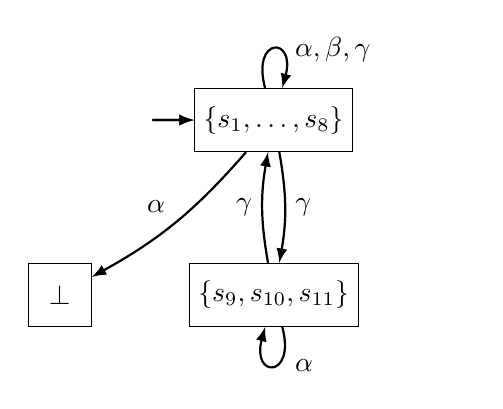
\begin{tikzpicture} [scale=2.5, every initial by arrow/.style={thick}]
		
		
		\path
		(\basex,		\basey) 		node[gstate,init, initial left] (c1) 	{$\{\state_1, \dots, \state_8\}$} 
		
		;
		
		
		\node[gstate,below=40pt of c1] 			(c2) 	{$\{\state_9, \state_{10}, \state_{11}\}$};
		\node[gstate,left=35pt of c2] 	 	(cbot) {$\notppty$};
		\node[right=35pt of c2] {};
		
		
		\path [bendtrans] 	(c1) 	edge node [midway,right]	{$\actionc$} 		(c2);		
		\path [bendtrans] 	(c1) 	edge node [midway,above left]	{$\action$} 		(cbot);				
		\path [bendtrans] 	(c2) 	edge node [midway,left]	{$\actionc$} 		(c1);		
		
		\path [trans] (c1)	edge [loop above] node [midway, right=4pt] {$\action, \actionb, \actionc$}(c1);
		\path [trans] (c2)	edge [loop below] node [midway, right=4pt] {$\action$} (c2);
		
		
	\end{tikzpicture}
\end{document}
	\caption{Simplified representation of the \viewN \viewcycleset on \mdp from Figure \ref{fig:cyclesBefore}} 
	\label{fig:cycleAfterSet0}  
\end{figure}


Each state is mapped to the set of states resulting from joing the state sets of all the cycles the state is on. 

\subsubsection{Strongly Connected Components}
Strongly connect components (\sccN) are of major importance in model checking \redcomment{I think so because I found the terms many times in the book. Remaining question: really? why?}
Therefore it is feasible to consider a view utilizing strongly connected components. Deviating from most definitions we will define \sccN not as a subgraph but only as the set of its nodes. Moreover the definition is written in the terms of \achgphN.

\begin{definition}
	Let $\chgph = \chgphtuple$ be \achgphN. A set $\scc \subseteq \states$ is called \emph{strongly connected component} if for all $\state, \state' \in \scc$ either it holds
	\[
		\exists \path \in \pathset : \pfirst(\path) = \state \land \; \plast(\path) = \state'
	\]
	{\centering{or}}
	\[
	 \state = \state'\text{.}
	\]
	
%	\begin{align*}
%			\scc = \{\state_1 \in \states \mid & \; \forall \state' \in \scc : \exists n \in \natnums, \exists \; \! (\state_1, \action_1, \state_2, \action_2 \dots, \state_n, \action_n, \state') \\
%			&\text{ where } (\state_n, \action_n, \state') \in \trans \land \forall i \in \{1, \dots, n-1\} : (\state_i, \action_i, \state_{i+1}) \in \trans \}
%	\end{align*}
%	That is for every state in the set there has to exist a sequence of transitions to every other state of the set. The state itself is always considered a reachable by itself, i.e. there does not need to exist a self loop. In consequence, each state is contained in stronlgy connected component namely at least in the one that only contains the state. 
	\noindent
	The set of all strongly connected components of \chgph is denoted with \setscc.
\end{definition}

Since the strong connection is an equivalence relation the \sccsN are equivalence classes and hence disjoint. To find \sccsN Tarjans algorithm is the classic. In the implementation an improved variant from Gabow is used supplied by the \jgrapht library. \redcomment{CITATION}

\begin{definition}
	Let $\chgph = \chgphtuple$ be \achgphN and $n \in \natnums$. The \viewN \viewscc is defined by its \grpfctN $\gfctscc : \states \to \imggrp$ with
	\[
	\state \mapsto \{\scc \in \setscc \mid \state \in \scc, n \leq |\scc|\}
	\]
	and $\imggrp = \setscc \cup \remset$.
\end{definition}

This view groups all states together that are in the same \sccN. Because \sccsN are disjoint each \state will be mapped to its one and only \sccN. This is because... \redcomment{DISCUSSION OF EQUALITY, EQ CLASSES AND RESULTING STATES MISSING}

\begin{figure}[h]
	\begin{minipage}{.55\textwidth}
		\hspace{5mm}
		\documentclass[tikz,preview]{standalone}
%\usepackage{prelude}

%%%%%%%%%%%%%%%%%%%%%%%%%%%%%%%%%%%% PACKAGES %%%%%%%%%%%%%%%%%%%%%%%%%%%%%%%%%%%%%%%%%%

\usepackage{inputenc,fontenc}
\usepackage[a4paper,margin=3cm]{geometry}
\usepackage[english]{babel}
%\usepackage[german]{babel}
%\usepackage[fixlanguage]{babelbib}


\usepackage{bbold}
\usepackage{amsthm}
\usepackage{amsmath}
\usepackage{amssymb} % doteqdot
\usepackage[dvipsnames]{xcolor}
\usepackage{standalone}
\usepackage{tikz}[mode=buildnew]
\usepackage{cite}
\usepackage{xspace}
\usepackage{relsize}
\usepackage{mathtools} % mathclap
%\usepackage{MnSymbol}
\usepackage{hyperref}
\usepackage{url}
\usepackage{listings} % for code
\usepackage[T1]{fontenc} %<
\hypersetup{
	colorlinks,
	citecolor=black,
	filecolor=black,
	linkcolor=black,
	urlcolor=black
}
\usepackage{pgfplots}
\pgfplotsset{compat=1.18}
%\usepackage{courier} %% Sets font for listing as Courier. But also for url and texttt!
\usepackage{listings, xcolor}
\usepackage{graphicx}
\usepackage{subcaption}

\usetikzlibrary{calc}
%\usepackage{xparse} % \newDocumentCommand for multiple optional arguments
%\usepackage{titlecaps}



%%%%%%%%%%%%%%%%%%%%%%%%%%%%%%%%%%%% THEOREMSTYLES %%%%%%%%%%%%%%%%%%%%%%%%%%%%%%%%%%

\theoremstyle{definition}
\newtheorem{definition}{Definition}[section]
\newtheorem{exmp}{Beispiel}[section]
%\AfterEndEnvironment{definition}{\noindent\ignorespaces}

\theoremstyle{theorem}
\newtheorem{theorem}{Satz}[section]
\newtheorem{proposition}{Proposition}[section]
%\AfterEndEnvironment{theorem}{\noindent\ignorespaces}

\theoremstyle{korollary}
\newtheorem{korollary}{Korollar}[section]
%\AfterEndEnvironment{korollary}{\noindent\ignorespaces}


\tikzset{
	mstate/.style={draw, circle, minimum size=.94cm}, 
	gstate/.style={draw, rectangle, minimum size=.8cm},
	varstate/.style={draw,rectangle, rounded corners, minimum size=1}, 
	trans/.style={draw, ->, thick},
	bendtrans/.style={draw, ->, thick, bend left=10},
	bendtransr/.style={draw, ->, thick, bend right=10},
	init/.style={initial, initial distance=6pt, initial text=},
	every loop/.style={min distance=5pt, looseness=8},
	>=latex
}
\usetikzlibrary{automata,positioning}

%auto shift/.style={auto=right,->,
%	to path={ let \p1=(\tikztostart),\p2=(\tikztotarget),
%		\n1={atan2(\y2-\y1,\x2-\x1)},\n2={\n1+180}
%		in ($(\tikztostart.{\n1})!1mm!270:(\tikztotarget.{\n2})$) -- 
%		($(\tikztotarget.{\n2})!1mm!90:(\tikztostart.{\n1})$) \tikztonodes}},

%%%%%%%%%%%%%%%%%%%%%%%%%%%%%%%%%%% MY MACROS %%%%%%%%%%%%%%%%%%%%%%%%%%%%%%%%%%%%%%%%%
%formatting
\newcommand{\comment}[2]{{\color{#1}#2}}
\newcommand{\redcomment}[1]{{\color{red}#1}}
\newcommand{\purpcomment}[1]{{\color{pink}#1}}
\newcommand{\bluecomment}[1]{{\color{blue}#1}}
\newcommand{\mt}[1]{\ensuremath{{#1}}\xspace}
\newcommand{\mynewcommand}[2]{\newcommand{#1}{\mt{#2}}} %% currently not used becaue of ide highlighting
\newcommand{\arr}{\mt{\to}}

%model checking terms
\newcommand{\mimicrel}{\mt{\mathcal{R}}}
\newcommand{\bisimeq}{\mt{\;\!\sim\;\!}}
\newcommand{\simorder}{\mt{\;\!\preceq\;\!}}
\newcommand{\simequiv}{\mt{\;\!\simeq\;\!}} %command already defined
\newcommand{\relts}{\mt{\;\!\bullet_{_{\tiny{TS}}}\;\!}}
\newcommand{\rel}{\mt{\;\!\bullet\;\!}}

%own names
\newcommand{\nm}[1]{#1\xspace}
\newcommand{\mdpN}{\nm{MDP}}
\newcommand{\mdpsN}{\nm{MDPs}}
\newcommand{\viewN}{\nm{view}}
\newcommand{\viewNC}{\nm{View}}
\newcommand{\viewsN}{\nm{views}}
\newcommand{\viewsNC}{\nm{Views}}
\newcommand{\grpfctsubN}{\nm{detached grouping function}}
\newcommand{\grpfctsubNC}{\nm{detached grouping function}}
\newcommand{\grpfctsubNCC}{\nm{Detached Grouping Function}}
\newcommand{\grpfctN}{\nm{grouping function}}
\newcommand{\grpfctNC}{\nm{Grouping function}}
\newcommand{\grpfctNCC}{\nm{Grouping Function}}
\newcommand{\grpfctsN}{\nm{grouping functions}}
\newcommand{\grpfctsNC}{\nm{Grouping functions}}
\newcommand{\grpfctsNCC}{\nm{Grouping Functions}}
\newcommand{\stmimicN}{\nm{state-mimic}}
\newcommand{\stmimicsN}{\nm{state-mimics}}
\newcommand{\stmimickingN}{\nm{state-mimicking}}
\newcommand{\stmimickedN}{\nm{state-mimicked}}
%\newcommand{\chosenphtypeNCC}{\nm{Transition System}}
%\newcommand{\chgphNC}{\nm{Transition system}}
%\newcommand{\chgphN}{\nm{transition system}}
%\newcommand{\chgphsNCC}{\nm{Transition Systems}}
%\newcommand{\chgphsNC}{\nm{Transition systems}}
%\newcommand{\chgphsN}{\nm{transition systems}}
\newcommand{\chgphNCC}{\nm{MDP}}
\newcommand{\chgphNC}{\nm{MDP}}
\newcommand{\chgphN}{\nm{MDP}}
\newcommand{\achgphN}{\nm{an MDP}}
\newcommand{\chgphsNCC}{\nm{MDPs}}
\newcommand{\chgphsNC}{\nm{MDPs}}
\newcommand{\chgphsN}{\nm{MDPs}}
\newcommand{\parllcompN}{\nm{parallel composition}}
\newcommand{\parllcompNC}{\nm{Parallel composition}}
\newcommand{\parllcompNCC}{\nm{Parallel Composition}}
\newcommand{\parllcompsN}{\nm{parallel compositions}}
\newcommand{\parllcompsNC}{\nm{Parallel compositions}}
\newcommand{\parllcompsNCC}{\nm{Parallel Compositions}}
\newcommand{\sccN}{\nm{SCC}}
\newcommand{\sccsN}{\nm{SCCs}}
\newcommand{\bsccN}{\nm{BSCC}}
\newcommand{\bsccsN}{\nm{BSCCs}}
\newcommand{\jgrapht}{\nm{jGraphtT}}

\newcommand{\outactident}{\nm{OutActionsIdent}}

%names
\newcommand{\iffN}{\nm{if and only if}}
\newcommand{\tsN}{\nm{TS}}

%% outactions identical
\newcommand{\outactidentstrong}{\nm{strong}}
\newcommand{\outactidentweak}{\nm{weak}}

% CORE DEFINITIONS
\newcommand{\grpfct}[1][\viewppty]{\mt{F_{#1}}}
\newcommand{\grpfctsub}[1][\viewppty]{\mt{\tilde{F}_{#1}}}
%\newcommand{\grpfctimg}[1]{\mt{{\grpfct}[{#1}]}}
%\newcommand{\fctimg}[2]{\mt{{#1}[{#2}]}}
\newcommand{\eqrelview}{\mt{R}}
\newcommand{\eqclassv}[1][\state]{\mt{\eqclass{#1}{\eqrelview}}}
\newcommand{\eqclasssetv}[1][\states]{\mt{{#1}/\eqrelview}} %OLD: \bigcup_{\state \in \states} \eqclassv
\newcommand{\viewid}{\mt{\mdp}}
\newcommand{\view}[1][\viewppty]{\mt{\viewid_{#1}}}
\newcommand{\imggrp}{\mt{\arbset}}
\newcommand{\imggrpsub}{\mt{X}}
\newcommand{\viewppty}{\mt{\theta}}
\newcommand{\pll}{\mt{\;\!\pllpure\;\!}}
\newcommand{\pllrev}{\mt{\pllpure^{-1}}}
\newcommand{\pllpure}{\mt{||}}
\newcommand{\compselectset}{\mt{Z}}
\newcommand{\compselectpure}{\mt{\pllpure_\compselectset}}
\newcommand{\compselect}{\mt{\;\pllpure_\compselectset\;}}
\newcommand{\remstates}{\mt{\bigcup_{\state \in \states \setminus \states_1}\{\{\state\}\}}}
\newcommand{\nogroupstates}[1][\states_2]{\mt{\bigcup_{\state \in \states \setminus {#1}}\{\{\state\}\}}}
\newcommand{\remelem}{\mt{\bullet}}
\newcommand{\nogroupset}{\mt{\xi}}
\newcommand{\remset}{\mt{\{\remelem\}}}
\newcommand{\gfctpll}{\mt{\grpfct[\pll]}}
\newcommand{\group}{\mt{\top}}
\newcommand{\imggrpbinview}{\mt{\{\remelem, \notppty\}}}
\newcommand{\viewappset}{\mt{\tilde{\states}}}
\newcommand{\hasppty}{\mt{\top}}
\newcommand{\notppty}{\mt{\bot}}
\newcommand{\disregardelem}{\mt{\Delta}}
\newcommand{\disregardelements}{\mt{{\disregardelem_1, \dots, \disregardelem_n}}}



%\newcommand{\mdp}{def}\mdp
%\newcommand{\mdpdef}



% EXAMPLE VIEWS
\newcommand{\pptyatomicprops}{\mt{\atomicprops}}
\newcommand{\pptyinitstates}{\mt{\initstates}}
\newcommand{\pptyinactsetsize}{\mt{|\inacts(\state)|}}
\newcommand{\pptyhasoutact}{\mt{\exists\outact}}
\newcommand{\pptyminoutact}[2]{\mt{#1\leq#2}}
\newcommand{\pptymaxoutact}[2]{\mt{#2\leq#1}}
\newcommand{\pptyspanoutact}[3]{\mt{#1\leq#2\leq#3}}
\newcommand{\pptyoutactsetsize}{\mt{|\outacts(\state)|}}
\newcommand{\pptyoutactsingle}{\mt{|\outacts(\state)|_1}}
\newcommand{\pptystrongoutactident}{\mt{\outacts(\state)_=}}
\newcommand{\pptyweakoutactident}{\mt{\outacts(\state)_\approx}}
\newcommand{\pptyhasinact}{\mt{\exists\inact}}
\newcommand{\pptymininact}[2]{\mt{#1\leq#2}}
\newcommand{\pptymaxinact}[2]{\mt{#2\leq#1}}
\newcommand{\pptyspaninact}[3]{\mt{#1\leq#2\leq#3}}
\newcommand{\pptyinactsingle}{\mt{|\inacts(\state)|_1}}
\newcommand{\pptystronginactident}{\mt{\inacts(\state)_=}}
\newcommand{\pptyweakinactident}{\mt{\inacts(\state)_\approx}}
\newcommand{\pptyparamvalueseq}{\mt{\var = \varval}}
\newcommand{\pptyparamvaluesneq}{\mt{\var \neq \varval}}
\newcommand{\pptyparamdnf}{\mt{VarDNF}}
\newcommand{\pptyparamcnf}{\mt{VarCNF}}
\newcommand{\pptyparamvalueseqopt}{\mt{\var = \varval}}
\newcommand{\pptyparamvalident}{\mt{Var:\varval}}
\newcommand{\pptydistance}{\mt{\distpath}}
\newcommand{\pptydistancerev}{\mt{\distpathrev}}
\newcommand{\pptydistancebi}{\mt{\distpathbi}}
\newcommand{\pptyhascycle}{\mt{\exists\cycle}}
\newcommand{\pptyexactactcycle}{\mt{\{\cycle_{\action,n}\}}}
\newcommand{\pptycycleset}{\mt{\cup{\{\state\}_\cycle}}}
\newcommand{\pptyexactcycle}{\mt{\{\cycle_n\}}}
\newcommand{\pptyscc}{\mt{scc}}
\newcommand{\pptybscc}{\mt{bscc}}
\newcommand{\pptyprop}{\mt{\redcomment{?}}}
\newcommand{\pptyident}{id}


\newcommand{\gfctatomicprops}{\mt{\grpfct[\pptyatomicprops]}}
\newcommand{\gfctinitstates}{\mt{\grpfct[\pptyinitstates]^\hasppty}}
\newcommand{\gfcthasoutaction}{\mt{\grpfct[\pptyhasoutact]^\hasppty}}
\newcommand{\gfctminoutaction}{\mt{\grpfct[\pptyminoutact{\numoutact}{\outact}]^\hasppty}}
\newcommand{\gfctmaxoutaction}{\mt{\grpfct[\pptymaxoutact{\numoutact}{\outact}]^\hasppty}}
\newcommand{\gfctspanoutaction}{\mt{\grpfct[\pptyspanoutact{\numoutactb}{\outact}{\numoutact}]^\hasppty}}
\newcommand{\gfctoutactsetsize}{\mt{\grpfct[\pptyoutactsetsize]}}
\newcommand{\gfctoutactsingle}{\mt{\grpfct[\pptyoutactsingle]^\notppty}}
\newcommand{\gfctstrongoutactident}{\mt{\grpfct[\pptystrongoutactident]}}
\newcommand{\gfctweakoutactident}{\mt{\grpfct[\pptyweakoutactident]}}
\newcommand{\gfcthasinaction}{\mt{\grpfct[\pptyhasinact]^\hasppty}}
\newcommand{\gfctmininaction}{\mt{\grpfct[\pptymininact{\numinact}{\inact}]^\hasppty}}
\newcommand{\gfctmaxinaction}{\mt{\grpfct[\pptymaxinact{\numinact}{\inact}]^\hasppty}}
\newcommand{\gfctspaninaction}{\mt{\grpfct[\pptyspaninact{\numinactb}{\inact}{\numinact}]^\hasppty}}
\newcommand{\gfctinactsetsize}{\mt{\grpfct[\pptyinactsetsize]}}
\newcommand{\gfctinactsingle}{\mt{\grpfct[\pptyinactsingle]^\notppty}}
\newcommand{\gfctstronginactident}{\mt{\grpfct[\pptystronginactident]}}
\newcommand{\gfctweakinactident}{\mt{\grpfct[\pptyweakinactident]}}
\newcommand{\gfctparamvalueseq}{\mt{\grpfct[\pptyparamvalueseq]^\hasppty}}
\newcommand{\gfctparamvaluesneq}{\mt{\grpfct[\pptyparamvaluesneq]^\hasppty}}
\newcommand{\gfctparamdnf}{\mt{\grpfct[\pptyparamdnf]^\hasppty}}
\newcommand{\gfctparamcnf}{\mt{\grpfct[\pptyparamcnf]^\hasppty}}
\newcommand{\gfctparamvalueseqopt}{\mt{\pptyparamvalueseqopt}}
\newcommand{\gfctparamvalident}{\mt{\grpfct[\pptyparamvalident]}}
\newcommand{\gfctdistance}{\mt{\grpfct[\pptydistance]}}
\newcommand{\gfctdistancerev}{\mt{\grpfct[\pptydistancerev]}}
\newcommand{\gfctdistancebi}{\mt{\grpfct[\pptydistancebi]}}
\newcommand{\gfcthascycle}{\mt{\grpfct[\pptyhascycle]}}
\newcommand{\gfctexactcycle}{\mt{\grpfct[\pptyexactcycle]}}
\newcommand{\gfctcycleset}{\mt{\grpfct[\pptycycleset]}}
\newcommand{\gfctexactactcycle}{\mt{\grpfct[\pptyexactactcycle]}}
\newcommand{\gfctscc}{\mt{\grpfct[\pptyscc]}}
\newcommand{\gfctbscc}{\mt{\grpfct[\pptybscc]}}
\newcommand{\gfctprop}{\mt{\grpfct[\pptyprop]}}
\newcommand{\gfctident}{\mt{\grpfct[\pptyident]}}

\newcommand{\gfctsubatomicprops}{\mt{\grpfctsub[\pptyatomicprops]}}
\newcommand{\gfctsubinitstates}{\mt{\grpfctsub[\pptyinitstates]^\hasppty}}
\newcommand{\gfctsubhasoutaction}{\mt{\grpfctsub[\pptyhasoutact]^\hasppty}}
\newcommand{\gfctsubminoutaction}{\mt{\grpfctsub[\pptyminoutact{\numoutact}{\outact}]^\hasppty}}
\newcommand{\gfctsubmaxoutaction}{\mt{\grpfctsub[\pptymaxoutact{\numoutact}{\outact}]^\hasppty}}
\newcommand{\gfctsubspanoutaction}{\mt{\grpfctsub[\pptyspanoutact{\numoutactb}{\outact}{\numoutact}]^\hasppty}}
\newcommand{\gfctsuboutactsetsize}{\mt{\grpfctsub[\pptyoutactsetsize]}}
\newcommand{\gfctsuboutactsingle}{\mt{\grpfctsub[\pptyoutactsingle]^\notppty}}
\newcommand{\gfctsubstrongoutactident}{\mt{\grpfctsub[\pptystrongoutactident]^\hasppty}}
\newcommand{\gfctsubweakoutactident}{\mt{\grpfctsub[\pptyweakoutactident]^\hasppty}}
\newcommand{\gfctsubhasinaction}{\mt{\grpfctsub[\pptyhasinact]}}
\newcommand{\gfctsubmininaction}{\mt{\grpfctsub[\pptymininact{\numinact}{\inact}]}}
\newcommand{\gfctsubmaxinaction}{\mt{\grpfctsub[\pptymaxinact{\numinact}{\inact}]}}
\newcommand{\gfctsubspaninaction}{\mt{\grpfctsub[\pptyspaninact{\numinactb}{\inact}{\numinact}]}}
\newcommand{\gfctsubinactsetsize}{\mt{\grpfctsub[\pptyinactsetsize]^\hasppty}}
\newcommand{\gfctsubinactsingle}{\mt{\grpfctsub[\pptyinactsingle]^\notppty}}
\newcommand{\gfctsubstronginactident}{\mt{\grpfctsub[\pptystronginactident]}}
\newcommand{\gfctsubweakinactident}{\mt{\grpfctsub[\pptyweakinactident]}}
\newcommand{\gfctsubparamvalueseq}{\mt{\grpfctsub[\pptyparamvalueseq]^\hasppty}}
\newcommand{\gfctsubparamvaluesneq}{\mt{\grpfctsub[\pptyparamvaluesneq]^\hasppty}}
\newcommand{\gfctsubparamdnf}{\mt{\grpfctsub[\pptyparamdnf]^\hasppty}}
\newcommand{\gfctsubparamcnf}{\mt{\grpfctsub[\pptyparamcnf]^\hasppty}}
\newcommand{\gfctsubparamvalueseqopt}{\mt{\pptyparamvalueseqopt}}
\newcommand{\gfctsubparamvalident}{\mt{\grpfctsub[\pptyparamvalident]}}
\newcommand{\gfctsubdistance}{\mt{\grpfctsub[\pptydistance]}}
\newcommand{\gfctsubdistancerev}{\mt{\grpfctsub[\pptydistancerev]}}
\newcommand{\gfctsubdistancebi}{\mt{\grpfctsub[\pptydistancebi]}}
\newcommand{\gfctsubhascycle}{\mt{\grpfctsub[\pptyhascycle]^\hasppty}}
\newcommand{\gfctsubexactcycle}{\mt{\grpfctsub[\pptyexactcycle]}}
\newcommand{\gfctsubcycleset}{\mt{\grpfctsub[\pptycycleset]}}
\newcommand{\gfctsubexactactcycle}{\mt{\grpfctsub[\pptyexactactcycle]}}
\newcommand{\gfctsubscc}{\mt{\grpfctsub[\pptyscc]}}
\newcommand{\gfctsubbscc}{\mt{\grpfctsub[\pptybscc]}}
\newcommand{\gfctsubprop}{\mt{\grpfctsub[\pptyprop]}}
\newcommand{\gfctsubident}{\mt{\grpfctsub[\pptyident]}}


\newcommand{\viewatomicprops}{\mt{\view[\pptyatomicprops]}}
\newcommand{\viewinitstates}{\mt{\view[\pptyinitstates]^\hasppty}}
\newcommand{\viewhasoutaction}{\mt{\view[\pptyhasoutact]^\hasppty}}
\newcommand{\viewminoutaction}{\mt{\view[\pptyminoutact{\numoutact}{\outact}]^\hasppty}}
\newcommand{\viewmaxoutaction}{\mt{\view[\pptymaxoutact{\numoutact}{\outact}]^\hasppty}}
\newcommand{\viewspanoutaction}{\mt{\view[\pptyspanoutact{\numoutactb}{\outact}{\numoutact}]^\hasppty}}
\newcommand{\viewoutactsetsize}{\mt{\view[\pptyoutactsetsize]}}
\newcommand{\viewoutactsingle}{\mt{\view[\pptyoutactsingle]^\notppty}}
\newcommand{\viewstrongoutactident}{\mt{\view[\pptystrongoutactident]}}
\newcommand{\viewweakoutactident}{\mt{\view[\pptyweakoutactident]}}
\newcommand{\viewhasinaction}{\mt{\view[\pptyhasinact]^\hasppty}}
\newcommand{\viewmininaction}{\mt{\view[\pptymininact{\numinact}{\inact}]^\hasppty}}
\newcommand{\viewmaxinaction}{\mt{\view[\pptymaxinact{\numinact}{\inact}]^\hasppty}}
\newcommand{\viewspaninaction}{\mt{\view[\pptyspaninact{\numinactb}{\inact}{\numinact}]^\hasppty}}
\newcommand{\viewinactsetsize}{\mt{\view[\pptyinactsetsize]}}
\newcommand{\viewinactsingle}{\mt{\view[\pptyinactsingle]^\notppty}}
\newcommand{\viewstronginactident}{\mt{\view[\pptystronginactident]}}
\newcommand{\viewweakinactident}{\mt{\view[\pptyweakinactident]}}
\newcommand{\viewparamvalueseq}{\mt{\view[\pptyparamvalueseq]}}
\newcommand{\viewparamvaluesneq}{\mt{\view[\pptyparamvaluesneq]}}
\newcommand{\viewparamdnf}{\mt{\view[\pptyparamdnf]^\hasppty}}
\newcommand{\viewparamcnf}{\mt{\view[\pptyparamcnf]^\hasppty}}
\newcommand{\viewparamvalueseqopt}{\mt{\pptyparamvalueseqopt}}
\newcommand{\viewparamvalident}{\mt{\view[\pptyparamvalident]}}
\newcommand{\viewdistance}{\mt{\view[\pptydistance]}}
\newcommand{\viewdistancerev}{\mt{\view[\pptydistancerev]}}
\newcommand{\viewdistancebi}{\mt{\view[\pptydistancebi]}}
\newcommand{\viewhascycle}{\mt{\view[\pptyhascycle]}}
\newcommand{\viewexactcycle}{\mt{\view[\pptyexactcycle]}}
\newcommand{\viewcycleset}{\mt{\view[\pptycycleset]}}
\newcommand{\viewexactactcycle}{\mt{\view[\pptyexactactcycle]}}
\newcommand{\viewscc}{\mt{\view[\pptyscc]}}
\newcommand{\viewbscc}{\mt{\view[\pptybscc]}}
\newcommand{\viewprop}{\mt{\view[\pptyprop]}}
\newcommand{\viewident}{\mt{\view[\pptyident]}}

%\newcommand{\viewatomicprops}{\mt{\view[\atomicprops]}}
%\newcommand{\viewinitstates}{\mt{\view[\initstates]}}
%\newcommand{\viewhasoutaction}{\mt{\view[\pptyhasoutact]}}
%\newcommand{\viewminoutaction}{\mt{\view[\pptyminoutact{\numoutact}{\outact}]}}
%\newcommand{\viewmaxoutaction}{\mt{\view[\pptymaxoutact{\numoutact}{\outact}]}}
%\newcommand{\viewspanoutaction}{\mt{\view[\pptyspanoutact{\numoutactb}{\outact}{\numoutact}]}}
%\newcommand{\viewoutactsetsize}{\mt{\view[\pptyoutactsetsize]}}
%\newcommand{\viewoutactsingle}{\mt{\view[\pptyoutactsingle]}}
%\newcommand{\viewstrongoutactident}{\mt{\view[\outacts(\state)_=]}}
%\newcommand{\viewweakoutactident}{\mt{\view[\outacts(\state)_\approx]}}
%\newcommand{\viewhasinaction}{\mt{\view[\pptyhasinact]}}
%\newcommand{\viewmininaction}{\mt{\view[\pptymininact{\numinact}{\inact}]}}
%\newcommand{\viewmaxinaction}{\mt{\view[\pptymaxinact{\numinact}{\inact}]}}
%\newcommand{\viewspaninaction}{\mt{\view[\pptyspaninact{\numinactb}{\inact}{\numinact}]}}
%\newcommand{\viewinactsetsize}{\mt{\view[\pptyinactsetsize]}}
%\newcommand{\viewinactsingle}{\mt{\view[\pptyinactsingle]}}
%\newcommand{\viewstronginactident}{\mt{\view[\inacts(\state)_=]}}
%\newcommand{\viewweakinactident}{\mt{\view[\inacts(\state)_\approx]}}
%\newcommand{\viewparamvalueseq}{\mt{\view[\var = \varval]}}
%\newcommand{\viewparamvaluesneq}{\mt{\view[\var \neq \varval]}}
%\newcommand{\viewparamdnf}{\mt{\view[VarDNF]}}
%\newcommand{\viewparamcnf}{\mt{\view[VarCNF]}}
%\newcommand{\viewparamvalident}{\mt{\view[\pptyparamvalident]}}
%\newcommand{\viewdistance}{\mt{\view[\pptydistance]}}
%\newcommand{\viewhascycle}{\mt{\view[\exists\cycle]}}
%\newcommand{\viewexactcycle}{\mt{\view[\pptyexactcycle]}}
%\newcommand{\viewcycleset}{\mt{\view[\pptycycleset]}}
%\newcommand{\viewexactactcycle}{\mt{\view[\pptyexactactcycle]}}
%\newcommand{\viewscc}{\mt{\view[scc]}}
%\newcommand{\viewbscc}{\mt{\view[bscc]}}

%actions
\newcommand{\numoutact}{\mt{n}}
\newcommand{\numoutactb}{\mt{m}}
\newcommand{\numinact}{\mt{n}}
\newcommand{\numinactb}{\mt{m}}

\newcommand{\predmaxoutact}[1][\numoutact]{\mt{Q_{\outact\leq#1}(\state,\state_1, \dots, \state_{#1+1})}}
\newcommand{\predminoutact}[1][\numoutact]{\mt{Q_{#1\leq\outact}(\state,\state_1, \dots, \state_{#1})}}
\newcommand{\formoutact}[1][\state]{\mt{C_{#1,\outact}}}
\newcommand{\predmaxinact}[1][\numinact]{\mt{Q_{\inact\leq#1}(\state,\state_1, \dots, \state_{#1+1})}}
\newcommand{\predmininact}[1][\numinact]{\mt{Q_{#1\leq\inact}(\state,\state_1, \dots, \state_{#1})}}

\newcommand{\outact}[1][\action]{\mt{\overrightarrow{#1}}}
\newcommand{\outacts}{\mt{\overrightarrow{\actions}}}
\newcommand{\inact}{\mt{\overleftarrow{\action}}}
\newcommand{\inacts}[1][\action]{\mt{\overleftarrow{#1}}}

%%Parameters
\newcommand{\vars}[1][\mdp]{\mt{V\!ar_{#1}}}
\newcommand{\var}{\mt{x}}
\newcommand{\varstate}[1][]{\mt{\var_{\state#1}}}
\newcommand{\varval}{\mt{a}}
\newcommand{\vareval}[1][\mdp]{\mt{V\!arEval_{#1}}}
\newcommand{\varevalimg}[1][\mdp]{\mt{\vareval[#1][\states,\vars]}}
\newcommand{\varevalimgset}{\mt{\arbset}}
\newcommand{\someparam}{\mt{\tilde{x}}}
\newcommand{\eqorneq}{\mt{\;\doteqdot\;}}
\newcommand{\varstyle}[2]{\mt{\langle#1,#2\rangle}}




%\makeatletter
%\newcommand{\overleftrightsmallarrow}{\mathpalette{\overarrowsmall@\leftrightarrowfill@}}
%\newcommand{\overrightsmallarrow}{\mathpalette{\overarrowsmall@\rightarrowfill@}}
%\newcommand{\overleftsmallarrow}{\mathpalette{\overarrowsmall@\leftarrowfill@}}
%\newcommand{\overarrowsmall@}[3]{%
%	\vbox{%
%		\ialign{%
%			##\crcr
%			#1{\smaller@style{#2}}\crcr
%			\noalign{\nointerlineskip}%
%			$\m@th\hfil#2#3\hfil$\crcr
%		}%
%	}%
%}
%\def\smaller@style#1{%
%	\ifx#1\displaystyle\scriptstyle\else
%	\ifx#1\textstyle\scriptstyle\else
%	\scriptscriptstyle
%	\fi
%	\fi
%}
%\makeatother
%\newcommand{\te}[1]{\overleftrightsmallarrow{#1}}

% Distance
\newcommand{\fctdist}{\mt{distance}}
\newcommand{\fctdistdefault}{\mt{\fctdist(\chgph, \smstates, \grandist)}}
\newcommand{\distval}{\mt{d}}
\newcommand{\grandist}{\mt{n}}
\let\path\oldpath
\newcommand{\path}{\mt{P}}
\newcommand{\pathbi}{\mt{\bar{\path}}}
\newcommand{\pathsecfull}{\mt{(\state_0, \action_0, \state_1, \action_1, \dots, \action_{n}, \state_{n+1})}}
\newcommand{\lenpath}{\mt{len}}
\newcommand{\pfirst}{\mt{first}}
\newcommand{\plast}{\mt{last}}
\newcommand{\pathset}{\mt{\path_\chgph}}
\newcommand{\pathbiset}{\mt{\pathbi_\chgph}}
\newcommand{\distpath}{\mt{\overrightarrow{dist}}}
\newcommand{\distpathrev}{\mt{\overleftarrow{dist}}}
\newcommand{\distpathbi}{\mt{\overline{dist}}}
%Cycles
\newcommand{\cyclesecfull}{\mt{(\state_0, \action_0, \state_1, \action_1, \dots, \action_{n-1}, \state_0)}}
\newcommand{\fctfindcycles}{\mt{findCycles}}
\newcommand{\cycle}{\mt{C}}
\newcommand{\cycleset}{\mt{\cycle_{\mdp, n}}}
\newcommand{\lencycle}{\mt{len}}
% strongly connected components
\newcommand{\scc}{\mt{T}}
\newcommand{\setscc}{\mt{SCC_{\chgph,n}}}
\newcommand{\setbscc}{\mt{BSCC_{\chgph,n}}}

% properties
\newcommand{\propfct}{\mt{f}}

% all Systems
\newcommand{\chgph}{\mt{\mdp}}
\newcommand{\chgphtuple}{\mt{\mdptuple}}
\newcommand{\chgphtupledist}{\mt{\mdptupledist}}

\newcommand{\states}{\mt{S}}
\newcommand{\actions}{\mt{Act}}
\newcommand{\atomicprops}{\mt{AP}}
\newcommand{\labelingfct}{\mt{L}}
\newcommand{\init}{\mt{\initdistrib}} % use MDP % refers to the underlying set
\newcommand{\trans}{\mt{\probtfunc}} % use MDP % refers to the underlying set
\newcommand{\smstates}{\mt{\tilde{\states}}}


\newcommand{\state}{\mt{s}}
\newcommand{\action}{\mt{\alpha}}
\newcommand{\actionb}{\mt{\beta}}
\newcommand{\actionc}{\mt{\gamma}}
\newcommand{\smstate}{\mt{\tilde{\state}}}



% transition sysstems
\newcommand{\ts}{\mt{TS}}
\newcommand{\transitionrel}{\mt{\longrightarrow}}
\newcommand{\initstates}{\mt{I}}
\newcommand{\transitionsystem}{\mt
	{(\states, \actions, \transitionrel, \initstates, \atomicprops, \labelingfct)}
}
\newcommand{\tstupledist}{\mt{(\states', \actions',\transitionrel', \initstates', \labelingfct')}}


%Markov chains and MDP
\newcommand{\mdp}{\mt{\autm}}
\newcommand{\mdptuple}{\mt{(\states, \actions, \probtfunc, \initdistrib, \atomicprops, \labelingfct)}}
\newcommand{\mdptupledist}{\mt{(\states', \actions', \probtfunc', \initdistrib', \atomicprops', \labelingfct')}}
\newcommand{\autm}{\mt{\mathcal{M}}}
\newcommand{\probtfunc}{\mt{\textbf{P}}}
\newcommand{\initdistrib}{\mt{\iota_{init}}}


%maths
\newcommand{\powerset}[1]{\mt{\mathcal{P}(#1)}}
\newcommand{\eqclass}[2]{\mt{[#1]_{#2}}}%{\mt{#1 / #2}}
\newcommand{\impr}{\mt{\hspace{3mm}\Rightarrow\hspace{2mm}}}
\newcommand{\impl}{\mt{\hspace{3mm}\Leftarrow\hspace{2mm}}}
\newcommand{\natnums}{\mt{\mathbb{N}}} 
\newcommand{\realnums}{\mt{\mathbb{R}}}
\newcommand{\intmodn}[1][n]{\mt{\mathbb{Z}_{#1}}}
\newcommand{\arbset}{\mt{M}}
\newcommand{\bigsum}[2][]{\mt{\mathlarger{\sum}_{#2}^{#1}}}
\newcommand{\bbigsum}[2][]{\mt{\mathlarger{\mathlarger{\sum}}_{#2}^{#1}}}
\newcommand{\invimage}[2]{#1^{\mt{-1}(#2)}}
\newcommand{\img}{\mt{Img}}
\newcommand{\cond}{\mt{\,|\,}}

%tickz
%% \definecolor{darkred}{RGB}{196, 42, 42}

%implementation
\newcommand{\pmcvis}{\nm{PMC-Vis}}





\begin{document}
	\newcommand{\basex}{0}
	\newcommand{\basey}{0}
	\newcommand{\createstate}[3]{\node[draw, circle, minimum size=1cm] (#1) at (#2) {#3}}
	
	
	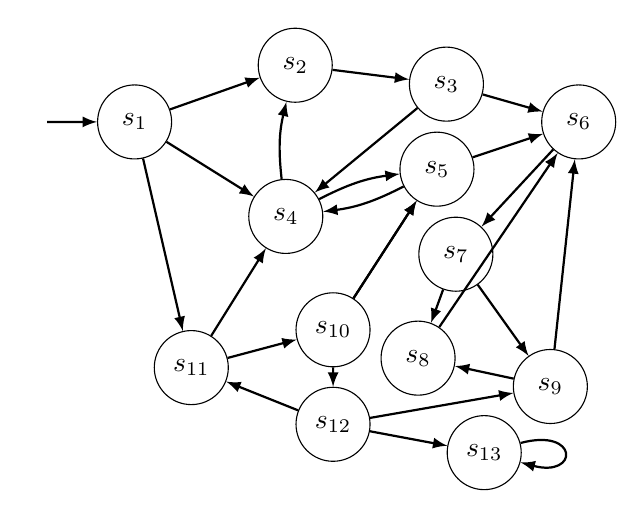
\begin{tikzpicture} [scale=1.2, every initial by arrow/.style={thick}]
		
		style/.mstate={minimum size=2}
			
%		\path
%		(\basex+.3,		\basey) 		node[mstate,initial,initial text=,initial distance=15pt] (s1) 	{$\state_1$} 
%		(\basex+2,		\basey+1.6) 		node[mstate] (s2) 	{$\state_2$} 
%		(\basex+3.6,	\basey+1.4) 	node[mstate] (s3) 	{$\state_3$} 
%		(\basex+1.9,		\basey+0) 		node[mstate] (s4) {$\state_4$} 
%		(\basex+3.5,		\basey+0.5)		node[mstate] (s5) 	{$\state_5$} 
%		(\basex+3.7,		\basey-.4) 		node[mstate] (s6) 	{$\state_6$} 
%		(\basex+5,	\basey) 		node[mstate] (s7) 	{$\state_7$} 
%		(\basex+2.4,	\basey-1.2) 	node[mstate] (s8) 	{$\state_8$} 
%		(\basex+3.3,		\basey-1.5) 	node[mstate] (s9) 	{$\state_9$} 
%		(\basex+.9,		\basey-1.6) 	node[mstate] (s10) 	{$\state_{10}$} 
%		(\basex+4.7,		\basey-1.8) 		node[mstate] (s11) 	{$\state_{11}$} 
%		(\basex+2.4,	\basey-2.2)		node[mstate] (s12) 	{$\state_{12}$} 
%		(\basex+4,		\basey-2.5) 		node[mstate] (s13) 	{$\state_{13}$} 
%		
%		;
		\path
		(\basex+.3,		\basey) 		node[mstate,initial,initial text=,initial distance=15pt] (s1) 	{$\state_1$} 
		(\basex+2,		\basey+1.6) 		node[mstate] (s2) 	{$\state_2$} 
		(\basex+3.6,	\basey+1.4) 	node[mstate] (s3) 	{$\state_3$} 
		(\basex+1.9,		\basey+0) 		node[mstate] (s4) {$\state_4$} 
		(\basex+3.5,		\basey+0.5)		node[mstate] (s5) 	{$\state_5$} 
		(\basex+3.7,		\basey-.4) 		node[mstate] (s6) 	{$\state_7$} 
		(\basex+5,	\basey) 		node[mstate] (s7) 	{$\state_6$} 
		(\basex+2.4,	\basey-1.2) 	node[mstate] (s8) 	{$\state_{10}$} 
		(\basex+3.3,		\basey-1.5) 	node[mstate] (s9) 	{$\state_8$} 
		(\basex+.9,		\basey-1.6) 	node[mstate] (s10) 	{$\state_{11}$} 
		(\basex+4.7,		\basey-1.8) 		node[mstate] (s11) 	{$\state_{9}$} 
		(\basex+2.4,	\basey-2.2)		node[mstate] (s12) 	{$\state_{12}$} 
		(\basex+4,		\basey-2.5) 		node[mstate] (s13) 	{$\state_{13}$} 
		
		;
		
		\path [trans] (s1) edge (s2);
		\path [trans] (s1) edge (s4);
		\path [trans] (s1) edge (s10);
		\path [trans] (s2) edge (s3);
		\path [trans] (s3) edge (s4);
		\path [trans] (s3) edge (s7);
		\path [bendtrans] (s4) edge (s2);
		\path [bendtrans] (s4) edge (s5);
		\path [bendtrans] (s5) edge (s4);
		\path [trans] (s5) edge (s7);
		\path [trans] (s6) edge (s9);
		\path [trans] (s6) edge (s11);
		\path [trans] (s7) edge (s6);
		\path [trans] (s8) edge (s5);
		\path [trans] (s8) edge (s12);
		\path [trans] (s8) edge (s5);
		\path [trans] (s9) edge (s7);
		\path [trans] (s10) edge (s4);
		\path [trans] (s10) edge (s8);
		\path [trans] (s11) edge (s7);
		\path [trans] (s11) edge (s9);
		\path [trans] (s12) edge (s10);
		\path [trans] (s12) edge (s11);
		\path [trans] (s12) edge (s13);

		\path [trans] (s13) edge [loop right] (s13);
 		
%		\path [trans, bend right=25] 		(sbot) 	edge node [midway,above left]		{\actionc} 		(s4);
%		\path [trans] 		(sbot) 	edge node [midway,right]			{\actionb} 		(s3);
%		\path [trans, bend right=25] 		(sbot) 	edge node [midway,left]				{\action} 		(s3);
%		\path [trans, bend left=25](sbot) 	edge node [midway,left]			{\actionb} 		(s5);
%		\path [trans, bend left=45] (sbot) 	edge node [midway,right]		{\actionc} 		(s5);
%		\path [trans,bend right=35] 	(s3) 	edge node [midway,right]	{\actionc} 		(sbot);
%		\path [trans] 	(s3) 	edge node [midway,above left]	{\action} 		(s4);
%		\path [trans] 	(s5) 	edge node [midway,above]	{\actionc} 		(s4);
%		
%		\path [trans] 		(sbot) 	edge [loop, in=15, out=50, looseness=6] node [midway,right] {\action,\actionb} 	(sbot);
%		\path [trans] 		(s3) 	edge [loop right] node [midway,below=4pt] {\actionb} 	(s3);
%		\path [trans] 		(s4) 	edge [loop below] node [midway,below] {\action} 	(s4);
%		\path [trans] 		(s6) 	edge [loop above] node [midway,above] {\actionc} 	(s6);
		
		
		%		midway, at start, near start, very near start, at end, near end, very near end
		
		
	\end{tikzpicture}
\end{document}
	\end{minipage}
	\begin{minipage}{.5\textwidth}
%		\hspace{5mm}
		\documentclass[tikz,preview]{standalone}
%\usepackage{prelude}

%%%%%%%%%%%%%%%%%%%%%%%%%%%%%%%%%%%% PACKAGES %%%%%%%%%%%%%%%%%%%%%%%%%%%%%%%%%%%%%%%%%%

\usepackage{inputenc,fontenc}
\usepackage[a4paper,margin=3cm]{geometry}
\usepackage[english]{babel}
%\usepackage[german]{babel}
%\usepackage[fixlanguage]{babelbib}


\usepackage{bbold}
\usepackage{amsthm}
\usepackage{amsmath}
\usepackage{amssymb} % doteqdot
\usepackage[dvipsnames]{xcolor}
\usepackage{standalone}
\usepackage{tikz}[mode=buildnew]
\usepackage{cite}
\usepackage{xspace}
\usepackage{relsize}
\usepackage{mathtools} % mathclap
%\usepackage{MnSymbol}
\usepackage{hyperref}
\usepackage{url}
\usepackage{listings} % for code
\usepackage[T1]{fontenc} %<
\hypersetup{
	colorlinks,
	citecolor=black,
	filecolor=black,
	linkcolor=black,
	urlcolor=black
}
\usepackage{pgfplots}
\pgfplotsset{compat=1.18}
%\usepackage{courier} %% Sets font for listing as Courier. But also for url and texttt!
\usepackage{listings, xcolor}
\usepackage{graphicx}
\usepackage{subcaption}

\usetikzlibrary{calc}
%\usepackage{xparse} % \newDocumentCommand for multiple optional arguments
%\usepackage{titlecaps}



%%%%%%%%%%%%%%%%%%%%%%%%%%%%%%%%%%%% THEOREMSTYLES %%%%%%%%%%%%%%%%%%%%%%%%%%%%%%%%%%

\theoremstyle{definition}
\newtheorem{definition}{Definition}[section]
\newtheorem{exmp}{Beispiel}[section]
%\AfterEndEnvironment{definition}{\noindent\ignorespaces}

\theoremstyle{theorem}
\newtheorem{theorem}{Satz}[section]
\newtheorem{proposition}{Proposition}[section]
%\AfterEndEnvironment{theorem}{\noindent\ignorespaces}

\theoremstyle{korollary}
\newtheorem{korollary}{Korollar}[section]
%\AfterEndEnvironment{korollary}{\noindent\ignorespaces}


\tikzset{
	mstate/.style={draw, circle, minimum size=.94cm}, 
	gstate/.style={draw, rectangle, minimum size=.8cm},
	varstate/.style={draw,rectangle, rounded corners, minimum size=1}, 
	trans/.style={draw, ->, thick},
	bendtrans/.style={draw, ->, thick, bend left=10},
	bendtransr/.style={draw, ->, thick, bend right=10},
	init/.style={initial, initial distance=6pt, initial text=},
	every loop/.style={min distance=5pt, looseness=8},
	>=latex
}
\usetikzlibrary{automata,positioning}

%auto shift/.style={auto=right,->,
%	to path={ let \p1=(\tikztostart),\p2=(\tikztotarget),
%		\n1={atan2(\y2-\y1,\x2-\x1)},\n2={\n1+180}
%		in ($(\tikztostart.{\n1})!1mm!270:(\tikztotarget.{\n2})$) -- 
%		($(\tikztotarget.{\n2})!1mm!90:(\tikztostart.{\n1})$) \tikztonodes}},

%%%%%%%%%%%%%%%%%%%%%%%%%%%%%%%%%%% MY MACROS %%%%%%%%%%%%%%%%%%%%%%%%%%%%%%%%%%%%%%%%%
%formatting
\newcommand{\comment}[2]{{\color{#1}#2}}
\newcommand{\redcomment}[1]{{\color{red}#1}}
\newcommand{\purpcomment}[1]{{\color{pink}#1}}
\newcommand{\bluecomment}[1]{{\color{blue}#1}}
\newcommand{\mt}[1]{\ensuremath{{#1}}\xspace}
\newcommand{\mynewcommand}[2]{\newcommand{#1}{\mt{#2}}} %% currently not used becaue of ide highlighting
\newcommand{\arr}{\mt{\to}}

%model checking terms
\newcommand{\mimicrel}{\mt{\mathcal{R}}}
\newcommand{\bisimeq}{\mt{\;\!\sim\;\!}}
\newcommand{\simorder}{\mt{\;\!\preceq\;\!}}
\newcommand{\simequiv}{\mt{\;\!\simeq\;\!}} %command already defined
\newcommand{\relts}{\mt{\;\!\bullet_{_{\tiny{TS}}}\;\!}}
\newcommand{\rel}{\mt{\;\!\bullet\;\!}}

%own names
\newcommand{\nm}[1]{#1\xspace}
\newcommand{\mdpN}{\nm{MDP}}
\newcommand{\mdpsN}{\nm{MDPs}}
\newcommand{\viewN}{\nm{view}}
\newcommand{\viewNC}{\nm{View}}
\newcommand{\viewsN}{\nm{views}}
\newcommand{\viewsNC}{\nm{Views}}
\newcommand{\grpfctsubN}{\nm{detached grouping function}}
\newcommand{\grpfctsubNC}{\nm{detached grouping function}}
\newcommand{\grpfctsubNCC}{\nm{Detached Grouping Function}}
\newcommand{\grpfctN}{\nm{grouping function}}
\newcommand{\grpfctNC}{\nm{Grouping function}}
\newcommand{\grpfctNCC}{\nm{Grouping Function}}
\newcommand{\grpfctsN}{\nm{grouping functions}}
\newcommand{\grpfctsNC}{\nm{Grouping functions}}
\newcommand{\grpfctsNCC}{\nm{Grouping Functions}}
\newcommand{\stmimicN}{\nm{state-mimic}}
\newcommand{\stmimicsN}{\nm{state-mimics}}
\newcommand{\stmimickingN}{\nm{state-mimicking}}
\newcommand{\stmimickedN}{\nm{state-mimicked}}
%\newcommand{\chosenphtypeNCC}{\nm{Transition System}}
%\newcommand{\chgphNC}{\nm{Transition system}}
%\newcommand{\chgphN}{\nm{transition system}}
%\newcommand{\chgphsNCC}{\nm{Transition Systems}}
%\newcommand{\chgphsNC}{\nm{Transition systems}}
%\newcommand{\chgphsN}{\nm{transition systems}}
\newcommand{\chgphNCC}{\nm{MDP}}
\newcommand{\chgphNC}{\nm{MDP}}
\newcommand{\chgphN}{\nm{MDP}}
\newcommand{\achgphN}{\nm{an MDP}}
\newcommand{\chgphsNCC}{\nm{MDPs}}
\newcommand{\chgphsNC}{\nm{MDPs}}
\newcommand{\chgphsN}{\nm{MDPs}}
\newcommand{\parllcompN}{\nm{parallel composition}}
\newcommand{\parllcompNC}{\nm{Parallel composition}}
\newcommand{\parllcompNCC}{\nm{Parallel Composition}}
\newcommand{\parllcompsN}{\nm{parallel compositions}}
\newcommand{\parllcompsNC}{\nm{Parallel compositions}}
\newcommand{\parllcompsNCC}{\nm{Parallel Compositions}}
\newcommand{\sccN}{\nm{SCC}}
\newcommand{\sccsN}{\nm{SCCs}}
\newcommand{\bsccN}{\nm{BSCC}}
\newcommand{\bsccsN}{\nm{BSCCs}}
\newcommand{\jgrapht}{\nm{jGraphtT}}

\newcommand{\outactident}{\nm{OutActionsIdent}}

%names
\newcommand{\iffN}{\nm{if and only if}}
\newcommand{\tsN}{\nm{TS}}

%% outactions identical
\newcommand{\outactidentstrong}{\nm{strong}}
\newcommand{\outactidentweak}{\nm{weak}}

% CORE DEFINITIONS
\newcommand{\grpfct}[1][\viewppty]{\mt{F_{#1}}}
\newcommand{\grpfctsub}[1][\viewppty]{\mt{\tilde{F}_{#1}}}
%\newcommand{\grpfctimg}[1]{\mt{{\grpfct}[{#1}]}}
%\newcommand{\fctimg}[2]{\mt{{#1}[{#2}]}}
\newcommand{\eqrelview}{\mt{R}}
\newcommand{\eqclassv}[1][\state]{\mt{\eqclass{#1}{\eqrelview}}}
\newcommand{\eqclasssetv}[1][\states]{\mt{{#1}/\eqrelview}} %OLD: \bigcup_{\state \in \states} \eqclassv
\newcommand{\viewid}{\mt{\mdp}}
\newcommand{\view}[1][\viewppty]{\mt{\viewid_{#1}}}
\newcommand{\imggrp}{\mt{\arbset}}
\newcommand{\imggrpsub}{\mt{X}}
\newcommand{\viewppty}{\mt{\theta}}
\newcommand{\pll}{\mt{\;\!\pllpure\;\!}}
\newcommand{\pllrev}{\mt{\pllpure^{-1}}}
\newcommand{\pllpure}{\mt{||}}
\newcommand{\compselectset}{\mt{Z}}
\newcommand{\compselectpure}{\mt{\pllpure_\compselectset}}
\newcommand{\compselect}{\mt{\;\pllpure_\compselectset\;}}
\newcommand{\remstates}{\mt{\bigcup_{\state \in \states \setminus \states_1}\{\{\state\}\}}}
\newcommand{\nogroupstates}[1][\states_2]{\mt{\bigcup_{\state \in \states \setminus {#1}}\{\{\state\}\}}}
\newcommand{\remelem}{\mt{\bullet}}
\newcommand{\nogroupset}{\mt{\xi}}
\newcommand{\remset}{\mt{\{\remelem\}}}
\newcommand{\gfctpll}{\mt{\grpfct[\pll]}}
\newcommand{\group}{\mt{\top}}
\newcommand{\imggrpbinview}{\mt{\{\remelem, \notppty\}}}
\newcommand{\viewappset}{\mt{\tilde{\states}}}
\newcommand{\hasppty}{\mt{\top}}
\newcommand{\notppty}{\mt{\bot}}
\newcommand{\disregardelem}{\mt{\Delta}}
\newcommand{\disregardelements}{\mt{{\disregardelem_1, \dots, \disregardelem_n}}}



%\newcommand{\mdp}{def}\mdp
%\newcommand{\mdpdef}



% EXAMPLE VIEWS
\newcommand{\pptyatomicprops}{\mt{\atomicprops}}
\newcommand{\pptyinitstates}{\mt{\initstates}}
\newcommand{\pptyinactsetsize}{\mt{|\inacts(\state)|}}
\newcommand{\pptyhasoutact}{\mt{\exists\outact}}
\newcommand{\pptyminoutact}[2]{\mt{#1\leq#2}}
\newcommand{\pptymaxoutact}[2]{\mt{#2\leq#1}}
\newcommand{\pptyspanoutact}[3]{\mt{#1\leq#2\leq#3}}
\newcommand{\pptyoutactsetsize}{\mt{|\outacts(\state)|}}
\newcommand{\pptyoutactsingle}{\mt{|\outacts(\state)|_1}}
\newcommand{\pptystrongoutactident}{\mt{\outacts(\state)_=}}
\newcommand{\pptyweakoutactident}{\mt{\outacts(\state)_\approx}}
\newcommand{\pptyhasinact}{\mt{\exists\inact}}
\newcommand{\pptymininact}[2]{\mt{#1\leq#2}}
\newcommand{\pptymaxinact}[2]{\mt{#2\leq#1}}
\newcommand{\pptyspaninact}[3]{\mt{#1\leq#2\leq#3}}
\newcommand{\pptyinactsingle}{\mt{|\inacts(\state)|_1}}
\newcommand{\pptystronginactident}{\mt{\inacts(\state)_=}}
\newcommand{\pptyweakinactident}{\mt{\inacts(\state)_\approx}}
\newcommand{\pptyparamvalueseq}{\mt{\var = \varval}}
\newcommand{\pptyparamvaluesneq}{\mt{\var \neq \varval}}
\newcommand{\pptyparamdnf}{\mt{VarDNF}}
\newcommand{\pptyparamcnf}{\mt{VarCNF}}
\newcommand{\pptyparamvalueseqopt}{\mt{\var = \varval}}
\newcommand{\pptyparamvalident}{\mt{Var:\varval}}
\newcommand{\pptydistance}{\mt{\distpath}}
\newcommand{\pptydistancerev}{\mt{\distpathrev}}
\newcommand{\pptydistancebi}{\mt{\distpathbi}}
\newcommand{\pptyhascycle}{\mt{\exists\cycle}}
\newcommand{\pptyexactactcycle}{\mt{\{\cycle_{\action,n}\}}}
\newcommand{\pptycycleset}{\mt{\cup{\{\state\}_\cycle}}}
\newcommand{\pptyexactcycle}{\mt{\{\cycle_n\}}}
\newcommand{\pptyscc}{\mt{scc}}
\newcommand{\pptybscc}{\mt{bscc}}
\newcommand{\pptyprop}{\mt{\redcomment{?}}}
\newcommand{\pptyident}{id}


\newcommand{\gfctatomicprops}{\mt{\grpfct[\pptyatomicprops]}}
\newcommand{\gfctinitstates}{\mt{\grpfct[\pptyinitstates]^\hasppty}}
\newcommand{\gfcthasoutaction}{\mt{\grpfct[\pptyhasoutact]^\hasppty}}
\newcommand{\gfctminoutaction}{\mt{\grpfct[\pptyminoutact{\numoutact}{\outact}]^\hasppty}}
\newcommand{\gfctmaxoutaction}{\mt{\grpfct[\pptymaxoutact{\numoutact}{\outact}]^\hasppty}}
\newcommand{\gfctspanoutaction}{\mt{\grpfct[\pptyspanoutact{\numoutactb}{\outact}{\numoutact}]^\hasppty}}
\newcommand{\gfctoutactsetsize}{\mt{\grpfct[\pptyoutactsetsize]}}
\newcommand{\gfctoutactsingle}{\mt{\grpfct[\pptyoutactsingle]^\notppty}}
\newcommand{\gfctstrongoutactident}{\mt{\grpfct[\pptystrongoutactident]}}
\newcommand{\gfctweakoutactident}{\mt{\grpfct[\pptyweakoutactident]}}
\newcommand{\gfcthasinaction}{\mt{\grpfct[\pptyhasinact]^\hasppty}}
\newcommand{\gfctmininaction}{\mt{\grpfct[\pptymininact{\numinact}{\inact}]^\hasppty}}
\newcommand{\gfctmaxinaction}{\mt{\grpfct[\pptymaxinact{\numinact}{\inact}]^\hasppty}}
\newcommand{\gfctspaninaction}{\mt{\grpfct[\pptyspaninact{\numinactb}{\inact}{\numinact}]^\hasppty}}
\newcommand{\gfctinactsetsize}{\mt{\grpfct[\pptyinactsetsize]}}
\newcommand{\gfctinactsingle}{\mt{\grpfct[\pptyinactsingle]^\notppty}}
\newcommand{\gfctstronginactident}{\mt{\grpfct[\pptystronginactident]}}
\newcommand{\gfctweakinactident}{\mt{\grpfct[\pptyweakinactident]}}
\newcommand{\gfctparamvalueseq}{\mt{\grpfct[\pptyparamvalueseq]^\hasppty}}
\newcommand{\gfctparamvaluesneq}{\mt{\grpfct[\pptyparamvaluesneq]^\hasppty}}
\newcommand{\gfctparamdnf}{\mt{\grpfct[\pptyparamdnf]^\hasppty}}
\newcommand{\gfctparamcnf}{\mt{\grpfct[\pptyparamcnf]^\hasppty}}
\newcommand{\gfctparamvalueseqopt}{\mt{\pptyparamvalueseqopt}}
\newcommand{\gfctparamvalident}{\mt{\grpfct[\pptyparamvalident]}}
\newcommand{\gfctdistance}{\mt{\grpfct[\pptydistance]}}
\newcommand{\gfctdistancerev}{\mt{\grpfct[\pptydistancerev]}}
\newcommand{\gfctdistancebi}{\mt{\grpfct[\pptydistancebi]}}
\newcommand{\gfcthascycle}{\mt{\grpfct[\pptyhascycle]}}
\newcommand{\gfctexactcycle}{\mt{\grpfct[\pptyexactcycle]}}
\newcommand{\gfctcycleset}{\mt{\grpfct[\pptycycleset]}}
\newcommand{\gfctexactactcycle}{\mt{\grpfct[\pptyexactactcycle]}}
\newcommand{\gfctscc}{\mt{\grpfct[\pptyscc]}}
\newcommand{\gfctbscc}{\mt{\grpfct[\pptybscc]}}
\newcommand{\gfctprop}{\mt{\grpfct[\pptyprop]}}
\newcommand{\gfctident}{\mt{\grpfct[\pptyident]}}

\newcommand{\gfctsubatomicprops}{\mt{\grpfctsub[\pptyatomicprops]}}
\newcommand{\gfctsubinitstates}{\mt{\grpfctsub[\pptyinitstates]^\hasppty}}
\newcommand{\gfctsubhasoutaction}{\mt{\grpfctsub[\pptyhasoutact]^\hasppty}}
\newcommand{\gfctsubminoutaction}{\mt{\grpfctsub[\pptyminoutact{\numoutact}{\outact}]^\hasppty}}
\newcommand{\gfctsubmaxoutaction}{\mt{\grpfctsub[\pptymaxoutact{\numoutact}{\outact}]^\hasppty}}
\newcommand{\gfctsubspanoutaction}{\mt{\grpfctsub[\pptyspanoutact{\numoutactb}{\outact}{\numoutact}]^\hasppty}}
\newcommand{\gfctsuboutactsetsize}{\mt{\grpfctsub[\pptyoutactsetsize]}}
\newcommand{\gfctsuboutactsingle}{\mt{\grpfctsub[\pptyoutactsingle]^\notppty}}
\newcommand{\gfctsubstrongoutactident}{\mt{\grpfctsub[\pptystrongoutactident]^\hasppty}}
\newcommand{\gfctsubweakoutactident}{\mt{\grpfctsub[\pptyweakoutactident]^\hasppty}}
\newcommand{\gfctsubhasinaction}{\mt{\grpfctsub[\pptyhasinact]}}
\newcommand{\gfctsubmininaction}{\mt{\grpfctsub[\pptymininact{\numinact}{\inact}]}}
\newcommand{\gfctsubmaxinaction}{\mt{\grpfctsub[\pptymaxinact{\numinact}{\inact}]}}
\newcommand{\gfctsubspaninaction}{\mt{\grpfctsub[\pptyspaninact{\numinactb}{\inact}{\numinact}]}}
\newcommand{\gfctsubinactsetsize}{\mt{\grpfctsub[\pptyinactsetsize]^\hasppty}}
\newcommand{\gfctsubinactsingle}{\mt{\grpfctsub[\pptyinactsingle]^\notppty}}
\newcommand{\gfctsubstronginactident}{\mt{\grpfctsub[\pptystronginactident]}}
\newcommand{\gfctsubweakinactident}{\mt{\grpfctsub[\pptyweakinactident]}}
\newcommand{\gfctsubparamvalueseq}{\mt{\grpfctsub[\pptyparamvalueseq]^\hasppty}}
\newcommand{\gfctsubparamvaluesneq}{\mt{\grpfctsub[\pptyparamvaluesneq]^\hasppty}}
\newcommand{\gfctsubparamdnf}{\mt{\grpfctsub[\pptyparamdnf]^\hasppty}}
\newcommand{\gfctsubparamcnf}{\mt{\grpfctsub[\pptyparamcnf]^\hasppty}}
\newcommand{\gfctsubparamvalueseqopt}{\mt{\pptyparamvalueseqopt}}
\newcommand{\gfctsubparamvalident}{\mt{\grpfctsub[\pptyparamvalident]}}
\newcommand{\gfctsubdistance}{\mt{\grpfctsub[\pptydistance]}}
\newcommand{\gfctsubdistancerev}{\mt{\grpfctsub[\pptydistancerev]}}
\newcommand{\gfctsubdistancebi}{\mt{\grpfctsub[\pptydistancebi]}}
\newcommand{\gfctsubhascycle}{\mt{\grpfctsub[\pptyhascycle]^\hasppty}}
\newcommand{\gfctsubexactcycle}{\mt{\grpfctsub[\pptyexactcycle]}}
\newcommand{\gfctsubcycleset}{\mt{\grpfctsub[\pptycycleset]}}
\newcommand{\gfctsubexactactcycle}{\mt{\grpfctsub[\pptyexactactcycle]}}
\newcommand{\gfctsubscc}{\mt{\grpfctsub[\pptyscc]}}
\newcommand{\gfctsubbscc}{\mt{\grpfctsub[\pptybscc]}}
\newcommand{\gfctsubprop}{\mt{\grpfctsub[\pptyprop]}}
\newcommand{\gfctsubident}{\mt{\grpfctsub[\pptyident]}}


\newcommand{\viewatomicprops}{\mt{\view[\pptyatomicprops]}}
\newcommand{\viewinitstates}{\mt{\view[\pptyinitstates]^\hasppty}}
\newcommand{\viewhasoutaction}{\mt{\view[\pptyhasoutact]^\hasppty}}
\newcommand{\viewminoutaction}{\mt{\view[\pptyminoutact{\numoutact}{\outact}]^\hasppty}}
\newcommand{\viewmaxoutaction}{\mt{\view[\pptymaxoutact{\numoutact}{\outact}]^\hasppty}}
\newcommand{\viewspanoutaction}{\mt{\view[\pptyspanoutact{\numoutactb}{\outact}{\numoutact}]^\hasppty}}
\newcommand{\viewoutactsetsize}{\mt{\view[\pptyoutactsetsize]}}
\newcommand{\viewoutactsingle}{\mt{\view[\pptyoutactsingle]^\notppty}}
\newcommand{\viewstrongoutactident}{\mt{\view[\pptystrongoutactident]}}
\newcommand{\viewweakoutactident}{\mt{\view[\pptyweakoutactident]}}
\newcommand{\viewhasinaction}{\mt{\view[\pptyhasinact]^\hasppty}}
\newcommand{\viewmininaction}{\mt{\view[\pptymininact{\numinact}{\inact}]^\hasppty}}
\newcommand{\viewmaxinaction}{\mt{\view[\pptymaxinact{\numinact}{\inact}]^\hasppty}}
\newcommand{\viewspaninaction}{\mt{\view[\pptyspaninact{\numinactb}{\inact}{\numinact}]^\hasppty}}
\newcommand{\viewinactsetsize}{\mt{\view[\pptyinactsetsize]}}
\newcommand{\viewinactsingle}{\mt{\view[\pptyinactsingle]^\notppty}}
\newcommand{\viewstronginactident}{\mt{\view[\pptystronginactident]}}
\newcommand{\viewweakinactident}{\mt{\view[\pptyweakinactident]}}
\newcommand{\viewparamvalueseq}{\mt{\view[\pptyparamvalueseq]}}
\newcommand{\viewparamvaluesneq}{\mt{\view[\pptyparamvaluesneq]}}
\newcommand{\viewparamdnf}{\mt{\view[\pptyparamdnf]^\hasppty}}
\newcommand{\viewparamcnf}{\mt{\view[\pptyparamcnf]^\hasppty}}
\newcommand{\viewparamvalueseqopt}{\mt{\pptyparamvalueseqopt}}
\newcommand{\viewparamvalident}{\mt{\view[\pptyparamvalident]}}
\newcommand{\viewdistance}{\mt{\view[\pptydistance]}}
\newcommand{\viewdistancerev}{\mt{\view[\pptydistancerev]}}
\newcommand{\viewdistancebi}{\mt{\view[\pptydistancebi]}}
\newcommand{\viewhascycle}{\mt{\view[\pptyhascycle]}}
\newcommand{\viewexactcycle}{\mt{\view[\pptyexactcycle]}}
\newcommand{\viewcycleset}{\mt{\view[\pptycycleset]}}
\newcommand{\viewexactactcycle}{\mt{\view[\pptyexactactcycle]}}
\newcommand{\viewscc}{\mt{\view[\pptyscc]}}
\newcommand{\viewbscc}{\mt{\view[\pptybscc]}}
\newcommand{\viewprop}{\mt{\view[\pptyprop]}}
\newcommand{\viewident}{\mt{\view[\pptyident]}}

%\newcommand{\viewatomicprops}{\mt{\view[\atomicprops]}}
%\newcommand{\viewinitstates}{\mt{\view[\initstates]}}
%\newcommand{\viewhasoutaction}{\mt{\view[\pptyhasoutact]}}
%\newcommand{\viewminoutaction}{\mt{\view[\pptyminoutact{\numoutact}{\outact}]}}
%\newcommand{\viewmaxoutaction}{\mt{\view[\pptymaxoutact{\numoutact}{\outact}]}}
%\newcommand{\viewspanoutaction}{\mt{\view[\pptyspanoutact{\numoutactb}{\outact}{\numoutact}]}}
%\newcommand{\viewoutactsetsize}{\mt{\view[\pptyoutactsetsize]}}
%\newcommand{\viewoutactsingle}{\mt{\view[\pptyoutactsingle]}}
%\newcommand{\viewstrongoutactident}{\mt{\view[\outacts(\state)_=]}}
%\newcommand{\viewweakoutactident}{\mt{\view[\outacts(\state)_\approx]}}
%\newcommand{\viewhasinaction}{\mt{\view[\pptyhasinact]}}
%\newcommand{\viewmininaction}{\mt{\view[\pptymininact{\numinact}{\inact}]}}
%\newcommand{\viewmaxinaction}{\mt{\view[\pptymaxinact{\numinact}{\inact}]}}
%\newcommand{\viewspaninaction}{\mt{\view[\pptyspaninact{\numinactb}{\inact}{\numinact}]}}
%\newcommand{\viewinactsetsize}{\mt{\view[\pptyinactsetsize]}}
%\newcommand{\viewinactsingle}{\mt{\view[\pptyinactsingle]}}
%\newcommand{\viewstronginactident}{\mt{\view[\inacts(\state)_=]}}
%\newcommand{\viewweakinactident}{\mt{\view[\inacts(\state)_\approx]}}
%\newcommand{\viewparamvalueseq}{\mt{\view[\var = \varval]}}
%\newcommand{\viewparamvaluesneq}{\mt{\view[\var \neq \varval]}}
%\newcommand{\viewparamdnf}{\mt{\view[VarDNF]}}
%\newcommand{\viewparamcnf}{\mt{\view[VarCNF]}}
%\newcommand{\viewparamvalident}{\mt{\view[\pptyparamvalident]}}
%\newcommand{\viewdistance}{\mt{\view[\pptydistance]}}
%\newcommand{\viewhascycle}{\mt{\view[\exists\cycle]}}
%\newcommand{\viewexactcycle}{\mt{\view[\pptyexactcycle]}}
%\newcommand{\viewcycleset}{\mt{\view[\pptycycleset]}}
%\newcommand{\viewexactactcycle}{\mt{\view[\pptyexactactcycle]}}
%\newcommand{\viewscc}{\mt{\view[scc]}}
%\newcommand{\viewbscc}{\mt{\view[bscc]}}

%actions
\newcommand{\numoutact}{\mt{n}}
\newcommand{\numoutactb}{\mt{m}}
\newcommand{\numinact}{\mt{n}}
\newcommand{\numinactb}{\mt{m}}

\newcommand{\predmaxoutact}[1][\numoutact]{\mt{Q_{\outact\leq#1}(\state,\state_1, \dots, \state_{#1+1})}}
\newcommand{\predminoutact}[1][\numoutact]{\mt{Q_{#1\leq\outact}(\state,\state_1, \dots, \state_{#1})}}
\newcommand{\formoutact}[1][\state]{\mt{C_{#1,\outact}}}
\newcommand{\predmaxinact}[1][\numinact]{\mt{Q_{\inact\leq#1}(\state,\state_1, \dots, \state_{#1+1})}}
\newcommand{\predmininact}[1][\numinact]{\mt{Q_{#1\leq\inact}(\state,\state_1, \dots, \state_{#1})}}

\newcommand{\outact}[1][\action]{\mt{\overrightarrow{#1}}}
\newcommand{\outacts}{\mt{\overrightarrow{\actions}}}
\newcommand{\inact}{\mt{\overleftarrow{\action}}}
\newcommand{\inacts}[1][\action]{\mt{\overleftarrow{#1}}}

%%Parameters
\newcommand{\vars}[1][\mdp]{\mt{V\!ar_{#1}}}
\newcommand{\var}{\mt{x}}
\newcommand{\varstate}[1][]{\mt{\var_{\state#1}}}
\newcommand{\varval}{\mt{a}}
\newcommand{\vareval}[1][\mdp]{\mt{V\!arEval_{#1}}}
\newcommand{\varevalimg}[1][\mdp]{\mt{\vareval[#1][\states,\vars]}}
\newcommand{\varevalimgset}{\mt{\arbset}}
\newcommand{\someparam}{\mt{\tilde{x}}}
\newcommand{\eqorneq}{\mt{\;\doteqdot\;}}
\newcommand{\varstyle}[2]{\mt{\langle#1,#2\rangle}}




%\makeatletter
%\newcommand{\overleftrightsmallarrow}{\mathpalette{\overarrowsmall@\leftrightarrowfill@}}
%\newcommand{\overrightsmallarrow}{\mathpalette{\overarrowsmall@\rightarrowfill@}}
%\newcommand{\overleftsmallarrow}{\mathpalette{\overarrowsmall@\leftarrowfill@}}
%\newcommand{\overarrowsmall@}[3]{%
%	\vbox{%
%		\ialign{%
%			##\crcr
%			#1{\smaller@style{#2}}\crcr
%			\noalign{\nointerlineskip}%
%			$\m@th\hfil#2#3\hfil$\crcr
%		}%
%	}%
%}
%\def\smaller@style#1{%
%	\ifx#1\displaystyle\scriptstyle\else
%	\ifx#1\textstyle\scriptstyle\else
%	\scriptscriptstyle
%	\fi
%	\fi
%}
%\makeatother
%\newcommand{\te}[1]{\overleftrightsmallarrow{#1}}

% Distance
\newcommand{\fctdist}{\mt{distance}}
\newcommand{\fctdistdefault}{\mt{\fctdist(\chgph, \smstates, \grandist)}}
\newcommand{\distval}{\mt{d}}
\newcommand{\grandist}{\mt{n}}
\let\path\oldpath
\newcommand{\path}{\mt{P}}
\newcommand{\pathbi}{\mt{\bar{\path}}}
\newcommand{\pathsecfull}{\mt{(\state_0, \action_0, \state_1, \action_1, \dots, \action_{n}, \state_{n+1})}}
\newcommand{\lenpath}{\mt{len}}
\newcommand{\pfirst}{\mt{first}}
\newcommand{\plast}{\mt{last}}
\newcommand{\pathset}{\mt{\path_\chgph}}
\newcommand{\pathbiset}{\mt{\pathbi_\chgph}}
\newcommand{\distpath}{\mt{\overrightarrow{dist}}}
\newcommand{\distpathrev}{\mt{\overleftarrow{dist}}}
\newcommand{\distpathbi}{\mt{\overline{dist}}}
%Cycles
\newcommand{\cyclesecfull}{\mt{(\state_0, \action_0, \state_1, \action_1, \dots, \action_{n-1}, \state_0)}}
\newcommand{\fctfindcycles}{\mt{findCycles}}
\newcommand{\cycle}{\mt{C}}
\newcommand{\cycleset}{\mt{\cycle_{\mdp, n}}}
\newcommand{\lencycle}{\mt{len}}
% strongly connected components
\newcommand{\scc}{\mt{T}}
\newcommand{\setscc}{\mt{SCC_{\chgph,n}}}
\newcommand{\setbscc}{\mt{BSCC_{\chgph,n}}}

% properties
\newcommand{\propfct}{\mt{f}}

% all Systems
\newcommand{\chgph}{\mt{\mdp}}
\newcommand{\chgphtuple}{\mt{\mdptuple}}
\newcommand{\chgphtupledist}{\mt{\mdptupledist}}

\newcommand{\states}{\mt{S}}
\newcommand{\actions}{\mt{Act}}
\newcommand{\atomicprops}{\mt{AP}}
\newcommand{\labelingfct}{\mt{L}}
\newcommand{\init}{\mt{\initdistrib}} % use MDP % refers to the underlying set
\newcommand{\trans}{\mt{\probtfunc}} % use MDP % refers to the underlying set
\newcommand{\smstates}{\mt{\tilde{\states}}}


\newcommand{\state}{\mt{s}}
\newcommand{\action}{\mt{\alpha}}
\newcommand{\actionb}{\mt{\beta}}
\newcommand{\actionc}{\mt{\gamma}}
\newcommand{\smstate}{\mt{\tilde{\state}}}



% transition sysstems
\newcommand{\ts}{\mt{TS}}
\newcommand{\transitionrel}{\mt{\longrightarrow}}
\newcommand{\initstates}{\mt{I}}
\newcommand{\transitionsystem}{\mt
	{(\states, \actions, \transitionrel, \initstates, \atomicprops, \labelingfct)}
}
\newcommand{\tstupledist}{\mt{(\states', \actions',\transitionrel', \initstates', \labelingfct')}}


%Markov chains and MDP
\newcommand{\mdp}{\mt{\autm}}
\newcommand{\mdptuple}{\mt{(\states, \actions, \probtfunc, \initdistrib, \atomicprops, \labelingfct)}}
\newcommand{\mdptupledist}{\mt{(\states', \actions', \probtfunc', \initdistrib', \atomicprops', \labelingfct')}}
\newcommand{\autm}{\mt{\mathcal{M}}}
\newcommand{\probtfunc}{\mt{\textbf{P}}}
\newcommand{\initdistrib}{\mt{\iota_{init}}}


%maths
\newcommand{\powerset}[1]{\mt{\mathcal{P}(#1)}}
\newcommand{\eqclass}[2]{\mt{[#1]_{#2}}}%{\mt{#1 / #2}}
\newcommand{\impr}{\mt{\hspace{3mm}\Rightarrow\hspace{2mm}}}
\newcommand{\impl}{\mt{\hspace{3mm}\Leftarrow\hspace{2mm}}}
\newcommand{\natnums}{\mt{\mathbb{N}}} 
\newcommand{\realnums}{\mt{\mathbb{R}}}
\newcommand{\intmodn}[1][n]{\mt{\mathbb{Z}_{#1}}}
\newcommand{\arbset}{\mt{M}}
\newcommand{\bigsum}[2][]{\mt{\mathlarger{\sum}_{#2}^{#1}}}
\newcommand{\bbigsum}[2][]{\mt{\mathlarger{\mathlarger{\sum}}_{#2}^{#1}}}
\newcommand{\invimage}[2]{#1^{\mt{-1}(#2)}}
\newcommand{\img}{\mt{Img}}
\newcommand{\cond}{\mt{\,|\,}}

%tickz
%% \definecolor{darkred}{RGB}{196, 42, 42}

%implementation
\newcommand{\pmcvis}{\nm{PMC-Vis}}



\begin{document}
	\newcommand{\basex}{0}
	\newcommand{\basey}{0}
	\newcommand{\createstate}[3]{\node[draw, circle, minimum size=1cm] (#1) at (#2) {#3}}
	
	
	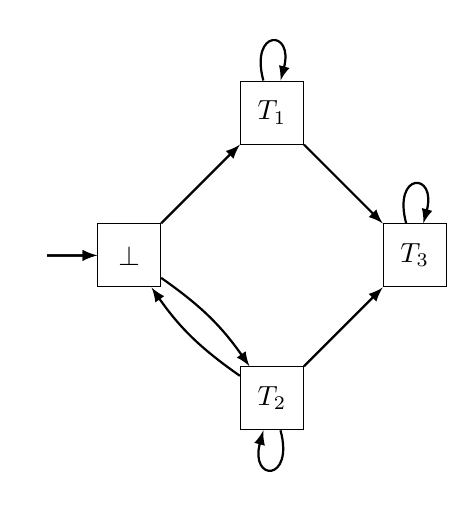
\begin{tikzpicture} [scale=3, every initial by arrow/.style={thick}]
		
		
		\path
		(\basex,		\basey) 		node[gstate,init, initial left] (sbot) 	{$\notppty$} 
		
		;
		
		\node[gstate, above right = of sbot] (t1) 	{$\scc_1$};
		\node[gstate, below right = of sbot] (t2) 	{$\scc_2$};
		\node[gstate, above right = of t2] 	 (t3) 	{$\scc_3$};
		
	
		\path [trans] 		(sbot) 	edge node [midway,above]	{} 		(t1);		
		\path [bendtrans] 	(sbot) 	edge node [midway,above]	{} 		(t2);		
		\path [trans] 		(t1) 	edge node [midway,above]	{} 		(t3);		
		\path [bendtrans] 	(t2) 	edge node [midway,above]	{} 		(sbot);		
		\path [trans] 		(t2) 	edge node [midway,above]	{} 		(t3);	
		
		\path [trans] (t1)	edge [loop above] (t1);
		\path [trans] (t2)	edge [loop below] (t1);
		\path [trans] (t3)	edge [loop above] (t3);
			
		
	\end{tikzpicture}
\end{document}
	\end{minipage}
		\caption{Simplified representations of \mdp (left) and the \viewN \viewscc on it (right)}
		\label{fig:sccMin2}  
\end{figure}

A special kind of strongly connected components is the the bottom strongly connected component.

\begin{definition}
	Let \scc be a \sccN. A \emph{bottom strongly connected component} (\bsccN) is a \sccN where it holds that: \redcomment{concurrent versions}
	\[
	\forall \state \in \scc : \forall (\state, \action, \state') \in \trans : \state' \in \scc
	\]
	\[
	\forall \state \in \scc : \bigsum{t \in \scc} \trans(\state, t) = 1
	\]
	That is from \scc there is no state reachable outside of \scc. The set of bottom strongly connected components of \chgph is denoted with \setbscc.
\end{definition}

\redcomment{These are of special relevance because..}

\begin{definition}
	Let $\chgph = \chgphtuple$ be \achgphN. The \viewN \viewbscc is defined by its \grpfctN $\gfctbscc : \states \to \imggrp$ with
	\[
	\state \mapsto \{\scc \in \setbscc \mid \state \in \scc, n \leq |\scc|\}
	\]
	and $\imggrp = \setbscc \cup \remset$.
\end{definition}

\begin{figure}[h]
	\begin{minipage}{.55\textwidth}
		\hspace{5mm}
		\documentclass[tikz,preview]{standalone}
%\usepackage{prelude}

%%%%%%%%%%%%%%%%%%%%%%%%%%%%%%%%%%%% PACKAGES %%%%%%%%%%%%%%%%%%%%%%%%%%%%%%%%%%%%%%%%%%

\usepackage{inputenc,fontenc}
\usepackage[a4paper,margin=3cm]{geometry}
\usepackage[english]{babel}
%\usepackage[german]{babel}
%\usepackage[fixlanguage]{babelbib}


\usepackage{bbold}
\usepackage{amsthm}
\usepackage{amsmath}
\usepackage{amssymb} % doteqdot
\usepackage[dvipsnames]{xcolor}
\usepackage{standalone}
\usepackage{tikz}[mode=buildnew]
\usepackage{cite}
\usepackage{xspace}
\usepackage{relsize}
\usepackage{mathtools} % mathclap
%\usepackage{MnSymbol}
\usepackage{hyperref}
\usepackage{url}
\usepackage{listings} % for code
\usepackage[T1]{fontenc} %<
\hypersetup{
	colorlinks,
	citecolor=black,
	filecolor=black,
	linkcolor=black,
	urlcolor=black
}
\usepackage{pgfplots}
\pgfplotsset{compat=1.18}
%\usepackage{courier} %% Sets font for listing as Courier. But also for url and texttt!
\usepackage{listings, xcolor}
\usepackage{graphicx}
\usepackage{subcaption}

\usetikzlibrary{calc}
%\usepackage{xparse} % \newDocumentCommand for multiple optional arguments
%\usepackage{titlecaps}



%%%%%%%%%%%%%%%%%%%%%%%%%%%%%%%%%%%% THEOREMSTYLES %%%%%%%%%%%%%%%%%%%%%%%%%%%%%%%%%%

\theoremstyle{definition}
\newtheorem{definition}{Definition}[section]
\newtheorem{exmp}{Beispiel}[section]
%\AfterEndEnvironment{definition}{\noindent\ignorespaces}

\theoremstyle{theorem}
\newtheorem{theorem}{Satz}[section]
\newtheorem{proposition}{Proposition}[section]
%\AfterEndEnvironment{theorem}{\noindent\ignorespaces}

\theoremstyle{korollary}
\newtheorem{korollary}{Korollar}[section]
%\AfterEndEnvironment{korollary}{\noindent\ignorespaces}


\tikzset{
	mstate/.style={draw, circle, minimum size=.94cm}, 
	gstate/.style={draw, rectangle, minimum size=.8cm},
	varstate/.style={draw,rectangle, rounded corners, minimum size=1}, 
	trans/.style={draw, ->, thick},
	bendtrans/.style={draw, ->, thick, bend left=10},
	bendtransr/.style={draw, ->, thick, bend right=10},
	init/.style={initial, initial distance=6pt, initial text=},
	every loop/.style={min distance=5pt, looseness=8},
	>=latex
}
\usetikzlibrary{automata,positioning}

%auto shift/.style={auto=right,->,
%	to path={ let \p1=(\tikztostart),\p2=(\tikztotarget),
%		\n1={atan2(\y2-\y1,\x2-\x1)},\n2={\n1+180}
%		in ($(\tikztostart.{\n1})!1mm!270:(\tikztotarget.{\n2})$) -- 
%		($(\tikztotarget.{\n2})!1mm!90:(\tikztostart.{\n1})$) \tikztonodes}},

%%%%%%%%%%%%%%%%%%%%%%%%%%%%%%%%%%% MY MACROS %%%%%%%%%%%%%%%%%%%%%%%%%%%%%%%%%%%%%%%%%
%formatting
\newcommand{\comment}[2]{{\color{#1}#2}}
\newcommand{\redcomment}[1]{{\color{red}#1}}
\newcommand{\purpcomment}[1]{{\color{pink}#1}}
\newcommand{\bluecomment}[1]{{\color{blue}#1}}
\newcommand{\mt}[1]{\ensuremath{{#1}}\xspace}
\newcommand{\mynewcommand}[2]{\newcommand{#1}{\mt{#2}}} %% currently not used becaue of ide highlighting
\newcommand{\arr}{\mt{\to}}

%model checking terms
\newcommand{\mimicrel}{\mt{\mathcal{R}}}
\newcommand{\bisimeq}{\mt{\;\!\sim\;\!}}
\newcommand{\simorder}{\mt{\;\!\preceq\;\!}}
\newcommand{\simequiv}{\mt{\;\!\simeq\;\!}} %command already defined
\newcommand{\relts}{\mt{\;\!\bullet_{_{\tiny{TS}}}\;\!}}
\newcommand{\rel}{\mt{\;\!\bullet\;\!}}

%own names
\newcommand{\nm}[1]{#1\xspace}
\newcommand{\mdpN}{\nm{MDP}}
\newcommand{\mdpsN}{\nm{MDPs}}
\newcommand{\viewN}{\nm{view}}
\newcommand{\viewNC}{\nm{View}}
\newcommand{\viewsN}{\nm{views}}
\newcommand{\viewsNC}{\nm{Views}}
\newcommand{\grpfctsubN}{\nm{detached grouping function}}
\newcommand{\grpfctsubNC}{\nm{detached grouping function}}
\newcommand{\grpfctsubNCC}{\nm{Detached Grouping Function}}
\newcommand{\grpfctN}{\nm{grouping function}}
\newcommand{\grpfctNC}{\nm{Grouping function}}
\newcommand{\grpfctNCC}{\nm{Grouping Function}}
\newcommand{\grpfctsN}{\nm{grouping functions}}
\newcommand{\grpfctsNC}{\nm{Grouping functions}}
\newcommand{\grpfctsNCC}{\nm{Grouping Functions}}
\newcommand{\stmimicN}{\nm{state-mimic}}
\newcommand{\stmimicsN}{\nm{state-mimics}}
\newcommand{\stmimickingN}{\nm{state-mimicking}}
\newcommand{\stmimickedN}{\nm{state-mimicked}}
%\newcommand{\chosenphtypeNCC}{\nm{Transition System}}
%\newcommand{\chgphNC}{\nm{Transition system}}
%\newcommand{\chgphN}{\nm{transition system}}
%\newcommand{\chgphsNCC}{\nm{Transition Systems}}
%\newcommand{\chgphsNC}{\nm{Transition systems}}
%\newcommand{\chgphsN}{\nm{transition systems}}
\newcommand{\chgphNCC}{\nm{MDP}}
\newcommand{\chgphNC}{\nm{MDP}}
\newcommand{\chgphN}{\nm{MDP}}
\newcommand{\achgphN}{\nm{an MDP}}
\newcommand{\chgphsNCC}{\nm{MDPs}}
\newcommand{\chgphsNC}{\nm{MDPs}}
\newcommand{\chgphsN}{\nm{MDPs}}
\newcommand{\parllcompN}{\nm{parallel composition}}
\newcommand{\parllcompNC}{\nm{Parallel composition}}
\newcommand{\parllcompNCC}{\nm{Parallel Composition}}
\newcommand{\parllcompsN}{\nm{parallel compositions}}
\newcommand{\parllcompsNC}{\nm{Parallel compositions}}
\newcommand{\parllcompsNCC}{\nm{Parallel Compositions}}
\newcommand{\sccN}{\nm{SCC}}
\newcommand{\sccsN}{\nm{SCCs}}
\newcommand{\bsccN}{\nm{BSCC}}
\newcommand{\bsccsN}{\nm{BSCCs}}
\newcommand{\jgrapht}{\nm{jGraphtT}}

\newcommand{\outactident}{\nm{OutActionsIdent}}

%names
\newcommand{\iffN}{\nm{if and only if}}
\newcommand{\tsN}{\nm{TS}}

%% outactions identical
\newcommand{\outactidentstrong}{\nm{strong}}
\newcommand{\outactidentweak}{\nm{weak}}

% CORE DEFINITIONS
\newcommand{\grpfct}[1][\viewppty]{\mt{F_{#1}}}
\newcommand{\grpfctsub}[1][\viewppty]{\mt{\tilde{F}_{#1}}}
%\newcommand{\grpfctimg}[1]{\mt{{\grpfct}[{#1}]}}
%\newcommand{\fctimg}[2]{\mt{{#1}[{#2}]}}
\newcommand{\eqrelview}{\mt{R}}
\newcommand{\eqclassv}[1][\state]{\mt{\eqclass{#1}{\eqrelview}}}
\newcommand{\eqclasssetv}[1][\states]{\mt{{#1}/\eqrelview}} %OLD: \bigcup_{\state \in \states} \eqclassv
\newcommand{\viewid}{\mt{\mdp}}
\newcommand{\view}[1][\viewppty]{\mt{\viewid_{#1}}}
\newcommand{\imggrp}{\mt{\arbset}}
\newcommand{\imggrpsub}{\mt{X}}
\newcommand{\viewppty}{\mt{\theta}}
\newcommand{\pll}{\mt{\;\!\pllpure\;\!}}
\newcommand{\pllrev}{\mt{\pllpure^{-1}}}
\newcommand{\pllpure}{\mt{||}}
\newcommand{\compselectset}{\mt{Z}}
\newcommand{\compselectpure}{\mt{\pllpure_\compselectset}}
\newcommand{\compselect}{\mt{\;\pllpure_\compselectset\;}}
\newcommand{\remstates}{\mt{\bigcup_{\state \in \states \setminus \states_1}\{\{\state\}\}}}
\newcommand{\nogroupstates}[1][\states_2]{\mt{\bigcup_{\state \in \states \setminus {#1}}\{\{\state\}\}}}
\newcommand{\remelem}{\mt{\bullet}}
\newcommand{\nogroupset}{\mt{\xi}}
\newcommand{\remset}{\mt{\{\remelem\}}}
\newcommand{\gfctpll}{\mt{\grpfct[\pll]}}
\newcommand{\group}{\mt{\top}}
\newcommand{\imggrpbinview}{\mt{\{\remelem, \notppty\}}}
\newcommand{\viewappset}{\mt{\tilde{\states}}}
\newcommand{\hasppty}{\mt{\top}}
\newcommand{\notppty}{\mt{\bot}}
\newcommand{\disregardelem}{\mt{\Delta}}
\newcommand{\disregardelements}{\mt{{\disregardelem_1, \dots, \disregardelem_n}}}



%\newcommand{\mdp}{def}\mdp
%\newcommand{\mdpdef}



% EXAMPLE VIEWS
\newcommand{\pptyatomicprops}{\mt{\atomicprops}}
\newcommand{\pptyinitstates}{\mt{\initstates}}
\newcommand{\pptyinactsetsize}{\mt{|\inacts(\state)|}}
\newcommand{\pptyhasoutact}{\mt{\exists\outact}}
\newcommand{\pptyminoutact}[2]{\mt{#1\leq#2}}
\newcommand{\pptymaxoutact}[2]{\mt{#2\leq#1}}
\newcommand{\pptyspanoutact}[3]{\mt{#1\leq#2\leq#3}}
\newcommand{\pptyoutactsetsize}{\mt{|\outacts(\state)|}}
\newcommand{\pptyoutactsingle}{\mt{|\outacts(\state)|_1}}
\newcommand{\pptystrongoutactident}{\mt{\outacts(\state)_=}}
\newcommand{\pptyweakoutactident}{\mt{\outacts(\state)_\approx}}
\newcommand{\pptyhasinact}{\mt{\exists\inact}}
\newcommand{\pptymininact}[2]{\mt{#1\leq#2}}
\newcommand{\pptymaxinact}[2]{\mt{#2\leq#1}}
\newcommand{\pptyspaninact}[3]{\mt{#1\leq#2\leq#3}}
\newcommand{\pptyinactsingle}{\mt{|\inacts(\state)|_1}}
\newcommand{\pptystronginactident}{\mt{\inacts(\state)_=}}
\newcommand{\pptyweakinactident}{\mt{\inacts(\state)_\approx}}
\newcommand{\pptyparamvalueseq}{\mt{\var = \varval}}
\newcommand{\pptyparamvaluesneq}{\mt{\var \neq \varval}}
\newcommand{\pptyparamdnf}{\mt{VarDNF}}
\newcommand{\pptyparamcnf}{\mt{VarCNF}}
\newcommand{\pptyparamvalueseqopt}{\mt{\var = \varval}}
\newcommand{\pptyparamvalident}{\mt{Var:\varval}}
\newcommand{\pptydistance}{\mt{\distpath}}
\newcommand{\pptydistancerev}{\mt{\distpathrev}}
\newcommand{\pptydistancebi}{\mt{\distpathbi}}
\newcommand{\pptyhascycle}{\mt{\exists\cycle}}
\newcommand{\pptyexactactcycle}{\mt{\{\cycle_{\action,n}\}}}
\newcommand{\pptycycleset}{\mt{\cup{\{\state\}_\cycle}}}
\newcommand{\pptyexactcycle}{\mt{\{\cycle_n\}}}
\newcommand{\pptyscc}{\mt{scc}}
\newcommand{\pptybscc}{\mt{bscc}}
\newcommand{\pptyprop}{\mt{\redcomment{?}}}
\newcommand{\pptyident}{id}


\newcommand{\gfctatomicprops}{\mt{\grpfct[\pptyatomicprops]}}
\newcommand{\gfctinitstates}{\mt{\grpfct[\pptyinitstates]^\hasppty}}
\newcommand{\gfcthasoutaction}{\mt{\grpfct[\pptyhasoutact]^\hasppty}}
\newcommand{\gfctminoutaction}{\mt{\grpfct[\pptyminoutact{\numoutact}{\outact}]^\hasppty}}
\newcommand{\gfctmaxoutaction}{\mt{\grpfct[\pptymaxoutact{\numoutact}{\outact}]^\hasppty}}
\newcommand{\gfctspanoutaction}{\mt{\grpfct[\pptyspanoutact{\numoutactb}{\outact}{\numoutact}]^\hasppty}}
\newcommand{\gfctoutactsetsize}{\mt{\grpfct[\pptyoutactsetsize]}}
\newcommand{\gfctoutactsingle}{\mt{\grpfct[\pptyoutactsingle]^\notppty}}
\newcommand{\gfctstrongoutactident}{\mt{\grpfct[\pptystrongoutactident]}}
\newcommand{\gfctweakoutactident}{\mt{\grpfct[\pptyweakoutactident]}}
\newcommand{\gfcthasinaction}{\mt{\grpfct[\pptyhasinact]^\hasppty}}
\newcommand{\gfctmininaction}{\mt{\grpfct[\pptymininact{\numinact}{\inact}]^\hasppty}}
\newcommand{\gfctmaxinaction}{\mt{\grpfct[\pptymaxinact{\numinact}{\inact}]^\hasppty}}
\newcommand{\gfctspaninaction}{\mt{\grpfct[\pptyspaninact{\numinactb}{\inact}{\numinact}]^\hasppty}}
\newcommand{\gfctinactsetsize}{\mt{\grpfct[\pptyinactsetsize]}}
\newcommand{\gfctinactsingle}{\mt{\grpfct[\pptyinactsingle]^\notppty}}
\newcommand{\gfctstronginactident}{\mt{\grpfct[\pptystronginactident]}}
\newcommand{\gfctweakinactident}{\mt{\grpfct[\pptyweakinactident]}}
\newcommand{\gfctparamvalueseq}{\mt{\grpfct[\pptyparamvalueseq]^\hasppty}}
\newcommand{\gfctparamvaluesneq}{\mt{\grpfct[\pptyparamvaluesneq]^\hasppty}}
\newcommand{\gfctparamdnf}{\mt{\grpfct[\pptyparamdnf]^\hasppty}}
\newcommand{\gfctparamcnf}{\mt{\grpfct[\pptyparamcnf]^\hasppty}}
\newcommand{\gfctparamvalueseqopt}{\mt{\pptyparamvalueseqopt}}
\newcommand{\gfctparamvalident}{\mt{\grpfct[\pptyparamvalident]}}
\newcommand{\gfctdistance}{\mt{\grpfct[\pptydistance]}}
\newcommand{\gfctdistancerev}{\mt{\grpfct[\pptydistancerev]}}
\newcommand{\gfctdistancebi}{\mt{\grpfct[\pptydistancebi]}}
\newcommand{\gfcthascycle}{\mt{\grpfct[\pptyhascycle]}}
\newcommand{\gfctexactcycle}{\mt{\grpfct[\pptyexactcycle]}}
\newcommand{\gfctcycleset}{\mt{\grpfct[\pptycycleset]}}
\newcommand{\gfctexactactcycle}{\mt{\grpfct[\pptyexactactcycle]}}
\newcommand{\gfctscc}{\mt{\grpfct[\pptyscc]}}
\newcommand{\gfctbscc}{\mt{\grpfct[\pptybscc]}}
\newcommand{\gfctprop}{\mt{\grpfct[\pptyprop]}}
\newcommand{\gfctident}{\mt{\grpfct[\pptyident]}}

\newcommand{\gfctsubatomicprops}{\mt{\grpfctsub[\pptyatomicprops]}}
\newcommand{\gfctsubinitstates}{\mt{\grpfctsub[\pptyinitstates]^\hasppty}}
\newcommand{\gfctsubhasoutaction}{\mt{\grpfctsub[\pptyhasoutact]^\hasppty}}
\newcommand{\gfctsubminoutaction}{\mt{\grpfctsub[\pptyminoutact{\numoutact}{\outact}]^\hasppty}}
\newcommand{\gfctsubmaxoutaction}{\mt{\grpfctsub[\pptymaxoutact{\numoutact}{\outact}]^\hasppty}}
\newcommand{\gfctsubspanoutaction}{\mt{\grpfctsub[\pptyspanoutact{\numoutactb}{\outact}{\numoutact}]^\hasppty}}
\newcommand{\gfctsuboutactsetsize}{\mt{\grpfctsub[\pptyoutactsetsize]}}
\newcommand{\gfctsuboutactsingle}{\mt{\grpfctsub[\pptyoutactsingle]^\notppty}}
\newcommand{\gfctsubstrongoutactident}{\mt{\grpfctsub[\pptystrongoutactident]^\hasppty}}
\newcommand{\gfctsubweakoutactident}{\mt{\grpfctsub[\pptyweakoutactident]^\hasppty}}
\newcommand{\gfctsubhasinaction}{\mt{\grpfctsub[\pptyhasinact]}}
\newcommand{\gfctsubmininaction}{\mt{\grpfctsub[\pptymininact{\numinact}{\inact}]}}
\newcommand{\gfctsubmaxinaction}{\mt{\grpfctsub[\pptymaxinact{\numinact}{\inact}]}}
\newcommand{\gfctsubspaninaction}{\mt{\grpfctsub[\pptyspaninact{\numinactb}{\inact}{\numinact}]}}
\newcommand{\gfctsubinactsetsize}{\mt{\grpfctsub[\pptyinactsetsize]^\hasppty}}
\newcommand{\gfctsubinactsingle}{\mt{\grpfctsub[\pptyinactsingle]^\notppty}}
\newcommand{\gfctsubstronginactident}{\mt{\grpfctsub[\pptystronginactident]}}
\newcommand{\gfctsubweakinactident}{\mt{\grpfctsub[\pptyweakinactident]}}
\newcommand{\gfctsubparamvalueseq}{\mt{\grpfctsub[\pptyparamvalueseq]^\hasppty}}
\newcommand{\gfctsubparamvaluesneq}{\mt{\grpfctsub[\pptyparamvaluesneq]^\hasppty}}
\newcommand{\gfctsubparamdnf}{\mt{\grpfctsub[\pptyparamdnf]^\hasppty}}
\newcommand{\gfctsubparamcnf}{\mt{\grpfctsub[\pptyparamcnf]^\hasppty}}
\newcommand{\gfctsubparamvalueseqopt}{\mt{\pptyparamvalueseqopt}}
\newcommand{\gfctsubparamvalident}{\mt{\grpfctsub[\pptyparamvalident]}}
\newcommand{\gfctsubdistance}{\mt{\grpfctsub[\pptydistance]}}
\newcommand{\gfctsubdistancerev}{\mt{\grpfctsub[\pptydistancerev]}}
\newcommand{\gfctsubdistancebi}{\mt{\grpfctsub[\pptydistancebi]}}
\newcommand{\gfctsubhascycle}{\mt{\grpfctsub[\pptyhascycle]^\hasppty}}
\newcommand{\gfctsubexactcycle}{\mt{\grpfctsub[\pptyexactcycle]}}
\newcommand{\gfctsubcycleset}{\mt{\grpfctsub[\pptycycleset]}}
\newcommand{\gfctsubexactactcycle}{\mt{\grpfctsub[\pptyexactactcycle]}}
\newcommand{\gfctsubscc}{\mt{\grpfctsub[\pptyscc]}}
\newcommand{\gfctsubbscc}{\mt{\grpfctsub[\pptybscc]}}
\newcommand{\gfctsubprop}{\mt{\grpfctsub[\pptyprop]}}
\newcommand{\gfctsubident}{\mt{\grpfctsub[\pptyident]}}


\newcommand{\viewatomicprops}{\mt{\view[\pptyatomicprops]}}
\newcommand{\viewinitstates}{\mt{\view[\pptyinitstates]^\hasppty}}
\newcommand{\viewhasoutaction}{\mt{\view[\pptyhasoutact]^\hasppty}}
\newcommand{\viewminoutaction}{\mt{\view[\pptyminoutact{\numoutact}{\outact}]^\hasppty}}
\newcommand{\viewmaxoutaction}{\mt{\view[\pptymaxoutact{\numoutact}{\outact}]^\hasppty}}
\newcommand{\viewspanoutaction}{\mt{\view[\pptyspanoutact{\numoutactb}{\outact}{\numoutact}]^\hasppty}}
\newcommand{\viewoutactsetsize}{\mt{\view[\pptyoutactsetsize]}}
\newcommand{\viewoutactsingle}{\mt{\view[\pptyoutactsingle]^\notppty}}
\newcommand{\viewstrongoutactident}{\mt{\view[\pptystrongoutactident]}}
\newcommand{\viewweakoutactident}{\mt{\view[\pptyweakoutactident]}}
\newcommand{\viewhasinaction}{\mt{\view[\pptyhasinact]^\hasppty}}
\newcommand{\viewmininaction}{\mt{\view[\pptymininact{\numinact}{\inact}]^\hasppty}}
\newcommand{\viewmaxinaction}{\mt{\view[\pptymaxinact{\numinact}{\inact}]^\hasppty}}
\newcommand{\viewspaninaction}{\mt{\view[\pptyspaninact{\numinactb}{\inact}{\numinact}]^\hasppty}}
\newcommand{\viewinactsetsize}{\mt{\view[\pptyinactsetsize]}}
\newcommand{\viewinactsingle}{\mt{\view[\pptyinactsingle]^\notppty}}
\newcommand{\viewstronginactident}{\mt{\view[\pptystronginactident]}}
\newcommand{\viewweakinactident}{\mt{\view[\pptyweakinactident]}}
\newcommand{\viewparamvalueseq}{\mt{\view[\pptyparamvalueseq]}}
\newcommand{\viewparamvaluesneq}{\mt{\view[\pptyparamvaluesneq]}}
\newcommand{\viewparamdnf}{\mt{\view[\pptyparamdnf]^\hasppty}}
\newcommand{\viewparamcnf}{\mt{\view[\pptyparamcnf]^\hasppty}}
\newcommand{\viewparamvalueseqopt}{\mt{\pptyparamvalueseqopt}}
\newcommand{\viewparamvalident}{\mt{\view[\pptyparamvalident]}}
\newcommand{\viewdistance}{\mt{\view[\pptydistance]}}
\newcommand{\viewdistancerev}{\mt{\view[\pptydistancerev]}}
\newcommand{\viewdistancebi}{\mt{\view[\pptydistancebi]}}
\newcommand{\viewhascycle}{\mt{\view[\pptyhascycle]}}
\newcommand{\viewexactcycle}{\mt{\view[\pptyexactcycle]}}
\newcommand{\viewcycleset}{\mt{\view[\pptycycleset]}}
\newcommand{\viewexactactcycle}{\mt{\view[\pptyexactactcycle]}}
\newcommand{\viewscc}{\mt{\view[\pptyscc]}}
\newcommand{\viewbscc}{\mt{\view[\pptybscc]}}
\newcommand{\viewprop}{\mt{\view[\pptyprop]}}
\newcommand{\viewident}{\mt{\view[\pptyident]}}

%\newcommand{\viewatomicprops}{\mt{\view[\atomicprops]}}
%\newcommand{\viewinitstates}{\mt{\view[\initstates]}}
%\newcommand{\viewhasoutaction}{\mt{\view[\pptyhasoutact]}}
%\newcommand{\viewminoutaction}{\mt{\view[\pptyminoutact{\numoutact}{\outact}]}}
%\newcommand{\viewmaxoutaction}{\mt{\view[\pptymaxoutact{\numoutact}{\outact}]}}
%\newcommand{\viewspanoutaction}{\mt{\view[\pptyspanoutact{\numoutactb}{\outact}{\numoutact}]}}
%\newcommand{\viewoutactsetsize}{\mt{\view[\pptyoutactsetsize]}}
%\newcommand{\viewoutactsingle}{\mt{\view[\pptyoutactsingle]}}
%\newcommand{\viewstrongoutactident}{\mt{\view[\outacts(\state)_=]}}
%\newcommand{\viewweakoutactident}{\mt{\view[\outacts(\state)_\approx]}}
%\newcommand{\viewhasinaction}{\mt{\view[\pptyhasinact]}}
%\newcommand{\viewmininaction}{\mt{\view[\pptymininact{\numinact}{\inact}]}}
%\newcommand{\viewmaxinaction}{\mt{\view[\pptymaxinact{\numinact}{\inact}]}}
%\newcommand{\viewspaninaction}{\mt{\view[\pptyspaninact{\numinactb}{\inact}{\numinact}]}}
%\newcommand{\viewinactsetsize}{\mt{\view[\pptyinactsetsize]}}
%\newcommand{\viewinactsingle}{\mt{\view[\pptyinactsingle]}}
%\newcommand{\viewstronginactident}{\mt{\view[\inacts(\state)_=]}}
%\newcommand{\viewweakinactident}{\mt{\view[\inacts(\state)_\approx]}}
%\newcommand{\viewparamvalueseq}{\mt{\view[\var = \varval]}}
%\newcommand{\viewparamvaluesneq}{\mt{\view[\var \neq \varval]}}
%\newcommand{\viewparamdnf}{\mt{\view[VarDNF]}}
%\newcommand{\viewparamcnf}{\mt{\view[VarCNF]}}
%\newcommand{\viewparamvalident}{\mt{\view[\pptyparamvalident]}}
%\newcommand{\viewdistance}{\mt{\view[\pptydistance]}}
%\newcommand{\viewhascycle}{\mt{\view[\exists\cycle]}}
%\newcommand{\viewexactcycle}{\mt{\view[\pptyexactcycle]}}
%\newcommand{\viewcycleset}{\mt{\view[\pptycycleset]}}
%\newcommand{\viewexactactcycle}{\mt{\view[\pptyexactactcycle]}}
%\newcommand{\viewscc}{\mt{\view[scc]}}
%\newcommand{\viewbscc}{\mt{\view[bscc]}}

%actions
\newcommand{\numoutact}{\mt{n}}
\newcommand{\numoutactb}{\mt{m}}
\newcommand{\numinact}{\mt{n}}
\newcommand{\numinactb}{\mt{m}}

\newcommand{\predmaxoutact}[1][\numoutact]{\mt{Q_{\outact\leq#1}(\state,\state_1, \dots, \state_{#1+1})}}
\newcommand{\predminoutact}[1][\numoutact]{\mt{Q_{#1\leq\outact}(\state,\state_1, \dots, \state_{#1})}}
\newcommand{\formoutact}[1][\state]{\mt{C_{#1,\outact}}}
\newcommand{\predmaxinact}[1][\numinact]{\mt{Q_{\inact\leq#1}(\state,\state_1, \dots, \state_{#1+1})}}
\newcommand{\predmininact}[1][\numinact]{\mt{Q_{#1\leq\inact}(\state,\state_1, \dots, \state_{#1})}}

\newcommand{\outact}[1][\action]{\mt{\overrightarrow{#1}}}
\newcommand{\outacts}{\mt{\overrightarrow{\actions}}}
\newcommand{\inact}{\mt{\overleftarrow{\action}}}
\newcommand{\inacts}[1][\action]{\mt{\overleftarrow{#1}}}

%%Parameters
\newcommand{\vars}[1][\mdp]{\mt{V\!ar_{#1}}}
\newcommand{\var}{\mt{x}}
\newcommand{\varstate}[1][]{\mt{\var_{\state#1}}}
\newcommand{\varval}{\mt{a}}
\newcommand{\vareval}[1][\mdp]{\mt{V\!arEval_{#1}}}
\newcommand{\varevalimg}[1][\mdp]{\mt{\vareval[#1][\states,\vars]}}
\newcommand{\varevalimgset}{\mt{\arbset}}
\newcommand{\someparam}{\mt{\tilde{x}}}
\newcommand{\eqorneq}{\mt{\;\doteqdot\;}}
\newcommand{\varstyle}[2]{\mt{\langle#1,#2\rangle}}




%\makeatletter
%\newcommand{\overleftrightsmallarrow}{\mathpalette{\overarrowsmall@\leftrightarrowfill@}}
%\newcommand{\overrightsmallarrow}{\mathpalette{\overarrowsmall@\rightarrowfill@}}
%\newcommand{\overleftsmallarrow}{\mathpalette{\overarrowsmall@\leftarrowfill@}}
%\newcommand{\overarrowsmall@}[3]{%
%	\vbox{%
%		\ialign{%
%			##\crcr
%			#1{\smaller@style{#2}}\crcr
%			\noalign{\nointerlineskip}%
%			$\m@th\hfil#2#3\hfil$\crcr
%		}%
%	}%
%}
%\def\smaller@style#1{%
%	\ifx#1\displaystyle\scriptstyle\else
%	\ifx#1\textstyle\scriptstyle\else
%	\scriptscriptstyle
%	\fi
%	\fi
%}
%\makeatother
%\newcommand{\te}[1]{\overleftrightsmallarrow{#1}}

% Distance
\newcommand{\fctdist}{\mt{distance}}
\newcommand{\fctdistdefault}{\mt{\fctdist(\chgph, \smstates, \grandist)}}
\newcommand{\distval}{\mt{d}}
\newcommand{\grandist}{\mt{n}}
\let\path\oldpath
\newcommand{\path}{\mt{P}}
\newcommand{\pathbi}{\mt{\bar{\path}}}
\newcommand{\pathsecfull}{\mt{(\state_0, \action_0, \state_1, \action_1, \dots, \action_{n}, \state_{n+1})}}
\newcommand{\lenpath}{\mt{len}}
\newcommand{\pfirst}{\mt{first}}
\newcommand{\plast}{\mt{last}}
\newcommand{\pathset}{\mt{\path_\chgph}}
\newcommand{\pathbiset}{\mt{\pathbi_\chgph}}
\newcommand{\distpath}{\mt{\overrightarrow{dist}}}
\newcommand{\distpathrev}{\mt{\overleftarrow{dist}}}
\newcommand{\distpathbi}{\mt{\overline{dist}}}
%Cycles
\newcommand{\cyclesecfull}{\mt{(\state_0, \action_0, \state_1, \action_1, \dots, \action_{n-1}, \state_0)}}
\newcommand{\fctfindcycles}{\mt{findCycles}}
\newcommand{\cycle}{\mt{C}}
\newcommand{\cycleset}{\mt{\cycle_{\mdp, n}}}
\newcommand{\lencycle}{\mt{len}}
% strongly connected components
\newcommand{\scc}{\mt{T}}
\newcommand{\setscc}{\mt{SCC_{\chgph,n}}}
\newcommand{\setbscc}{\mt{BSCC_{\chgph,n}}}

% properties
\newcommand{\propfct}{\mt{f}}

% all Systems
\newcommand{\chgph}{\mt{\mdp}}
\newcommand{\chgphtuple}{\mt{\mdptuple}}
\newcommand{\chgphtupledist}{\mt{\mdptupledist}}

\newcommand{\states}{\mt{S}}
\newcommand{\actions}{\mt{Act}}
\newcommand{\atomicprops}{\mt{AP}}
\newcommand{\labelingfct}{\mt{L}}
\newcommand{\init}{\mt{\initdistrib}} % use MDP % refers to the underlying set
\newcommand{\trans}{\mt{\probtfunc}} % use MDP % refers to the underlying set
\newcommand{\smstates}{\mt{\tilde{\states}}}


\newcommand{\state}{\mt{s}}
\newcommand{\action}{\mt{\alpha}}
\newcommand{\actionb}{\mt{\beta}}
\newcommand{\actionc}{\mt{\gamma}}
\newcommand{\smstate}{\mt{\tilde{\state}}}



% transition sysstems
\newcommand{\ts}{\mt{TS}}
\newcommand{\transitionrel}{\mt{\longrightarrow}}
\newcommand{\initstates}{\mt{I}}
\newcommand{\transitionsystem}{\mt
	{(\states, \actions, \transitionrel, \initstates, \atomicprops, \labelingfct)}
}
\newcommand{\tstupledist}{\mt{(\states', \actions',\transitionrel', \initstates', \labelingfct')}}


%Markov chains and MDP
\newcommand{\mdp}{\mt{\autm}}
\newcommand{\mdptuple}{\mt{(\states, \actions, \probtfunc, \initdistrib, \atomicprops, \labelingfct)}}
\newcommand{\mdptupledist}{\mt{(\states', \actions', \probtfunc', \initdistrib', \atomicprops', \labelingfct')}}
\newcommand{\autm}{\mt{\mathcal{M}}}
\newcommand{\probtfunc}{\mt{\textbf{P}}}
\newcommand{\initdistrib}{\mt{\iota_{init}}}


%maths
\newcommand{\powerset}[1]{\mt{\mathcal{P}(#1)}}
\newcommand{\eqclass}[2]{\mt{[#1]_{#2}}}%{\mt{#1 / #2}}
\newcommand{\impr}{\mt{\hspace{3mm}\Rightarrow\hspace{2mm}}}
\newcommand{\impl}{\mt{\hspace{3mm}\Leftarrow\hspace{2mm}}}
\newcommand{\natnums}{\mt{\mathbb{N}}} 
\newcommand{\realnums}{\mt{\mathbb{R}}}
\newcommand{\intmodn}[1][n]{\mt{\mathbb{Z}_{#1}}}
\newcommand{\arbset}{\mt{M}}
\newcommand{\bigsum}[2][]{\mt{\mathlarger{\sum}_{#2}^{#1}}}
\newcommand{\bbigsum}[2][]{\mt{\mathlarger{\mathlarger{\sum}}_{#2}^{#1}}}
\newcommand{\invimage}[2]{#1^{\mt{-1}(#2)}}
\newcommand{\img}{\mt{Img}}
\newcommand{\cond}{\mt{\,|\,}}

%tickz
%% \definecolor{darkred}{RGB}{196, 42, 42}

%implementation
\newcommand{\pmcvis}{\nm{PMC-Vis}}





\begin{document}
	\newcommand{\basex}{0}
	\newcommand{\basey}{0}
	\newcommand{\createstate}[3]{\node[draw, circle, minimum size=1cm] (#1) at (#2) {#3}}
	
	
	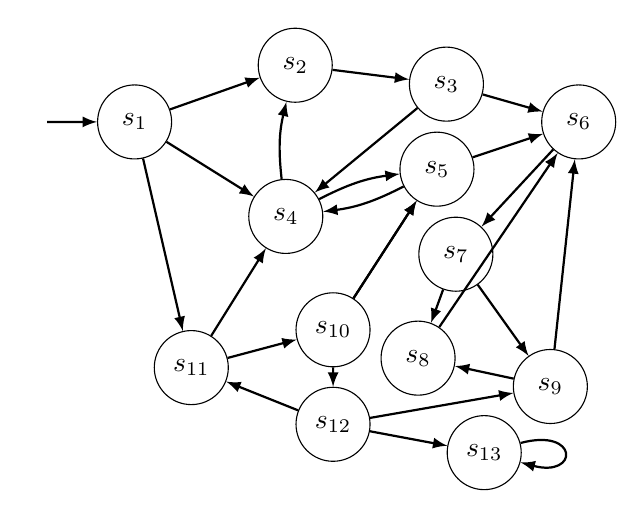
\begin{tikzpicture} [scale=1.2, every initial by arrow/.style={thick}]
		
		style/.mstate={minimum size=2}
			
%		\path
%		(\basex+.3,		\basey) 		node[mstate,initial,initial text=,initial distance=15pt] (s1) 	{$\state_1$} 
%		(\basex+2,		\basey+1.6) 		node[mstate] (s2) 	{$\state_2$} 
%		(\basex+3.6,	\basey+1.4) 	node[mstate] (s3) 	{$\state_3$} 
%		(\basex+1.9,		\basey+0) 		node[mstate] (s4) {$\state_4$} 
%		(\basex+3.5,		\basey+0.5)		node[mstate] (s5) 	{$\state_5$} 
%		(\basex+3.7,		\basey-.4) 		node[mstate] (s6) 	{$\state_6$} 
%		(\basex+5,	\basey) 		node[mstate] (s7) 	{$\state_7$} 
%		(\basex+2.4,	\basey-1.2) 	node[mstate] (s8) 	{$\state_8$} 
%		(\basex+3.3,		\basey-1.5) 	node[mstate] (s9) 	{$\state_9$} 
%		(\basex+.9,		\basey-1.6) 	node[mstate] (s10) 	{$\state_{10}$} 
%		(\basex+4.7,		\basey-1.8) 		node[mstate] (s11) 	{$\state_{11}$} 
%		(\basex+2.4,	\basey-2.2)		node[mstate] (s12) 	{$\state_{12}$} 
%		(\basex+4,		\basey-2.5) 		node[mstate] (s13) 	{$\state_{13}$} 
%		
%		;
		\path
		(\basex+.3,		\basey) 		node[mstate,initial,initial text=,initial distance=15pt] (s1) 	{$\state_1$} 
		(\basex+2,		\basey+1.6) 		node[mstate] (s2) 	{$\state_2$} 
		(\basex+3.6,	\basey+1.4) 	node[mstate] (s3) 	{$\state_3$} 
		(\basex+1.9,		\basey+0) 		node[mstate] (s4) {$\state_4$} 
		(\basex+3.5,		\basey+0.5)		node[mstate] (s5) 	{$\state_5$} 
		(\basex+3.7,		\basey-.4) 		node[mstate] (s6) 	{$\state_7$} 
		(\basex+5,	\basey) 		node[mstate] (s7) 	{$\state_6$} 
		(\basex+2.4,	\basey-1.2) 	node[mstate] (s8) 	{$\state_{10}$} 
		(\basex+3.3,		\basey-1.5) 	node[mstate] (s9) 	{$\state_8$} 
		(\basex+.9,		\basey-1.6) 	node[mstate] (s10) 	{$\state_{11}$} 
		(\basex+4.7,		\basey-1.8) 		node[mstate] (s11) 	{$\state_{9}$} 
		(\basex+2.4,	\basey-2.2)		node[mstate] (s12) 	{$\state_{12}$} 
		(\basex+4,		\basey-2.5) 		node[mstate] (s13) 	{$\state_{13}$} 
		
		;
		
		\path [trans] (s1) edge (s2);
		\path [trans] (s1) edge (s4);
		\path [trans] (s1) edge (s10);
		\path [trans] (s2) edge (s3);
		\path [trans] (s3) edge (s4);
		\path [trans] (s3) edge (s7);
		\path [bendtrans] (s4) edge (s2);
		\path [bendtrans] (s4) edge (s5);
		\path [bendtrans] (s5) edge (s4);
		\path [trans] (s5) edge (s7);
		\path [trans] (s6) edge (s9);
		\path [trans] (s6) edge (s11);
		\path [trans] (s7) edge (s6);
		\path [trans] (s8) edge (s5);
		\path [trans] (s8) edge (s12);
		\path [trans] (s8) edge (s5);
		\path [trans] (s9) edge (s7);
		\path [trans] (s10) edge (s4);
		\path [trans] (s10) edge (s8);
		\path [trans] (s11) edge (s7);
		\path [trans] (s11) edge (s9);
		\path [trans] (s12) edge (s10);
		\path [trans] (s12) edge (s11);
		\path [trans] (s12) edge (s13);

		\path [trans] (s13) edge [loop right] (s13);
 		
%		\path [trans, bend right=25] 		(sbot) 	edge node [midway,above left]		{\actionc} 		(s4);
%		\path [trans] 		(sbot) 	edge node [midway,right]			{\actionb} 		(s3);
%		\path [trans, bend right=25] 		(sbot) 	edge node [midway,left]				{\action} 		(s3);
%		\path [trans, bend left=25](sbot) 	edge node [midway,left]			{\actionb} 		(s5);
%		\path [trans, bend left=45] (sbot) 	edge node [midway,right]		{\actionc} 		(s5);
%		\path [trans,bend right=35] 	(s3) 	edge node [midway,right]	{\actionc} 		(sbot);
%		\path [trans] 	(s3) 	edge node [midway,above left]	{\action} 		(s4);
%		\path [trans] 	(s5) 	edge node [midway,above]	{\actionc} 		(s4);
%		
%		\path [trans] 		(sbot) 	edge [loop, in=15, out=50, looseness=6] node [midway,right] {\action,\actionb} 	(sbot);
%		\path [trans] 		(s3) 	edge [loop right] node [midway,below=4pt] {\actionb} 	(s3);
%		\path [trans] 		(s4) 	edge [loop below] node [midway,below] {\action} 	(s4);
%		\path [trans] 		(s6) 	edge [loop above] node [midway,above] {\actionc} 	(s6);
		
		
		%		midway, at start, near start, very near start, at end, near end, very near end
		
		
	\end{tikzpicture}
\end{document}
	\end{minipage}
	\begin{minipage}{.5\textwidth}		
		\documentclass[tikz,preview]{standalone}
%\usepackage{prelude}

%%%%%%%%%%%%%%%%%%%%%%%%%%%%%%%%%%%% PACKAGES %%%%%%%%%%%%%%%%%%%%%%%%%%%%%%%%%%%%%%%%%%

\usepackage{inputenc,fontenc}
\usepackage[a4paper,margin=3cm]{geometry}
\usepackage[english]{babel}
%\usepackage[german]{babel}
%\usepackage[fixlanguage]{babelbib}


\usepackage{bbold}
\usepackage{amsthm}
\usepackage{amsmath}
\usepackage{amssymb} % doteqdot
\usepackage[dvipsnames]{xcolor}
\usepackage{standalone}
\usepackage{tikz}[mode=buildnew]
\usepackage{cite}
\usepackage{xspace}
\usepackage{relsize}
\usepackage{mathtools} % mathclap
%\usepackage{MnSymbol}
\usepackage{hyperref}
\usepackage{url}
\usepackage{listings} % for code
\usepackage[T1]{fontenc} %<
\hypersetup{
	colorlinks,
	citecolor=black,
	filecolor=black,
	linkcolor=black,
	urlcolor=black
}
\usepackage{pgfplots}
\pgfplotsset{compat=1.18}
%\usepackage{courier} %% Sets font for listing as Courier. But also for url and texttt!
\usepackage{listings, xcolor}
\usepackage{graphicx}
\usepackage{subcaption}

\usetikzlibrary{calc}
%\usepackage{xparse} % \newDocumentCommand for multiple optional arguments
%\usepackage{titlecaps}



%%%%%%%%%%%%%%%%%%%%%%%%%%%%%%%%%%%% THEOREMSTYLES %%%%%%%%%%%%%%%%%%%%%%%%%%%%%%%%%%

\theoremstyle{definition}
\newtheorem{definition}{Definition}[section]
\newtheorem{exmp}{Beispiel}[section]
%\AfterEndEnvironment{definition}{\noindent\ignorespaces}

\theoremstyle{theorem}
\newtheorem{theorem}{Satz}[section]
\newtheorem{proposition}{Proposition}[section]
%\AfterEndEnvironment{theorem}{\noindent\ignorespaces}

\theoremstyle{korollary}
\newtheorem{korollary}{Korollar}[section]
%\AfterEndEnvironment{korollary}{\noindent\ignorespaces}


\tikzset{
	mstate/.style={draw, circle, minimum size=.94cm}, 
	gstate/.style={draw, rectangle, minimum size=.8cm},
	varstate/.style={draw,rectangle, rounded corners, minimum size=1}, 
	trans/.style={draw, ->, thick},
	bendtrans/.style={draw, ->, thick, bend left=10},
	bendtransr/.style={draw, ->, thick, bend right=10},
	init/.style={initial, initial distance=6pt, initial text=},
	every loop/.style={min distance=5pt, looseness=8},
	>=latex
}
\usetikzlibrary{automata,positioning}

%auto shift/.style={auto=right,->,
%	to path={ let \p1=(\tikztostart),\p2=(\tikztotarget),
%		\n1={atan2(\y2-\y1,\x2-\x1)},\n2={\n1+180}
%		in ($(\tikztostart.{\n1})!1mm!270:(\tikztotarget.{\n2})$) -- 
%		($(\tikztotarget.{\n2})!1mm!90:(\tikztostart.{\n1})$) \tikztonodes}},

%%%%%%%%%%%%%%%%%%%%%%%%%%%%%%%%%%% MY MACROS %%%%%%%%%%%%%%%%%%%%%%%%%%%%%%%%%%%%%%%%%
%formatting
\newcommand{\comment}[2]{{\color{#1}#2}}
\newcommand{\redcomment}[1]{{\color{red}#1}}
\newcommand{\purpcomment}[1]{{\color{pink}#1}}
\newcommand{\bluecomment}[1]{{\color{blue}#1}}
\newcommand{\mt}[1]{\ensuremath{{#1}}\xspace}
\newcommand{\mynewcommand}[2]{\newcommand{#1}{\mt{#2}}} %% currently not used becaue of ide highlighting
\newcommand{\arr}{\mt{\to}}

%model checking terms
\newcommand{\mimicrel}{\mt{\mathcal{R}}}
\newcommand{\bisimeq}{\mt{\;\!\sim\;\!}}
\newcommand{\simorder}{\mt{\;\!\preceq\;\!}}
\newcommand{\simequiv}{\mt{\;\!\simeq\;\!}} %command already defined
\newcommand{\relts}{\mt{\;\!\bullet_{_{\tiny{TS}}}\;\!}}
\newcommand{\rel}{\mt{\;\!\bullet\;\!}}

%own names
\newcommand{\nm}[1]{#1\xspace}
\newcommand{\mdpN}{\nm{MDP}}
\newcommand{\mdpsN}{\nm{MDPs}}
\newcommand{\viewN}{\nm{view}}
\newcommand{\viewNC}{\nm{View}}
\newcommand{\viewsN}{\nm{views}}
\newcommand{\viewsNC}{\nm{Views}}
\newcommand{\grpfctsubN}{\nm{detached grouping function}}
\newcommand{\grpfctsubNC}{\nm{detached grouping function}}
\newcommand{\grpfctsubNCC}{\nm{Detached Grouping Function}}
\newcommand{\grpfctN}{\nm{grouping function}}
\newcommand{\grpfctNC}{\nm{Grouping function}}
\newcommand{\grpfctNCC}{\nm{Grouping Function}}
\newcommand{\grpfctsN}{\nm{grouping functions}}
\newcommand{\grpfctsNC}{\nm{Grouping functions}}
\newcommand{\grpfctsNCC}{\nm{Grouping Functions}}
\newcommand{\stmimicN}{\nm{state-mimic}}
\newcommand{\stmimicsN}{\nm{state-mimics}}
\newcommand{\stmimickingN}{\nm{state-mimicking}}
\newcommand{\stmimickedN}{\nm{state-mimicked}}
%\newcommand{\chosenphtypeNCC}{\nm{Transition System}}
%\newcommand{\chgphNC}{\nm{Transition system}}
%\newcommand{\chgphN}{\nm{transition system}}
%\newcommand{\chgphsNCC}{\nm{Transition Systems}}
%\newcommand{\chgphsNC}{\nm{Transition systems}}
%\newcommand{\chgphsN}{\nm{transition systems}}
\newcommand{\chgphNCC}{\nm{MDP}}
\newcommand{\chgphNC}{\nm{MDP}}
\newcommand{\chgphN}{\nm{MDP}}
\newcommand{\achgphN}{\nm{an MDP}}
\newcommand{\chgphsNCC}{\nm{MDPs}}
\newcommand{\chgphsNC}{\nm{MDPs}}
\newcommand{\chgphsN}{\nm{MDPs}}
\newcommand{\parllcompN}{\nm{parallel composition}}
\newcommand{\parllcompNC}{\nm{Parallel composition}}
\newcommand{\parllcompNCC}{\nm{Parallel Composition}}
\newcommand{\parllcompsN}{\nm{parallel compositions}}
\newcommand{\parllcompsNC}{\nm{Parallel compositions}}
\newcommand{\parllcompsNCC}{\nm{Parallel Compositions}}
\newcommand{\sccN}{\nm{SCC}}
\newcommand{\sccsN}{\nm{SCCs}}
\newcommand{\bsccN}{\nm{BSCC}}
\newcommand{\bsccsN}{\nm{BSCCs}}
\newcommand{\jgrapht}{\nm{jGraphtT}}

\newcommand{\outactident}{\nm{OutActionsIdent}}

%names
\newcommand{\iffN}{\nm{if and only if}}
\newcommand{\tsN}{\nm{TS}}

%% outactions identical
\newcommand{\outactidentstrong}{\nm{strong}}
\newcommand{\outactidentweak}{\nm{weak}}

% CORE DEFINITIONS
\newcommand{\grpfct}[1][\viewppty]{\mt{F_{#1}}}
\newcommand{\grpfctsub}[1][\viewppty]{\mt{\tilde{F}_{#1}}}
%\newcommand{\grpfctimg}[1]{\mt{{\grpfct}[{#1}]}}
%\newcommand{\fctimg}[2]{\mt{{#1}[{#2}]}}
\newcommand{\eqrelview}{\mt{R}}
\newcommand{\eqclassv}[1][\state]{\mt{\eqclass{#1}{\eqrelview}}}
\newcommand{\eqclasssetv}[1][\states]{\mt{{#1}/\eqrelview}} %OLD: \bigcup_{\state \in \states} \eqclassv
\newcommand{\viewid}{\mt{\mdp}}
\newcommand{\view}[1][\viewppty]{\mt{\viewid_{#1}}}
\newcommand{\imggrp}{\mt{\arbset}}
\newcommand{\imggrpsub}{\mt{X}}
\newcommand{\viewppty}{\mt{\theta}}
\newcommand{\pll}{\mt{\;\!\pllpure\;\!}}
\newcommand{\pllrev}{\mt{\pllpure^{-1}}}
\newcommand{\pllpure}{\mt{||}}
\newcommand{\compselectset}{\mt{Z}}
\newcommand{\compselectpure}{\mt{\pllpure_\compselectset}}
\newcommand{\compselect}{\mt{\;\pllpure_\compselectset\;}}
\newcommand{\remstates}{\mt{\bigcup_{\state \in \states \setminus \states_1}\{\{\state\}\}}}
\newcommand{\nogroupstates}[1][\states_2]{\mt{\bigcup_{\state \in \states \setminus {#1}}\{\{\state\}\}}}
\newcommand{\remelem}{\mt{\bullet}}
\newcommand{\nogroupset}{\mt{\xi}}
\newcommand{\remset}{\mt{\{\remelem\}}}
\newcommand{\gfctpll}{\mt{\grpfct[\pll]}}
\newcommand{\group}{\mt{\top}}
\newcommand{\imggrpbinview}{\mt{\{\remelem, \notppty\}}}
\newcommand{\viewappset}{\mt{\tilde{\states}}}
\newcommand{\hasppty}{\mt{\top}}
\newcommand{\notppty}{\mt{\bot}}
\newcommand{\disregardelem}{\mt{\Delta}}
\newcommand{\disregardelements}{\mt{{\disregardelem_1, \dots, \disregardelem_n}}}



%\newcommand{\mdp}{def}\mdp
%\newcommand{\mdpdef}



% EXAMPLE VIEWS
\newcommand{\pptyatomicprops}{\mt{\atomicprops}}
\newcommand{\pptyinitstates}{\mt{\initstates}}
\newcommand{\pptyinactsetsize}{\mt{|\inacts(\state)|}}
\newcommand{\pptyhasoutact}{\mt{\exists\outact}}
\newcommand{\pptyminoutact}[2]{\mt{#1\leq#2}}
\newcommand{\pptymaxoutact}[2]{\mt{#2\leq#1}}
\newcommand{\pptyspanoutact}[3]{\mt{#1\leq#2\leq#3}}
\newcommand{\pptyoutactsetsize}{\mt{|\outacts(\state)|}}
\newcommand{\pptyoutactsingle}{\mt{|\outacts(\state)|_1}}
\newcommand{\pptystrongoutactident}{\mt{\outacts(\state)_=}}
\newcommand{\pptyweakoutactident}{\mt{\outacts(\state)_\approx}}
\newcommand{\pptyhasinact}{\mt{\exists\inact}}
\newcommand{\pptymininact}[2]{\mt{#1\leq#2}}
\newcommand{\pptymaxinact}[2]{\mt{#2\leq#1}}
\newcommand{\pptyspaninact}[3]{\mt{#1\leq#2\leq#3}}
\newcommand{\pptyinactsingle}{\mt{|\inacts(\state)|_1}}
\newcommand{\pptystronginactident}{\mt{\inacts(\state)_=}}
\newcommand{\pptyweakinactident}{\mt{\inacts(\state)_\approx}}
\newcommand{\pptyparamvalueseq}{\mt{\var = \varval}}
\newcommand{\pptyparamvaluesneq}{\mt{\var \neq \varval}}
\newcommand{\pptyparamdnf}{\mt{VarDNF}}
\newcommand{\pptyparamcnf}{\mt{VarCNF}}
\newcommand{\pptyparamvalueseqopt}{\mt{\var = \varval}}
\newcommand{\pptyparamvalident}{\mt{Var:\varval}}
\newcommand{\pptydistance}{\mt{\distpath}}
\newcommand{\pptydistancerev}{\mt{\distpathrev}}
\newcommand{\pptydistancebi}{\mt{\distpathbi}}
\newcommand{\pptyhascycle}{\mt{\exists\cycle}}
\newcommand{\pptyexactactcycle}{\mt{\{\cycle_{\action,n}\}}}
\newcommand{\pptycycleset}{\mt{\cup{\{\state\}_\cycle}}}
\newcommand{\pptyexactcycle}{\mt{\{\cycle_n\}}}
\newcommand{\pptyscc}{\mt{scc}}
\newcommand{\pptybscc}{\mt{bscc}}
\newcommand{\pptyprop}{\mt{\redcomment{?}}}
\newcommand{\pptyident}{id}


\newcommand{\gfctatomicprops}{\mt{\grpfct[\pptyatomicprops]}}
\newcommand{\gfctinitstates}{\mt{\grpfct[\pptyinitstates]^\hasppty}}
\newcommand{\gfcthasoutaction}{\mt{\grpfct[\pptyhasoutact]^\hasppty}}
\newcommand{\gfctminoutaction}{\mt{\grpfct[\pptyminoutact{\numoutact}{\outact}]^\hasppty}}
\newcommand{\gfctmaxoutaction}{\mt{\grpfct[\pptymaxoutact{\numoutact}{\outact}]^\hasppty}}
\newcommand{\gfctspanoutaction}{\mt{\grpfct[\pptyspanoutact{\numoutactb}{\outact}{\numoutact}]^\hasppty}}
\newcommand{\gfctoutactsetsize}{\mt{\grpfct[\pptyoutactsetsize]}}
\newcommand{\gfctoutactsingle}{\mt{\grpfct[\pptyoutactsingle]^\notppty}}
\newcommand{\gfctstrongoutactident}{\mt{\grpfct[\pptystrongoutactident]}}
\newcommand{\gfctweakoutactident}{\mt{\grpfct[\pptyweakoutactident]}}
\newcommand{\gfcthasinaction}{\mt{\grpfct[\pptyhasinact]^\hasppty}}
\newcommand{\gfctmininaction}{\mt{\grpfct[\pptymininact{\numinact}{\inact}]^\hasppty}}
\newcommand{\gfctmaxinaction}{\mt{\grpfct[\pptymaxinact{\numinact}{\inact}]^\hasppty}}
\newcommand{\gfctspaninaction}{\mt{\grpfct[\pptyspaninact{\numinactb}{\inact}{\numinact}]^\hasppty}}
\newcommand{\gfctinactsetsize}{\mt{\grpfct[\pptyinactsetsize]}}
\newcommand{\gfctinactsingle}{\mt{\grpfct[\pptyinactsingle]^\notppty}}
\newcommand{\gfctstronginactident}{\mt{\grpfct[\pptystronginactident]}}
\newcommand{\gfctweakinactident}{\mt{\grpfct[\pptyweakinactident]}}
\newcommand{\gfctparamvalueseq}{\mt{\grpfct[\pptyparamvalueseq]^\hasppty}}
\newcommand{\gfctparamvaluesneq}{\mt{\grpfct[\pptyparamvaluesneq]^\hasppty}}
\newcommand{\gfctparamdnf}{\mt{\grpfct[\pptyparamdnf]^\hasppty}}
\newcommand{\gfctparamcnf}{\mt{\grpfct[\pptyparamcnf]^\hasppty}}
\newcommand{\gfctparamvalueseqopt}{\mt{\pptyparamvalueseqopt}}
\newcommand{\gfctparamvalident}{\mt{\grpfct[\pptyparamvalident]}}
\newcommand{\gfctdistance}{\mt{\grpfct[\pptydistance]}}
\newcommand{\gfctdistancerev}{\mt{\grpfct[\pptydistancerev]}}
\newcommand{\gfctdistancebi}{\mt{\grpfct[\pptydistancebi]}}
\newcommand{\gfcthascycle}{\mt{\grpfct[\pptyhascycle]}}
\newcommand{\gfctexactcycle}{\mt{\grpfct[\pptyexactcycle]}}
\newcommand{\gfctcycleset}{\mt{\grpfct[\pptycycleset]}}
\newcommand{\gfctexactactcycle}{\mt{\grpfct[\pptyexactactcycle]}}
\newcommand{\gfctscc}{\mt{\grpfct[\pptyscc]}}
\newcommand{\gfctbscc}{\mt{\grpfct[\pptybscc]}}
\newcommand{\gfctprop}{\mt{\grpfct[\pptyprop]}}
\newcommand{\gfctident}{\mt{\grpfct[\pptyident]}}

\newcommand{\gfctsubatomicprops}{\mt{\grpfctsub[\pptyatomicprops]}}
\newcommand{\gfctsubinitstates}{\mt{\grpfctsub[\pptyinitstates]^\hasppty}}
\newcommand{\gfctsubhasoutaction}{\mt{\grpfctsub[\pptyhasoutact]^\hasppty}}
\newcommand{\gfctsubminoutaction}{\mt{\grpfctsub[\pptyminoutact{\numoutact}{\outact}]^\hasppty}}
\newcommand{\gfctsubmaxoutaction}{\mt{\grpfctsub[\pptymaxoutact{\numoutact}{\outact}]^\hasppty}}
\newcommand{\gfctsubspanoutaction}{\mt{\grpfctsub[\pptyspanoutact{\numoutactb}{\outact}{\numoutact}]^\hasppty}}
\newcommand{\gfctsuboutactsetsize}{\mt{\grpfctsub[\pptyoutactsetsize]}}
\newcommand{\gfctsuboutactsingle}{\mt{\grpfctsub[\pptyoutactsingle]^\notppty}}
\newcommand{\gfctsubstrongoutactident}{\mt{\grpfctsub[\pptystrongoutactident]^\hasppty}}
\newcommand{\gfctsubweakoutactident}{\mt{\grpfctsub[\pptyweakoutactident]^\hasppty}}
\newcommand{\gfctsubhasinaction}{\mt{\grpfctsub[\pptyhasinact]}}
\newcommand{\gfctsubmininaction}{\mt{\grpfctsub[\pptymininact{\numinact}{\inact}]}}
\newcommand{\gfctsubmaxinaction}{\mt{\grpfctsub[\pptymaxinact{\numinact}{\inact}]}}
\newcommand{\gfctsubspaninaction}{\mt{\grpfctsub[\pptyspaninact{\numinactb}{\inact}{\numinact}]}}
\newcommand{\gfctsubinactsetsize}{\mt{\grpfctsub[\pptyinactsetsize]^\hasppty}}
\newcommand{\gfctsubinactsingle}{\mt{\grpfctsub[\pptyinactsingle]^\notppty}}
\newcommand{\gfctsubstronginactident}{\mt{\grpfctsub[\pptystronginactident]}}
\newcommand{\gfctsubweakinactident}{\mt{\grpfctsub[\pptyweakinactident]}}
\newcommand{\gfctsubparamvalueseq}{\mt{\grpfctsub[\pptyparamvalueseq]^\hasppty}}
\newcommand{\gfctsubparamvaluesneq}{\mt{\grpfctsub[\pptyparamvaluesneq]^\hasppty}}
\newcommand{\gfctsubparamdnf}{\mt{\grpfctsub[\pptyparamdnf]^\hasppty}}
\newcommand{\gfctsubparamcnf}{\mt{\grpfctsub[\pptyparamcnf]^\hasppty}}
\newcommand{\gfctsubparamvalueseqopt}{\mt{\pptyparamvalueseqopt}}
\newcommand{\gfctsubparamvalident}{\mt{\grpfctsub[\pptyparamvalident]}}
\newcommand{\gfctsubdistance}{\mt{\grpfctsub[\pptydistance]}}
\newcommand{\gfctsubdistancerev}{\mt{\grpfctsub[\pptydistancerev]}}
\newcommand{\gfctsubdistancebi}{\mt{\grpfctsub[\pptydistancebi]}}
\newcommand{\gfctsubhascycle}{\mt{\grpfctsub[\pptyhascycle]^\hasppty}}
\newcommand{\gfctsubexactcycle}{\mt{\grpfctsub[\pptyexactcycle]}}
\newcommand{\gfctsubcycleset}{\mt{\grpfctsub[\pptycycleset]}}
\newcommand{\gfctsubexactactcycle}{\mt{\grpfctsub[\pptyexactactcycle]}}
\newcommand{\gfctsubscc}{\mt{\grpfctsub[\pptyscc]}}
\newcommand{\gfctsubbscc}{\mt{\grpfctsub[\pptybscc]}}
\newcommand{\gfctsubprop}{\mt{\grpfctsub[\pptyprop]}}
\newcommand{\gfctsubident}{\mt{\grpfctsub[\pptyident]}}


\newcommand{\viewatomicprops}{\mt{\view[\pptyatomicprops]}}
\newcommand{\viewinitstates}{\mt{\view[\pptyinitstates]^\hasppty}}
\newcommand{\viewhasoutaction}{\mt{\view[\pptyhasoutact]^\hasppty}}
\newcommand{\viewminoutaction}{\mt{\view[\pptyminoutact{\numoutact}{\outact}]^\hasppty}}
\newcommand{\viewmaxoutaction}{\mt{\view[\pptymaxoutact{\numoutact}{\outact}]^\hasppty}}
\newcommand{\viewspanoutaction}{\mt{\view[\pptyspanoutact{\numoutactb}{\outact}{\numoutact}]^\hasppty}}
\newcommand{\viewoutactsetsize}{\mt{\view[\pptyoutactsetsize]}}
\newcommand{\viewoutactsingle}{\mt{\view[\pptyoutactsingle]^\notppty}}
\newcommand{\viewstrongoutactident}{\mt{\view[\pptystrongoutactident]}}
\newcommand{\viewweakoutactident}{\mt{\view[\pptyweakoutactident]}}
\newcommand{\viewhasinaction}{\mt{\view[\pptyhasinact]^\hasppty}}
\newcommand{\viewmininaction}{\mt{\view[\pptymininact{\numinact}{\inact}]^\hasppty}}
\newcommand{\viewmaxinaction}{\mt{\view[\pptymaxinact{\numinact}{\inact}]^\hasppty}}
\newcommand{\viewspaninaction}{\mt{\view[\pptyspaninact{\numinactb}{\inact}{\numinact}]^\hasppty}}
\newcommand{\viewinactsetsize}{\mt{\view[\pptyinactsetsize]}}
\newcommand{\viewinactsingle}{\mt{\view[\pptyinactsingle]^\notppty}}
\newcommand{\viewstronginactident}{\mt{\view[\pptystronginactident]}}
\newcommand{\viewweakinactident}{\mt{\view[\pptyweakinactident]}}
\newcommand{\viewparamvalueseq}{\mt{\view[\pptyparamvalueseq]}}
\newcommand{\viewparamvaluesneq}{\mt{\view[\pptyparamvaluesneq]}}
\newcommand{\viewparamdnf}{\mt{\view[\pptyparamdnf]^\hasppty}}
\newcommand{\viewparamcnf}{\mt{\view[\pptyparamcnf]^\hasppty}}
\newcommand{\viewparamvalueseqopt}{\mt{\pptyparamvalueseqopt}}
\newcommand{\viewparamvalident}{\mt{\view[\pptyparamvalident]}}
\newcommand{\viewdistance}{\mt{\view[\pptydistance]}}
\newcommand{\viewdistancerev}{\mt{\view[\pptydistancerev]}}
\newcommand{\viewdistancebi}{\mt{\view[\pptydistancebi]}}
\newcommand{\viewhascycle}{\mt{\view[\pptyhascycle]}}
\newcommand{\viewexactcycle}{\mt{\view[\pptyexactcycle]}}
\newcommand{\viewcycleset}{\mt{\view[\pptycycleset]}}
\newcommand{\viewexactactcycle}{\mt{\view[\pptyexactactcycle]}}
\newcommand{\viewscc}{\mt{\view[\pptyscc]}}
\newcommand{\viewbscc}{\mt{\view[\pptybscc]}}
\newcommand{\viewprop}{\mt{\view[\pptyprop]}}
\newcommand{\viewident}{\mt{\view[\pptyident]}}

%\newcommand{\viewatomicprops}{\mt{\view[\atomicprops]}}
%\newcommand{\viewinitstates}{\mt{\view[\initstates]}}
%\newcommand{\viewhasoutaction}{\mt{\view[\pptyhasoutact]}}
%\newcommand{\viewminoutaction}{\mt{\view[\pptyminoutact{\numoutact}{\outact}]}}
%\newcommand{\viewmaxoutaction}{\mt{\view[\pptymaxoutact{\numoutact}{\outact}]}}
%\newcommand{\viewspanoutaction}{\mt{\view[\pptyspanoutact{\numoutactb}{\outact}{\numoutact}]}}
%\newcommand{\viewoutactsetsize}{\mt{\view[\pptyoutactsetsize]}}
%\newcommand{\viewoutactsingle}{\mt{\view[\pptyoutactsingle]}}
%\newcommand{\viewstrongoutactident}{\mt{\view[\outacts(\state)_=]}}
%\newcommand{\viewweakoutactident}{\mt{\view[\outacts(\state)_\approx]}}
%\newcommand{\viewhasinaction}{\mt{\view[\pptyhasinact]}}
%\newcommand{\viewmininaction}{\mt{\view[\pptymininact{\numinact}{\inact}]}}
%\newcommand{\viewmaxinaction}{\mt{\view[\pptymaxinact{\numinact}{\inact}]}}
%\newcommand{\viewspaninaction}{\mt{\view[\pptyspaninact{\numinactb}{\inact}{\numinact}]}}
%\newcommand{\viewinactsetsize}{\mt{\view[\pptyinactsetsize]}}
%\newcommand{\viewinactsingle}{\mt{\view[\pptyinactsingle]}}
%\newcommand{\viewstronginactident}{\mt{\view[\inacts(\state)_=]}}
%\newcommand{\viewweakinactident}{\mt{\view[\inacts(\state)_\approx]}}
%\newcommand{\viewparamvalueseq}{\mt{\view[\var = \varval]}}
%\newcommand{\viewparamvaluesneq}{\mt{\view[\var \neq \varval]}}
%\newcommand{\viewparamdnf}{\mt{\view[VarDNF]}}
%\newcommand{\viewparamcnf}{\mt{\view[VarCNF]}}
%\newcommand{\viewparamvalident}{\mt{\view[\pptyparamvalident]}}
%\newcommand{\viewdistance}{\mt{\view[\pptydistance]}}
%\newcommand{\viewhascycle}{\mt{\view[\exists\cycle]}}
%\newcommand{\viewexactcycle}{\mt{\view[\pptyexactcycle]}}
%\newcommand{\viewcycleset}{\mt{\view[\pptycycleset]}}
%\newcommand{\viewexactactcycle}{\mt{\view[\pptyexactactcycle]}}
%\newcommand{\viewscc}{\mt{\view[scc]}}
%\newcommand{\viewbscc}{\mt{\view[bscc]}}

%actions
\newcommand{\numoutact}{\mt{n}}
\newcommand{\numoutactb}{\mt{m}}
\newcommand{\numinact}{\mt{n}}
\newcommand{\numinactb}{\mt{m}}

\newcommand{\predmaxoutact}[1][\numoutact]{\mt{Q_{\outact\leq#1}(\state,\state_1, \dots, \state_{#1+1})}}
\newcommand{\predminoutact}[1][\numoutact]{\mt{Q_{#1\leq\outact}(\state,\state_1, \dots, \state_{#1})}}
\newcommand{\formoutact}[1][\state]{\mt{C_{#1,\outact}}}
\newcommand{\predmaxinact}[1][\numinact]{\mt{Q_{\inact\leq#1}(\state,\state_1, \dots, \state_{#1+1})}}
\newcommand{\predmininact}[1][\numinact]{\mt{Q_{#1\leq\inact}(\state,\state_1, \dots, \state_{#1})}}

\newcommand{\outact}[1][\action]{\mt{\overrightarrow{#1}}}
\newcommand{\outacts}{\mt{\overrightarrow{\actions}}}
\newcommand{\inact}{\mt{\overleftarrow{\action}}}
\newcommand{\inacts}[1][\action]{\mt{\overleftarrow{#1}}}

%%Parameters
\newcommand{\vars}[1][\mdp]{\mt{V\!ar_{#1}}}
\newcommand{\var}{\mt{x}}
\newcommand{\varstate}[1][]{\mt{\var_{\state#1}}}
\newcommand{\varval}{\mt{a}}
\newcommand{\vareval}[1][\mdp]{\mt{V\!arEval_{#1}}}
\newcommand{\varevalimg}[1][\mdp]{\mt{\vareval[#1][\states,\vars]}}
\newcommand{\varevalimgset}{\mt{\arbset}}
\newcommand{\someparam}{\mt{\tilde{x}}}
\newcommand{\eqorneq}{\mt{\;\doteqdot\;}}
\newcommand{\varstyle}[2]{\mt{\langle#1,#2\rangle}}




%\makeatletter
%\newcommand{\overleftrightsmallarrow}{\mathpalette{\overarrowsmall@\leftrightarrowfill@}}
%\newcommand{\overrightsmallarrow}{\mathpalette{\overarrowsmall@\rightarrowfill@}}
%\newcommand{\overleftsmallarrow}{\mathpalette{\overarrowsmall@\leftarrowfill@}}
%\newcommand{\overarrowsmall@}[3]{%
%	\vbox{%
%		\ialign{%
%			##\crcr
%			#1{\smaller@style{#2}}\crcr
%			\noalign{\nointerlineskip}%
%			$\m@th\hfil#2#3\hfil$\crcr
%		}%
%	}%
%}
%\def\smaller@style#1{%
%	\ifx#1\displaystyle\scriptstyle\else
%	\ifx#1\textstyle\scriptstyle\else
%	\scriptscriptstyle
%	\fi
%	\fi
%}
%\makeatother
%\newcommand{\te}[1]{\overleftrightsmallarrow{#1}}

% Distance
\newcommand{\fctdist}{\mt{distance}}
\newcommand{\fctdistdefault}{\mt{\fctdist(\chgph, \smstates, \grandist)}}
\newcommand{\distval}{\mt{d}}
\newcommand{\grandist}{\mt{n}}
\let\path\oldpath
\newcommand{\path}{\mt{P}}
\newcommand{\pathbi}{\mt{\bar{\path}}}
\newcommand{\pathsecfull}{\mt{(\state_0, \action_0, \state_1, \action_1, \dots, \action_{n}, \state_{n+1})}}
\newcommand{\lenpath}{\mt{len}}
\newcommand{\pfirst}{\mt{first}}
\newcommand{\plast}{\mt{last}}
\newcommand{\pathset}{\mt{\path_\chgph}}
\newcommand{\pathbiset}{\mt{\pathbi_\chgph}}
\newcommand{\distpath}{\mt{\overrightarrow{dist}}}
\newcommand{\distpathrev}{\mt{\overleftarrow{dist}}}
\newcommand{\distpathbi}{\mt{\overline{dist}}}
%Cycles
\newcommand{\cyclesecfull}{\mt{(\state_0, \action_0, \state_1, \action_1, \dots, \action_{n-1}, \state_0)}}
\newcommand{\fctfindcycles}{\mt{findCycles}}
\newcommand{\cycle}{\mt{C}}
\newcommand{\cycleset}{\mt{\cycle_{\mdp, n}}}
\newcommand{\lencycle}{\mt{len}}
% strongly connected components
\newcommand{\scc}{\mt{T}}
\newcommand{\setscc}{\mt{SCC_{\chgph,n}}}
\newcommand{\setbscc}{\mt{BSCC_{\chgph,n}}}

% properties
\newcommand{\propfct}{\mt{f}}

% all Systems
\newcommand{\chgph}{\mt{\mdp}}
\newcommand{\chgphtuple}{\mt{\mdptuple}}
\newcommand{\chgphtupledist}{\mt{\mdptupledist}}

\newcommand{\states}{\mt{S}}
\newcommand{\actions}{\mt{Act}}
\newcommand{\atomicprops}{\mt{AP}}
\newcommand{\labelingfct}{\mt{L}}
\newcommand{\init}{\mt{\initdistrib}} % use MDP % refers to the underlying set
\newcommand{\trans}{\mt{\probtfunc}} % use MDP % refers to the underlying set
\newcommand{\smstates}{\mt{\tilde{\states}}}


\newcommand{\state}{\mt{s}}
\newcommand{\action}{\mt{\alpha}}
\newcommand{\actionb}{\mt{\beta}}
\newcommand{\actionc}{\mt{\gamma}}
\newcommand{\smstate}{\mt{\tilde{\state}}}



% transition sysstems
\newcommand{\ts}{\mt{TS}}
\newcommand{\transitionrel}{\mt{\longrightarrow}}
\newcommand{\initstates}{\mt{I}}
\newcommand{\transitionsystem}{\mt
	{(\states, \actions, \transitionrel, \initstates, \atomicprops, \labelingfct)}
}
\newcommand{\tstupledist}{\mt{(\states', \actions',\transitionrel', \initstates', \labelingfct')}}


%Markov chains and MDP
\newcommand{\mdp}{\mt{\autm}}
\newcommand{\mdptuple}{\mt{(\states, \actions, \probtfunc, \initdistrib, \atomicprops, \labelingfct)}}
\newcommand{\mdptupledist}{\mt{(\states', \actions', \probtfunc', \initdistrib', \atomicprops', \labelingfct')}}
\newcommand{\autm}{\mt{\mathcal{M}}}
\newcommand{\probtfunc}{\mt{\textbf{P}}}
\newcommand{\initdistrib}{\mt{\iota_{init}}}


%maths
\newcommand{\powerset}[1]{\mt{\mathcal{P}(#1)}}
\newcommand{\eqclass}[2]{\mt{[#1]_{#2}}}%{\mt{#1 / #2}}
\newcommand{\impr}{\mt{\hspace{3mm}\Rightarrow\hspace{2mm}}}
\newcommand{\impl}{\mt{\hspace{3mm}\Leftarrow\hspace{2mm}}}
\newcommand{\natnums}{\mt{\mathbb{N}}} 
\newcommand{\realnums}{\mt{\mathbb{R}}}
\newcommand{\intmodn}[1][n]{\mt{\mathbb{Z}_{#1}}}
\newcommand{\arbset}{\mt{M}}
\newcommand{\bigsum}[2][]{\mt{\mathlarger{\sum}_{#2}^{#1}}}
\newcommand{\bbigsum}[2][]{\mt{\mathlarger{\mathlarger{\sum}}_{#2}^{#1}}}
\newcommand{\invimage}[2]{#1^{\mt{-1}(#2)}}
\newcommand{\img}{\mt{Img}}
\newcommand{\cond}{\mt{\,|\,}}

%tickz
%% \definecolor{darkred}{RGB}{196, 42, 42}

%implementation
\newcommand{\pmcvis}{\nm{PMC-Vis}}



\begin{document}
	\newcommand{\basex}{0}
	\newcommand{\basey}{0}
	\newcommand{\createstate}[3]{\node[draw, circle, minimum size=1cm] (#1) at (#2) {#3}}
	
	
	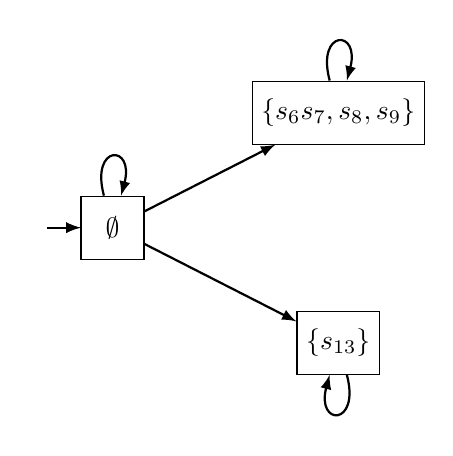
\begin{tikzpicture} [scale=2, every initial by arrow/.style={thick}]
		
		
		\path
		(\basex,		\basey) 		node[gstate,init, initial left] (sbot) 	{$\emptyset$} 
		
		;
		
		\node[gstate, above right = 30pt and 70pt of sbot, anchor=center] (t1) 	{$\{\state_6 \state_7, \state_8, \state_9\}$};
		\node[gstate, below right = 30pt and 70pt of sbot, anchor=center] (t2) 	{$\{\state_{13}\}$};
			
		
		\path [trans] 		(sbot) 	edge node [midway,above]	{} 		(t1);		
		\path [trans] 	(sbot) 	edge node [midway,above]	{} 		(t2);		
%		\path [bendtrans] 	(t2) 	edge node [midway,above]	{} 		(sbot);		
				
		\path [trans] (sbot)	edge [loop above] (bot);
		\path [trans] (t1)	edge [loop above] (t1);
		\path [trans] (t2)	edge [loop below] (t1);
		
		
	\end{tikzpicture}
\end{document}
	\end{minipage}
	\caption{Simplified representations of \mdp (left) and the \viewN \viewbscc on it (right)}
	\label{fig:bsccAfter}  
\end{figure}

In the implementation strongly connected components are determined using the algorithm of Gabow, afterwards filtering those \sccsN that have only transitions to states within the \sccN. Equality, equivalence classes and the new state set are constructed analogously to the view \viewscc.

\subsection{Utilizing the MDP Result Table}
In this section we will discuss \viewsN utilizing the result table. The actual implementation is relies on one powerful \viewN that can set to perform arbitrary actions using model checking results.

\redcomment{needhelp Understanding Cluster}

	
\end{document} 
